\documentclass[10pt,a4paper,twoside]{book}

\input{../../../Libri/template_dispense.tex}



%%%%%%%% ESERCIZI

\usepackage{titlesec}
\usepackage{titletoc}
\usepackage{etoolbox}

%\renewcommand{\thesection}{\arabic{section}}
%\renewcommand{\thesubsection}{\arabic{subsection}}
%\renewcommand{\thechapter}{\arabic{chapter}}

%\titleformat{\section}{\normalfont\LARGE\bfseries}{}{0em}{} % \LARGE anziche' \Large
%\titleformat{\subsection}{\normalfont\large\bfseries}{}{0em}{}

%\newcommand{\Esercizio}[1]{\subsection{Esercizio~\thechapter.\thesubsection~#1}}
%\newcommand{\Soluzione}{\subsection{Soluzione~\thechapter.\thesubsection}}
\newcommand{\Esercizio}[1]{\subsection{Esercizio~#1}}
\newcommand{\Soluzione}{\subsection{Soluzione}}

\newcommand{\ParteEsercizi}{\section{Esercizi}}
\newcommand{\ParteSoluzioni}{\section{Soluzioni}}

% MI ASSICURO QUESTA COSA IMPORTANTE

\setcounter{secnumdepth}{2}
%\setcounter{tocdepth}{1}
\setcounter{tocdepth}{1}


%%%%%%%%%%%%%%%%%%%%

	\usepackage{geometry}
	\geometry{
		nomarginpar, % Toglie doppi margini
		margin=1in, % Imposta i margini a 1 inch
	}

\usepackage{chngcntr}
\counterwithout{figure}{chapter}
\counterwithout{equation}{chapter}

\allowdisplaybreaks[4] % Consente di rompere equazioni su più pagine

%%%%%%%%%%%%%%%%%%%%%%%%%%%%%%%%%%%%%%%%%%%%%%%
%%%%%%%%%%%%%%%%%%%%%%%%%%%%%%%%%%%%%%%%%%%%%%%


\begin{document}


%%%%%%%%%%%%%%%%%%%%%%%%%%%%%%%%%%%%%%%%%%%%%%%
%%%%%%%%%%%%%%%%%%%%%%%%%%%%%%%%%%%%%%%%%%%%%%%

\frontmatter
\pagestyle{empty} % SWITCHA PER NON AVERE NUMERO PAGINA
\vspace*{\fill}
%Teo Bucci \\
\begin{center}
	{\large \textsc{Appunti di}}\\
	\vspace*{0.4cm}
	{\Huge \textsc{Analisi Matematica 3}}\\
	\vspace*{1cm}
	{\large {Dalle lezioni del Prof. Gianni Arioli}}\\
	\vspace*{0.1cm}
	{\large per il corso di Ingegneria Matematica}\\
	\vspace*{0.4cm}
	{\large {di Teo Bucci}}\\
	\vspace*{1cm}
	Politecnico di Milano\\A.A. 2020/2021
\end{center}
\vspace*{\fill}
\newpage

%%%%%%%%%%%%%%%%%%%%%%%%%%%%%%%%%%%%%%%%%%%%%%%
%%%%%%%%%%%%%%%%%%%%%%%%%%%%%%%%%%%%%%%%%%%%%%%

{\Large \textit{Appunti di Analisi Matematica 3}}

\vspace*{\fill}

\textbf{Disclaimer.}

In questo testo sono raccolti gli appunti tratti dalle lezioni e dalle esercitazioni del corso di Analisi 3, tenuto dal Professor Gianni Arioli e dagli esercitatori Norman Potrich e Marco Boella per il corso di Ingegneria Matematica, al Politecnico di Milano, nell'anno 2020/21.

La proprietà intellettuale rimane ai docenti sopracitati, i quali non hanno revisionato la seguente opera, che si presenta unicamente come un supporto ulteriore alle lezioni, fatta da studenti per studenti, senza pretese di sostituire libri di testo ufficiali o la frequenza delle lezioni.

\vspace*{1cm}

%\textcopyright \ L'autore, tutti i diritti riservati

Sono proibite tutte le riproduzioni senza autorizzazione scritta dell'autore.

Revisione del 13 ottobre 2021%\today

Developed by Teo Bucci - \texttt{teobucci8@gmail.com}\\ \\
Compiled with \ensuremath\heartsuit \\

%\textbf{Prefazione}

Per segnalare eventuali errori o suggerimenti potete contattare l'autore.

\newpage

%%%%%%%%%%%%%%%%%%%%%%%%%%%%%%%%%%%%%%%%%%%%%%%
%%%%%%%%%%%%%%%%%%%%%%%%%%%%%%%%%%%%%%%%%%%%%%%

% INDICE
\addtocontents{toc}{\protect\thispagestyle{empty}}
\tableofcontents
%\newpage

%%%%%%%%%%%%%%%%%%%%%%%%%%%%%%%%%%%%%%%%%%%%%%%
%%%%%%%%%%%%%%%%%%%%%%%%%%%%%%%%%%%%%%%%%%%%%%%

% PAGINA VUOTA PER FAR PARTIRE IL CAPITOLO IN UNA PAGINA DISPARI
%\myNewEmptyPage

\AtEndDocument{\cleardoublepage}

%%%%%%%%%%%%%%%%%%%%%%%%%%%%%%%%%%%%%%%%%%%%%%%
%%%%%%%%%%%%%%%%%%%%%%%%%%%%%%%%%%%%%%%%%%%%%%%

\mainmatter
\pagestyle{fancy} % RISWITCHA PER RIAVERE IL NUMERO PAGINA
%\setcounter{page}{1} % FA RIPARTIRE IL CONTATORE PAGINA DA 1

%%%%%%%%%%%%%%%%%%%%%%%%%%%%%%%%%%%%%%%%%%%%%%%
%%%%%%%%%%%%%%%%%%%%%%%%%%%%%%%%%%%%%%%%%%%%%%%

\part{Teoria}
%!TEX root = ../main.tex

\chapter{Analisi complessa}

Studieremo funzioni complesse $f : A\subset\CC\rightarrow \CC$ con $A$ aperto, lavorando con numeri complessi di forma
\begin{equation*}
z = x + iy = (x, y) = \rho e^{i\theta} = \rho (\cos\theta + i\sin\theta)
\end{equation*}
dove $\rho=|z|$ e $\theta=\text{arg}(z)$.

Osserviamo che il campo dei numeri complessi $\CC$ può essere messo in relazione
biunivoca con $\RR^2$: pensiamo a un vettore di due componenti dove la prima componente rappresenta la parte
reale $x$ mentre la seconda la parte immaginaria $y$ del numero complesso $z$. Dunque possiamo anche intendere $z$ come un vettore di $\RR^2$ e quindi $f:\CC\to\CC$ non sarà altro che la ben più familiare $f:\RR^2\to\RR^2$.

Inoltre, essendo il codominio di $f$ proprio $\CC$, anche $f(z)\in\CC$ e risulta quindi comodo scomporre $f$ in parte reale e immaginaria:
$$
f(x,y)=u(x,y)+i\,v(x,y)\qquad u,v:\RR^2\to\RR \qquad u=Re(f),\ v=Im(f)
$$
Si faccia attenzione al fatto che non tutte le coppie di funzioni $u,v$ possono rappresentare una funzione
complessa, occorre che rispettino le condizioni di Cauchy-Riemann che vedremo tra poco.

In virtù del parallelismo tra $\CC$ e $\RR^2$ possiamo importare direttamente dai corsi di Analisi 1 e 2 una notevole quantità di definizioni topologiche (insiemi aperti, semplicementi connessi, curve, curve chiuse, sostegno di una curva, ...) tuttavia è bene ricordare che $\CC$ è un campo non ordinato, mentre $\RR^2$ uno spazio vettoriale. Questa discrepanza ha un notevole risvolto in ambito di differenziabilità.

\begin{defn}
$f:A\to\CC$ ammette limite, cioè $\lim_{z\to z_0}f(z)=l$, se $\forall \varepsilon>0$ $\exists\delta>0$ tale che 
$$|f(z)-l|<\varepsilon \qquad \forall z\neq z_0\,:\,|z-z_0|<\delta$$ 
\end{defn}

Tale definizione di limite ci permette di introdurre il concetto di continuità, ovvero diremo che $f$ è continua in $z_0$ se $l=f(z_0)$.

\begin{defn}
$f:A\to\CC$ è differenziabile in senso complesso in $z_0\in A$ se $f(z_0 + h)$ si può scrivere come
\begin{equation*}
f(z_0 + h) = f(z_0) + \alpha h + o(|h|)
\end{equation*}
per $h\in\CC,\ h\rightarrow 0$ e $\alpha\in\CC$.
\end{defn}

\begin{defn}
$f:A\to\CC$ è derivabile in senso complesso in $z_0\in A$ se esiste finito il limite del rapporto incrementale, ovvero
\begin{equation*}
\lim_{h\in\CC,\,h\rightarrow 0}\frac{f(z_0 + h) - f(z_0)}{h}=:f'(z_0)
\end{equation*}
\end{defn}

\begin{rem}
In virtù di queste due definizioni, possiamo concludere che in $\CC$ i concetti di derivabilità e differenziabilità coincidono ($\alpha\equiv f'(z_0)$).
\end{rem}

Precisiamo che viene ancora chiamato \textit{rapporto incrementale}, ma in realtà nei complessi l'aggettivo incrementale non significa nulla prorpio perchè, come già detto prima, $\CC$ non è ordinato.

\section{Equazioni di Cauchy - Riemann}

Il teorema sulla derivata direzionale si può estendere ai numeri complessi
\begin{equation*}
\lim_{t\rightarrow 0}\frac{f(z + td) - f(z)}{t} = d \cdot  f'(z) \qquad d\in\CC, d\neq0, |d| = 1, t\in \RR
\end{equation*}
ovvero
\begin{equation*}
\partial_{d}[f(z)] = d \cdot f'(z)
\end{equation*}
Possiamo considerare per esempio le due direzioni
\begin{align*}
d = (1, 0) = 1 & \ \ \implies \ \ \partial_{x}[u + iv] = u_{x} + iv_{x} = f'(z)\\
d = (0, 1) = i & \ \ \implies \ \ \partial_{y}[u + iv] = u_{y} + iv_{y} = if'(z)
\end{align*}
da cui poi
\begin{equation*}
u_{y} + iv_{y} = i(u_{x} + iv_{x})
\end{equation*}
Uguagliando le rispettive $Re$ e $Im$ otteniamo le Equazioni di Cauchy-Riemann (CR)
\begin{equation*}
\boxed{u_{x} = v_{y}} \quad \boxed{u_{y} = - v_{x}} \quad\text{oppure}\quad \boxed{\frac{\partial u}{\partial x}=\frac{\partial v}{\partial y}} \quad \boxed{\frac{\partial u}{\partial y}=-\frac{\partial v}{\partial x}} \quad\text{oppure}\quad \boxed{\frac{\partial f}{\partial \overline{z}}=0}
\end{equation*}

\section{Funzioni olomorfe}

\begin{defn}
[Funzione Olomorfa]
$f:A\rightarrow\CC$ è detta olomorfa in $A$, e si scrive $f\in H(A)$, se $f$ è derivabile $\forall z \in A$.
\end{defn}
È un concetto molto più forte della semplice derivabilità, anche se dalla definizione non lo si intuisce. Se una funzione è olomorfa, allora è differenziabile infinite volte; inoltre una funzione olomorfa può essere scritta come serie di potenze (basta con gli spoiler).

\begin{thm}
[CN per l'olomorfia]
$f\in H(A)\ \Rightarrow$ valgono le (CR).
\end{thm}

\begin{thm}
[CNS per l'olomorfia]
\begin{equation*}
\boxed{f\in H(A) \ \ \iff \ \
\begin{cases}
u, v\ \text{differenziabili in} \ A (\text{cioè }f\in\Cc^1)\\
\text{valgono le (CR)}
\end{cases}}
\end{equation*}
\end{thm}

\begin{exa}
Dire se le seguenti funzioni sono o meno olomorfe:
\begin{itemize}
    \item $f(z)=\overline{z}$ è definita $\forall z_0\in\CC$ tuttavia non è olomorfa in alcun punto in quanto il rapporto incrementale non ammette limite per $h\to 0$
    \begin{equation*}
    \frac{f(z_0+h)-f(z_0)}{h}=\frac{\overline{z_0+h}-\overline{z_0}}{h}=\frac{\overline{z_0}+\overline{h}-\overline{z_0}}{h}=\frac{\overline{h}}{h}
    \end{equation*}
    \item $f(z)=|z|^2=z\overline{z}$ è olomorfa solamente in $z=0$
\end{itemize}
\end{exa}

\section{Funzioni armoniche}

Consideriamo ora $u, v\in C^{2}$ e deriviamole. Usando il teorema di Schwarz
\begin{equation*}
\begin{cases}
\partial_{yy} u = - \partial_{xy} v\ \ \ \ \\
\partial_{xx} u = \partial_{xy} v
\end{cases} \implies \ \ \partial_{yy} u + \partial_{xx} u = \Delta u = 0
\end{equation*}
Analogamente per $v$ si ha $\Delta v = 0$. Abbiamo dunque trovato un'alternativa alle (CR):
$$
\text{(CR)} \ \ \iff \ \ \Delta u = 0 = \Delta v
$$
Funzioni di questo tipo, ovvero a laplaciano nullo, sono dette funzioni armoniche.

\section{Serie di potenze}

Consideriamo una serie di potenze complessa
\begin{equation*}
f(z) = \sum\limits^{\infty}_{n = 0} a_{n}(z - z_{0})^{n} \ \ \ \ \{a_{n}\}_{n\in\NN} \subset \CC, z\in \CC
\end{equation*}
In primis osserviamo che si può tralasciare $z_{0}$, in quanto si può semplicemente fare una traslazione. Consideriamo quindi una certa serie di potenze centrata in $0$ al variare di $z$
\begin{equation}
\label{serie_generica}
f(z) = \sum\limits^{\infty}_{n = 0} a_{n} z^{n}
\end{equation}

\begin{thm}
Se \eqref{serie_generica} converge in $z \neq 0$ allora converge assolutamente in $w\in\CC\ :\ |w|<|z|$.
\end{thm}

\fg{0.3}{bonfa_1}

\begin{proof}
Se la serie converge, allora il termine generale tende a zero
\begin{equation*}
a_{n} z^{n}\rightarrow 0
\end{equation*}
quindi è limitato
\begin{equation*}
\exists M\ :\ \left| a_{n} z^{n}\right| \leq M\ \ \forall n
\end{equation*}
A questo punto verifichiamo la convergenza assoluta della serie in $w$:
\begin{equation*}
\sum\limits^{\infty}_{n = 0}\left| a_{n} w^{n}\right| = \sum\limits^{\infty}_{n = 0} \left|a_{n} w^{n} \cdot \frac{z^n}{z^n} \right| = \sum\limits^{\infty}_{n = 0} \left|a_{n} z^{n} \cdot \frac{w^n}{z^n} \right| \overset{\underset{\text{dis. triang.}}{}}{\leq} \sum\limits^{\infty}_{n = 0}\underbrace{\left| a_{n} z^{n}\right|}_{\leq M}\cdot \left|\frac{w^n}{z^n}\right| \leq M\sum\limits^{\infty}_{n = 0}\left|\frac{w}{z}\right|^n
\end{equation*}
ma questa è una serie geometrica di ragione $\dfrac{| w|}{| z|} < 1$ per ipotesi quindi converge, e allora la serie converge assolutamente. 
\end{proof}

È altrettanto banale verificare che se la serie non converge in $z$ allora la serie non può convergere in nessun $w\ :\ |w|>|z|$. 

Se ne deduce che esiste un raggio $R$ di convergenza dentro al quale la serie converge, fuori diverge e sul bordo \textit{nulla si può dire} (può anche convergere in certi punti del bordo e divergere in altri).

Vediamo qualche esempio:

\begin{itemize}
\item La serie
\begin{equation*}
\sum\limits^{\infty}_{n = 0} z^{n}
\end{equation*}
converge se e solo se $|z| < 1$ cioè dentro il disco di raggio $R=1$.

\item La serie
\begin{equation*}
\sum\limits^{\infty}_{n = 0}\frac{z^{n}}{n}
\end{equation*}
converge senz'altro dentro il disco di raggio unitario; possiamo però dire che sul bordo di tale disco accadono due cose: se $z=-1$ converge, se $z=1$ diverge

\item La serie
\begin{equation*}
\sum\limits^{\infty}_{n = 0}\frac{z^{n}}{n^{2}}
\end{equation*}
converge sia all'interno che su tutto il bordo del disco di raggio $R=1$, cioè per $| z| \leq 1$
\end{itemize}

\begin{rem}
Grazie a questi esempi abbiamo capito che all'interno del disco di raggio $R$ vi è \textbf{convergenza (puntuale) assoluta}, fuori \textbf{divergenza} mentre sul bordo bisogna verificare la \textbf{convergenza puntuale} caso per caso.
\end{rem}

A questo punto è naturale chiedersi come calcolare $R\in[0,+\infty]$:
\begin{align*}
\frac{1}{R}&=\lim_{n\to+\infty}\left|\frac{a_{n+1}}{a_n}\right| \qquad\text{criterio del rapporto} \\
\frac{1}{R}&=\lim_{n\to+\infty}\sqrt[n]{|a_n|}\qquad\text{ criterio dela radice} \\
\frac{1}{R}&=\limsup_{n\to+\infty}\sqrt[n]{|a_n|}\qquad\text{formula di Cauchy-Hadamard}
\end{align*}

Ora vogliamo estendere quanto detto per la convergenza puntuale a quella uniforme. Per prima cosa ricordiamo da AN2 il seguente teorema
\begin{thm}[Criterio di Weierstrass per la convergenza uniforme]$\\$
Sia $\sum_n f_n(x)$ una serie di funzioni definite su $E\subseteq\RR$ tale che $|f_n(x)|\leq C_n$ $\forall x \in E$, $\forall n\geq 0$. Se la serie numerica $\sum_n C_n$ converge allora la serie di funzioni $\sum_n f_n(x)$ converge uniformemente su $E$.
\end{thm}
Allora estendendo ciò ai complessi abbiamo
\begin{thm}
Si consideri la serie di potenze $\sum a_kz^k$ che converge puntualmente nel disco $D=\{z\in\CC\ :\ |z|< R\}$. Allora per ogni $r<R$ la serie converge uniformemente nel disco $d=\{z\in\CC\ :\ |z|\leq r\}$.
\end{thm}
\begin{rem}
Dunque la regione di convergenza uniforme è un \textbf{disco chiuso} contenuto nel \textbf{disco aperto} di convergenza puntuale assoluta.
\end{rem}

\begin{proof}
L'idea è quella di usare Weierstrass, dunque calcoliamo $\sup_{z\in d} |a_kz^k|=C_k$ e se in qualche modo riusciamo a verificare che $\sum_k C_k<\infty$ allora la tesi è verificata.

Banalmente $\sup_{z\in d} |z^k|=r^k$ e quindi il nostro $C_k$ è
$$
\sup_{z\in d} |a_kz^k|=C_k=|a_k|r^k
$$
Dobbiamo ora dimostrare che $\sum_k |a_k|r^k $ converge. Per fare ciò scegliamo uno $z$ che sta nella corona circolare compresa da $d$ e $D$, cioè $R'<|z|<R$; sappiamo che in tutta questa corona c'è convergenza assoluta, ovvero che $|a_kz^k|\leq M$, quindi
$$
\sum_k |a_k|r^k=\sum_k |a_k|r^k\,\frac{|z^k|}{|z^k|}\leq M\sum_{k} \left(\frac{r}{|z|}\right)^k<\infty
$$
\end{proof}
\begin{rem}
Ecco perché sul bordo di $D$ non possiamo dire nulla sulla convergenza puntuale, perché con Weierstrass bisogna fare il $\sup$, che se non chiudiamo il disco può non esistere.
\end{rem}
Conseguenze di questo teorema (proprietà di regolarità):
\begin{enumerate}
    \item [$\triangleright$] La somma della serie è continua nel disco chiuso di raggio $r$.
    \item [$\triangleright$] Anzi la somma della serie è continua anche nel disco aperto di raggio $R$ perché la continuità è una proprietà locale (studiando l'intorno di un punto vicino al bordo punto possiamo estendere la continuità anche sul bordo). 
\end{enumerate}

Ora parliamo di serie derivate:
\begin{enumerate}
    \item [$\triangleright$] La serie derivata è ancora una serie di potenze, infatti la derivata di $\sum_k a_kz^k$ si fa termine per termine e quindi
    $$
    \left(\sum_k a_kz^k\right)'=\sum_k ka_kz^{k-1}
    $$
    \item [$\triangleright$] La serie derivata ha lo stesso $R$ della serie di partenza, infatti per il criterio di Cauchy-Hadamrd
    $$
    \frac{1}{R'}=\limsup_{k}\sqrt[k]{|ka_k|}=\limsup_{k}\sqrt[k]{|a_k|}=\frac{1}{R}
    $$
    \item [$\triangleright$] Se ne deduce che anche la serie derivata converge assolutamente all'interno di $R$ ed è ivi derivabile, quindi una serie di potenze è derivabile infinte volte (iterando questo ragionamento).
\end{enumerate}

\section{Estensione di funzioni da \texorpdfstring{$\RR$}{C} a \texorpdfstring{$\CC$}{C}}

Ci chiediamo se data $g:(a,b)\to\RR$ funzione reale almeno di classe $\Cc^1$ esista un prolungamento olomorfo di $g$, ovvero se esista $f:A\to\CC$, con $A$ intorno aperto di $(a,b)$ e $f\in H(A)$, tale che $f(x)=g(x)$ per ogni $x\in(a,b)$.

\begin{thm}[Unicità delle estensioni olomorfe]$\\$
Se un estensione olomorfa esiste, allora è unica.
\end{thm}

Questa è una prima conferma del fatto che le funzioni olomorfe hanno una struttura ben particolare.

\begin{thm}[Estensione olomorfa per polinomi]$\\$
Se $f$ è un polinomio (somma di potenze), allora esiste sempre un'estensione olomorfa. Infatti 
$$g(x)=\sum_{k=0}^Na_kx^k \quad\text{ha estensione olomorfa}\quad f(z)=\sum_{k=0}^Na_kz^k$$
In tal caso il raggio di convergenza (puntuale) assoluta si conserva.
\end{thm}

Per linearità la proposizione si dimostra vera anche per le serie di potenze, a patto di essere all'interno del disco di convergenza:
$$g(x)=\sum_{k=0}^\infty a_kx^k \quad\text{ha estensione olomorfa}\quad f(z)=\sum_{k=0}^\infty a_kz^k \qquad \forall z\ :\ |z|<R $$

Ciò ``sblocca'' l'estensione olomorfa a moltissime funzioni che si possono esprime attraverso gli sviluppi di Taylor come serie di potenze:
\begin{align*}
e^z&=\sum_{n=0}^{+\infty}\frac{z^n}{n!} \qquad &R=+\infty \\
\sin z &= \sum_{n=0}^{+\infty}\frac{(-1)^n}{(2n+1)!}\,z^{2n+1} \qquad &R=+\infty \\
\cos z &= \sum_{n=0}^{+\infty}\frac{(-1)^n}{(2n)!}\,z^{2n} \qquad &R=+\infty \\
\arctan z &= \sum_{n=0}^{+\infty}\frac{(-1)^n}{2n+1}\,z^{2n+1} \qquad &|z|<1 \\
\sinh z &= \sum_{n=0}^{+\infty}\frac{1}{(2n+1)!}\,z^{2n+1} \qquad &R=+\infty \\
\cosh z &= \sum_{n=0}^{+\infty}\frac{1}{(2n)!}\,z^{2n} \qquad &R=+\infty \\
\frac{1}{1-z}&=\sum_{n=0}^{+\infty}z^n  \qquad &|z|<1
\end{align*}

Tralasciamo per il momento le estensioni di $\log(1+z)$ e $(1+z)^\alpha$.

Alla luce di queste estensioni possiamo giustificare la formula di Eulero: moltiplicando la serie di $\sin z$ per $i$ e sommandola alla serie di $\cos z$ si ottiene proprio la serie di $e^{iz}$. Osserviamo che la formula è estesa ad ogni $z$ complesso e non solo ad angoli $\theta\in[0,2\pi)$; d'altro canto
$$
e^{i\theta}=\cos\theta+i\sin\theta=\cos(\theta+2k\pi)+i\sin(\theta+2k\pi)=e^{i(\theta+2k\pi)}=e^{i\theta}\,e^{2k\pi i}
$$
da cui deduciamo che la funzione esponenziale complessa e $2\pi i$-periodica. Questo dovrebbe farci capire per quale motivo l'estensione del logaritmo potrebbe risultare problematica.

Prima di indagare in maniera più approfondita su ciò, è bene concludere con un'importante osservazione
\begin{lemma}
$\CC$ è il luogo naturale per parlare di serie di potenze.
\end{lemma}
Perché? Consideriamo la funzione 
$$f(x)=\frac{1}{1+x^2}, \qquad f:\RR\to\RR,\ f\in\Cc^\infty$$
Applicado gli sviluppi di Taylor abbiamo
$$\frac{1}{1+x^2}=\frac{1}{1-(-x^2)}=\sum_{n=0}^\infty(-x^2)^n=\sum_{n=0}^\infty(-1)^n(x^2)^n$$
valida solo per $-1<x<1$. Tuttavia $f(x)$ è definita su tutto $\RR$ quindi perché non posso scrivere $f(x)$ come serie di potenza anche per $x>1$?? A questa domanda rispondiamo in maniera banale guardando l'estensione olomorfa $f(z)$: essa ha $R=1$ e in particolare per $z=i$ la serie diverge. Quindi alcuni \textit{ostacoli} degli sviluppi di Taylor, non banali nei reali, diventano ovvi nel campo complesso.


\section{Logaritmo complesso}

Consideriamo
\begin{equation*}
e^{z} = w, \ \ w\neq 0, w\in \CC
\end{equation*}
Ricordando la periodicità dell'esponenziale abbiamo
\begin{equation*}
e^{z} = w = |w| e^{i\arg w}= |w| e^{i(\arg w+2k\pi)}
\end{equation*}
Invertendo la relazione possiamo trovare
\begin{equation*}
z=\log e^z=\log |w| e^{i(\arg w+2k\pi)}=\log|w|+i\arg w+2\pi k i
\end{equation*}
Come nel caso reale, non tutte le equazioni del tipo $e^z=w$ sono risolvibili: per esempio, $e^z=0$ non ha soluzioni; prendendo invece $e^z=-1$ una soluzione possibile è $z=i\pi$, da cui si ottengono tutte le altre soluzioni aggiungendo o togliendo un multiplo di $2\pi i$.

Per il logaritmo complesso ri rende dunque necessaria una definizione più inclusiva:
\begin{defn}
Si definisce logaritmo complesso di $z\in\CC\setminus\{0\}$ la funzione
\begin{equation*}
\Log z:=\log|z|+i\arg z+2k\pi i,\qquad  k\in \ZZ
\end{equation*}
dove $\Log$ indica il logaritmo complesso, mentre $\log$ è il consueto logaritmo reale.
\end{defn}
Non è una vera e propria funzione, perché ad ogni elemento del dominio non associa uno e un solo valore, ma ne associa infiniti (distanti $2\pi i$).

Pensandoci, anche la funzione radice quadrata complessa associa due valori ad ogni elemento del dominio:
$$
\sqrt{z}=\pm\sqrt{\rho}\,e^{i\,\theta/2}
$$
solo che nei reali si è scelto di assegnare al ramo positivo una posizione privilegiata. Purtroppo nel campo complesso questo non ha nessun senso: infatti girando attorno all'origine due volte lungo $\partial B_1(0)$ e seguendo con continuità un valore della radice quadrata di $z$ ci si ritrova dopo il primo giro in corrispondenza dell'altro valore (quello opposto) e dopo il secondo giro si ritorna al primo valore.

Le funzioni di questo tipo sono dette \textbf{funzioni polidrome}, contrapposte alle \textbf{funzioni monodrome}, quelle che rispettano rigorosamente la definizone di \textit{funzione}. 

Per raggirare il problema si ridefinisce il codominio della funzione come $2^\CC$ (l'insieme delle parti di $\CC$) e si fa restituire alla funzione degli insiemi (univocamente definiti) piuttosto che dei numeri complessi. 

Un altro possibile approccio risolutivo, ideato da Riemann, è quello di limitare il dominio della funzione polidroma in maniera che non si possa girare attorno ai punti critici, detti di diramazione (nel caso di logaritmo e radice è l'origine). In questo modo è possibile assegnare dei valori privilegiati. Possiamo immaginare di associare ad ogni $k$ un diverso piano $\CC$; completato un giro antiorario (o orario) attorno al punto di diramazione si sale (o scende) alla realizzazione successiva. Questi piani sono detti appunti di Riemann e si possono immaginare come dei piani paralleli interrotti da un \textit{buco} e collegati con quelli adiacenti attraverso dei \textit{ponti}.

\fg{0.3}{superfici-di-Riemann}

\section{Curve in \texorpdfstring{$\CC$}{C}}

Una curva nel piano complesso è $\gamma: [a, b]\subseteq\RR\rightarrow \CC$ continua, proprio come nel piano reale. Infatti continuano a valere in $\CC$ un sacco di definizioni enunciate in AN2 (si veda il prontuario a fine libro).

Quello che cambia in $\CC$ è il concetto di integrale di linea complesso:
\begin{defn}
Data una curva $\gamma: [a, b]\subseteq\RR\rightarrow \CC$ regolare, cioè $\Cc^1\left([a,b]\right)$ e una funzione $f:A\to\CC$ almeno continua, si definisce integrale di linea complesso di $f$ lungo la curva $\gamma$ la quantità
\begin{equation*}
\int_{\gamma} f(z) \dz = \int^{b}_{a} f(\gamma (t))\, \gamma'(t) \dt
\end{equation*}
\end{defn}

\begin{rem}
L'integrale di linea complesso si trova a cavallo tra integrale curvilineo di prima specie e quello di seconda. Infatti ha la faccia di un integrale di prima specie (modulo a parte), tuttavia scomponendo $f$ in parte reale e immaginaria si ottiene un integrale di seconda specie
\begin{gather*}
f(x)=u(x,y)+iv(x,y) \\
\gamma(t)=x(t)+iy(t) \\ 
\int_\gamma f(z)\dz=\int_a^b \left(ux'-vy'\right)\dt+i\int_a^b\left(uy'+vx'\right) \dt = \int_\gamma\left(u\dx-v\dy\right)\dt +i\int_\gamma\left(u\dy+v\dx\right)\dt
\end{gather*}
perchè appunto $u\dx-v\dy$ e $u\dy+v\dx$ sono due forme differenziali (oppure sono campi irrotazionali).

Viene naturale osservare che, in virtù delle (CR), le sopracitate forme differenziali sono chiuse (ovviamente bisogna supporre $u,v\in\Cc^1$, che per quanto ne sappiamo ora non significa $f\in H$). 
\end{rem}

Per l'integrale di linea valgono le proprietà di linearità, cambio verso, e le consuete maggiorazioni:
$$
\int f+g=\int f + \int g \qquad \int kf = k\int f \qquad \left(\int_{-\gamma}=-\int_\gamma\right) \qquad \left(\left| \int f \right|\leq \int |f|\right)
$$

\section{Teorema dell'Integrale Nullo di Cauchy}

Ricordiamo da AN2 il
\begin{lemma}[di Poincarè]$\\$
Una forma differenziale $\Cc^1$ e chiusa in un aperto semplicemente connesso è esatta (oppure è un campo conservativo).
\end{lemma}

Analogamente nei complessi vale il
\begin{thm}[dell'Integrale Nullo di Cauchy]$\\$
Siano $A\subset \CC$ un aperto semplicemente connesso, $f:A\to\CC$ olomorfa in $A$ e $\gamma:[a,b]\to A$ una curva chiusa. Allora
\begin{equation*}
\int_{\gamma} f(z) \dz = 0
\end{equation*}
\end{thm}
\begin{proof}
La dimostrazione vera e propria è molto lunga e tecnica, perciò noi ci limiteremo a verificare l'asserto nel caso in cui $u,v\in C^{1}$:
\begin{equation*}
\int_{\gamma} f(z) \dz = \int_\gamma\left(u\dx-v\dy\right)\dt +i\int_\gamma\left(u\dy+v\dx\right)\dt = 0
\end{equation*}
in quanto le forme differenziali sono esatte.
\end{proof}

Il teorema dell'integrale nullo di Cauchy ha un'importantissima conseguenza: sia $f\in H(A)$ dove $A$ è un insieme qualsiasi, che per comodità rappresentativa immaginiamo con un \textit{buco}; allora prese due curve chiuse che girano attorno al \textit{buco} si ha
\begin{equation*}
\int_{\gamma_1}f(z)\dz=\int_{\gamma_2}f(z)\dz
\end{equation*}
cioè $\gamma_1$ si può deformare con continuità in $\gamma_2$ e viceversa (in \textit{matematichese} curve di questo tipo sono dette $A$-omotope, ovvero esiste una funzione $H$ continua tale che $H(t,0)=\gamma_1(t)$ e $H(t,1)=\gamma_2(t)$).

\fg{0.3}{bonfa_2}

\begin{proof}
Basta togliere un segmento che collega il \textit{buco} all'esterno ad $A$, in modo tale che $A$ sia semplicemente connesso, e poi applicare il teorema dell'integrale nullo alla curva $\gamma_3$ che percorre una volta una curva in un senso e una volta l'altra curca in senso opposto
\fg{0.3}{bonfa_3}
\end{proof}

Il teorema dell'integrale nullo si può estendere anche alla frontiera dell'aperto $A$, a patto che qui la funzione sia continua:
\begin{thm}
Siano $r$ curva semplice e chiusa (aka circuito), $A$ la regione aperta interna a $r$ (aka semplicemente connesso) e $f\in H(A)\cap\Cc^0(\overline{A})$. Allora $\int_r f(z)\dz=0$.
\end{thm}
\begin{proof}
Si basa sul deformare la funzione finché non si è raggiunta la frontiera $\partial A$, cioè la curva $r$.
\end{proof}

\section{Formula Integrale di Cauchy}

\begin{thm}
Sia $\gamma$ una curva semplice e chiusa, $A$ la sua regione interna e $f\in H(A) \cap \Cc^{0}(\overline{A})$. Allora $\forall z\in A$
\begin{equation*}
f(z) = \frac{1}{2\pi i}\int_{\gamma}\frac{f(w)}{w - z} \dw
\end{equation*}
\end{thm}

\begin{proof}
Fissiamo $z\in A$. La funzione $\dfrac{f(w)}{w - z}$ non è olomorfa in $A$, ma in $B=A\setminus\{w\}$. Tale $B$ non è più semplicemente connesso (ha un \textit{buco}) e dunque l'idea è quella di utilizzare la conseguenza del teorema dell'integrale nullo.

A tal proposito deformiamo $\gamma$ in una circonferenza $r$ centrata in $z$ di raggio $\rho$ opportuno (che non ci faccia uscire da $A$)
$$
r=z+\rho e^{it} \quad t\in[0,2\pi]
$$
in modo tale da poter riscrivere
\begin{equation*}
\int_{\gamma}\frac{f(w)}{w - z} \dw=\int_{r}\frac{f(w)}{w - z} \dw
\end{equation*}
Ora questo lo sappiamo calcolare, è un banale integrale di linea
\begin{equation*}
\int_{r}\frac{f(w)}{w - z} \dw = \int^{2\pi}_{0}\frac{f\left(z + \rho e^{it}\right)}{\cancel{\rho e^{it}}}\,\cancel{\rho e^{it}}i \dt = i\int^{2\pi}_{0} f\left(z + \rho e^{it}\right) \dt
\end{equation*}
Per la continuità di $f$ in $z$, e poichè $\left|e^{it}\right|=1$, otteniamo $f\left(z + \rho e^{it}\right)=f(z)+o(1)$ per $\rho\to 0$. Allora
\begin{equation*}
\int_{\gamma}\frac{f(w)}{w - z} \dw=\int_{r}\frac{f(w)}{w - z} \dw=i\int_{0}^{2\pi} \underbrace{f(z)}_{\text{cost}}\dt+i\int_0^{2\pi} \underbrace{o(1)}_{\to 0}\dt \xrightarrow[]{\rho\to 0} 2\pi i f(z)
\end{equation*}
\end{proof}

Questo è un teorema molto forte, in quanto conoscendo $f$ sul bordo, possiamo caratterizzare $f$ in ogni punto all'interno di $A$. Anzi, ci si può spingere ancora oltre: se due funzioni $f$ e $g$ olomorfe in $A$ e continue su $\partial A$ sono tali per cui $f(z)=g(z)$ per ogni $z\in\partial A$ allora sono uguali anche per ogni $z\in A$ (seconda conferma del fatto che le funzioni olomorfe hanno una struttura molto rigida).

\section{Esistenza di primitive}

Nei reali $f\in\Cc^0\ \Rightarrow\ \exists F$ primitiva tale che $F'(x)=f(x)$; invece nei complessi la conitnuità non è più condizione sufficiente per l'esistenza di una primitiva.
\begin{thm}
Sia $f:A\to\CC$ continua, $A$ aperto semplicemente connesso. Allora le seguenti affermazioni sono equivalenti:
\begin{enumerate}
    \item $\exists F:A\to\CC$ tale che $F'(z)=f(z)$ $\forall z\in A$
    \item $f\in H(A)$
    \item $u\dx-v\dy$ e $u\dy+v\dx$ sono forme differenziali esatte
\end{enumerate}
\end{thm}

Dunque l'olomorfia è CNS per la derivabilità di una funzione complessa (terza conferma del fatto che le funzioni olomorfe sono \textit{cazzute}\footnote{Scusate il francesismo, ma non ho trovato (o voluto cercare) altri sinonimi.}).

\newpage

\section{Serie di potenze}

Concludiamo la trattazione delle funzioni olomorfe con il \textit{Teorema di Weierstrass} (e relative conseguenze), grazie al quale avremo un'ultima conferma della rigidità delle funzioni olomorfe: se una funzione è derivabile in un aperto una volta allora è ivi derivabile infinite volte.

\begin{defn}
Una funzione è analitica in un aperto $A$ se ammette in ogni $z_0\in A$ un'espansione in serie di potenze.
\end{defn}

\begin{thm}[di Weierstrass]$\\$
Sia $f\in H(A)$, $A$ aperto. Allora $f$ è analitica, ovvero è rappresentabile nell'intorno di ogni punto $z_0\in A$ mediante la serie di potenze
\begin{equation*}
f(z) = \sum^{\infty}_{n = 0} a_{n}(z - z_{0})^{n}
\end{equation*}
dove 
\begin{equation*}
a_{n} = \frac{1}{2\pi i}\int_{\gamma}\frac{f(w)}{(w - z_{0})^{n + 1}} \dw \qquad \forall n\in \NN
\end{equation*}
e $\gamma$ è una qualsiasi circonferenza di centro $z_0$ e interna ad $A$.
\end{thm}

\begin{proof}
Per la formula di Cauchy
\begin{equation*}
f(z) = \frac{1}{2\pi i}\int_{\gamma}\frac{f(w)}{w - z} \dw
\end{equation*}
per ogni $z$ dentro il disco centrato in $z_0$ e con $w$ variabile di integrazione appartenente a $\gamma.$
\fg{0.4}{bonfa_4}
Osserviamo la figura risulta banale che
\begin{equation*}
\left| \frac{z - z_{0}}{w - z_{0}}\right| < 1
\end{equation*}
Possiamo usare tale formula per riscrivere la frazione $\dfrac{1}{w-z}$ che compare nella formula di Cauchy come somma di una serie geometrica:
$$
\frac{1}{w-z}=\frac{1}{w-z_0+z_0-z}=\frac{1}{w-z_0}\ \frac{1}{1-\frac{z-z_0}{w-z_0}}=\frac{1}{w-z_0}\sum_{n=0}^{\infty}\left(\frac{z-z_0}{w-z_0}\right)^n=\sum_{n=0}^{\infty}\frac{(z-z_0)^n}{(w-z_0)^{n+1}}
$$
Sostituendo nell'espressione di $f$ otteniamo
$$
f(z)=\frac{1}{2\pi i}\int_{\gamma}\frac{f(w)}{w-z}\dw=\frac{1}{2\pi i}\int_{\gamma}\left(f(w)\cdot \sum_{n=0}^{\infty}\frac{(z-z_0)^n}{(w-z_0)^{n+1}} \right)  \dw
$$
Ci ricordiamo che 
\begin{enumerate}
    \item una serie di potenze converge uniformemente strettamente all'interno del disco di convergenza
    \item su un intervallo limitato si può scambiare integrale e serie se la serie vi converge uniformemente
\end{enumerate}
Allora
$$
f(z)=\frac{1}{2\pi i}\int_{\gamma}\left(f(w)\cdot \sum_{n=0}^{\infty}\frac{(z-z_0)^n}{(w-z_0)^{n+1}} \right)  \dw=\frac{1}{2\pi i}\cdot \sum_{n=0}^\infty (z-z_0)^n \cdot \int_\gamma \frac{f(w)}{(w-z_0)^{n+1}}\dw
$$
Abbiamo dunque espresso una funzione olomorfa come serie di potenze, e in particolare abbiamo ottenuto
$$
f(z)=\sum_{n=0}^\infty a_n(z-z_0)^n \qquad a_n=\frac{1}{2\pi i}\int_{\gamma}\frac{f(w)}{(w-z_0)^{n+1}}\dw
$$
\end{proof}

Conseguenze di tale teorema:
\begin{enumerate}
    \item [$\triangleright$] Presa una $f$ analitica, dato che si può esprimere localmente come serie di potenze per definizione, e che una serie di potenze è derivabile infinite volte, possiamo dire che $f$ analitica $\Rightarrow$ $f$ olomorfa.

    Invece grazie al teorema di Weierstrass abbiamo che $f$ olomorfa $\Rightarrow$ $f$ analitica.

    Mettendo insieme i due risultati abbiamo
    $$
    \boxed{f\text{ analitica }\Leftrightarrow\ f\text{ olomorfa}}
    $$

    \item [$\triangleright$] Sia $A$ un circuito e sia $f$ una funzione $f\in H(A)\cap\Cc^0(\overline{A})$. Allora
    \begin{equation*}
    f^{(n)}(z_{0}) = \frac{n!}{2\pi i}\int_{\partial A}\frac{f(w)}{(w - z_{0})^{n + 1}} \dw \qquad \forall z_0\in A,\ \forall n\in \NN
    \end{equation*}
    Tale formula è nota come \textbf{formula delle derivate}, ed è a tutti gli effetti una generalizzazione della fomrula integrale di Cauchy (caso $n=0$).
\end{enumerate}

Concludiamo il paragrafo con il
\begin{thm}[del massimo modulo]
Sia $A\subset\CC$ un aperto connesso e sia $f\in H(A)$. Se la funzione $z\mapsto |f(z)|$ assume in un punto di $A$ il suo valore massimo, allora $f$ è costante in $A$.
\end{thm}

\begin{coro}
Sia $A\subset\CC$ un aperto connesso e sia $f\in H(A)\cap\Cc^0(\overline{A})$. Se $f(z)\neq 0$ per ogni $z\in A$ allora la funzione $z\mapsto |f(z)|$ assume il suo valore minimo su $\partial A$.
\end{coro}

\newpage

\section{Serie di Laurent}

Finora si è parlato di funzioni olomorfe, ora dobbiamo capire cosa succede nel caso di funzioni non olomorfe.

Abbiamo già incontrato delle funzioni che presentano dei punti \textit{critici}, per esempio il punto $z^*=1$ per la serie geometrica $f(z)=\frac{1}{1-z}$: essa ammette espansione in serie di Taylor centrata in $z_0=0$
\begin{equation*}
\sum_{n=0}^\infty z^n \qquad \text{ purché }|z|<1
\end{equation*}
Però la funzione $f$ è definita su tutto $\CC\setminus\{1\}$ e anzi è ivi olomorfa, quindi perché devo per forza centrare l'espansione in serie di potenze nell'origine? \\
Si dimostra che $f$ ammette espansione in serie di Taylor centrata in $z_0$
\begin{equation*}
\sum_{n=0}^\infty \frac{(z-z_0)^n}{(1-z_0)^{n+1}} \qquad \text{ purché }\left| \frac{z-z_0}{1-z_0} \right|<1\text{ cioè }|z-z_0|<|1-z_0|
\end{equation*} 
Possiamo quindi espandere la funzione $f$ in serie di Taylor in ogni direzione meno quella che include il punto critico $z^*=1$.

Per capire meglio osserviamo la seguente figura:

\fg{0.8}{bonfa_6}

Punti $z^*$ che non permettono di scrivere un'espansione in serie di Taylor centrata in $z_0$ e il cui disco di convergenza li contenga, sono detti \textit{punti singolari}. Più precisamente:
\begin{defn}[Punto singolare]
Sia $f:A\to\CC$, $f\in H(A)$. Il punto $z^*\in\partial A$ è detto singolare per $f$ se non esiste una serie di potenze convergente anche in $z^*$.
\end{defn}

Come vedremo, queste singolarità sono di vario tipo e verranno opportunamente classificate.

\newpage

Per risolvere il problema si introduce la \textit{serie di Laurent}, una \underline{serie di potenze bilatera} su una corona circolare $A$ (quindi \textit{non} semplicemente connessa) centrata nel punto stesso che compromette l'espansione in serie di Taylor.
\begin{thm}[Serie di Laurent]$\\$
Sia $A\subset\CC$ una corona circolare aperta, cioè costituita dai punti esterni a una circonferenza $\gamma_1$ e interni a una circonferenza $\gamma_2$, entrambe di centro $z_0$. Sia $f:A\to\CC$, $f\in H(A)$. Sia infine $\gamma$ una qualsiasi curva interna ad $A$ che concateni una volta $z_0$. Allora
\begin{equation*}
f(z) = \sum\limits^{\infty}_{n = - \infty} a_{n}(z - z_{0})^{n} \quad a_{n} = \frac{1}{2\pi i}\int_{\gamma}\frac{f(w)}{(w - z_{0})^{n + 1}} \dw \qquad \qquad \forall z\in A
\end{equation*}
\end{thm}

Osserviamo alcune cose:
\begin{enumerate}
    \item [(i)] La curva è \textit{qualsiasi} purché concateni $z_{0}$; ciò deriva dal fatto che la funzione è olomorfa nel dominio dove si esegue l'integrazione, e pertanto l'integrale non varia per deformazione continua.
    \item [(ii)] Sotto le ipotesi di tale teorema si riesce ad espandere $f$ come serie di potenze centrata non solo in un punto dove $f$ non è olomorfa, ma perfino in un punto dove $f$ non è nemmeno definita!
\end{enumerate}

Ma questo come ci aiuta?\\
Sia $f\in H(A\setminus\{z_0\})$, cioè $z_0$ è un punto singolare per $f$. Grazie al teorema di Laurent è possibile prendere una corona circolare di raggio interno piccolo a piacere e raggio esterno grande purché la corona rimanga all'interno di $A$, e scrivere $f$ come serie di Laurent centrata in $z_0$:

\fg{0.8}{bonfa_7}

\newpage

\subsection{Classificazione delle singolarità al finito}

\begin{defn}[Punto singolare isolato]$\\$
Se $f\in H(d(z_0,r)\setminus\{z_0\})$ allora si dice che $z_{0}$ è un punto singolare isolato per $f$, e localmente si può scrivere tramite la serie di Laurent l'espansione $f(z)=\sum_{n=-\infty}^{+\infty}a_n(z-z_0)^n$.
\end{defn}

Una singolarità isolata può essere di tre tipi:
\begin{enumerate}
    \item [$\triangleright$] singolarità eliminabile se $\lim_{z\to z_0}f(z)$ esiste finito.
    \item [$\triangleright$] polo se $\lim_{z\to z_0}f(z)=\infty$.
    \item [$\triangleright$] singolarità essenziale se $\not\exists\lim_{z\to z_0}f(z)$.
\end{enumerate}

\textit{Esempio}. Consideriamo le seguenti funzioni:\leavevmode
\begin{equation*}
f(z)=\frac{\sin z}{z} \qquad g(z)=\frac{1}{1-z} \qquad h(z)=\begin{cases}
e^{1/z} \\ \sin\frac{1}{z} \\ \cos\frac{1}{z}
\end{cases}
\end{equation*}
Possiamo dire che:
\begin{itemize}
    \item $f$ ha una singolarità eliminabile in $z=0$ poiché
    \begin{equation*}
    f(z) = \frac{\sin z}{z} = \frac{1}{\cancel{z}}\sum\limits^{\infty}_{n = 0}\frac{(- 1)^{n} z^{2n+\cancel{1}}}{(2n + 1) !} = \sum\limits^{\infty}_{n = 0}\frac{(- 1)^{n} z^{2n}}{(2n + 1) !}
    \end{equation*}
    e dunque sebbene $f$ sia definita su $\CC\setminus\{0\}$, è olomorfa su tutto $\CC$.
    \item $g$ ha un polo in $z=1$.
    \item $h$ ha una singolarità essenziale in $z=0$.
\end{itemize}

Alla luce del teorema di Laurent, possiamo scomporre l'espansione di $f$ in
\begin{equation*}
f(z)=\sum_{n \in \mathbb{Z}} a_n\left(z-z_0\right)^n=\sum_{n=0}^{+\infty} a_n\left(z-z_0\right)^n+\sum_{n=-\infty}^{-1} a_n\left(z-z_0\right)^n
\end{equation*}
dove la serie di potenze con indici negativi è proprio la parte che descrive il comportamento \textit{singolare} della funzione.

Allora introduciamo
\begin{defn}
$M=\left\{n\in\ZZ\ :\ a_n\neq 0,\ n<0 \right\}$ è detto insieme degli indici della parte singolare dello sviluppo di Laurent.
\end{defn}
in modo tale da poter caratterizzare le singolarità di una funzione attraverso:
\begin{enumerate}
    \item [$\triangleright$] singolarità eliminabile se e solo se $M=\varnothing$, cioè gli $a_n$ con $n$ negativo sono tutti nulli.
    \item [$\triangleright$] polo se e solo se $0<|M|<+\infty$, cioè è nullo solo un numero finito di $a_n$ con $n$ negativo; in particolare il polo è di ordine $m$, essendo $m$ il più grande intero positivo per il quale $a_{-m}\neq 0$.
    \item [$\triangleright$] singolarità essenziale se $|M|=+\infty$, cioè esistono infiniti $a_n$.
\end{enumerate}

Per quanto riguarda l'ordine dei poli, nella pratica è tutto più semplice: 
\begin{equation*}
f(z)=\frac{e^{\frac{1}{z-1}}}{z^2(z^2+4)}\ :\ 0\text{ è un 2-polo, }\pm 2i\text{ sono entrambi 1-poli}
\end{equation*}

Concludiamo con due teoremi (non fatti da Arioli):
\begin{thm}
[Caratterizzazione delle singolarità essenziali] Sia $z_{0}$ una singolarità essenziale isolata per $f(z)$. Allora la funzione $\frac{1}{f(z)}$ ha in $z_{0}$ una singolarità essenziale oppure un punto di accumulazione di poli.
\end{thm}

\textit{Esempi.}\leavevmode
\begin{align*}
\sin\frac{1}{z}\text{ ha s. essenz. in }z=0 \  &\longrightarrow\ \frac{1}{\sin\frac{1}{z}}\text{ è pt. di accumulo di s. in }z=0 \\
e^{\frac{1}{z}}\text{ ha s. essenz. in }z=0 \  &\longrightarrow\  \frac{1}{e^{1/z}}\text{ ha s. essenz. in }z=0
\end{align*}

\begin{thm}[di Picard]
Sia $f$ una funzione olomorfa che ha singolarità essenziale in $z_0$. Allora in qualsiasi intorno di $z_0$ ($z_0$ escluso) la funzione assume tutti, al più uno, i valori complessi inifite volte.
\end{thm}

Riusciamo così ad intuire le infinite problematiche legate alle singolarità essenziali.

\subsection{Classificazione delle singolarità all'infinito}

In $\CC$ non ha senso parlare di $\pm \infty $, essendoci infinite direzioni, tuttavia è utile considerare tutti i punti infinitamente distanti \textit{come un unico punto all'infinito}; più nello specifico vale la seguente definizione.
\begin{defn}
[Punto singolare all'infinito] Il punto all'infinito $z_{\infty}$ è singolare per $f(z)$ se $z_{0} = 0$ è singolare per $f\left(\frac{1}{z}\right)$.
\end{defn}

\begin{defn}
[Punto singolare isolato all'infinito] Il punto all'infinito $z_{\infty}$ è isolato per $f(z)$ se è singolare e tutti i punti singolari al finito per $f$ ricadono all'interno di un disco di raggio $R$, cioè $f\in H(\{|z|>R\})$.
\end{defn}

Dunque per $f$ si ha che $\infty$ è:
\begin{enumerate}
    \item [$\triangleright$] singolarità eliminabile se $\lim_{z\to \infty}f(z)$ esiste finito.
    \item [$\triangleright$] polo se $\lim_{z\to \infty}f(z)=\infty$.
    \item [$\triangleright$] singolarità essenziale se $\not\exists\lim_{z\to \infty}f(z)$.
\end{enumerate}

Segnaliamo che se $f(z)\sim\dfrac{1}{z^{\alpha}}$ allora il punto $z=\infty$ è singolarità eliminabile, e in particolare è uno zero di ordine $\alpha$.

Analogamente al caso finito, definito $M=\left\{n\in\ZZ\ :\ a_n\neq 0,\ n>0 \right\}$ si ha che
\begin{enumerate}
    \item [$\triangleright$] singolarità eliminabile se e solo se $M=\varnothing$.
    \item [$\triangleright$] polo se e solo se $0<|M|<+\infty$; in particolare il polo è di ordine $m$, essendo $m$ il più grande intero positivo per il quale $a_{m}\neq 0$.
    \item [$\triangleright$] singolarità essenziale se e solo se $|M|=\infty$.
\end{enumerate}

Per quanto riguarda l'ordine dei poli, nella pratica è tutto più semplice: 
\begin{equation*}
f(z)=\frac{z^5}{(1+iz)^2}\ :\ \infty\text{ è un 3-polo}
\end{equation*}

Vi è inoltre un terzo modo per studiare la singolarità all'infinito: $\infty$ è punto di singolarità eliminabile, polo, singolarità essenziale per $f(z)$ se 0 è punto di singolarità eliminabile, polo, singolarità essenziale per $g(z)=f(1/z)$.

\textit{Esempio.}\\
La funzione $f(z) = e^{z}$ ha singolarità isolata essenziale all'infinito, mentre $g(z) = \frac{1}{\sin z}$ ha punto all'infinito non isolato.

\newpage

\begin{rem}
Al variare dell'aperto $A$ considerato, può variare la serie di Laurent associata ad una funzione $f$: in altre parole, bisognerà volta per volta precisare in quale corona si andrà ad operare. A titolo di esempio, prendiamo la funzione $f(z)=\dfrac{1}{z(1-z)}$; risulta
\begin{align*}
\text{nella corona }0<|z|<1\text{ centrata in }z_0=0 \qquad f(z)&=\sum_{n=-1}^{+\infty} z^n \\
\text{nella corona }0<|z-1|<1\text{ centrata in }z_0=1 \qquad f(z)&=\sum_{n=-1}^{+\infty}(-1)^n(z-1)^n \\
\text{nella corona }1<|z|\text{ centrata in }z_0=\infty \qquad f(z)&=-\sum_{n=-\infty}^{-2}z^n
\end{align*}
Dunque in 0 e 1 ci sono dei poli, all'infinito una singolarità eliminabile.
\end{rem}


\section{Teorema dei residui}

Riprendiamo l'espansione in serie di Laurent 
\begin{equation*}
f(z) = \sum\limits^{\infty}_{n = - \infty} a_{n}(z - z_{0})^{n} \quad a_{n} = \frac{1}{2\pi i}\int_{\gamma}\frac{f(w)}{(w - z_{0})^{n + 1}} \dw
\end{equation*}
Osserviamo che per $n=-1$ il denominatore $(w - z_{0})^{n + 1}$ si annulla, e rimane
\begin{equation*}
a_{- 1} = \frac{1}{2\pi i}\int_{\gamma} f(w) \dw
\end{equation*}
Allora
\begin{defn}
Si dice residuo di $f$ in $z_0$ la quantità $\Res(f,z_0):=a_{-1}$.
\end{defn}
In questo modo possiamo caratterizzare l'integrale curvilineo di $f$:
\begin{equation*}
\boxed{\int_{\gamma} f(w) \dw=2\pi i\cdot \Res(f,z_0)}
\end{equation*}

Ma per cosa sta l'aggettivo ``residuo''?\\
Per il teorema dell'integrale nullo di Cauchy, su un insieme semplicemente connesso si ha $\int_{\gamma} f(w) \dw=0$; invece su un insieme non semplicemente connesso l'integrale non è nullo, proprio perché la funzione lascia un \textit{residuo}.

\begin{thm}[dei Residui]$\\$
Sia $A$ semplicemente connesso. Sia $f\in H(A\setminus \{z_{1}, \dotsc, z_{n}\})$, dunque $z_1,\dotsc,z_n$ sono punti singolari e $f$ è olomorfa su un insieme non più semplicemente connesso. Allora
\begin{equation*}
\int_{\gamma} f(z) \dz = 2\pi i \cdot \sum\limits^{n}_{k = 1}\Res (f, z_{k})
\end{equation*}
\end{thm}

\begin{proof} 
Vediamo una dimostrazione abbastanza approssimativa e per $k=2$; la situazione è questa:

\fg{0.5}{bonfa_8}

vogliamo calcolare $\int_{\gamma}f(z)\dz$, ma per ora sappiamo dalla definizione di residuo che
$$\int_{\Gamma_1}f(z)\dz=2\pi i\cdot \Res(f,z_1) \qquad \int_{\Gamma_2}f(z)\dz=2\pi i\cdot \Res(f,z_2)$$
Per sbloccare la situazione usiamo la conseguenza del teorema dell'integrale nullo di Cauchy deformando con continuità $\gamma$ in $\gamma'$ \textit{girando attorno} alle singolarità:

\fg{0.6}{bonfa_9}

Da una parte 
$$\int_{\gamma'}f(z)\dz=0$$
perché $\gamma'$ ora racchiude un insieme \textit{senza buchi}; dall'altra, per l'additività dell'integrale 
$$
\int_{\gamma'}f(z)\dz=\int_\gamma f(z)\dz+\int_{\Gamma_1}f(z)\dz+\int_{\Gamma_2}f(z)\dz
$$
Mettendo a sistema le due cose otteniamo
\begin{equation*}
\int_\gamma f(z)\dz=-\int_{\Gamma_1}f(z)\dz-\int_{\Gamma_2}f(z)\dz=-2\pi i\left(\Res(f,z_1)+\Res(f,z_2)\right)
\end{equation*}
che è quanto volevasi dimostrare.
\end{proof}

\textit{Esempio.}\\
La funzione geometrica $f(z)=\frac{1}{1-z}$ ha $z^*=1$ come punto singolare. Si calcola facilmente $\Res(f,z^*)$, in quanto la funzione è già scritta in serie di Laurent: $f(z)=-(z-1)^{-1}$ e quindi $\Res(f,z^*)=a_{-1}=-1$.

\begin{defn}
Si dice residuo di $f$ in $\infty$ la quantità $\Res(f,\infty):=-a_{-1}$.
\end{defn}

\begin{thm}
Sia $f\in H(\CC\setminus\{z_1,\dotsc,z_n\})$. Allora
\begin{equation*}
\sum\limits^{n}_{k = 1}\Res (f, z_{k}) + \Res (f, \infty) = 0
\end{equation*}
\end{thm}

\begin{proof}
Prendiamo la circonferenza $r:[0,2\pi]\to\CC$ parametrizzata da $r(t)=Re^{it}$ che contiene tutti i punti $z_1,\dotsc,z_n$. 

Da una parte, per definizione, abbiamo
\begin{align*}
\int_r f(z)\dz&:=\int_0^{2\pi} f(Re^{it})\cdot Rie^{it}\dt =\\
&=\int_0^{2\pi} \sum_{n\in\ZZ} a_n R^ne^{int}Rie^{it}\dt =\\
&=i\sum_{n\in\ZZ}a_nR^{n+1}\underbrace{\int_0^{2\pi}e^{i(n+1)t}\dt}_{\neq 0\Leftrightarrow n=-1} =\\
&=2\pi i \cdot a_{-1} =\\
&=-2\pi i\cdot \Res(f,\infty)
\end{align*}
Dall'altra, per il teorema dei residui, abbiamo
\begin{equation*}
\int_r f(z)\dz=2\pi i\cdot \sum_k\Res(f,z_k)
\end{equation*}
Mettendo a sistema i due risultati si ottiene la tesi
$$
\sum\limits^{n}_{k = 1}\Res (f, z_{k}) = - \Res (f, \infty)
$$
\end{proof}

\section{Calcolo dei residui}

Nei punti $z_{0} \neq \infty $
\begin{enumerate}
\item se è una singolarità eliminabile:
\begin{equation*}
\Res \left(f, z_{0}\right) = 0
\end{equation*}
\item se è un polo
\begin{enumerate}
\item semplice (di ordine $p = 1$)
\begin{equation*}
\Res \left(f, z_{0}\right) = \lim\limits_{z\rightarrow z_{0}} f(z)\left(z - z_{0}\right)
\end{equation*}
\item di ordine $p \geq 2$
\begin{equation*}
\Res \left(f, z_{0}\right) = \frac{1}{\left(p - 1\right) !}\lim\limits_{z\rightarrow z_{0}}\left\{\frac{d^{p - 1}}{dz^{p - 1}}\left[ f(z)\left(z - z_{0}\right)^{p}\right]\right\}
\end{equation*}
\end{enumerate}
\item se è una singolarità essenziale bisogna per forza fare lo sviluppo di Laurent (che è valido in tutti i casi in realtà, ma è decisamente più laborioso la maggior parte delle volte)
\end{enumerate}

In alternativa, con una funzione del tipo $F = \frac{f}{g}$, se $f\in \Hc \left(\Uc \left(z_{0}\right)\right)$ e $g$ ha in $z_{0}$ uno zero semplice ($g\left(z_{0}\right) = 0$ e $g'\left(z_{0}\right) \neq 0$), allora
\begin{equation*}
\Res \left(\frac{f}{g}, z_{0}\right) = \frac{f\left(z_{0}\right)}{g'\left(z_{0}\right)}
\end{equation*}
Ricordiamo che se $f$ non si annulla in $z_{0}$ allora $F$ ha in $z_{0}$ un polo del I ordine. Se $f$ si annulla in $z_{0}$ allora $F$ ha in $z_{0}$ una singolarità eliminabile.

Invece per $z_{0} = \infty $:
\begin{enumerate}
\item $\Res (f, \infty) = \Res \left(- \frac{1}{z^{2}} f\left(\frac{1}{z}\right), 0\right)$
\item se è zero di ordine $1$ allora $\Res (f, \infty) = - \lim\limits_{z\rightarrow \infty} zf(z)$
\item se è zero di ordine $ \geq 2$ allora $\Res (f, \infty) = 0$
\end{enumerate}


\section{Lemmi di Jordan}

In questo paragrafo vediamo alcuni lemmi che consentono il calcolo di integrali di linea mediante opportuni passaggi al limite: le loro principali applicazioni sono nel calcolo delle trasformate di Fourier e delle antitrasformate di Laplace.

Consideriamo un generico arco di circonferenza:
\begin{equation*}
C_{R}(t_{1}, t_{2}) = \left\{z\in \CC : z = Re^{it}, t \in [t_{1}, t_{2}]\right\}
\end{equation*}

\begin{lemma}
Sia $f(z)$ continua su $C_{R}$. Allora
\begin{equation*}
\left| \int_{C_{R}} f(z)\dz\right| \leq R(t_{2} - t_{1})\cdot \max_{t\in [t_1,t_2]}\left|f(Re^{it})  \right|
\end{equation*}
dove $R(t_{2} - t_{1})$ non è altro che la lunghezza dell'arco considerato.
\end{lemma}

\begin{coro}[per il cerchio grande]
Se $\exists b>1$ tale che $|f(z)| \leq \dfrac{k}{|z|^{b}}$ per ogni $z$ tale che $|z|\geq R_0$ allora
\begin{equation*}
\lim_{R\rightarrow +\infty}\ \int_{C_{R}} f(z)\dz = 0
\end{equation*}
\end{coro}

\begin{coro}[per il cerchio piccolo]
Sia $f\in H(d(z_0,r)\setminus\{z_0\})$ con $z_0$ 1-polo per $f$; sia $C_{\varepsilon}(t)=z_0+\varepsilon e^{it}$ con $t\in[t_1,t_2]$. Allora
\begin{equation*}
\lim_{\varepsilon\rightarrow 0^+}\ \int_{C_{\varepsilon}} f(z)\dz = (t_2-t_1)\,i\cdot\Res(f,z_0) 
\end{equation*}
\end{coro}

Per concludere vediamo un risultato generale più mirato al calcolo di serie di Fourier.

\begin{lemma}[di Jordan]
Sia $f:A\to\CC$ continua su $C_R(0,\pi)$ e sia $\omega>0$. Allora
\begin{equation*}
\left| \int_{C_R} e^{i\omega z}f(z)\dz \right| \leq K\cdot \max_{t\in[0,\pi]}\left|f(Re^{it})\right|
\end{equation*}
e $K$ non dipende da $R$.
\end{lemma}

\fg{0.4}{bonfa_10}

\begin{proof}\leavevmode
\begin{equation*}
\begin{aligned}
\left|\int_{C_R} e^{i \omega t} f(z) \dz\right| &\stackrel{D E F}{=}\left|\int_0^\pi e^{i \omega(\cos t+i \sin t) R} f\left(R e^{i t}\right) \cdot R \cancel{i e^{i t}} \dt\right|\\
&\leqslant \underbrace{\max _{t \in[0, \pi]}\left|f\left(R e^{i t}\right)\right|}_M\cdot\left|\int_0^\pi Re^{i \omega(\cos t+i \sin t) R} \dt\right|\\
&=M\left|\int_0^\pi R\ \cancel{e^{\text {Riw } \cos t}}\ e^{-R \omega \sin t} \dt\right|\\
&=2 M\left|\int_0^{\pi / 2} R e^{-\omega R \sin t} \dt\right|\\
&\leqslant 2 M\left|\int_0^{\pi / 2} R e^{-\omega R t} \dt\right| \qquad \left(\sin x\leq x\text{ se } x\in[0,\pi/2]\right)\\
&=2 M \cancel{R}\left|\left[\frac{1}{-\omega \cancel{R}}\ e^{-\omega R t}\right]_0^{\pi / 2}\right|\\
&\leqslant \frac{2 M}{\omega}\left|e^{-\omega R \pi / 2}-1\right|\\
&\leqslant \frac{2 M}{\omega}\\
&=K M \text { con } k=\frac{2}{\omega}
\end{aligned}
\end{equation*}
\end{proof}

Come corollari di ciò ci sono i casi in cui si ha
\begin{itemize}
    \item $\int_{C_R} e^{i\omega z}f(z)\dz$ ma $\omega<0$: si prende
    \fg{0.4}{bonfa_11}

    \item $\int_{C_R} e^{\omega z}f(z)\dz$ con $\omega>0$ o $\omega<0$: si prendono rispettivamente
    \begin{figure}[h!]
    \begin{center}
      \includegraphics[width=4cm]{images/bonfa_12}
      \includegraphics[width=4cm]{images/bonfa_13}
    \end{center}
    \end{figure}
\end{itemize}


\chapter{Spazi di Banach e Spazi di Hilbert}

Addentriamoci nell'\textit{Analisi funzionale} parlando di \textbf{spazi funzionali}.

\section{Spazi vettoriali e norme}

Iniziamo con un elenco delle nozioni basilari dell'algebra lineare.

\begin{defn}[Spazio vettoriale]
Sia $\KK$ il camo dei reali o dei complessi. Gli elementi di $\KK$ verranno detti scalari. Uno spazio vettoriale (o lineare) sul campo $\KK$ è un insieme non vuoto $X$ tale che:
\begin{enumerate}
    \item [(i)] per ogni coppia di elementi $x,y\in X$ esista un terzo elemento di $X$ che indicheremo con $x+y$
    \item [(ii)] per ogni $x\in X$ e $\lambda \in \KK$ esista un elemento di $X$ che indicheremo con $\lambda x$
\end{enumerate}
Tali operazioni di sommma e prodotto devono soddisfare le seguenti proprietà:
\begin{enumerate}
    \item [$\diamond$] per ogni $x,y,z\in X$ si ha $(x+y)+z=x+(y+z)$
    \item [$\diamond$] per ogni $x\in X$ esiste l'elemento nullo $0\in X$ tale che $0+x=x+0=x$
    \item [$\diamond$] per ogni $x\in X$ esiste l'elemento opposto $-x\in X$ tale che $x+(-x)=(-x+x)=0$
    \item [$\diamond$] per ogni $x,y\in X$ si ha $x+y=y+x$
    \item [$\diamond$] per ogni $x,y\in X$ e per ogni $\lambda\in\KK$ si ha $\lambda(x+y)=\lambda x+\lambda y$
    \item [$\diamond$] per ogni $x\in X$ e per ogni $\lambda,\mu\in\KK$ si ha $(\lambda+\mu)x=\lambda x +\mu x$
    \item [$\diamond$] per ogni $x\in X$ e per ogni $\lambda,\mu\in\KK$ si ha $(\lambda \mu)x=\lambda(\mu x)$
    \item [$\diamond$] per ogni $x\in X$ si ha $1x=x$
\end{enumerate}
\end{defn}

\begin{defn}[Sottospazio vettoriale]
Sia $X$ uno spazio vettoriale. Un sottoinsieme non vuoto $Y$ di $X$ si dice sottospazio vettoriale di $X$ se:
\begin{enumerate}
    \item [(i)] per ogni $x,y\in Y$ si ha $x+y\in Y$
    \item [(ii)] per ogni $x\in Y$ e per ogni $\lambda\in\KK$ si ha $\lambda x\in Y$
\end{enumerate}
\end{defn}
In altre parole $Y$ è a sua volta uno spazio vettoriale con le operazioni di somma e prodotto indotte da $X$ stesso.

\begin{defn}[Combinazione lineare]
Sia $X$ uno spazio vettoriale. Dati $n$ vettori $x_1,\dots,x_n\in X$ si chiama combinazione lineare di $x_1,\dots,x_n$ a coefficienti $\lambda_1,\dots,\lambda_n\in\KK$ la seguente somma
\begin{equation*}
\sum_{k=1}^n \lambda_kx_k
\end{equation*}
\end{defn}

\begin{defn}
Sia $X$ uno spazio vettoriale. I vettori $x_1,\dots,x_n\in X$ si dicono linearmente indipendenti se dati $\lambda_1,\dots,\lambda_n\in\KK$ tali che
\begin{equation*}
\sum_{k=1}^n \lambda_kx_k=0
\end{equation*}
si ha necessariamente che $\lambda_1=\cdots=\lambda_n=0$.
\end{defn}

\begin{defn}
Sia $X$ uno spazio vettoriale. Dati $n$ vettori $x_1,\dots,x_n\in X$ si dice che essi generano $X$ se per ogni $x\in X$ esistono $\lambda_1,\dots,\lambda_n\in\KK$ tali che
\begin{equation*}
x=\sum_{k=1}^n \lambda_kx_k
\end{equation*}
In tal caso si scrive $X=\text{span}\{x_1,\dots,x_n\}$. 

Se inoltre i vettori $x_1,\dots,x_n$ sono linearmente indipendenti allora si dice che l'insieme $\{x_1,\dots,x_n\}$ forma una base di $X$.
\end{defn}

\begin{defn}[Dimensione]
Sia $X$ uno spazio vettoriale che ammette una base di $n$ vettori. Allora si dice che $X$ ha dimensione $n$, e si pone $\dim X=n$. Se $X$ non ammette alcuna base formata da un numero finito di vettori, allora $\dim X=\infty$.
\end{defn}

\begin{thm}
La dimensione di uno spazio vettoriale non dipende dalla base scelta.
\end{thm}

\textit{Esempio.}

Consideriamo lo spazio $\KK$ delle $n$-uple ordinate di numeri reali o complessi. Definendo la somma di vettori come
$$
(x_1,\ddots,x_n)+(y_1,\dots,y_n):=(x_1+y_1,\dots,x_n+y_n)
$$
e il prodotto tra scalare e vettore come
$$
\lambda(x_1,\dots,x_n):=(\lambda x_1,\dots, \lambda x_n)
$$
si ottiene lo spazio vettoriale $\KK^n$ su $\KK$ e risulta $\dim \KK^n=n$. Si osservi che lo spazio vettoriale $\CC^n$ su $\CC$ può anche essere considerato come spazio vettoriale sul campo $\RR$, ma in questo caso $\dim \CC^n=2n$. 

\begin{defn}
[Norma]
Sia $X$ uno spazio vettoriale (qualsiasi, ovvero sia reale che complesso, sia di dimensione finita che infinita). Si dice norma un'applicazione $ \Vert \cdot \Vert : X\rightarrow [0, + \infty)$ che verifica
\begin{itemize}
\item $ \Vert x \Vert = 0\iff x = 0$ (annullamento)
\item $ \Vert \lambda x \Vert = | \lambda |\, \Vert x \Vert $ (omogeneità)
\item $ \Vert x + y \Vert \leq \Vert x \Vert + \Vert y \Vert $ (disuguaglianza triangolare)
\end{itemize}
$\forall \lambda \in \RR$, $\forall x, y\in X$
\end{defn}

\textit{Esempio.}\\
Dato lo spazio vettoriale $\RR^n$ (dim finita) l'applicazione $ \Vert \cdot \Vert : \RR^{n}\rightarrow [0, + \infty)$, $1 \leq p < + \infty $, definita da
\begin{equation*}
\Vert x \Vert_{p} = \left(\sum_{k=1}^n|x_k|^p\right)^{1/p}
\end{equation*}
è la norma $p$. Si noti che per $n=1$ coincide con il valore assoluto, per $p=2$ si ottiene la norma euclidea
\begin{equation*}
\Vert x \Vert_{2} = \sqrt{\sum_{k=1}^n x_k^2}
\end{equation*}
mentre per $p=\infty$ la norma infinito
\begin{equation*}
\Vert x \Vert_{\infty} = \max_k |x_k|
\end{equation*}

\textit{Esempio.}\\
Dato lo spazio vettoriale delle funzioni $\Cc^0\left([a,b]\right)$ (dim infinita), $a,b\in\RR$, si definisce norma $p$, $1 \leq p < + \infty $, la funzione
\begin{equation*}
\Vert f \Vert_{p}=\int_a^b |f(x)|^p \dx
\end{equation*}
In particolare per $p=\infty$ si ottiene la norma infinito o uniforme
\begin{equation*}
\Vert f \Vert_{\infty}=\max_{x\in[a,b]}|f(x)|
\end{equation*}

\begin{defn}
[Spazio normato]
Uno spazio vettoriale dotato di norma si dice spazio normato.
\end{defn}

\begin{defn}
[Metrica]
La funzione 
\begin{align*}
d: X\times X&\rightarrow [0, + \infty) \\
(x,y)&\mapsto d(x,y)=\Vert x-y\Vert
\end{align*}
è detta metrica, o distanza, indotta dalla norma.
\end{defn}
Dunque la norma misura un singolo elemente, la metrica misura la distanza fra due elementi dello spazio.

\begin{rem}
La distanza rispetta le seguenti proprietà:
\begin{enumerate}
    \item [(i)] $d(x,y)=0\ \Leftrightarrow\ x=y$
    \item [(ii)] $d(x,y)=d(y,x)$
    \item [(iii)] $d(x,z)\leq d(x,y)+d(y,z)$
\end{enumerate}
pertanto possiamo intuire che essa può essere introdotta su qualsiasi insieme, non necessariamente su uno spazio vettoriale (al contrario della norma, che ha senso solo su uno spazio vettoriale); inoltre possiamo introdurre una distanza su uno spazio vettoriale che non induce alcuna norma.

Capiamo quindi che il concetto di metrica è molto più generale del concetto di norma, ma per quanto verrà fatto in questo corso i due oggetti coincideranno.
\end{rem}

\begin{defn}
[Spazio metrico]
Uno spazio normato dotato di metrica si dice spazio metrico.
\end{defn}

\begin{thm}
Uno spazio normato è uno spazio metrico.
\end{thm}

È pertanto possibile introdurre sugli spazi normati tutte nozioni di carattere topologico quali ad esempio i concetti di insieme aperto e chiuso, contiinuità di funzioni, convergenza di successioni, etc. Riportiamo qui sotto la definizione di coonvergenza di una successione.

\begin{defn}[Successione convergente]
Sia $X$ uno spazio vettoriale normato. Una successione $\{x_n\}\subset X$ si dice convergente a $x\in X$ se $d(x_n,x)=\Vert x_n-x\Vert\to 0$ per $n\to\infty$.
\end{defn}

\newpage

\section{Spazi di Banach}

La nozione di completezza di uno spazio è legata al comportamento di particolari successioni che definiamo come segue:

\begin{defn}
[Successione di Cauchy]
Sia $X$ uno spazio normato. Una successione $\{x_{n}\}\subset X$ è di Cauchy se
\begin{equation*}
\forall \varepsilon > 0\ \ \exists N\in\NN\ \ \text{ t.c. }\ \ \Vert x_{n} - x_{m} \Vert < \varepsilon\ \ \forall n,m>N
\end{equation*}
\end{defn}
In altre parole le successioni di Cauchy ``non divergono nè oscillano''. Infatti le successioni convergenti sono successioni di Cauchy. Tuttavia, il viceversa non vale, ovvero possono esistere successioni di Cauchy che non convergono, ma che nè divergono nè oscillano. Pertanto ha senso la seguente definizione:
\begin{defn}
[Spazio completo]
Uno spazio normato si dice completo se ogni successione di Cauchy è convergente.
\end{defn}

\begin{defn}
[Spazio di Banach]
Uno spazio normato si dice di Banach se è completo rispetto alla metrica indotta dalla norma.
\end{defn}

\begin{rem}
Uno spazio di Banach può avere dimensione sia finita che infinita, anzi in questo capitolo è proprio quest'ultimo caso che ci interessa: vogliamo estendere i concetti di algebra visti nei precedenti corsi al caso di spazi vettoriali $\infty$-dimensionali. 

Infatti sappiamo che uno spazio vettoriale a dimensione finita è banalmente completo, ovvero di Banach.
\end{rem}

\textit{Esempio.}\\
L'insieme dei numeri razionali $\QQ$ non è completo.

Per dimostrare tale affermazione basta dimostrare che una successione di Cauchy contenuta in $\QQ$ non converge in $\QQ$: tale successione di numeri razionali è $a_n=\left(1+\frac{1}{n}\right)^n$, che converge a $e\notin \QQ$.

\textit{Esempio.}\\
Riprendiamo lo spazio $X$ delle funzioni continue su $[a,b]$, con $a=0$ e $b=2$ per comodità, e le due norme 
\begin{align*}
&\Vert f \Vert_\infty =\max_{x\in[0,2]} |f(x)| &\text{norma infinita} \\
&\Vert f \Vert_1 =\int_0^2 |f(x)| \dx &\text{norma infinita}
\end{align*}
Allora $\left(X,\Vert f \Vert_\infty\right)$ è uno spazio di Banach, mentre $\left(X,\Vert f \Vert_1\right)$ non è completo (in realtà non è completo per ogni altro $1\leq p<\infty)$.

Per dimostrare ciò, consideriamo la seguente successione
\fg{0.5}{bonfa_5}
che, per inciso, per la norma infinito non è di Cauchy, ma lo è per la norma 1. 

\newpage

Per la convergenza abbiamo
\begin{align*}
\Vert f_n-f_m \Vert&=\int_0^2|f_n-f_m|\dx = \\
&=\int_0^1 |f_n-f_m|\dx \qquad \{\text{perché da 1 a 2 coincidono} \}\ = \\
&=\int_{1-1/m}^1|f_n-f_m|\dx \qquad \{\text{perché gli indici sono elevati} \}\ = \\
&\leq \frac{1}{m}
\end{align*}
Dunque $f_n$ funzione continua in $[a,b]$ converge alla funzione
\begin{equation*}
f(x)=\begin{cases}
0 & x<1 \\
1 & x\geq 1
\end{cases}
\end{equation*}
che non è continua, e quindi non converge in $X$.

Torniamo a noi, introducendo il seguente concetto
\begin{defn}[Norme equivalenti]
Sia $X$ uno spazio vettoriale. Due norme $\Vert\cdot\Vert_1$ e $\Vert\cdot\Vert_2$ si dicono equivalenti se
\begin{equation*}
\exists \alpha,\beta>0\ \ \text{t.c.}\ \ \alpha\Vert x\Vert_1\leq \Vert x\Vert_2 \leq \beta\Vert x\Vert_1\ \ \forall x\in X
\end{equation*}
\end{defn}

Pertanto ciascuna norma può maggiorare l'altra, e anzi si ``controllano'' a vicenda: $\Vert\cdot\Vert_1\to 0\Leftrightarrow\Vert\cdot\Vert_2\to 0$.

Piccola chicca: negli spazi di dimensione finita tutte le norme sono equivalenti.

\section{Operatori lineari}

In questo paragrafo studiamo gli operatori lineari tra due spazi di Banach.

\begin{defn}
Un operatore lineare tra due spazi di Banach $X_1$ e $X_2$ (sul campo $\KK$)è una funzione $L:X_1\to X_2$ tale che:
\begin{enumerate}
    \item [$\diamond$] $L(x+y)=Lx+Ly$ per ogni $x,y\in X_1$
    \item [$\diamond$] $L(\lambda x)=\lambda L(x)$ per ogni $x\in X_1$, per ogni $\lambda\in\KK$
\end{enumerate}
\end{defn}

Da qui in poi indicheremo con $Lx\in X_2$ l'immagine di $x\in X_1$, anzichè $L(x)$. 

\begin{defn}[Operatore continuo]
Siano $X_1$ e $X_2$ due spazi di Banach. L'operatore lineare $L:X_1\to X_2$ è detto continuo se per ogni successione $\{x_n \}\subset X_1$ tale che $x_n\to x$ si ha $Lx_n\to Lx$.
\end{defn}

\begin{defn}[Operatore limitato]
Siano $X_1$ e $X_2$ due spazi di Banach. L'operatore lineare $L:X_1\to X_2$ è detto limitato se esiste una costante $C>0$ tale che
\begin{equation*}
\Vert Lx\Vert_2\leq C\Vert x \Vert_1 \qquad \forall x \in X_1
\end{equation*}
\end{defn}

Da qui in poi daremo per scontato che $x\in X_1$ e $Lx\in X_2$, perciò ometteremo il pedice delle norme.

\begin{rem}
La relazione che garantisce la limitatezza di un operatore lineare stabilisce che una sfera di raggio $R$ in $X_1$ viene espansa in una sfera di raggio $CR$ in $X_2$ (se $C<1$ viene contratta).
\end{rem}

\begin{thm}
Siano $X_1$ e $X_2$ due spazi di Banach. L'operatore lineare $L:X_1\to X_2$ è limitato se e solo se è continuo.
\end{thm}

\begin{proof}\leavevmode
\begin{enumerate}
    \item [($\Rightarrow$)] $L$ è limitato, dunque $\Vert Lx\Vert\leq C\Vert x \Vert$. Per dimostrare che questo implica la continuità dobbiamo verificare che 
    \begin{equation*}
    x_n \to x \Rightarrow Lx_n\to Lx
    \end{equation*}
    Questo equivale a dire che
    \begin{equation*}
    \Vert x_n - x \Vert \to 0 \Rightarrow \Vert Lx_n- Lx\Vert \to 0
    \end{equation*}
    Ora possiamo sfruttare la definizione di operatore limitato
    \begin{equation*}
    \Vert Lx_n- Lx\Vert=\Vert L(x_n-x)\Vert \leq C \underbrace{\Vert x_n - x \Vert}_{\to 0}\to 0
    \end{equation*}

    \item [($\Leftarrow$)] $L$ è continuo, quindi in particolare è continuo anche in $x=0$, cioè
    \begin{equation*}
    \forall \varepsilon>0\ \ \exists \delta>0\ \ \text{t.c.}\ \ \Vert Lx\Vert<\varepsilon\ \ \forall x\ :\ \Vert x\Vert <\delta
    \end{equation*}
    Ciò è vero $\forall \varepsilon>0$. Prendiamo allora $\varepsilon=1$ e riscriviamo la definizione di continuità
    \begin{equation*}
    \exists \delta>0\ \ \text{t.c.}\ \ \Vert Lx\Vert\leq 1\ \ \forall x\ :\ \Vert x\Vert \leq \delta
    \end{equation*}
    Si noti che prendere gli uguali ha il suo senso, ma se vuoi essere pignolo basta che si fissi $\varepsilon=1^+$.

    A questo punto prendiamo $y\in X_1$ non nullo e riscriviamolo in
    \begin{equation*}
    y=\frac{\delta}{\delta}\,\frac{\Vert y \Vert}{\Vert y \Vert}\, y=\frac{\delta\, y}{\Vert y \Vert}\,\frac{\Vert y \Vert}{\delta}
    \end{equation*}
    in modo tale da poter osservare che il vettore 
    \begin{equation*}
    \frac{\delta\, y}{\Vert y \Vert}\ \text{ ha norma uguale a }\delta
    \end{equation*}
    Ci siamo:
    \begin{equation*}
    \Vert Ly\Vert =\left\| L \left(\frac{\delta\, y}{\Vert y \Vert}\,\frac{\Vert y \Vert}{\delta}\right)\right\|=\frac{\Vert y \Vert}{\delta}\ \underbrace{\left\| L\frac{\delta\, y}{\Vert y \Vert}\right\|}_{\leq 1\text{ per la cont}}\leq \frac{\Vert y \Vert}{\delta}
    \end{equation*}
    e quindi abbiamo dimostrato la limitatezza dell'operatore $\left(C=\dfrac{1}{\delta}\right)$.
\end{enumerate}
\end{proof}

Chicca per il caso finito: ogni operatore lineare è limitato e quindi continuo.

\textit{Esempio.}\\
Si consideri lo spazio delle successioni reali
\begin{equation*}
\ell^1=\left\{ \{c_n\}\subset \RR \ :\ \sum_{n=0}^{\infty}|c_n|<\infty\right\}
\end{equation*}
Si dimostra banalmente (per gli spazi $\ell^p$ non lo è per niente) che è uno spazio vettoriale, cioè $x,y\in\ell^1\Rightarrow x+y\in\ell^1$. \\
Introducendo la norma
\begin{equation*}
\Vert x \Vert =\sum_{n=0}^\infty |x_n| \qquad \forall x=\{x_n\}\in\ell^1
\end{equation*}
si ha che $\ell^1$ è uno spazio di Banach. La cosa scomoda è che definendo l'operatore lineare $L:\ell^1\to\ell^1$ tale che $\{x_n\}\mapsto L\{x_n\}=\{nx_n\}$ ci si può accorgere che esso non è limitato. Infatti
\begin{equation*}
x=\{0,\dots,0,\underbrace{1}_{\text{pos }k},0,\dots,0\}\ \Rightarrow\ Lx=\{0,\dots,0\,k,0,\dots,0\}
\end{equation*}
che non permette di trovare la costante $C$ della definizione di operatore limitato.

\section{Spazi duali}

Vogliamo ora introdurre il concetto di norma di un operatore lineare limitato.

\begin{defn}
$\mathcal{L}(X_1,X_2)$ è l'insieme degli operatori lineari limitati $L:X_1\to X_2$.
\end{defn}

$\mathcal{L}$ è uno spazio vettoriale (andrebbe dimostrato) che solitamente viene normato con la norma
\begin{equation*}
\Vert L \Vert_\Lc := \sup_{x\in X_1,\,x\neq 0} \frac{\Vert Lx \Vert_{X_2}}{\Vert x\Vert_{X_1}}
\end{equation*}
Usando tale norma si può dimostrare che $\Lc$ è uno spazio di Banach (si è aggiunta la completezza).

Osserviamo due cose che vengono gratis dalla norma appena introdotta:
\begin{enumerate}
    \item [$\triangleright$] Per la limitatezza dell'operatore
    \begin{equation*}
    \Vert L\Vert\leq \sup \frac{C\cancel{\Vert x \Vert}}{\cancel{\Vert x\Vert}}= C \quad \Rightarrow \quad \boxed{\Vert L\Vert\leq C}
    \end{equation*}
    cioè in pratica si è definita la norma di un operatore limitato come il più piccolo $C$ che soddisfi la definizione di limitatezza
    \item [$\triangleright$] Per la definizione della norma di $L$
    \begin{equation*}
    \Vert L \Vert= \sup \frac{\Vert Lx \Vert}{\Vert x\Vert} \quad \Rightarrow \quad \boxed{\Vert Lx \Vert \leq \Vert L \Vert\,\Vert x\Vert}
    \end{equation*}
    che è una \textit{grezza} disuguaglianza di Schwarz (vedi qui sotto).
\end{enumerate}

\begin{defn}[Funzionale]
Sia $X$ uno spazio di Banach. Un operatore lineare e limitato $L:X\to\RR$ è detto funzionale.
\end{defn}

In tal caso, l'immagine di $x\in X$ non sarà più $L(x)$ o $Lx$ ma $\langle L,x \rangle$.

\begin{defn}[Spazio duale]
L'insieme dei funzionali lineari e continui su uno spazio di Banach $X$ prende il nome di spazio duale di $X$, e viene indicato con il simbolo $X'$.
\end{defn}
Si può dimostrare, con un opportuna norma, che $X'$ è uno spazio di Banach.

\section{Spazi di Hilbert}

Partiamo dalle seguenti definizioni

\begin{defn}
[Prodotto scalare reale]
Sia $X$ uno spazio vettoriale. Si chiama prodotto scalare su $X$ una funzione $(\cdot,\cdot):X\times X\to\RR$ tale che per ogni $x,y,z\in X$ e per ogni $\lambda,\mu\in\RR$ si abbia
\begin{enumerate}
    \item [$\diamond$] $(x,x)\geq 0$ (positività)
    \item [$\diamond$] $(x,x)=0\ \Leftrightarrow\ x=0$ (annullamento)
    \item [$\diamond$] $(x,y)=(y,x)$ (simmetria)
    \item [$\diamond$] $(\mu x+\lambda y,z)=\mu(x,z)+\lambda(y,z)$ (linearità rispetto al primo argomento)
\end{enumerate}
\end{defn}
Sfruttando la proprietà di simmetria si può subito dire che la mappa $(\cdot,\cdot)$ è lineare anche rispetto al secondo argomento: si dice allora che il prodotto scalare è una \underline{forma bilineare simmetrica}.

\begin{defn}
[Prodotto scalare complesso]
Sia $X$ uno spazio vettoriale. Si chiama prodotto scalare su $X$ una funzione $(\cdot,\cdot):X\times X\to\CC$ tale che per ogni $x,y,z\in X$ e per ogni $\lambda,\mu\in\CC$ si abbia
\begin{enumerate}
    \item [$\diamond$] $(x,x)\geq 0$ (positività)
    \item [$\diamond$] $(x,x)=0\ \Leftrightarrow\ x=0$ (annullamento)
    \item [$\diamond$] $(x,y)=\overline{(y,x)}$ (simmetria)
    \item [$\diamond$] $(\mu x+\lambda y,z)=\mu(x,z)+\lambda(y,z)$ (linearità rispetto al primo argomento)
\end{enumerate}
\end{defn}
In tal caso si perde la linearità rispetto al secondo argomento.

Introduciamo ora la
\begin{defn}[Norma indotta dal prodotto scalare]
Sia $X$ uno spazio vettoriale e $(\cdot,\cdot)$ un prodotto scalare su $X$. Chiameremo norma indotta dal prodotto scalare la funzione definita da
\begin{equation*}
\Vert x\Vert =\sqrt{(x,x)} \qquad \forall x \in X
\end{equation*}
\end{defn}
Si può dimostrare che tale funzione è effetivamente una norma: le prime due proprietà sono banali, invece per la disuguaglianza triangolare
\begin{align*}
\Vert x+y \Vert ^2&=\Vert x \Vert^2+(x,y)+(y,x)+\Vert y \Vert^2= \\
&\overset{\underset{\text{SZ}}{}}{\leq} \Vert x \Vert^2+2\Vert x\Vert\,\Vert y\Vert +\Vert y \Vert^2= \\
&=\left(\Vert x\Vert+\Vert y\Vert\right)^2 \qquad \qquad \forall x,y\in X
\end{align*}

Il prodotto scalare e la norma sono quantità legate dal
\begin{thm}[di Schwarz]
Sia $X$ uno spazio vettoriale e $(\cdot,\cdot)$ un prodotto scalare su $X$. Allora per ogni $x,y\in X$ si ha
\begin{equation*}
\boxed{|(x,y)|\leq \Vert x\Vert \cdot \Vert y \Vert}\qquad (\text{SZ})
\end{equation*}
Il segno di uguaglianza vale se e solo se $x,y$ sono linearmente dipendenti.
\end{thm}

\begin{proof}
Prendiamo per comodità uno spazio vettoriale $X$ reale; siano dunque $t\in\RR$ e $x,y\in X$. Consideriamo il prodotto scalare
$$
(x-ty,x-ty)
$$
Per la proprietà di positività del prodotto scalare
$$
(x-ty,x-ty)\geq0
$$
Invece per la linearità rispetto al primo argomento e la simmetria
$$
(x-ty,x-ty)=\underbrace{\Vert x\Vert^2-2t(x,y)+t^2\Vert y\Vert^2}_{\text{polinomio di II grado in }t}
$$
Sappiamo che un polinomio del genere è $\geq 0$ se e solo se il suo discriminante è $\leq 0$, dunque si ottiene
$$
\frac{\Delta}{4}=(x,y)^2-\Vert x\Vert^2 \cdot \Vert y \Vert^2\leq 0
$$
Applicando la radice si ottiene proprio la disuguaglianza di Schwarz.
\end{proof}

Inoltre vale anche la
\begin{thm}[Identità del parallelogramma]
Sia $X$ uno spazio vettoriale e $(\cdot,\cdot)$ un prodotto scalare su $X$. Allora per ogni $x,y\in X$ si ha
\begin{equation*}
\left\|\frac{x+y}{2}\right\|^2+\left\|\frac{x-y}{2}\right\|^2=\frac{\Vert x\Vert^2 + \Vert y \Vert^2}{2}
\end{equation*}
\end{thm}

Siamo pronti per parlare di spazi di Hilbert.

\begin{defn}
[Spazio di Hilbert]
Uno spazio vettoriale dotato di prodotto scalare, che sia completo rispetto alla norma indotta dal prodotto scalare, è detto spazio di Hilbert.
\end{defn}
Quindi uno spazio di Hilbert non è altro che uno spazio vettoriale per il quale un prodotto scalare genera una norma che lo fa diventare uno spazio di Banach.

\textit{Esempio.} 
$\RR^n$ è uno spazio di Hilbert rispetto al prodotto scalare
\begin{equation*}
(x,y)=\sum_k x_k\, y_k
\end{equation*}

\textit{Esempio.} 
$\CC^n$ è uno spazio di Hilbert rispetto al prodotto scalare
\begin{equation*}
(x,y)=\sum_k x_k\, \overline{y_k}
\end{equation*}

Questi erano due esempi di spazi di Hilbert a dimensione finita. Ora parliamo, in maniera decisamente più approfondita, di uno spazio di Hilbert a dimensione infinita.

\begin{defn}[Spazio delle successioni a quadrato sommabili]
Si definisce
\begin{equation*}
\ell^{2} = \left\{\{a_{n}\} \subset \RR\ :\ \sum\limits^{\infty}_{n = 1} a_{n}^{2} < + \infty \right\}
\end{equation*}
lo spazio delle successioni a quadrato sommabili.
\end{defn}
Come dicevamo prima, $\ell^2$ è uno spazio vettoriale (però stavolta dimostrare che $x,y\in\ell^2\Rightarrow x+y\in\ell^2$ non è per niente banale).

Su tale spazio si introducono la norma
\begin{equation*}
\Vert x\Vert^2=\sum_{k=1}^\infty x_k^2
\end{equation*}
e il  prodotto scalare
\begin{equation*}
(x,y)=\sum_{k=1}^\infty x_k\,y_k
\end{equation*}

Da qui capiamo chiaramente che lo spazio $\ell^2$ è la più naturale estensione dello spazio $\RR^n$. Infatti
\begin{align*}
\dim\RR^n=n \quad &\longrightarrow \quad \dim\ell^2=\infty \\
\text{vettori} \quad &\longrightarrow \quad \text{successioni} \\
\Vert x\Vert^2_{\RR^n}=\sum_{k=1}^n x_k^2 \quad &\longrightarrow \quad \Vert x\Vert^2_{\ell^2}=\sum_{k=1}^\infty x_k^2 \\
(x,y)_{\RR^n}=\sum_{k=1}^n x_k\, y_k \quad &\longrightarrow \quad (x,y)_{\ell^2}=\sum_{k=1}^\infty x_k\, y_k
\end{align*}
Detto terra terra: $\RR^\infty\simeq\ell^2$.

\begin{thm}
$\ell^2$ è uno spazio di Hilbert.
\end{thm}

\newpage


\section{Proiezioni ortoginali in uno spazio di Hilbert}

\begin{defn}[Vettori ortogonali]
Sia $X$ spazio vettoriale. Due vettori $x,y\in X$ si dicono ortogonali se e solo se $(x,y)=0$.
\end{defn}

\begin{defn}
[Insieme convesso]
Sia $X$ spazio vettoriale. $C\subset X$ si dice convesso se $\forall x, y\in C$ e $\forall \lambda \in [0, 1]$ la combinazione convessa $\lambda x + (1 - \lambda) y\in C$.
\end{defn}

Dal punto di vista geometrico: $C$ è convesso se ``non ha rientranze'', ovvero il segmento congiungente $x$ e $y$ è sempre interno a $C$, qualsiasi punti $x,y$ si prendano:

\fg{0.4}{bonfa_14}

Parliamo ora di proiezioni (ortogonali). Dal punto di vista geometrico, la proiezione di un punto $x$ è

\fg{0.3}{bonfa_15}

cioè è una certa mappa $P:X\to X$ tale che $P^2=P$, ovvero se la proiezione di $x$ è $Px$, la proiezione di $Px$ è ancora $Px$.

Vale il

\begin{thm}
[Proiezione su un convesso chiuso]
Sia $H$ uno spazio di Hilbert e $C\subset H$ un convesso chiuso non vuoto. Allora per ogni $x\in H$ esiste un'unica $y\in C$ tale che
\begin{equation*}
\Vert x - y \Vert =\inf_{z\in C} \Vert x-z \Vert
\end{equation*}
cioè che minimizza la distanza di $x$ da $C$; proprio per questo $y$ prende il nome di proiezione di $x$ su $C$ e viene indicata con $P_Cx$. 

Inoltre, se $H$ è uno spazio reale, si ha
\begin{equation*}
(x-y,z-y)\leq 0\qquad \forall z \in C
\end{equation*}
cioè l'angolo $x\widehat{y}z$ è superiore all'angolo retto (al massimo uguale se $z=y$).
\end{thm}

Dal punto di vista geometrico

\fg{0.4}{bonfa_16}

\begin{defn}
[Spazio ortogonale]
Sia $H$ di Hilbert e $M\subset H$ un suo sottospazio vettoriale. Chiamiamo $M^{\perp}$ spazio ortogonale a $M$ il sottospazio vettoriale
\begin{equation*}
M^{\perp} = \{x\in H\ :\ (x, y) = 0\ \ \forall y\in M\}
\end{equation*}
\end{defn}

Dal punto di vista geometrico

\fg{0.4}{bonfa_17}

Enunciamo ora il secondo teorema di proiezione:

\begin{thm}
[Proiezione su un sottospazio chiuso]
Sia $H$ uno spazio di Hilbert e sia $M\subset H$ un suo sottospazio vettoriale chiuso. Valgono i seguenti risultati:

\renewcommand{\theenumi}{\roman{enumi}}
\begin{enumerate}
    \item per ogni $ x\in H$ esiste una proiezione $Px\in M$ tale che 
    $$
    \Vert x - Px \Vert =\inf_{z\in M} \Vert x-z \Vert
    $$
    \item detto $Qx=x-Px$ si ha che $Qx$ è la proiezione di $x$ su $M^{\perp}$ 
    \item vale Pitagora (generalizzato)
    $$
    \Vert x \Vert^{2} = \Vert Px \Vert^{2} + \Vert Qx \Vert^{2}
    $$
    \item le applicazioni $P: H\rightarrow M$ e $Q: H\rightarrow M^{\perp}$ sono lineari
\end{enumerate}
\end{thm}

Grazie a questo possiamo dire che esiste sempre un'unica decomposizione di $x$ in 
\begin{equation*}
\textcolor[rgb]{0.29, 0.56, 0.89}{x} = \textcolor[rgb]{0.82, 0.01, 0.11}{Px}+\textcolor[rgb]{0.49, 0.83, 0.13}{Qx}\qquad \text{con }Px\in M\text{ e }Qx\in M^\perp
\end{equation*}
Dal punto di vista geometrico ciò è ancora più chiaro:

\begin{figure}[htpb]
\centering
\tikzset{every picture/.style = {line width = 0.75pt}} %set default line width to 0.75pt

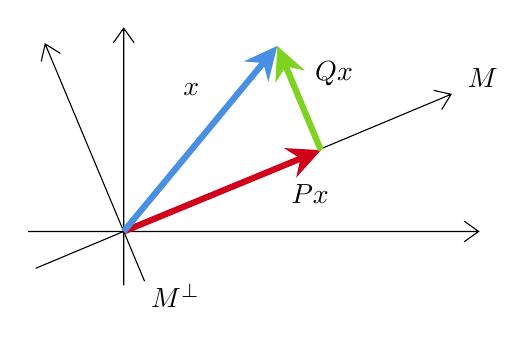
\begin{tikzpicture}[x = 0.75pt, y = 0.75pt, yscale = - 1, xscale = 1]
%uncomment if require: \path (0, 184); %set diagram left start at 0, and has height of 184

%Shape: Axis 2D [id: dp7134109691601231]
\draw (198, 127.91) - - (415, 127.91)(244, 30) - - (244, 153.91) (408, 122.91) - - (415, 127.91) - - (408, 132.91) (239, 37) - - (244, 30) - - (249, 37);
%Shape: Axis 2D [id: dp2976528104012621]
\draw (201.57, 145.68) - - (401.72, 61.83)(206.17, 37.6) - - (254.05, 151.89) (393.33, 59.93) - - (401.72, 61.83) - - (397.2, 69.15) (204.26, 45.99) - - (206.17, 37.6) - - (213.49, 42.13);
%Straight Lines [id: da6603280695196603]
\draw [color = {rgb, 255: red, 208; green, 2; blue, 27}, draw opacity = 1][line width = 2.25] (244, 127.91) - - (334.38, 90.66);
\draw [shift = {(339, 88.75)}, rotate = 517.6] [fill = {rgb, 255: red, 208; green, 2; blue, 27}, fill opacity = 1][line width = 0.08] [draw opacity = 0] (16.07, - 7.72) - - (0, 0) - - (16.07, 7.72) - - (10.67, 0) - - cycle;
%Straight Lines [id: da12421560052711267]
\draw [color = {rgb, 255: red, 74; green, 144; blue, 226}, draw opacity = 1][line width = 2.25] (244, 127.91) - - (314.81, 42.38);
\draw [shift = {(318, 38.53)}, rotate = 489.62] [fill = {rgb, 255: red, 74; green, 144; blue, 226}, fill opacity = 1][line width = 0.08] [draw opacity = 0] (16.07, - 7.72) - - (0, 0) - - (16.07, 7.72) - - (10.67, 0) - - cycle;
%Straight Lines [id: da9584665613249306]
\draw [color = {rgb, 255: red, 126; green, 211; blue, 33}, draw opacity = 1][line width = 2.25] (339, 88.75) - - (319.93, 43.15);
\draw [shift = {(318, 38.53)}, rotate = 427.31] [fill = {rgb, 255: red, 126; green, 211; blue, 33}, fill opacity = 1][line width = 0.08] [draw opacity = 0] (16.07, - 7.72) - - (0, 0) - - (16.07, 7.72) - - (10.67, 0) - - cycle;

% Text Node
\draw (408.5, 48.4) node [anchor = north west][inner sep = 0.75pt] {$M$};
% Text Node
\draw (256, 151.9) node [anchor = north west][inner sep = 0.75pt] {$M^{\perp}$};
% Text Node
\draw (271.5, 55.4) node [anchor = north west][inner sep = 0.75pt] {$x$};
% Text Node
\draw (335, 44.9) node [anchor = north west][inner sep = 0.75pt] {$Qx$};
% Text Node
\draw (323.5, 103.9) node [anchor = north west][inner sep = 0.75pt] {$Px$};
\end{tikzpicture}
\end{figure}
\FloatBarrier

\newpage


\section{Basi hilbertiane e serie di Fourier generalizzata}

\begin{defn}
Sia $H$ uno spazio di Hilbert, $\dim H=+\infty$. Sia $\{e_n\}_{n=1,2,\dots}\subset H$ una successione di vettori di $H$. Si dice che $\{e_n\}$ genera $H$ se $\forall x\in H$ e $\forall\Ec>0$ esiste una successione $\{\lambda_n\}_{n=1,\dots,N}$ tale che
$$
\left\|x-\sum_{n=1}^N\lambda_ne_n \right\|<\Ec
$$
\end{defn}
Ciò significa che è possibile generare uno spazio di dimensione \underline{infinita} con una combinazione lineare \underline{finita} di $\{e_n\}$, attraverso una \textit{tanto buona quanto si vuole} approssimazione.

\begin{rem}
Definendo le somme parziali della serie con $S_N=\sum_{n=1}^N\lambda_ne_n$ si può tradurre la relazione soprastante in 
$$
\lim_{N\to+\infty}S_N=x
$$
dove però è andato perduto il senso di convergenza in norma.
\end{rem}

\begin{defn}
[Base hilbertiana]
Sia $H$ uno spazio di Hilbert, $\dim H=+\infty$. Una successione di vettori $\{e_n\}_{n=1,2,\dots}\subset H$ si dice base hilbertiana, o sistema ortonormale completo, se $\{e_n\}$ genera $H$ ed è ortonormale, ovvero
$$
(e_n,e_m)=\delta_{nm}=
\begin{cases}
0 &m\neq n \\ 1 &m=n
\end{cases} \qquad \qquad \Vert e_n \Vert =1\ \ \forall n
$$
\end{defn}

Osserviamo due cose:
\begin{enumerate}
    \item Non essendo finita, una base hilbertiana non è una base nel senso dell'algebra lineare, ma è la cosa che più le si avvicina in dimensione infinita.
    \item La condizione $\Vert e_n \Vert =1$ è già implicita in $(e_n,e_m)=\delta_{nm}$.
\end{enumerate}

Se avessimo un generico spazio vettoriale $X$ finito potremmo scrivere
$$
x=\sum_{n=1}^Nc_ne_n
$$
e se la base fosse otronormale potremmo addirittura calcolare i coefficienti della combinazione lineare tramite il prodotto scalare
$$
(x,e_n)=\left(\sum_{n=1}^Nc_ne_n,e_n\right)=\sum_{n=1}^Nc_n(e_n,e_n)=c_n
$$
Con una base hilbertiana vale un qualcosa di \textit{mooolto} simile:
\begin{thm}
\label{teoHNOsepa}
Sia $H$ uno spazio di Hilbert, $\dim H=+\infty$. Sia $\{e_n\}_{n=1,2,\dots}\subset H$ una base hilbertiana. Allora un qualsiasi $x\in H$ si scrive come \textbf{serie di Fourier generalizzata}
\begin{equation*}
\boxed{x = \sum^{+\infty}_{n = 1}(x, e_{n}) e_{n}}
\end{equation*}
I coefficienti $(x,e_n)=:\lambda_n$ della combinazione sono detti \textbf{coefficienti di Fourier} di $x$ rispetto $\{e_n\}$, e come nel caso finito sono dati da un prodotto scalare.
\end{thm}

Riprendendo il discorso di inizio pagina, abbiamo che la serie di Fourier generalizzata converge se e solo se
$$
\forall\Ec>0 \quad \exists N\in \NN \quad \text{t.c.}\quad \left\|x-\sum_{n=1}^N(x,e_n)e_n\right\|\leq \Ec
$$

\newpage

\section{Serie di Fourier elementare}

In questo paragrafo si parlerà di funzioni misurabili secondo Lebesgue, cosa che verrà ampiamente approfondita nel prossimo capitolo.

\begin{defn}
Lo spazio delle funzioni a quadrato integrabile è
$$L^2\left([a,b]\right):=\left\{f:[a,b]\to\RR\text{ Lebesgue misurabili t.c. }\displaystyle\int_a^bf^2(x)\dx<+\infty \right\}$$
ed è uno spazio vettoriale.
\end{defn}
Su $L^2$ introduciamo la funzione prodotto scalare
\begin{equation*}
(f,g)=\int_a^bf(x)g(x)\dx
\end{equation*}
e la funzione norma
\begin{equation*}
\Vert f \Vert ^2=\int_a^bf^2(x)\dx=(f,f)
\end{equation*}
in modo tale che $L^2$ sia uno spazio di Hilbert.

Consideriamo ora come spazio di lavoro $L^{2}([ - \pi, \pi])$ e la base
\begin{equation*}
\Bc = \left\{\frac{1}{\sqrt{2\pi}}, \frac{\cos x}{\sqrt{\pi}}, \frac{\sin x}{\sqrt{\pi}}, \frac{\cos2x}{\sqrt{\pi}}, \frac{\sin2x}{\sqrt{\pi}}, \dotsc, \frac{\cos kx}{\sqrt{\pi}}, \frac{\sin kx}{\sqrt{\pi}}, \dotsc  \right\}
\end{equation*}

Si può dimostrare che $\Bc$ è una base hilbertiana secondo il prodotto scalare definito qui sopra.

Allora vale il teorema della serie di Fourier generalizzata, cioè
possiamo costruire ogni funzione $f$ dello spazio di Hilbert $L^2\left([-\pi,\pi]\right)$ tramite la base $\Bc$ come 
\begin{equation*}
\boxed{f(x)=\frac{a_0}{\sqrt{2\pi}}+\sum_{k=1}^{+\infty}\left(a_k\,\frac{\cos kx}{\sqrt{\pi}}+b_k\,\frac{\sin kx}{\sqrt{\pi}}\right)}
\end{equation*}
Questa è la cosiddetta \textbf{serie di Fourier} (elementare) di coefficienti
\begin{equation*}
a_{k} =\left(f,\frac{\cos kx}{\sqrt{\pi}}\right) = \frac{1}{\sqrt{\pi}}\int^{\pi}_{- \pi} f(x)\cos(kx) \dx\qquad
b_{k} = \left(f,\frac{\sin kx}{\sqrt{\pi}}\right) = \frac{1}{\sqrt{\pi}}\int^{\pi}_{- \pi} f(x)\sin(kx) \dx
\end{equation*}

Come per la serie di Fourier generalizzata, anche quella elementare converge se e solo se
$$
\forall\Ec>0 \quad \exists N\in \NN \quad \text{t.c.}\quad \left\|f(x)-\left[\frac{a_0}{\sqrt{2\pi}}+\sum_{k=1}^{+\infty}\left(a_k\,\frac{\cos kx}{\sqrt{\pi}}+b_k\,\frac{\sin kx}{\sqrt{\pi}}\right)\right]\right\|\leq \Ec
$$

Per concludere, è bene notare che con una piccola modifica alla base
\begin{equation*}
\Bc = \left\{\frac{1}{\sqrt{2}}, \cos x, \sin x, \cos 2x, \sin 2x, \dotsc,\cos kx,\sin kx,\dotsc \right\}
\end{equation*}
e al prodotto scalare
\begin{equation*}
(f,g):=\frac{1}{\pi}\int_{-\pi}^\pi f(x)g(x)\dx \qquad \Vert f\Vert^2=\frac{1}{\pi}\int_{-\pi}^\pi f^2(x)\dx
\end{equation*}
si ottiene
\begin{gather*}
\boxed{f(x)=\frac{a_0}{2}+\sum_{k=1}^{+\infty}\left(a_k\cos kx+b_k\sin kx\right)} \\
a_{k} = (f, \cos kx) = \frac{1}{\pi}\int^{\pi}_{- \pi} f(x)\cos(kx) \dx\qquad
b_{k} = (f, \sin kx) = \frac{1}{\pi}\int^{\pi}_{- \pi} f(x)\sin(kx) \dx
\end{gather*}

\newpage

\section{Spazi separabili}

In questa sezione cercheremo di capire se, dato uno spazio di Hilbert generico, esiste una base hilbertiana. Per fare ciò riprendiamo le nozioni di numerabilità e di densità:

\begin{defn}[Insieme numerabile]
Si dice che l'insieme $A$ è numerabile se può essere messo in corrispondenza biunivoca con $\NN$.
\end{defn}
In pratica significa che possiamo \textit{mettere in fila} i suoi elementi:$A=\{a_1,a_2,a_3,\dots\}$.
\begin{defn}[Spazio denso]
Sia $X$ uno spazio normato e siano $A\subseteq B\subseteq X$. Si dice che $A$ è denso in $B$ se $\overline{A}=B$.
\end{defn}
In pratica significa che possiamo sempre costruire una successione in $V$ che approssima, nel senso della norma, lo spazio $H$.
\begin{exa}
$\RR$ non è numerabile. $\QQ$ è denso in $\RR$.
\end{exa}

Siamo pronti:

\begin{defn}[Spazio separabile]
Uno spazio $H$ di Hilbert si dice separabile se ammette un sottoinsieme denso e numerabile, ovvero se $\exists\,V\subset H$ numerabile tale che $\overline{V}=H$.
\end{defn}

\begin{thm}
Uno spazio $H$ di Hilbert, $\dim H=+\infty$, ammette una base hilbertiana se e solo se $H$ è separabile.
\end{thm}

\begin{proof}\leavevmode
\begin{enumerate}
    \item [($\Rightarrow$)] Sia $\{e_n\}$ la base hilbertiana di $H$. Allora la somma parziale $S_N$ è numerabile e approssima nel senso della norma $x\in H$, per cui $H$ è separabile.
    \item [($\Leftarrow$)] Sia $V\subset H$ denso e numerabile. Allora è possibile costruire una base hilbertiana di $H$ usando l'\textbf{algoritmo di ortogonalizzazione di Gram-Schmidt}:
    \begin{align*}
    V&=\left\{x_1,x_2,x_3,\dots \right\} \\
    e_1&=\frac{x_1}{\Vert x_1 \Vert} \\
    e_2&=\frac{x_2-(x_2,e_1)e_1}{\Vert x_2-(x_2,e_1)e_1 \Vert} \\
    e_3&=\frac{x_3-(x_3,e_1)e_1-(x_3,e_2)e_2}{\Vert x_3-(x_3,e_1)e_1-(x_3,e_2)e_2 \Vert} \\
    &\ \vdots
    \end{align*}
    Infatti i vettori $e_n$ sono ortogonali tra loro e hanno norma unitaria per costruzione; inoltre, essendo $V$ denso, generano $H$.
\end{enumerate}
\end{proof}

\newpage

\section{Serie di Fourier generalizzate su spazi separabili}

Ora riprendiamo a parlare di serie di Fourier generalizzate.

Grazie alla nozione di spazio di Hilbert separabile possiamo re-interpretare il teorema (\ref{teoHNOsepa}): è possibile sostituire all'ipotesi di esistenza della base hilbertiana $\{e_n\}$ la separabilità dello spazio di Hilbert considerato.

In ogni caso, una volta che sappiamo che esiste $\{e_n\}$ (che sia diretta conseguenza della separabilità oppure un'ipotesi) ha senso la seguente
$$
\Vert x\Vert^2=\sum_{n=1}^{+\infty} (x,e_n)^2 \qquad\qquad  \textbf{identità di Parseval}
$$
dove si ricorda che $(x,e_n):=\lambda_n$ sono i coefficienti di Fourier di $x$ rispetto la base $\{e_n\}$. Tale identità è banalmente verificabile:
\begin{align*}
\Vert x \Vert^2&=(x,x)=\left(\sum_{n=1}^{+\infty}(x,e_n)e_n,\sum_{k=1}^{+\infty}(x,e_k)e_k\right)=\\
&=\sum_{n=1}^{+\infty}\sum_{k=1}^{+\infty} (x,e_n)(x,e_k)\underbrace{(e_n,e_k)}_{\delta_{nk}}=\sum_{n=1}^{+\infty} (x,e_n)^2
\end{align*}

L'identità di Parseval permette di dire che la successione $\{\lambda_n\}$ dei coefficienti di Fourier è una successione a quadrato sommabile, ovvero $\{\lambda_n\}\subset \ell^2$ (se si parla di serie di Fourier elementare si ha $\{a_n\},\ \{b_n\}\in\ell^2$).

In realtà Parseval suggerisce qualcosa in più: è possibile definire un'applicazione $L:H\to\ell^2$ che associa ad ogni $x\in H$ la successione $\lambda=\{\lambda_n\}=\{(x,e_n)\}\subset\ell^2$ dei suoi coefficienti di Fourier rispetto alla base $\{e_n\}$; tale applicazione è ovviamente \underline{lineare}
$$
(ax+by,e_n)=a(x,e_n)+b(y,e_n)
$$
\underline{isometrica} (stessa metrica su dominio e codominio)
$$
\Vert Lx \Vert_{\ell^2}=\Vert \lambda \Vert_{\ell^2}=\left(\sum_{n=1}^{+\infty}\lambda_n^2\right)^{1/2} =\Vert x \Vert_H
$$
e di conseguenza anche \underline{iniettiva} e \underline{continua}. 

Tutto questo, in \textit{matematichese}, si traduce in
\begin{thm}
Sia $H$ uno spazio di Hilbert separabile di dimensione infinita. Allora $H$ è isomorfo e isometrico allo spazio $\ell^2$, cioè esiste un \textbf{isomorfismo isometrico}
\begin{align*}
L:H&\to\ell^2 \\
x&\mapsto Lx=\{(x,e_n)\}
\end{align*}
\end{thm} 

\begin{proof}
Per dimostrare l'asserto dobbiamo dimostrare che $H$ e $\ell^2$ sono isometrici, cioè sono dotati della stessa metrica, e isomorfi, cioè $L$ è una mappa lineare continua e biunivoca.

Ma che i due spazi sono isometrici
\begin{equation*}
\Vert Lx \Vert_{\ell^2}=\Vert x \Vert_H \qquad \forall x\in H
\end{equation*}
e che $L$ è lineare continua e iniettiva l'avevamo già dedotto dall'identità di Parseval.

Dunque l'unica cosa che veramente viene aggiunta da questo teorema è la \underline{suriettività} di $L$: per dimostrare quest'ultima bisogna prendere $a=(a_1,a_2,\dots)\in\ell^2$ e verificare che $Lx=a$. 

Consideriamo allora la somma parziale
$$
x_n:=\sum_{k=1}^na_ke_k
$$
Sappiamo due cose: che $\sum_{k=1}^\infty a_k^2$ converge (per definizione di $\ell^2$) e che gli $e_k$ sono ortonormali (per definizione di base hilbertiana). Da ciò si deduce che per ogni $\Ec>0$ esiste $N\in \NN$ tale che per ogni $n>m>N$
$$
\Vert x_n-x_m\Vert_H^2=\left\|\sum_{k=m+1}^n a_ke_k\right\|^2=\sum_{k=m+1}^n a_k^2<\Ec
$$
Pertanto la successione $\{x_n\}$ è di Cauchy in $H$ ed essendo quest'ultimo completo esiste $x\in H$ tale che $x_n\to x$. Si verifica immediatamente che i coefficienti di Fourier di $x$ coincidono con gli $a_k$ e quindi $Lx=a$: $L$ è suriettiva.
\end{proof}

\begin{rem}
Tale teorema è l'estensione infinito-dimensionale al teorema che mette in corrispondenza un insieme qualsiasi di dimensione $n$ a $\RR^n$.
\end{rem}


\section{Convergenza, continuità e derivabilità della serie di Fourier elementare}

Studiamo in maniera più approfondita lo spazio di Hilbert separabile $L^2([-\pi,\pi])$ con il prodotto scalare definito da
\begin{equation*}
(f,g)_{L^2}:=\frac{1}{\pi} \int_{-\pi}^\pi fg\qquad \forall f,g\in L^2([-\pi,\pi])
\end{equation*}
e con la norma indotta
\begin{equation*}
\Vert f\Vert_{L^2}^2=\frac{1}{\pi} \int_{-\pi}^\pi f^2\qquad \forall f\in L^2([-\pi,\pi])
\end{equation*}
Consideriamo poi l'insieme (numerabile) di funzioni
\begin{equation*}
\Bc = \left\{\frac{1}{\sqrt{2}}, \cos x, \sin x, \cos 2x, \sin 2x, \dotsc,\cos kx,\sin kx,\dotsc \right\}
\end{equation*}
Si può dimostrare che tale base è hilbertiana in $L^2([-\pi,\pi])$ rispetto al prodotto scalare sopra definito, perciò data una qualunque funzione $f\in L^2([-\pi,\pi])$ è sempre possibile determinare due successioni reali $\{a_n\}$ e $\{b_n\}$ tali che
\begin{equation*}
\boxed{f(x)=\frac{a_0}{2}+\sum_{k=1}^{+\infty}\left(a_k\cos kx+b_k\sin kx\right)}
\end{equation*}
dove
\begin{align*}
a_{k} &= (f, \cos kx) = \frac{1}{\pi}\int^{\pi}_{- \pi} f(x)\cos(kx) \dx\\
b_{k} &= (f, \sin kx) = \frac{1}{\pi}\int^{\pi}_{- \pi} f(x)\sin(kx) \dx
\end{align*}
Analogamente a quanto avevamo già detto, la serie di Fourier elementare converge in $L^2$ se e solo se 
$$
\forall\Ec>0 \quad \exists N\in \NN \quad \text{t.c.}\quad \left\|f(x)-\left[\frac{a_0}{2}+\sum_{k=1}^{+\infty}\left(a_k\cos kx+b_k\sin kx\right)\right]\right\|\leq \Ec
$$
il che equivale a dire che $\{S_N\}$ \textbf{converge in media quadratica} a $f$
\begin{equation*}
\lim\limits_{N\rightarrow + \infty}\left[\int^{\pi}_{- \pi}\left[f(x) - S_{N}(x)\right]^{2} \dx\right] = 0 \qquad \text{con}\qquad S_{N}(x) = \frac{a_{0}}{2} + \sum\limits^{N}_{n = 1}\left(a_n\cos nx+b_n\sin nx\right)
\end{equation*}
Inoltre, l'identità di Parseval diventa 
$$
\Vert f \Vert_{L^2}^2=\pi\left\{\frac{a_0^2}{2}+\sum_{k=1}^{+\infty}\left(a_k^2+b_k^2\right)\right\}
$$
che sembra un po' l'estensione infinito-dimensionale del teorema di Pitagora.

\begin{rem}
Quanto sopra descritto è possibile solamente nel caso in cui la funzione $f\in L^2$ sia periodica di periodo $2\pi$, anche si può chiaramente generalizzare il risultato a periodi generici $T$
\begin{equation*}
f(x) = \frac{a_{0}}{2} + \sum\limits^{\infty}_{n = 1}\left[a_{n}\cos\left(\frac{2n\pi}{T} x\right) + b_{n}\sin\left(\frac{2n\pi}{T} x\right)\right] \qquad \forall f\in L^{2}\left(\left[ - \frac{T}{2}, \frac{T}{2}\right]\right)
\end{equation*}
con prodotto scalare
\begin{equation*}
(f, g) = \frac{2}{T}\int^{T/2}_{- T/2} f(x) g(x) \dx
\end{equation*}
e quindi
\begin{align*}
a_{n} &= \frac{2}{T}\int^{T/2}_{- T/2} f(x)\cos\left(\frac{2n\pi}{T} x\right) \dx \\
b_{n} &= \frac{2}{T}\int^{T/2}_{- T/2} f(x)\sin\left(\frac{2n\pi}{T} x\right) \dx
\end{align*}
Osserviamo però che il calcolo dei coefficenti $a_,b_n$ è possibile nella sola ipotesi in cui $f$ sia solamente integrabile, ovvero $f\in L^1$; tuttavia in questo spazio vengono a mancare sia l'identità di Parseval che particolari proprietà di convergenza (calma, ora le vediamo), che sono invece presenti nello spazio più piccolo $L^2$.
\end{rem}

\subsection{Sulla continuità}

Vediamo ora altri tipi di convergenza delle serie di Fourier.

\begin{thm}[Criterio di Dirichlet]
Se $a_n,b_n\downarrow0$, cioè le successioni decrescono monotamente a 0 e sono positive, allora la serie di Fourier $f(x)$ converge puntualmente in $[-\pi,\pi]$.
\end{thm}

\begin{thm}[Criterio di Weierstrass]
Se $\displaystyle\sum_{k=1}^{+\infty}\left(|a_k|+|b_k|\right)<+\infty$ allora la serie di Fourier $f(x)$ converge uniformemente in $[-\pi,\pi]$.
\end{thm}
\begin{proof}
Posto 
$$
c_k=\sup_{x\in[-\pi,\pi]} |a_k\cos kx+b_k\sin kx|
$$
si ha
$$
\sum_{k=1}^{+\infty} c_k \leq \sum_{k=1}^{+\infty} |a_k+b_k| \leq \sum_{k=1}^{+\infty}\left(|a_k|+|b_k|\right)<+\infty 
$$
e quindi la serie di Fourier converge uniformemente.
\end{proof}

\begin{thm}[Continuità]
Se la serie di Fourier $f(x)$ converge uniformemente in $[-\pi,\pi]$ allora $f\in\Cc^0\left([-\pi,\pi]\right)$ e in particolare $f(-\pi)=f(\pi)$; inoltre, per la periodicità della funzione, si ha continuità in tutto $\RR$.
\end{thm}

Vi sono tuttavia diversi risultati che garantiscono direttamente la convergenza puntuale senza coinvolgere la convergenza uniforme o il criterio di Dirichlet. Vediamone uno in particolare.

\begin{defn}[Funzione regolare a tratti]
Una funzione $f: [-\pi, \pi]\rightarrow \RR$ si dice regolare a tratti se $f$ è limitata in $[-\pi, \pi]$ e l'intervallo si può scomporre in un numero finito di sottointervalli su ciascuno dei quali $f$ è continua e derivabile; inoltre agli estremi di ogni sottointervallo, esistono finiti i limiti sia di $f$ che di $f'$.
\end{defn}

Tale classe di funzioni è molto ampia, perché ci possono essere dei punti angolosi e persino delle discontinuità di tipo salto; sono però escluse funzioni con asintoti verticali o punti a tangenza verticale.

\begin{thm}
[Convergenza puntuale per funzioni regolari a tratti]
Sia $f: [ - \pi, \pi]\rightarrow \RR$ regolare a tratti. Allora la serie di Fourier associata a $f$ converge in ogni punto $x_0\in [ - \pi, \pi]$ alla media dei limiti destro e sinistro:
$$
f(x_0)=\frac{a_0}{2}+\sum_{n=1}^{+\infty}\left(a_n\cos nx_0+b_n\sin nx_0\right)=\frac{f(x_0^+)+f(x_0^-)}{2}
$$
In particolare, se $f$ è continua in $x_0$, allora la serie di Fourier converge a $f(x_0)$.
\end{thm}

\subsection{Sulla derivazione}

Osserviamo che derivando la serie di Fourier si ottiene
\begin{equation*}
f'(x) = \sum\limits^{\infty}_{n = 1}a_nn(-\sin nx)+b_nn\cos nx
\end{equation*}
che converge uniformemente, e quindi $f\in\Cc^1(\RR)$, se
\begin{equation*}
\sum\limits^{\infty}_{n = 1} n(| a_{n}| + | b_{n}|) < \infty
\end{equation*} 
Iterando il ragionamento otteniamo il seguente
\begin{thm}[Derivabilità]
$f\in\Cc^k(\RR)$ se
\begin{equation*}
\sum\limits^{\infty}_{n = 1} n^{k}(| a_{n}| + | b_{n}|) < \infty
\end{equation*}
\end{thm}

Ad ogni derivazione la serie diventa ``meno infinitesima'' a causa della moltiplicazione per $n$; questo significa che ad una maggiore velocità di decadimento dei coefficienti corrisponde una maggiore regolarità della serie.

\begin{exa}
La serie trigonometrica
$$
\sum_{n=1}^{+\infty}\left(\frac{\cos nx}{n^2}+\frac{\sin nx}{n^2}\right)
$$
converge uniformemente. Derivando tale serie otteniamo
$$
\sum_{n=1}^{+\infty}\left(\frac{\cos nx}{n}-\frac{\sin nx}{n}\right)
$$
e ci accorgiamo che la situazione è ``peggiorata''.
\end{exa}
Possiamo concludere che, a differenza delle serie di potenze, le serie di Fourier possono perdere la convergenza dopo una derivazione; questo però non è del tutto a loro sfavore: infatti non ha senso usare una serie di potenze per approssimare una funzione che non è $\Cc^{\infty}$, ma ha perfettamente senso farlo con una serie di Fourier.

Concludiamo con 
\begin{thm}
Se i coefficienti della serie di Fourier decrescono esponenzialmente, ovvero 
$$
|a_k|+|b_k|\leq c_1e^{-c_2k} \qquad \qquad c_1,c_2>0
$$
allora $f\in\Cc^\infty$.
\end{thm}

\subsection{Forma esponenziale delle serie di Fourier}

La ben nota formula di Eulero per l'esponenziale di un immaginario puro, $e^{i\theta}=\cos\theta+i\sin\theta$, suggerisce di scrivere una serie di Fourier utilizzando gli esponenziali.

Ricaviamo
\begin{equation*}
\cos(nx) = \frac{e^{inx} + e^{- inx}}{2}\qquad \qquad \sin(nx) = \frac{e^{inx} - e^{- inx}}{2i}
\end{equation*}
e dunque ponendo
\begin{equation*}
c_n=\frac{a_n-ib_n}{2}\qquad \qquad c_{-n}=\frac{a_n+ib_n}{2}=\overline{c_n}
\end{equation*}
si ottiene la \textbf{forma esponenziale} della serie di Fourier
\begin{equation*}
\boxed{f(x) = \sum\limits_{n\in\ZZ} c_{n} e^{inx}}
\end{equation*}
dove l'uguaglianza è da intendersi come convergenza in $L^2$ delle somme parziali rispetto alla norma indotta dal prodotto scalare
$$
(f, g) = \frac{1}{2\pi}\int^{\pi}_{- \pi} f(x)\,\overline{g(x)} \dx
$$
Come per la serie di seni e coseni, i coefficienti di Fourier si calcolano con il prodotto scalare
\begin{align*}
c_{n} &=\frac{a_n-ib_n}{2}=\frac{1}{2\pi}\int^{\pi}_{- \pi} f(x)\, e^{- inx} \dx \\
c_{-n} &=\frac{a_n+ib_n}{2} =\frac{1}{2\pi}\int^{\pi}_{- \pi} f(x)\, e^{ inx} \dx
\end{align*}
dove si è presa la base ortonormale (si può dimostrare che è anche hilbertiana)
$$
\left\{\frac{e^{inx}}{\sqrt{2\pi}}  \right\}_{n\in\ZZ}
$$
Inoltre, si ha $a_n=c_n+c_{-n}$ e $b_n=i(c_n-c_{-n})$ e l'identità di Parseval assomiglia sempre di più al teorema di Pitagora:
$$
\frac{1}{2\pi}\int^{\pi}_{- \pi} f^2(x) \dx =\sum_{n\in\ZZ} c_n^2
$$
\begin{rem}
Esistono tante altre basi ortonormali (hilbertiane) che permettono di riscrivere a piacere la serie di Fourier elementare: la base di Legendre, Chebychev, Bessel, ecc. Ecco che capiamo perché si è voluto generalizzare il concetto di serie di Fourier elementare con il concetto di serie di Fourier generalizzata!
\end{rem}


\chapter{Integrale di Lebesgue e spazi \texorpdfstring{$L^p$}{C}}

La teoria dell'integrazione di Lebesgue è un importante strumento nelle applicazioni ed è quindi necessario averne una buona conoscenza. In questo capitolo richiameremo le definizioni di base e i principali risultati.\\
Se confrontata con la più intuitiva teoria dell'integrazione secondo Riemann, la teoria dell'integrazione secondo Lebesgue introduce una più ampia classe di funzioni integrabili; tale ampliamento del concetto di integrabilità fa sì che lo spazio $L^1$ delle funzioni integrabili secondo Lebesgue acquisisca la struttura di spazio di Banach, che può essere estesa in genere a tutti gli spazi $L^p$.

\section{Integrale di Riemann (accenni)}

Ricordiamo dal corso di AN1 che, dette 
\begin{align*}
S(\Pc)&=\text{somma superiore}\\
s(\Pc)&=\text{somma inferiore}
\end{align*}
e
\begin{align*}
S&=\inf_{\Pc}S(\Pc) \\
s&=\sup_{\Pc}s(\Pc)
\end{align*}
la funzione $f:[a,b]\to\RR$ è Riemann-integrabile se e solo se $s=S$, e in particolare l'integrale definito di Riemann di $f$ in $x$ è
\begin{equation*}
s=S=:\int_{a}^{b}f(x)\dx
\end{equation*}
Come possiamo vedere, la definizione di integrale di Riemann è molto semplice e intuitiva. In pratica, si tratta di approssimare una funzione limitata con due funzioni ``a gradini'' che forniscono due approssimazioni, una per eccesso e una per difetto; se riusciamo ad avere due stime che differiscono per quantità arbitrariamente piccole diremo che la funzione è integrabile secondo Riemann.

A causa della sua semplicità, il rischio che si corre è quello di non riuscire a integrare funzioni ``strane''. Si consideri per esempio la funzione di Dirichlet $f$ definita nell'intervallo $[0,1]$ da
\begin{equation*}
f(x):=\begin{cases}
1 &x\in[0,1]\cap\QQ \\
0 &x\in[0,1]\setminus\QQ
\end{cases}
\end{equation*}
Per qualunque suddivisione di $[0,1]$ risulta $S=1$ e $s=0$ quindi $f$ non è integrabile secondo Riemann.

Non ci occupiamo qui di elencare le proprietà dell'integrale di Riemann, e passiamo direttamente a definire l'integrale di Lebesgue.

\section{Integrale di Lebesgue}

\subsection{Misura di Lebesgue}
Chiamiamo \textbf{plurirettangolo} (o plurintervallo) l'unione $P$ di un numero finito di intervalli $[a_i,b_i]$
\begin{equation*}
P\subset \RR^{n}, \ \ P = [a_{1}, b_{1}] \times \dotsc \times [a_{n}, b_{n}]
\end{equation*}
La \textbf{misura} del plurirettangolo viene definita come
\begin{equation*}
|P| = (b_{1} - a_{1}) \dotsc (b_{n} - a_{n})
\end{equation*}

\begin{defn}
Sia $A$ un aperto limitato non vuoto di $\RR^n$; la misura di $A$ è l'estremo superiore delle misure dei plurirettangoli contenuti in $A$:
\begin{equation*}
|A| := \sup \left\{|P|, P\in \text{plurirettangoli}, P\subset A\right\}
\end{equation*}
\end{defn}

\begin{defn}
Sia $C$ un chiuso limitato non vuoto di $\RR^n$; la misura di $C$ è l'estremo inferiore delle misure dei plurirettangoli contenuti in $C$:
\begin{equation*}
| C| := \inf\left\{| P|, P\in \text{plurirettangoli}, P\supset C\right\}
\end{equation*}
\end{defn}

Possiamo ora considerare un generico insieme di $\RR^n$:
\begin{defn}
Sia $E$ un insieme limitato di $\RR^n$. Si definiscono
\begin{itemize}
\item \textbf{misura esterna} di $E$, $| E|^{*} := \inf\left\{| A|, A\ \text{aperto}, A\supseteq E\right\}$
\item \textbf{misura interna} di $E$, $| E|_{*} := \sup \left\{| C|, C\ \text{chiuso}, C\subseteq E\right\}$
\end{itemize}
\end{defn}

\begin{rem}
Se $E$ è aperto o chiuso si ha ovviamente $| E|^{*}=|E|=| E|_{*}$. Inoltre per ogni insieme $E$ limitato risulta $| E|^{*}\geq | E|_{*}$.
\end{rem}

\begin{defn}
\label{Leb_limitato}
Un insieme $E$ si dice misurabile secondo Lebesgue se $| E|^{*} = | E|_{*}$.
\end{defn}
Questo concetto di misurabilità è stato introdotto soltanto per insiemi limitati; tuttavia, nelle applicazioni può essere utile estendere la nozione di misurabilità a insiemi illimitati. A tale scopo, dopo aver osservato che l'intersezione di due insiemi (limitati) misurabili è misurabile, diamo la seguente
\begin{defn}
\label{Leb_illimitato}
Un insieme $E\subseteq\RR^n$ (anche illimitato) è \textbf{misurabile secondo Lebesgue} se per ogni $r>0$ l'insieme $E\cap B_{r}$ è misurabile secondo la definizione (\ref{Leb_limitato}), con $B_r:=\{x\in\RR^n\ :\ |x|<r \}$. In tal caso si definisce
$$
| E| : = \lim\limits_{r\rightarrow + \infty}| E\cap B_{r}| \in[0,+\infty]
$$
\end{defn}
\begin{rem}
Scegliendo $r>0$ abbastanza grande (in modo che $E\cap B_{r}=E$) si deduce che gli insiemi misurabili secondo la definzione (\ref{Leb_limitato}) sono misurabili anche secondo la definizone (\ref{Leb_illimitato}). Abbiamo quindi esteso corretamente il concetto di misurabilità secondo Lebesgue.
\end{rem}
Da ora in poi con misurabilità secondo Lebesgue si intenderà la nozione intodotta dalla definizone (\ref{Leb_illimitato}).

\newpage

\begin{thm}
Sia $\{E_i\}$ una successione di insiemi misurabili di $\RR^n$. Allora l'insieme 
$$
E:=\bigcup_{i=1}^\infty E_i
$$ 
è misurabile e vale la seguente disuguaglianza (subadditività numerabile della misura)
$$
|E|\leq \sum_{i=1}^\infty |E_i|
$$
In particolare, se $E_i\cap E_j=\varnothing$ per ogni $i\neq j$ allora vale l'uguale nella formula (additività numerabile della misura). Inoltre, se supponiamo che la successione $\{E_i\}$ sia non decrescente rispetto all'inclusione, cioè $E_1\subseteq E_2\subseteq\dots$, allora
$$
|E|=\lim_{i\to\infty}|E_i|
$$ 
\end{thm}
\begin{rem}
Usando tale teorema si può dimostare un asserto analogo anche per $\displaystyle\bigcap_{i=1}^\infty E_i$.
\end{rem}
Per comprendere l'importanza di tale teorema si osservi che un insieme formato da un'infinità numerabile di punti ha misura nulla!

All'atto pratico, quasi tutti gli insiemi sono misurabili; quelli non misurabili sono casi piuttosto ``patologici'' (un celebre esempio è quello dovuto a \textit{Vitali}).

\subsection{Funzioni misurabili}

\begin{defn}
Una funzione $f: A\subset \RR^{n}\rightarrow \RR$ è \textbf{misurabile} se per ogni $c\in\RR$ l'insieme
\begin{equation*}
\{x\in A\ :\ f(x) < c\}
\end{equation*}
è misurabile secondo Lebesgue.
\end{defn}

\begin{defn}
Sia $A\subseteq\RR^n$ misurabile e siano $f,g:A\to\RR$ misurabili. Si dice che $f$ è uguale a $g$ \textbf{quasi ovunque} in $A$ se
$$
|\{x\in A\ :\ f(x)\neq g(x)\}|=0
$$
Si dice inoltre che una certa proprietà vale quasi ovunque in $x$ se l'insieme degli $x\in A$ per i quali tale proprietà non vale è un insieme di misura nulla.
\end{defn}

Accenniamo solamente al fatto che da qui possiamo andare a definire le somme inferiori $s$ e superiori $S$ ``alla Lebesgue'' di $f$. Ma quello che ci interessa davvero è il concetto di integrale.

\newpage

\subsection{Integrale di Lebesgue}

Procediamo per passi successivi:
\begin{enumerate}
    \item [(i)] Funzioni misurabili e limitate su insiemi di misura finita.

    \begin{defn}
    Sia $A\subset\RR^n$ di misura finita e $f:A\to\RR$ misurabile e limitata. Allora
    $$
    \sup s = \inf S =:\int_A f(x) \dx
    $$
    viene detto integrale di Lebesgue di $f$ su $A$.
    \end{defn}

    \item [(ii)] Funzioni misurabili nonnegative (non necessariamente limitate) su insiemi di misura finita.

    Sia $A\subseteq\RR^n$ di misura finita e $f:A\to\RR$ misurabile e nonnegativa. Per ogni $\lambda>0$ definiamo
    $$
    f_\lambda(x):=\begin{cases}
    f(x) &f(x)\leq\lambda \\
    \lambda &f(x)>\lambda
    \end{cases}
    $$
    Notiamo che esiste $\int_A f_\lambda(x)\dx$ e che è una funzione crescente di $\lambda$; esiste quindi il limite per $\lambda\to\infty$. Se tale limite è infinito diremo che $f$ non è integrabile su $A$ e scriveremo
    $$
    \int_A f(x)\dx=+\infty
    $$
    Se invece tale limite è finito diremo che $f$ è integrabile su $A$ e porremo
    $$
    \int_A f(x)\dx=\lim_{\lambda\to\infty}\int_A f_\lambda(x) \dx
    $$
    \item [(iii)] Funzioni misurabili nonnegative (non necessariamente limitate) su insiemi misurabili (non necessariamente di misura finita).

    Se per ogni $r>0$ la funzione $f$ è integrabile sull'insieme $A_r=A\cap B_r$ possiamo dire che la funzione $r\mapsto\int_{A_r}f(x)\dx$ è crescente e quindi ammette limite per $r\to\infty$. Se tale limite è infinito diremo che $f$ non è integrabile su $A$ e scriveremo
    $$
    \int_A f(x)\dx=+\infty
    $$
    Se invece tale limite è finito diremo che $f$ è integrabile su $A$ e porremo
    $$
    \int_A f(x)\dx=\lim_{r\to\infty}\int_{A_r} f(x) \dx
    $$

    \item [(iv)] Funzioni misurabili di segno qualunque su insiemi misurabili qualunque.

    \begin{defn}
    Sia $A\subseteq \RR^n$ un insieme misurabile secondo Lebesgue. Si dice che una funzione misurabile $f:A\to\RR$ è integrabile secondo Lebesgue se le funzioni (nonnegative) $f^+:=\max\{f,0\}$ e $f^-:=\min\{f,0\}$ sono integrabili secondo Lebesgue, e si pone
    $$
    \int_A f(x)\dx:=\int_A f^+(x)\dx+\int_A f^-(x)\dx
    $$
    La classe delle funzioni Lebesgue-integrabili su $A$ sarà indicata con $L^1(A)$.
    \end{defn}

    Vale il seguente criterio di integrabilità:
    $$
    f\text{ è integrabile su }A\ \Leftrightarrow\ f^+,f^-\text{ sono integrabili su }A\ \Leftrightarrow\ |f|\text{ è integrabile su }A
    $$
    
\end{enumerate}

Per esempio, la funzione di Dirichlet non è integrabile su $[0,1]$ secondo Riemann, ma il suo integrale di Lebesgue esiste e vale $0$.

\newpage

\subsection{Proprietà dell'integrale di Lebesgue}

Ciò che rende la teoria dell'integrazione di Lebesgue fruttosa è il fatto che l'insieme $L^1$ sia ricco di proprietà.

\begin{thm}
Sia $A\subseteq\RR^n$ un insieme misurabile secondo Lebesgue. Allora valgono le seguenti proprietà: 
\begin{itemize}
    \item \textit{Omogeneità.} Se $f\in L^1(A)$ e $c\in\RR$ allora $cf\in L^1(A)$ e 
    $$
    \int_A cf = c\int_A f
    $$

    \item \textit{Additività rispetto alla funzione integranda.} Se $f,g\in L^1(A)$ anche $f+g\in L^1(A)$ e 
    $$
    \int_A f+g=\int_A f+\int_A g
    $$

    \item \textit{Monotonia.}
    \begin{itemize}
        \item Se $f,g\in L^1(A)$ e $f\leq g$ allora $\int_A f\leq \int_A g$.
        \item Per ogni $f\in L^1(A)$ vale $\left|\int_A f \right|\leq \int_A |f|$.
        \item Se $|f|\leq g$ e $g\in L^1(A)$ allora anche $f\in L^1(A)$.
    \end{itemize}

    \item \textit{Additività numerabile rispetto al dominio di integrazione.} Se $f\in L^1(A)$ e $A$ è unione numerabile di insiemi $A_k$ disgiunti a due a due, allora 
    $$
    \int_A f =\sum_{k=1}^{\infty}\int_{A_k} f
    $$

    \item \textit{Insiemi di misura nulla.} Sia $f\in L^1(A)$
    \begin{itemize}
        \item Se $|A|=0$ allora $\int_A f=0$.
        \item Se $g=f$ q.o. in $A$, anche $g\in L^1(A)$ e $\int_A f=\int_A g$.
        \item Se $f\geq 0$ e $\int_A f=0$ allora $f=0$ q.o. in $A$.    
    \end{itemize}
\end{itemize}
\end{thm}

\begin{thm}[Fubini]$\\$
Sia $A\subseteq\RR^{n+m}$ un insieme misurabile tale che $A=A_1\times A_2$ con $A_1\in\RR^n$ e $A_2\in\RR^m$. Sia $f\in L^{1}(A)$ e prendiamo $x\in A_1$ e $y\in A_2$. Allora
\begin{equation*}
\int_A f(x,y) \dxy = \int_{A_1}\left[\int_{A_2} f(x, y) \dy\right] \dx
\end{equation*}
\end{thm}

\begin{thm}[Convergenza Monotona]$\\$
Sia $f_{n} : A\rightarrow [0, + \infty)$ una successione di funzioni misurabili tale che $f_n(x)\to f(x)$ q.o. in $x$ (convergenza puntuale) e $f_{n+1}(x) \geq f_{n}(x)$ q.o. in $x$ e $\forall n$ (monotona crescente). Allora
\begin{equation*}
\lim\limits_{n\rightarrow \infty}\int_{A} f_{n}(x) \dx = \int_{A}\lim\limits_{n\rightarrow +\infty} f_{n}(x) \dx = \int_{A} f(x) \dx
\end{equation*}
\end{thm}

\begin{thm}[Convergenza Dominata]$\\$
Sia $f_{n} : A\rightarrow \CC$ una successione di funzioni misurabili tale che $f_n(x)\to f(x)$ q.o. in $x$ (convergenza puntuale). Se $\exists g\in L^{1}(A)$ tale che $|f_{n}(x)|\leq g(x)$ q.o. in $x$ e $\forall n$ (esistenza di una dominante), allora $f\in L^1(A)$ e
\begin{equation*}
\lim\limits_{n\rightarrow  \infty}\int_{A} f_{n}(x) \dx = \int_{A}\lim\limits_{n\rightarrow  \infty} f_{n}(x) \dx = \int_{A} f(x) \dx
\end{equation*}
\end{thm}


\section{Spazi \texorpdfstring{$L^p$}{C}}

\begin{defn}
Sia $A\subset \RR^{n}$ misurabile. Sia $1 \leq p < \infty $. Poniamo
\begin{equation*}
L^{p}(A) = \left\{f: A\rightarrow \RR\text{ Lebesgue-misurabili t.c. }\int_{A}| f(x)|^{p} \dx < \infty \right\}
\end{equation*}
e inoltre definiamo la norma $p$
$$
\Vert f \Vert_p:= \left(\int_{A}|f(x)|^{p} \dx\right)^{1/p}
$$
per ogni $f\in L^p(A)$.
\end{defn}

Il caso $p=\infty$ merita una trattazione a parte.

\begin{defn}
Sia $A\subseteq\RR^n$ un insieme misurabile. Per ogni funzione $f:A\to\RR$ misurabile definiamo l'\textbf{estremo superiore essenziale} di $f$ su $A$ come
$$
\esssup_{x\in A} f(x):=\inf\left\{ \alpha\in\RR\ :\ \left|f^{-1}(\alpha,+\infty) \right|=+\infty \right\}
$$
dove con $\left|f^{-1}(\alpha,+\infty) \right|$ si intende la misura della controimmagine di $f(\alpha,+\infty)$.
\end{defn}
In pratica si è rivisitato il concetto di estremo superiore in modo tale che non vengano considerati punti a misura nulla. Per intenderci:
\fg{0.4}{bonfa_18}

\begin{defn}
Sia
\begin{equation*}
L^{\infty}(A) = \left\{f: A\rightarrow \RR\text{ Lebesgue-misurabili t.c. }\esssup_{x\in A} |f(x)|<+ \infty \right\}
\end{equation*}
con norma infinito
\begin{equation*}
\Vert f \Vert_{\infty} := \esssup_{x\in A} |f(x)|
\end{equation*}
per ogni $f\in L^\infty(A)$.
\end{defn}

Osserviamo che $\forall p\in[1,+\infty]$ si ha che:
\begin{enumerate}
    \item [$\triangleright$] $L^p$ è uno spazio lineare.

    \item [$\triangleright$] La norma $p$ è a tutti gli effetti una norma ben definita su $L^p$.

    \item [$\triangleright$] $L^p$ dotato di norma $p$ è uno spazio vettoriale completo (di Banach).

    \item [$\triangleright$] In particolare, lo spazio $L^2$ non solo è di Banach, ma è anche di Hilbert rispetto al prodotto scalare
    $$
    (f,g)_{L^2}:=\int_A f(x) g(x)\dx
    $$

    \item [$\triangleright$] $L^p$ è uno spazio separabile tranne per $p=+\infty$.
\end{enumerate}

\begin{defn}
Siano $x,y\in\RR$ e $t\in[0,1]$. Diremo che
$$
tx+(1-t)y
$$
è una combinazione lineare convessa.

Inoltre, diremo che $f$ è convessa se
$$
f(tx+(1-t)y)\leq t f(x)+(1-t)f(y)
$$
mentre diremo che è concava se
$$
f(tx+(1-t)y)\geq t f(x)+(1-t)f(y)
$$
\end{defn}

\begin{thm}
La funzione logaritmo è concava.
\end{thm}

\begin{rem}
Dal punto di vista geometrico, una funzione è concava se comunque si scelgano le ascisse $x,y$ il segmento congiungente i punti $(x,f(x)),(y,f(y))$ sottosta al grafico della funzione.

\end{rem}

\begin{figure}[!htbp]
\centering
\includegraphics[width=0.3\linewidth]{bonfa_19} $\quad$
\includegraphics[width=0.3\linewidth]{bonfa_20}
\caption{Funzione modulo (convessa) a sinistra e logaritmo (concava) a destra}
\end{figure}
\FloatBarrier


\begin{defn}
Due numeri $p, q \geq 1$ sono \textbf{esponenti coniugati} se $\dfrac{1}{p} + \dfrac{1}{q} = 1$.\\
Tale concetto si estende anche al caso $p=1$ e $q=+\infty$ e viceversa.
\end{defn}

\begin{rem}
Prendendo due esponenti coniugati la concavità della funzione logaritmo può essere espressa come
$$
\log\left(\frac{x}{p}+\frac{y}{q}\right)\geq \frac{\log x}{p}+\frac{\log y}{q}
$$
\end{rem}

\begin{thm}[Disuguaglianza di Young]$\\$
Siano $p, q$ esponenti coniugati. Allora $\forall a, b > 0$ vale
\begin{equation*}
ab\leq\frac{a^{p}}{p} + \frac{b^{q}}{q}
\end{equation*}
\end{thm}

\begin{proof}
La dimostrazione si basa sulle proprietà del logaritmo:
$$
\log(ab)=\log(a)+\log(b)=\frac{\log a^p}{p}+\frac{\log b^q}{q}\leq \log\left(\frac{a^p}{p}+\frac{b^q}{q}\right)
$$
Dato che il logaritmo è una funzione crescente posso semplificarlo e ottenere così la tesi.
\end{proof}

\begin{thm}[Disuguaglianza di Holder]$\\$
Sia $A\subseteq\RR^n$ misurabile e siano $p,q\in[0,+\infty]$ coniugati. Se $f\in L^p(A)$ e $g\in L^q(A)$ allora $fg\in L^1(A)$ e
\begin{equation*}
\int_A | f(x) g(x)| \dx=\Vert fg \Vert_1 \leq \Vert f \Vert_{p}\cdot \Vert g \Vert_{q}
\end{equation*}
\end{thm}

\begin{proof}
Dimostriamo prima l'asserto nel caso $p=1$ e $q=\infty$ (la dimostrazione con $q=1$ e $p=\infty$ è del tutto analoga).

Abbiamo $f\in L^1$ e $g\in L^{\infty}$. Per definizone di norma infinito abbiamo 
$$
|g(x)| \leq \Vert g \Vert_{\infty} \qquad\qquad\text{q.o. in }x
$$
e dunque
$$
\int_A |f(x) g(x)| \dx \leq \Vert g \Vert_{\infty}\cdot \int_A |f(x)| \dx = \Vert g \Vert_{\infty}\cdot \Vert f \Vert_{1}
$$

Possiamo passare a dimostrare l'asserto per due generici $1<p,q<\infty$. 

Per semplicità consideriamo dapprima due funzioni $\widetilde{f}\in L^p$ e $\widetilde{g}\in L^q$ tali che $\Vert \widetilde{f}\Vert_p=1$ e $\Vert \widetilde{g}\Vert_q=1$. In questo modo per la disuguaglianza di Young si ha
\begin{align*}
\int_A | \widetilde{f}(x) \widetilde{g}(x)| \dx&\leq \int_A \left(\frac{|\widetilde{f}(x)|^p}{p}+\frac{|\widetilde{g}(x)|^q}{q} \right)\dx \\
&=\left(\frac{\Vert \widetilde{f}\Vert_p^p}{p}+\frac{\Vert \widetilde{g}\Vert_q^q}{q}\right) \\
&=\frac{1}{p}+\frac{1}{q} \\
&=1\left(=\Vert \widetilde{f}\Vert_p\cdot \Vert \widetilde{g}\Vert_q\right)
\end{align*} 

Ma allora il caso generale (con norme non necessariamente unitarie) è banale da verificare:
\begin{gather*}
f(x)=\frac{\Vert f \Vert_{p}}{\Vert f \Vert_{p}} \cdot f(x)=\frac{f(x)}{\Vert f \Vert_{p}} \cdot \Vert f \Vert_{p} = \widetilde{f}(x)\cdot \Vert f \Vert_{p} \\
g(x)=\frac{\Vert g \Vert_{q}}{\Vert g \Vert_{q}} \cdot g(x)=\frac{g(x)}{\Vert g \Vert_{q}} \cdot \Vert g \Vert_{q} = \widetilde{g}(x)\cdot \Vert g \Vert_{q} \\
\Longrightarrow \int_A | f(x) g(x)| \dx =\Vert f \Vert_{p}\cdot \Vert g \Vert_{q} \cdot \int_A | \widetilde{f}(x) \widetilde{g}(x)| \dx \leq \Vert f \Vert_{p}\cdot \Vert g \Vert_{q}
\end{gather*}
\end{proof}

Conseguenze della disuguaglianza di Holder:
\begin{itemize}
    \item Se $A\subset\RR^n$ è un insieme di misura finita e $1\leq p<q\leq+\infty$ allora vale l'inclusione $L^q(A)\subset L^p(A)$ e inoltre
    $$
    \Vert f \Vert_p\leq |A|^{\frac{1}{p}-\frac{1}{q}}\Vert f\Vert_q \qquad \qquad \forall f\in L^q(A) 
    $$
    \begin{rem}
    L'ipotesi di misura finita è indispensabile: infatti se ad esempio $f\equiv 1$ abbiamo $f\in L^\infty(\RR)$ ma $f\notin L^p(\RR)$ per ogni $1\leq p<\infty$.
    \end{rem}

    \item Se $A\subset\RR^n$ è un insieme di misura finita allora per ogni funzione misurabile $f$ si ha
    $$
    \lim_{p\to\infty}\Vert f\Vert_p=\Vert f\Vert_{\infty}
    $$

    \item Permette di dimostrare che $L^2$ è uno spazio di Hilbert (pensandoci, l'unico espnente coniugato con se stesso è proprio $p=2$).
\end{itemize}

\begin{thm}[Disuguaglianza di Minkowski]$\\$
Siano $p \geq 1, f\in L^{p}, g\in L^{p}$. Allora
\begin{equation*}
(f + g) \in L^{p} \ \ \text{e} \ \ \Vert f + g \Vert_{L^{p}} \leq \Vert f \Vert_{L^{p}} + \Vert g \Vert_{L^{p}}
\end{equation*}
\end{thm}
\begin{proof}
\begin{align*}
\Vert f + g \Vert^{p}_{L^{p}} & = \int | f(x) + g(x)|^{p} dx\\
 & = \int | f(x) + g(x)|^{p - 1}| f(x) + g(x)| dx\\
 & \leq \int \underbrace{| f(x) + g(x)|^{p - 1}}_{A}\underbrace{| f(x)|}_{B} dx + \int \underbrace{| f(x) + g(x)|^{p - 1}}_{C}\underbrace{| g(x)|}_{D} dx
\end{align*}
Consideriamo $h(x) = A$
\begin{equation*}
[h(x)]^{q} = [h(x)]^{\frac{p}{p - 1}} = | f(x) + g(x)|^{p}
\end{equation*}
Sappiamo già, per dimostrazione precedente, che $(f + g) \in L^{p}$, allora $h\in L^{q}$. Usiamo la disuguaglianza di Holder su $A\in L^{q}, B\in L^{p}$ e $C\in L^{q}, D\in L^{p}$. Otteniamo
\begin{align*}
\Vert f + g \Vert^{p}_{L^{p}} & \leq \Vert f \Vert_{L^{p}}\left \Vert \ | f + g|^{p - 1} \ \right \Vert_{L^{q}} + \Vert g \Vert_{L^{p}}\left \Vert \ | f + g|^{p - 1} \ \right \Vert_{L^{q}}
\end{align*}
osserviamo il termine che si presenta due volte
\begin{align*}
\left \Vert \ | f + g|^{p - 1} \ \right \Vert_{L^{q}} & = \left(\int | f(x) + g(x)|^{(p - 1) q} dx\right)^{1/q}\\
 & = \left(\int | f(x) + g(x)|^{p} dx\right)^{1/q}\\
 & = \left(\Vert f + g \Vert^{p}_{L^{p}}\right)^{1/q}\\
 & = \Vert f + g \Vert^{p/q}_{L^{p}}\\
 & = \Vert f + g \Vert^{p - 1}_{L^{p}}
\end{align*}
allora
\begin{gather*}
\Vert f + g \Vert^{p}_{L^{p}} \leq \Vert f \Vert_{L^{p}} \Vert f + g \Vert^{p - 1}_{L^{p}} + \Vert g \Vert_{L^{p}} \Vert f + g \Vert^{p - 1}_{L^{p}}\\
\implies \ \ \Vert f + g \Vert_{L^{p}} \leq \Vert f \Vert_{L^{p}} + \Vert g \Vert_{L^{p}}
\end{gather*}
\end{proof}

%zzzzzzzzzzzzzzzzzzzzzzz

\chapter{Distribuzioni}

\section{Spazi di Banach e spazi duali}

Per arrivare a definirle e vedere a cosa servono dobbiamo fare alcuni passaggi preliminari. Definiamo il concetto di spazio duale. Parliamo di spazio duale non necessariamente, ma specialmente nel contesto degli spazi di Banach.

Supponiamo di avere due spazi di Banach $X, Y$ in modo assolutamente generale, poi ci concentreremo su uno specifico.
\begin{defn}
[Linearità] Possiamo considerare tutte le funzioni lineari da $X$ in $Y$
\begin{equation*}
L: X\rightarrow Y\ \ \ \ L(\alpha x_{1} + \beta x_{2}) = \alpha L(x_{1}) + \beta L(x_{2})
\end{equation*}
\end{defn}
Teniamo presente che quando parliamo di spazi di Banach spesso intendiamo spazi a dimensione infinita, in questo caso certe idee che abbiamo molto naturali e intuitive delle funzioni lineari non valgono necessariemente. In particolare la continuità \textbf{non} è necessariamente garantita in caso di funzioni lineari. In uno spazio di Banach possiamo avere funzioni lineari continue e funzioni lineari non continue.
\begin{defn}
[Continuità] Una funzione è continua se
\begin{equation*}
x_{n}\rightarrow x\ \ \implies \ \ L(x_{n})\rightarrow L(x)
\end{equation*}
\end{defn}
Ricordiamo un'altra definizione non scontata negli spazi a dimensione infinita
\begin{defn}
[Limitatezza]
Una funzione lineare è limitata se
\begin{equation*}
\exists c\ \ \Vert L(x) \Vert \leq c \Vert x \Vert \ \ \forall x\in X
\end{equation*}
\end{defn}
Vale un teorema che collega queste due definizioni.
\begin{thm}
Siano $X, Y$ due spazi di Banach qualsiasi. Una funzione lineare $L: X\rightarrow Y$ è limitata se e solo se è continua.
\end{thm}
Quello che ci interessa è un tipo particolare di funzioni tra spazi di Banach. Il secondo spazio sarà $\RR$, che è esso stesso uno spazio di Banach, è uno spazio lineare dotato di norma (il valore assoluto) e continuo rispetto a questa norma.
\begin{equation*}
L: X\rightarrow \RR \ \ \ \ X\ \text{di Banach}
\end{equation*}
\begin{defn}
Dato uno spazio $X$ di Banach, si dice \textbf{spazio duale} l'insieme di tutte le \underline{funzioni lineari continue} da $X$ in $\RR$. Queste funzioni si chiamano anche \textbf{funzionali}.
\end{defn}
Supponiamo per esempio che $X$ sia $\RR^{n}$, possiamo considerare tutte le funzioni lineari (e quindi continue, essendo $\RR^{n}$ a dimensione finita)
\begin{equation*}
L: \RR^{n}\rightarrow \RR
\end{equation*}
Come possiamo descriverle tutte? Le identifichiamo con il prodotto scalare con un altro vettore. Dato $y\in \RR^{n}$ possiamo definire $L(x) : = (y, x)$. Per esempio il duale di $\RR^{n}$ è $\RR^{n}$ stesso.

La categoria più importante di spazi di Banach che abbiamo visto fin'ora è $L^{p}$, cos'è il suo duale? Abbiamo un modo molto semplice.
\begin{thm}
Se $1 < p < + \infty $, allora il duale di $L^{p}$ è $L^{q}$ dove $q$ è l'esponente coniugato di $p$: $\frac{1}{p} + \frac{1}{q} = 1$.
\end{thm}
Sia $f\in L^{p}$ e $L(f) \in \RR$, possiamo dimostrare che $\forall L$ funzionale lineare su $L^{p}$ esiste una funzione $h\in L^{q}$ tale che $L(f) = \int hf$. Non stiamo specificando in quale dominio stiamo definendo questi spazi. Grazie alla disuguaglianza di Holder otteniamo questo risultato. Non indaghiamo ulteriormente.

Torniamo alla definizione di duale. Una possibile notazione dello spazio duale di $X$ è $X'$. Questo spazio duale è lui stesso uno spazio di Banach. È ovviamente uno spazio vettoriale, ma dobbiamo far vedere che c'è una \textit{norma}. Un elemento del duale è un funzionale $L: X\rightarrow \RR$, questo vuol dire che dato un elemento $x\in X$ allora $L(x) \in \RR$
\begin{equation*}
\Vert L \Vert = \sup_{\Vert x \Vert = 1}| L(x)|
\end{equation*}
È vero che questo è effettivamente un numero reale? Abbiamo detto che il duale è fatto da funzionali lineari continui, ovvero limitati, quindi sicuramente questo estremo superiore è limitato. La definizione di poco fa di funzione limitata era che $\exists c$ tale che $| L(x)| \leq c \Vert x \Vert $, quindi sicuramente questo estremo superiore è minore di $c$. Si tratta di far vedere che è effettivamente una norma, abbiamo allora questo teorema.
\begin{thm}
Sia $X$ spazio di Banach. Allora $X'$ è uno spazio di Banach lui stesso rispetto alla norma
\begin{equation*}
\Vert L \Vert = \sup_{\Vert x \Vert = 1}| L(x)|
\end{equation*}
\end{thm}
\begin{defn}
[Supporto di una funzione]
Supponiamo ora di avere una funzione $f: A\subset \RR^{n}\rightarrow \RR$. Si dice supporto di $f$ l'insieme
\begin{equation*}
\supp f = \overline{\{x\in A, f(x) \neq 0\}}
\end{equation*}
È la chiusura dell'insieme dei punti dove la funzione non si annulla.
\end{defn}
Diamo la definizione di un nuovo spazio vettoriale, se abbiamo $A\subset \RR^{n}$ sappiamo cos'è $L^{p}(A)$.
\begin{defn}
Si dice $L^{p}_{\loc}$ l'insieme delle funzioni $f: A\rightarrow \RR$ tali che $\forall K\subset A$ compatto
\begin{equation*}
\exists \ \ \int_{K}| f|^{p} dx\ \ \text{finito} .
\end{equation*}
\end{defn}
È molto più grande dello spazio $L^{p}$.

\section{Funzioni test e distribuzioni}

Adesso dobbiamo definire un nuovo spazio di funzioni, che non è uno spazio di Banach.
\begin{defn}
[Spazio delle funzioni test]
Sia $A\subset \RR^{n}$ aperto. Chiamiamo funzioni $C^{\infty}$ a supporto compatto, o funzioni test, e lo indichiamo con $\Dc(A)$ l'insieme delle funzioni $f: A\rightarrow \RR$, derivabili infinite volte $f\in C^{\infty}$ e tali che il supporto $\supp f$ è compatto.
\end{defn}
Una funzione in $\Dc(A)$ viene detta \textbf{funzione test}. Queste funzioni sono un insieme estremamente piccolo. Non è banale neanche fare degli esempi in $\Dc(\RR)$. Per esempio
\begin{equation*}
f(x) =
\begin{cases}
e^{\frac{1}{x^{2} - 1}} & | x| < 1\\
0 & | x| \geq 1
\end{cases}
\end{equation*}
Somiglia a una gaussiana, ma fuori da $[ - 1, 1]$ si annulla.

\fg{0.7}{esempioFunzioneD}

Non è banale che sia $C^{\infty}$ nei punti $ - 1, 1$, ma si può dimostrare.

Nessuna funzione elementare appartiene a questo insieme.

Questo insieme non è uno spazio di Banach, se definiamo una norma, non può essere uno spazio di Banach rispetto a quella norma. Nonostante ciò vogliamo definire un concetto di convergenza.

Daremo le prossime definizioni in dimensione $1$ per alleggerire le notazioni.
\begin{defn}
[Convergenza in $\Dc$]Sia $A\subset \RR$ aperto e consideriamo l'insieme $\Dc(A)$, consideriamo una successione di funzioni $\{f_{n}\} \subset \Dc(A)$. Diciamo che $f_{n}\rightarrow f$ in $\Dc(A)$ se
\begin{enumerate}
\item $\exists K\subset A$ compatto tale che il supporto $\supp f_{n} \subset K$, ciascuna funzione è a supporto compatto, ma vogliamo che esista un compatto che contenga i supporti di tutte le funzioni.
\item $\forall k\in \NN$ la derivata di ordine $k$ della successione di funzioni converge alla derivata di ordine $k$ della funzione uniformemente $f^{(k)}_{n}\rightarrow f^{(k)}$.
\end{enumerate}
\end{defn}
Si può dimostrare che non possiamo definire questa convergenza in norma o distanza, motivo per cui l'abbiamo definita noi così. Ora possiamo finalmente arrivare alla definizione di distribuzione.
\begin{defn}
[Distribuzione]
Sia $A\subset \RR$ aperto. Chiamiamo \textbf{distribuzione} in $A$ un funzionale (lineare e continuo) su $\Dc(A)$. Quindi lo spazio delle distribuzione è il suo duale $\Dc'(A)$.
\end{defn}
Stiamo cercando di generalizzare il concetto di funzione.
\begin{thm}
A ogni funzione $u\in L^{1}_{\loc}(A)$ corrisponde una distribuzione in $\Dc'(A)$.

Indichiamo con $(u, f)$ il prodotto di dualità, cioè la distribuzione (funzionale lineare e continuo) associata ad $u$ che agisce sulla funzione test $f$
\begin{equation*}
\boxed{(u, f) = \int_{A} ufdx} \ \ \ \ u\in L^{1}_{\loc}(A) \ \ f\in \Dc(A)
\end{equation*}
\end{thm}
\begin{proof}

Dobbiamo verificare che l'integrale sia ben definito, lineare e continuo (o limitato).
\begin{itemize}
\item \textit{ben definito.} Il supporto di $f$ è un certo insieme $K\subset A$ compatto, quindi si annulla al di fuori di $K$, allora
\begin{equation*}
\int_{A} ufdx = \int_{K} ufdx
\end{equation*}ma $f$ è anche limitata (essendo continua a supporto compatto) e $u\in L^{1}_{\loc}$:
\begin{equation*}
\left| \int_{K} ufdx\right| \leq \sup | f| \left| \int_{K} udx\right| < + \infty
\end{equation*}
\item \textit{lineare}, infatti
\begin{equation*}
(u, c_{1} f_{1} + c_{2} f_{2}) = \int_{A} u(c_{1} f_{1} + c_{2} f_{2}) dx
\end{equation*}per la linearità dell'integrale
\begin{equation*}
\int_{A} u(c_{1} f_{1} + c_{2} f_{2}) dx = c_{1}\int_{A} uf_{1} dx + c_{2}\int_{A} uf_{2} dx = c_{1}(u, f_{1}) + c_{2}(u, f_{2})
\end{equation*}
\item \textit{continuo, o limitato} (sono equivalenti). Per ipotesi $f_{n}\rightarrow f$ in $\Dc(A)$ e $u\in L^{1}_{\loc}$. Allora la convergenza in $\Dc(A)$ garantisce che il supporto di tutte le $f_{n}$ sia contenuto in un compatto $K\subset A$, e inoltre $f_{n}\rightarrow f$ (e le derivate) uniformemente, cioè $ \Vert f_{n} - f \Vert_{\infty}\rightarrow 0$. Per definizione di $L^{1}_{\loc}$ la funzione $u$ ristretta al compatto $K$ è $L^{1}(K)$. Possiamo allora usare la disuguaglianza di Holder con $p = 1, q = \infty $ per far vedere che
\begin{equation*}
\left| \int_{K} u(f_{n} - f) dx\right| \leq \Vert u \Vert_{L^{1}(K)} \Vert f_{n} - f \Vert_{\infty}\rightarrow 0
\end{equation*}allora abbiamo fatto vedere che
\begin{equation*}
\int_{A} u(f_{n} - f) dx\rightarrow 0\ \ \ \ \iff \ \ \ \ \int_{A} uf_{n} dx\rightarrow \int_{A} ufdx
\end{equation*}quindi qualsiasi funzione $L^{1}_{\loc}$ è una distribuzione su quell'insieme.
\end{itemize}
\end{proof}

Si noti che lo spazio $L^{1}_{\loc}$ è molto più grande di $L^{1}$, ad esempio banalmente qualunque polinomio non identicamente nullo non è integrabile su tutto $\RR$, ma è integrabile su qualunque compatto.

Tutte le distribuzioni si possono vedere come associate a una funzione $L^{1}_{\loc}$? No, vediamo un controesempio con la \textbf{delta di Dirac}, che definiamo come distribuzione su $\RR$. Ad ogni funzione $f\in \Dc(\RR)$ e $y\in \RR$ vogliamo associare una distribuzione $\delta_{y} \in \Dc'(\RR)$
\begin{equation*}
\boxed{(\delta_{y}, f) = f(y) \in \RR}
\end{equation*}
\begin{proof}\leavevmode
\begin{itemize}
\item ha valori in $\RR$, $\delta_{y} : \Dc(\RR)\rightarrow \RR$
\item è lineare $(\delta_{y}, c_{1} f_{1} + c_{2} f_{2}) = (c_{1} f_{1} + c_{2} f_{2})(y) = c_{1} f_{1}(y) + c_{2} f_{2}(y)$ che è proprio uguale a $c_{1}(\delta_{y}, f_{1}) + c_{2}(\delta_{y}, f_{2})$
\item è continua. Sia $f_{n}\rightarrow f$, cioè il supporto di tutte le $f_{n}$ è contenuto in $K$ compatto e $f_{n}\rightarrow f$ uniformemente, e quindi anche puntualmente:
\begin{itemize}
\item se $y\notin K$ allora $(\delta_{y}, f_{n}) = 0$ e $(\delta_{y}, f) = 0$
\item se $y\in K$ allora $(\delta_{y}, f_{n}) = f_{n}(y)\rightarrow f(y) = (\delta_{y}, f)$
\end{itemize}

\end{itemize}
\end{proof}
Spesso si scrive
\begin{equation*}
(\delta_{y}, f) = \int_{\RR} \delta_{y}(x) f(x) dx = f(y)
\end{equation*}
La delta di Dirac nasce per estrarre in modo semplice il valore di una funzione in un punto, e da qui si è poi sviluppata la teoria delle distribuzioni. Ad ogni funzione $L^{1}_{\loc}$ si può quindi associare una distribuzione, ma non viceversa, le distribuzioni sono di più.

Un altro modo di interpretare la delta di Dirac è il limite di una gaussiana
\begin{equation*}
f(x) = \frac{1}{\sqrt{2\pi}} e^{- \frac{1}{2} x^{2}} \ \ \ \ \Vert f \Vert_{L^{1}} = 1
\end{equation*}
definiamo
\begin{equation*}
f_{n}(x) = nf(nx)
\end{equation*}
\fg{0.7}{deltaGaussianaLimite}

dove
\begin{equation*}
\Vert f_{n} \Vert_{L^{1}} = \int_{\RR}| f_{n}(x)| dx = \int_{\RR} nf(nx) dx
\end{equation*}
chiamo $y = nx$ allora $dy = ndx$
\begin{equation*}
\int_{\RR} nf(nx) dx = \int_{\RR} f(y) dy = 1
\end{equation*}
Notiamo che
\begin{equation*}
f_{n}(x) = \frac{n}{\sqrt{2\pi}} e^{- \frac{1}{2}(nx)^{2}}\xrightarrow{n\rightarrow \infty} 0\ \ \forall x\neq 0
\end{equation*}
Essendo $L^{1}$, quindi anche $L^{1}_{\loc}$, le possiamo vedere come distribuzioni. Possiamo dimostrare che $\forall \varphi \in \Dc(A)$, $(f_{n}, \varphi)\rightarrow (\delta_{0}, \varphi)$.

Più uno spazio è piccolo e più il suo duale è grande, e viceversa. Lo spazio $\Dc(A)$ è molto piccolo, quindi il duale (lo spazio delle distribuzioni) sarà molto grande, ma pur essendo molto grande, avrà delle proprietà molto forti (derivabilità infinita). \textit{Stiamo cercando capre e cavoli}.

\begin{defn}
[Convergenza di una distribuzione]
Cosa vuol dire avere una successione di distribuzioni $\{\Lambda_{n}\}$ che converge a $\Lambda $ \underline{nel senso delle distribuzioni}? Come prima, se $\forall \varphi \in \Dc(A) \implies (\Lambda_{n}, \varphi)\rightarrow (\Lambda, \varphi)$. La definizione è simmetrica rispetto all'altra.
\end{defn}
Veniamo al supporto. Una distribuzione non ha una variabile, non si annulla come una funzione, non è una funzione.
\begin{defn}
[Supporto di una distribuzione]
Sia $\Lambda \subset \Dc'(A)$. Consideriamo $B\subset A$ e $\varphi \in \Dc(B)$. Supponiamo che $(\Lambda, \varphi) = 0\ \ \forall \varphi $. Questo è il modo per dire che "si annulla", diciamo
\begin{equation*}
\boxed{
\supp \Lambda =
\left(\bigcup_{\substack{B\subset A\\B\text{aperti}}} \{B: (\Lambda, \varphi) = 0, \ \forall \varphi \in \Dc(B)\}\right)^{C}
}
\end{equation*}
\end{defn}

NB. Quando diciamo che a $u\in L^{1}_{\loc}(A)$ corrisponde una distribuzione, diciame che esiste una $\Lambda_{u}$ distribuzione definita come $(\Lambda_{u}, \varphi) = \int_{A} u\varphi $, ma talvolta scriveremo direttamente $u$ con abuso di notazione.
\begin{defn}
[Derivata di una distribuzione]
Sia $\Lambda \in \Dc'(A)$ una distribuzione. Definiamo la sua distribuzione derivata $\Lambda'\in \Dc'(A)$. Per ogni $\varphi \in \Dc(A)$ dobbiamo definire quanto vale $(\Lambda', \varphi)$
\begin{equation*}
\boxed{(\Lambda', \varphi) = - (\Lambda, \varphi')}
\end{equation*}
\end{defn}
Questo somiglia molto all'integrazione per parti (in realtà è molto più che una somiglianza). Controlliamo che sia una distribuzione
\begin{itemize}
\item definita $\Lambda': \Dc(A)\rightarrow \RR$, sì per come è costruita, $\varphi'$ è comunque definito essendo $C^{\infty}$ a supporto compatto
\item lineare:
\begin{equation*}
(\Lambda', a_{1} \varphi_{1} + a_{2} \varphi_{2}) = a_{1}(\Lambda', \varphi_{1}) + a_{2}(\Lambda', \varphi_{2})
\end{equation*}
\item continuo:
\begin{equation*}
\varphi_{k}\rightarrow \varphi \ \ \text{in} \ \Dc(A) \ \ \implies \ \ (\Lambda', \varphi_{k})\rightarrow (\Lambda', \varphi)
\end{equation*}

infatti, dato che $\varphi'_{k}\rightarrow \varphi'$
\begin{gather*}
(\Lambda', \varphi_{k}) = - (\Lambda, \varphi'_{k})\rightarrow - (\Lambda, \varphi') = (\Lambda', \varphi)
\end{gather*}
\end{itemize}

Andiamo ora a capire che ha le stesse proprietà di una derivata. Consideriamo una funzione derivabile $u\in C^{1}(A) \subset L^{1}_{\loc}(A)$, ma allora è associata ad una distribuzione, che continueremo a chiamare $u$
\begin{equation*}
(u, \varphi) = \int_{A} u(x) \varphi (x) dx
\end{equation*}
Sappiamo che esiste $u'\in C^{0}(A) \subset L^{1}_{\loc}$, associata a sua a volta ad una distribuzione
\begin{gather*}
\underbrace{(u', \varphi) = - (u, \varphi')}_{\text{definizione di prima}}\\
(u', \varphi) = \int_{A} u'(x) \varphi (x) dx = \cancel{u(b) \varphi (b)} - \cancel{u(a) \varphi (a)} - \int^{b}_{a} u(x) \varphi'(x) dx\ \ \ \ A = [a, b]
\end{gather*}
i termini si cancellano perché $\varphi $ è a supporto compatto, che è contenuto in $A$, quindi $\varphi $ si annulla agli estremi $\varphi (a) = 0 = \varphi (b)$.

\textit{Esempio.}

Consideriamo la funzione
\fg{0.6}{rampa}
\begin{equation*}
u(x) =
\begin{cases}
x & x \geq 0\\
0 & x < 0
\end{cases}
\end{equation*}
Non è derivabile nell'origine, ma è $L^{1}_{\loc}$, quindi derivabile nel senso delle distribuzioni. Sia $\varphi \in \Dc(\RR)$
\begin{equation*}
(u', \varphi) = - (u, \varphi') = - \int_{\RR} u(x) \varphi'(x) dx = - \int^{M}_{0} x\varphi'(x) dx
\end{equation*}
$M$ perché $\varphi $ è a supporto compatto, quindi ci sarà un $M$; applico l'integrazione per parti
\begin{align*}
- \int^{M}_{0} x\varphi'(x) dx & = - \cancel{[x\varphi (x)]^{M}_{0}} + \int^{M}_{0} \varphi (x) dx = \int^{M}_{0} \varphi (x) dx\\
 & = \int^{+ \infty}_{0} \varphi (x) dx = \int_{\RR} H(x) \varphi (x) dx = (H, \varphi)
\end{align*}
dove $H(x)$ è la \textbf{funzione di Heaviside}, che abbiamo interpretato come distribuzione
\begin{equation*}
H(x) =
\begin{cases}
1 & x \geq 0\\
0 & x < 0
\end{cases}
\end{equation*}
NB. Tutto quello che vediamo riguardante gli spazi $L^{p}$ riguarda gli integrali, quindi che valga $0$ o $1$ quando $x = 0$ è del tutto irrilevante.

Allora la derivata di $u$, cioè $u'$, nel senso delle distribuzioni, è $H$.

Sembra che non abbiamo fatto granché se non togliere di mezzo un punto angoloso: spingiamoci oltre e deriviamo la funzione di Heaviside, che non è nemmeno continua.
\begin{align*}
(H', \varphi) & = - (H, \varphi') \ \ \forall \varphi \in \Dc(\RR)\\
 & = - \int_{\RR} H(x) \varphi'(x) dx = - \int^{+ \infty}_{0} \varphi'(x) dx\\
 & = \varphi (0) - \lim_{x\rightarrow + \infty} \varphi (x) = \varphi (0) = (\delta_{0}, \varphi)
\end{align*}
La derivata di $H$ nel senso delle distribuzioni è la distribuzione delta di Dirac (centrata nel punto di discontinuità). Può sembrare strano derivare la delta, ma si può fare.
\begin{equation*}
(\delta'_{a}, \varphi) = - (\delta_{a}, \varphi') = - \varphi'(a)
\end{equation*}
estendiamo a un ordine $n$
\begin{equation*}
\left(\delta^{(n)}_{a}, \varphi \right) = (- 1)^{n} \varphi^{(n)}(a)
\end{equation*}

\section{Funzioni a decrescita rapida e distribuzioni temperate}

Lo spazio delle $\varphi $ è lo spazio delle funzioni test, delle funzioni $C^{\infty}$ a supporto compatto, uno spazio molto stringente. Cerchiamo di allentarlo un po' introducendo un nuovo spazio chiamato \textbf{spazio delle funzioni a decrescita rapida} (o \textbf{spazio di Schwartz}.\footnote{Si noti che si tratta di un matematico differente da quello del teorema sulle derivate seconde, Karl Hermann Amandus Schwarz (1843 - 1921). Qui si parla di Laurent Schwartz (1915 - 2002), medaglia Fields nel 1950.})
\begin{defn}
[Spazio delle funzioni a decrescita rapida]
Diciamo che $f\in \Sc(\RR)$ se $\boxed{f\in C^{\infty}}$ e $\boxed{x^{k} f^{(n)}(x)}$ è \underline{limitata} $\forall k, n\in \NN$.
\end{defn}
Le definiamo su tutto $\RR$. Non chiediamo che si annullino fuori da un compatto, ma che si annullino più rapidamente di qualsiasi polinomio insieme a tutte le derivate per $x\rightarrow \pm \infty $. Una gaussiana per esempio tende a $0$ più velocemente di qualsiasi polinomio con le sue derivate, ma non si annulla mai. Questo spazio $\Sc(\RR)$ è tale che
\begin{equation*}
\Dc(\RR) \subset \Sc(\RR)
\end{equation*}
Come si definisce la convergenza in questo insieme?
\begin{defn}
[Convergenza in $\Sc$]Sia una successione $\{f_{n}\} \subset \Sc(\RR)$. Diciamo che $f_{n}\rightarrow f$ in $\Sc(\RR)$ se $x^{k} f^{(m)}_{n}(x)\xrightarrow{n\rightarrow + \infty} x^{k} f^{(m)}(x)$ uniformemente $\forall k, m\in \NN$.
\end{defn}
Anche questo non è uno spazio di Banach e non c'è norma, motivo per cui \textit{definiamo} così la successione.
\begin{defn}
[Distribuzione temperata]
Un funzionale lineare $\Lambda : \Sc(\RR)\rightarrow \RR$ continuo si dice distribuzione temperata.
\end{defn}
Una distribuzione temperata è anche una distribuzione normale, in altre parole, lo spazio delle distribuzioni temperate $\Sc'(\RR)$ è contenuto in $\Dc'(\RR)$
\begin{equation*}
\Sc'(\RR) \subset \Dc'(\RR)
\end{equation*}
In generale se abbiamo due spazi qualsiasi $A\subset B$, i loro duali sono legati da $B'\subset A'$.
\begin{figure}[htpb]
\centering

\tikzset{every picture/.style = {line width = 0.75pt}} %set default line width to 0.75pt

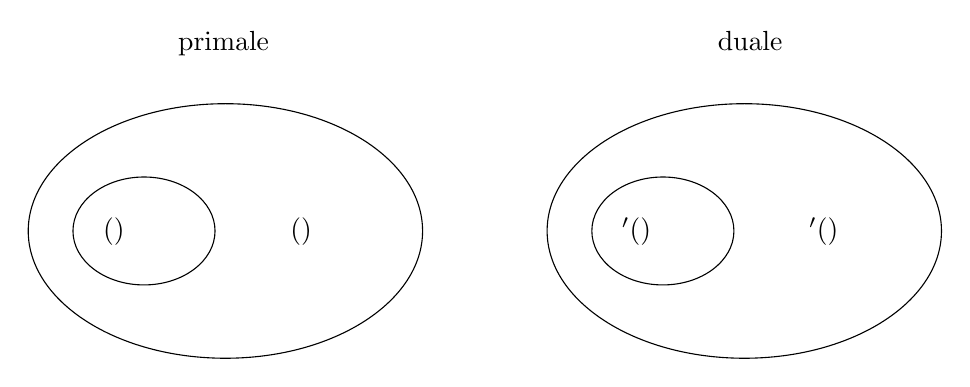
\begin{tikzpicture}[x = 0.75pt, y = 0.75pt, yscale = - 1, xscale = 1]
%uncomment if require: \path (0, 181); %set diagram left start at 0, and has height of 181

%Shape: Ellipse [id: dp7503563455876929]
\draw (80, 108.68) .. controls (80, 74.82) and (122.53, 47.36) .. (175, 47.36) .. controls (227.47, 47.36) and (270, 74.82) .. (270, 108.68) .. controls (270, 142.55) and (227.47, 170) .. (175, 170) .. controls (122.53, 170) and (80, 142.55) .. (80, 108.68) - - cycle;
%Shape: Ellipse [id: dp5108599722199094]
\draw (101.55, 108.68) .. controls (101.55, 94.32) and (116.87, 82.68) .. (135.77, 82.68) .. controls (154.68, 82.68) and (170, 94.32) .. (170, 108.68) .. controls (170, 123.04) and (154.68, 134.68) .. (135.77, 134.68) .. controls (116.87, 134.68) and (101.55, 123.04) .. (101.55, 108.68) - - cycle;
%Shape: Ellipse [id: dp5851131130928555]
\draw (330, 108.68) .. controls (330, 74.82) and (372.53, 47.36) .. (425, 47.36) .. controls (477.47, 47.36) and (520, 74.82) .. (520, 108.68) .. controls (520, 142.55) and (477.47, 170) .. (425, 170) .. controls (372.53, 170) and (330, 142.55) .. (330, 108.68) - - cycle;
%Shape: Ellipse [id: dp4435469561254657]
\draw (351.55, 108.68) .. controls (351.55, 94.32) and (366.87, 82.68) .. (385.77, 82.68) .. controls (404.68, 82.68) and (420, 94.32) .. (420, 108.68) .. controls (420, 123.04) and (404.68, 134.68) .. (385.77, 134.68) .. controls (366.87, 134.68) and (351.55, 123.04) .. (351.55, 108.68) - - cycle;

% Text Node
\draw (205, 101.08) node [anchor = north west][inner sep = 0.75pt] {$\Sc(\RR)$};
% Text Node
\draw (114.77, 101.08) node [anchor = north west][inner sep = 0.75pt] {$\Dc(\RR)$};
% Text Node
\draw (455, 101.08) node [anchor = north west][inner sep = 0.75pt] {$\Dc'(\RR)$};
% Text Node
\draw (364.77, 101.08) node [anchor = north west][inner sep = 0.75pt] {$\Sc'(\RR)$};
% Text Node
\draw (151, 11) node [anchor = north west][inner sep = 0.75pt] [align = left] {primale};
% Text Node
\draw (411, 11) node [anchor = north west][inner sep = 0.75pt] [align = left] {duale};

\end{tikzpicture}
\end{figure}
\FloatBarrier
Questa riduzione dello spazio, è una riduzione stretta, cioè perdiamo alcuni elementi, vediamo un esempio.
\begin{equation*}
u = e^{x^{2}} \in L^{1}_{\loc} \ \ \implies \ \ \text{c'è una distribuzione associata}
\end{equation*}
tuttavia se consideriamo come funzione test una funzione di $\Sc(\RR)$ $\varphi = e^{- x^{2}}$
\begin{equation*}
(u, \varphi) = \int_{\RR} u\varphi dx = \int_{\RR} dx = + \infty \ \ \implies \ \ \text{non è temperata}
\end{equation*}
\begin{defn}
[Convergenza di distribuzioni temperate]
Sia $u_{n}$ una successione in $\{u_{n}\} \subset \Sc'(\RR)$. Diciamo che $u_{n}\rightarrow u\in \Sc'(\RR)$ se per ogni funzione test a decrescita rapida $\varphi \in \Sc(\RR)$, si ha $(u_{n}, \varphi)\rightarrow (u, \varphi)$.
\end{defn}
La definizione di derivata è la stessa.

Ora chiediamoci, se consideriamo una funzione $u\in L^{1}_{\loc}$, possiamo dire che vi è associata una distribuzione temperata? Abbiamo questo risultato.
\begin{thm}
Se $\exists n\in \NN$ tale che $(1 + | x|)^{- n} u(x) \in L^{1}(\RR)$ allora esiste una distribuzione temperata associata $u\in \Sc'(\RR)$.
\end{thm}
\begin{thm}
Se $u\in L^{p}(\RR)$ per un qualsiasi $p\in [1, + \infty]$ allora esiste una distribuzione temperata associata $u\in \Sc'(\RR)$.
\end{thm}

\chapter{Trasformate integrali}

\section{Introduzione}

È la versione \textit{continua} della serie di Fourier. Vedremo tutto sulla retta reale, ma si può applicare anche in $\RR^{n}$. Consideriamo $\Dc(\RR) \subset L^{p}(\RR) \ \ \forall p\in [1, + \infty]$, questa inclusione è densa $\forall p < + \infty $ (escluso).
\begin{defn}
[Inclusione densa]
Dire che l'inclusione è densa significa dire che $\forall p < + \infty, \forall f\in L^{p}(\RR)$ esiste $\varphi_{n} \in \Dc(\RR)$ tale che $\varphi_{n}\rightarrow f$ in senso $L^{p}$, cioè $ \Vert \varphi_{n} - f \Vert_{L^{p}}\rightarrow 0$.
\end{defn}
Posso \textit{approssimare} ogni funzione in $L^{p}$ con $p < + \infty $ (funzioni anche molto irregolari e discontinue) con funzioni di $\Dc(\RR)$ (funzioni molto regolari e con cui è più semplice fare i conti), nel senso della norma ovviamente.

Introduciamo lo spazio
\begin{equation*}
\boxed{C^{0}_{0}(\RR) = \left\{f\in C^{0}(\RR), \lim_{x\rightarrow \pm \infty} f(x) = 0\right\}} \subset L^{\infty}(\RR)
\end{equation*}
Le funzioni in $C^{0}_{0}(\RR)$ sono automaticamente limitate, quindi contenute nello spazio $L^{\infty}(\RR)$ delle funzioni \textit{essenzialmente} limitate. Questa inclusione \textbf{non} è densa.

Sia $f\in L^{1}(\RR)$ definiamo la funzione traslata
\begin{equation*}
f_{y}(x) = f(x - y)
\end{equation*}
\begin{thm}
Sia $f\in L^{1}(\RR)$, allora
\begin{equation*}
\lim\limits_{y\rightarrow 0} \Vert f_{y} - f \Vert_{L^{1}} = 0
\end{equation*}
\end{thm}
\begin{proof}

È basata sulla densità a cui abbiamo accennato. Sia $\varepsilon > 0$, $\exists \varphi \in \Dc(\RR)$ tale che $ \Vert f - \varphi \Vert < \varepsilon $. Se trasliamo una funzione, essa non cambia di norma $\implies \ \Vert f_{y} - \varphi_{y} \Vert < \varepsilon $. Chiamiamo $K$ un certo insieme che contiene sia il supporto di $\varphi $ che della sua traslata $\varphi_{y}$, per un certo $y$ sufficientemente piccolo. Allora\footnote{Teorema di Heine - Cantor. Una funzione continua su un compatto è uniformemente continua.} la funzione $\varphi $ è uniformemente continua, cioè
\begin{gather*}
\forall \varepsilon > 0\ \ \exists \delta \ \ | \varphi (x) - \varphi (y)| < \varepsilon \ \ \text{purché} \ | x - y| < \delta \\
\Updownarrow \\
\forall \varepsilon > 0\ \ \exists \delta \ \ | \varphi (x - y) - \varphi (x)| < \varepsilon \ \ \text{purché} \ | y| < \delta
\end{gather*}
il delta che otteniamo \textit{non} dipende dal punto.

Dall'uniforme continuità deduciamo
\begin{equation*}
\Vert \varphi_{y} - \varphi \Vert = \int_{K}| \varphi (x - y) - \varphi (x)| dx < \varepsilon | K|
\end{equation*}
Veniamo ora a
\begin{align*}
\Vert f_{y} - f \Vert & = \Vert (f_{y} - \varphi_{y}) + (\varphi_{y} - \varphi) + (\varphi - f) \Vert \\
 & \leq \Vert f_{y} - \varphi_{y} \Vert + \Vert \varphi_{y} - \varphi \Vert + \Vert \varphi - f \Vert \\
 & < \varepsilon + \varepsilon | K| + \varepsilon \\
 & = \varepsilon (2 + | K|)
\end{align*}
dove $(2 + | K|)$ è costante e $\varepsilon $ è arbitrario, cioè $ \Vert f_{y} - f \Vert $ è tanto piccola quanto vogliamo.
\end{proof}

Prima di procedere riassumiamo brevemente le inclusioni fra gli spazi che abbiamo visto

\begin{center}

\begin{tabular}{lc}
$\Dc(\RR) \subset L^{p}(\RR)$ & densa $\forall p < + \infty $ \\
$\Dc(\RR) \subset L^{p}(\RR)$ & densa $\forall p < + \infty $ \\
$\Dc(\RR) \subset \Sc(\RR)$ & standard \\
$\Sc'(\RR) \subset \Dc'(\RR)$ & standard \\
$C^{0}_{0}(\RR) \subset L^{\infty}(\RR)$ & standard \\

\end{tabular}
\end{center}

\section{Trasformata di Fourier}

I numeri complessi entrano necessariamente nella trasformata di Fourier, quindi considereremo sempre funzioni $f: \RR\rightarrow \CC$.

Consideriamo $f\in L^{1}(\RR)$, definiamo \textbf{trasformata di Fourier} della funzione $f$
\begin{equation*}
\boxed{\hat{f}(z) = \int_{\RR} e^{- izx} f(x) dx} \ \ \ \ f\in L^{1}(\RR)
\end{equation*}
Ci ricordiamo che i coefficienti di Fourier erano
\begin{equation*}
c_{n} = \frac{1}{\pi}\int^{\pi}_{- \pi} e^{- inx} f(x) dx
\end{equation*}
È corretta la definizione?
\begin{equation*}
| f(x)| = \left| e^{- ixz} f(x)\right|
\end{equation*}
ma $f$, e quindi anche $| f| $, è integrabile secondo Lebesgue, quindi anche il secondo membro è integrabile e convergente. Ha senso dare questa definizione! Vediamo di capire le proprietà, riassunte nel teorema fondamentale.
\begin{thm}
[di Riemann - Lebesgue] Sia $f\in L^{1}(\RR)$, allora
\begin{equation*}
\boxed{\hat{f} \in C^{0}_{0}(\RR)} \ \ \ \ \boxed{\Vert \hat{f} \Vert_{\infty} \leq \Vert f \Vert_{L^{1}}}
\end{equation*}
\end{thm}
La trasformata ha proprietà molto diverse e molto più regolari della $f$, che è banalmente integrabile, sta in uno spazio compeltamente diverso.

\begin{proof}

\textit{Continuità.}

Sia $z_{n}\rightarrow z\in \RR$
\begin{equation*}
\lim\limits_{n\rightarrow + \infty}\hat{f}(z_{n}) = \lim\limits_{n\rightarrow + \infty}\int_{\RR} e^{- iz_{n} x} f(x) dx
\end{equation*}
Notiamo che abbiamo la convergenza puntuale, quasi $\forall x$. Se usassimo l'integrale di Riemann non avremmo questo risultato, con Lebesgue, sì, usando la convergenza dominata.
\begin{equation*}
g_{n}\rightarrow g\ \text{q.o.}, \ \exists h\in L^{1}, \ | g_{n}| \leq h\ \forall n\ \ \implies \ \ \lim\limits_{n\rightarrow + \infty}\int g_{n} = \int \lim\limits_{n\rightarrow + \infty} g_{n}
\end{equation*}
qui possiamo maggiorare
\begin{equation*}
\underbrace{\left| e^{- iz_{n} x} f(x)\right|}_{| g_{n}|} \leq \underbrace{| f(x)|}_{h} \in L^{1}
\end{equation*}
quindi
\begin{equation*}
\lim\limits_{n\rightarrow + \infty}\int_{\RR} e^{- iz_{n} x} f(x) dx = \int_{\RR}\lim\limits_{n\rightarrow + \infty} e^{- iz_{n} x} f(x) dx = \int_{\RR} e^{- izx} f(x) dx = \hat{f}(z)
\end{equation*}
\textit{Disuguaglianza delle norme.}

Chiaramente poi possiamo scrivere
\begin{equation*}
\Vert \hat{f} \Vert_{\infty} = | \hat{f}(z)| = \left| \int_{\RR} e^{- ixz} f(x) dx\right| \leq \int_{\RR}\left| e^{- ixz} f(x)\right| dx \leq \int_{\RR}| f(x)| dx = \Vert f \Vert_{L^{1}}
\end{equation*}
\textit{Ultima parte.}

Ci resta da far vedere che
\begin{equation*}
\lim\limits_{z\rightarrow \pm \infty}\hat{f}(z) = 0
\end{equation*}
Ricordiamo che $ - 1 = e^{i\pi}$, scriviamo
\begin{equation*}
\hat{f}(z) = - e^{i\pi}\int_{\RR} e^{- ixz} f(x) dx = - \int_{\RR} e^{- i(xz - \pi)} f(x) dx = - \int_{\RR} e^{- iz\left(x - \frac{\pi}{z}\right)} f(x) dx
\end{equation*}
cambiamo la variabile e ricordiamo che l'integrale è in $dx$
\begin{equation*}
x' = x - \frac{\pi}{z}
\end{equation*}
allora
\begin{equation*}
- \int_{\RR} e^{- iz\left(x - \frac{\pi}{z}\right)} f(x) dx = - \int_{\RR} e^{- izx'} f\left(x' + \frac{\pi}{z}\right) dx' = - \int_{\RR} e^{- izx} f\left(x + \frac{\pi}{z}\right) dx
\end{equation*}
Scriviamo ora il doppio di $\hat{f}$
\begin{align*}
2\hat{f}(z) & = \int_{\RR} e^{- ixz} f(x) dx - \int_{\RR} e^{- izx} f\left(x + \frac{\pi}{z}\right) dx\\
 & = \int_{\RR}\left[e^{- ixz} f(x) - e^{- izx} f\left(x + \frac{\pi}{z}\right)\right] dx\\
 & = \int_{\RR} e^{- ixz}\left[f(x) - f\left(x + \frac{\pi}{z}\right)\right] dx
\end{align*}
passiamo al modulo
\begin{align*}
2| \hat{f}(z)| & \leq \int_{\RR}\left| e^{- ixz}\left[f(x) - f\left(x + \frac{\pi}{z}\right)\right]\right| dx\\
 & = \int_{\RR}\left| f(x) - f\left(x + \frac{\pi}{z}\right)\right| dx\\
 & = \Vert f - f_{- \pi /z} \Vert_{L^{1}}
\end{align*}
Quando $z\rightarrow \pm \infty $ la traslazione $ - \pi /z\rightarrow 0$ e quindi, per quanto detto prima sulla traslazione di funzioni $L^{1}$ abbiamo $2| \hat{f}(z)| \rightarrow 0$.

\end{proof}

Questo vuol dire che se chiamiamo
\begin{equation*}
\Fc : L^{1}(\RR)\rightarrow C^{0}_{0}(\RR)
\end{equation*}
abbiamo un operatore trasformata di Fourier che è, ovviamente, lineare, e, grazie alla disuguaglianza $ \Vert \hat{f} \Vert_{\infty} \leq \Vert f \Vert_{L^{1}}$ anche limitata (e quindi equivalentemente anche continua, per quanto precedentemente). Cominciamo a verificare alcune proprietà.

Notazione: indichiamo con $\Fc(f(x), z) = \hat{f}(z)$ la trasformata di $f(x)$ scritta in funzione di $z$.
\begin{itemize}
\item Traslazione di $y\in \RR$.
\begin{align*}
\Fc(f(x - y), z) & = \int e^{- ixz} f(x - y) dx & x' = x - y\\
 & = \int e^{- ix'z - iyz} f(x') dx' & \\
 & = e^{- iyz}\int e^{- ixz} f(x) dx & \\
 & = e^{- iyz}\hat{f}(z) & \\
 & = e^{- iyz}\Fc(f(x), z) &
\end{align*}
\item Il contrario

\begin{align*}
\Fc\left(e^{iyx} f(x), z\right) & = \int e^{- ixz} e^{iyx} f(x) dx\\
 & = \int e^{- ix(z - y)} f(x) dx\\
 & = \hat{f}(z - y)\\
 & = \Fc(f(x), z - y)
\end{align*}
\item $\Fc\left(\overline{f(x)}, z\right) = \overline{\hat{f}(- z)}$
\item $f$ pari $\implies $ $\hat{f}$ pari
\item $f$ dispari $\implies $ $\hat{f}$ dispari
\item $f$ pari e reale $\implies $ $\hat{f}$ pari e reale
\item $f$ dispari e reale $\implies $ $\hat{f}$ dispari e immaginaria
\end{itemize}

Cerchiamo di capire se una trasformata di Fourier è derivabile, quindi anche $C^{1}$.
\begin{thm}
[Derivata della trasformata]
Sia $f\in L^{1}$, $g(x) = xf(x)$, $g\in L^{1}$. Allora $\hat{f} \in C^{1}$ e
\begin{equation*}
\hat{f}'(z) = - i\hat{g}(z) \ \ \text{cioè} \ \ \boxed{\frac{d^{n}}{dz^{n}}\Fc(f(x), z) = \Fc\left((- ix)^{n} \cdot f(x), z\right)}
\end{equation*}
\end{thm}
Chiedere che anche $xf(x)$ stia in $L^{1}$ significa che la $f$ deve in qualche senso tendere a $0$ abbastanza rapidamente, vogliamo che l'integrale su $\RR$ converga.

\begin{proof}

Calcoliamo il limite del rapporto incrementale
\begin{align*}
\lim\limits_{h\rightarrow 0}\frac{\hat{f}(z + h) - \hat{f}(z)}{h} & = \lim\limits_{h\rightarrow 0}\frac{1}{h}\left(\int e^{- ix(z + h)} f(x) dx - \int e^{- ixz} f(x) dx\right)\\
 & = \lim\limits_{h\rightarrow 0}\int e^{- ixz}\frac{e^{- ixh} - 1}{h} f(x) dx\\
 & = \int e^{- ixz}(- ix) f(x) dx\\
 & = - i\Fc(xf(x), z)\\
 & = - i\hat{g}(z)
\end{align*}
dove possiamo passare al limite sotto il segno di integrale perché in generale
\begin{equation*}
\left| e^{i\lambda} - 1\right| \leq | \lambda | \ \ \lambda \in \RR \ \ \ \ \ \ \ \ \lambda = - xh\ \ \implies \ \ \text{l'integrale converge per conv. dom.}
\end{equation*}
\end{proof}
\begin{thm}
[Trasformata della derivata]
Sia $f\in L^{1} \cap C^{1}$, $f'\in L^{1}$.
\begin{equation*}
\boxed{\Fc\left(\frac{d^{n}}{dx^{n}} f(x), z\right) = (iz)^{n} \cdot \Fc(f(x), z)}
\end{equation*}
\end{thm}
Tutto questo è vero purché le cose scritte abbiano senso, da cui le ipotesi.

\section{Trasformazione inversa}

\begin{thm}
Sia $f\in L^{1}$ e tale che $\hat{f} \in L^{1}$. Allora $f\in C^{0}_{0}$ e
\begin{equation*}
\boxed{f(x) = \frac{1}{2\pi}\int e^{ixz}\hat{f}(z) dz}
\end{equation*}
\end{thm}
Perché le richieste sugli spazi di appartenenza? Supponiamo che questa sia l'antitrasformata, ha senso? È corretta? C'è in generale questo problema
\begin{equation*}
\begin{array}{c c c}
f & \rightarrow & \hat{f}\\
\in L^{1} & & \in C^{0}_{0}
\end{array} \ \ \ \ \ \ \ \ \ \ \ \
\begin{array}{c c c}
\hat{f} & \rightarrow & f\\
\in L^{1} & & \in C^{0}_{0}
\end{array}
\end{equation*}
La trasformata di Fourier non è simmetrica, lavora su spazi diversi. Se vogliamo che sia simmetrica nel senso che mandi uno spazio nello stesso spazio e ci permetta di tornare indietro possiamo farlo prendendo uno spazio un po' strano: $L^{1} \cap C^{0}_{0}$, vale infatti (non dimostriamo)
\begin{equation*}
\Fc : L^{1} \cap C^{0}_{0}\rightarrow L^{1} \cap C^{0}_{0}
\end{equation*}
\textbf{Problema!} Lo spazio $L^{1} \cap C^{0}_{0}$ non è uno spazio di Banach, non è completo né rispetto alla norma $L^{1}$ né rispetto alla norma $L^{\infty}$. Cercheremo ora di estendere la definizione allo spazio $L^{2}$, che oltre a essere di Banach è anche di Hilbert
\begin{equation*}
\Fc : L^{2}\rightarrow L^{2}
\end{equation*}

\section{Convoluzione}

\begin{thm}
Siano $u, v\in L^{1}(\RR)$. Allora la funzione
\begin{equation*}
\boxed{(u*v)(x) = \int_{\RR} u(x - t) v(t) dt}
\end{equation*}
è definita per \underline{quasi ogni} $x\in \RR$, $(u*v) \in L^{1}$ e inoltre, stando in $L^{1}$, avrà una norma $ \Vert u*v \Vert_{L^{1}} \leq \Vert u \Vert_{L^{1}} \Vert v \Vert_{L^{1}}$.
\end{thm}
Discende direttamente dal teorema di Fubini.
\begin{itemize}
\item È simmetrica

\begin{align*}
(u*v)(x) & = \int_{\RR} u(x - t) v(t) dt & t' = x - t\\
 & = \int_{\RR} u(t') v(x - t') dt' & \\
 & = (v*u)(x) &
\end{align*}
\item È associativa
\begin{align*}
(u*v) *w & = u*(v*w)
\end{align*}
\item Supponiamo di avere

\begin{gather*}
u(x) =
\begin{cases}
n & x\in \left[0, \frac{1}{n}\right]\\
0 & \text{altrove}
\end{cases} \ \ \ \ \Vert u \Vert = 1\\
(u*v)(x) = \int_{\RR} u(x - t) v(t) dt = n\int^{x}_{x - \frac{1}{n}} v(t) dt
\end{gather*}

è la media della funzione $v$ calcolata in un intorno di $x$. L'effetto della convoluzione è in qualche modo di smussare il valore della funzione $v$, in ogni punto sostutiamo la media in un suo intorno.
\end{itemize}

Qual è il legame con la trasformata di Fourier? Siano $u, v\in L^{1}$, calcoliamo la trasformata di $u*v$, dato che sta in $L^{1}$
\begin{align*}
\Fc(u*v, z) & = \int e^{- ixz}\left[\int u(x - t) v(t) dt\right] dx\\
 & = \int e^{- iz(x - t)} e^{- izt} u(x - t) v(t) dtdx\\
 & = \int e^{- izt} v(t)\left[\int e^{- iz(x - t)} u(x - t) dx\right] dt
\end{align*}
con un cambio di variabile $x' = x - t$
\begin{align*}
\int e^{- izt} v(t)\left[\int e^{- iz(x - t)} u(x - t) dx\right] dt & = \int e^{- izt} v(t)\left[\int e^{- izx'} u(x') dx'\right] dt\\
 & = \hat{u}(z)\hat{v}(z)
\end{align*}
Vale anche il contrario
\begin{equation*}
\Fc^{- 1}(\hat{u} *\hat{v}, x) = u(x) v(x)
\end{equation*}

\section{Estensione della trasformata di Fourier}

Introduzione
\begin{itemize}
\item Ci serviremo della proprietà che $\Dc(\RR) \subset \Sc(\RR) \subset L^{p}(\RR)$ è un'inclusione densa per ogni $p < + \infty $
\item Lavoriamo in $\boxed{\Sc(\RR)}$ per estendere la trasformata perché la trasformata di una funzione in $\Sc(\RR)$ è ancora una funzione in $\Sc(\RR)$, mentre la trasformata di una funzione in $\Dc(\RR)$ è ancora $C^{\infty}$, ma non più necessariamente a supporto compatto.
\end{itemize}

\subsection{Allo spazio di funzioni a descrescenza rapida}

\begin{thm}
La trasformata agisce su
\begin{equation*}
\Fc : \Sc(\RR)\rightarrow \Sc(\RR)
\end{equation*}
\end{thm}
\begin{proof}

Lo spazio di partenza ha senso essendo densamente incluso in $L^{p}(\RR), p = 1$.

Sia $u\in S(\RR)$, consideriamo $v(x) = x^{N} u(x) \in \Sc(\RR) \subset L^{1}(\RR)$.
\begin{itemize}
\item Trasformata della derivata di $v$ $M$ volte
\begin{equation*}
\Fc\left(v^{(M)}, z\right) = (iz)^{M}\hat{v} \in L^{\infty}(\RR)
\end{equation*}

dato che $v$ sta in $L^{1}$, $\hat{v}$ sta in $C^{0}_{0}$, quindi la quantità $(iz)^{M}\hat{v}$ è limitata
\item Derivata della trasformata di $u$ $N$ volte
\begin{equation*}
\hat{u}^{(N)} = (- i)^{N}\hat{v}
\end{equation*}

moltiplichiamola per $z^{M}$, il termine che otteniamo a destra abbiamo appena fatto vedere che, a meno di coefficienti $i$ opportunamente elevati, è limitato
\begin{equation*}
z^{M}\hat{u}^{(N)} = z^{M}(- i)^{N}\hat{v} \ \ \boxed{\in L^{\infty}(\RR)} \ \ \forall N, M \geq 0
\end{equation*}ma questa è proprio la definizione di funzione a descrescenza rapida, quindi $\hat{u} \in \Sc(\RR)$ e abbiamo dimostrato la tesi.
\end{itemize}
\end{proof}

\subsection{Allo spazio $L^{2}$}

Vogliamo mostrare che
\begin{equation*}
\Fc : L^{2}(\RR)\rightarrow L^{2}(\RR)
\end{equation*}
Non possiamo definirla in $L^{2}$ come $\int e^{- ixz} u(x) dx$ perché se $u\in L^{2}$ non abbiamo nessuna garanzia che la funzione sia integrabile. Partiamo definendo la trasformata in $L^{1}(\RR) \cap L^{2}(\RR)$.
\begin{thm}
[di Plancherel]
Sia $u\in L^{1}(\RR) \cap L^{2}(\RR)$, allora
\begin{equation*}
\boxed{\Vert \hat{u} \Vert_{L^{2}} = \sqrt{2\pi} \Vert u \Vert_{L^{2}}} \ \ \text{quindi} \ \ \boxed{\hat{u} \in L^{2}(\RR)}
\end{equation*}
\end{thm}
\begin{proof}\leavevmode
\begin{itemize}
\item \textit{Dimostrazione nel caso di}$u\in \Sc(\RR)$

Dato che $u\in \Sc(\RR)$, allora $u\in L^{2}$. Ci serve partira da $u\in \Sc(\RR)$ per poter usare correttamente il risultato di inversione, in accordo a quanto appena detto sull'estensione a $\Fc : \Sc(\RR)\rightarrow \Sc(\RR)$.

\begin{align*}
\Vert u \Vert^{2}_{L^{2}} & = \int | u(x)|^{2} dx = \int \overline{u(x)} u(x) dx & \text{essendo} \ u\in L^{2}(\RR)\\
u(x) & = \frac{1}{2\pi}\int e^{ixz}\hat{u}(z) dz & \text{essendo} \ u\in \Sc(\RR)
\end{align*}

Sostituiamo

\begin{align*}
\Vert u \Vert^{2}_{L^{2}} & = \frac{1}{2\pi}\int \overline{u(x)}\int e^{ixz}\hat{u}(z) dzdx & \\
 & = \frac{1}{2\pi}\int \hat{u}(z)\int \overline{e^{- ixz} u(x)} dxdz & \text{(Fubini)}\\
 & = \frac{1}{2\pi}\int \hat{u}(z)\overline{\hat{u}(z)} dz & \\
 & = \frac{1}{2\pi} \Vert \hat{u} \Vert^{2}_{L^{2}} \ \ \implies \ \ \Vert \hat{u} \Vert_{L^{2}} = \sqrt{2\pi} \Vert u \Vert_{L^{2}} &
\end{align*}

Stando $u\in L^{2}$, ciò che sta a destra dell'uguale è un numero finito, quindi anche ciò che è a sinistra, quindi $\hat{u}$ appartiene ad $L^{2}$.
\item \textit{Estensione a}$u\in L^{2}(\RR)$

Per \textbf{densità} dell'inclusione $\Sc(\RR) \subset L^{2}(\RR)$,
\begin{itemize}
\item posso costruire una successione approssimante
\begin{equation*}
L^{2}(\RR) \supset \Sc(\RR) \ni u_{n}\xrightarrow{L^{2}} u\in L^{2}(\RR)
\end{equation*}
\item posso fare le trasformate $\widehat{u_{n}}$ dato che $u_{n} \in \Sc(\RR)$
\item per l'uguaglianza delle norme appena trovata, valida appunto per $u_{n} \in \Sc(\RR)$
\begin{equation*}
\Vert u_{n} - u_{m} \Vert_{L^{2}} = \Vert \hat{u}_{n} - \hat{u}_{m} \Vert_{L^{2}}\frac{1}{\sqrt{2\pi}}
\end{equation*}

Grazie alla completezza dello spazio $L^{2}$, se $u_{n}$ converge, è di Cauchy, allora lo è anche la sua trasformata, allora anche lei converge. Definisco $\hat{u}$ il limite della successione $\widehat{u_{n}}\xrightarrow{L^{2}}\hat{u}$, abbiamo trovato la trasformata $\Fc : L^{2}\rightarrow L^{2}$.
\end{itemize}
\item Con questo ragionamento potremmo anche dedurre che

\begin{equation*}
(u, v) = \frac{1}{2\pi}(\hat{u}, \hat{v}) \ \ \ \ \text{(si mantiene l'ortogonalità)}
\end{equation*}
\end{itemize}
\end{proof}

\section{Trasformata di Fourier di una distribuzione temperata}

Ci manca solo la trasformata di Fourier di una distribuzione temperata, consideriamo quindi $S'(\RR)$. Vogliamo mostrare che
\begin{equation*}
\Fc : S'(\RR)\rightarrow S'(\RR)
\end{equation*}
Ricordiamo che
\begin{equation*}
(u', \varphi) = - (u, \varphi')
\end{equation*}
Supponiamo che $u$ sia una distribuzione temperata $u\in \Sc'(\RR)$, vorremmo che $\hat{u} \in \Sc'(\RR)$. Definiamo senza nessuno sforzo
\begin{equation*}
\boxed{(\hat{u}, \varphi) = (u, \hat{\varphi})} \ \ \ \ \varphi \in \Sc(\RR)
\end{equation*}
dato che se $\varphi \in \Sc(\RR)$ allora $\hat{\varphi} \in \Sc(\RR)$.
\begin{thm}
La trasformata di Fourier $\Fc : \Sc'(\RR)\rightarrow \Sc'(\RR)$ è un'applicazione

lineare biunivoca e continua.
\end{thm}
\begin{proof}\leavevmode
\begin{itemize}
\item È effettivamente un funzionale \textbf{lineare} dalla definizione
\item \textbf{Continuo} grazie alla (non dimostrata) continuità della trasformata di Fourier delle funzioni in $\Sc(\RR)$.
\begin{equation*}
(\hat{u}, \varphi_{n}) = \left(u, \widehat{\varphi_{n}}\right)\rightarrow (u, \hat{\varphi}) = (\hat{u}, \varphi)
\end{equation*}
\item \textbf{Suriettiva.}
\begin{equation*}
\begin{array}{c c c}
\Fc : \Sc'(\RR) & \rightarrow & \Sc'(\RR)\\
u & & \hat{u} = v
\end{array}
\end{equation*}

Data una distribuzione temperata $v\in \Sc'(\RR)$ tale che $v = \hat{u}$ dobbiamo trovare $u\in \Sc'(\RR)$. Diciamo che $u = \Fc^{- 1}(v)$, e infatti
\begin{equation*}
(\hat{u}, \varphi) = (u, \hat{\varphi}) = \left(\Fc^{- 1}(v), \hat{\varphi}\right) = \left(v, \Fc^{- 1}(\hat{\varphi})\right) = (v, \varphi) \ \ \forall \varphi
\end{equation*}
\item \textbf{Iniettiva}.

Dobbiamo far vedere che se abbiamo $u_{1}, u_{2} \in \Sc'(\RR)$ e $\hat{u}_{1} = \hat{u}_{2}$ allora $u_{1} = u_{2}$. Prendiamo una nuova funzione test $\psi $ tale che $\hat{\psi} = \varphi $.
\begin{equation*}
(u_{1}, \varphi) = (u_{1}, \hat{\psi}) = (\hat{u}_{1}, \psi) = (\hat{u}_{2}, \psi) = (u_{2}, \hat{\psi}) = (u_{2}, \varphi)
\end{equation*}
\end{itemize}
\end{proof}
\textit{Esempio.}

Calcoliamo la trasformata di Fourier di una costante, cioè una funzione $L^{1}_{\loc}$ a cui quindi è associata una distribuzione temperata\footnote{Si noti che in testi differenti si potrebbe trovare un risultato diverso in base a come si è definita la trasformata di Fourier. Non tutti, infatti, sono d'accordo sull'uso della costante $2\pi $ tra la trasformazione diretta e quella inversa.}
\begin{equation*}
\Fc^{- 1}\{\delta_{0}(\xi)\} = \frac{1}{2\pi}\int_{\RR} e^{i\xi x} \delta_{0}(\xi) d\xi = \frac{1}{2\pi} \langle \delta_{0}(\xi), e^{i\xi x} \rangle = \frac{1}{2\pi}
\end{equation*}
allora
\begin{equation*}
\Fc\left\{\frac{1}{2\pi}\right\} = \delta_{0}(\xi) \ \ \implies \ \ \boxed{\Fc\{1\} = 2\pi \delta_{0}(\xi)}
\end{equation*}

\section{Trasformata di Laplace}

È parente stretta della trasformata di Fourier, solo che Fourier si riferisce a tutto $\RR^{n}$, Laplace su funzioni definite su una semiretta. Questa differenza si riflette sul loro impiego per le equazioni differenziali.

Cosa deve avere una funzione $u: \RR\rightarrow \RR$ affinché sia Laplace - trasformabile o $\Lc$ - trasformabile?
\begin{itemize}
\item $\supp(u) \subset [0, + \infty)$

A questo proposito ricordiamo la funzione di Heaviside, che sarà utile, in quanto non trasformeremo mai $\sin x$, piuttosto trasformeremo $H(x)\sin x$, anche se talvolta sorvoleremo su questa cosa dandola per scontata
\begin{equation*}
H(x) =
\begin{cases}
1, & \text{se} \ x \geq 0\\
0, & \text{se} \ x < 0
\end{cases}
\end{equation*}
\item $u\in L^{1}_{\loc}$
\item $\exists \lambda \in \RR$ tale che $e^{- \lambda x} u(x) \in L^{1}(\RR)$

Chiamiamo $\lambda (u)$ l'estremo inferiore di questi $\lambda $
\end{itemize}
\begin{defn}
[Trasformata di Laplace]
Definiamo
\begin{equation*}
\boxed{\Lc(u(x), s) = \int^{+ \infty}_{0} e^{- sx} u(x) dx} \ \ \ \ s\in \CC
\end{equation*}
dove
\begin{equation*}
e^{- sx} = e^{- s_{R} x} e^{- is_{I} x}
\end{equation*}
Questo integrale ha senso purché $e^{- \lambda x} u(x) \in L^{1}(\RR)$, cioè $\Re (s) > \lambda (u)$, che è quindi il dominio della trasformata, mentre Fourier aveva senso sempre.
\end{defn}
\textbf{Proprietà}
\begin{itemize}
\item Linearità $\boxed{\Lc(\alpha u(x) + \beta v(x), s) = \alpha \Lc(u(x), s) + \beta \Lc(v(x), s)}$

Attenzione, dobbiamo intersecare i due domini
\begin{equation*}
\boxed{\Re (s) > \max(\lambda (u), \lambda (v))}
\end{equation*}
\item $\boxed{\lim\limits_{\Re (s)\rightarrow + \infty}\Lc(u(x), s) = 0}$

\begin{proof}
\begin{equation*}
\lim\limits_{\Re (s)\rightarrow + \infty}\Lc(u(x), s) = \lim\limits_{\Re (s)\rightarrow + \infty}\int^{+ \infty}_{0} e^{- s_{R} x} e^{- is_{I} x} u(x) dx
\end{equation*}

possiamo portare il limite dentro per convergenza dominata, purché $\Re (s) > \lambda (u)$ possiamo trovare una funzione che la domini
\begin{equation*}
\lim\limits_{\Re (s)\rightarrow + \infty}\int^{+ \infty}_{0} e^{- s_{R} x} e^{- is_{I} x} u(x) dx = \int^{+ \infty}_{0}\lim\limits_{\Re (s)\rightarrow + \infty} e^{- s_{R} x} e^{- is_{I} x} u(x) dx = 0
\end{equation*}
\end{proof}
\item $\boxed{\Lc(u(x - x_{0}), s) = e^{- sx_{0}}\Lc(u(x), s)}$

Attenzione che essendo $\supp(u) \in [0, + \infty)$
\begin{itemize}
\item se $\boxed{x_{0} > 0}$ il supporto è ancora quello
\item se $x_{0} < 0$ il supporto potrebbe includere numeri negativi, quindi scartiamo questo caso
\end{itemize}

\begin{proof}
\begin{align*}
\Lc(u(x - x_{0}), s) & = \int^{+ \infty}_{0} e^{- sx} u(x - x_{0}) dx & x' = x - x_{0}\\
 & = \int^{+ \infty}_{- x_{0}} e^{- s(x' + x_{0})} u(x') dx' & \\
 & = \int^{+ \infty}_{0} e^{- s(x' + x_{0})} u(x') dx' & \\
 & = e^{- sx_{0}}\Lc(u(x), s) &
\end{align*}
\end{proof}
\item $\boxed{\Lc\left(e^{s_{0} x} u(x), s\right) = \Lc(u(x), s - s_{0})}$ $\boxed{\Re (s - s_{0}) > \lambda (u)}$

\begin{proof}
\begin{equation*}
\Lc\left(e^{s_{0} x} u(x), s\right) = \int^{+ \infty}_{0} e^{- x(s - s_{0})} u(x) dx = \Lc(u(x), s - s_{0})
\end{equation*}
\end{proof}
\item $\boxed{\Lc(u(cx), s) = \frac{1}{c}\Lc\left(u(x), \frac{s}{c}\right)}$ $\boxed{c\in \RR, c > 0}$

\begin{proof}
\begin{align*}
\Lc(u(cx), s) & = \int^{+ \infty}_{0} e^{- sx} u(cx) dx & x' = cx\ \ \implies \ \ dx' = cdx\\
 & = \int^{+ \infty}_{0} e^{- s\frac{x'}{c}} u(x')\frac{1}{c} dx' & \\
 & = \frac{1}{c}\Lc\left(u(x), \frac{s}{c}\right) &
\end{align*}
\end{proof}
\end{itemize}

\subsection{Trasformate di funzioni notevoli}

\begin{itemize}
\item Heaviside
\begin{align*}
\Lc(H(x), s) & = \int^{+ \infty}_{0} e^{- sx} H(x) dx = \int^{+ \infty}_{0} e^{- sx} dx\\
 & = \left[ - \frac{e^{- sx}}{s}\right]^{+ \infty}_{0} = \frac{1}{s} - \lim_{r\rightarrow + \infty}\frac{e^{- sr}}{s}\\
 & = \frac{1}{s} \ \ \ \ \text{purché} \ \Re (s) > 0
\end{align*}

il che ci dice anche che $\lambda (H) = 0$, confermato da
\begin{equation*}
e^{- \lambda x} H(x) \in L^{1}(\RR) \ \ \ \ \lambda > 0
\end{equation*}

Perché ci serve?
\begin{equation*}
\Lc\left(e^{s_{0} x} H(x), s\right) = \Lc(H(x), s - s_{0}) = \frac{1}{s - s_{0}}
\end{equation*}
\item Seno e coseno
\begin{align*}
\Lc(\cos(\omega x) H(x), s) & = \Lc\left(\frac{e^{i\omega x} + e^{- i\omega x}}{2}, s\right)\\
 & = \frac{1}{2}\left(\frac{1}{s - i\omega x} + \frac{1}{s + i\omega x}\right) = \frac{1}{2}\frac{2s}{s^{2} + \omega^{2}} = \frac{s}{s^{2} + \omega^{2}}\\
\Lc(\sin(\omega x) H(x), s) & = \frac{\omega}{s^{2} + \omega^{2}}
\end{align*}
\item Delta di Dirac \textit{trattandola come funzione}.
\begin{align*}
\Lc(\delta_{0}, s) & = \int^{+ \infty}_{0} e^{- sx} \delta_{0}(x) dx = 1
\end{align*}

per capirlo meglio possiamo vedere la Delta come
\begin{gather*}
\delta_{0} = \lim\limits_{\varepsilon \rightarrow 0} u_{\varepsilon}(x) \ \ \ \ u_{\varepsilon}(x) =
\begin{cases}
\frac{1}{\varepsilon}, & x\in [0, \varepsilon]\\
0, & \text{altrimenti}
\end{cases}\\
\Lc(u_{\varepsilon}(x), s) = \frac{1}{\varepsilon}\int^{\varepsilon}_{0} e^{- sx} dx = e^{- sx_{\varepsilon}}\rightarrow 1\ \ x_{\varepsilon} \in (0, \varepsilon)
\end{gather*}
\end{itemize}
\begin{thm}
[Derivata della trasformata]
Sia $u$ una funzione $\Lc$ - trasformabile.
\begin{equation*}
\boxed{\frac{d^{n}}{ds^{n}}\Lc(u(x), s) = (- 1)^{n} \Lc\left(x^{n} u(x), s\right)} \ \ \ \ \forall s\ \text{tale che} \ \Re (s) > \lambda (u)
\end{equation*}
\end{thm}
\begin{proof}
\begin{align*}
\lim\limits_{h\rightarrow 0}\frac{\Lc(u(x), s + h) - \Lc(u(x), s)}{h} & = \lim\limits_{h\rightarrow 0}\int^{+ \infty}_{0} e^{- sx}\frac{e^{- hx} - 1}{h} u(x) dx\\
 & = \int^{+ \infty}_{0}\lim\limits_{h\rightarrow 0} e^{- sx}\textcolor[rgb]{0.82, 0.01, 0.11}{\frac{e^{- hx} - 1}{- hx}}(- x) u(x) dx\\
 & = \int^{+ \infty}_{0} e^{- sx}(- x) u(x) dx\\
 & = - \Lc(xu(x), s)
\end{align*}
Possiamo passare al limite sotto il segno di integrale? Sì perché la quantità rossa è limitata, il resto è $L^{1}$.

È derivabile in un aperto in senso complesso, quindi la funzione trasformata di Laplace è olomorfa, quindi è anche $C^{\infty}$.
\begin{thm}
[Trasformata della derivata]
Sia $u$ una funzione $\Lc$ - trasformabile e $u\in C^{1}([0, + \infty))$. Chiamiamo $v(x)$ la derivata
\begin{equation*}
v(x) =
\begin{cases}
u'(x) & x \geq 0\\
0 & x < 0
\end{cases}
\end{equation*}
dove $u'(x)$ è estesa per continuità nell'origine.

Sia quindi anche $v$ $\Lc$ - trasformabile. Allora
\begin{equation*}
\boxed{\Lc(v(x), s) = s\Lc(u(x), s) - u(0)}
\end{equation*}
attenzione che in realtà $u(0)$ è il limite per $x\rightarrow 0^{+}$, dato che non è di solito continua nell'origine.

Inoltre
\begin{equation*}
\lim_{\Re (s)\rightarrow + \infty} s\Lc(u(x), s) = u(0)
\end{equation*}
Se $v\in L^{1}$, allora $\lambda (u) \leq 0$ e
\begin{equation*}
\lim\limits_{s\rightarrow 0, \ \Re (s) > 0} s\Lc(u(x), s) = \lim_{x\rightarrow + \infty} u(x)
\end{equation*}
\end{thm}
\textit{Dimostrazione della prima parte.}
\begin{align*}
\Lc(u'(x), s) & = \int^{+ \infty}_{0} e^{- sx} u'(x) dx & \text{(per parti)}\\
 & = \left[e^{- sx} u(x)\right]^{+ \infty}_{0} - (- s)\int^{+ \infty}_{0} e^{- sx} u(x) dx & \\
 & = \lim_{x\rightarrow + \infty} e^{- sx} u(x) - u(0) + s\Lc(u(x), s) &
\end{align*}
Notiamo che
\begin{equation*}
e^{- \lambda x} u(x) \in L^{1} \ \ \notimplies \ \ e^{- \lambda x} u(x)\rightarrow 0\ \text{per} \ x\rightarrow + \infty
\end{equation*}
per esempio questa funzione non tende a $0$ pur essendo integrabile



\begin{equation*}
\int^{+ \infty}_{0} f(x) dx = \sum^{\infty}_{n = 1}\frac{1}{n^{2}} < + \infty \ \ \ \ \text{ma} \ f(x) \nrightarrow 0
\end{equation*}
Analizziamo bene però la nostra funzione, derivandola
\begin{equation*}
\frac{d}{dx}\left(e^{- \lambda x} u(x)\right) = \underbrace{- \lambda e^{- \lambda x} u(x)}_{\in L^{1}} + \underbrace{e^{- \lambda x} u'(x)}_{\in L^{1}} \in L^{1}
\end{equation*}
le due parti sono integrabili per ipotesi, grazie al fatto che anche $u'$ deve essere $\Lc$ - trasformabile. Per il teoreoma del calcolo
\begin{equation*}
e^{- \lambda x} u(x) = u(0) + \int^{x}_{0}\frac{d}{dt}\left(e^{- \lambda t} u(t)\right) dt
\end{equation*}
il limite a destra esiste finito, allora esiste finito il limite di $e^{- \lambda x} u(x)$, ma se ammette limite deve necessariamente essere
\begin{gather*}
\lim_{x\rightarrow + \infty} e^{- sx} u(x) = 0
\end{gather*}
\end{proof}

\subsection{Trasformazione inversa}

Se abbiamo $f(s) = \Lc(u(x), s)$ come troviamo $u(x) = \Lc^{- 1}(f(s), s)$?

Scriviamo $s = a + ib$.
\begin{equation*}
f(a + ib) = \int^{+ \infty}_{0} e^{- ax} e^{- ibx} u(x) dx = \int_{\RR} e^{- ax} e^{- ibx} u(x) dx = \Fc\left(e^{- ax} u(x), b\right)
\end{equation*}
Ma allora possiamo fare l'antitrasformata di Fourier!
\begin{equation*}
e^{- ax} u(x) = \frac{1}{2\pi}\int_{\RR} f(a + ib) e^{ibx} db
\end{equation*}
allora
\begin{equation*}
\boxed{u(x) = \frac{1}{2\pi}\int_{\RR} e^{(a + ib) x} f(a + ib) db} \ \ \ \ \forall a > \lambda (u)
\end{equation*}
Questa è già una formula valida, ma possiamo chiamare, per $x$ fissato
\begin{equation*}
\Gamma_{x} = \{z\in \CC, z = x + iy, y\in \RR\}
\end{equation*}

\begin{figure}[htpb]
\centering
\tikzset{every picture/.style = {line width = 0.75pt}} %set default line width to 0.75pt

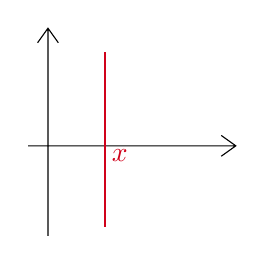
\begin{tikzpicture}[x = 0.75pt, y = 0.75pt, yscale = - 1, xscale = 1]
%uncomment if require: \path (0, 113); %set diagram left start at 0, and has height of 113

%Shape: Axis 2D [id: dp6665420354493967]
\draw (251, 63.66) - - (351, 63.66)(260.5, 7) - - (260.5, 107) (344, 58.66) - - (351, 63.66) - - (344, 68.66) (255.5, 14) - - (260.5, 7) - - (265.5, 14);
%Straight Lines [id: da4009061220418899]
\draw [color = {rgb, 255: red, 208; green, 2; blue, 27}, draw opacity = 1] (288, 18.66) - - (288, 103);

% Text Node
\draw (290, 64.23) node [anchor = north west][inner sep = 0.75pt] [color = {rgb, 255: red, 208; green, 2; blue, 27}, opacity = 1] {$x$};

\end{tikzpicture}
\end{figure}
\FloatBarrier

E possiamo allora scrivere l'antitrasformata come
\begin{equation*}
\boxed{u(x) = \frac{1}{2\pi}\int_{\Gamma_{x}} e^{zx} f(z) dz}
\end{equation*}

\section{Relazione con la convoluzione}

Ricordiamo la convoluzione di due funzioni $f, g\in L^{1}$
\begin{equation*}
(f*g)(x) = \int_{\RR} f(x - t) g(t) dt
\end{equation*}
Con Fourier abbiamo, utile in entrambi i versi,
\begin{equation*}
\Fc(f*g, z) = \hat{f}(z)\hat{g}(z)
\end{equation*}
Per Laplace abbiamo le seguenti richieste sulle funzioni affinché siano $\Lc$ - trasformabili
\begin{itemize}
\item $f, g\in L^{1}_{\loc}$
\item $\supp f\subset [0, + \infty), \ \supp g\subset [0, + \infty)$
\item $\exists \lambda_{1}, \lambda_{2} \ \implies \ e^{- \lambda_{1} x} f(x) \in L^{1}(\RR), \ e^{- \lambda_{2} x} g(x) \in L^{1}(\RR)$
\end{itemize}
\begin{thm}
La convoluzione di due funzioni trasformabili secondo Laplace, è trasformabile secondo Laplace.
\end{thm}
\begin{proof}
\begin{equation*}
(f*g)(x) = \int_{\RR} f(x - t) g(t) dt = \int^{x}_{0} f(x - t) g(t) dt
\end{equation*}
$f(x - t) = 0$ se $x - t < 0$, quindi se $t > x$. Mentre $g(t) = 0$ se $t < 0$. Allora esiste l'integrale.
\begin{align*}
e^{- \lambda x}(f*g)(x) & = e^{- \lambda x}\int^{x}_{0} f(x - t) g(t) dt\\
 & = \int^{x}_{0} e^{- \lambda (x - t)} f(x - t) e^{- \lambda t} g(t) dt\\
 & = \left(e^{- \lambda x} f(x)\right) *\left(e^{- \lambda x} g(x)\right) \ \ \ \ \lambda \geq \max(\lambda (f), \lambda (g)) \ \implies \ \in L^{1}
\end{align*}
Soddisfa i requisiti, calcoliamone l'espressione
\begin{align*}
\Lc((f*g), s) & = \int_{\RR} e^{- sx}\left(\int_{\RR} f(x - t) g(t) dt\right) dx\\
 & = \iint_{\RR^{2}} e^{- s(x - t)} e^{- st} f(x - t) g(t) dtdx\\
 & = \int_{\RR} e^{- s(x - t)} f(x - t)\int_{\RR} e^{- st} g(t) dtdx = (\star)
\end{align*}
cambiamo la variabile $x' = x - t$
\begin{gather*}
(\star) = \left[\int_{\RR} e^{- sx'} f(x') dx'\right]\left[\int_{\RR} e^{- st} g(t) dt\right] = \Lc(f) \cdot \Lc(g)
\end{gather*}
\end{proof}

\chapter{Conclusioni}

\section{EDP e Fourier}

Consideriamo l'equazione del calore
\begin{equation*}
u_{t} - u_{xx} = 0\ \ \ \ u(t, x) \ \ \ \ u_{t} = \partial_{t} u\ \ \ \ u_{xx} = \partial_{x} \partial_{x} u\ \ \ \ x\in \RR, t \geq 0
\end{equation*}
Supponiamo di sapere il dato iniziale
\begin{equation*}
\begin{cases}
u_{t} - u_{xx} = 0\\
u(0, x) = g(x)
\end{cases}
\end{equation*}
Indico con
\begin{equation*}
\hat{u}(t, z) = \int_{\RR} e^{izx} u(t, x) dx
\end{equation*}
trattando $t$ come un parametro
\begin{align*}
\frac{\partial}{\partial t}\hat{u}(t, z) & = \frac{\partial}{\partial t}\int_{\RR} e^{izx} u(t, x) dx\overset{!!!}{=}\int_{\RR} e^{izx}\frac{\partial}{\partial t} u(t, x) dx = \Fc(u_{t}(t, x), z)\\
 & \\
\Fc(u_{xx}(t, x), z) & = \int_{\RR} e^{- ixz} u_{xx}(t, x) dx\ \ \forall t \geq 0\\
 & \overset{\text{ipp}}{=}\int_{\RR}(iz)^{2} e^{- ixz} u(t, x) dx\\
 & = - z^{2}\Fc(u(t, x), z)
\end{align*}
Allora il problema diventa
\begin{equation*}
\begin{cases}
\partial_{t}\hat{u}(t, z) + z^{2}\hat{u}(t, z) = 0\\
\hat{u}(0, z) = \hat{g}(z)
\end{cases}
\end{equation*}
per ogni $z$, è un'equazione differenziale ordinaria
\begin{equation*}
\hat{u}(t, z) = \hat{g}(z) e^{- z^{2} t}
\end{equation*}
antitrasformiamo
\begin{equation*}
u(t, x) = \Fc^{- 1}\left(\hat{g}(z) e^{- z^{2} t}, x\right)
\end{equation*}
torna utile il prodotto di convoluzione
\begin{gather*}
u(t, x) = g(x) *\Fc^{- 1}\left(e^{- z^{2} t}, x\right) = \frac{1}{\sqrt{4\pi t}}\int_{\RR} e^{- \frac{(x - y)^{2}}{2t}} g(y) dy\\
\Fc^{- 1}\left(e^{- z^{2} t}, x\right) = \frac{1}{\sqrt{4\pi t}} e^{- \frac{x^{2}}{2t}}
\end{gather*}
ma non è definita in $t = 0$, tuttavia possiamo considerare il limite nel senso delle distribuzioni (non dimostrato, molto extra)
\begin{equation*}
\lim_{t\rightarrow 0^{+}} u(t, x) = g(x) \ \ \ \ u(t, x) : [0, + \infty) \times \RR \ \ \ \ g: \RR\rightarrow \RR
\end{equation*}

\section{EDP e Laplace}

Con Laplace risolviamo cose del tipo
\begin{equation*}
\begin{cases}
a_{n} y^{(n)}(t) + a_{n - 1} y^{(n - 1)}(t) + \cdots + a_{0} y(t) = f(t)\\
y^{(n - 1)}(0) = \textcolor[rgb]{0.82, 0.01, 0.11}{y}\textcolor[rgb]{0.82, 0.01, 0.11}{_{n - 1}}\\
\vdots \\
y(0) = \textcolor[rgb]{0.29, 0.56, 0.89}{y}\textcolor[rgb]{0.29, 0.56, 0.89}{_{0}}
\end{cases}
\end{equation*}
Trasformiamo
\begin{align*}
\Lc(y'(t), s) & = s\Lc(y(t), s) - y(0)\\
\Lc(y''(t), s) & = s\Lc(y'(t), s) - y'(0)\\
 & = s[s\Lc(y(t), s) - y(0)] - y'(0)\\
 & = s^{2}\Lc(y(t), s) - sy(0) - y'(0)\\
\Lc\left(y^{(n)}(t), s\right) & = s^{n}\Lc(y(t), s) - s^{n - 1}\textcolor[rgb]{0.29, 0.56, 0.89}{y}\textcolor[rgb]{0.29, 0.56, 0.89}{(}\textcolor[rgb]{0.29, 0.56, 0.89}{0}\textcolor[rgb]{0.29, 0.56, 0.89}{)} - s^{n - 1} y'(0) - \cdots - \textcolor[rgb]{0.82, 0.01, 0.11}{y}\textcolor[rgb]{0.82, 0.01, 0.11}{^{(n - 1)}}\textcolor[rgb]{0.82, 0.01, 0.11}{(}\textcolor[rgb]{0.82, 0.01, 0.11}{0}\textcolor[rgb]{0.82, 0.01, 0.11}{)}
\end{align*}
Esempio del secondo ordine
\begin{equation*}
\begin{cases}
a_{2} y''(y) + a_{1} y'(t) + a_{0} y(t) = f(t)\\
y(0) = y_{0}\\
y'(0) = y_{1}
\end{cases}
\end{equation*}
Trasformiamo
\begin{align*}
a_{2}\left(s^{2}\Lc(y(t), s) - sy_{0} - y_{1}\right) + a_{1}(s\Lc(y(t), s) - y_{0}) + a_{0}\Lc(y(t), s) & = \Lc(f(t), s)\\
\left(a_{2} s^{2} + a_{1} s + a_{0}\right)\Lc(y(t), s)\underbrace{- a_{2}(sy_{0} + y_{1}) - a_{1} y_{0}}_{\text{polinomio in} \ s} & = \Lc(f(t), s)
\end{align*}
quindi
\begin{equation*}
	\Lc(y(t), s) = \frac{\Lc(f(t), s) + a_{2}(sy_{0} + y_{1}) + a_{1} y_{0}}{a_{2} s^{2} + a_{1} s + a_{0}}
\end{equation*}
ci permette di introdurre in maniera naturale anche i dati iniziali.
\begin{gather*}
y(t) = f(t) *\Lc^{- 1}\left(\frac{1}{a_{2} s^{2} + a_{1} s + a_{0}}, t\right) + \Lc^{- 1}\left(\frac{a_{2}(sy_{0} + y_{1}) + a_{1} y_{0}}{a_{2} s^{2} + a_{1} s + a_{0}}, t\right)\\
\\
\frac{1}{s - s_{0}} + \frac{1}{s - s_{1}} + \cdots \ \ \ \ \Lc\left(e^{\alpha t} H(t), s\right) = \frac{1}{s - \alpha}
\end{gather*}

\section{Trasformata vs Serie di Fourier}

Sono definite da
\begin{equation*}
\hat{f}(z) = \int_{\RR} e^{- ixz} f(x) dx\ \ \ \ \ \ \ \ f(x) = \sum_{n\in \ZZ} e^{inx} c_{n}
\end{equation*}
Agiscono sugli spazi
\begin{equation*}
\Fc : L^{2}(A)\rightarrow L^{2}(A) \ \ \ \ \ \ \ \ L^{2}[ - \pi, \pi]\rightarrow l^{2}
\end{equation*}
Valgono due identità importanti
\begin{equation*}
\Vert f \Vert_{L^{2}} = \frac{1}{\sqrt{2\pi}} \Vert \hat{f} \Vert_{L^{2}} \ \ \text{(Plancherel)} \ \ \ \ \ \ \ \ \Vert f \Vert_{L^{2}} = \sqrt{\pi} \Vert c \Vert_{l^{2}} \ \ \text{(Parseval)}
\end{equation*}
dove
\begin{equation*}
\{c_{n}\} \in l^{2}, \ \text{ovvero} \ \ \sum\nolimits_{n\in \ZZ}| c_{n}|^{2} < + \infty
\end{equation*}
Infine se per la serie prendiamo come dominio $L^{2}([ - L, L])$ e facciamo tendere $L\rightarrow \infty $, la serie
\begin{equation*}
f(x) = \sum_{n\in \ZZ} e^{i\frac{2\pi}{L} nx} c_{n}
\end{equation*}
viene fatta su una griglia sempre più fine e inizia ad assomigliare all'integrale!



\part{Esercizi}
%           TEMPLATE

%           \chapter{Spazi campionari}
%           
%           \ParteEsercizi
%           
%           \Esercizio{(Nome di un esercizio speciale)}
%           \Esercizio{}
%           \Esercizio{}
%           
%           \ParteSoluzioni
%           
%           \Soluzione
%           \Soluzione
%           \Soluzione
%           
%           
%           \chapter{Indipendenza}
%           
%           \ParteEsercizi
%           
%           \Esercizio{}
%           \begin{enumerate}
%               \item ine
%               \item oh
%               \item $\!\!\!\!{^*}$ jhk b
%           \end{enumerate}
%           \Esercizio{$*$}
%           \Esercizio{}
%           
%           \ParteSoluzioni
%           
%           \Soluzione
%           \Soluzione
%           \Soluzione









\chapter{Esercitazione 1 - Boella}
\ParteEsercizi
\Esercizio{}

Risolvere l'equazione
\begin{equation*}
\sin z=2
\end{equation*}
\Esercizio{}

Scrivere la serie di potenze di
\begin{equation*}
f(z)=\frac{1}{z^{2} -3z+2}
\end{equation*}
\Esercizio{}

Scrivere la serie di potenze di
\begin{equation*}
f(z)=\frac{e^{z}}{1+2z}
\end{equation*}
\Esercizio{}

La funzione
\begin{equation*}
u(x,y)=y^{3} -3x^{2} y
\end{equation*}
è armonica? Qual è la sua armonica coniugata?
\Esercizio{}

Calcolare $\int\nolimits _{\gamma _{1}} f(z)dz$ con
\begin{equation*}
f(z)=\overline{z} \ \ \ \ \gamma _{1} =\left( t,it^{2}\right) \ \ \ \ t\in [0,1]
\end{equation*}
\Esercizio{}

Calcolare $\int\nolimits _{\gamma _{1}} f(z)dz$ con
\begin{equation*}
f(z)=\overline{z} \ \ \ \ \gamma _{2} =(t,it)\ \ \ \ 
\end{equation*}
\Esercizio{}

Calcolare $\int _{\gamma _{1}} g(z)dz$ e $\int _{\gamma _{2}} g(z)dz$ con
\begin{equation*}
g(z)=z^{2} \ \ \ \ \gamma _{1} =\left( t,it^{2}\right) \ \ \ \ \gamma _{2} =(t,it)\ \ \ \ t\in [0,1]
\end{equation*}
\ParteSoluzioni
\Soluzione
\begin{theorem}
[Formule di Eulero] Il seno e il coseno complessi possono essere espressi come
\begin{equation*}
\sin z=\frac{e^{iz} -e^{-iz}}{2i} \ \ \cos z=\frac{e^{iz} +e^{-iz}}{2}
\end{equation*}
\end{theorem}
Si ha
\begin{align*}
\sin z=\frac{e^{iz} -e^{-iz}}{2i} & =2\\
e^{iz} -4i-e^{-iz} & =0\\
e^{2iz} -4ie^{iz} -1 & =0
\end{align*}
ponendo $w=e^{iz}$ abbiamo
\begin{equation*}
w^{2} -4iw-1=0\ \ \Rightarrow \ \ w=2i\pm \sqrt{3} i=(2\pm \sqrt{3} )i
\end{equation*}
Eguagliamo quindi
\begin{equation*}
(2\pm \sqrt{3} )i=e^{iz}
\end{equation*}
Ricordiamo che $z=x+iy$ e da ciò segue che
\begin{equation*}
e^{iz} =e^{ix-y} =e^{-y} e^{ix} \ \ \ \ \ \ \ \ (2\pm \sqrt{3} )i=(2\pm \sqrt{3} )e^{i\pi /2}
\end{equation*}
Uguagliando il modulo abbiamo
\begin{equation*}
e^{-y} =(2\pm \sqrt{3} )\ \ \Rightarrow \ \ y=-\ln (2\pm \sqrt{3} )
\end{equation*}
Uguagliando l'argomento abbiamo
\begin{equation*}
e^{ix} =e^{i\pi /2} \ \ \Rightarrow \ \ x=\frac{\pi }{2} +2k\pi 
\end{equation*}
L'equazione ha quindi \textit{infinite} soluzioni, date da infinite coppie di punti disposti su due rette parallele.
\Soluzione
\begin{definition}
La serie centra nel punto $z_{0}$ è data da
\begin{equation*}
\sum\limits ^{\infty }_{n=0} a_{n}\left( z-z_{0}\right)^{n}
\end{equation*}
\end{definition}
\begin{nb}
Il raggio di convergenza è $R$, ed è centrato in $z_{0}$. In tutti i punti interni la serie converge, nei punti esterni non converge, sulla circonferenza nulla si può dire in generale.
\end{nb}
\begin{theorem}
[Criterio del rapporto]
\begin{equation*}
\frac{1}{R} =\lim\limits _{n\rightarrow +\infty }\frac{\left| a_{n+1}\right| }{\left| a_{n}\right| }
\end{equation*}
Se il limite vale $\infty /0$, il raggio è $0/\infty $. Se il limite non esiste, il criterio fallisce.
\end{theorem}
\begin{theorem}
[Criterio della radice]
\begin{equation*}
\frac{1}{R} =\limsup\limits _{n\rightarrow \infty }\sqrt[n]{\left| a_{n}\right| }
\end{equation*}
Si noti che il limite superiore esiste sempre (a differenza del limite).
\end{theorem}
\begin{definition}
Serie prodotto secondo Cauchy
\begin{equation*}
A=\sum\limits ^{\infty }_{n=0} a_{n} ,\ \ B=\sum\limits ^{\infty }_{n=0} b_{n} \ \ \Rightarrow \ \ C=\sum\limits ^{\infty }_{n=0} a_{n}\sum\limits ^{\infty }_{n=0} b_{n} =\sum\limits ^{\infty }_{n=0} c_{n}
\end{equation*}
con
\begin{equation*}
c_{n} =\sum\limits ^{n}_{k=0} a_{k} b_{n-k}
\end{equation*}
\end{definition}
\begin{theorem}
La serie $C$ converge assolutamente ad $A\cdot B$, per il teorema di Mertens, se almeno una fra $A$ e $B$ converge assolutamente.

Se $A$ e $B$ hanno $R=+\infty ,$ si può ovviamente applicare il teorema di Mertens, e si può scrivere
\begin{equation*}
\sum\limits ^{\infty }_{n=0} a_{n}\sum\limits ^{\infty }_{n=0} b_{n} =\sum\limits ^{\infty }_{n,m=0} a_{n} b_{m}
\end{equation*}
\end{theorem}
\begin{nb}
[Serie notevoli]
\begin{align*}
e^{z} & =\sum ^{\infty }_{n=0}\frac{z^{n}}{n!} & R=+\infty \\
\cosh z & =\sum ^{\infty }_{n=0}\frac{z^{2n}}{(2n)!} & R=+\infty \\
\sinh z & =\sum ^{\infty }_{n=0}\frac{z^{2n+1}}{(2n+1)!} & R=+\infty \\
\cos z & =\sum ^{\infty }_{n=0}\frac{(-1)^{n} z^{2n}}{(2n)!} & R=+\infty \\
\sin z & =\sum ^{\infty }_{n=0}\frac{(-1)^{n} z^{2n+1}}{(2n+1)!} & R=+\infty \\
\frac{1}{1-z} & =\sum ^{\infty }_{n=0} z^{n} & R=1
\end{align*}
\end{nb}
Separiamo in due termini la frazione
\begin{equation*}
f(z)=\frac{1}{z^{2} -3z+2} =\frac{1}{( z-1)( z-2)} =\frac{1}{z-2} -\frac{1}{z-1} =\frac{1}{1-z} -\frac{1}{2-z}
\end{equation*}
Raccogliamo nel secondo termine
\begin{equation*}
\frac{1}{2-z} =\frac{\frac{1}{2}}{1-\frac{z}{2}} =\frac{1}{2}\frac{1}{1-\frac{z}{2}}
\end{equation*}
valgono poi
\begin{equation*}
\frac{1}{1-z} =\sum ^{\infty }_{n=0} z^{n} \ \ \ \ \frac{1}{2-z} =\frac{1}{2}\sum ^{\infty }_{n=0}\left(\frac{z}{2}\right)^{n} =\sum ^{\infty }_{n=0}\frac{1}{2^{n+1}} z^{n}
\end{equation*}
pertanto
\begin{equation*}
f(z)=\sum ^{\infty }_{n=0}\left( 1-\frac{1}{2^{n+1}}\right) z^{n}
\end{equation*}
Il raggio di convergenza è l'intersezione tra $|z|< 1$ e $|z|< 2$, ovvero $|z|< 1$.
\Soluzione
\begin{equation*}
f(z)=\frac{e^{z}}{1+2z} =e^{z} \cdotp \frac{1}{1-( -2z)} =( *)
\end{equation*}
Sviluppiamo in serie e scriviamo la serie prodotto secondo Cauchy
\begin{equation*}
( *) =\sum ^{\infty }_{n=0}\frac{z^{n}}{n!} \cdotp \sum ^{\infty }_{m=0} (-2z)^{m} =\sum ^{\infty }_{n=0}\sum ^{n}_{k=0}\frac{z^{k}}{k!} (-2)^{n-k} z^{n-k} =\sum ^{\infty }_{n=0}\left(\sum ^{n}_{k=0}\frac{(-2)^{n-k}}{k!}\right) z^{n}
\end{equation*}
In alternativa, sfruttando Mertens
\begin{equation*}
f(z)=\frac{e^{z}}{1+2z} =\sum ^{\infty }_{n=0}\frac{z^{n}}{n!} \cdotp \sum ^{\infty }_{n=0} (-2z)^{n} =\sum ^{\infty }_{n,m=0}\frac{z^{n}}{n!} (-2)^{m} z^{m}
\end{equation*}
\Soluzione
\begin{definition}
Una funzione si dice \textbf{armonica} se la somma delle sue derivate seconda è pari a zero.
\end{definition}
\begin{definition}
Una funzione si dice \textbf{olomorfa} se è derivabile in senso complesso.
\end{definition}
\begin{theorem}
Sia $f(z)$ olomorfa: $f(z)=f(x,y)=u(x,y)+iv(x,y)$. Allora $u$ e $v$ sono armoniche, e l'una è l'armonica coniugata dell'altra, secondo le condizioni di Cauchy-Riemann
\begin{equation*}
u_{x} =v_{y} \ \ \ \ u_{y} =-v_{x}
\end{equation*}
\end{theorem}
Deriviamo la funzione
\begin{gather*}
u_{x} =-6xy=v_{y}\\
u_{y} =3y^{2} -3x^{2} =-v_{x}
\end{gather*}
pertanto è armonica.

Integrando la $v_{x}$ abbiamo
\begin{equation*}
\int v_{x} dx=\int \left( 3x^{2} -3y^{2}\right) dx=x^{3} -3xy^{2} +h(y)
\end{equation*}
integrando la $v_{y}$ abbiamo
\begin{equation*}
\int v_{y} dy=\int -6xydy=-3xy^{2} +k(x)
\end{equation*}
Da ciò segue che $k(x)=x^{3}$ e $h(y)=\text{costante}$. Pertanto
\begin{equation*}
v(x,y)=x^{3} -3xy^{2}
\end{equation*}
e
\begin{align*}
f(z) & =f(x,y)\\
 & =u(x,y)+iv(x,y)\\
 & =\left( y^{3} -3x^{2} y\right) +i\left( x^{3} -3xy^{2}\right)\\
 & =iz^{3}
\end{align*}
\Soluzione

È noto che
\begin{equation*}
f(z)=\overline{z} =x-iy\ \ \ \ dz=d\left( t+it^{2}\right) =dt+2itdt=\left( 1+2it\right) dt
\end{equation*}
Pertanto
\begin{align*}
\int _{\gamma _{1}} f(z)dz & =\int ^{1}_{0}\left( t-it^{2}\right) (1+2it)dt\\
 & =\int ^{1}_{0}\left( t+it^{2} +2t^{3}\right) dt\\
 & =\left[\frac{t^{2}}{2} +i\frac{t^{3}}{3} +\frac{t^{4}}{2}\right]^{1}_{0}\\
 & =1+\frac{i}{3}
\end{align*}
\Soluzione

È noto che
\begin{gather*}
f(z)=\overline{z} =x-iy\\
dz=dx+idy\\
dx=dt\\
dy=dt
\end{gather*}
Pertanto
\begin{equation*}
\int _{\gamma _{2}} f(z)dz=\int ^{1}_{0} (t-it)(1+i)dt=\int ^{1}_{0} 2tdt=1
\end{equation*}
Notiamo che l'integrale dipende dal percorso scelto, essendo $\overline{z}$ una funzione \textit{non} olomorfa.
\Soluzione

Osserviamo che
\begin{gather*}
z^{2} =x^{2} -y^{2} +2ixy\\
dx+idy=dt+2itdt
\end{gather*}
Pertanto
\begin{align*}
\int _{\gamma _{1}} g(z)dz & =\int ^{1}_{0}\left( t^{2} -t^{4} +2it^{3}\right) (1+2it)dt\\
 & =\left[\frac{t^{3}}{3} +it^{4} -5t^{5} -\frac{i}{3} t^{6}\right]^{1}_{0}\\
 & =-\frac{2}{3} +\frac{2}{3} i
\end{align*}
\textit{Esercizio:} svolgere l'integrale $\gamma _{2}$, spiegando perché ora il risultato sia uguale.
\chapter{Esercitazione 1 - Potrich}
\ParteEsercizi
\Esercizio{}

Determinare in quali punti del piano complesso la funzione
\begin{equation*}
f\left( z\right) =z^{2}\left| z\right| ^{2} e^{i\overline{z}^{2}}
\end{equation*}
è derivabile in senso complesso.
\Esercizio{}

Mostrare che
\begin{equation*}
u\left( x,y\right) =2x-2xy
\end{equation*}
è armonica e trovare la sua armonica coniugata.
\Esercizio{}

Sia $\gamma \left( t\right) =t+it^{2} ,t\in \left[ -1,0\right]$. Calcolare
\begin{equation*}
\int\nolimits _{\gamma }\left[\overline{z} +\left( z+1\right)^{7}\right] dz
\end{equation*}
\Esercizio{}

Calcolare
\begin{equation*}
\int\nolimits _{\gamma }\left(\overline{z}\right)^{2} dz
\end{equation*}
dove $\gamma $ è la circonferenza centrata in $z=1$ e raggio unitario percorsa in senso antiorario.
\Esercizio{}

Risolvere
\begin{equation*}
\sin z=3
\end{equation*}
\Esercizio{}

Calcolare la somma della serie
\begin{equation*}
\sum\limits ^{\infty }_{n=1}\left( 3n+7\right) z^{n}
\end{equation*}
all'interno del suo disco di convergenza.
\ParteSoluzioni
\Soluzione
\begin{definition}
Siano $\Omega \subseteq \mathbb{C}$, $f:\Omega \rightarrow \mathbb{C}$ è derivabile, in senso complesso, in $z_{0}$ se $\exists $ finito
\begin{equation*}
\lim\limits _{h\rightarrow 0}\frac{f\left( z_{0} +h\right) -f\left( z_{0}\right)}{h} ,\ \ \ \ h\in \mathbb{C}
\end{equation*}
\end{definition}
\begin{definition}
Sia $\Omega \in \mathbb{C}$ aperto. Se $f$ è derivabile in ogni punto di $\Omega $, allora $f$ è \textbf{olomorfa} in $\Omega $, $f\in \mathcal{H}\left( \Omega \right)$.
\end{definition}
\begin{nb}
Se $\Omega \equiv \mathbb{C}$ allora $f$ è \textbf{intera}.
\end{nb}
\begin{theorem}
[di Cauchy-Riemann] Sia $\Omega \subseteq \mathbb{C}$ aperto, $f:\Omega \rightarrow \mathbb{C}$ definita come
\begin{equation*}
f\left( z\right) =u\left( x,y\right) +iv\left( x,y\right) =\mathrm{Re}\left( z\right) +i\mathrm{Im}\left( z\right)
\end{equation*}
è olomorfa in $\Omega $ se e solo se $u,v:\Omega \rightarrow \mathbb{R}$ sono differenziabili in senso classico in $\Omega $ e valgono le \textbf{condizioni di Cauchy-Riemann}
\begin{equation}
\begin{cases}
u_{x}\left( x,y\right) =v_{y}\left( x,y\right)\\
u_{y}\left( x,y\right) =-v_{x}\left( x,y\right)
\end{cases}
\end{equation}
\end{theorem}
\begin{oss}
Un altro modo per scrivere le (1) è
\begin{equation*}
\frac{\partial f}{\partial z} =0
\end{equation*}
Infatti
\begin{equation*}
\begin{array}{ l }
x=\mathrm{Re}\left( z\right) =\frac{z+\overline{z}}{2}\\
y=\mathrm{Im}\left( z\right) =-i\frac{z-\overline{z}}{2}
\end{array}
\end{equation*}
allora
\begin{equation*}
f\left( x,y\right) =f\left(\frac{z+\overline{z}}{2} ,-i\frac{z-\overline{z}}{2}\right)
\end{equation*}
Per la regola della catena
\begin{equation*}
\frac{\partial f}{\partial z} =\frac{1}{2}\left(\frac{\partial f}{\partial x} +i\frac{\partial f}{\partial y}\right) =0
\end{equation*}
che vale in quanto
\begin{equation*}
\begin{cases}
f_{x} =f'=u_{x} +iv_{x} =v_{y} -iu_{y}\\
f_{y} =if'=iu_{x} -v_{x} =iv_{y} +u_{y}
\end{cases}
\end{equation*}
\end{oss}
Poniamo $z=x+iy$
\begin{align*}
f\left( z\right) & =\left( x+iy\right)^{2}\left( x^{2} +y^{2}\right) e^{i\left( x-iy\right)^{2}}\\
 & =\left( x+iy\right)^{2}\left( x^{2} +y^{2}\right) e^{i\left( x^{2} -y^{2} -2ixy\right)}\\
 & =\left( x^{2} -y^{2} +2ixy\right)\left( x^{2} +y^{2}\right) e^{2xy+i\left( x^{2} -y^{2}\right)}\\
 & =\left( x^{2} -y^{2} +2ixy\right)\left( x^{2} +y^{2}\right) e^{2xy}\left[\cos\left( x^{2} -y^{2}\right) +i\sin\left( x^{2} -y^{2}\right)\right]\\
 & =\left( x^{2} +y^{2}\right) e^{2xy}\left[\left( x^{2} -y^{2}\right)\cos\left( x^{2} -y^{2}\right) -2xy\sin\left( x^{2} -y^{2}\right)\right]\\
 & +i\left( x^{2} +y^{2}\right) e^{2xy}\left[ 2xy\cos\left( x^{2} -y^{2}\right) +\left( x^{2} -y^{2}\right)\sin\left( x^{2} -y^{2}\right)\right]
\end{align*}
$u,v\in C^{1}\left(\mathbb{R}^{2}\right)$.

Osserviamo che $f\left( z\right) =z^{2} \cdotp z\overline{z} \cdotp e^{i\overline{z}^{2}} =z^{3}\overline{z} e^{i\overline{z}^{2}}$
\begin{align*}
\frac{\partial f}{\partial \overline{z}} & =z^{3} e^{i\overline{z}^{2}} +z^{3}\overline{z} 2i\overline{z} e^{i\overline{z}^{2}}\\
 & =z^{3} e^{i\overline{z}^{2}}\left( 1+2i\overline{z}^{2}\right) =0
\end{align*}
Notiamo intanto che $z_{1} =0$ è soluzione.
\begin{equation*}
1+2i\overline{z}^{2} =0\ \ \Rightarrow \ \ \overline{z}^{2} =-\frac{1}{2i} =\frac{i}{2}
\end{equation*}
Scrivendo $\overline{z} =x-iy$ abbiamo
\begin{gather*}
\begin{aligned}
\left( x-iy\right)^{2} & =\frac{i}{2}\\
x^{2} -y^{2} -2ixy & =\frac{i}{2}
\end{aligned}\\
\Downarrow \\
\begin{cases}
x^{2} -y^{2} =0\\
-2xy=\frac{1}{2}
\end{cases} \ \ \Rightarrow \ \ \begin{cases}
x^{2} -\frac{1}{16x^{2}} =0\\
y=-\frac{1}{4x}
\end{cases} \ \ \Rightarrow \ \ \begin{cases}
16x^{4} -1=0\\
y=-\frac{1}{4x}
\end{cases}
\end{gather*}
Le cui soluzioni sono
\begin{gather*}
x_{2} =\frac{1}{2} \ \ \rightarrow \ \ y_{2} =-\frac{1}{2} \ \ \rightarrow \ \ z_{2} =\frac{1}{2} -\frac{i}{2}\\
x_{3} =-\frac{1}{2} \ \ \rightarrow \ \ y_{3} =\frac{1}{2} \ \ \rightarrow \ \ z_{3} =-\frac{1}{2} +\frac{i}{2}
\end{gather*}
\Soluzione
\begin{definition}
Le condizioni che verificano l'armonicità di $u$ sono
\begin{equation}
u\in C^{2}\left(\mathbb{R}^{2}\right) ,\ \Delta u=u_{xx} +u_{yy} =0
\end{equation}
\end{definition}
La prima è certamente vera, controlliamo che il laplaciano di $u$ sia nullo
\begin{equation*}
\begin{array}{ r }
u_{x} =2-2y\ \ \rightarrow \ \ u_{xx} =0\\
u_{y} =-2x\ \ \rightarrow \ \ u_{yy} =0
\end{array} \ \ \Rightarrow \ \ \Delta u=0
\end{equation*}
deduciamo che $u$ è armonica. Trovare la funzione armonica coniugata di $u$ equivale a trovare una funzione armonica $v$ tale che $u,v$ soddisfano le condizioni di Cauchy-Riemann.
\begin{equation*}
\begin{cases}
u_{x} =v_{y}\\
u_{y} =-v_{x}
\end{cases} \ \ \Rightarrow \ \ \begin{cases}
2-2y=v_{y}\\
-2x=-v_{x}
\end{cases} \ \ \Rightarrow \ \ v\left( x,y\right) =x^{2} -y^{2} +2y+c,\ \ c\in \mathbb{R}
\end{equation*}
\Soluzione
\begin{definition}
Sia $\Omega \subseteq \mathbb{C}$ aperto, $f:\Omega \rightarrow \mathbb{C}$ continua in $\Omega $, $\gamma :\left[ a,b\right]\rightarrow \Omega $ una curva $C^{1}$ a tratti, allora
\begin{equation*}
\int\nolimits _{\gamma } f\left( z\right) dz=\int\nolimits ^{b}_{a} f\left( \gamma \left( t\right)\right) \gamma '\left( t\right) dt
\end{equation*}
dove
\begin{gather*}
\gamma \left( t\right) =x\left( t\right) +iy\left( t\right)\\
\gamma '\left( t\right) =x'\left( t\right) +iy'\left( t\right)
\end{gather*}
\end{definition}
\begin{oss}
L'integrale curvilineo dipende dall'orientazione di $\gamma $
\begin{equation*}
\int\nolimits _{-\gamma } f\left( z\right) dz=-\int\nolimits _{\gamma } f\left( z\right) dz
\end{equation*}
\end{oss}
\begin{theorem}
Sia $\Omega \subseteq \mathbb{C}$ aperto, $f:\Omega \rightarrow \mathbb{C}$ continua. TFAE (the followings are equivalent):

1) $\int _{\gamma } f\left( z\right) dz$ dipende solo dagli estremi di $\gamma $

2) $\forall \gamma $ chiusa $C^{1}$ a tratti si ha $\int _{\gamma } f\left( z\right) dz=0$

3) $\exists F\in \mathcal{H}\left( \Omega \right) \cap C^{1}\left( \Omega \right)$ tale che $F'=f$ in $\Omega $
\end{theorem}
\textbf{\underline{1 modo}}
\begin{align*}
\int\nolimits _{\gamma }\left[\overline{z} +\left( z+1\right)^{7}\right] dz & =\int\nolimits ^{0}_{-1}\underbrace{\left[\left( t-it^{2}\right) +\left( t+it^{2} +1\right)^{7}\right]}_{f\left( \gamma \left( t\right)\right)}\underbrace{\left( 1+2it\right)}_{\gamma '\left( t\right)} dt\\
 & =\int\nolimits ^{0}_{-1}\left[\left( t+2it^{2} -it^{2} +2t^{3}\right) +\left( t+it^{2} +1\right)^{7}\left( 1+2it\right)\right] dt\\
 & =\int\nolimits ^{0}_{-1}\left[\left( t+it^{2} +2t^{3}\right) +\left( t+it^{2} +1\right)^{7}\left( 1+2it\right)\right] dt\\
 & =\left[\frac{t^{2}}{2} +i\frac{t^{3}}{3} +\frac{t^{4}}{2} +\frac{\left( t+it^{2} +1\right)^{8}}{8}\right]^{0}_{-1}\\
 & =\cancel{\frac{1}{8}} -\left\{\frac{1}{2} -\frac{i}{3} +\frac{1}{2} +\cancel{\frac{1}{8}}\right\} =-1+\frac{i}{3}
\end{align*}
\begin{nb}
$\overline{z}$ non è olomorfa
\begin{align*}
\lim\limits _{h\rightarrow 0}\frac{f\left( z_{0} +h\right) -f\left( z_{0}\right)}{h} & =\lim\limits _{h\rightarrow 0}\frac{\overline{z_{0} +h} -\overline{z_{0}}}{h}\\
 & =\lim\limits _{h\rightarrow 0}\frac{\cancel{\overline{z_{0}}} +\overline{h} -\cancel{\overline{z_{0}}}}{h}
\end{align*}
non esiste finito. Intuiamo che anche $\left| z\right| ^{2} =z\overline{z}$ avrà problemi. In particolare si dimostra che $\left| z\right| ^{2}$ è derivabile in senso complesso solo nell'origine. Il suo analogo in $\mathbb{R}^{2}$ sarebbe $f\left( x,y\right) =x^{2} +y^{2}$, che però è derivabile ovunque.
\end{nb}
\textbf{\underline{2 modo}}

Consideriamo le due parti di $f\left( z\right)$
\begin{equation*}
f\left( z\right) =\overline{z} +\left( z+1\right)^{7} =g\left( z\right) +h\left( z\right)
\end{equation*}
dove
\begin{equation*}
\begin{aligned}
g\left( z\right) =\overline{z} & \notin \mathcal{H}\left( \Omega \right)\\
h\left( z\right) =\left( z+1\right)^{7} & \in \mathcal{H}\left( \Omega \right)
\end{aligned}
\end{equation*}
La funzione $H\left( z\right) =\frac{\left( z+1\right)^{8}}{8}$ è tale che $H'\left( z\right) =h\left( z\right)$, quindi per il teorema visto l'integrale dipende solo dagli estremi
\begin{equation*}
\int\nolimits _{\gamma } f\left( z\right) dz=\int\nolimits _{\gamma }\overline{z} dz+\underbrace{H\left( \gamma \left( 0\right)\right) -H\left( \gamma \left( 1\right)\right)}_{\int\nolimits _{\gamma }\left( z+1\right)^{7} dz} =\dotsc 
\end{equation*}
\Soluzione

Scriviamo una possibile parametrizzazione della curva
\begin{equation*}
\gamma \left( t\right) =1+e^{it} ,\ \ t\in \left[ 0,2\pi \right]
\end{equation*}
e calcoliamo
\begin{align*}
\int\nolimits _{\gamma }\left(\overline{z}\right)^{2} dz & =\int\nolimits ^{2\pi }_{0}\left(\overline{1+e^{it}}\right)^{2} ie^{it} dt\\
 & =\int\nolimits ^{2\pi }_{0}\left( 1+e^{-it}\right)^{2} ie^{it} dt\\
 & =\int\nolimits ^{2\pi }_{0}\left( 1+2e^{-it} +e^{-2it}\right) ie^{it} dt\\
 & =i\int\nolimits ^{2\pi }_{0}\left( e^{it} +2+e^{-it}\right) dt\\
 & =\left[ e^{it} +2it-e^{it}\right]^{2\pi }_{0} =4\pi i
\end{align*}
\textit{Domanda:} $f\left( z\right) =\left(\overline{z}\right)^{2}$ ammette primitiva in un qualsiasi dominio $D$ contenente $\gamma $? No, se per assurdo la ammettesse, allora ogni integrale lungo qualsiasi curva chiusa sarebbe nullo.
\Soluzione

Ragioniamo come segue
\begin{align*}
\frac{e^{iz} -e^{-iz}}{2i} & =3\\
e^{iz} -e^{-iz} & =6i\\
e^{iz} -\frac{1}{e^{iz}} -6i & =0\\
e^{2iz} -6ie^{iz} -1 & =0\\
e^{iz} & =3i\pm 2\sqrt{2} i=\left( 3\pm 2\sqrt{2}\right) i
\end{align*}
Risolviamo per $z$
\begin{align*}
iz_{k} & =\log\left[\left( 3\pm 2\sqrt{2}\right) i\right]\\
 & =\ln\left| \left( 3\pm 2\sqrt{2}\right) i\right| +i\arg\left[\left( 3\pm 2\sqrt{2}\right) i\right]\\
 & =\ln\left| 3\pm 2\sqrt{2}\right| +i\left(\frac{\pi }{2} +2k\pi \right) ,\ \ \ \ k\in \mathbb{Z}
\end{align*}
Allora
\begin{equation*}
z_{k} =-i\ln\left| 3\pm 2\sqrt{2}\right| +\left(\frac{\pi }{2} +2k\pi \right) ,\ \ \ \ k\in \mathbb{Z}
\end{equation*}
Che può essere facilmente rappresentato nel piano di Gauss come un insieme di punti.
\Soluzione

Utilizziamo il criterio del rapporto per determinare $R$
\begin{equation*}
\frac{\left| a_{n+1}\right| }{\left| a_{n}\right| } =\frac{3\left( n+1\right) +7}{3n+7}\xrightarrow{n\rightarrow \infty } 1=\frac{1}{R}
\end{equation*}
Il raggio di convergenza è $R=1$.

La serie converge assolutamente $\forall z\in \mathbb{C} :\left| z\right| < 1$ e non converge per $\left| z\right|  >1$. Se $\left| z\right| =1$ la serie non converge perché il suo termine generale non tende a $0$. Per ogni $z\in \mathbb{C} :\left| z\right| < 1$ si ha
\begin{align*}
\sum\limits ^{\infty }_{n=1}\left( 3n+7\right) z^{n} & =3\sum\limits ^{\infty }_{n=1} nz^{n} +7\sum\limits ^{\infty }_{n=1} z^{n}\\
 & =3z\sum\limits ^{\infty }_{n=1} nz^{n-1} +7\sum\limits ^{\infty }_{n=1} z^{n}\\
 & =3z\sum\limits ^{\infty }_{n=1}\frac{d}{dz} z^{n} +7\sum\limits ^{\infty }_{n=1} z^{n}\\
 & =3z\frac{d}{dz}\sum\limits ^{\infty }_{n=1} z^{n} +7\sum\limits ^{\infty }_{n=1} z^{n}\\
 & =3z\frac{d}{dz}\left(\frac{1}{1-z} -1\right) +7\left(\frac{1}{1-z} -1\right)\\
 & =\frac{3z}{\left( 1-z\right)^{2}} +\frac{7}{1-z} -7
\end{align*}
\chapter{Esercitazione 2 - Boella}
\ParteEsercizi
\Esercizio{}

Scrivere la serie di potenze di
\begin{equation*}
f\left( z\right) =\frac{1}{1-z} -\frac{1}{2-z}
\end{equation*}
\Esercizio{}

Scrivere la serie di potenze di
\begin{equation*}
f\left( z\right) =z^{3}\sin\frac{1}{z}
\end{equation*}
\Esercizio{}

Classificare le singolarità di
\begin{equation*}
f\left( z\right) =\frac{z^{2}}{\sin z}
\end{equation*}
\Esercizio{}

Classificare le singolarità di
\begin{equation*}
f\left( z\right) =\frac{z^{2}}{\cos^{2}\left(\frac{1}{z}\right)}
\end{equation*}
\Esercizio{}

Classificare le singolarità di
\begin{equation*}
f\left( z\right) =\frac{e^{1/z}}{1+z^{2}}
\end{equation*}
\Esercizio{(Integrale di Fresnel)}

Calcolare
\begin{equation*}
\int ^{+\infty }_{0}\cos x^{2} dx
\end{equation*}
\ParteSoluzioni
\Soluzione

Osserviamo che ha singolarità in $1$ e $2$, che sono due poli di ordine $1$.
\begin{align*}
f\left( z\right) & =\frac{1}{1-z} -\frac{1}{2-z}\\
 & =\frac{1}{1-z} -\frac{1}{2}\frac{1}{1-\frac{z}{2}}\\
 & =\sum\limits ^{\infty }_{n=0} z^{n} -\frac{1}{2}\sum\limits ^{\infty }_{n=0}\frac{1}{2^{n}} z^{n}\\
 & =\sum\limits ^{\infty }_{n=0}\left( 1-\frac{1}{2^{n+1}}\right) z^{n}
\end{align*}
Manipoliamola in modo diverso
\begin{align*}
f\left( z\right) & =-\frac{1}{z} \cdotp \frac{1}{1-\frac{1}{z}} -\frac{1}{2}\frac{1}{1-\frac{z}{2}}\\
 & =-\frac{1}{z}\sum\limits ^{\infty }_{n=0} z^{-n} -\frac{1}{2}\sum\limits ^{\infty }_{n=0}\frac{z^{n}}{2^{n}}\\
 & =-\sum\limits ^{-1}_{n=-\infty } z^{n} -\sum\limits ^{\infty }_{n=0}\frac{z^{n}}{2^{n+1}}
\end{align*}
Le due serie convergono per
\begin{equation*}
1< \left| z\right| < 2
\end{equation*}
\Soluzione
\begin{align*}
f\left( z\right) & =z^{3}\sin\frac{1}{z}\\
 & =z^{3}\sum\limits ^{\infty }_{n=0}\frac{\left( -1\right)^{n}}{\left( 2n+1\right) !}\left(\frac{1}{z}\right)^{2n+1}\\
 & =\sum\limits ^{\infty }_{n=0}\frac{\left( -1\right)^{n}}{\left( 2n+1\right) !} z^{2-2n}\\
 & =z^{2} -\frac{1}{3!} +\frac{1}{5!z^{2}}
\end{align*}
Ha singolarità in $z=0$ di tipo essenziale (ci sono infinite potenze negative nello sviluppo). Il raggio di convergenza è $R=+\infty $. Il residuo nell'origine è $0$ (è il coefficiente $a_{-1}$ dello sviluppo). All'infinito la funzione si comporta come $z^{2}$. Il punto all'infinito è un polo di ordine $2$. Lo sviluppo vale sia all'infinito che nell'origine.
\Soluzione

I punti singolari sono
\begin{equation*}
z=k\pi ,\ \ k\in \mathbb{Z}
\end{equation*}
In particolare
\begin{itemize}
\item $z=0$ è una singolarità eliminabile, perché annulla sia il denominatore che il numeratore, quindi ha residuo nullo.\footnote{L'implicazione \textit{singolarità eliminabile} allora \textit{residuo nullo} vale solo per i \textbf{punti finiti}, non per il punto all'infinito.}
\item $z=k\pi $ sono poli del I ordine, $k\in \mathbb{Z} ,k\neq 0$, il cui residuo vale\begin{equation*}
\mathrm{Res}\left( f,k\pi \right) =\frac{g\left( k\pi \right)}{h'\left( k\pi \right)} =\frac{\left( k\pi \right)^{2}}{\left(\sin k\pi \right) '} =\frac{\left( k\pi \right)^{2}}{\cos k\pi } =\frac{\left( k\pi \right)^{2}}{\left( -1\right)^{k}}
\end{equation*}
\item $z_{\infty }$ è una singolarità non isolata perché non esiste un raggio che contiene tutti i punti singolari. Andando all'infinito avremo infiniti punti singolari.
\end{itemize}
\Soluzione

I punti di singolarità sono dati da
\begin{equation*}
\frac{1}{z_{k}} =\frac{\pi }{2} +k\pi \ \ \ \ k\in \mathbb{Z} \ \ \ \ \Rightarrow \ \ \ \ z_{k} =\frac{1}{\pi \left(\frac{1}{2} +k\right)}
\end{equation*}
Sono poli del II ordine perché il coseno qui si annulla con ordine $2$. In $z=0$ è una singolarità non isolata dato che gli $z_{k}$ si addensano intorno a $0$. Il punto $z_{\infty }$ è un polo di ordine II perché per $z\rightarrow z_{\infty } ,f\left( z\right) \sim z^{2}$.
\Soluzione

Il denominatore si annulla in $z=\pm i$, con un polo di ordine $1$. Ricordando
\begin{equation*}
e^{1/z} =\sum\limits ^{\infty }_{n=0}\frac{1}{n!}\left(\frac{1}{z}\right)^{n} =\sum\limits ^{\infty }_{n=0}\frac{1}{n!} z^{-n}
\end{equation*}
deduciamo che nell'origine si ha una singolarità essenziale. Si ha poi
\begin{align*}
f\left( z\right) & =\sum\limits ^{\infty }_{n=0}\frac{1}{n!} z^{-n}\sum\limits ^{\infty }_{m=0}\left( -1\right)^{m} z^{2m} =\sum\limits ^{\infty }_{n,m=0}\frac{\left( -1\right)^{m}}{n!} z^{2m-n}
\end{align*}
che converge per $\left| z\right| < 1$. Il residuo vale
\begin{equation*}
a_{-1} =\sum\limits ^{\infty }_{m=0,n=2m+1}\frac{\left( -1\right)^{m}}{n!} =\sum\limits ^{\infty }_{m=0}\frac{\left( -1\right)^{m}}{\left( 2m+1\right) !} =\sin 1
\end{equation*}
\Soluzione

Consideriamo $f\left( z\right) =e^{iz^{2}}$ e $\gamma =\gamma _{1} +\gamma _{2} +\gamma _{3}$


\begin{figure}[htpb]
	\centering
\tikzset{every picture/.style={line width=0.75pt}} %set default line width to 0.75pt        

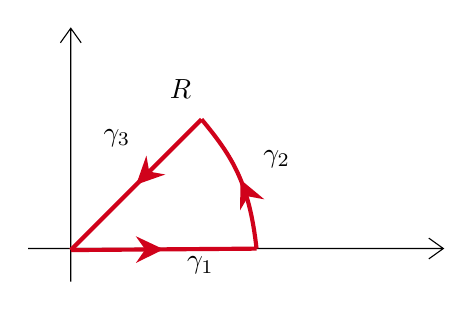
\begin{tikzpicture}[x=0.75pt,y=0.75pt,yscale=-1,xscale=1]
%uncomment if require: \path (0,176); %set diagram left start at 0, and has height of 176

%Shape: Axis 2D [id:dp035634818552425784] 
\draw  (200,140.05) -- (400,140.05)(220.5,33.92) -- (220.5,156) (393,135.05) -- (400,140.05) -- (393,145.05) (215.5,40.92) -- (220.5,33.92) -- (225.5,40.92)  ;
%Straight Lines [id:da7560460514537715] 
\draw [color={rgb, 255:red, 208; green, 2; blue, 27 }  ,draw opacity=1 ][line width=1.5]    (220.5,140.8) -- (283.5,77.8) ;
\draw [shift={(252,109.3)}, rotate = 315] [fill={rgb, 255:red, 208; green, 2; blue, 27 }  ,fill opacity=1 ][line width=0.08]  [draw opacity=0] (13.4,-6.43) -- (0,0) -- (13.4,6.44) -- (8.9,0) -- cycle    ;
%Curve Lines [id:da9635953000928117] 
\draw [color={rgb, 255:red, 208; green, 2; blue, 27 }  ,draw opacity=1 ][line width=1.5]    (283.5,77.8) .. controls (298.5,95.8) and (306.5,108.8) .. (310,140.11) ;
\draw [shift={(302.31,106.84)}, rotate = 65.41] [fill={rgb, 255:red, 208; green, 2; blue, 27 }  ,fill opacity=1 ][line width=0.08]  [draw opacity=0] (13.4,-6.43) -- (0,0) -- (13.4,6.44) -- (8.9,0) -- cycle    ;
%Straight Lines [id:da9987973908776102] 
\draw [color={rgb, 255:red, 208; green, 2; blue, 27 }  ,draw opacity=1 ][line width=1.5]    (220.5,140.8) -- (310,140.11) ;
\draw [shift={(265.25,140.45)}, rotate = 539.56] [fill={rgb, 255:red, 208; green, 2; blue, 27 }  ,fill opacity=1 ][line width=0.08]  [draw opacity=0] (13.4,-6.43) -- (0,0) -- (13.4,6.44) -- (8.9,0) -- cycle    ;

% Text Node
\draw (235,81.4) node [anchor=north west][inner sep=0.75pt]    {$\gamma _{3}$};
% Text Node
\draw (312,91.4) node [anchor=north west][inner sep=0.75pt]    {$\gamma _{2}$};
% Text Node
\draw (275.25,142.85) node [anchor=north west][inner sep=0.75pt]    {$\gamma _{1}$};
% Text Node
\draw (267,57.4) node [anchor=north west][inner sep=0.75pt]    {$R$};


\end{tikzpicture}
\end{figure}
\FloatBarrier

La funzione $f\left( z\right)$ è olomorfa, allora
\begin{equation*}
{\displaystyle \int\nolimits _{\gamma } f\left( z\right) dz=0=\int\nolimits _{\gamma _{1}} f\left( z\right) dz+\int\nolimits _{\gamma _{2}} f\left( z\right) dz+\int\nolimits _{\gamma _{3}} f}\left( z\right) dz
\end{equation*}
\begin{itemize}
\item La curva $\gamma _{3}$ ha parametrizzazione $z=re^{i\vartheta }$ con $r$ variabile e $\vartheta $ fissato. Il valore di $\vartheta $ si determina imponendo di potersi ricondurre all'integrale di Gauss, ovvero\begin{equation*}
iz^{2} =i\left( re^{i\vartheta }\right)^{2} =-r^{2} \ \ \Rightarrow \ \ \vartheta =\frac{\pi }{4}
\end{equation*}

Deduciamo il nuovo differenziale\begin{equation*}
z=re^{i\vartheta } \ \ \Rightarrow \ \ dz=e^{i\vartheta } dr=e^{i\frac{\pi }{4}} dr
\end{equation*}

Allora il terzo integrale diventa\begin{equation*}
\int\nolimits _{\gamma _{3}} e^{iz^{2}} dz=\int\nolimits ^{0}_{R} e^{-r^{2}} e^{i\frac{\pi }{4}} dr
\end{equation*}

Facciamo ora tendere $R\rightarrow +\infty $\begin{equation*}
\lim\limits _{R\rightarrow +\infty }\int\nolimits ^{0}_{R} e^{-r^{2}} e^{i\frac{\pi }{4}} dr=e^{i\frac{\pi }{4}}\lim\limits _{R\rightarrow +\infty }\int\nolimits ^{0}_{R} e^{-r^{2}} dr=-e^{i\frac{\pi }{4}}\int\nolimits ^{+\infty }_{0} e^{-r^{2}} dr=-e^{i\frac{\pi }{4}}\frac{\sqrt{\pi }}{2}
\end{equation*}
\item La curva $\gamma _{2}$ ha parametrizzazione $z=Re^{i\vartheta }$, con $R$ fissato e $\vartheta $ variabile in $\left[ 0,\frac{\pi }{4}\right]$. Deduciamo il nuovo differenziale\begin{equation*}
z=Re^{i\vartheta } \ \ \Rightarrow \ \ dz=Rie^{i\vartheta } d\vartheta 
\end{equation*}Il secondo integrale diventa

\begin{align*}
\int\nolimits _{\gamma _{2}} e^{iz^{2}} dz & =\int\nolimits ^{\pi /4}_{0} e^{iR^{2} e^{i2\vartheta }} Rie^{i\vartheta } d\vartheta \\
 & =\int\nolimits ^{\pi /4}_{0} iRe^{iR^{2} e^{i2\vartheta } +i\vartheta } d\vartheta \\
 & =\int\nolimits ^{\pi /4}_{0} iRe^{iR^{2}\left[\cos\left( 2\vartheta \right) +i\sin\left( 2\vartheta \right)\right] +i\vartheta } d\vartheta \\
 & =\int\nolimits ^{\pi /4}_{0} iRe^{iR^{2}\cos\left( 2\vartheta \right) -R^{2}\sin\left( 2\vartheta \right) +i\vartheta } d\vartheta \\
 & =\int\nolimits ^{\pi /4}_{0} iRe^{iR^{2}\cos\left( 2\vartheta \right)} e^{-R^{2}\sin\left( 2\vartheta \right)} e^{i\vartheta } d\vartheta 
\end{align*}

Poi\begin{align*}
\left| \int\nolimits _{\gamma _{2}} e^{iz^{2}} dz\right|  & =\left| \int\nolimits ^{\pi /4}_{0} iRe^{iR^{2}\cos\left( 2\vartheta \right)} e^{-R^{2}\sin\left( 2\vartheta \right)} e^{i\vartheta } d\vartheta \right| \\
 & \leqslant \int\nolimits ^{\pi /4}_{0}\left| i\right| \left| R\right| \left| e^{iR^{2}\cos\left( 2\vartheta \right)}\right| \left| e^{-R^{2}\sin\left( 2\vartheta \right)}\right| \left| e^{i\vartheta }\right| d\vartheta =R\int\nolimits ^{\pi /4}_{0} e^{-R^{2}\sin\left( 2\vartheta \right)} d\vartheta 
\end{align*}

Ricordando ora la seguente disugaglianza\begin{equation*}
\sin\left( 2\vartheta \right)  >\frac{4\vartheta }{\pi }
\end{equation*}

otteniamo\begin{equation*}
R\int\nolimits ^{\pi /4}_{0} e^{-R^{2}\sin\left( 2\vartheta \right)} d\vartheta \leqslant R\int\nolimits ^{\pi /4}_{0} e^{-R^{2}\frac{4\vartheta }{\pi }} d\vartheta =\left[ -\frac{\pi }{4R^{2}} e^{-R^{2}\frac{4\vartheta }{\pi }}\right]^{\pi /4}_{0} =\frac{\pi }{4R^{2}}\left( 1-e^{-R^{2}}\right)
\end{equation*}

la quale\begin{equation*}
\frac{\pi }{4R^{2}}\left( 1-e^{-R^{2}}\right)\xrightarrow{R\rightarrow +\infty } 0
\end{equation*}
\item La curva $\gamma _{1}$ ha parametrizzazione $z=x=R$, tuttavia non serve fare calcoli in quanto sappiamo che la somma dei tre integrali fa $0$ e ne abbiamo già calcolati due, pertanto\begin{equation*}
\int\nolimits _{\gamma _{1}} e^{iz^{2}} dz=-\int\nolimits _{\gamma _{3}} e^{iz^{2}} dz=e^{i\frac{\pi }{4}}\frac{\sqrt{\pi }}{2}
\end{equation*}
\end{itemize}

Notiamo a questo punto che l'integrale
\begin{equation*}
\int\nolimits _{\gamma _{1}} e^{iz^{2}} dz
\end{equation*}
non è altro che un integrale complesso, fatto però sulla curva $\gamma _{1}$, la quale coincide con la retta reale positiva. Di conseguenza
\begin{equation*}
\int\nolimits _{\gamma _{1}} e^{iz^{2}} dz=\int\nolimits ^{+\infty }_{0} e^{ix^{2}} dx
\end{equation*}
che sarà quindi una quantità complessa, ma l'integrale richiesto è proprio la parte reale di questa quantità
\begin{equation*}
\int\nolimits ^{+\infty }_{0}\cos\left( x^{2}\right) dx=\mathrm{Re}\left(\int\nolimits ^{+\infty }_{0} e^{ix^{2}} dz\right) =\mathrm{Re}\left( e^{i\frac{\pi }{4}}\frac{\sqrt{\pi }}{2}\right) =\cos\left(\frac{\pi }{4}\right)\frac{\sqrt{\pi }}{2} =\sqrt{\frac{\pi }{8}}
\end{equation*}
\chapter{Esercitazione 2 - Potrich}
\ParteEsercizi
\Esercizio{(Integrali di Fresnel)}

Calcolare
\begin{equation*}
\int\nolimits ^{+\infty }_{0}\cos t^{2} dt\ \ \ \ \ \ \ \ \int\nolimits ^{+\infty }_{0}\sin t^{2} dt
\end{equation*}
\Esercizio{}

Determinare l'anello di convergenza della seguente serie di Laurent
\begin{equation*}
f\left( z\right) =\sum\limits ^{\infty }_{n=-\infty }\frac{z^{2n}}{9^{\left| n\right| }}
\end{equation*}
\Esercizio{}

Determinare lo sviluppo di Laurent di
\begin{equation*}
f\left( z\right) =\frac{1}{2iz-z^{2}}
\end{equation*}
in
\begin{equation*}
A=\left\{z\in \mathbb{C} :0< \left| z\right| < 2\right\} \ \ \ \ \ \ \ \ B=\left\{z\in \mathbb{C} :\left| z-2i\right|  >2\right\}
\end{equation*}
\Esercizio{}

Determinare le singolarità e i residui.
\begin{equation*}
F\left( z\right) =\frac{1}{z-z^{3}} =\frac{1}{z\left( 1-z^{2}\right)} =\frac{1}{z\left( 1+z\right)\left( 1-z\right)}
\end{equation*}
\Esercizio{}

Determinare le singolarità e i residui.
\begin{equation*}
f\left( z\right) =\frac{z^{5}}{\left( 1+iz\right)^{2}}
\end{equation*}
\Esercizio{}

Determinare le singolarità e i residui.
\begin{equation*}
f\left( z\right) =\frac{e^{\frac{1}{z-1}}}{z^{2}\left( z^{2} +4\right)}
\end{equation*}
\Esercizio{}

Sia
\begin{equation*}
f\left( z\right) =\frac{e^{\frac{1}{z-1}}}{z-2}
\end{equation*}
\begin{enumerate}
\item Classificare le singolarità di $f$
\item Determinare la serie di Laurent centrata in $z=1$, precisandone l'insieme di convergenza
\item Calcolare i residui di $f$
\item Calcolare $\int _{\gamma } f\left( z\right) dz$ dove $\gamma :\left| z\right| =4$ percorsa in senso antiorario
\end{enumerate}
\ParteSoluzioni
\Soluzione

Si tratta di due integrali che convergono in senso improprio. Dimostriamolo:
\begin{equation*}
\int\nolimits ^{+\infty }_{0}\cos t^{2} dt=\left\{\begin{array}{ c }
t^{2} =x\\
t=\sqrt{x}\\
dt=\frac{1}{2\sqrt{x}} dx
\end{array}\right\} =\frac{1}{2}\int\nolimits ^{+\infty }_{0}\frac{\cos x}{\sqrt{x}} dx
\end{equation*}
Tale integrale converge in un intorno destro di $0$ in senso improprio. Studiamo ora la convergenza in un intorno di $+\infty $. Considerando le seguenti funzioni
\begin{equation*}
\begin{array}{ r l }
f\left( x\right) =\frac{1}{\sqrt{x}} & \rightarrow f'\left( x\right) =-\frac{1}{2x^{3/2}}\\
g\left( x\right) =\sin x & \rightarrow g'\left( x\right) =\cos x
\end{array}
\end{equation*}
possiamo integrare per parti
\begin{equation*}
\int\nolimits ^{a}_{1}\frac{\cos x}{\sqrt{x}} dx=\left[\frac{\sin x}{\sqrt{x}}\right]^{a}_{1} +\int\nolimits ^{a}_{1}\frac{\sin x}{2x^{3/2}} dx=\frac{\sin a}{\sqrt{a}} -\sin 1+\int\nolimits ^{a}_{1}\frac{\sin x}{2x^{3/2}} dx
\end{equation*}
che per $a\rightarrow +\infty $ tende a
\begin{equation*}
-\sin 1+\int\nolimits ^{+\infty }_{1}\frac{\sin x}{2x^{3/2}} dx
\end{equation*}
dobbiamo quindi studiare la convergenza di tale integrale.
\begin{nb}
Convergenza di integrali.
\begin{gather*}
\int\nolimits ^{+\infty }_{1}\frac{1}{x^{\alpha }} dx\ \ \text{converge} \ \ \Leftrightarrow \ \ \alpha  >1\\
\int\nolimits ^{1}_{0}\frac{1}{x^{\alpha }} dx\ \ \text{converge} \ \ \Leftrightarrow \ \ \alpha < 1
\end{gather*}
\end{nb}
Pertanto
\begin{equation*}
\left| \int\nolimits ^{+\infty }_{1}\frac{\sin x}{2x^{3/2}} dx\right| \leqslant \int\nolimits ^{+\infty }_{1}\left| \frac{\sin x}{2x^{3/2}}\right| dx\leqslant \int\nolimits ^{+\infty }_{1}\frac{1}{2x^{3/2}} dx
\end{equation*}
in cui $\alpha =3/2 >1$, pertanto converge.

Calcoliamo
\begin{equation*}
J=\int\nolimits ^{+\infty }_{0} e^{it^{2}} dt=\int\nolimits ^{+\infty }_{0}\cos t^{2} dt+i\int\nolimits ^{+\infty }_{0}\sin t^{2} dt
\end{equation*}
Poniamo
\begin{equation*}
f\left( z\right) =e^{iz^{2}} \in \mathcal{H}\left(\mathbb{C}\right)
\end{equation*}
Consideriamo una curva $\gamma =\gamma _{1} \cup \gamma _{2} \cup \gamma _{3}$ fatta come


\begin{figure}[htpb]
	\centering
\tikzset{every picture/.style={line width=0.75pt}} %set default line width to 0.75pt        

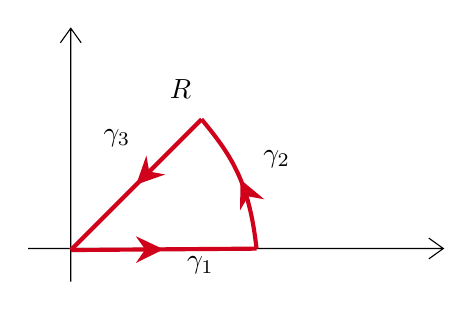
\begin{tikzpicture}[x=0.75pt,y=0.75pt,yscale=-1,xscale=1]
%uncomment if require: \path (0,176); %set diagram left start at 0, and has height of 176

%Shape: Axis 2D [id:dp17170898643653087] 
\draw  (220,126.6) -- (420,126.6)(240.5,20.47) -- (240.5,142.55) (413,121.6) -- (420,126.6) -- (413,131.6) (235.5,27.47) -- (240.5,20.47) -- (245.5,27.47)  ;
%Straight Lines [id:da9725409241349892] 
\draw [color={rgb, 255:red, 208; green, 2; blue, 27 }  ,draw opacity=1 ][line width=1.5]    (240.5,127.34) -- (303.5,64.34) ;
\draw [shift={(272,95.84)}, rotate = 315] [fill={rgb, 255:red, 208; green, 2; blue, 27 }  ,fill opacity=1 ][line width=0.08]  [draw opacity=0] (13.4,-6.43) -- (0,0) -- (13.4,6.44) -- (8.9,0) -- cycle    ;
%Curve Lines [id:da9846937875734199] 
\draw [color={rgb, 255:red, 208; green, 2; blue, 27 }  ,draw opacity=1 ][line width=1.5]    (303.5,64.34) .. controls (318.5,82.34) and (326.5,95.34) .. (330,126.66) ;
\draw [shift={(322.31,93.38)}, rotate = 65.41] [fill={rgb, 255:red, 208; green, 2; blue, 27 }  ,fill opacity=1 ][line width=0.08]  [draw opacity=0] (13.4,-6.43) -- (0,0) -- (13.4,6.44) -- (8.9,0) -- cycle    ;
%Straight Lines [id:da17260088434526732] 
\draw [color={rgb, 255:red, 208; green, 2; blue, 27 }  ,draw opacity=1 ][line width=1.5]    (240.5,127.34) -- (330,126.66) ;
\draw [shift={(285.25,127)}, rotate = 539.56] [fill={rgb, 255:red, 208; green, 2; blue, 27 }  ,fill opacity=1 ][line width=0.08]  [draw opacity=0] (13.4,-6.43) -- (0,0) -- (13.4,6.44) -- (8.9,0) -- cycle    ;

% Text Node
\draw (255,67.95) node [anchor=north west][inner sep=0.75pt]    {$\gamma _{3}$};
% Text Node
\draw (332,77.95) node [anchor=north west][inner sep=0.75pt]    {$\gamma _{2}$};
% Text Node
\draw (295.25,129.4) node [anchor=north west][inner sep=0.75pt]    {$\gamma _{1}$};
% Text Node
\draw (287,43.95) node [anchor=north west][inner sep=0.75pt]    {$R$};


\end{tikzpicture}
\end{figure}
\FloatBarrier

le cui parti sono parametrizzate come segue
\begin{itemize}
\item $\gamma _{1}\left( t\right) =t$ con $t\in \left[ 0,R\right]$
\item $\gamma _{2}\left( t\right) =Re^{it}$ con $t\in \left[ 0,\frac{\pi }{4}\right]$
\item $-\gamma _{3}\left( t\right) =te^{i\frac{\pi }{4}}$ con $t\in \left[ 0,R\right]$
\end{itemize}

Analizziamo cosa succede all'integrale di $f\left( z\right)$ sui vari percorsi
\begin{itemize}
\item su $\gamma _{1}$\begin{equation*}
\int\nolimits _{\gamma _{1}} f\left( z\right) dz=\int\nolimits ^{R}_{0} e^{it^{2}} dt\xrightarrow{R\rightarrow +\infty }\int\nolimits ^{+\infty }_{0} e^{it^{2}} dt=J
\end{equation*}
\item su $\gamma _{3}$\begin{align*}
\int\nolimits _{\gamma _{3}} f\left( z\right) dz & =-\int\nolimits ^{R}_{0} f\left( \gamma \left( t\right)\right) \gamma '\left( t\right) dt=-\int\nolimits ^{R}_{0} e^{it^{2} e^{i\frac{\pi }{2}}} e^{i\frac{\pi }{4}} dt\\
 & =-\int\nolimits ^{R}_{0} e^{it^{2} i} e^{i\frac{\pi }{4}} dt=-e^{i\frac{\pi }{4}}\int\nolimits ^{R}_{0} e^{-t^{2}} dt\xrightarrow{R\rightarrow +\infty } -e^{i\frac{\pi }{4}}\int\nolimits ^{+\infty }_{0} e^{-t^{2}} dt
\end{align*}

\begin{nb}
Ricordiamo l'integrale di Gauss
\begin{equation*}
\int\nolimits _{\mathbb{R}} e^{-x^{2}} dx=\sqrt{\pi }
\end{equation*}
\end{nb}

Otteniamo che\begin{equation*}
\int\nolimits _{\gamma _{3}} f\left( z\right) dz\xrightarrow{R\rightarrow +\infty } -e^{i\frac{\pi }{4}}\frac{\sqrt{\pi }}{2}
\end{equation*}
\item su $\gamma _{2}$ dobbiamo cercare una maggiorazione in modo da far vedere che tende a $0$. Ricordiamo anche che $\left| e^{z}\right| =e^{\mathrm{Re}\left( z\right)}$\begin{align*}
0 & \leqslant \left| \int\nolimits _{\gamma _{2}} f\left( z\right) dz\right| =\left| \int\nolimits ^{\pi /4}_{0} f\left( \gamma \left( t\right)\right) \gamma '\left( t\right) dt\right| =\left| \int\nolimits ^{\pi /4}_{0} e^{iR^{2} e^{2it}} Rie^{it} dt\right| \\
 & \leqslant R\int\nolimits ^{\pi /4}_{0}\left| e^{iR^{2} e^{2it}}\right| dt=R\int\nolimits ^{\pi /4}_{0}\left| e^{iR^{2} e^{2it}}\right| dt=R\int\nolimits ^{\pi /4}_{0} e^{\mathrm{Re}\left[ iR^{2}\left(\cos\left( 2t\right) +i\sin\left( 2t\right)\right)\right]} dt\\
 & =R\int\nolimits ^{\pi /4}_{0} e^{-R^{2}\sin\left( 2t\right)} dt=\left\{\begin{array}{ c }
2t=x\\
dt=\frac{dx}{2}
\end{array}\right\} =\frac{R}{2}\int\nolimits ^{\pi /2}_{0} e^{-R^{2}\sin x} dx
\end{align*}

minoriamo ora il seno



\begin{figure}[htpb]
	\centering
\tikzset{every picture/.style={line width=0.75pt}} %set default line width to 0.75pt        

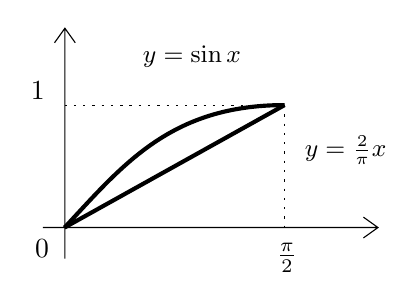
\begin{tikzpicture}[x=0.75pt,y=0.75pt,yscale=-1,xscale=1]
%uncomment if require: \path (0,140); %set diagram left start at 0, and has height of 140

%Shape: Axis 2D [id:dp521862829598075] 
\draw  (200,100.03) -- (361.5,100.03)(210.67,4) -- (210.67,115.03) (354.5,95.03) -- (361.5,100.03) -- (354.5,105.03) (205.67,11) -- (210.67,4) -- (215.67,11)  ;
%Curve Lines [id:da7711478785582004] 
\draw [line width=1.5]    (210.5,100.03) .. controls (238.5,70.03) and (261.5,41.03) .. (316.5,41.03) ;
%Straight Lines [id:da5280090308997825] 
\draw  [dash pattern={on 0.84pt off 2.51pt}]  (210.5,41.03) -- (316.5,41.03) ;
%Straight Lines [id:da665885556586004] 
\draw  [dash pattern={on 0.84pt off 2.51pt}]  (316.5,41.03) -- (316.5,100.03) ;
%Straight Lines [id:da2630936419717216] 
\draw [line width=1.5]    (316.5,41.03) -- (210.5,100.03) ;

% Text Node
\draw (193,28.4) node [anchor=north west][inner sep=0.75pt]    {$1$};
% Text Node
\draw (311.5,106.43) node [anchor=north west][inner sep=0.75pt]    {$\frac{\pi }{2}$};
% Text Node
\draw (195,104.4) node [anchor=north west][inner sep=0.75pt]    {$0$};
% Text Node
\draw (325,54.4) node [anchor=north west][inner sep=0.75pt]  [font=\small]  {$y=\frac{2}{\pi } x$};
% Text Node
\draw (247,11.4) node [anchor=north west][inner sep=0.75pt]  [font=\small]  {$y=\sin x$};


\end{tikzpicture}
\end{figure}
\FloatBarrier


otteniamo\begin{align*}
\frac{R}{2}\int\nolimits ^{\pi /2}_{0} e^{-R^{2}\sin x} dx & \leqslant \frac{R}{2}\int\nolimits ^{\pi /2}_{0} e^{-\frac{2}{\pi } R^{2} x} dx\\
 & =\frac{R}{2}\left[ -\frac{\pi }{2R^{2}} e^{-\frac{2R^{2}}{\pi } x}\right]^{\pi /2}_{0} =\frac{\pi }{4R}\left( 1-e^{-R^{2}}\right)\xrightarrow{R\rightarrow +\infty } 0
\end{align*}
\end{itemize}

Per il teorema dell'integrale nullo di Cauchy
\begin{equation*}
0=\oint\nolimits _{\gamma } f\left( z\right) dz=\int\nolimits _{\gamma _{1}} f\left( z\right) dz+\int\nolimits _{\gamma _{2}} f\left( z\right) dz+\int\nolimits _{\gamma _{3}} f\left( z\right) dz
\end{equation*}
sostituiamo i vari elementi, sempre per $R\rightarrow +\infty $
\begin{equation*}
0=J+0-e^{i\frac{\pi }{4}}\frac{\sqrt{\pi }}{2}
\end{equation*}
allora
\begin{equation*}
J=\int\nolimits ^{+\infty }_{0} e^{it^{2}} dt=e^{i\frac{\pi }{4}}\frac{\sqrt{\pi }}{2} =\frac{\sqrt{2\pi }}{4}\left( 1+i\right)
\end{equation*}
ma quindi
\begin{align*}
\int\nolimits ^{+\infty }_{0}\cos t^{2} dt & =\mathrm{Re}\left( J\right) =\frac{\sqrt{2\pi }}{4}\\
\int\nolimits ^{+\infty }_{0}\sin t^{2} dt & =\mathrm{Im}\left( J\right) =\frac{\sqrt{2\pi }}{4}
\end{align*}
\Soluzione
\begin{align*}
f\left( z\right) = & \sum\limits ^{\infty }_{n=-\infty }\frac{z^{2n}}{9^{\left| n\right| }} =\sum _{n< 0}\frac{z^{2n}}{9^{\left| n\right| }} +\sum _{n\geqslant 0}\frac{z^{2n}}{9^{n}}\\
 & =\sum _{n >0}\frac{z^{-2n}}{9^{n}} +\sum _{n\geqslant 0}\frac{z^{2n}}{9^{n}}\\
 & =\sum _{n >0}\frac{1}{9^{n} z^{2n}} +\sum _{n\geqslant 0}\frac{z^{2n}}{9^{n}}
\end{align*}
Affinché la serie di Laurent converga devono convergere entrambe le serie. La prima converge se
\begin{equation*}
\lim\limits _{n\rightarrow \infty }\left| \frac{a_{n+1}}{a_{n}}\right| =\lim\limits _{n\rightarrow \infty }\frac{9^{n}\left| z\right| ^{2n}}{9^{n+1}\left| z\right| ^{2\left( n+1\right)}} =\frac{1}{9\left| z\right| ^{2}} < 1
\end{equation*}
ossia $\left| z\right| ^{2}  >\frac{1}{9}$, cioè $\left| z\right|  >\frac{1}{3}$.

La seconda serie converge se
\begin{equation*}
\lim\limits _{n\rightarrow \infty }\left| \frac{b_{n+1}}{b_{n}}\right| =\lim\limits _{n\rightarrow \infty }\frac{\left| z\right| ^{2\left( n+1\right)}}{9^{n+1}}\frac{9^{n}}{\left| z\right| ^{2n}} =\frac{1}{9}\left| z\right| ^{2} < 1
\end{equation*}
ossia $\left| z\right| ^{2} < 9$, cioè $\left| z\right| < 3$.

Allora l'anello di convergenza è $A=\left\{z\in \mathbb{C} :\frac{1}{3} < \left| z\right| < 3\right\}$.
\Soluzione

Possiamo vedere la $f$ come
\begin{equation*}
f\left( z\right) =\frac{1}{2iz-z^{2}} =\frac{1}{z\left( 2i-z\right)} =\frac{1}{z} \cdotp \frac{1}{2i} \cdotp \frac{1}{1-\frac{z}{2i}}
\end{equation*}
In $A$
\begin{align*}
f\left( z\right) & =\frac{1}{z} \cdotp \frac{1}{2i} \cdotp \frac{1}{1-\frac{z}{2i}} =\frac{1}{z} \cdotp \frac{1}{2i} \cdotp \sum\limits ^{\infty }_{n=0}\frac{z^{n}}{\left( 2i\right)^{n}}\\
 & =\sum\limits ^{\infty }_{n=0}\frac{z^{n-1}}{\left( 2i\right)^{n+1}} =\sum\limits ^{\infty }_{n=-1}\frac{z^{n}}{\left( 2i\right)^{n+2}}
\end{align*}
In $B$
\begin{align*}
f\left( z\right) & =\frac{1}{z\left( 2i-z\right)} =\frac{A}{z} +\frac{B}{2i-z} =\frac{A2i-Az+Bz}{z\left( 2i-z\right)} =\frac{A2i+z\left( B-A\right)}{z\left( 2i-z\right)}
\end{align*}
allora $A=B=-\frac{i}{2}$
\begin{align*}
f\left( z\right) & =-\frac{i}{2}\left\{\frac{1}{z} +\frac{1}{2i-z}\right\}\\
 & =-\frac{i}{2}\left\{\frac{1}{\left( z-2i\right) +2i} +\frac{1}{2i-z}\right\}\\
 & =-\frac{i}{2}\left\{\frac{1}{z-2i} \cdotp \frac{1}{1+\frac{2i}{z-2i}} +\frac{1}{2i-z}\right\}\\
 & =-\frac{i}{2}\left\{\frac{1}{z-2i} \cdotp \frac{1}{1-\frac{-2i}{z-2i}} -\frac{1}{z-2i}\right\}
\end{align*}
Essendo in $B$
\begin{equation*}
\left| \frac{-2i}{z-2i}\right| < 1\ \ \Leftrightarrow \ \ 2< \left| z-2i\right| 
\end{equation*}
possiamo scrivere la serie geometrica
\begin{align*}
f\left( z\right) & =-\frac{i}{2}\left\{\frac{1}{z-2i} \cdotp \sum\limits ^{\infty }_{n=0}\left(\frac{-2i}{z-2i}\right)^{n} -\frac{1}{z-2i}\right\}\\
 & =-\frac{i}{2}\left\{\frac{1}{z-2i}\left[\sum\limits ^{\infty }_{n=0}\left(\frac{-2i}{z-2i}\right)^{n} -1\right]\right\}\\
 & =-\frac{i}{2}\left\{\frac{1}{z-2i}\sum\limits ^{\infty }_{n=1}\left(\frac{-2i}{z-2i}\right)^{n}\right\}\\
 & =-\frac{i}{2}\left\{\sum\limits ^{\infty }_{n=1}\frac{\left( -2i\right)^{n}}{\left( z-2i\right)^{n+1}}\right\}
\end{align*}
\Soluzione
\begin{theorem}
Sia $f\in \mathcal{H}\left( D\left( z_{0} ,R\right) \setminus \left\{z_{0}\right\}\right)$, cioè $z_{0}$ è una \textbf{singolarità isolata} per $f$. Allora localmente
\begin{equation*}
f\left( z\right) =\sum\limits ^{+\infty }_{n=-\infty } a_{n}\left( z-z_{0}\right)^{n}
\end{equation*}
\end{theorem}
\begin{theorem}
Sia $M=\left\{n\in \mathbb{Z} :n< 0,a_{n} \neq 0\right\}$ l'insieme degli indici della parte singolare dello sviluppo di Laurent. $z_{0}$ è

\begin{itemize}
\item \textbf{singolarità eliminabile} se

\begin{equation*}
\exists \lim\limits _{z\rightarrow z_{0}} f\left( z\right) \in \mathbb{C} \ \ \Leftrightarrow \ \ M=\emptyset \ \ \Leftrightarrow \ \ f\ \text{è limitata su} \ \mathcal{U}\left( z_{0}\right)
\end{equation*}
\item \textbf{polo} se

\begin{equation*}
\exists \lim\limits _{z\rightarrow z_{0}} f\left( z\right) =\infty \ \ \Leftrightarrow \ \ 0< \left| M\right| < +\infty 
\end{equation*}

dove $-\min M=k$ è l'\textbf{ordine} del polo.
\item \textbf{singolarità essenziale} se

\begin{gather*}
\nexists \lim\limits _{z\rightarrow z_{0}} f\left( z\right) \ \ \Leftrightarrow \ \ \left| M\right| =\infty \\
\Leftrightarrow \ \ \forall \varepsilon \in \left( 0,R\right) \ \text{l'insieme immagine} \ f\left(\left\{0< \left| z-z_{0}\right| < \varepsilon \right\}\right) \ \text{è denso in} \ \mathbb{C}
\end{gather*}
\end{itemize}
\end{theorem}
\begin{definition}
Si dice residuo di $f$ in $z_{0}$
\begin{equation*}
\mathrm{Res}\left( f,z_{0}\right) :=a_{-1}
\end{equation*}
\end{definition}
\begin{theorem}
Sia $f\in \mathcal{H}\left(\mathbb{C} \setminus \overline{D\left( z_{0} ,R\right)}\right)$ ed $M=\left\{n\in \mathbb{Z} :n >0,a_{n} \neq 0\right\}$. Il punto $\infty $ è

\begin{itemize}
\item \textbf{singolarità eliminabile} se e solo se\begin{equation*}
\exists \lim\limits _{z\rightarrow \infty } f\left( z\right) \in \mathbb{C} \ \ \Leftrightarrow \ \ M=\emptyset 
\end{equation*}
\item \textbf{polo} se e solo se\begin{equation*}
\exists \lim\limits _{z\rightarrow \infty } f\left( z\right) =\infty \ \ \Leftrightarrow \ \ 0< \left| M\right| < \infty 
\end{equation*}
\item \textbf{singolarità essenziale} se e solo se\begin{equation*}
\nexists \lim\limits _{z\rightarrow +\infty } f\left( z\right) \ \ \Leftrightarrow \ \ \left| M\right| =\infty 
\end{equation*}
\end{itemize}
\end{theorem}
\begin{definition}
Si dice residuo di $f$ in $\infty $
\begin{equation*}
\mathrm{Res}\left( f,\infty \right) :=-a_{-1}
\end{equation*}
\end{definition}
\begin{theorem}
[di De l'Hôpital] Siano $f$ e $g$ funzioni analitiche in $B_{R}\left( z_{0}\right)$ tali che $f\left( z_{0}\right) =g\left( z_{0}\right) =0$ e $g'\left( z_{0}\right) \neq 0$ (quindi solo la forma $\frac{0}{0}$ al finito). Allora
\begin{equation*}
\lim\limits _{z\rightarrow z_{0}}\frac{f\left( z\right)}{g\left( z\right)} =\frac{f'\left( z_{0}\right)}{g'\left( z_{0}\right)}
\end{equation*}
\end{theorem}
\begin{theorem}
Le seguenti affermazioni sono equivalenti
\begin{itemize}
\item $f$ ha in $z_{0}$ un polo di ordine $m$
\item $g\left( z\right) =\left( z-z_{0}\right)^{m} f\left( z\right)$ ha in $z_{0}$ una singolarità eliminabile e $\lim\limits _{z\rightarrow z_{0}} g\left( z\right) \neq 0$
\item $f\left( z\right) \approx \left| z-z_{0}\right| ^{m}$ per $z\rightarrow z_{0}$
\item $\frac{1}{f\left( z\right)}$ ha in $z_{0}$ uno zero di ordine $m$
\end{itemize}
\end{theorem}
\begin{theorem}
Siano $f(z)$ e $g(z)$ tali che $f\left( z_{0}\right) =0=g\left( z_{0}\right)$ e siano $n$ ed $m$ rispettivamente, gli ordini di $z_{0}$ come zero di $f$ e $g$. La funzione $\frac{f(z)}{g(z)}$ ha in $z_{0}$:

\begin{itemize}
\item una singolarità eliminabile che è uno zero d'ordine $n-m$ se e solo se $n >m$
\item una singolarità eliminabile che non è uno zero se e solo se $n=m$
\item un polo d'ordine $m-n$ se e solo se $m >n$.
\end{itemize}
\end{theorem}
\begin{theorem}
Sia $f\in \mathcal{H}\left(\mathbb{C} \setminus \left\{z_{1} ,\dotsc ,z_{n}\right\}\right)$ allora
\begin{equation*}
\sum\limits ^{n}_{k=1}\mathrm{Res}\left( f,z_{k}\right) +\mathrm{Res}\left( f,\infty \right) =0
\end{equation*}
\end{theorem}
\begin{theorem}
Sia $f\in \mathcal{H}\left(\mathbb{C} \setminus \left\{z_{1} ,\dotsc ,z_{n}\right\}\right)$. Se $R >\max_{1\leqslant k\leqslant n}\left| z_{k}\right| $ allora
\begin{equation*}
\int\nolimits _{\partial D\left( 0,R\right)} f\left( z\right) dz=2\pi i\left[\sum\limits ^{n}_{k=1}\mathrm{Res}\left( f,z_{k}\right)\right]
\end{equation*}
\end{theorem}
\begin{nb}
Come si calcolano i residui?
Nei punti all'infinito si definisce
\begin{equation*}
\mathrm{Res}\left( f,\infty \right) =\mathrm{Res}\left( -\frac{1}{z^{2}} f\left(\frac{1}{z}\right) ,0\right)
\end{equation*}
Nei punti $z_{0} \neq \infty $
\begin{enumerate}
\item se è una singolarità eliminabile:\begin{equation*}
\mathrm{Res}\left( f,z_{0}\right) =0
\end{equation*}

(attenzione: solo per i punti finiti)
\item se è un polo, c'è la \textbf{formula dei poli}
\begin{enumerate}
\item semplice (di ordine $p=1$)\begin{equation*}
\mathrm{Res}\left( f,z_{0}\right) =\lim\limits _{z\rightarrow z_{0}} f\left( z\right)\left( z-z_{0}\right)
\end{equation*}
\item di ordine $p\geqslant 2$\begin{equation*}
\mathrm{Res}\left( f,z_{0}\right) =\frac{1}{\left( p-1\right) !}\lim\limits _{z\rightarrow z_{0}}\left\{\frac{d^{p-1}}{dz^{p-1}}\left[ f\left( z\right)\left( z-z_{0}\right)^{p}\right]\right\}
\end{equation*}
\end{enumerate}
\item se è una singolarità essenziale bisogna per forza fare lo sviluppo di Laurent (che è valido in tutti i casi in realtà, ma è decisamente più laborioso la maggior parte delle volte)
\end{enumerate}
\end{nb}
\begin{theorem}
Sia $F=\frac{f}{g}$. Se $f\in \mathcal{H}\left(\mathcal{U}\left( z_{0}\right)\right)$ e $g$ ha in $z_{0}$ uno zero semplice ($g\left( z_{0}\right) =0$ e $g'\left( z_{0}\right) \neq 0$), allora\begin{equation*}
\mathrm{Res}\left(\frac{f}{g} ,z_{0}\right) =\frac{f\left( z_{0}\right)}{g'\left( z_{0}\right)}
\end{equation*}

Ricordiamo che se $f$ non si annulla in $z_{0}$ allora $F$ ha in $z_{0}$ un polo del I ordine. Se $f$ si annulla in $z_{0}$ allora $F$ ha in $z_{0}$ una singolarità eliminabile.
\end{theorem}
Le singolarità isolate sono $0,1,-1,\infty $.

$z=0,z=1,z=-1$ annullano il denominatore con molteplicità $1$ e non annullano il numeratore, quindi sono degli $1$-poli. Per il teorema appena enunciato:
\begin{gather*}
\mathrm{Res}\left( F,0\right) =\left\{g\left( z\right) =z,\ f\left( z\right) =\frac{1}{1-z^{2}}\right\} =\frac{1}{1} =1\\
\mathrm{Res}\left( F,1\right) =\left\{g\left( z\right) =1-z,\ f\left( z\right) =\frac{1}{z\left( 1+z\right)}\right\} =\frac{\frac{1}{2}}{-1} =-\frac{1}{2}\\
\mathrm{Res}\left( F,-1\right) =\left\{g\left( z\right) =1+z,\ f\left( z\right) =\frac{1}{z\left( 1-z\right)}\right\} =-\frac{1}{2}
\end{gather*}
Mentre
\begin{equation*}
F\left( z\right) =\frac{1}{z\left( 1+z\right)\left( 1-z\right)} \sim \frac{1}{z^{3}} \ \ \ \ z\rightarrow +\infty 
\end{equation*}
quindi $\infty $ è una singolarità eliminabile.
\begin{equation*}
\mathrm{Res}\left( F,\infty \right) =-\sum\limits ^{3}_{k=1}\mathrm{Res}\left( F,z_{k}\right) =-\left( 1-\frac{1}{2} -\frac{1}{2}\right) =0
\end{equation*}
\begin{oss}
Se $\infty $ è singolarità eliminabile, ciò non implica per forza $\mathrm{Res}\left( f,\infty \right) =0$. Infatti $f\left( z\right) =\frac{1}{z}\rightarrow 0$ per $z\rightarrow +\infty $ quindi $\infty $ è singolarità eliminabile, ma $\mathrm{Res}\left( f,\infty \right) =-a_{-1} =-1\neq 0$.
\end{oss}
\begin{nb}
Nel nostro caso è vero perchè vale il seguente teorema.
\end{nb}
\begin{theorem}
Se $f$ ha uno zero di ordine almeno $2$ in $\infty $ allora $\mathrm{Res}\left( f,\infty \right) =0$, perché
\begin{equation*}
f\left( z\right) =\sum\limits ^{2}_{n=-\infty } a_{n} z^{n} \ \ \Rightarrow \ \ \mathrm{Res}\left( f,\infty \right) =-a_{-1} =0
\end{equation*}
\end{theorem}
\Soluzione

Le singolarità isolate di $f$ sono $i,\infty $.

$z=i$ annulla il denominatore con molteplicità $2$ e non annulla il numeratore, quindi è un polo. Usando la formula dei poli
\begin{equation*}
\mathrm{Res}\left( f,i\right) =\frac{d}{dz} f\left( z\right)\left( z-i\right)^{2} =\left. -5z^{4}\right| _{z=i} =-5
\end{equation*}
$f\left( z\right) \sim -z^{3}$ per $z\rightarrow +\infty $ quindi $\infty $ è un $3$-polo.
\begin{equation*}
\mathrm{Res}\left( f,\infty \right) =-\mathrm{Res}\left( f,i\right) =5
\end{equation*}
\Soluzione

Le singolarità isolate di $f$ sono $1,0,\pm 2i,\infty $.

$z=\pm 2i$ sono zeri di molteplicità $1$ per il denominatore di $f$ e non annullano il denominatore, quindi sono $1$-poli. Usando la formula dei poli
\begin{gather*}
\mathrm{Res}\left( f,2i\right) =\lim\limits _{z\rightarrow 2i}\left( z-2i\right) f\left( z\right) =\dotsc =\frac{e^{-\frac{1+2i}{5}}}{16} i\\
\mathrm{Res}\left( f,-2i\right) =\lim\limits _{z\rightarrow -2i}\left( z+2i\right) f\left( z\right) =\dotsc =-\frac{e^{\frac{2i-1}{5}}}{16} i
\end{gather*}
$z=0$ è uno zero di molteplicità $2$ per il denominatore di $f$ e non annulla il denominatore, quindi è un $2$-polo. Usando la formula dei poli
\begin{equation*}
\mathrm{Res}\left( f,0\right) =\lim\limits _{z\rightarrow 0}\frac{d}{dz} z^{2} f\left( z\right) =\dotsc =-\frac{1}{4e}
\end{equation*}
$z=1$ è una singolarità essenziale perché $\nexists \lim\limits _{z\rightarrow 1} f\left( z\right)$.

Abbiamo che $f\left( z\right) \sim \frac{e}{z^{4}}$ per $z\rightarrow +\infty $, allora per il teorema $\mathrm{Res}\left( f,\infty \right) =0$.

Infine
\begin{equation*}
\mathrm{Res}\left( f,1\right) =-\sum \mathrm{Res}\left( f,\dotsc \right) =\frac{1}{4e} -\frac{\sin\left(\frac{2}{5}\right)}{8e^{\frac{1}{5}}}
\end{equation*}
\Soluzione
\begin{enumerate}
\item Le singolarità di $f$ sono $1,2,\infty $.

$z=1$ è singolarità essenziale perché $\nexists \lim\limits _{z\rightarrow 1} f\left( z\right)$

$z=2$ è $1$-polo perché annulla il denominatore con molteplicità $1$ e non annulla il numeratore.

$z=\infty $ è singolarità eliminabile perché $\exists \lim\limits _{z\rightarrow \infty } f\left( z\right) \in \mathbb{C}$.
\item Ricordiamo che

\begin{nb}
\begin{equation*}
e^{z} =\sum\limits ^{\infty }_{n=0}\frac{z^{n}}{n!} ,\ \ z\in \mathbb{C} \ \ \ \ \ \ \ \ \frac{1}{1-z} =\sum\limits ^{\infty }_{n=0} z^{n} ,\ \ \left| z\right| < 1
\end{equation*}
\end{nb}

Qui\begin{equation*}
e^{\frac{1}{z-1}} =\sum\limits ^{\infty }_{h=0}\frac{1}{h!\left( z-1\right)^{h}}
\end{equation*}mentre\begin{equation*}
\frac{1}{z-2} =-\frac{1}{2-z} =-\frac{1}{1-\left( z-1\right)} =-\sum\limits ^{\infty }_{k=0}\left( z-1\right)^{k}
\end{equation*}La prima serie converge in $\left| z-1\right|  >0$ e la seconda in $\left| z-1\right| < 1$. La serie di Laurent converge quindi in $0< \left| z-1\right| < 1$.\begin{nb}
Per scrivere la serie di Laurent sfruttiamo il prodotto alla Cauchy.
\begin{equation*}
\left(\sum\limits ^{\infty }_{n=0} a_{n}\right)\left(\sum\limits ^{\infty }_{n=0} b_{n}\right) =\sum\limits ^{\infty }_{n=0}\left(\sum\limits ^{n}_{k=0} a_{k} b_{n-k}\right)
\end{equation*}
\end{nb}Quindi\begin{equation*}
f\left( z\right) =-\sum\limits ^{\infty }_{k=0}\sum\limits ^{k}_{h=0}\frac{\left( z-1\right)^{k-2h}}{h!}
\end{equation*}
\item $\mathrm{Res}\left( f,2\right) =e$ per la formula dei poli

$\mathrm{Res}\left( f,1\right) =a_{-1}$ lo trovo ponendo $k-2h=-1$, quindi $a_{-1} =-\sum\limits ^{\infty }_{h=1}\frac{1}{h!} =1-e$

$\mathrm{Res}\left( f,\infty \right) =-1$
\item Applico il teorema dei residui\begin{equation*}
\int\nolimits _{\gamma } f\left( z\right) dz=2\pi i\left[\mathrm{Res}\left( f,1\right) +\mathrm{Res}\left( f,2\right)\right] =2\pi i
\end{equation*}
\end{enumerate}
\chapter{Esercitazione 3 - Boella}
\ParteEsercizi
\Esercizio{}

Calcolare il seguente integrale
\begin{equation*}
\int _{\mathbb{R}}\frac{1}{x^{4} +4a^{4}} dx
\end{equation*}
\Esercizio{}

Calcolare il seguente integrale
\begin{equation*}
\int _{\mathbb{R}}\frac{e^{-i\lambda x}}{x^{6} +64} dx\ \ \ \ \forall \lambda \in \mathbb{R}
\end{equation*}
\Esercizio{}

Calcolare il seguente integrale
\begin{equation*}
\int ^{\pi }_{0}\frac{1}{a+b\cos \vartheta } d\vartheta \ \ \ \ 0< b< a
\end{equation*}
\Esercizio{}

Calcolare il seguente integrale, per i valori di $\alpha $ in cui converge
\begin{equation*}
\int _{\mathbb{R}}\frac{e^{\alpha x}}{1+e^{x}} dx\ \ \ \ \alpha \in \mathbb{R}
\end{equation*}
\Esercizio{}

Calcolare il seguente integrale
\begin{equation*}
\int ^{+\infty }_{0}\frac{\cos\left( \alpha x\right)}{x^{2} +\beta ^{2}} dx\ \ \ \ \alpha \neq 0,\beta \neq 0
\end{equation*}
\ParteSoluzioni
\Soluzione

Per cominciare pensiamo il nostro integrale come
\begin{equation*}
\int _{\mathbb{R}}\frac{1}{x^{4} +4a^{4}} dx=\lim\limits _{R\rightarrow +\infty }\int ^{R}_{-R}\frac{1}{x^{4} +4a^{4}} dx
\end{equation*}
Consideriamo un percorso $\gamma _{R}$ fatto dall'unione della curva da $-R$ a $R$ e la semicirconferenza di raggio $R$ che chiameremo $\sigma _{R}$


\begin{figure}[htpb]
	\centering
\tikzset{every picture/.style={line width=0.75pt}} %set default line width to 0.75pt        

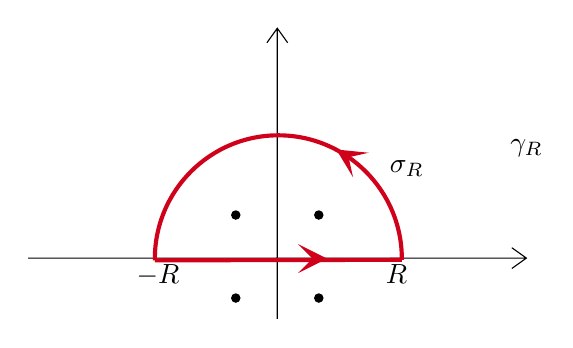
\begin{tikzpicture}[x=0.75pt,y=0.75pt,yscale=-1,xscale=1]
%uncomment if require: \path (0,179); %set diagram left start at 0, and has height of 179

%Shape: Axis 2D [id:dp39099083924259226] 
\draw  (180,120.75) -- (420,120.75)(300,10) -- (300,150) (413,115.75) -- (420,120.75) -- (413,125.75) (295,17) -- (300,10) -- (305,17)  ;
%Shape: Arc [id:dp3884788829218313] 
\draw  [draw opacity=0][line width=1.5]  (241,121.83) .. controls (241,121.59) and (241,121.34) .. (241,121.09) .. controls (241,88.23) and (267.64,61.59) .. (300.5,61.59) .. controls (333.36,61.59) and (360,88.23) .. (360,121.09) .. controls (360,121.25) and (360,121.41) .. (360,121.57) -- (300.5,121.09) -- cycle ; \draw  [color={rgb, 255:red, 208; green, 2; blue, 27 }  ,draw opacity=1 ][line width=1.5]  (241,121.83) .. controls (241,121.59) and (241,121.34) .. (241,121.09) .. controls (241,88.23) and (267.64,61.59) .. (300.5,61.59) .. controls (333.36,61.59) and (360,88.23) .. (360,121.09) .. controls (360,121.25) and (360,121.41) .. (360,121.57) ;
%Shape: Circle [id:dp8434618645208203] 
\draw  [fill={rgb, 255:red, 0; green, 0; blue, 0 }  ,fill opacity=1 ] (278,100) .. controls (278,98.9) and (278.9,98) .. (280,98) .. controls (281.1,98) and (282,98.9) .. (282,100) .. controls (282,101.1) and (281.1,102) .. (280,102) .. controls (278.9,102) and (278,101.1) .. (278,100) -- cycle ;
%Shape: Circle [id:dp7789399295573649] 
\draw  [fill={rgb, 255:red, 0; green, 0; blue, 0 }  ,fill opacity=1 ] (278,140) .. controls (278,138.9) and (278.9,138) .. (280,138) .. controls (281.1,138) and (282,138.9) .. (282,140) .. controls (282,141.1) and (281.1,142) .. (280,142) .. controls (278.9,142) and (278,141.1) .. (278,140) -- cycle ;
%Shape: Circle [id:dp730262806413829] 
\draw  [fill={rgb, 255:red, 0; green, 0; blue, 0 }  ,fill opacity=1 ] (318,100) .. controls (318,98.9) and (318.9,98) .. (320,98) .. controls (321.1,98) and (322,98.9) .. (322,100) .. controls (322,101.1) and (321.1,102) .. (320,102) .. controls (318.9,102) and (318,101.1) .. (318,100) -- cycle ;
%Shape: Circle [id:dp7565318380097881] 
\draw  [fill={rgb, 255:red, 0; green, 0; blue, 0 }  ,fill opacity=1 ] (318,140) .. controls (318,138.9) and (318.9,138) .. (320,138) .. controls (321.1,138) and (322,138.9) .. (322,140) .. controls (322,141.1) and (321.1,142) .. (320,142) .. controls (318.9,142) and (318,141.1) .. (318,140) -- cycle ;
\draw  [draw opacity=0][fill={rgb, 255:red, 208; green, 2; blue, 27 }  ,fill opacity=1 ] (310,114) -- (324,121) -- (310,128) -- (317,121) -- cycle ;
%Straight Lines [id:da6746169366745891] 
\draw [color={rgb, 255:red, 208; green, 2; blue, 27 }  ,draw opacity=1 ][line width=1.5]    (241,121.83) -- (360,121.57) ;
\draw  [draw opacity=0][fill={rgb, 255:red, 208; green, 2; blue, 27 }  ,fill opacity=1 ] (336.51,81.83) -- (328.43,68.42) -- (344,70) -- (334.34,72.17) -- cycle ;

% Text Node
\draw (411,62.4) node [anchor=north west][inner sep=0.75pt]    {$\gamma _{R}$};
% Text Node
\draw (353,72.4) node [anchor=north west][inner sep=0.75pt]    {$\sigma _{R}$};
% Text Node
\draw (351,122.4) node [anchor=north west][inner sep=0.75pt]    {$R$};
% Text Node
\draw (231,122.4) node [anchor=north west][inner sep=0.75pt]    {$-R$};


\end{tikzpicture}
\end{figure}
\FloatBarrier

Cerchiamo le singolarità della funzione in campo complesso
\begin{equation*}
z^{4} +4a^{4} =0\ \ \Leftrightarrow \ \ z=\pm a\pm ia
\end{equation*}
Calcoliamo ora l'integrale
\begin{equation*}
\int _{\gamma _{R}} f\left( z\right) dz=\int ^{R}_{-R} f\left( x\right) dx+\int _{\sigma _{R}} f\left( z\right) dz
\end{equation*}
che vale, per il teorema dei residui
\begin{equation*}
\int _{\gamma _{R}} f\left( z\right) dz=2\pi i\left[\mathrm{Res}\left( f,-a+ia\right) +\mathrm{Res}\left( f,a+ia\right)\right]
\end{equation*}
Calcoliamo ora questi residui
\begin{gather*}
\mathrm{Res}\left( f,-a+ia\right) =\frac{g\left( z_{0}\right)}{h'\left( z_{0}\right)} =\left. \frac{1}{4z^{3}}\right| _{z=-a+ia} =\left. \frac{z}{4z^{4}}\right| _{z=-a+ia} =\frac{a+ia}{-16a^{4}}\\
\mathrm{Res}\left( f,a+ia\right) =\frac{g\left( z_{0}\right)}{h'\left( z_{0}\right)} =\left. \frac{1}{4z^{3}}\right| _{z=a+ia} =\left. \frac{z}{4z^{4}}\right| _{z=a+ia} =\frac{-a+ia}{-16a^{4}}
\end{gather*}
Allora
\begin{equation*}
\int _{\gamma _{R}} f\left( z\right) dz=2\pi i\left[\frac{a+ia}{-16a^{4}} +\frac{-a+ia}{-16a^{4}}\right] =\frac{\pi }{4a^{3}}
\end{equation*}
Ci resta da far vedere che
\begin{equation*}
\int _{\sigma _{R}} f\left( z\right) dz\rightarrow 0
\end{equation*}
Non possiamo usare il Lemma di Jordan, perché al numeratore non c'è un esponenziale immaginario. Dobbiamo sporcarci le mani. In generale sarà un numero complesso, quindi conviene prenderne il modulo e maggiorarlo.
\begin{nb}
\begin{equation*}
\left| \int _{\gamma } f\left( z\right) dz\right| \leqslant M\cdotp \text{lunghezza}\left( \gamma \right)
\end{equation*}
dove $M$ è il massimo valore che $f$ può assumere lungo $\gamma $.
\end{nb}
Per la disuguaglianza triangolare
\begin{equation*}
\left| a\pm b\right| \geqslant \left| a\right| -\left| b\right| 
\end{equation*}
nel nostro caso
\begin{equation*}
\left| \frac{1}{z^{4} +4a^{4}}\right| =\frac{1}{\left| z^{4} +4a^{4}\right| } \leqslant \frac{1}{\left| z^{4}\right| -\left| 4a^{4}\right| } =\frac{1}{R^{4} -\left| 4a^{4}\right| }
\end{equation*}
e quindi utilizzando il Nota Bene
\begin{equation*}
\left| \int _{\sigma _{R}} f\left( z\right) dz\right| \leqslant \frac{1}{R^{4} -\left| 4a^{4}\right| } \cdotp \pi R\xrightarrow{R\rightarrow \infty } 0
\end{equation*}
Pertanto il nostro integrale iniziale vale
\begin{equation*}
\int _{\mathbb{R}}\frac{1}{x^{4} +4a^{4}} dx=\frac{\pi }{4a^{3}}
\end{equation*}
\Soluzione
\begin{theorem}
Lemmi di Jordan. Considerando
\begin{equation*}
g\left( z\right) e^{i\alpha z}
\end{equation*}
\begin{itemize}
\item $\alpha  >0$ l'integrale sulla semicirconferenza di sopra tende a zero
\item $\alpha < 0$ l'integrale sulla semicirconferenza di sotto tende a zero (quello sopra fa un casino dell'altro mondo)
\end{itemize}
\end{theorem}
Analizziamo il caso $\lambda  >0$. Applichiamo il Lemma di Jordan, il quale ci dice che l'integrale lungo la semicirconferenza inferiore tende a $0$, quindi possiamo direttamente scrivere


\begin{figure}[htpb]
	\centering
\tikzset{every picture/.style={line width=0.75pt}} %set default line width to 0.75pt        

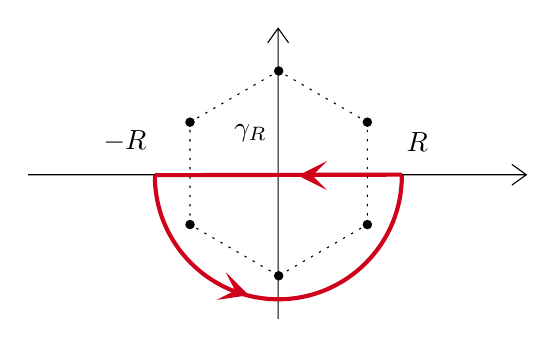
\begin{tikzpicture}[x=0.75pt,y=0.75pt,yscale=-1,xscale=1]
%uncomment if require: \path (0,160); %set diagram left start at 0, and has height of 160

%Shape: Axis 2D [id:dp508857242987794] 
\draw  (170,80) -- (410,80)(290.4,9.41) -- (290.4,149.41) (403,75) -- (410,80) -- (403,85) (285.4,16.41) -- (290.4,9.41) -- (295.4,16.41)  ;
%Shape: Arc [id:dp2429361463821933] 
\draw  [draw opacity=0][line width=1.5]  (350,80.14) .. controls (350,80.26) and (350,80.38) .. (350,80.5) .. controls (350,113.36) and (323.36,140) .. (290.5,140) .. controls (257.64,140) and (231,113.36) .. (231,80.5) .. controls (231,80.4) and (231,80.31) .. (231,80.21) -- (290.5,80.5) -- cycle ; \draw  [color={rgb, 255:red, 208; green, 2; blue, 27 }  ,draw opacity=1 ][line width=1.5]  (350,80.14) .. controls (350,80.26) and (350,80.38) .. (350,80.5) .. controls (350,113.36) and (323.36,140) .. (290.5,140) .. controls (257.64,140) and (231,113.36) .. (231,80.5) .. controls (231,80.4) and (231,80.31) .. (231,80.21) ;
%Shape: Circle [id:dp8781397774455211] 
\draw  [fill={rgb, 255:red, 0; green, 0; blue, 0 }  ,fill opacity=1 ] (288.67,30) .. controls (288.67,28.9) and (289.56,28) .. (290.67,28) .. controls (291.77,28) and (292.67,28.9) .. (292.67,30) .. controls (292.67,31.1) and (291.77,32) .. (290.67,32) .. controls (289.56,32) and (288.67,31.1) .. (288.67,30) -- cycle ;
%Shape: Circle [id:dp3148978419514976] 
\draw  [fill={rgb, 255:red, 0; green, 0; blue, 0 }  ,fill opacity=1 ] (331.39,54.67) .. controls (331.39,53.56) and (332.29,52.67) .. (333.39,52.67) .. controls (334.5,52.67) and (335.39,53.56) .. (335.39,54.67) .. controls (335.39,55.77) and (334.5,56.67) .. (333.39,56.67) .. controls (332.29,56.67) and (331.39,55.77) .. (331.39,54.67) -- cycle ;
%Shape: Circle [id:dp8279624449312546] 
\draw  [fill={rgb, 255:red, 0; green, 0; blue, 0 }  ,fill opacity=1 ] (245.94,104) .. controls (245.94,102.9) and (246.84,102) .. (247.94,102) .. controls (249.05,102) and (249.94,102.9) .. (249.94,104) .. controls (249.94,105.1) and (249.05,106) .. (247.94,106) .. controls (246.84,106) and (245.94,105.1) .. (245.94,104) -- cycle ;
%Shape: Circle [id:dp5338705832900976] 
\draw  [fill={rgb, 255:red, 0; green, 0; blue, 0 }  ,fill opacity=1 ] (331.39,104) .. controls (331.39,102.9) and (332.29,102) .. (333.39,102) .. controls (334.5,102) and (335.39,102.9) .. (335.39,104) .. controls (335.39,105.1) and (334.5,106) .. (333.39,106) .. controls (332.29,106) and (331.39,105.1) .. (331.39,104) -- cycle ;
\draw  [draw opacity=0][fill={rgb, 255:red, 208; green, 2; blue, 27 }  ,fill opacity=1 ] (314,87.41) -- (300,80.41) -- (314,73.41) -- (307,80.41) -- cycle ;
%Straight Lines [id:da4843584145229285] 
\draw [color={rgb, 255:red, 208; green, 2; blue, 27 }  ,draw opacity=1 ][line width=1.5]    (231,80.21) -- (349.99,79.95) ;
\draw  [draw opacity=0][fill={rgb, 255:red, 208; green, 2; blue, 27 }  ,fill opacity=1 ] (265.21,126.99) -- (276.31,138.03) -- (260.82,140.28) -- (269.66,135.83) -- cycle ;
%Shape: Regular Polygon [id:dp2801234129072723] 
\draw  [dash pattern={on 0.84pt off 2.51pt}] (290.67,128.67) -- (247.94,104) -- (247.94,54.67) -- (290.67,30) -- (333.39,54.67) -- (333.39,104) -- cycle ;
%Shape: Circle [id:dp21637549294959646] 
\draw  [fill={rgb, 255:red, 0; green, 0; blue, 0 }  ,fill opacity=1 ] (288.67,128.67) .. controls (288.67,127.56) and (289.56,126.67) .. (290.67,126.67) .. controls (291.77,126.67) and (292.67,127.56) .. (292.67,128.67) .. controls (292.67,129.77) and (291.77,130.67) .. (290.67,130.67) .. controls (289.56,130.67) and (288.67,129.77) .. (288.67,128.67) -- cycle ;
%Shape: Circle [id:dp24691945495063838] 
\draw  [fill={rgb, 255:red, 0; green, 0; blue, 0 }  ,fill opacity=1 ] (245.94,54.67) .. controls (245.94,53.56) and (246.84,52.67) .. (247.94,52.67) .. controls (249.05,52.67) and (249.94,53.56) .. (249.94,54.67) .. controls (249.94,55.77) and (249.05,56.67) .. (247.94,56.67) .. controls (246.84,56.67) and (245.94,55.77) .. (245.94,54.67) -- cycle ;

% Text Node
\draw (268,54.4) node [anchor=north west][inner sep=0.75pt]    {$\gamma _{R}$};
% Text Node
\draw (351,58.4) node [anchor=north west][inner sep=0.75pt]    {$R$};
% Text Node
\draw (205,57.4) node [anchor=north west][inner sep=0.75pt]    {$-R$};


\end{tikzpicture}
\end{figure}
\FloatBarrier

\begin{equation*}
\int _{\mathbb{R}}\frac{e^{-i\lambda x}}{x^{6} +64} dx=-\lim\limits _{R\rightarrow \infty }\int _{\gamma _{R}}\frac{e^{-i\lambda z}}{z^{6} +64} dz=-2\pi i\left[\sum \mathrm{Res}\left( f,z_{k}\right)\right]
\end{equation*}
Gli zeri al denominatore di $f$ sono nelle $6$ radici seste di $-64$ (i vertici di un esagono)
\begin{equation*}
\pm \sqrt{3} \pm i\ \ \ \ \pm 2i
\end{equation*}
Quelli che stanno dentro la parte di piano interessata sono
\begin{equation*}
\pm \sqrt{3} -i\ \ \ \ -2i
\end{equation*}
Per calcolare il residuo in tali punti utilizziamo la formula di calcolo vista anche nel precedente esercizio
\begin{equation*}
\mathrm{Res}\left( f,z_{k}\right) =\left. \frac{e^{-i\lambda z}}{6z^{5}}\right| _{z=z_{k}} =\left. \frac{ze^{-i\lambda z}}{6z^{6}}\right| _{z=z_{k}}
\end{equation*}
Pertanto
\begin{itemize}
\item $\mathrm{Res}\left( f,-\sqrt{3} -i\right) =\frac{\left( -\sqrt{3} -i\right) e^{-i\lambda \left( -\sqrt{3} -i\right)}}{6\cdotp \left( -64\right)}$
\item $\mathrm{Res}\left( f,\sqrt{3} -i\right) =\frac{\left(\sqrt{3} -i\right) e^{-i\lambda \left(\sqrt{3} -i\right)}}{6\cdotp \left( -64\right)}$
\item $\mathrm{Res}\left( f,-2i\right) =\frac{\left( -2i\right) e^{-i\lambda \left( -2i\right)}}{6\cdotp \left( -64\right)}$
\end{itemize}

Allora
\begin{align*}
\int _{\mathbb{R}}\frac{e^{-i\lambda x}}{x^{6} +64} dx & =-2\pi i\left[\frac{\left( -\sqrt{3} -i\right) e^{-i\lambda \left( -\sqrt{3} -i\right)}}{6\cdotp \left( -64\right)} +\frac{\left(\sqrt{3} -i\right) e^{-i\lambda \left(\sqrt{3} -i\right)}}{6\cdotp \left( -64\right)} +\frac{\left( -2i\right) e^{-i\lambda \left( -2i\right)}}{6\cdotp \left( -64\right)}\right]\\
 & =\frac{2\pi i}{6\cdotp 64}\left[\left( -\sqrt{3} -i\right) e^{i\lambda \sqrt{3} -\lambda } +\left(\sqrt{3} -i\right) e^{-i\lambda \sqrt{3} -\lambda } +\left( -2i\right) e^{-2\lambda }\right]\\
 & =\frac{2\pi i}{6\cdotp 64}\left[ -\sqrt{3} e^{i\lambda \sqrt{3} -\lambda } -ie^{i\lambda \sqrt{3} -\lambda } +\sqrt{3} e^{-i\lambda \sqrt{3} -\lambda } -ie^{-i\lambda \sqrt{3} -\lambda } -2ie^{-2\lambda }\right]\\
 & =\frac{2\pi i}{6\cdotp 64}\left[ -\frac{\sqrt{3}}{e^{\lambda }} e^{i\lambda \sqrt{3}} -\frac{i}{e^{\lambda }} e^{i\lambda \sqrt{3}} +\frac{\sqrt{3}}{e^{\lambda }} e^{-i\lambda \sqrt{3}} -\frac{i}{e^{\lambda }} e^{-i\lambda \sqrt{3}} -2ie^{-2\lambda }\right]\\
 & =\frac{2\pi i}{6\cdotp 64\cdotp e^{\lambda }}\left[ -\sqrt{3} e^{i\lambda \sqrt{3}} -ie^{i\lambda \sqrt{3}} +\sqrt{3} e^{-i\lambda \sqrt{3}} -ie^{-i\lambda \sqrt{3}} -2ie^{-\lambda }\right]\\
 & =\frac{2\pi i}{6\cdotp 64\cdotp e^{\lambda }}\left[ -\sqrt{3}\left( e^{i\lambda \sqrt{3}} -e^{-i\lambda \sqrt{3}}\right) -i\left( e^{i\lambda \sqrt{3}} +e^{-i\lambda \sqrt{3}}\right) -2ie^{-\lambda }\right]\\
 & =\frac{2\pi i}{6\cdotp 64\cdotp e^{\lambda }}\left[ -2i\sqrt{3}\frac{\left( e^{i\lambda \sqrt{3}} -e^{-i\lambda \sqrt{3}}\right)}{2i} -2i\frac{\left( e^{i\lambda \sqrt{3}} +e^{-i\lambda \sqrt{3}}\right)}{2} -2ie^{-\lambda }\right]\\
 & =\frac{2\pi i}{6\cdotp 64\cdotp e^{\lambda }}\left[ -2i\sqrt{3}\sin\left( \lambda \sqrt{3}\right) -2i\cos\left( \lambda \sqrt{3}\right) -2ie^{-\lambda }\right]\\
 & =\frac{4\pi }{6\cdotp 64\cdotp e^{\lambda }}\left[\sqrt{3}\sin\left( \lambda \sqrt{3}\right) +\cos\left( \lambda \sqrt{3}\right) +e^{-\lambda }\right]\\
 & =\frac{\pi }{96} e^{-\lambda }\left[\sqrt{3}\sin\left( \lambda \sqrt{3}\right) +\cos\left( \lambda \sqrt{3}\right) +e^{-\lambda }\right]
\end{align*}
Abbiamo appena calcolato la nostra prima trasformata di Fourier. Fare per casa i casi $\lambda =0,\lambda < 0$.
\Soluzione

Questa è un'altra tipologia di integrali, in cui $R$ è una funzione razionale, con seni e coseni, e le loro potenze
\begin{equation*}
\int ^{2\pi }_{0} R\left(\cos \vartheta ,\sin \vartheta \right) d\vartheta 
\end{equation*}
li facciamo per \textit{sostituzione}
\begin{equation*}
\boxed{e^{i\vartheta } =z} \ \ \Rightarrow \ \ \boxed{\cos \vartheta =\frac{z+\frac{1}{z}}{2}} \ \boxed{\sin \vartheta =\frac{z-\frac{1}{z}}{2i}}
\end{equation*}
mentre per il differenziale
\begin{equation*}
ie^{i\vartheta } d\vartheta =dz\ \ \Rightarrow \ \ \boxed{d\vartheta =\frac{1}{iz} dz}
\end{equation*}
Veniamo ora al nostro integrale
\begin{equation*}
\int ^{\pi }_{0}\frac{1}{a+b\cos \vartheta } d\vartheta =\left\{\text{funzione pari}\right\} =\frac{1}{2}\int ^{2\pi }_{0}\frac{1}{a+b\cos \vartheta } d\vartheta 
\end{equation*}
Riscriviamo il coseno in modo più comodo
\begin{equation*}
\cos \vartheta =\frac{z+\frac{1}{z}}{2} =\frac{z^{2} +1}{2z}
\end{equation*}
allora
\begin{equation*}
\frac{1}{2}\int ^{2\pi }_{0}\frac{1}{a+b\cos \vartheta } d\vartheta =\frac{1}{2}\int _{\left| z\right| =1}\frac{1}{a+b\frac{z^{2} +1}{2z}} \cdotp \frac{1}{iz} dz=\frac{1}{i}\int _{\left| z\right| =1}\frac{1}{bz^{2} +2az+b} dz
\end{equation*}
calcoliamo le radici del denominatore
\begin{equation*}
z=\frac{-a\pm \sqrt{a^{2} -b^{2}}}{b}
\end{equation*}
la radice col $+$ è interna alla circonferenza, quella con il meno sta a sinistra di $-1$ invece, di conseguenza prendiamo
\begin{equation*}
\overline{z} =\frac{-a+\sqrt{a^{2} -b^{2}}}{b}
\end{equation*}
allora
\begin{equation*}
\frac{1}{i}\int _{\left| z\right| =1}\frac{1}{bz^{2} +2az+b} dz=\frac{1}{i} \cdotp 2\pi i\cdotp \mathrm{Res}\left( f,\overline{z}\right) =2\pi \cdotp \mathrm{Res}\left( f,\overline{z}\right)
\end{equation*}
il residuo vale
\begin{equation*}
\mathrm{Res}\left( f,\overline{z}\right) =\left. \frac{1}{2bz+2a}\right| _{z=\overline{z}} =\frac{1}{2\sqrt{a^{2} -b^{2}}}
\end{equation*}
sostituiamo nel nostro integrale
\begin{equation*}
2\pi \cdotp \mathrm{Res}\left( f,\overline{z}\right) =\cancel{2} \pi \cdotp \frac{1}{\cancel{2}\sqrt{a^{2} -b^{2}}} =\frac{\pi }{\sqrt{a^{2} -b^{2}}}
\end{equation*}
abbiamo calcolato un integrale facendo una derivata!
\Soluzione

Per il criterio del confronto asintotico, per $x\rightarrow +\infty $
\begin{equation*}
\frac{e^{\alpha x}}{1+e^{x}} \sim \frac{e^{\alpha x}}{e^{x}} =e^{\left( \alpha -1\right) x}
\end{equation*}
converge per $\left( \alpha -1\right) < 0$, cioè $\alpha < 1$. Mentre per $x\rightarrow -\infty $
\begin{equation*}
\frac{e^{\alpha x}}{1+e^{x}} \sim \frac{e^{\alpha x}}{1} =e^{\alpha x}
\end{equation*}
converge per $\alpha  >0$. Quindi complessivamente converge per $0< \alpha < 1$.

Calcoliamo
\begin{equation*}
\int _{\gamma _{R}} f\left( z\right) dz\ \ \ \ f\left( z\right) =\frac{e^{\alpha z}}{1+e^{z}}
\end{equation*}
Non possiamo usare il lemma di Jordan e ci ricordiamo che $e^{z}$ è periodica
\begin{equation*}
e^{z} =e^{z} \cdotp 1=e^{z} \cdotp e^{2\pi i} =e^{z+2\pi i}
\end{equation*}
la nostra funzione ha quindi singolarità in
\begin{equation*}
e^{z} =-1\ \ \Rightarrow \ \ z=i\left( \pi +2k\pi \right)
\end{equation*}
infinite lungo l'asse immaginaria. Non ha senso prendere una semicirconferenza perché dovremmo inglobare nuovi residui man mano che aumentiamo $R$. Invece prendiamo un rettangolo.


\begin{figure}[htpb]
	\centering
\tikzset{every picture/.style={line width=0.75pt}} %set default line width to 0.75pt        

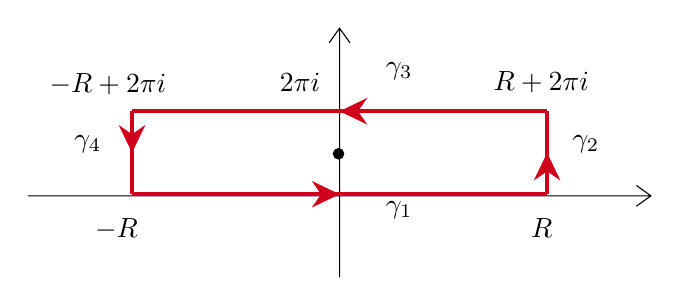
\begin{tikzpicture}[x=0.75pt,y=0.75pt,yscale=-1,xscale=1]
%uncomment if require: \path (0,160); %set diagram left start at 0, and has height of 160

%Shape: Axis 2D [id:dp6952694616964656] 
\draw  (150,110.75) -- (450,110.75)(300,30) -- (300,150) (443,105.75) -- (450,110.75) -- (443,115.75) (295,37) -- (300,30) -- (305,37)  ;
%Shape: Circle [id:dp010000296023957134] 
\draw  [fill={rgb, 255:red, 0; green, 0; blue, 0 }  ,fill opacity=1 ] (297,90.5) .. controls (297,89.12) and (298.12,88) .. (299.5,88) .. controls (300.88,88) and (302,89.12) .. (302,90.5) .. controls (302,91.88) and (300.88,93) .. (299.5,93) .. controls (298.12,93) and (297,91.88) .. (297,90.5) -- cycle ;
%Straight Lines [id:da3282163126700619] 
\draw [color={rgb, 255:red, 208; green, 2; blue, 27 }  ,draw opacity=1 ][line width=1.5]    (200,70) -- (200,110) ;
\draw [shift={(200,90)}, rotate = 270] [fill={rgb, 255:red, 208; green, 2; blue, 27 }  ,fill opacity=1 ][line width=0.08]  [draw opacity=0] (13.4,-6.43) -- (0,0) -- (13.4,6.44) -- (8.9,0) -- cycle    ;
%Straight Lines [id:da8194840593110315] 
\draw [color={rgb, 255:red, 208; green, 2; blue, 27 }  ,draw opacity=1 ][line width=1.5]    (400,110) -- (400,70) ;
\draw [shift={(400,90)}, rotate = 450] [fill={rgb, 255:red, 208; green, 2; blue, 27 }  ,fill opacity=1 ][line width=0.08]  [draw opacity=0] (13.4,-6.43) -- (0,0) -- (13.4,6.44) -- (8.9,0) -- cycle    ;
%Straight Lines [id:da32015283387712334] 
\draw [color={rgb, 255:red, 208; green, 2; blue, 27 }  ,draw opacity=1 ][line width=1.5]    (400,70) -- (200,70) ;
\draw [shift={(300,70)}, rotate = 360] [fill={rgb, 255:red, 208; green, 2; blue, 27 }  ,fill opacity=1 ][line width=0.08]  [draw opacity=0] (13.4,-6.43) -- (0,0) -- (13.4,6.44) -- (8.9,0) -- cycle    ;
%Straight Lines [id:da18099188002221434] 
\draw [color={rgb, 255:red, 208; green, 2; blue, 27 }  ,draw opacity=1 ][line width=1.5]    (200,110) -- (400,110) ;
\draw [shift={(300,110)}, rotate = 180] [fill={rgb, 255:red, 208; green, 2; blue, 27 }  ,fill opacity=1 ][line width=0.08]  [draw opacity=0] (13.4,-6.43) -- (0,0) -- (13.4,6.44) -- (8.9,0) -- cycle    ;

% Text Node
\draw (391,120.4) node [anchor=north west][inner sep=0.75pt]    {$R$};
% Text Node
\draw (181,120.4) node [anchor=north west][inner sep=0.75pt]    {$-R$};
% Text Node
\draw (373,49.4) node [anchor=north west][inner sep=0.75pt]    {$R+2\pi i$};
% Text Node
\draw (159,50.4) node [anchor=north west][inner sep=0.75pt]    {$-R+2\pi i$};
% Text Node
\draw (270,50.4) node [anchor=north west][inner sep=0.75pt]    {$2\pi i$};
% Text Node
\draw (321,112.4) node [anchor=north west][inner sep=0.75pt]    {$\gamma _{1}$};
% Text Node
\draw (411,80.4) node [anchor=north west][inner sep=0.75pt]    {$\gamma _{2}$};
% Text Node
\draw (321,45.4) node [anchor=north west][inner sep=0.75pt]    {$\gamma _{3}$};
% Text Node
\draw (171,80.4) node [anchor=north west][inner sep=0.75pt]    {$\gamma _{4}$};


\end{tikzpicture}
\end{figure}
\FloatBarrier

\begin{equation*}
\int _{\gamma _{R}} f\left( z\right) dz=2\pi i\left[\mathrm{Res}\left( f,\pi i\right)\right] =2\pi i\left[\frac{e^{\alpha z}}{e^{z}}\right]_{z=\pi i} =-2\pi ie^{i\alpha \pi }
\end{equation*}
Vediamo quanto valgono i vari integrali. Quello su $\gamma _{2}$ (e analogamente su $\gamma _{4}$)
\begin{align*}
\left| \int _{\gamma _{2}} f\left( z\right) dz\right|  & =\left\{\gamma _{2} :x=R,y\in \left[ 0,2\pi \right] ,dz=idy\right\} =\\
 & =\left| \int ^{2\pi }_{0}\frac{e^{\alpha R+i\alpha y}}{1+e^{R+iy}} idy\right| \leqslant \int ^{2\pi }_{0}\frac{e^{\alpha R}}{e^{R} -1} dy=2\pi \frac{e^{\alpha R}}{e^{R} -1}\xrightarrow{R\rightarrow +\infty } 0
\end{align*}
Quello su $\gamma _{3}$
\begin{align*}
\int _{\gamma _{3}} f\left( z\right) dz & =\left\{z=x+2\pi i\right\} =\\
 & =-\int ^{R}_{-R}\frac{e^{\alpha x} e^{i2\pi \alpha }}{1+e^{x+2\pi i}} dx=-e^{i2\pi \alpha }\int ^{R}_{-R} f\left( x\right) dx
\end{align*}
quindi
\begin{align*}
\int _{\gamma _{R}} f\left( z\right) dz & \rightarrow -2\pi ie^{i\alpha \pi }\\
\int ^{R}_{-R} f\left( x\right) dx-e^{i2\pi \alpha }\int ^{R}_{-R} f\left( x\right) dx+\underbrace{\int _{\gamma _{2}} f\left( z\right) dz+\int _{\gamma _{4}} f\left( z\right) dz}_{\rightarrow 0} & \rightarrow -2\pi ie^{i\alpha \pi }\\
\left( 1-e^{i2\pi \alpha }\right)\int ^{R}_{-R} f\left( x\right) dx & \rightarrow -2\pi ie^{i\alpha \pi }
\end{align*}
in conclusione
\begin{equation*}
\int _{\mathbb{R}} f\left( x\right) dx=\frac{2\pi ie^{i\alpha \pi }}{e^{i2\pi \alpha } -1} =2\pi i\frac{e^{i\alpha \pi }}{e^{2i\alpha \pi } -1} \cdotp \frac{e^{-i\alpha \pi }}{e^{-i\alpha \pi }} =2\pi i\frac{1}{e^{i\alpha \pi } -e^{-i\alpha \pi }} =\frac{\pi }{\sin\left( \alpha \pi \right)}
\end{equation*}
\chapter{Esercitazione 3 - Potrich}
\ParteEsercizi
\Esercizio{}

Calcolare, al variare di $R >0$
\begin{equation*}
I_{R} =\int _{\gamma _{R}}\frac{\left( z+1\right) e^{\pi z}}{z^{2}\left( z^{2} +1\right)} dz
\end{equation*}
dove
\begin{equation*}
\gamma _{R} :\left| z-1-i\right| =R
\end{equation*}
percorsa positivamente.
\Esercizio{}

Vediamo alcuni integrali reali con metodi di analisi complessa.
\begin{equation*}
I=\boxed{\int ^{2\pi }_{0} R\left(\cos t,\sin t\right) dt}
\end{equation*}
dove $R$ si intende una funzione razionale.
\begin{equation*}
I=\left\{\begin{array}{ c c }
z=e^{it} & \cos t=\frac{e^{it} +e^{-it}}{2}\\
dz=ie^{it} dt & \sin t=\frac{e^{it} -e^{-it}}{2i}
\end{array}\right\} =\int _{\left| z\right| =1} R\left(\frac{z+z^{-1}}{2} ,\frac{z-z^{-1}}{2i}\right)\frac{1}{iz} dz
\end{equation*}
Calcolare
\begin{equation*}
\int ^{2\pi }_{0}\frac{1}{3+\sin t} dt
\end{equation*}
\Esercizio{}

Vediamo una seconda tipologia di integrali
\begin{equation*}
\boxed{\int ^{+\infty }_{-\infty } R\left( x\right) dx} \ \ \ \text{oppure} \ \ \ \ \boxed{\int ^{+\infty }_{-\infty } R\left( x\right)\left\{\begin{array}{ c }
e^{ix}\\
\cos x\\
\sin x
\end{array}\right\} dx}
\end{equation*}
Per risolverli basta porre $f\left( z\right) =R\left( z\right)$ oppure $f\left( z\right) =R\left( z\right) e^{iz}$ e si integra sui semicerchi, infine si fa tendere $R\rightarrow +\infty $.

Se ci fossero poli sull'asse reale devo fare dei morsi e applicare il seguente Lemma. Si fa quindi tendere $\varepsilon \rightarrow 0^{+}$ e $R\rightarrow +\infty $.
\begin{theorem}
[Lemma del cerchio piccolo] Sia $f\in \mathcal{H}\left( D\left( z_{0} ,r\right) \setminus \left\{z_{0}\right\}\right)$, sia $z_{0}$ un polo semplice per $f$, sia $\varphi _{\varepsilon }\left( t\right) =z_{0} +\varepsilon e^{it}$ con $t\in \left[ \alpha ,\beta \right]$. Allora
\begin{equation*}
\lim _{\varepsilon \rightarrow 0^{+}}\int _{\varphi _{\varepsilon }} f\left( z\right) dz=\left( \beta -\alpha \right) i\cdotp \mathrm{Res}\left( f,z_{0}\right)
\end{equation*}
\end{theorem}
\begin{figure}[htpb]
	\centering
\tikzset{every picture/.style={line width=0.75pt}} %set default line width to 0.75pt        

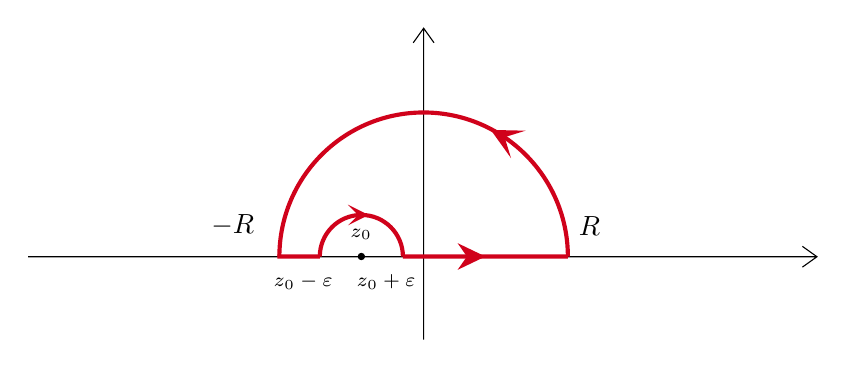
\begin{tikzpicture}[x=0.75pt,y=0.75pt,yscale=-1,xscale=1]
%uncomment if require: \path (0,169); %set diagram left start at 0, and has height of 169

%Shape: Axis 2D [id:dp21276168492453773] 
\draw  (110,120.09) -- (490,120.09)(300.5,10) -- (300.5,160) (483,115.09) -- (490,120.09) -- (483,125.09) (295.5,17) -- (300.5,10) -- (305.5,17)  ;
%Shape: Arc [id:dp9066154861810967] 
\draw  [draw opacity=0][line width=1.5]  (231,120.09) .. controls (231,120.09) and (231,120.09) .. (231,120.09) .. controls (231,81.71) and (262.12,50.59) .. (300.5,50.59) .. controls (338.88,50.59) and (370,81.71) .. (370,120.09) -- (300.5,120.09) -- cycle ; \draw  [color={rgb, 255:red, 208; green, 2; blue, 27 }  ,draw opacity=1 ][line width=1.5]  (231,120.09) .. controls (231,120.09) and (231,120.09) .. (231,120.09) .. controls (231,81.71) and (262.12,50.59) .. (300.5,50.59) .. controls (338.88,50.59) and (370,81.71) .. (370,120.09) ;
%Shape: Arc [id:dp2361543100002761] 
\draw  [draw opacity=0][line width=1.5]  (250.48,119.98) .. controls (250.48,119.98) and (250.48,119.98) .. (250.48,119.98) .. controls (250.48,108.93) and (259.44,99.96) .. (270.5,99.96) .. controls (281.56,99.96) and (290.52,108.93) .. (290.52,119.98) -- (270.5,119.98) -- cycle ; \draw  [color={rgb, 255:red, 208; green, 2; blue, 27 }  ,draw opacity=1 ][line width=1.5]  (250.48,119.98) .. controls (250.48,119.98) and (250.48,119.98) .. (250.48,119.98) .. controls (250.48,108.93) and (259.44,99.96) .. (270.5,99.96) .. controls (281.56,99.96) and (290.52,108.93) .. (290.52,119.98) ;
%Shape: Circle [id:dp06145462056718265] 
\draw  [fill={rgb, 255:red, 0; green, 0; blue, 0 }  ,fill opacity=1 ] (269,119.98) .. controls (269,119.15) and (269.67,118.48) .. (270.5,118.48) .. controls (271.33,118.48) and (272,119.15) .. (272,119.98) .. controls (272,120.81) and (271.33,121.48) .. (270.5,121.48) .. controls (269.67,121.48) and (269,120.81) .. (269,119.98) -- cycle ;
\draw  [draw opacity=0][fill={rgb, 255:red, 208; green, 2; blue, 27 }  ,fill opacity=1 ] (342.64,72.63) -- (332.87,59) -- (349.63,59.36) -- (339.5,62.5) -- cycle ;
%Straight Lines [id:da8537685439706526] 
\draw [color={rgb, 255:red, 208; green, 2; blue, 27 }  ,draw opacity=1 ][line width=1.5]    (230,120) -- (250.48,119.98) ;
%Straight Lines [id:da3820014294051135] 
\draw [color={rgb, 255:red, 208; green, 2; blue, 27 }  ,draw opacity=1 ][line width=1.5]    (290.52,119.98) -- (370,120) ;
\draw [shift={(330.26,119.99)}, rotate = 180.01] [fill={rgb, 255:red, 208; green, 2; blue, 27 }  ,fill opacity=1 ][line width=0.08]  [draw opacity=0] (13.4,-6.43) -- (0,0) -- (13.4,6.44) -- (8.9,0) -- cycle    ;
\draw  [draw opacity=0][fill={rgb, 255:red, 208; green, 2; blue, 27 }  ,fill opacity=1 ] (264,95) -- (274,100) -- (264,105) -- (269,100) -- cycle ;

% Text Node
\draw (197,98.4) node [anchor=north west][inner sep=0.75pt]    {$-R$};
% Text Node
\draw (374,99.4) node [anchor=north west][inner sep=0.75pt]    {$R$};
% Text Node
\draw (227,127.4) node [anchor=north west][inner sep=0.75pt]  [font=\scriptsize]  {$z_{0} -\varepsilon $};
% Text Node
\draw (267,127.4) node [anchor=north west][inner sep=0.75pt]  [font=\scriptsize]  {$z_{0} +\varepsilon $};
% Text Node
\draw (264,105.4) node [anchor=north west][inner sep=0.75pt]  [font=\scriptsize]  {$z_{0}$};


\end{tikzpicture}
\end{figure}
\FloatBarrier
Calcolare
\begin{equation*}
I_{\alpha ,k} =\int ^{+\infty }_{-\infty }\frac{x^{k}}{\alpha ^{2} +x^{2k}} dx\ \ \ \ \alpha  >0,k\in \mathbb{N}
\end{equation*}
\Esercizio{}

Calcolare
\begin{equation*}
I=\int ^{+\infty }_{0}\frac{\sin x}{x} dx
\end{equation*}
\Esercizio{}

Calcolare
\begin{equation*}
\int ^{+\infty }_{-\infty }\frac{\sin\left( \pi x\right)}{\left( x-3\right)\left( x^{2} -2x+2\right)} dx
\end{equation*}
\Esercizio{}

Vediamo una terza tipologia di integrali
\begin{equation*}
\boxed{\int ^{+\infty }_{-\infty } R\left( e^{x}\right)\left\{\begin{array}{ c }
1\\
e^{ix}
\end{array}\right\} dx}
\end{equation*}
Si risolvono integrando sui rettangoli, facendo degli opportuni morsi se e dove necessario.

Calcolare
\begin{equation*}
\int ^{+\infty }_{-\infty }\frac{\cos x}{\cosh x} dx
\end{equation*}
\ParteSoluzioni
\Soluzione

$f\in \mathcal{H}(\mathbb{C} \setminus \{0,\pm i\})$ dove $\pm i$ sono poli semplici, mentre $0$ è un polo del II ordine. 


\begin{figure}[htpb]
	\centering
\tikzset{every picture/.style={line width=0.75pt}} %set default line width to 0.75pt        

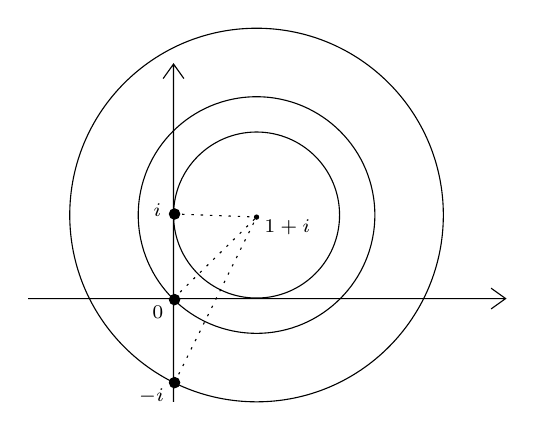
\begin{tikzpicture}[x=0.75pt,y=0.75pt,yscale=-1,xscale=1]
%uncomment if require: \path (0,205); %set diagram left start at 0, and has height of 205

%Shape: Axis 2D [id:dp9998288753339848] 
\draw  (180,140.25) -- (410,140.25)(250,27.25) -- (250,190) (403,135.25) -- (410,140.25) -- (403,145.25) (245,34.25) -- (250,27.25) -- (255,34.25)  ;
%Straight Lines [id:da12445530205724542] 
\draw  [dash pattern={on 0.84pt off 2.51pt}]  (291,101) -- (250.5,99.5) ;
%Shape: Ellipse [id:dp7674970843501638] 
\draw  [fill={rgb, 255:red, 0; green, 0; blue, 0 }  ,fill opacity=1 ] (248,140.75) .. controls (248,139.37) and (249.12,138.25) .. (250.5,138.25) .. controls (251.88,138.25) and (253,139.37) .. (253,140.75) .. controls (253,142.13) and (251.88,143.25) .. (250.5,143.25) .. controls (249.12,143.25) and (248,142.13) .. (248,140.75) -- cycle ;
%Shape: Ellipse [id:dp5063104104492224] 
\draw  [fill={rgb, 255:red, 0; green, 0; blue, 0 }  ,fill opacity=1 ] (248,180.75) .. controls (248,179.37) and (249.12,178.25) .. (250.5,178.25) .. controls (251.88,178.25) and (253,179.37) .. (253,180.75) .. controls (253,182.13) and (251.88,183.25) .. (250.5,183.25) .. controls (249.12,183.25) and (248,182.13) .. (248,180.75) -- cycle ;
%Shape: Ellipse [id:dp3475276859167522] 
\draw  [fill={rgb, 255:red, 0; green, 0; blue, 0 }  ,fill opacity=1 ] (248,99.5) .. controls (248,98.12) and (249.12,97) .. (250.5,97) .. controls (251.88,97) and (253,98.12) .. (253,99.5) .. controls (253,100.88) and (251.88,102) .. (250.5,102) .. controls (249.12,102) and (248,100.88) .. (248,99.5) -- cycle ;
%Shape: Circle [id:dp9945561623234371] 
\draw   (250,100) .. controls (250,77.91) and (267.91,60) .. (290,60) .. controls (312.09,60) and (330,77.91) .. (330,100) .. controls (330,122.09) and (312.09,140) .. (290,140) .. controls (267.91,140) and (250,122.09) .. (250,100) -- cycle ;
%Shape: Circle [id:dp6603014030673247] 
\draw   (233,100) .. controls (233,68.52) and (258.52,43) .. (290,43) .. controls (321.48,43) and (347,68.52) .. (347,100) .. controls (347,131.48) and (321.48,157) .. (290,157) .. controls (258.52,157) and (233,131.48) .. (233,100) -- cycle ;
%Shape: Circle [id:dp8201517506911262] 
\draw   (200,100) .. controls (200,50.29) and (240.29,10) .. (290,10) .. controls (339.71,10) and (380,50.29) .. (380,100) .. controls (380,149.71) and (339.71,190) .. (290,190) .. controls (240.29,190) and (200,149.71) .. (200,100) -- cycle ;
%Shape: Ellipse [id:dp147014916814163] 
\draw  [fill={rgb, 255:red, 0; green, 0; blue, 0 }  ,fill opacity=1 ] (289,101) .. controls (289,100.45) and (289.45,100) .. (290,100) .. controls (290.55,100) and (291,100.45) .. (291,101) .. controls (291,101.55) and (290.55,102) .. (290,102) .. controls (289.45,102) and (289,101.55) .. (289,101) -- cycle ;
%Straight Lines [id:da32148847298984107] 
\draw  [dash pattern={on 0.84pt off 2.51pt}]  (250,140.25) -- (290,101) ;
%Straight Lines [id:da4835195406384667] 
\draw  [dash pattern={on 0.84pt off 2.51pt}]  (250.5,180.75) -- (290,101) ;

% Text Node
\draw (292.5,100.9) node [anchor=north west][inner sep=0.75pt]  [font=\scriptsize]  {$1+i$};
% Text Node
\draw (232,182.4) node [anchor=north west][inner sep=0.75pt]  [font=\scriptsize]  {$-i$};
% Text Node
\draw (238.5,142.4) node [anchor=north west][inner sep=0.75pt]  [font=\scriptsize]  {$0$};
% Text Node
\draw (239,93.4) node [anchor=north west][inner sep=0.75pt]  [font=\scriptsize]  {$i$};


\end{tikzpicture}
\end{figure}
\FloatBarrier

Calcoliamo i residui
\begin{gather*}
\mathrm{Res}\left( f,0\right) =\lim _{z\rightarrow 0}\frac{d}{dz}\left(\left( z-0\right)^{2}\frac{\left( z+1\right) e^{\pi z}}{z^{2}\left( z^{2} +1\right)}\right) =\lim _{z\rightarrow 0}\frac{d}{dz}\frac{\left( z+1\right) e^{\pi z}}{z^{2} +1} =\dotsc =1+\pi \\
\mathrm{Res}\left( f,i\right) =\lim _{z\rightarrow i}\left( z-i\right) f\left( z\right) =\lim _{z\rightarrow i}\frac{\left( z+1\right) e^{\pi z}}{z^{2}\left( z+1\right)} =\dotsc =\frac{1+i}{2i}\\
\mathrm{Res}\left( f,-i\right) =\lim _{z\rightarrow -i}\left( z+i\right) f\left( z\right) =\dotsc =-\frac{1-i}{2i}
\end{gather*}
Le distanze dei punti singolari di $f$ dal centro della curva $\gamma _{R}$ sono
\begin{gather*}
d\left( i,i+1\right) =\left| i-1-i\right| =1\\
d\left( 0,i+1\right) =\left| 1+i\right| =\sqrt{2}\\
d\left( -i,i+1\right) =\left| -i-1-i\right| =\left| -2i-1\right| =\sqrt{5}
\end{gather*}
Allora
\begin{itemize}
\item se $0< R< 1$ per il teorema dei residui\begin{equation*}
I_{R} =0
\end{equation*}
\item se $1< R< \sqrt{2}$ $f$ è olomorfa all'interno di $\gamma _{R}$ tranne che in $z=i$\begin{equation*}
I_{R} =2\pi i\cdotp \mathrm{Res}\left( f,i\right) =\left( 1+i\right) \pi 
\end{equation*}
\item se $\sqrt{2} < R< \sqrt{5}$ $f$ è olomorfa all'interno di $\gamma _{R}$ tranne che in $z=i$ e $z=0$\begin{equation*}
I_{R} =2\pi i\cdotp \left[\mathrm{Res}\left( f,i\right) +\mathrm{Res}\left( f,0\right)\right] =\pi \left( 3\pi +2\pi ^{2}\right) i
\end{equation*}
\item se $R< \sqrt{5}$ tutte le singolarità sono all'interno di $\gamma _{R}$. $f$ è olomorfa all'interno di $\gamma _{R}$ tranne che in $z=\pm i$ e $z=0$\begin{equation*}
I_{R} =2\pi i\cdotp \left[\mathrm{Res}\left( f,0\right) +\mathrm{Res}\left( f,i\right) +\mathrm{Res}\left( f,-i\right)\right]
\end{equation*}
\end{itemize}

Per $R=1,\sqrt{2} ,\sqrt{5}$, $I_{R}$ non può essere calcolato perché $\gamma _{R}$ passa attraverso una singolarità
\Soluzione
\begin{align*}
\int ^{2\pi }_{0}\frac{1}{3+\sin t} dt & =\int _{\left| z\right| =1}\frac{1}{3+\frac{z-z^{-1}}{2i}}\frac{1}{iz} dz\\
 & =\int _{\left| z\right| =1}\frac{2\cancel{iz}}{z^{2} +6iz-1}\frac{1}{\cancel{iz}} dz=2\int _{\left| z\right| =1}\frac{i}{z^{2} +6iz-1} dz
\end{align*}
Le singolarità sono
\begin{equation*}
z^{2} +6iz-1=0\ \ \Leftrightarrow \ \ \begin{cases}
z_{1} =i\left( -3-2\sqrt{2}\right)\\
z_{2} =i\left( -3+2\sqrt{2}\right)
\end{cases}
\end{equation*}
di cui solo $z_{2}$ sta dentro il cerchio unitario
\begin{equation*}
2\int _{\left| z\right| =1}\frac{i}{z^{2} +6iz-1} dz=2\cdotp 2\pi i\cdotp \mathrm{Res}\left( f,i\left( -3+2\sqrt{2}\right)\right)
\end{equation*}
ricordando che è un polo semplice
\begin{equation*}
4\pi i\cdotp \mathrm{Res}\left( f,i\left( -3+2\sqrt{2}\right)\right) =4\pi i\lim\limits _{z\rightarrow i\left( -3+2\sqrt{2}\right)}\left[ z-i\left( -3+2\sqrt{2}\right)\right] f\left( z\right) =\dotsc =\frac{\pi }{\sqrt{2}}
\end{equation*}
\Soluzione
\begin{equation*}
I_{\alpha ,k} =\int ^{+\infty }_{-\infty }\frac{x^{k}}{\alpha ^{2} +x^{2k}} dx\ \ \ \ \alpha  >0,k\in \mathbb{N}
\end{equation*}
Per $x\rightarrow \pm \infty $ si ha $f\left( x\right) \sim \frac{1}{x^{k}}$, che è integrabile in un intorno di $\pm \infty $ se e solo se $k >1$. Quindi $I_{\alpha ,k}$ esiste per $k\in \mathbb{N} ,k\geqslant 2$.

Se $k$ è dispari allora $f$ è dispari e $I_{\alpha ,k} =0$

Se $k$ è pari, con $k\geqslant 2$, poniamo
\begin{equation*}
f\left( z\right) =\frac{z^{k}}{\alpha ^{2} +z^{2k}}
\end{equation*}
Le singolarità si trovano ponendo
\begin{equation*}
z^{2k} =-\alpha ^{2} =\alpha ^{2} e^{\pi i} \ \ \Rightarrow \ \ z_{j} =\alpha ^{\frac{1}{k}} e^{i\frac{\pi +2j\pi }{2k}} \ \ \ \ 0\leqslant j\leqslant k-1
\end{equation*}
allora per il teorema dei residui
\begin{equation*}
\int _{\gamma _{R}} f\left( z\right) dz=\int _{\sigma } f\left( z\right) dz+\int _{\varphi } f\left( z\right) dz=2\pi i\cdotp \sum\limits ^{k-1}_{j=0}\mathrm{Res}\left( f,z_{j}\right)
\end{equation*}
Nello specifico il pezzo su $\sigma $ tende proprio al nostro integrale
\begin{equation*}
\int _{\sigma } f\left( z\right) dz=\left\{z=t,t\in \left[ -R,R\right]\right\} =\int ^{R}_{-R} f\left( t\right) dt\xrightarrow{R\rightarrow +\infty } I_{\alpha ,k}
\end{equation*}
Verifichiamo che
\begin{equation*}
\int _{\varphi } f\left( z\right) dz\rightarrow 0
\end{equation*}
Infatti
\begin{align*}
\left| \int _{\varphi } f\left( z\right) dz\right|  & =\left\{z=Re^{it} ,t\in \left[ 0,\pi \right]\right\} =\left| \int ^{\pi }_{0}\frac{R^{k} e^{ikt}}{\alpha ^{2} +R^{2k} e^{i2kt}} Rie^{it} dt\right| \\
 & \leqslant \int ^{\pi }_{0}\frac{\left| R^{k} e^{ikt}\right| }{\left| \alpha ^{2} +R^{2k} e^{i2kt}\right| }\left| Rie^{it}\right| dt\leqslant \int ^{\pi }_{0}\frac{R^{k+1}}{R^{2k} -\alpha ^{2}} dt\xrightarrow{R\rightarrow +\infty } 0
\end{align*}
dove è stata usata la disuguaglianza triangolare
\begin{nb}
[Disuguaglianza triangolare] Per maggiorazioni e minorazioni ecco la forma più generale della disuguaglianza del triangolo
\begin{equation*}
\left| \left| a\right| -\left| b\right| \right| \leqslant \left| a\pm b\right| \leqslant \left| a\right| +\left| b\right| 
\end{equation*}
\end{nb}

\Soluzione
\begin{equation*}
I=\int ^{+\infty }_{0}\frac{\sin x}{x} dx=\frac{1}{2}\int ^{+\infty }_{-\infty }\frac{\sin x}{x} dx=\frac{1}{2}\mathrm{Im}\left( J\right) \ \ \ \ \ \ \ \ J=\int ^{+\infty }_{-\infty }\frac{e^{ix}}{x} dx
\end{equation*}
Posto $f\left( z\right) =\frac{e^{iz}}{z}$, $f\in \mathcal{H}\left(\mathbb{C} \setminus \left\{0\right\}\right)$. In questo caso devo fare un \textit{morso} in corrispondenza dello $0$.
\begin{equation*}
J=\lim _{\varepsilon \rightarrow 0^{+} ,R\rightarrow +\infty }\int _{\left[ -R,R\right] \setminus \left( -\varepsilon ,\varepsilon \right)}\frac{e^{iz}}{z} dz
\end{equation*}
Per il teorema dell'integrale nullo di Cauchy
\begin{equation*}
0=\int _{\gamma _{R,\varepsilon }} f\left( z\right) dz=\int _{\sigma _{1} \cup \sigma _{2}} f\left( z\right) dz+\int _{\psi } f\left( z\right) dz+\int _{\varphi } f\left( z\right) dz
\end{equation*}
Analizziamo i vari pezzi
\begin{equation*}
\int _{\sigma _{1} \cup \sigma _{2}} f\left( z\right) dz=\left\{z=t,t\in \left[ -R,-\varepsilon \right) \cup \left( \varepsilon ,R\right]\right\} =\int _{\left[ -R,R\right] \setminus \left( -\varepsilon ,\varepsilon \right)}\frac{e^{it}}{t} dt\xrightarrow[\varepsilon \rightarrow 0^{+}]{R\rightarrow +\infty } J
\end{equation*}
il morso:
\begin{equation*}
\int _{\psi } f\left( z\right) dz\xrightarrow{\varepsilon \rightarrow 0^{+}}\left( \beta -\alpha \right) \cdotp \mathrm{Res}\left( f,0\right) =\left( 0-\pi \right) i\cdotp \mathrm{Res}\left( f,0\right) =-\pi i\frac{e^{0}}{1} =-\pi i
\end{equation*}
mentre il semicerchio grande:
\begin{align*}
\left| \int _{\varphi } f\left( z\right) dz\right|  & =\left\{z=Re^{it} ,dz=Rie^{it} dt\right\} =\left| \int ^{\pi }_{0}\frac{e^{iRe^{it}}}{\cancel{Re^{it}}} i\cancel{Re^{it}} dt\right| \\
 & \leqslant \int ^{\pi }_{0}\left| e^{iRe^{it}}\right| dt=\left\{\left| e^{z}\right| =e^{\mathrm{Re}\left( z\right)}\right\}\\
 & =\int ^{\pi }_{0} e^{-R\sin t} dt=2\int ^{\frac{\pi }{2}}_{0} e^{-R\sin t} dt\leqslant 2\int ^{\frac{\pi }{2}}_{0} e^{-\frac{2Rt}{\pi }} dt\\
 & =\frac{\pi }{R}\left( 1-e^{-R}\right) \leqslant \frac{\pi }{R}\xrightarrow{R\rightarrow +\infty } 0
\end{align*}
allora
\begin{equation*}
0=J-\pi i+0\ \ \ \ \Rightarrow \ \ \ \ J=\pi i\ \ \ \ \Rightarrow \ \ \ \ I=\frac{1}{2}\mathrm{Im}\left( J\right) =\frac{\pi }{2}
\end{equation*}
\Soluzione

Dobbiamo calcolare
\begin{equation*}
\int ^{+\infty }_{-\infty }\frac{\sin\left( \pi x\right)}{\left( x-3\right)\left( x^{2} -2x+2\right)} dx
\end{equation*}
poniamo
\begin{equation*}
f\left( z\right) =\frac{e^{i\pi z}}{\left( z-3\right)\left( z^{2} -2z+2\right)}
\end{equation*}
$f\in \mathcal{H}\left(\mathbb{C} \setminus \left\{3,1\pm i\right\}\right)$, uno di essi si trova proprio sulla retta reale, pertanto lì faremo un morso.
\begin{align*}
\int _{\gamma _{R,\varepsilon }} f\left( z\right) dz & =2\pi i\cdotp \mathrm{Res}\left( f,1+i\right) =2\pi i\cdotp \lim _{z\rightarrow 1+i} f\left( z\right)\left( z-\left( 1+i\right)\right) =\\
 & =2\pi i\cdotp \lim _{z\rightarrow 1+i}\frac{e^{\pi iz}}{\left( z-3\right)\left( z-1+i\right)} =\dotsc =\frac{\pi e^{-\pi }}{5}\left( 2+i\right)
\end{align*}
ma questo integrale possiamo vederlo come la somma di tre pezzi
\begin{equation*}
\int _{\gamma _{R,\varepsilon }} f\left( z\right) dz=\int _{\left( -R,3-\varepsilon \right) \cup \left( 3+\varepsilon ,R\right)} f\left( z\right) dz+\int _{\psi } f\left( z\right) dz+\int _{\varphi } f\left( z\right) dz
\end{equation*}
di cui il primo tende proprio all'integrale che vogliamo calcolare
\begin{equation*}
\int _{\left( -R,3-\varepsilon \right) \cup \left( 3+\varepsilon ,R\right)} f\left( z\right) dz\xrightarrow[\varepsilon \rightarrow 0^{+}]{R\rightarrow +\infty }\int ^{+\infty }_{-\infty }\frac{e^{i\pi z}}{\left( x-3\right)\left( x^{2} -2x+2\right)} dx
\end{equation*}
occupiamoci del pezzo sul morso sfruttando il Lemma del cerchio piccolo
\begin{align*}
\lim _{\varepsilon \rightarrow 0^{+}}\int _{\psi } f\left( z\right) dz & =-\pi i\cdotp \mathrm{Res}\left( f,3\right)\\
 & =-\pi i\cdotp \lim _{z\rightarrow 3} f\left( z\right)\left( z-3\right) =-\pi i\cdotp \lim _{z\rightarrow 3}\frac{e^{i\pi z}}{z^{2} -2z+2} =\dotsc =\frac{\pi i}{5}
\end{align*}
ed infine del semicerchio grande
\begin{align*}
\left| \int _{\varphi } f\left( z\right) dz\right|  & =\left\{z=Re^{it} ,dz=Rie^{it} dt\right\}\\
 & =\left| \int ^{\pi }_{0}\frac{e^{\pi iRe^{it}}}{\left( Re^{it} -3\right)\left( R^{2} e^{i2t} -2Re^{it} +2\right)} Rie^{it} dt\right| \\
 & \leqslant \int ^{\pi }_{0}\frac{R}{\left( R-3\right)\left( R^{2} -2R-2\right)} dt=\frac{R\pi }{\left( R-3\right)\left( R^{2} -2R-2\right)}\xrightarrow{R\rightarrow +\infty } 0
\end{align*}
quindi
\begin{equation*}
\int ^{+\infty }_{-\infty }\frac{e^{i\pi x}}{\left( x-3\right)\left( x^{2} -2x+2\right)} dx=-\frac{\pi i}{5} +\frac{\pi e^{-\pi }}{5}\left( 2+i\right)
\end{equation*}
ma l'integrale di partenza è proprio la parte immaginaria di questo integrale
\begin{equation*}
\int ^{+\infty }_{-\infty }\frac{\sin\left( \pi x\right)}{\left( x-3\right)\left( x^{2} -2x+2\right)} dx=\mathrm{Im}\left[ -\frac{\pi i}{5} +\frac{\pi e^{-\pi }}{5}\left( 2+i\right)\right] =\frac{\pi }{5}\left( e^{-\pi } -1\right)
\end{equation*}
\Soluzione

Dobbiamo calcolare
\begin{equation*}
\int ^{+\infty }_{-\infty }\frac{\cos x}{\cosh x} dx
\end{equation*}
consideriamo
\begin{equation*}
f\left( z\right) =\frac{e^{iz}}{\cosh z}
\end{equation*}
il cui denominatore si annulla in
\begin{gather*}
\cosh z=0=\frac{e^{z} +e^{-z}}{2} \ \ \Leftrightarrow \ \ e^{2z} =-1\ \ \Leftrightarrow \ \ 2z=\log\left| -1\right| +i\arg\left( -1\right)\\
\Leftrightarrow \ \ 2z=0+i\left( \pi +2k\pi \right) ,k\in \mathbb{Z} \ \ \Leftrightarrow \ \ z=\frac{\pi i}{2} +k\pi 
\end{gather*}
Integriamo sul rettangolo che contiene il residuo in $\pi i/2$
\begin{equation*}
\int _{\gamma _{R}} f\left( z\right) dz=2\pi i\cdotp \mathrm{Res}\left( f,\frac{\pi i}{2}\right) =2\pi i\cdotp \left. \frac{e^{iz}}{\sinh}\right| _{z=\frac{\pi i}{2}} =\dotsc =\frac{2\pi }{e^{\frac{\pi }{2}}}
\end{equation*}
il circuito lo possiamo vedere come $4$ lati di un rettangolo, numerati in senso antiorario partendo da quello in basso


\begin{figure}[htpb]
	\centering
\tikzset{every picture/.style={line width=0.75pt}} %set default line width to 0.75pt        

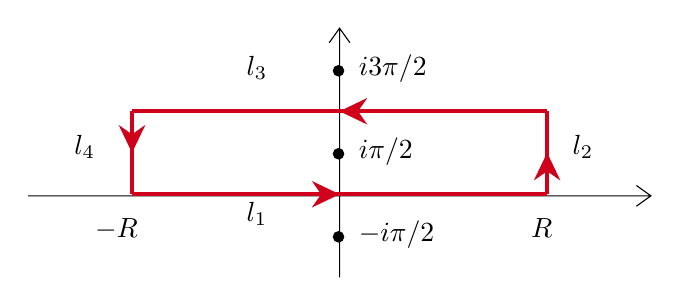
\begin{tikzpicture}[x=0.75pt,y=0.75pt,yscale=-1,xscale=1]
%uncomment if require: \path (0,137); %set diagram left start at 0, and has height of 137

%Shape: Axis 2D [id:dp18751408917716894] 
\draw  (150,90.75) -- (450,90.75)(300,10) -- (300,130) (443,85.75) -- (450,90.75) -- (443,95.75) (295,17) -- (300,10) -- (305,17)  ;
%Shape: Circle [id:dp11440595401764786] 
\draw  [fill={rgb, 255:red, 0; green, 0; blue, 0 }  ,fill opacity=1 ] (297,70.5) .. controls (297,69.12) and (298.12,68) .. (299.5,68) .. controls (300.88,68) and (302,69.12) .. (302,70.5) .. controls (302,71.88) and (300.88,73) .. (299.5,73) .. controls (298.12,73) and (297,71.88) .. (297,70.5) -- cycle ;
%Straight Lines [id:da54907639410711] 
\draw [color={rgb, 255:red, 208; green, 2; blue, 27 }  ,draw opacity=1 ][line width=1.5]    (200,50) -- (200,90) ;
\draw [shift={(200,70)}, rotate = 270] [fill={rgb, 255:red, 208; green, 2; blue, 27 }  ,fill opacity=1 ][line width=0.08]  [draw opacity=0] (13.4,-6.43) -- (0,0) -- (13.4,6.44) -- (8.9,0) -- cycle    ;
%Straight Lines [id:da8839966596936082] 
\draw [color={rgb, 255:red, 208; green, 2; blue, 27 }  ,draw opacity=1 ][line width=1.5]    (400,90) -- (400,50) ;
\draw [shift={(400,70)}, rotate = 450] [fill={rgb, 255:red, 208; green, 2; blue, 27 }  ,fill opacity=1 ][line width=0.08]  [draw opacity=0] (13.4,-6.43) -- (0,0) -- (13.4,6.44) -- (8.9,0) -- cycle    ;
%Straight Lines [id:da5768709170809461] 
\draw [color={rgb, 255:red, 208; green, 2; blue, 27 }  ,draw opacity=1 ][line width=1.5]    (400,50) -- (200,50) ;
\draw [shift={(300,50)}, rotate = 360] [fill={rgb, 255:red, 208; green, 2; blue, 27 }  ,fill opacity=1 ][line width=0.08]  [draw opacity=0] (13.4,-6.43) -- (0,0) -- (13.4,6.44) -- (8.9,0) -- cycle    ;
%Straight Lines [id:da7918111958211875] 
\draw [color={rgb, 255:red, 208; green, 2; blue, 27 }  ,draw opacity=1 ][line width=1.5]    (200,90) -- (400,90) ;
\draw [shift={(300,90)}, rotate = 180] [fill={rgb, 255:red, 208; green, 2; blue, 27 }  ,fill opacity=1 ][line width=0.08]  [draw opacity=0] (13.4,-6.43) -- (0,0) -- (13.4,6.44) -- (8.9,0) -- cycle    ;
%Shape: Circle [id:dp38938153564529987] 
\draw  [fill={rgb, 255:red, 0; green, 0; blue, 0 }  ,fill opacity=1 ] (297,110.5) .. controls (297,109.12) and (298.12,108) .. (299.5,108) .. controls (300.88,108) and (302,109.12) .. (302,110.5) .. controls (302,111.88) and (300.88,113) .. (299.5,113) .. controls (298.12,113) and (297,111.88) .. (297,110.5) -- cycle ;
%Shape: Circle [id:dp5781216178988735] 
\draw  [fill={rgb, 255:red, 0; green, 0; blue, 0 }  ,fill opacity=1 ] (297,30.5) .. controls (297,29.12) and (298.12,28) .. (299.5,28) .. controls (300.88,28) and (302,29.12) .. (302,30.5) .. controls (302,31.88) and (300.88,33) .. (299.5,33) .. controls (298.12,33) and (297,31.88) .. (297,30.5) -- cycle ;

% Text Node
\draw (391,100.4) node [anchor=north west][inner sep=0.75pt]    {$R$};
% Text Node
\draw (181,100.4) node [anchor=north west][inner sep=0.75pt]    {$-R$};
% Text Node
\draw (254,92.4) node [anchor=north west][inner sep=0.75pt]    {$l_{1}$};
% Text Node
\draw (411,60.4) node [anchor=north west][inner sep=0.75pt]    {$l_{2}$};
% Text Node
\draw (254,22.4) node [anchor=north west][inner sep=0.75pt]    {$l_{3}$};
% Text Node
\draw (171,60.4) node [anchor=north west][inner sep=0.75pt]    {$l_{4}$};
% Text Node
\draw (308,61.4) node [anchor=north west][inner sep=0.75pt]    {$i\pi /2$};
% Text Node
\draw (308,101.4) node [anchor=north west][inner sep=0.75pt]    {$-i\pi /2$};
% Text Node
\draw (308,21.4) node [anchor=north west][inner sep=0.75pt]    {$i3\pi /2$};


\end{tikzpicture}
\end{figure}
\FloatBarrier

\begin{equation*}
\int _{\gamma _{R}} f\left( z\right) dz=\int _{l_{1}} f\left( z\right) dz+\int _{l_{2}} f\left( z\right) dz+\int _{l_{3}} f\left( z\right) dz+\int _{l_{4}} f\left( z\right) dz
\end{equation*}
il lato inferiore tende proprio al nostro integrale
\begin{equation*}
\int _{l_{1}} f\left( z\right) dz=\left\{z=t\right\} =\int ^{R}_{-R}\frac{e^{it}}{\cosh t} dt\xrightarrow{R\rightarrow +\infty }\int ^{+\infty }_{-\infty }\frac{e^{it}}{\cosh t} dt
\end{equation*}
mentre il lato superiore tende al nostro integrale moltiplicato per una costante
\begin{align*}
\int _{l_{3}} f\left( z\right) dz & =\left\{z=t+\pi i\right\} =-\int ^{R}_{-R}\frac{e^{i\left( t+\pi i\right)}}{\cosh\left( t+\pi i\right)} dt\\
 & =-\int ^{R}_{-R}\frac{e^{it} e^{-\pi }}{\frac{e^{t+\pi i} +e^{t+\pi i}}{2}} dt=e^{-\pi }\int ^{R}_{-R}\frac{e^{it}}{\cosh t} dt\xrightarrow{R\rightarrow +\infty } e^{-\pi }\int ^{+\infty }_{-\infty }\frac{e^{it}}{\cosh t} dt
\end{align*}
si può dimostrare che i lati verticali tendono a zero
\begin{align*}
\left| \int _{l_{2}} f\left( z\right) dz\right|  & \leqslant \left\{z=R+it,t\in \left[ 0,\pi \right] ,dz=idt\right\} \leqslant \left| \int ^{\pi }_{0}\frac{e^{iR} e^{-t}}{\cosh\left( R+it\right)} idt\right| \\
 & \leqslant \int ^{\pi }_{0}\frac{2e^{-t}}{e^{R} +e^{-R}} dt=\frac{2}{e^{R} +e^{-R}}\int ^{\pi }_{0} e^{-t} dt\xrightarrow{R\rightarrow +\infty } 0
\end{align*}
analogamente
\begin{equation*}
\int _{l_{4}} f\left( z\right) dz\xrightarrow{R\rightarrow +\infty } 0
\end{equation*}
quindi in conclusione
\begin{equation*}
\frac{2\pi }{e^{\frac{\pi }{2}}} =\int ^{+\infty }_{-\infty }\frac{e^{it}}{\cosh t} dt+0+e^{-\pi }\int ^{+\infty }_{-\infty }\frac{e^{it}}{\cosh t} dt+0
\end{equation*}
isoliamo il nostro integrale
\begin{equation*}
\left( 1+e^{-\pi }\right)\int ^{+\infty }_{-\infty }\frac{e^{it}}{\cosh t} d=\frac{2\pi }{e^{\frac{\pi }{2}}} \ \ \Rightarrow \ \ \int ^{+\infty }_{-\infty }\frac{e^{it}}{\cosh t} dt=\frac{2\pi }{\left( 1+e^{-\pi }\right) e^{\frac{\pi }{2}}} =\frac{\pi }{\cosh\left(\frac{\pi }{2}\right)}
\end{equation*}
ma l'integrale di partenza è proprio la parte reale di questo integrale
\begin{equation*}
\int ^{+\infty }_{-\infty }\frac{\cos x}{\cosh x} dx=\mathrm{Re}\left[\int ^{+\infty }_{-\infty }\frac{e^{it}}{\cosh t} dt\right] =\frac{\pi }{\cosh\left(\frac{\pi }{2}\right)}
\end{equation*}
\chapter{Esercitazione 4 - Boella}
\ParteEsercizi
\Esercizio{}

Calcolare il seguente integrale:
\begin{equation*}
\int ^{+\infty }_{0}\frac{\cos (\alpha x)}{x^{2} +\beta ^{2}} dx\ \ \ \ \alpha ,\beta  >0
\end{equation*}
\Esercizio{}

Calcolare il seguente integrale:
\begin{equation*}
\int _{\mathbb{R}}\frac{e^{ix}}{x^{3} +x^{2} +x+1} dx
\end{equation*}
\Esercizio{}

Calcolare l'integrale della funzione polidroma:
\begin{equation*}
\int ^{\infty }_{0}\frac{\sqrt[3]{x}}{x^{2} +4} dx
\end{equation*}
\Esercizio{}

Studiare la convergenza della seguente successione di funzioni:
\begin{equation*}
f_{n} (x)=\frac{\sqrt{n}}{1+(nx)^{2}}
\end{equation*}
\Esercizio{}

Studiare la convergenza della seguente successione di funzioni:
\begin{equation*}
f_{n} (x)=n^{\alpha } \chi _{\left( 0,\frac{1}{n}\right)} (x)
\end{equation*}
\Esercizio{}

Studiare la convergenza della seguente successione di funzioni:
\begin{equation*}
f_{n} (x)=\frac{1-e^{-x}}{x( 1-x)^{1/n}} \chi _{( 0,1)} (x)
\end{equation*}
\ParteSoluzioni
\Soluzione

Ho due vie:
\begin{itemize}
\item Calcolare l'integrale sfruttando le formule di Eulero
\item Farsi furbi (seguiremo questa soluzione)
\end{itemize}

Riconoscendo che la funzione integranda è pari posso scrivere che:
\begin{equation*}
\int ^{+\infty }_{0}\frac{\cos (\alpha x)}{x^{2} +\beta ^{2}} dx\overset{\text{(pari)}}{=}\frac{1}{2}\int _{\mathbb{R}}\frac{\cos (\alpha x)}{x^{2} +\beta ^{2}} dx\overset{\text{(*)}}{=}\frac{1}{2}\left(\int _{\mathbb{R}}\frac{\cos (\alpha x)}{x^{2} +\beta ^{2}} dx+i\int _{\mathbb{R}}\frac{\sin (\alpha x)}{x^{2} +\beta ^{2}} dx\right)
\end{equation*}
Nel passaggio (*) abbiamo sfruttato l'annullamento dell'integrale di una funzione dispari su tutto $\mathbb{R}$. Riconosciamo ora che possiamo riscriverla come:

\begin{equation*}
\frac{1}{2}\int _{\mathbb{R}}\frac{e^{i\alpha x}}{x^{2} +\beta ^{2}} dx
\end{equation*}Prendiamo ora in esame $f(z)=\frac{e^{i\alpha x}}{x^{2} +\beta ^{2}}$, sfruttiamo il Lemma di Jordan ($\alpha  >0$) e il Teorema dei residui, integrando sulla semicirconferenza superiore.
\begin{equation*}
\int _{\gamma _{R}} f( z) dz=2\pi i\cdotp \mathrm{Res}( f,z=i\beta ) =2\pi i\cdotp \left. \frac{e^{i\alpha x}}{2z}\right| _{z=i\beta } =\frac{\pi }{\beta } e^{-\alpha \beta }
\end{equation*}
Per $R\rightarrow +\infty $
\begin{equation*}
\frac{\pi }{\beta } e^{-\alpha \beta } =\int _{\gamma _{R}} =\int ^{R}_{-R} +\cancel{\int _{\sigma _{R}}}\xrightarrow{R\rightarrow +\infty }\int _{\mathbb{R}} f( x) dx\ \ \Rightarrow \ \ \frac{1}{2}\int _{\mathbb{R}}\frac{e^{i\alpha x}}{x^{2} +\beta ^{2}} dx=\frac{\pi e^{-\alpha \beta }}{2\beta }
\end{equation*}
\Soluzione

C'è un asintoto verticale in $x=-1$, quindi non converge.\begin{equation*}
\int _{\mathbb{R}}\frac{e^{ix}}{x^{3} +x^{2} +x+1} dx=\int _{\mathbb{R}}\frac{e^{ix}}{(x^{2} +1)(x+1)} dx
\end{equation*}

Non calcoliamo lui, ma il suo \textit{Valore Principale:} ovvero dobbiamo fare i limiti tutti insieme, non separati. In caso di forme di indecisione $( \infty -\infty )$ potrebbe saltare fuori qualcosa di buono.
\begin{equation*}
( VP)\int _{\mathbb{R}}\frac{e^{ix}}{(x^{2} +1)(x+1)} dx=\lim _{\varepsilon \rightarrow 0^{+} \ R\rightarrow \infty }\left[\int ^{-1-\varepsilon }_{-R} f(x)dx+\int ^{R}_{-1+\varepsilon } f(x)dx\right]
\end{equation*}
Rinfrescate le idee, ora consideriamo come dominio di integrazione una semicirconferenza come raffigurata e scomponiamo l'integrale sulle 4 curve (due tratti curvilinei e due rettilinei, prima e dopo la circonferenza interna).


\begin{figure}[htpb]
	\centering
\tikzset{every picture/.style={line width=0.75pt}} %set default line width to 0.75pt        

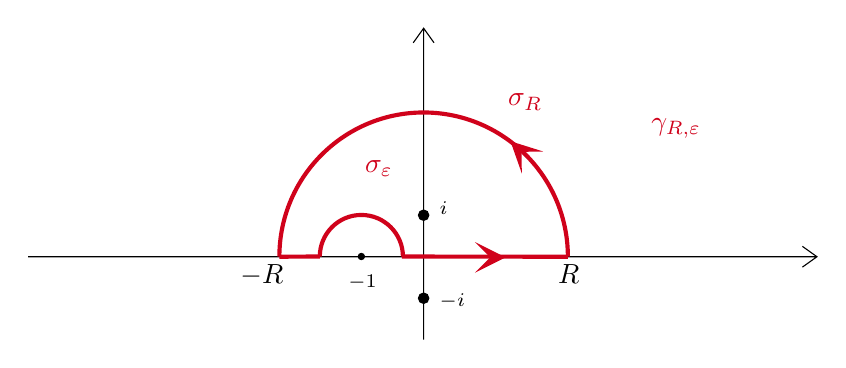
\begin{tikzpicture}[x=0.75pt,y=0.75pt,yscale=-1,xscale=1]
%uncomment if require: \path (0,166); %set diagram left start at 0, and has height of 166

%Shape: Axis 2D [id:dp4597416392621234] 
\draw  (110,120.09) -- (490,120.09)(300.5,10) -- (300.5,160) (483,115.09) -- (490,120.09) -- (483,125.09) (295.5,17) -- (300.5,10) -- (305.5,17)  ;
%Shape: Arc [id:dp48689113730354094] 
\draw  [draw opacity=0][line width=1.5]  (231,120.09) .. controls (231,120.09) and (231,120.09) .. (231,120.09) .. controls (231,81.71) and (262.12,50.59) .. (300.5,50.59) .. controls (338.88,50.59) and (370,81.71) .. (370,120.09) -- (300.5,120.09) -- cycle ; \draw  [color={rgb, 255:red, 208; green, 2; blue, 27 }  ,draw opacity=1 ][line width=1.5]  (231,120.09) .. controls (231,120.09) and (231,120.09) .. (231,120.09) .. controls (231,81.71) and (262.12,50.59) .. (300.5,50.59) .. controls (338.88,50.59) and (370,81.71) .. (370,120.09) ;
%Shape: Arc [id:dp3783656851334405] 
\draw  [draw opacity=0][line width=1.5]  (250.48,119.98) .. controls (250.48,119.98) and (250.48,119.98) .. (250.48,119.98) .. controls (250.48,108.93) and (259.44,99.96) .. (270.5,99.96) .. controls (281.56,99.96) and (290.52,108.93) .. (290.52,119.98) -- (270.5,119.98) -- cycle ; \draw  [color={rgb, 255:red, 208; green, 2; blue, 27 }  ,draw opacity=1 ][line width=1.5]  (250.48,119.98) .. controls (250.48,119.98) and (250.48,119.98) .. (250.48,119.98) .. controls (250.48,108.93) and (259.44,99.96) .. (270.5,99.96) .. controls (281.56,99.96) and (290.52,108.93) .. (290.52,119.98) ;
%Shape: Circle [id:dp8264521136482348] 
\draw  [fill={rgb, 255:red, 0; green, 0; blue, 0 }  ,fill opacity=1 ] (269,119.98) .. controls (269,119.15) and (269.67,118.48) .. (270.5,118.48) .. controls (271.33,118.48) and (272,119.15) .. (272,119.98) .. controls (272,120.81) and (271.33,121.48) .. (270.5,121.48) .. controls (269.67,121.48) and (269,120.81) .. (269,119.98) -- cycle ;
\draw  [draw opacity=0][fill={rgb, 255:red, 208; green, 2; blue, 27 }  ,fill opacity=1 ] (347.82,80) -- (342.34,64.44) -- (358.08,69.39) -- (347.64,69.57) -- cycle ;
\draw  [draw opacity=0][fill={rgb, 255:red, 208; green, 2; blue, 27 }  ,fill opacity=1 ] (325.24,113) -- (340,120.38) -- (325.24,127.76) -- (332.62,120.38) -- cycle ;
%Straight Lines [id:da6476958893771378] 
\draw [color={rgb, 255:red, 208; green, 2; blue, 27 }  ,draw opacity=1 ][line width=1.5]    (231,120.09) -- (250.48,119.98) ;
%Straight Lines [id:da8263168573202715] 
\draw [color={rgb, 255:red, 208; green, 2; blue, 27 }  ,draw opacity=1 ][line width=1.5]    (290,120) -- (370,120.09) ;
%Shape: Circle [id:dp7603714452226784] 
\draw  [fill={rgb, 255:red, 0; green, 0; blue, 0 }  ,fill opacity=1 ] (298,100.09) .. controls (298,98.71) and (299.12,97.59) .. (300.5,97.59) .. controls (301.88,97.59) and (303,98.71) .. (303,100.09) .. controls (303,101.47) and (301.88,102.59) .. (300.5,102.59) .. controls (299.12,102.59) and (298,101.47) .. (298,100.09) -- cycle ;
%Shape: Circle [id:dp46768054307943396] 
\draw  [fill={rgb, 255:red, 0; green, 0; blue, 0 }  ,fill opacity=1 ] (298,140.09) .. controls (298,138.71) and (299.12,137.59) .. (300.5,137.59) .. controls (301.88,137.59) and (303,138.71) .. (303,140.09) .. controls (303,141.47) and (301.88,142.59) .. (300.5,142.59) .. controls (299.12,142.59) and (298,141.47) .. (298,140.09) -- cycle ;

% Text Node
\draw (211,122.4) node [anchor=north west][inner sep=0.75pt]    {$-R$};
% Text Node
\draw (364,122.4) node [anchor=north west][inner sep=0.75pt]    {$R$};
% Text Node
\draw (263,127.4) node [anchor=north west][inner sep=0.75pt]  [font=\scriptsize]  {$-1$};
% Text Node
\draw (409,52.4) node [anchor=north west][inner sep=0.75pt]  [color={rgb, 255:red, 208; green, 2; blue, 27 }  ,opacity=1 ]  {$\gamma _{R,\varepsilon }$};
% Text Node
\draw (271,72.4) node [anchor=north west][inner sep=0.75pt]  [color={rgb, 255:red, 208; green, 2; blue, 27 }  ,opacity=1 ]  {$\sigma _{\varepsilon }$};
% Text Node
\draw (340,40.4) node [anchor=north west][inner sep=0.75pt]  [color={rgb, 255:red, 208; green, 2; blue, 27 }  ,opacity=1 ]  {$\sigma _{R}$};
% Text Node
\draw (307,92.4) node [anchor=north west][inner sep=0.75pt]  [font=\scriptsize]  {$i$};
% Text Node
\draw (307,136.4) node [anchor=north west][inner sep=0.75pt]  [font=\scriptsize]  {$-i$};


\end{tikzpicture}
\end{figure}
\FloatBarrier

\begin{equation*}
\int _{\gamma _{R,\varepsilon }} f(z)dz=2\pi i\cdot \mathrm{Res} (f,z=i)=2\pi i\cdotp \left. \frac{e^{iz}}{3z^{2} +2z+1}\right| _{z=i} =2\pi i\cdotp \frac{e^{-1}}{2i-2}
\end{equation*}
Quando $\varepsilon \rightarrow 0^{+} ,R\rightarrow \infty $
\begin{equation*}
\int _{\gamma _{R,\varepsilon }} =\int ^{-1-\varepsilon }_{-R} +\int _{\sigma _{\varepsilon }} +\int ^{R}_{-1-\varepsilon } +\int _{\sigma _{R}}
\end{equation*}
\begin{theorem}
[Lemma del cerchio piccolo] Sia $f\in \mathcal{H}( D( z_{0} ,r) \setminus \{z_{0}\})$, sia $z_{0}$ un polo semplice per $f$, sia $\varphi _{\varepsilon }( t) =z_{0} +\varepsilon e^{it}$ con $t\in [ \alpha ,\beta ]$. Allora
\begin{equation*}
\lim _{\varepsilon \rightarrow 0^{+}}\int _{\varphi _{\varepsilon }} f( z) dz=( \beta -\alpha ) i\cdotp \mathrm{Res}( f,z_{0})
\end{equation*}
\end{theorem}
Per Jordan, quello su $\sigma _{R}$ tende a $0$.

Per il lemma del cerchio piccolo, quello su $\sigma _{\varepsilon }$ tende a $( 0-\pi ) i\cdotp \mathrm{Res}( f,-1)$.

Applichiamo anche il teorema dei residui sull'integrale su $\gamma _{R,\varepsilon }$.
\begin{equation*}
\begin{aligned}
\int _{\gamma _{R,\varepsilon }} & =\int ^{-1-\varepsilon }_{-R} +\int ^{R}_{-1-\varepsilon } +\int _{\sigma _{\varepsilon }} +\int _{\sigma _{R}}\\
2\pi i\cdotp \mathrm{Res} (f,i) & =\int _{\mathbb{R}} f( x) dx-\pi i\cdotp \mathrm{Res}( f,-1) +0
\end{aligned}
\end{equation*}
Ovvero
\begin{equation*}
\begin{aligned}
\int _{\mathbb{R}} f( x) dx & =2\pi i\cdotp \mathrm{Res} (f,i)+\pi i\cdotp \mathrm{Res}( f,-1)\\
 & =2\pi i\cdotp \frac{e^{-1}}{2i-2} +\pi i\cdotp \frac{e^{-i}}{2}\\
 & =\pi i\left(\frac{e^{-1}}{i-1} +\frac{e^{-i}}{2}\right)
\end{aligned}
\end{equation*}
\Soluzione

Siamo nella seguente situazione


\begin{figure}[htpb]
	\centering
\tikzset{every picture/.style={line width=0.75pt}} %set default line width to 0.75pt        

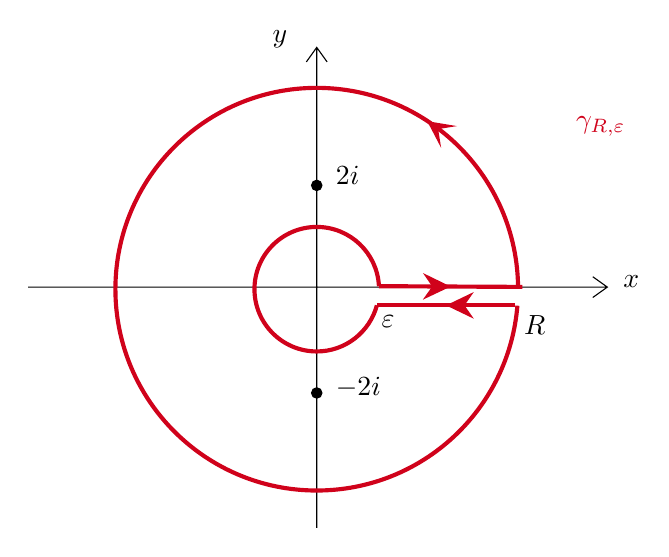
\begin{tikzpicture}[x=0.75pt,y=0.75pt,yscale=-1,xscale=1]
%uncomment if require: \path (0,253); %set diagram left start at 0, and has height of 253

%Shape: Axis 2D [id:dp4998430184566036] 
\draw  (162.5,129.13) -- (441.5,129.13)(301.5,13.63) -- (301.5,245.13) (434.5,124.13) -- (441.5,129.13) -- (434.5,134.13) (296.5,20.63) -- (301.5,13.63) -- (306.5,20.63)  ;
%Straight Lines [id:da677349311209462] 
\draw [color={rgb, 255:red, 208; green, 2; blue, 27 }  ,draw opacity=1 ][line width=1.5]    (331.47,128.68) -- (400.59,129.03) ;
\draw [shift={(366.03,128.85)}, rotate = 180.29] [fill={rgb, 255:red, 208; green, 2; blue, 27 }  ,fill opacity=1 ][line width=0.08]  [draw opacity=0] (13.4,-6.43) -- (0,0) -- (13.4,6.44) -- (8.9,0) -- cycle    ;
%Shape: Arc [id:dp05736289743124079] 
\draw  [draw opacity=0][line width=1.5]  (330.48,137.92) .. controls (327.04,150.71) and (315.37,160.13) .. (301.5,160.13) .. controls (284.93,160.13) and (271.5,146.69) .. (271.5,130.13) .. controls (271.5,113.56) and (284.93,100.13) .. (301.5,100.13) .. controls (317.58,100.13) and (330.71,112.78) .. (331.47,128.68) -- (301.5,130.13) -- cycle ; \draw  [color={rgb, 255:red, 208; green, 2; blue, 27 }  ,draw opacity=1 ][line width=1.5]  (330.48,137.92) .. controls (327.04,150.71) and (315.37,160.13) .. (301.5,160.13) .. controls (284.93,160.13) and (271.5,146.69) .. (271.5,130.13) .. controls (271.5,113.56) and (284.93,100.13) .. (301.5,100.13) .. controls (317.58,100.13) and (330.71,112.78) .. (331.47,128.68) ;
%Shape: Arc [id:dp5246954139360556] 
\draw  [draw opacity=0][line width=1.5]  (398.18,138.07) .. controls (394.14,187.93) and (352.4,227.13) .. (301.5,227.13) .. controls (247.93,227.13) and (204.5,183.7) .. (204.5,130.13) .. controls (204.5,76.55) and (247.93,33.13) .. (301.5,33.13) .. controls (354.77,33.13) and (398.01,76.06) .. (398.5,129.21) -- (301.5,130.13) -- cycle ; \draw  [color={rgb, 255:red, 208; green, 2; blue, 27 }  ,draw opacity=1 ][line width=1.5]  (398.18,138.07) .. controls (394.14,187.93) and (352.4,227.13) .. (301.5,227.13) .. controls (247.93,227.13) and (204.5,183.7) .. (204.5,130.13) .. controls (204.5,76.55) and (247.93,33.13) .. (301.5,33.13) .. controls (354.77,33.13) and (398.01,76.06) .. (398.5,129.21) ;
%Straight Lines [id:da5817066561864661] 
\draw [color={rgb, 255:red, 208; green, 2; blue, 27 }  ,draw opacity=1 ][line width=1.5]    (397.11,137.92) -- (330.48,137.92) ;
\draw [shift={(363.79,137.92)}, rotate = 360] [fill={rgb, 255:red, 208; green, 2; blue, 27 }  ,fill opacity=1 ][line width=0.08]  [draw opacity=0] (13.4,-6.43) -- (0,0) -- (13.4,6.44) -- (8.9,0) -- cycle    ;
\draw  [draw opacity=0][fill={rgb, 255:red, 208; green, 2; blue, 27 }  ,fill opacity=1 ] (361.45,62.08) -- (354.73,49.18) -- (369.08,51.55) -- (360,53) -- cycle ;
%Shape: Circle [id:dp17752216243740282] 
\draw  [color={rgb, 255:red, 0; green, 0; blue, 0 }  ,draw opacity=1 ][fill={rgb, 255:red, 0; green, 0; blue, 0 }  ,fill opacity=1 ] (299,80.13) .. controls (299,78.74) and (300.12,77.63) .. (301.5,77.63) .. controls (302.88,77.63) and (304,78.74) .. (304,80.13) .. controls (304,81.51) and (302.88,82.63) .. (301.5,82.63) .. controls (300.12,82.63) and (299,81.51) .. (299,80.13) -- cycle ;
%Shape: Circle [id:dp22166509967433679] 
\draw  [color={rgb, 255:red, 0; green, 0; blue, 0 }  ,draw opacity=1 ][fill={rgb, 255:red, 0; green, 0; blue, 0 }  ,fill opacity=1 ] (299,180.13) .. controls (299,178.74) and (300.12,177.63) .. (301.5,177.63) .. controls (302.88,177.63) and (304,178.74) .. (304,180.13) .. controls (304,181.51) and (302.88,182.63) .. (301.5,182.63) .. controls (300.12,182.63) and (299,181.51) .. (299,180.13) -- cycle ;

% Text Node
\draw (400.18,141.47) node [anchor=north west][inner sep=0.75pt]    {$R$};
% Text Node
\draw (448,122.4) node [anchor=north west][inner sep=0.75pt]    {$x$};
% Text Node
\draw (279,4.4) node [anchor=north west][inner sep=0.75pt]    {$y$};
% Text Node
\draw (331.48,141.52) node [anchor=north west][inner sep=0.75pt]    {$\varepsilon $};
% Text Node
\draw (425.18,45.47) node [anchor=north west][inner sep=0.75pt]  [color={rgb, 255:red, 208; green, 2; blue, 27 }  ,opacity=1 ]  {$\gamma _{R,\varepsilon }$};
% Text Node
\draw (309.48,69.52) node [anchor=north west][inner sep=0.75pt]    {$2i$};
% Text Node
\draw (309.48,171.52) node [anchor=north west][inner sep=0.75pt]    {$-2i$};


\end{tikzpicture}
\end{figure}
\FloatBarrier

Se prendiamo
\begin{equation*}
f( z) =\frac{\sqrt[3]{z}}{z^{2} +4}
\end{equation*}
abbiamo diversi problemi. Dobbiamo assicurarci di prendere la determinazione reale della radice.
\begin{equation*}
f(\rho ,\vartheta )=\frac{\sqrt[3]{\rho } e^{i\vartheta /3}}{\rho ^{2} e^{2i\vartheta } +4}
\end{equation*}
I poli sono in $\pm 2i$
\begin{equation*}
\begin{aligned}
\int _{\gamma _{R,\varepsilon }} f( z) dz & =2\pi i\cdotp \left(\frac{\sqrt[3]{2} e^{i\frac{\pi }{2} /3}}{4i} +\frac{\sqrt[3]{2} e^{i\frac{3\pi }{2} /3}}{-4i}\right) =\frac{\pi \sqrt[3]{2}}{2}\left( e^{i\frac{\pi }{6}} -e^{i\frac{\pi }{2}}\right)\\
\int _{\gamma _{R,\varepsilon }} f( z) dz & =\int ^{R}_{\varepsilon } +\int _{\sigma _{R}} +\int ^{\varepsilon }_{R} +\int _{\sigma _{\varepsilon }}
\end{aligned}
\end{equation*}
I due integrali sulle circonferenze tendono a $0$, con opportune maggiorazioni.

L'integrale che ci interessa è
\begin{equation*}
\int ^{R}_{\varepsilon } f( z) dz=\int ^{R}_{\varepsilon }\frac{\sqrt[3]{\rho }}{\rho ^{2} +4} d\rho \rightarrow I
\end{equation*}
L'integrale contromano va fatto facendo \textbf{attenzione} che $\vartheta =2\pi $, non più zero.
\begin{equation*}
\int ^{\varepsilon }_{R} f( z) dz=-\int ^{R}_{\varepsilon } f( z) dz=-\int ^{R}_{\varepsilon }\frac{\sqrt[3]{\rho } e^{i2\pi /3}}{\rho ^{2} +4} d\rho \rightarrow -Ie^{i2\pi /3}
\end{equation*}
Allora deduciamo che
\begin{equation*}
\begin{aligned}
\int _{\gamma _{R,\varepsilon }} & =\int ^{R}_{\varepsilon } +\int _{\sigma _{R}} +\int ^{\varepsilon }_{R} +\int _{\sigma _{\varepsilon }}\\
\frac{\pi \sqrt[3]{2}}{2}\left( e^{i\frac{\pi }{6}} -e^{i\frac{\pi }{2}}\right) & =I+0-Ie^{i2\pi /3} +0\\
 & \Rightarrow \ \ I=\frac{\frac{\pi \sqrt[3]{2}}{2}\left( e^{i\frac{\pi }{6}} -e^{i\frac{\pi }{2}}\right)}{1-e^{i2\pi /3}}
\end{aligned}
\end{equation*}
Che possiamo riscrivere
\begin{equation*}
I=\frac{\frac{\pi \sqrt[3]{2}}{2}\left(\frac{\sqrt{3}}{2} +\frac{1}{2} i-i\right)}{1-\left( -\frac{1}{2} +\frac{\sqrt{3}}{2} i\right)} =\frac{\frac{\pi \sqrt[3]{2}}{2}\left(\frac{\sqrt{3}}{2} -\frac{1}{2} i\right)}{\frac{3}{2} -\frac{\sqrt{3}}{2} i} =\frac{\frac{\pi \sqrt[3]{2}}{2}\left(\frac{\sqrt{3}}{2} -\frac{1}{2} i\right)}{\sqrt{3}\left(\frac{\sqrt{3}}{2} -\frac{1}{2} i\right)} =\frac{\pi \sqrt[3]{2}}{2\sqrt{3}}
\end{equation*}
\Soluzione

Vediamo il grafico

\fg{0.7}{07-4}

Calcoliamo il limite puntuale
\begin{equation*}
f_{n} (x)=\frac{\sqrt{n}}{1+(nx)^{2}}\xrightarrow{n\rightarrow \infty } F(x)=\begin{cases}
+\infty , & x=0\\
0, & x\neq 0
\end{cases} \ \ \Rightarrow \ \ f_{n}\xrightarrow[\text{q.o.}]{n\rightarrow \infty } 0
\end{equation*}
Controlliamo la convergenza in $L^{1}$
\begin{equation*}
\Vert f_{n} -F\Vert _{L^{1}} =\int _{\mathbb{R}}\frac{\sqrt{n}}{1+(nx)^{2}} dx=\left\{\begin{array}{ c }
nx=t\\
dx=\frac{1}{n} dt
\end{array}\right\} =\frac{1}{\sqrt{n}}\int _{\mathbb{R}}\frac{1}{1+t^{2}} dt\xrightarrow{n\rightarrow \infty } 0
\end{equation*}
Controlliamo la convergenza in $L^{p}$:
\begin{gather*}
\Vert f_{n} -F\Vert ^{p}_{L^{p}} =\int _{\mathbb{R}}\frac{n^{p/2}}{(1+(nx)^{2} )^{p}} =\left\{\begin{array}{ c }
nx=t\\
dx=\frac{1}{n} dt
\end{array}\right\} =n^{\frac{p}{2} -1}\int _{\mathbb{R}}\frac{1}{(1+t^{2} )^{p}} dt\\
\\
\Rightarrow \ \ \Vert f_{n} -F\Vert ^{p}_{L^{p}}\xrightarrow{n\rightarrow \infty } 0\ \ \Leftrightarrow \ \ \frac{p}{2} -1< 0\ \ \Leftrightarrow \ \ p< 2
\end{gather*}
Non converge in $L^{\infty }$ perché in $0$ non sono limitate.
\Soluzione

Si può vedere che con $\alpha =2$

\fg{0.6}{07-5}
\begin{equation*}
f_{n} (x)=n^{\alpha } \chi _{\left( 0;\frac{1}{n}\right)} (x)\xrightarrow[\text{q.o}]{n\rightarrow \infty } F(x)\equiv 0
\end{equation*}
Non converge in $L^{\infty }$ perché non sono limitate.

Studiamo la convergenza in $L^{p}$:
\begin{equation*}
\Vert f_{n} -F\Vert ^{p}_{L^{p}} =\int ^{1/n}_{0} n^{\alpha p} dx=n^{\alpha p-1}\rightarrow 0\ \ \Leftrightarrow \ \ \alpha p< 1\ \ \Leftrightarrow \ \ \alpha < \frac{1}{p}
\end{equation*}
\Soluzione

Vediamo il grafico

\fg{0.6}{07-6}

Limite puntuale
\begin{equation*}
\lim\limits _{n\rightarrow +\infty } f_{n}( x) =\frac{1-e^{-x}}{x} \chi _{( 0,1)} (x)=F( x)
\end{equation*}
Non abbiamo problemi di integrabilità in $0$ perché
\begin{equation*}
x\rightarrow 0,\ \ f_{n}( x) \sim \frac{x}{x} =1
\end{equation*}
Mentre in $1$
\begin{equation*}
x\rightarrow 1,\ \ f_{n}( x) \sim \frac{1-e^{-1}}{( 1-x)^{1/n}} \in L^{1}( 0,1) \ \ \Leftrightarrow \ \ n\geqslant 2
\end{equation*}
Quindi
\begin{equation*}
\Vert f_{n} -F\Vert _{L^{1}} =\int ^{1}_{0}\left| \frac{1-e^{-x}}{x( 1-x)^{1/n}} -\frac{1-e^{-x}}{x}\right| dx=\int ^{1}_{0}\frac{1-e^{-x}}{x}\left(\frac{1}{( 1-x)^{1/n}} -1\right) dx
\end{equation*}
Usiamo la convergenza dominata
\begin{equation*}
g_{n}( x) =\frac{1-e^{-x}}{x}\left(\frac{1}{( 1-x)^{1/n}} -1\right)
\end{equation*}
Prendiamo la più grande, $n=2$
\begin{equation*}
| g_{n}( x)| \leqslant g_{2}( x) \in L^{1}
\end{equation*}
Allora possiamo scambiare limite e segno dell'integrale e dedurre che c'è convergenza in $L^{1}$.
\chapter{Esercitazione 4 - Potrich}
\ParteEsercizi
\Esercizio{}

Vediamo una quarta tipologia
\begin{equation*}
\boxed{\int ^{+\infty }_{0} x^{\alpha } R\left( x^{m}\right) dx} \ \ \ \ \alpha \in \mathbb{R} ,m\in \mathbb{N} ,m\geqslant 2
\end{equation*}
Se $\alpha $ è un intero, allora si integra su curve così


\begin{figure}[htpb]
	\centering
\tikzset{every picture/.style={line width=0.75pt}} %set default line width to 0.75pt        

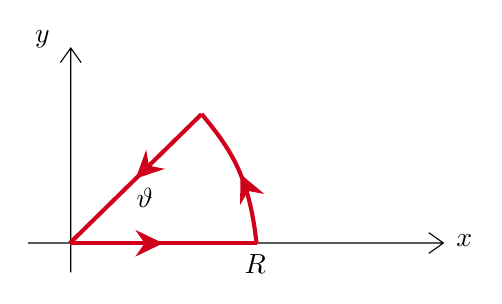
\begin{tikzpicture}[x=0.75pt,y=0.75pt,yscale=-1,xscale=1]
%uncomment if require: \path (0,137); %set diagram left start at 0, and has height of 137

%Shape: Axis 2D [id:dp5724429407600313] 
\draw  (190,109.89) -- (390,109.89)(210.5,15.95) -- (210.5,124) (383,104.89) -- (390,109.89) -- (383,114.89) (205.5,22.95) -- (210.5,15.95) -- (215.5,22.95)  ;
%Straight Lines [id:da6909710830091127] 
\draw [color={rgb, 255:red, 208; green, 2; blue, 27 }  ,draw opacity=1 ][line width=1.5]    (210,110) -- (273.5,47.8) ;
\draw [shift={(241.75,78.9)}, rotate = 315.59] [fill={rgb, 255:red, 208; green, 2; blue, 27 }  ,fill opacity=1 ][line width=0.08]  [draw opacity=0] (13.4,-6.43) -- (0,0) -- (13.4,6.44) -- (8.9,0) -- cycle    ;
%Curve Lines [id:da21980918672783578] 
\draw [color={rgb, 255:red, 208; green, 2; blue, 27 }  ,draw opacity=1 ][line width=1.5]    (273.5,47.69) .. controls (288.5,65.69) and (296.5,78.69) .. (300,110) ;
\draw [shift={(292.32,76.73)}, rotate = 65.41] [fill={rgb, 255:red, 208; green, 2; blue, 27 }  ,fill opacity=1 ][line width=0.08]  [draw opacity=0] (13.4,-6.43) -- (0,0) -- (13.4,6.44) -- (8.9,0) -- cycle    ;
%Straight Lines [id:da9818804804141448] 
\draw [color={rgb, 255:red, 208; green, 2; blue, 27 }  ,draw opacity=1 ][line width=1.5]    (210,110) -- (300,110) ;
\draw [shift={(255,110)}, rotate = 180] [fill={rgb, 255:red, 208; green, 2; blue, 27 }  ,fill opacity=1 ][line width=0.08]  [draw opacity=0] (13.4,-6.43) -- (0,0) -- (13.4,6.44) -- (8.9,0) -- cycle    ;

% Text Node
\draw (293,114.4) node [anchor=north west][inner sep=0.75pt]    {$R$};
% Text Node
\draw (395,104.4) node [anchor=north west][inner sep=0.75pt]    {$x$};
% Text Node
\draw (192,6.4) node [anchor=north west][inner sep=0.75pt]    {$y$};
% Text Node
\draw (241,82.4) node [anchor=north west][inner sep=0.75pt]    {$\vartheta $};


\end{tikzpicture}
\end{figure}
\FloatBarrier

Se $\alpha $ non è un intero, allora si integra su curve così


\begin{figure}[htpb]
	\centering
\tikzset{every picture/.style={line width=0.75pt}} %set default line width to 0.75pt        

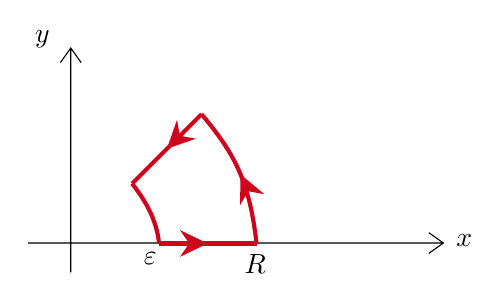
\begin{tikzpicture}[x=0.75pt,y=0.75pt,yscale=-1,xscale=1]
%uncomment if require: \path (0,137); %set diagram left start at 0, and has height of 137

%Shape: Axis 2D [id:dp029235818502451494] 
\draw  (190,109.89) -- (390,109.89)(210.5,15.95) -- (210.5,124) (383,104.89) -- (390,109.89) -- (383,114.89) (205.5,22.95) -- (210.5,15.95) -- (215.5,22.95)  ;
%Straight Lines [id:da5818987952561847] 
\draw [color={rgb, 255:red, 208; green, 2; blue, 27 }  ,draw opacity=1 ][line width=1.5]    (240.05,81.25) -- (273.5,47.8) ;
\draw [shift={(256.77,64.52)}, rotate = 315] [fill={rgb, 255:red, 208; green, 2; blue, 27 }  ,fill opacity=1 ][line width=0.08]  [draw opacity=0] (13.4,-6.43) -- (0,0) -- (13.4,6.44) -- (8.9,0) -- cycle    ;
%Curve Lines [id:da6921320122846151] 
\draw [color={rgb, 255:red, 208; green, 2; blue, 27 }  ,draw opacity=1 ][line width=1.5]    (273.5,47.8) .. controls (288.5,65.8) and (296.5,78.8) .. (300,110.11) ;
\draw [shift={(292.31,76.84)}, rotate = 65.41] [fill={rgb, 255:red, 208; green, 2; blue, 27 }  ,fill opacity=1 ][line width=0.08]  [draw opacity=0] (13.4,-6.43) -- (0,0) -- (13.4,6.44) -- (8.9,0) -- cycle    ;
%Straight Lines [id:da44850949525670036] 
\draw [color={rgb, 255:red, 208; green, 2; blue, 27 }  ,draw opacity=1 ][line width=1.5]    (253,110.11) -- (300,110.11) ;
\draw [shift={(276.5,110.11)}, rotate = 180] [fill={rgb, 255:red, 208; green, 2; blue, 27 }  ,fill opacity=1 ][line width=0.08]  [draw opacity=0] (13.4,-6.43) -- (0,0) -- (13.4,6.44) -- (8.9,0) -- cycle    ;
%Curve Lines [id:da2387592758227124] 
\draw [color={rgb, 255:red, 208; green, 2; blue, 27 }  ,draw opacity=1 ][line width=1.5]    (240.05,81.25) .. controls (245.55,88.25) and (252,98.25) .. (253,110.11) ;

% Text Node
\draw (293,114.4) node [anchor=north west][inner sep=0.75pt]    {$R$};
% Text Node
\draw (395,104.4) node [anchor=north west][inner sep=0.75pt]    {$x$};
% Text Node
\draw (192,6.4) node [anchor=north west][inner sep=0.75pt]    {$y$};
% Text Node
\draw (244.5,113.4) node [anchor=north west][inner sep=0.75pt]    {$\varepsilon $};


\end{tikzpicture}
\end{figure}
\FloatBarrier

L'ampiezza dell'angolo $\vartheta $ deve essere in entrambi i casi $\vartheta =\frac{2\pi }{m}$.



Integriamo la funzione $f( z) =e^{\alpha \log z} R\left( z^{m}\right)$.

\textbf{NB.} Se $m=2$, l'ampiezza dell'angolo sarebbe $2\pi $, tuttavia il dominio del logaritmo esclude che io possa integrare lungo la semiretta $x< 0$.

Se $m=2$ allora tolgo un altro ramo.


\begin{figure}[htpb]
	\centering
\tikzset{every picture/.style={line width=0.75pt}} %set default line width to 0.75pt        

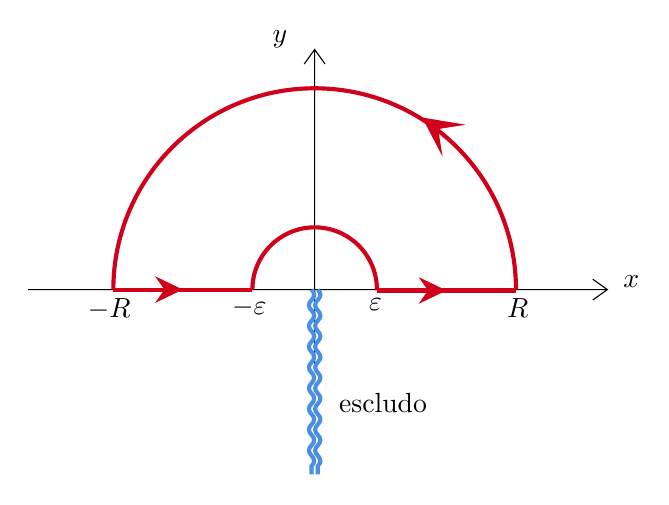
\begin{tikzpicture}[x=0.75pt,y=0.75pt,yscale=-1,xscale=1]
%uncomment if require: \path (0,238); %set diagram left start at 0, and has height of 238

%Shape: Axis 2D [id:dp48898581387364404] 
\draw  (162.5,140.33) -- (441.5,140.33)(300.5,24.63) -- (300.5,179.33) (434.5,135.33) -- (441.5,140.33) -- (434.5,145.33) (295.5,31.63) -- (300.5,24.63) -- (305.5,31.63)  ;
%Straight Lines [id:da5757902151460577] 
\draw [color={rgb, 255:red, 208; green, 2; blue, 27 }  ,draw opacity=1 ][line width=1.5]    (330.5,140.75) -- (397.5,140.75) ;
\draw [shift={(364,140.75)}, rotate = 180] [fill={rgb, 255:red, 208; green, 2; blue, 27 }  ,fill opacity=1 ][line width=0.08]  [draw opacity=0] (13.4,-6.43) -- (0,0) -- (13.4,6.44) -- (8.9,0) -- cycle    ;
%Shape: Arc [id:dp28549627239777453] 
\draw  [draw opacity=0][line width=1.5]  (270.5,140.33) .. controls (270.5,123.76) and (283.93,110.33) .. (300.5,110.33) .. controls (317.07,110.33) and (330.5,123.76) .. (330.5,140.33) .. controls (330.5,140.47) and (330.5,140.61) .. (330.5,140.75) -- (300.5,140.33) -- cycle ; \draw  [color={rgb, 255:red, 208; green, 2; blue, 27 }  ,draw opacity=1 ][line width=1.5]  (270.5,140.33) .. controls (270.5,123.76) and (283.93,110.33) .. (300.5,110.33) .. controls (317.07,110.33) and (330.5,123.76) .. (330.5,140.33) .. controls (330.5,140.47) and (330.5,140.61) .. (330.5,140.75) ;
%Shape: Arc [id:dp39883767783687163] 
\draw  [draw opacity=0][line width=1.5]  (203.5,140.33) .. controls (203.5,86.76) and (246.93,43.33) .. (300.5,43.33) .. controls (354.07,43.33) and (397.5,86.76) .. (397.5,140.33) -- (300.5,140.33) -- cycle ; \draw  [color={rgb, 255:red, 208; green, 2; blue, 27 }  ,draw opacity=1 ][line width=1.5]  (203.5,140.33) .. controls (203.5,86.76) and (246.93,43.33) .. (300.5,43.33) .. controls (354.07,43.33) and (397.5,86.76) .. (397.5,140.33) ;
%Straight Lines [id:da500527919927189] 
\draw [color={rgb, 255:red, 208; green, 2; blue, 27 }  ,draw opacity=1 ][line width=1.5]    (203.5,140.33) -- (270.5,140.33) ;
\draw [shift={(237,140.33)}, rotate = 180] [fill={rgb, 255:red, 208; green, 2; blue, 27 }  ,fill opacity=1 ][line width=0.08]  [draw opacity=0] (13.4,-6.43) -- (0,0) -- (13.4,6.44) -- (8.9,0) -- cycle    ;
\draw  [draw opacity=0][fill={rgb, 255:red, 208; green, 2; blue, 27 }  ,fill opacity=1 ] (362.12,76.27) -- (352.31,57.43) -- (373.27,60.88) -- (360,63) -- cycle ;
%Straight Lines [id:da16629969721545534] 
\draw [color={rgb, 255:red, 74; green, 144; blue, 226 }  ,draw opacity=1 ][line width=1.5]    (302,140.33) .. controls (303.67,142) and (303.67,143.66) .. (302,145.33) .. controls (300.33,147) and (300.33,148.66) .. (302,150.33) .. controls (303.67,152) and (303.67,153.66) .. (302,155.33) .. controls (300.33,157) and (300.33,158.66) .. (302,160.33) .. controls (303.67,162) and (303.67,163.66) .. (302,165.33) .. controls (300.33,167) and (300.33,168.66) .. (302,170.33) .. controls (303.67,172) and (303.67,173.66) .. (302,175.33) .. controls (300.33,177) and (300.33,178.66) .. (302,180.33) .. controls (303.67,182) and (303.67,183.66) .. (302,185.33) .. controls (300.33,187) and (300.33,188.66) .. (302,190.33) .. controls (303.67,192) and (303.67,193.66) .. (302,195.33) .. controls (300.33,197) and (300.33,198.66) .. (302,200.33) .. controls (303.67,202) and (303.67,203.66) .. (302,205.33) .. controls (300.33,207) and (300.33,208.66) .. (302,210.33) .. controls (303.67,212) and (303.67,213.66) .. (302,215.33) .. controls (300.33,217) and (300.33,218.66) .. (302,220.33) .. controls (303.67,222) and (303.67,223.66) .. (302,225.33) -- (302,229.33) -- (302,229.33)(299,140.33) .. controls (300.67,142) and (300.67,143.66) .. (299,145.33) .. controls (297.33,147) and (297.33,148.66) .. (299,150.33) .. controls (300.67,152) and (300.67,153.66) .. (299,155.33) .. controls (297.33,157) and (297.33,158.66) .. (299,160.33) .. controls (300.67,162) and (300.67,163.66) .. (299,165.33) .. controls (297.33,167) and (297.33,168.66) .. (299,170.33) .. controls (300.67,172) and (300.67,173.66) .. (299,175.33) .. controls (297.33,177) and (297.33,178.66) .. (299,180.33) .. controls (300.67,182) and (300.67,183.66) .. (299,185.33) .. controls (297.33,187) and (297.33,188.66) .. (299,190.33) .. controls (300.67,192) and (300.67,193.66) .. (299,195.33) .. controls (297.33,197) and (297.33,198.66) .. (299,200.33) .. controls (300.67,202) and (300.67,203.66) .. (299,205.33) .. controls (297.33,207) and (297.33,208.66) .. (299,210.33) .. controls (300.67,212) and (300.67,213.66) .. (299,215.33) .. controls (297.33,217) and (297.33,218.66) .. (299,220.33) .. controls (300.67,222) and (300.67,223.66) .. (299,225.33) -- (299,229.33) -- (299,229.33) ;

% Text Node
\draw (392,143.4) node [anchor=north west][inner sep=0.75pt]    {$R$};
% Text Node
\draw (448,132.4) node [anchor=north west][inner sep=0.75pt]    {$x$};
% Text Node
\draw (279,14.4) node [anchor=north west][inner sep=0.75pt]    {$y$};
% Text Node
\draw (325.5,143.4) node [anchor=north west][inner sep=0.75pt]    {$\varepsilon $};
% Text Node
\draw (190,143.4) node [anchor=north west][inner sep=0.75pt]    {$-R$};
% Text Node
\draw (259.5,143.4) node [anchor=north west][inner sep=0.75pt]    {$-\varepsilon $};
% Text Node
\draw (311,189) node [anchor=north west][inner sep=0.75pt]   [align=left] {escludo};


\end{tikzpicture}
\end{figure}
\FloatBarrier



Calcolare
\begin{equation*}
I=\int ^{+\infty }_{0}\frac{x^{\alpha }}{1+x^{3}} dx\ \ \ \ \alpha \in \mathbb{R} ,
\end{equation*}
\Esercizio{}

Vediamo una quinta tipologia
\begin{equation*}
\boxed{\begin{array}{ c l }
A & \int ^{+\infty }_{0} x^{\alpha } R( x) dx\ \ \alpha \neq 0\\
B & \int ^{+\infty }_{0} R( x) dx\\
C & \int ^{+\infty }_{0}\ln( x) R( x) dx
\end{array}}
\end{equation*}
Bisogna integrare su


\begin{figure}[htpb]
	\centering
\tikzset{every picture/.style={line width=0.75pt}} %set default line width to 0.75pt        

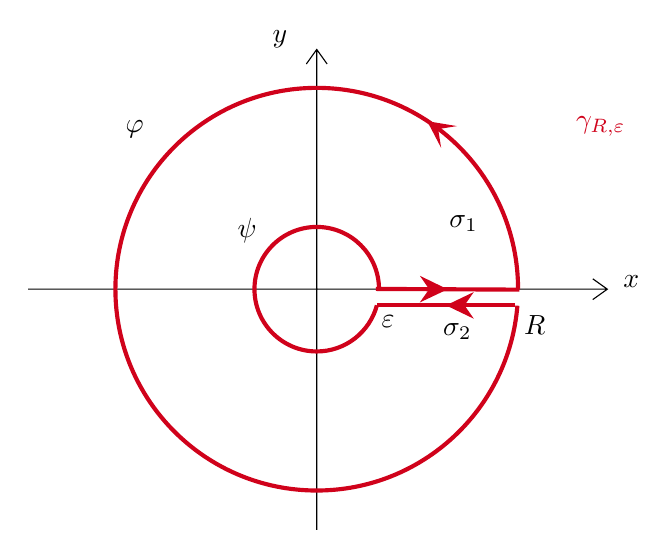
\begin{tikzpicture}[x=0.75pt,y=0.75pt,yscale=-1,xscale=1]
%uncomment if require: \path (0,253); %set diagram left start at 0, and has height of 253

%Shape: Axis 2D [id:dp376145381719732] 
\draw  (162.5,130.13) -- (441.5,130.13)(301.5,14.63) -- (301.5,246.13) (434.5,125.13) -- (441.5,130.13) -- (434.5,135.13) (296.5,21.63) -- (301.5,14.63) -- (306.5,21.63)  ;
%Straight Lines [id:da6906588690572244] 
\draw [color={rgb, 255:red, 208; green, 2; blue, 27 }  ,draw opacity=1 ][line width=1.5]    (330,130) -- (399.13,130.35) ;
\draw [shift={(364.56,130.18)}, rotate = 180.29] [fill={rgb, 255:red, 208; green, 2; blue, 27 }  ,fill opacity=1 ][line width=0.08]  [draw opacity=0] (13.4,-6.43) -- (0,0) -- (13.4,6.44) -- (8.9,0) -- cycle    ;
%Shape: Arc [id:dp11422143025607046] 
\draw  [draw opacity=0][line width=1.5]  (330.48,137.92) .. controls (327.04,150.71) and (315.37,160.13) .. (301.5,160.13) .. controls (284.93,160.13) and (271.5,146.69) .. (271.5,130.13) .. controls (271.5,113.56) and (284.93,100.13) .. (301.5,100.13) .. controls (317.99,100.13) and (331.37,113.43) .. (331.5,129.88) -- (301.5,130.13) -- cycle ; \draw  [color={rgb, 255:red, 208; green, 2; blue, 27 }  ,draw opacity=1 ][line width=1.5]  (330.48,137.92) .. controls (327.04,150.71) and (315.37,160.13) .. (301.5,160.13) .. controls (284.93,160.13) and (271.5,146.69) .. (271.5,130.13) .. controls (271.5,113.56) and (284.93,100.13) .. (301.5,100.13) .. controls (317.99,100.13) and (331.37,113.43) .. (331.5,129.88) ;
%Shape: Arc [id:dp7692032349738063] 
\draw  [draw opacity=0][line width=1.5]  (398.18,138.07) .. controls (394.14,187.93) and (352.4,227.13) .. (301.5,227.13) .. controls (247.93,227.13) and (204.5,183.7) .. (204.5,130.13) .. controls (204.5,76.55) and (247.93,33.13) .. (301.5,33.13) .. controls (355.07,33.13) and (398.5,76.55) .. (398.5,130.13) .. controls (398.5,130.16) and (398.5,130.2) .. (398.5,130.24) -- (301.5,130.13) -- cycle ; \draw  [color={rgb, 255:red, 208; green, 2; blue, 27 }  ,draw opacity=1 ][line width=1.5]  (398.18,138.07) .. controls (394.14,187.93) and (352.4,227.13) .. (301.5,227.13) .. controls (247.93,227.13) and (204.5,183.7) .. (204.5,130.13) .. controls (204.5,76.55) and (247.93,33.13) .. (301.5,33.13) .. controls (355.07,33.13) and (398.5,76.55) .. (398.5,130.13) .. controls (398.5,130.16) and (398.5,130.2) .. (398.5,130.24) ;
%Straight Lines [id:da4247309814315583] 
\draw [color={rgb, 255:red, 208; green, 2; blue, 27 }  ,draw opacity=1 ][line width=1.5]    (397.11,137.92) -- (330.48,137.92) ;
\draw [shift={(363.79,137.92)}, rotate = 360] [fill={rgb, 255:red, 208; green, 2; blue, 27 }  ,fill opacity=1 ][line width=0.08]  [draw opacity=0] (13.4,-6.43) -- (0,0) -- (13.4,6.44) -- (8.9,0) -- cycle    ;
\draw  [draw opacity=0][fill={rgb, 255:red, 208; green, 2; blue, 27 }  ,fill opacity=1 ] (361.45,62.08) -- (354.73,49.18) -- (369.08,51.55) -- (360,53) -- cycle ;

% Text Node
\draw (400.18,141.47) node [anchor=north west][inner sep=0.75pt]    {$R$};
% Text Node
\draw (448,122.4) node [anchor=north west][inner sep=0.75pt]    {$x$};
% Text Node
\draw (279,4.4) node [anchor=north west][inner sep=0.75pt]    {$y$};
% Text Node
\draw (331.48,141.52) node [anchor=north west][inner sep=0.75pt]    {$\varepsilon $};
% Text Node
\draw (208.18,47.47) node [anchor=north west][inner sep=0.75pt]    {$\varphi $};
% Text Node
\draw (262.18,94.47) node [anchor=north west][inner sep=0.75pt]    {$\psi $};
% Text Node
\draw (364.18,93.47) node [anchor=north west][inner sep=0.75pt]    {$\sigma _{1}$};
% Text Node
\draw (361.18,145.47) node [anchor=north west][inner sep=0.75pt]    {$\sigma _{2}$};
% Text Node
\draw (425.18,45.47) node [anchor=north west][inner sep=0.75pt]  [color={rgb, 255:red, 208; green, 2; blue, 27 }  ,opacity=1 ]  {$\gamma _{R,\varepsilon }$};


\end{tikzpicture}
\end{figure}
\FloatBarrier

Si interpreta $\int _{\gamma _{R,\varepsilon }} =\lim\limits _{\alpha \rightarrow 0^{+}}\int _{\Gamma _{\varepsilon ,R,\alpha }}$ dove $\Gamma _{\varepsilon ,R,\alpha }$ è


\begin{figure}[htpb]
	\centering
\tikzset{every picture/.style={line width=0.75pt}} %set default line width to 0.75pt        

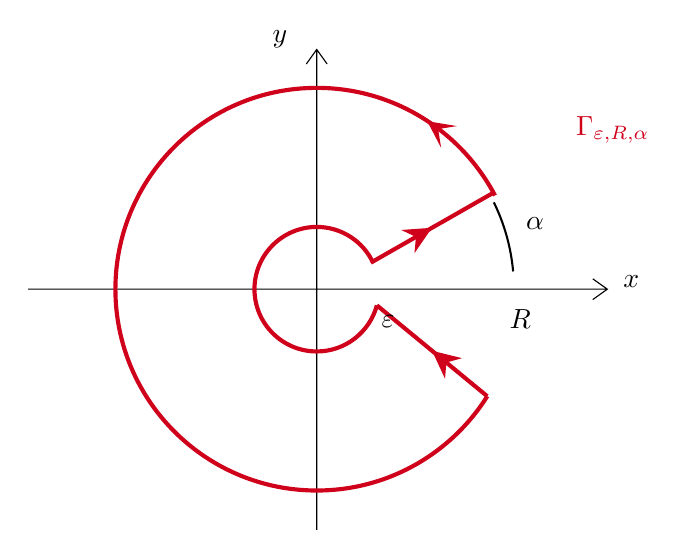
\begin{tikzpicture}[x=0.75pt,y=0.75pt,yscale=-1,xscale=1]
%uncomment if require: \path (0,253); %set diagram left start at 0, and has height of 253

%Shape: Axis 2D [id:dp4977301214304819] 
\draw  (162.5,130.13) -- (441.5,130.13)(301.5,14.63) -- (301.5,246.13) (434.5,125.13) -- (441.5,130.13) -- (434.5,135.13) (296.5,21.63) -- (301.5,14.63) -- (306.5,21.63)  ;
%Straight Lines [id:da9935131902630598] 
\draw [color={rgb, 255:red, 208; green, 2; blue, 27 }  ,draw opacity=1 ][line width=1.5]    (327.56,117.36) -- (386.5,83.73) ;
\draw [shift={(357.03,100.55)}, rotate = 510.29] [fill={rgb, 255:red, 208; green, 2; blue, 27 }  ,fill opacity=1 ][line width=0.08]  [draw opacity=0] (13.4,-6.43) -- (0,0) -- (13.4,6.44) -- (8.9,0) -- cycle    ;
%Shape: Arc [id:dp13640780925563867] 
\draw  [draw opacity=0][line width=1.5]  (330.48,137.92) .. controls (327.04,150.71) and (315.37,160.13) .. (301.5,160.13) .. controls (284.93,160.13) and (271.5,146.69) .. (271.5,130.13) .. controls (271.5,113.56) and (284.93,100.13) .. (301.5,100.13) .. controls (313.42,100.13) and (323.72,107.08) .. (328.56,117.16) -- (301.5,130.13) -- cycle ; \draw  [color={rgb, 255:red, 208; green, 2; blue, 27 }  ,draw opacity=1 ][line width=1.5]  (330.48,137.92) .. controls (327.04,150.71) and (315.37,160.13) .. (301.5,160.13) .. controls (284.93,160.13) and (271.5,146.69) .. (271.5,130.13) .. controls (271.5,113.56) and (284.93,100.13) .. (301.5,100.13) .. controls (313.42,100.13) and (323.72,107.08) .. (328.56,117.16) ;
%Shape: Arc [id:dp11391386463291964] 
\draw  [draw opacity=0][line width=1.5]  (383.66,181.71) .. controls (366.5,208.99) and (336.12,227.13) .. (301.5,227.13) .. controls (247.93,227.13) and (204.5,183.7) .. (204.5,130.13) .. controls (204.5,76.55) and (247.93,33.13) .. (301.5,33.13) .. controls (338.77,33.13) and (371.13,54.15) .. (387.38,84.98) -- (301.5,130.13) -- cycle ; \draw  [color={rgb, 255:red, 208; green, 2; blue, 27 }  ,draw opacity=1 ][line width=1.5]  (383.66,181.71) .. controls (366.5,208.99) and (336.12,227.13) .. (301.5,227.13) .. controls (247.93,227.13) and (204.5,183.7) .. (204.5,130.13) .. controls (204.5,76.55) and (247.93,33.13) .. (301.5,33.13) .. controls (338.77,33.13) and (371.13,54.15) .. (387.38,84.98) ;
%Straight Lines [id:da9801209891079499] 
\draw [color={rgb, 255:red, 208; green, 2; blue, 27 }  ,draw opacity=1 ][line width=1.5]    (383.66,181.71) -- (330.48,137.92) ;
\draw [shift={(357.07,159.81)}, rotate = 399.46000000000004] [fill={rgb, 255:red, 208; green, 2; blue, 27 }  ,fill opacity=1 ][line width=0.08]  [draw opacity=0] (13.4,-6.43) -- (0,0) -- (13.4,6.44) -- (8.9,0) -- cycle    ;
\draw  [draw opacity=0][fill={rgb, 255:red, 208; green, 2; blue, 27 }  ,fill opacity=1 ] (361.45,62.08) -- (354.73,49.18) -- (369.08,51.55) -- (360,53) -- cycle ;
%Shape: Arc [id:dp2448048568760779] 
\draw  [draw opacity=0][line width=0.75]  (386.82,88.29) .. controls (391.83,98.49) and (395.06,109.72) .. (396.12,121.58) -- (301.5,130.13) -- cycle ; \draw  [color={rgb, 255:red, 0; green, 0; blue, 0 }  ,draw opacity=1 ][line width=0.75]  (386.82,88.29) .. controls (391.83,98.49) and (395.06,109.72) .. (396.12,121.58) ;

% Text Node
\draw (393.18,138.47) node [anchor=north west][inner sep=0.75pt]    {$R$};
% Text Node
\draw (448,122.4) node [anchor=north west][inner sep=0.75pt]    {$x$};
% Text Node
\draw (279,4.4) node [anchor=north west][inner sep=0.75pt]    {$y$};
% Text Node
\draw (331.48,141.52) node [anchor=north west][inner sep=0.75pt]    {$\varepsilon $};
% Text Node
\draw (425.18,45.47) node [anchor=north west][inner sep=0.75pt]  [color={rgb, 255:red, 208; green, 2; blue, 27 }  ,opacity=1 ]  {$\Gamma _{\varepsilon ,R,\alpha }$};
% Text Node
\draw (401.18,94.47) node [anchor=north west][inner sep=0.75pt]    {$\alpha $};


\end{tikzpicture}
\end{figure}
\FloatBarrier

Dobbiamo usare la determinazione del logaritmo che esclude l'asse reale positivo
\begin{equation*}
\mathrm{Log}_{\left( 2\pi \right)} :=\ln z+i\vartheta \ \ \ \ \vartheta \in \arg z\cap \left( 0,2\pi \right)
\end{equation*}
Si considera rispettivamente
\begin{equation*}
\begin{array}{ c l }
A & f\left( z\right) =e^{\alpha \cdotp \mathrm{Log}_{\left( 2\pi \right)} z} R\left( z\right)\\
B & f\left( z\right) =\mathrm{Log}_{\left( 2\pi \right)} z\cdotp R\left( z\right)\\
C & f\left( z\right) =\left(\mathrm{Log}_{\left( 2\pi \right)} z\right)^{2} R\left( z\right)
\end{array}
\end{equation*}


Calcolare


\begin{equation*}
I=\int ^{+\infty }_{0}\frac{1}{\sqrt{x}\left( 1+x\right)} dx=\int ^{+\infty }_{0}\frac{x^{-1/2}}{\left( 1+x\right)} dx
\end{equation*}
\Esercizio{}

Calcolare
\begin{equation*}
I=\int ^{+\infty }_{0}\frac{1}{\left( x^{2} +4\right)\left( x+1\right)} dx
\end{equation*}
\Esercizio{(Spazi $L^{p}$)}

Si considerino le seguenti funzioni definite su $\left( 0,+\infty \right)$ nel seguente modo
\begin{equation*}
f\left( x\right) =\frac{1}{\sqrt{x}} \ \ \ \ g\left( x\right) =\frac{1}{\sqrt{x+1}}
\end{equation*}
\begin{enumerate}
\item Stabilire per quali $p\in \left[ 1,+\infty \right]$ le seguenti funzioni stanno in $L^{p}\left( 1,+\infty \right)$:\begin{equation*}
f\ \ \ \ g\ \ \ \ f-g\ \ \ \ \frac{g}{f}
\end{equation*}
\item Stessa domanda in $\left( 0,1\right)$
\end{enumerate}
\Esercizio{ }

Sia $B=\left\{\left( x,y\right) \in \mathbb{R}^{2} :x^{2} +y^{2} \leqslant 1\right\}$ e sia
\begin{equation*}
f\left( x,y\right) =\frac{1}{\sqrt{x^{2} +y^{2}}}
\end{equation*}
\begin{enumerate}
\item Stabilire per quali $p\geqslant 1$ si ha $f\in L^{p}\left( B\right)$
\item Stabilire per quali $q$ si ha $f\in L^{q}\left(\mathbb{R}^{2} \setminus B\right)$.
\end{enumerate}
\Esercizio{}

Sia
\begin{equation*}
f_{n}\left( x\right) =\frac{n^{2}\sin\left(\frac{x^{2}}{n^{2}}\right)}{\left( x^{2} +n^{2}\right)^{3/2}\log^{3/2}\left( x^{2} +n^{2}\right)} \ \ n\in \mathbb{N}
\end{equation*}
Rispondere ai seguenti quesiti
\begin{enumerate}
\item Per quali $n\in \mathbb{N}$ si ha $f_{n} \in L^{1}\left( 0,+\infty \right)$.
\item Determinare la funzione limite $f$ in $\left( 0,+\infty \right)$.
\item Calcolare $\lim\limits _{n\rightarrow +\infty }\int ^{+\infty }_{0} f_{n}\left( x\right) dx$
\end{enumerate}
\Esercizio{}

Date le $f_{n}\left( x\right) =\arctan\left( nx\right)$ definite su $\left[ 0,+\infty \right)$. 
\begin{enumerate}
\item Determinare il limite puntuale $f\left( x\right)$
\item Stabilire se $f_{n}\rightarrow f$ in $L^{p}\left( 0,+\infty \right)$ per $p\in \left[ 1,+\infty \right)$.
\end{enumerate}
\ParteSoluzioni
\Soluzione

$f_{\alpha } \sim x^{\alpha -3} \ \ x\rightarrow +\infty $.

$f_{\alpha }$ è integrabile in un intorno di $+\infty $ se e solo se $3-\alpha  >1$, cioè $\Leftrightarrow \alpha < 2$.

$f_{\alpha } \sim x^{\alpha } \ \ x\rightarrow 0^{+}$.

$f_{\alpha }$ è integrabile in senso proprio in un intorno destro di $0$ $\Leftrightarrow -\alpha < 1\Leftrightarrow \alpha  >-1$.

$\Rightarrow \exists I$ se e solo se $-1< \alpha < 2$.



Sia $f\left( z\right) =\frac{e^{\alpha \log z}}{1+z^{3}}$.

Considero un angolo $=\frac{2\pi }{m} =\frac{2\pi }{3}$


\begin{figure}[htpb]
	\centering
\tikzset{every picture/.style={line width=0.75pt}} %set default line width to 0.75pt        

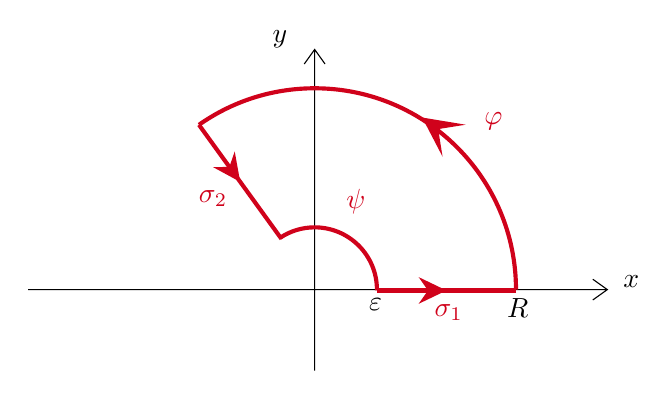
\begin{tikzpicture}[x=0.75pt,y=0.75pt,yscale=-1,xscale=1]
%uncomment if require: \path (0,193); %set diagram left start at 0, and has height of 193

%Shape: Axis 2D [id:dp38802361743556224] 
\draw  (162.5,140.33) -- (441.5,140.33)(300.5,24.63) -- (300.5,179.33) (434.5,135.33) -- (441.5,140.33) -- (434.5,145.33) (295.5,31.63) -- (300.5,24.63) -- (305.5,31.63)  ;
%Straight Lines [id:da7713867715877043] 
\draw [color={rgb, 255:red, 208; green, 2; blue, 27 }  ,draw opacity=1 ][line width=1.5]    (330.5,140.75) -- (397.5,140.75) ;
\draw [shift={(364,140.75)}, rotate = 180] [fill={rgb, 255:red, 208; green, 2; blue, 27 }  ,fill opacity=1 ][line width=0.08]  [draw opacity=0] (13.4,-6.43) -- (0,0) -- (13.4,6.44) -- (8.9,0) -- cycle    ;
%Shape: Arc [id:dp12128862418563902] 
\draw  [draw opacity=0][line width=1.5]  (283.84,115.38) .. controls (288.61,112.19) and (294.34,110.33) .. (300.5,110.33) .. controls (317.07,110.33) and (330.5,123.76) .. (330.5,140.33) .. controls (330.5,140.47) and (330.5,140.61) .. (330.5,140.75) -- (300.5,140.33) -- cycle ; \draw  [color={rgb, 255:red, 208; green, 2; blue, 27 }  ,draw opacity=1 ][line width=1.5]  (283.84,115.38) .. controls (288.61,112.19) and (294.34,110.33) .. (300.5,110.33) .. controls (317.07,110.33) and (330.5,123.76) .. (330.5,140.33) .. controls (330.5,140.47) and (330.5,140.61) .. (330.5,140.75) ;
%Shape: Arc [id:dp7213752730044614] 
\draw  [draw opacity=0][line width=1.5]  (244.75,60.94) .. controls (260.52,49.84) and (279.75,43.33) .. (300.5,43.33) .. controls (354.07,43.33) and (397.5,86.76) .. (397.5,140.33) -- (300.5,140.33) -- cycle ; \draw  [color={rgb, 255:red, 208; green, 2; blue, 27 }  ,draw opacity=1 ][line width=1.5]  (244.75,60.94) .. controls (260.52,49.84) and (279.75,43.33) .. (300.5,43.33) .. controls (354.07,43.33) and (397.5,86.76) .. (397.5,140.33) ;
%Straight Lines [id:da09050365562806317] 
\draw [color={rgb, 255:red, 208; green, 2; blue, 27 }  ,draw opacity=1 ][line width=1.5]    (244.75,60.94) -- (284.5,115.89) ;
\draw [shift={(264.62,88.42)}, rotate = 234.12] [fill={rgb, 255:red, 208; green, 2; blue, 27 }  ,fill opacity=1 ][line width=0.08]  [draw opacity=0] (13.4,-6.43) -- (0,0) -- (13.4,6.44) -- (8.9,0) -- cycle    ;
\draw  [draw opacity=0][fill={rgb, 255:red, 208; green, 2; blue, 27 }  ,fill opacity=1 ] (362.12,76.27) -- (352.31,57.43) -- (373.27,60.88) -- (360,63) -- cycle ;

% Text Node
\draw (392,143.4) node [anchor=north west][inner sep=0.75pt]    {$R$};
% Text Node
\draw (448,132.4) node [anchor=north west][inner sep=0.75pt]    {$x$};
% Text Node
\draw (279,14.4) node [anchor=north west][inner sep=0.75pt]    {$y$};
% Text Node
\draw (325.5,143.4) node [anchor=north west][inner sep=0.75pt]    {$\varepsilon $};
% Text Node
\draw (381,53.9) node [anchor=north west][inner sep=0.75pt]  [color={rgb, 255:red, 208; green, 2; blue, 27 }  ,opacity=1 ]  {$\varphi $};
% Text Node
\draw (314.5,90.9) node [anchor=north west][inner sep=0.75pt]  [color={rgb, 255:red, 208; green, 2; blue, 27 }  ,opacity=1 ]  {$\psi $};
% Text Node
\draw (243.5,91.4) node [anchor=north west][inner sep=0.75pt]  [color={rgb, 255:red, 208; green, 2; blue, 27 }  ,opacity=1 ]  {$\sigma _{2}$};
% Text Node
\draw (357,146.4) node [anchor=north west][inner sep=0.75pt]  [color={rgb, 255:red, 208; green, 2; blue, 27 }  ,opacity=1 ]  {$\sigma _{1}$};


\end{tikzpicture}
\end{figure}
\FloatBarrier

Chiamo l'intera curva $\gamma _{R,\varepsilon } =\sigma _{1} \cup \varphi \cup \sigma _{2} \cup \psi $

Per il teorema dei residui
\begin{equation*}
\int _{\gamma _{R,\varepsilon }} f\left( z\right) dz=2\pi i\cdotp \mathrm{Res}\left( f,e^{i\pi /3}\right)
\end{equation*}
$e^{i\pi /3}$ è l'unico punto interno alla curva in cui si annulla il denominatore.
\begin{equation*}
\begin{aligned}
\int _{\gamma _{R,\varepsilon }} & =\int _{\sigma _{1}} +\int _{\varphi } +\int _{\sigma _{2}} +\int _{\psi }\\
 & \\
\int _{\sigma _{1}} & =\left\{\begin{array}{ c }
z=t\\
t\in [ \varepsilon ,R]
\end{array}\right\} =\int ^{R}_{\varepsilon }\frac{e^{\alpha \ln t}}{1+t^{3}} dt\xrightarrow[R\rightarrow +\infty ]{\varepsilon \rightarrow 0^{+}} I\\
 & \\
\int _{\sigma _{2}} & =\left\{\begin{array}{ c }
z=te^{i2\pi /3}\\
t\in [ \varepsilon ,R]
\end{array}\right\} =-\int ^{R}_{\varepsilon }\frac{e^{\alpha \ln te^{i2\pi /3}}}{1+t^{3}} e^{i2\pi /3} dt=-\int ^{R}_{\varepsilon }\frac{e^{\alpha \left(\ln t+\ln e^{i2\pi /3}\right)}}{1+t^{3}} e^{i2\pi /3} dt\\
 & =-\int ^{R}_{\varepsilon }\frac{e^{\alpha (\ln t+i2\pi /3)}}{1+t^{3}} e^{i2\pi /3} dt=-e^{i\frac{2}{3} \pi ( 1+\alpha )}\int ^{R}_{\varepsilon }\frac{e^{\alpha \ln t}}{1+t^{3}} dt\\
 & \xrightarrow[R\rightarrow +\infty ]{\varepsilon \rightarrow 0^{+}} -e^{i\frac{2}{3} \pi ( 1+\alpha )} I\\
 & \\
\left| \int _{\varphi }\right|  & =\left\{\begin{array}{ c }
z=Re^{it}\\
t\in [ 0,2\pi /3]
\end{array}\right\} =\left| \int ^{2\pi /3}_{0}\frac{e^{\alpha (\ln R+it)}}{1+R^{3} e^{i3t}}\textcolor[rgb]{0.29,0.56,0.89}{\underbrace{Rie^{it}}_{\gamma '}} dt\right| =\int ^{2\pi /3}_{0}\frac{\left| e^{\alpha (\ln R+it)}\right| }{\left| 1+R^{3} e^{i3t}\right| }\textcolor[rgb]{0.82,0.01,0.11}{\left| Rie^{it}\right| } dt\\
 & \textcolor[rgb]{0.96,0.65,0.14}{| | a| -| b| | \leqslant | a+b| \leqslant | a| +| b| }\\
 & \leqslant \int ^{2\pi /3}_{0}\frac{\left| e^{\alpha (\ln R+it)}\right| }{\left| 1-R^{3}\right| }\textcolor[rgb]{0.82,0.01,0.11}{R} dt\leqslant \frac{R^{\alpha +1}}{\left| 1-R^{3}\right| }\frac{2\pi }{3} dt\sim \frac{2\pi }{3}\frac{1}{R^{2-\alpha }}\xrightarrow[\alpha \in ( -1,2)]{R\rightarrow +\infty } 0\\
 & \\
\left| \int _{\psi }\right|  & =\left\{\begin{array}{ c }
z=\varepsilon e^{it}\\
t\in [ 0,2\pi /3]
\end{array}\right\} =\left| \int ^{2\pi /3}_{0}\frac{e^{\alpha (\ln \varepsilon +it)}}{1+\varepsilon ^{3} e^{i3t}}\textcolor[rgb]{0.29,0.56,0.89}{\underbrace{\varepsilon ie^{it}}_{\gamma '}} dt\right| \leqslant \dotsc \leqslant \frac{2\pi }{3} \varepsilon ^{\alpha +1}\xrightarrow[\alpha \in ( -1,2)]{\varepsilon \rightarrow 0^{+}} 0\\
 & \\
\Rightarrow  & \ \ \frac{2\pi i\cdotp \mathrm{Res}\left( f,e^{i\pi /3}\right)}{1-e^{i\frac{2}{3} \pi ( 1+\alpha )}} =I
\end{aligned}
\end{equation*}
Resta solo da calcolare il residuo.
\Soluzione

Devo considerare la forma $A$
\begin{gather*}
f( z) =e^{-\frac{1}{2}\mathrm{Log}_{( 2\pi )} z} \cdotp \frac{1}{1+z}\\
\int _{\gamma _{\varepsilon ,R}} f( z) dz=2\pi i\cdotp \sum \mathrm{Res}( f) =2\pi i\cdotp \mathrm{Res}( f,-1)
\end{gather*}
Ugualmente
\begin{equation*}
\begin{aligned}
\int _{\gamma _{R,\varepsilon }} & =\int _{\sigma _{1}} +\int _{\varphi } +\int _{\sigma _{2}} +\int _{\psi }\\
 & \\
\int _{\sigma _{1} \cup \sigma _{2}} & =\left\{\begin{array}{ c }
z=t\\
t\in [ \varepsilon ,R]
\end{array}\right\} =\int ^{R}_{\varepsilon }\frac{1}{1+t}\left[ e^{-\frac{1}{2}\ln t} -e^{-\frac{1}{2}(\ln t+2\pi i)}\right] dt\\
 & =\underbrace{\left( 1-e^{-\pi i}\right)}_{1+1=2}\int ^{R}_{\varepsilon }\frac{1}{\sqrt{t}( 1+t)} dt\xrightarrow[R\rightarrow +\infty ]{\varepsilon \rightarrow 0^{+}} 2I\\
 & \\
\int _{\varphi } & \xrightarrow{R\rightarrow +\infty } 0\\
\int _{\psi } & \xrightarrow{\varepsilon \rightarrow 0^{+}} 0\\
 & \\
\Rightarrow  & \ \ 2I=2\pi i\cdotp \mathrm{Res}( f,-1) \ \ \Rightarrow \ \ I=\pi i\cdotp \mathrm{Res}( f,-1)
\end{aligned}
\end{equation*}
\Soluzione

Siamo nel caso $B$
\begin{gather*}
f\left( z\right) =\mathrm{Log}_{\left( 2\pi \right)} z\cdotp R\left( z\right) =f\left( z\right) =\frac{\mathrm{Log}_{\left( 2\pi \right)} z}{\left( z^{2} +4\right)\left( z+1\right)}\\
\int _{\gamma _{\varepsilon ,R}} f\left( z\right) dz=2\pi i\cdotp \sum \mathrm{Res}\left( f,z_{i}\right)
\end{gather*}
Il denominatore si annulla per $z=-1,\pm 2i$.
\begin{equation*}
\begin{aligned}
\int _{\gamma _{R,\varepsilon }} & =\int _{\sigma _{1}} +\int _{\varphi } +\int _{\sigma _{2}} +\int _{\psi }\\
 & \\
\int _{\sigma _{1} \cup \sigma _{2}} & =\left\{\begin{array}{ c }
z=t\\
t\in \left[ \varepsilon ,R\right]
\end{array}\right\} =\int ^{R}_{\varepsilon }\frac{1}{\left( t+1\right)\left( t^{2} +4\right)}\left[\ln t-\left(\ln t+2\pi i\right)\right] dt\xrightarrow[R\rightarrow +\infty ]{\varepsilon \rightarrow 0^{+}} -2\pi iI\\
 & \\
\int _{\varphi } & \xrightarrow{R\rightarrow +\infty } 0\\
\int _{\psi } & \xrightarrow{\varepsilon \rightarrow 0^{+}} 0
\end{aligned}
\end{equation*}
\Soluzione

Rispondiamo al punto $1$.
\begin{equation*}
\ \begin{aligned}
\left| f\left( x\right)\right| ^{p} & =\frac{1}{x^{p/2}} \ \ \Rightarrow \ \ f\in L^{p}\left( 1,+\infty \right) \ \ \Leftrightarrow \ \ \frac{p}{2}  >1\ \ \Leftrightarrow \ \ p >2\ \left( +\infty \ \text{incluso}\right)\\
 & \\
\left| g\left( x\right)\right| ^{p} & =\frac{1}{\left( x+1\right)^{p/2}}\overset{x\rightarrow +\infty }{\sim }\frac{1}{x^{p/2}} \ \ \Rightarrow \ \ g\in L^{p}\left( 1,+\infty \right) \ \ \Leftrightarrow \ \ p >2\ \left( +\infty \ \text{incluso}\right)\\
 & \\
\left| f-g\right| ^{p} & =\left| \frac{1}{\sqrt{x}} -\frac{1}{\sqrt{x+1}}\right| ^{p} =\left| \frac{\sqrt{x+1} -\sqrt{x}}{\sqrt{x}\sqrt{x+1}}\right| ^{p}\\
 & =\left| \frac{\sqrt{x+1} -\sqrt{x}}{\sqrt{x^{2} +x}} \cdotp \frac{\sqrt{x+1} +\sqrt{x}}{\sqrt{x+1} +\sqrt{x}}\right| ^{p} =\left| \frac{x+1-x}{\sqrt{x^{2} +x}\left(\sqrt{x+1} +\sqrt{x}\right)}\right| ^{p}\\
 & =\left| \frac{x+1-x}{\sqrt{x^{2} +x}\left(\sqrt{x+1} +\sqrt{x}\right)}\right| ^{p}\overset{x\rightarrow +\infty }{\sim }\left| \frac{1}{x\left( 2\sqrt{x}\right)}\right| ^{p} =\frac{1}{2^{p} x^{3p/2}}\\
 & \Rightarrow \ \ f-g\in L^{p}\left( 1,+\infty \right) \ \ \Leftrightarrow \ \ \frac{3}{2} p >1\ \ \Leftrightarrow \ \ p >\frac{2}{3} \ \text{cioè il primo intero:} \ p\geqslant 1\\
 & \\
\frac{g\left( x\right)}{f\left( x\right)} & \overset{x\rightarrow +\infty }{\sim } 1\ \ \Rightarrow \ \ \frac{g}{f} \in L^{p}\left( 1,+\infty \right) \ \ \Leftrightarrow \ \ p=+\infty 
\end{aligned}
\end{equation*}
Rispondiamo al punto $2$.
\begin{equation*}
| f( x)| ^{p}\overset{x\rightarrow 0^{+}}{\sim }\frac{1}{x^{p/2}} \ \ \Rightarrow \ \ f\in L^{p}( 0,1) \ \ \Leftrightarrow \ \ \frac{p}{2} < 1\ \ \Leftrightarrow \ \ 1\leqslant p< 2
\end{equation*}
$g$ è limitata in $( 0,1) \Rightarrow g\in L^{p}( 0,1) \ \forall p\geqslant 1$, incluso $+\infty $.

$f-g\in L^{p}( 0,1) \Leftrightarrow 1\leqslant p< 2$ dato che so sommando due funzioni, di cui una limitata su intervallo limitato che non presenta problemi e una in $L^{p}$ per $1\leqslant p< 2$.

$\frac{g}{f} \in L^{p}( 0,1) \ \forall p\geqslant 1$, incluso $+\infty $.
\Soluzione

Rispondiamo al punto $1$.

Passiamo in coordinate polari centrate nell'origine
\begin{gather*}
\begin{cases}
x=\rho \cos \vartheta \\
y=\rho \sin \vartheta 
\end{cases} \ \ \Rightarrow \ \ \iint _{B}| f( x,y)| ^{p} dxdy=\iint _{B^{\star }}\left| \frac{1}{\rho }\right| ^{p} \rho d\rho d\vartheta \\
\\
B^{\star } =\{( \rho ,\vartheta ) :0\leqslant \rho \leqslant 1,0< \vartheta < 2\pi \}\\
\\
\int ^{2\pi }_{0} d\vartheta \int ^{1}_{0}\frac{1}{\rho ^{p-1}} d\rho < +\infty \ \ \Leftrightarrow \ \ p-1< 1\ \ \Leftrightarrow \ \ p< 2\land p\geqslant 1
\end{gather*}
Rispondiamo al punto $2$.
\begin{gather*}
\iint _{\mathbb{R}^{2} \setminus B}| f( x,y)| ^{q} dxdy=2\pi \int ^{+\infty }_{1}\frac{1}{\rho ^{q-1}} d\rho < +\infty \ \ \Leftrightarrow \ \ q-1 >1\\
\Leftrightarrow q >2\ \left( +\infty \ \text{incluso}\right)
\end{gather*}
\Soluzione
\begin{theorem}
[della convergenza dominata] Sia $\{f_{n}\}$ una successione di funzioni misurabili su un insieme $\Omega \subset \mathbb{R}^{n}$ misurabile. Supponiamo che siano verificate le seguenti due condizioni:\footnote{È importante che la $g$ non dipenda da $n$.}
\begin{equation*}
\begin{cases}
f_{n}\xrightarrow{n\rightarrow +\infty } f\ \text{q.o. in} \ \Omega \\
\exists g\in L^{1}( \Omega ) :| f_{n}| \leqslant g( x) \ \text{per q.o.} \ x\in \Omega ,\ \forall n\in \mathbb{N}
\end{cases}
\end{equation*}
Allora
\begin{equation*}
f\in L^{1}( \Omega ) ,\ \ \ \ \lim _{n\rightarrow +\infty }\int _{\Omega } f_{n}( x) dx=\int _{\Omega }\lim _{n\rightarrow +\infty } f_{n}( x) dx
\end{equation*}
\end{theorem}
\begin{enumerate}
\item Le $f_{n}$ sono continue su $E=( 0,+\infty )$ e quindi misurabili su $E$

$\forall n >0$ fissato si ha\begin{equation*}
| f_{n}( x)| \leqslant \frac{n^{2}}{\left( x^{2}\right)^{3/2}\log^{3/2}\left( x^{2}\right)} =\frac{n^{2}}{x^{3}( 2\log x)^{3/2}} =\frac{n^{2}}{2^{3/2} x^{3}(\log x)^{3/2}} \ \ x\rightarrow +\infty 
\end{equation*}

$f_{n}$ è integrabile nell'intorno di $+\infty ,\forall n >0$.\begin{equation*}
\text{per} \ x\rightarrow 0\ \ f( x) \sim \begin{cases}
\frac{x^{2}}{n^{3}\log^{3/2}\left( n^{2}\right)} , & n\geqslant 2\\
\frac{x^{2}}{\log^{3/2}\left( x^{2} +1\right)} \sim \frac{x^{2}}{x^{3}} =\frac{1}{x} , & n=1
\end{cases}
\end{equation*}

$f_{n}$ sono integrabili in $U\left( 0^{+}\right) ,\forall n\geqslant 2$.

$\Rightarrow f_{n} \in L^{1}( 0,+\infty ) \Leftrightarrow n\geqslant 2$.
\item Calcoliamo\begin{equation*}
\begin{aligned}
\lim _{n\rightarrow +\infty } f_{n}( x_{0}) & =\left\{x_{0} \ \text{è fissato}\right\}\\
 & =\lim _{n\rightarrow +\infty }\frac{n^{2}\sin\left(\frac{x^{2}_{0}}{n^{2}}\right)}{\left( x^{2}_{0} +n^{2}\right)^{3/2}\log^{3/2}\left( x^{2}_{0} +n^{2}\right)}\\
 & =\lim _{n\rightarrow +\infty }\frac{x^{2}_{0}}{n^{3}\log^{3/2}\left( n^{2}\right)} =0
\end{aligned}
\end{equation*}

$f_{n}$ converge puntualmente alla funzione limite $f( x) \equiv 0$.
\item Osservo\begin{equation*}
| \sin x| \leqslant x\ \ \forall x\in ( 0,+\infty ) \ \ \Rightarrow \ \ n^{2}\sin\left(\frac{x^{2}}{n^{2}}\right) \leqslant n^{2}\frac{x^{2}}{n^{2}} =x^{2}
\end{equation*}

Per $n\geqslant 2$\begin{equation*}
| f_{n}( x)| \leqslant g( x) :=\frac{x^{2}}{\left( x^{2} +2^{2}\right)^{3/2}\log^{3/2}\left( x^{2} +2^{2}\right)} \in L^{1}( 0,+\infty )
\end{equation*}
\begin{enumerate}
\item diminuisco il denominatore
\item devo ottenere qualcosa che \underline{\textbf{non dipende}} da $n$
\end{enumerate}

$\overset{\text{Dom}}{\Rightarrow }\lim\limits _{n\rightarrow +\infty }\int ^{+\infty }_{0} f_{n}( x) dx=\int ^{+\infty }_{0}\lim\limits _{n\rightarrow +\infty } f_{n}( x) dx=0$.
\end{enumerate}
\Soluzione
\begin{definition}
\begin{equation*}
f_{n}\xrightarrow[n\rightarrow +\infty ]{L^{p}} f\ ( p\in [ 1,+\infty )) \ \ \Leftrightarrow \ \ \Vert f_{n} -f\Vert ^{p}_{L^{p}}\xrightarrow{n\rightarrow +\infty } 0
\end{equation*}
\end{definition}
\begin{enumerate}
\item Fisso $x_{0} \in [ 0,+\infty )$
\begin{enumerate}
\item se $x_{0} =0\ \ \Rightarrow \ \ f_{n}( 0) =0$
\item se $x_{0} \neq 0\ \ \Rightarrow \ \ \lim\limits _{n\rightarrow +\infty } f_{n}( x) =\frac{\pi }{2}$
\end{enumerate}

$\Rightarrow \ \ \{f_{n}\}_{n\in \mathbb{N}}$ converge puntualmente a $f( x) =\begin{cases}
0, & x=0\\
\pi /2, & x\neq 0
\end{cases}$

\fg{0.7}{08-7}
\item Se $x >0$\begin{gather*}
f( x) -f_{n}( x) =\frac{\pi }{2} -\arctan( nx) =\arctan\left(\frac{1}{nx}\right)\\
\Rightarrow \ \ \Vert f_{n} -f\Vert ^{p}_{L^{p}} =\int ^{+\infty }_{0}\left(\arctan\left(\frac{1}{nx}\right)\right)^{p} dx
\end{gather*}

Escludo $p=1$, perché $\arctan\left(\frac{1}{nx}\right) \sim \frac{1}{nx}$ e $\frac{1}{x}$ non è integrabile a $+\infty $.

Verifichiamo le ipotesi della convergenza dominata.\begin{equation*}
\left| \left(\arctan\left(\frac{1}{nx}\right)\right)^{p}\right| \leqslant g( x) :=\begin{cases}
\left(\frac{\pi }{2}\right)^{p} , & 0< x< 1\ \left(\text{integrabile in zero} \ \forall p\right)\\
\left| \frac{1}{x}\right| ^{p} & x\geqslant 1\ \left(\text{uso proprio} \ n=1\ \text{per maggiorare}\right)
\end{cases}
\end{equation*}

$\overset{\text{Dom}}{\Rightarrow }\lim\limits _{n\rightarrow +\infty }\Vert f_{n} -f\Vert ^{p}_{L^{p}} =\lim\limits _{n\rightarrow +\infty }\int ^{+\infty }_{0}\left(\arctan\left(\frac{1}{nx}\right)\right)^{p} dx=\int ^{+\infty }_{0}\lim\limits _{n\rightarrow +\infty }\left(\arctan\left(\frac{1}{nx}\right)\right)^{p} dx=0$
\end{enumerate}
\chapter{Esercitazione 5 - Boella}
\ParteEsercizi
\Esercizio{}

Studiare la convergenza di
\begin{equation*}
f( x,y) =\frac{1}{(x^{2} +y^{2} )^{\alpha }\sqrt{1+x^{2} +y^{2}}}
\end{equation*}
scegliendo $\alpha $ tale per cui:
\begin{itemize}
\item $f\in L^{1} (\mathbb{R} )$
\item $f\in L^{p} (\mathbb{R} )$
\item $f\in L^{\infty } (\mathbb{R} )$
\end{itemize}
\Esercizio{}

Studiare la convergenza (ovvero limite puntuale, limite in $L^{p}$, limite in $L^{\infty }$, della seguente serie di funzioni:
\begin{equation*}
f_{n} (x)=\pi -2\arctan (|x|^{n} )
\end{equation*}
\Esercizio{}

Analizzare la seguente serie:
\begin{equation*}
f(x)=\sum ^{\infty }_{n=1}\frac{n+1}{n^{4} +n}\sin (n\pi x)
\end{equation*}
\begin{itemize}
\item $f_{n} (x)\in L^{2}$?
\item Che periodo ha?
\item Si può dire qualcosa anche sulla continuità?
\end{itemize}
\Esercizio{}

Data una funzione $2\pi $-periodica
\begin{equation*}
f:[ 0,2\pi )\rightarrow \mathbb{R} \ \ \ \ f(x)=x
\end{equation*}
Determinare la sue serie di Fourier. Si riesce a ricondurre la serie ad una nota?
\Esercizio{}

Data una funzione $1$-periodica dispari
\begin{equation*}
f:[ 0,1]\rightarrow \mathbb{R} \ \ \ \ f(x)=x-x^{2}
\end{equation*}
Determinare la sue serie di Fourier.
\ParteSoluzioni
\Soluzione

Sicuramente non appartiene a $L^{\infty }$ a meno che $\alpha $ non sia negativo dato che se $\alpha $ è positivo questa funzione ha un asintoto verticale.

Per vedere se $f\in L^{1}$, posto che sia sempre positiva, basta integrarla su tutto il piano e passare in coordinate polari. Quindi dovrà convergere l'integrale doppio
\begin{gather*}
\int ^{2\pi }_{0} d\vartheta \int ^{+\infty }_{0}\underbrace{\frac{1}{\rho ^{2}\sqrt{1+\rho ^{2}}} \rho }_{g( \rho )} d\rho \\
\begin{aligned}
\rho \rightarrow 0, & \ \ g(\rho )\sim \frac{1}{\rho ^{2\alpha -1}} \ \ \Rightarrow \ \ 2\alpha -1< 1\ \ \Rightarrow \ \ \alpha < 1\\
\rho \rightarrow +\infty , & \ \ g(\rho )\sim \frac{1}{\rho ^{2\alpha }} \ \ \Rightarrow \ \ 2\alpha  >1\ \ \Rightarrow \ \ \alpha  >\frac{1}{2}
\end{aligned}
\end{gather*}
Quindi
\begin{equation*}
f(x,y)\in L^{1} (\mathbb{R}^{2} )\ \ \Leftrightarrow \ \ \frac{1}{2} < \alpha < 1
\end{equation*}
Se invece consideriamo il generico $L^{p}$ dobbiamo elevare alla $p$, ma non il $\rho $ dello Jacobiano
\begin{equation*}
g(\rho )=\frac{\rho }{\rho ^{2\alpha p}\left(\sqrt{1+\rho ^{2}}\right)^{p}}
\end{equation*}
Calcoliamo
\begin{equation*}
\begin{aligned}
\rho \rightarrow 0^{+} , & \ \ g(\rho )\sim \frac{1}{\rho ^{2\alpha p-1}} \ \ \Rightarrow \ \ 2\alpha p-1< 1\ \ \Rightarrow \ \ \alpha < \frac{1}{\rho }\\
\rho \rightarrow +\infty , & \ \ g(\rho )\sim \frac{1}{\rho ^{(2\alpha +1)p-1}} \ \ \Rightarrow \ \ (2\alpha +1)p-1 >1\ \ \Rightarrow \ \ \alpha  >\frac{1}{\rho } -\frac{1}{2}
\end{aligned}
\end{equation*}
Allora
\begin{equation*}
f(x,y)\in L^{p} (\mathbb{R}^{2} )\ \ \Leftrightarrow \ \ \frac{1}{p} -\frac{1}{2} < \alpha < \frac{1}{p}
\end{equation*}
\Soluzione

Vediamo come sono fatte le $f_{n}$.

\fg{0.7}{09-2}
\begin{equation*}
F(x)=\lim _{n\rightarrow \infty }\left[ \pi -2\arctan (|x|^{n} )\right] =\begin{cases}
\pi , & |x|< 1\\
\frac{\pi }{2} , & |x|=1\\
0, & |x| >1
\end{cases}
\end{equation*}
Il limite in $L^{\infty }$ è immediato in quanto tutte le funzioni $f_{n}$ sono continue e quindi anche il limite dovrebbe essere continuo. Visto che il limite, come abbiamo visto, non è quasi ovunque continuo la convergenza in $L^{\infty }$ non sussiste.

Inoltre, la norma della differenza
\begin{equation*}
\Vert f_{n} -F\Vert _{\infty } =\frac{\pi }{2} \nrightarrow 0
\end{equation*}
La funzione converge a $F( x)$ in $L^{1} ,L^{p}$? Con la definizione
\begin{equation*}
\begin{aligned}
\lim _{x\rightarrow +\infty }\frac{f_{n} (x)}{\left(\frac{1}{x}\right)^{\alpha }} & =\lim _{x\rightarrow +\infty }\frac{\pi -2\arctan (x^{n} )}{x^{-\alpha }}\\
 & \overset{\text{H}}{=}\lim _{x\rightarrow \infty }\frac{-2\frac{nx^{n-1}}{1+x^{2n}}}{-\alpha x^{-\alpha -1}} =\lim _{x\rightarrow \infty }\frac{2n}{\alpha }\frac{x^{-n-1}}{x^{-\alpha -1}} =\begin{cases}
\infty , & \alpha  >n\\
2, & \alpha =n\\
0, & \alpha < n
\end{cases}
\end{aligned}
\end{equation*}
Quindi tutte le funzioni stanno in $L^{p}$, ma in realtà la funzione con $n=1$ non sta in $L^{1}$ ma in \ $L^{p} ,p >1$.

Per la convergenza in norma $L^{p}$ controlliamo la norma
\begin{equation*}
\Vert f_{n} -F\Vert ^{p}_{L^{p}} =2\int ^{1}_{0} (\pi -f_{n} (x))^{p} dx+2\int ^{+\infty }_{1} (f_{n} (x))^{p} dx
\end{equation*}
Utilizziamo la convergenza dominata in maniera disinvolta, formalmente servirebbe una $h( x)$ che maggiori
\begin{equation*}
| g_{n}( x) -G( x)| \leqslant h( x)
\end{equation*}
in realtà basta meno, serve una $h( x)$ che maggiori
\begin{equation*}
| g_{n}( x)| < h( x)
\end{equation*}
dalla quale si può risalire a quella cercata con la disuguaglianza triangolare.

Scegliamo quindi
\begin{equation*}
h(x)=\begin{cases}
\pi , & |x|\leqslant 1\\
f_{2} (x), & |x| >1
\end{cases}
\end{equation*}
\Soluzione
\begin{itemize}
\item Se gli $a_{n}$ e i $b_{n}$ tendono a $0$ in maniera monotona, allora la serie converge salvo in $0,2\pi ,4\pi \dotsc $
\item Vale\begin{equation*}
\sum\limits ^{\infty }_{n=0}(| a_{n}| +| b_{n}| ) < \infty \ \ \Rightarrow \ \ \text{la serie converge a una funzione continua}
\end{equation*}
\end{itemize}

Usiamo il secondo risultato
\begin{equation*}
f( x) \sim \frac{1}{n^{3}} \ \ \Rightarrow \ \ \text{converge}
\end{equation*}
Nella serie compaiono il seno ed il coseno di $2\pi nx/T$, quindi $T=2$.

Essendo una serie di soli seni la funzione è una funzione dispari\footnote{se fosse stata una funzione di soli coseni allora la funzione sarebbe stata pari.}.

Se la deriviamo, spunta fuori un $n$, quindi va a zero come $\frac{1}{n^{2}}$, quindi anche la derivata è continua, ovvero la funzione è $C^{1}$. Non possiamo dire altro.
\Soluzione

Si può sviluppare in serie di Fourier perché $f\in L^{2}( 0,2\pi )$.\footnote{In alcuni libri una volta costruita la serie di Fourier si scrive 
\begin{equation*}
f(x)\sim \frac{a_{o}}{2} +\sum ...
\end{equation*}
dove il simbolo $\sim $ indica che alla funzione \textit{si associa} la serie di Fourier.}

Scriviamo la serie di Fourier della funzione
\begin{equation*}
\begin{aligned}
a_{0} & =\frac{1}{\pi }\int ^{2\pi }_{0} xdx=2\pi \\
a_{n} & =\frac{1}{\pi }\int ^{2\pi }_{0} x\cos (nx)dx\overset{\text{ipp}}{=}\frac{1}{\pi }\left\{\left[\frac{x}{n}\sin (nx)\right]^{2\pi }_{0} -\frac{1}{n}\int ^{2\pi }_{0}\sin (nx)dx\right\} =0\\
b_{n} & =\frac{1}{\pi }\int ^{2\pi }_{0} x\sin (nx)dx\overset{\text{ipp}}{=}\frac{1}{\pi }\left\{\left[ -\frac{x}{n}\cos (nx)\right]^{2\pi }_{0} -\frac{1}{n}\int ^{2\pi }_{0}\cos (nx)dx\right\} =-\frac{2}{n}
\end{aligned}
\end{equation*}
Possiamo allora dire che
\begin{equation*}
f(x)=\pi +\sum ^{+\infty }_{n=1} -\frac{2}{n}\sin (nx)
\end{equation*}
\fg{0.6}{09-4}

A seguito di questo esempio possiamo dire se converge la serie
\begin{equation*}
\sum ^{+\infty }_{n=1}\frac{\sin n}{n}
\end{equation*}
Basta calcolare
\begin{equation*}
1=f(1)=\pi -2\sum ^{\infty }_{n=1}\frac{\sin (n)}{n} \ \ \Rightarrow \ \ \sum ^{+\infty }_{n=1}\frac{\sin n}{n} =\frac{\pi -1}{2}
\end{equation*}
Altra cosa che possiamo utilizzare avendo la serie di Fourier è l'uguaglianza di Parseval: se una funzione sta in $L^{2}( 0,2\pi )$ \ sviluppata in serie di Fourier allora
\begin{equation*}
\int ^{2\pi }_{0} f(x)^{2} dx=\pi \left[\frac{a^{2}_{0}}{2} +\sum ^{+\infty }_{n=1}\left( a^{2}_{n} +b^{2}_{n}\right)\right]
\end{equation*}
Applicandola alla serie che abbiamo calcolato avremo che
\begin{equation*}
\begin{aligned}
\int ^{2\pi }_{0} x^{2} dx & =\pi \left[\frac{(2\pi )^{2}}{2} +\sum ^{+\infty }_{n=1}\frac{4}{n^{2}}\right]\\
\frac{8}{3} \pi ^{3} & =\pi \left[\frac{(2\pi )^{2}}{2} +\sum ^{+\infty }_{n=1}\frac{4}{n^{2}}\right]\\
 & \Rightarrow \ \ \sum ^{+\infty }_{n=1}\frac{1}{n^{2}} =\frac{\frac{8}{3} \pi ^{2} -2\pi ^{2}}{4} =\frac{\pi ^{2}}{6}
\end{aligned}
\end{equation*}
\Soluzione

Dal grafico vediamo che la sua funzione è continua.

Lo sarà anche la sua derivata? Si vede dal grafico che quando $x\rightarrow 0^{-}$ la funzione è asintotica a $x$ mentre quando $x\rightarrow 0^{+}$ la funzione è asintotica a $x$ ergo la derivata sarà continua. Non si può certo dire della sua derivata seconda in quanto nell'origine ci sarà un'oscillazione del segno della costante. È ragionevole aspettarci che i coefficienti della serie convergeranno come $1/x^{3}$.

Visto che la funzione è dispari sappiamo già che $a_{0} =a_{n} =0$
\begin{equation*}
f(x)=\sum ^{+\infty }_{n=1} b_{n}\sin (n\pi x)
\end{equation*}
Calcoliamo $b_{n}$

Usando le proprietà delle funzioni pari e il fatto che l'integrale possiamo farlo dove ci pare, purché di ampiezza uguale al periodo
\begin{equation*}
\begin{aligned}
b_{n} & =\frac{1}{T/2}\int ^{T}_{0} f(x)\sin\left(\frac{2\pi n}{T} x\right) dx=\int ^{1}_{-1} f(x)\sin( \pi nx) dx\\
 & =2\int ^{1}_{0} f(x)\sin( \pi nx) dx=2\int ^{1}_{0}\left( x-x^{2}\right)\sin( \pi nx) dx\\
 & \overset{\text{ipp}}{=} 2\left\{\cancel{\left[ -\frac{x-x^{2}}{n\pi }\cos( n\pi x)\right]^{1}_{0}} +\frac{1}{n\pi }\int ^{1}_{0}( 1-2x)\cos( n\pi x) dx\right\}\\
 & \overset{\text{ipp}}{=}\frac{2}{n\pi }\left\{\cancel{\left[\frac{1-2x}{n\pi }\sin( n\pi x)\right]^{1}_{0}} +\frac{2}{n\pi }\int ^{1}_{0}\sin( n\pi x) dx\right\}\\
 & =\frac{4}{n^{2} \pi ^{2}}\left[ -\frac{1}{n\pi }\cos (nx)\right]^{1}_{0} =\frac{4}{n^{3} \pi ^{3}}\left[ 1-( -1)^{n}\right] =\begin{cases}
0, & n\ \text{pari}\\
\frac{8}{n^{3} \pi ^{3}} , & n\ \text{dispari}
\end{cases}
\end{aligned}
\end{equation*}
In definitiva avremo, con $n=2k+1$
\begin{equation*}
f(x)=\sum ^{+\infty }_{n=1}\frac{4}{n^{3} \pi ^{3}} (1-( -1)^{n}\sin (n\pi x)=\sum ^{+\infty }_{k=0}\frac{8}{\pi ^{3} (2k+1)^{3}}\sin (\pi (2k+1)x)
\end{equation*}
\chapter{Esercitazione 5 - Potrich}
\ParteEsercizi
\Esercizio{}

Data la successione di funzioni $f_{n} :[ 0,+\infty )\rightarrow \mathbb{R}$
\begin{equation*}
f_{n}( x) =\sqrt{n} e^{-nx}
\end{equation*}
determinarne il limite puntuale e nelle norme $L^{1} ,L^{2} ,L^{\infty }$.
\Esercizio{}

Si consideri la successione di funzioni
\begin{equation*}
f_{n} (x)=\frac{2n^{2}\left( 1-\cos\frac{x}{n}\right)}{\left( 1+\frac{x}{n}\right)^{n}} ,\ \ x\in (0,+\infty )
\end{equation*}
\begin{enumerate}
\item Stabilire per quale $n\in \mathbb{N}$ si ha $f_{n} \in L^{1}(( 1,+\infty ))$ e per quale $n\in \mathbb{N}$ si ha 

$f_{n} \in L^{2}(( 1,+\infty ))$
\item Calcolare\begin{equation*}
\lim\limits _{n\rightarrow +\infty }\int ^{+\infty }_{0} f_{n}( x) dx\ \ \ \ \ \ \ \ \lim\limits _{n\rightarrow +\infty }\int ^{+\infty }_{0}[ f_{n}( x)]^{2} dx
\end{equation*}
\end{enumerate}
\Esercizio{}

Fissato $\alpha \in [ 0,4]$, consideriamo
\begin{equation*}
f_{n,\alpha }( x) =\frac{n^{\alpha }}{\left( x^{2} +n^{2}\right)\left( x^{2} +4n^{2}\right)}
\end{equation*}
\begin{enumerate}
\item Determinare il limite puntuale $F_{\alpha }( x)$.
\item Stabilire al variare di $\alpha $ se $f_{n,\alpha }\rightarrow F_{\alpha }$ in $L^{1}(\mathbb{R})$ e in $L^{\infty }(\mathbb{R})$.
\end{enumerate}
\Esercizio{}

Sia $f:\mathbb{R}\rightarrow \mathbb{R}$ la funzione $2\pi $-periodica che sull'intervallo $( -\pi ,\pi ]$ è definita da
\begin{equation*}
f( x) =x+| x| =\begin{cases}
2x, & x\in [ 0,\pi ]\\
0, & x\in ( -\pi ,0)
\end{cases}
\end{equation*}
\begin{enumerate}
\item Disegnare il grafico di $f$ in $[ -3\pi ,3\pi ]$
\item Stabilire per quali valori di $x\in \mathbb{R}$ la serie di Fourier $F$ di $f$ converge puntualmente, precisandone l'eventuale limite.
\item Calcolare la serie di Fourier $F$ di $f$.
\item Stabilire se $F$ converge in media quadratica a $f$.
\item Studiare la convergenza uniforme di $F$ a $f$
\end{enumerate}
\Esercizio{}

Si consideri la funzione
\begin{equation*}
f( x) =\cos\left(\sqrt{2} \cdotp x\right) \ \ \ \ \forall x\in \left[ -\frac{\pi }{2} ,\frac{\pi }{2}\right]
\end{equation*}
ripetuta periodicamente
\begin{enumerate}
\item Calcolare i coefficienti di Fourier di $f$.
\item Calcolare il valore di\begin{equation*}
\sum\limits ^{\infty }_{k=1}\frac{1}{2k^{2} -1}
\end{equation*}
\item Studiare la convergenza della serie (puntuale, in media quadratica, uniforme).
\end{enumerate}
\ParteSoluzioni
\Soluzione

Sia $x_{0} \in [ 0,+\infty )$ fissato
\begin{itemize}
\item Se $x_{0} =0,\ f_{n}( 0) =\sqrt{n}\xrightarrow{n\rightarrow +\infty } +\infty $
\item Se $x_{0}  >0,\ f_{n}( x_{0}) =\sqrt{n} e^{-nx_{0}}\xrightarrow{n\rightarrow +\infty } 0$
\end{itemize}
allora $\{f_{n}\}_{n\in \mathbb{N}}$ converge puntualmente alla funzione limite
\begin{equation*}
f( x) =\begin{cases}
+\infty , & x=0\\
0, & x\geqslant 0
\end{cases}
\end{equation*}
\fg{0.4}{10-1}
Studiamo la norma $L^{1}$
\begin{equation*}
\begin{aligned}
\| f_{n} -f\| _{1} & =\| f_{n} \| _{1} =\int ^{+\infty }_{0}\sqrt{n} e^{-nx} dx=\\
 & =\sqrt{n}\int ^{+\infty }_{0} e^{-nx} dx=\sqrt{n}\left[\frac{e^{-nx}}{-n}\right]^{+\infty }_{0} =\frac{1}{\sqrt{n}}\xrightarrow{n\rightarrow +\infty } 0\\
 & \Rightarrow \ \ f_{n}\xrightarrow[n\rightarrow +\infty ]{L^{1}} f
\end{aligned}
\end{equation*}
Studiamo la norma $L^{2}$
\begin{equation*}
\begin{aligned}
\| f_{n} -f\| _{2} & =\| f_{n} \| _{2} =\int ^{+\infty }_{0} ne^{-2nx} dx=\\
 & =n\int ^{+\infty }_{0} e^{-2nx} dx=n\left[\frac{e^{-2nx}}{-2n}\right]^{+\infty }_{0} =\frac{1}{2}\cancel{\xrightarrow{n\rightarrow +\infty }} 0\\
 & \Rightarrow \ \ f_{n}\cancel{\xrightarrow[n\rightarrow +\infty ]{L^{2}}} f
\end{aligned}
\end{equation*}
Studiamo la norma $L^{\infty }$

Le $f_{n}$ sono positive e continue su $\mathbb{R}^{+}$, quindi
\begin{equation*}
\begin{aligned}
\| f_{n} -f\| _{\infty } & =\| f_{n} \| _{\infty } =\max_{x\in [ 0,+\infty )} f_{n}( x)\\
 & =f_{n}( 0) =\sqrt{n}\xrightarrow{n\rightarrow +\infty } +\infty \neq 0\\
 & \Rightarrow \ \ f_{n}\cancel{\xrightarrow[n\rightarrow +\infty ]{L^{\infty }}} f
\end{aligned}
\end{equation*}
\Soluzione

Vediamo il grafico

\fg{0.7}{10-2}
\begin{enumerate}
\item Per $x\rightarrow 0^{+} ,\ f_{n}( x) \sim \frac{2n^{2} \cdotp \frac{x^{2}}{2n^{2}}}{1} =x^{2}$ è integrabile in $U\left( 0^{+}\right) \ \forall n\in \mathbb{N}$

Per $x\rightarrow +\infty ,\ | f_{n}( x)| \leqslant \frac{4n^{2}}{\left(\frac{x}{n}\right)^{n}}$ è integrabile in $U( +\infty )$ per $n >1$

$ \begin{array}{l}
\Rightarrow f_{n} \in L^{1}(( 1,+\infty )) \ \ \forall n\geqslant 2\\
\Rightarrow f_{n} \in L^{2}(( 1,+\infty )) \ \ \forall n\geqslant 1
\end{array}$
\item $0\leqslant 1-\cos t\leqslant \frac{t^{2}}{2} \ \forall t$

$n\mapsto \left( 1+\frac{x}{n}\right)^{n}$ è crescente $\forall x >0$\begin{equation*}
\Rightarrow \ \ 0\leqslant | f_{n} (x)| \leqslant \frac{x^{2}}{\left( 1+\frac{x}{4}\right)^{4}} \ \ \forall x >0,\forall n\geqslant 4
\end{equation*}

scegliamo il $4$ perché così la maggiorante $\in L^{1}(( 0,+\infty ))$ e non dipende da $n$

\begin{equation*}
\begin{aligned}
\overset{\text{Dom}}{\Rightarrow }\lim\limits _{n\rightarrow +\infty }\int ^{+\infty }_{0} f_{n}( x) dx & =\int ^{+\infty }_{0}\lim\limits _{n\rightarrow +\infty } f_{n}( x) dx\\
 & \left\{\lim\limits _{n\rightarrow +\infty } f_{n}( x_{0}) =\frac{x^{2}_{0}}{e^{x_{0}}}\right\}\\
 & =\int ^{+\infty }_{0} x^{2} e^{-x}\overset{\text{ipp}}{=} 2
\end{aligned}
\end{equation*}

Analogamente si trova una maggiorante $L^{1}$ per $f^{2}_{n}$\begin{equation*}
\overset{\text{Dom}}{\Rightarrow }\lim\limits _{n\rightarrow +\infty }\int ^{+\infty }_{0} f^{2}_{n}( x) dx=\int ^{+\infty }_{0}\lim\limits _{n\rightarrow +\infty } f^{2}_{n}( x) dx=\int ^{+\infty }_{0} x^{4} e^{-2x}\overset{\text{ipp}}{=}\frac{3}{4}
\end{equation*}
\end{enumerate}
\Soluzione
\begin{enumerate}
\item Sia $x_{0} \in \mathbb{R}$ fissato\begin{equation*}
f_{n,\alpha }( x_{0}) \sim \frac{n^{\alpha }}{4n^{4}} =\frac{1}{4n^{4-\alpha }}\xrightarrow{n\rightarrow +\infty }\begin{cases}
0, & \alpha \in [ 0,4)\\
\frac{1}{4} , & \alpha =4
\end{cases}
\end{equation*}
\item $\forall n\in \mathbb{N} ,\forall \alpha \in [ 0,4] ,f_{n,\alpha } \in L^{1}(\mathbb{R})$

Tuttavia se $\alpha =4$, $F_{4} \notin L^{1}(\mathbb{R}) \Rightarrow f_{n,4} \nrightarrow F_{4}$ in $L^{1}(\mathbb{R})$ per $n\rightarrow +\infty $.

Mentre se $\alpha \in [ 0,4)$\begin{equation*}
\begin{aligned}
\Vert f_{n,\alpha } -F_{\alpha }\Vert _{L^{1}} & =\Vert f_{n,\alpha }\Vert =\int _{\mathbb{R}}\frac{n^{\alpha }}{\left( x^{2} +n^{2}\right)\left( x^{2} +4n^{2}\right)} dx\\
 & =n^{\alpha }\int _{\mathbb{R}}\frac{1}{\left( x^{2} +n^{2}\right)\left( x^{2} +4n^{2}\right)} dx=n^{\alpha } \cdotp I_{n}
\end{aligned}
\end{equation*}

Calcoliamo $I_{n}$ usando la teoria dei residui.

Poniamo\begin{equation*}
g_{n}( z) =\frac{1}{\left( z^{2} +n^{2}\right)\left( z^{2} +4n^{2}\right)}
\end{equation*}

ha $4$ poli semplici in $z=\pm ni$ e $z=\pm 2ni$.

\begin{figure}[htpb]
	\centering
\tikzset{every picture/.style={line width=0.75pt}} %set default line width to 0.75pt        

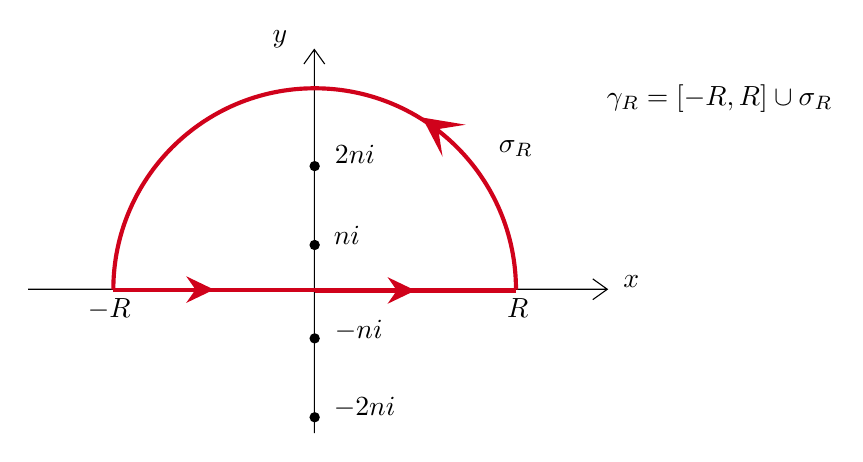
\begin{tikzpicture}[x=0.75pt,y=0.75pt,yscale=-1,xscale=1]
%uncomment if require: \path (0,224); %set diagram left start at 0, and has height of 224

%Shape: Axis 2D [id:dp7020002747782936] 
\draw  (112.5,140.17) -- (391.5,140.17)(250.33,24.63) -- (250.33,209.5) (384.5,135.17) -- (391.5,140.17) -- (384.5,145.17) (245.33,31.63) -- (250.33,24.63) -- (255.33,31.63)  ;
%Straight Lines [id:da8245049527209181] 
\draw [color={rgb, 255:red, 208; green, 2; blue, 27 }  ,draw opacity=1 ][line width=1.5]    (250.5,140.75) -- (347.5,140.75) ;
\draw [shift={(299,140.75)}, rotate = 180] [fill={rgb, 255:red, 208; green, 2; blue, 27 }  ,fill opacity=1 ][line width=0.08]  [draw opacity=0] (13.4,-6.43) -- (0,0) -- (13.4,6.44) -- (8.9,0) -- cycle    ;
%Shape: Arc [id:dp6724290607980123] 
\draw  [draw opacity=0][line width=1.5]  (153.5,140.33) .. controls (153.5,86.76) and (196.93,43.33) .. (250.5,43.33) .. controls (304.07,43.33) and (347.5,86.76) .. (347.5,140.33) -- (250.5,140.33) -- cycle ; \draw  [color={rgb, 255:red, 208; green, 2; blue, 27 }  ,draw opacity=1 ][line width=1.5]  (153.5,140.33) .. controls (153.5,86.76) and (196.93,43.33) .. (250.5,43.33) .. controls (304.07,43.33) and (347.5,86.76) .. (347.5,140.33) ;
%Straight Lines [id:da5477015911612453] 
\draw [color={rgb, 255:red, 208; green, 2; blue, 27 }  ,draw opacity=1 ][line width=1.5]    (153.5,140.33) -- (250.5,140.33) ;
\draw [shift={(202,140.33)}, rotate = 180] [fill={rgb, 255:red, 208; green, 2; blue, 27 }  ,fill opacity=1 ][line width=0.08]  [draw opacity=0] (13.4,-6.43) -- (0,0) -- (13.4,6.44) -- (8.9,0) -- cycle    ;
\draw  [draw opacity=0][fill={rgb, 255:red, 208; green, 2; blue, 27 }  ,fill opacity=1 ] (312.12,76.27) -- (302.31,57.43) -- (323.27,60.88) -- (310,63) -- cycle ;
%Shape: Circle [id:dp3205475558675792] 
\draw  [draw opacity=0][fill={rgb, 255:red, 0; green, 0; blue, 0 }  ,fill opacity=1 ] (248,80.83) .. controls (248,79.45) and (249.12,78.33) .. (250.5,78.33) .. controls (251.88,78.33) and (253,79.45) .. (253,80.83) .. controls (253,82.21) and (251.88,83.33) .. (250.5,83.33) .. controls (249.12,83.33) and (248,82.21) .. (248,80.83) -- cycle ;
%Shape: Circle [id:dp21100228306693403] 
\draw  [draw opacity=0][fill={rgb, 255:red, 0; green, 0; blue, 0 }  ,fill opacity=1 ] (248,118.83) .. controls (248,117.45) and (249.12,116.33) .. (250.5,116.33) .. controls (251.88,116.33) and (253,117.45) .. (253,118.83) .. controls (253,120.21) and (251.88,121.33) .. (250.5,121.33) .. controls (249.12,121.33) and (248,120.21) .. (248,118.83) -- cycle ;
%Shape: Circle [id:dp731209382058088] 
\draw  [draw opacity=0][fill={rgb, 255:red, 0; green, 0; blue, 0 }  ,fill opacity=1 ] (248,163.83) .. controls (248,162.45) and (249.12,161.33) .. (250.5,161.33) .. controls (251.88,161.33) and (253,162.45) .. (253,163.83) .. controls (253,165.21) and (251.88,166.33) .. (250.5,166.33) .. controls (249.12,166.33) and (248,165.21) .. (248,163.83) -- cycle ;
%Shape: Circle [id:dp8736348536667242] 
\draw  [draw opacity=0][fill={rgb, 255:red, 0; green, 0; blue, 0 }  ,fill opacity=1 ] (248,201.83) .. controls (248,200.45) and (249.12,199.33) .. (250.5,199.33) .. controls (251.88,199.33) and (253,200.45) .. (253,201.83) .. controls (253,203.21) and (251.88,204.33) .. (250.5,204.33) .. controls (249.12,204.33) and (248,203.21) .. (248,201.83) -- cycle ;

% Text Node
\draw (342,143.4) node [anchor=north west][inner sep=0.75pt]    {$R$};
% Text Node
\draw (398,132.4) node [anchor=north west][inner sep=0.75pt]    {$x$};
% Text Node
\draw (229,14.4) node [anchor=north west][inner sep=0.75pt]    {$y$};
% Text Node
\draw (140,143.4) node [anchor=north west][inner sep=0.75pt]    {$-R$};
% Text Node
\draw (338,67.4) node [anchor=north west][inner sep=0.75pt]    {$\sigma _{R}$};
% Text Node
\draw (390,40.4) node [anchor=north west][inner sep=0.75pt]    {$\gamma _{R} =[ -R,R] \cup \sigma _{R}$};
% Text Node
\draw (259,69.4) node [anchor=north west][inner sep=0.75pt]    {$2ni$};
% Text Node
\draw (258.5,108.4) node [anchor=north west][inner sep=0.75pt]    {$ni$};
% Text Node
\draw (259,153.9) node [anchor=north west][inner sep=0.75pt]    {$-ni$};
% Text Node
\draw (258.5,190.9) node [anchor=north west][inner sep=0.75pt]    {$-2ni$};


\end{tikzpicture}
\end{figure}
\FloatBarrier
\begin{equation*}
\begin{aligned}
I^{\star }_{n} & =2\pi i\cdotp \{\mathrm{Res}( g_{n} ,2ni) +\mathrm{Res}( g_{n} ,ni)\} =2\pi i\cdotp \left\{-\frac{i}{6n^{3}} +\frac{i}{12n^{3}}\right\}\\
I^{\star }_{n} & =\underbrace{\int _{\sigma _{R}} g( z) dz}_{\xrightarrow{R\rightarrow +\infty } 0} +\underbrace{\int ^{R}_{-R} g( z) dz}_{\xrightarrow{R\rightarrow +\infty } I_{n}}\\
 & \Rightarrow I_{n} =\frac{\pi }{6n^{3}}\\
 & \Rightarrow \Vert f_{n,\alpha } -F_{\alpha }\Vert _{L^{1}} =n^{\alpha } \cdotp \frac{\pi }{6n^{3}}\xrightarrow{n\rightarrow +\infty } 0\ \ \Leftrightarrow \ \ \alpha < 3\land \alpha \in [ 0,4)
\end{aligned}
\end{equation*}

Studiamo ora la norma $L^{\infty }$

Per $\alpha \in [ 0,4)$\begin{equation*}
\begin{aligned}
\Vert f_{n,\alpha } -F_{\alpha }\Vert _{L^{\infty }} & =\Vert f_{n,\alpha }\Vert _{L^{\infty }} & \\
 & =\max_{x\in \mathbb{R}} f_{n,\alpha }( x) & \left( f_{n} \ \text{sono continue e positive}\right)\\
 & =f_{n,\alpha }( 0) & \text{(simmetria)}\\
 & =\frac{1}{4n^{4-\alpha }}\xrightarrow{n\rightarrow +\infty } 0 & \\
 & \Rightarrow \ \ f_{n,\alpha }\xrightarrow[n\rightarrow +\infty ]{L^{\infty }(\mathbb{R})} F_{\alpha } & 
\end{aligned}
\end{equation*}Per $\alpha =4$\begin{equation*}
\begin{aligned}
\Vert f_{n,4} -F_{4}\Vert _{L^{\infty }} & =\left\Vert f_{n,4} -\frac{1}{4}\right\Vert _{L^{\infty }}\\
 & =\max_{x\in \mathbb{R}}\left[\frac{n^{4}}{\left( x^{2} +n^{2}\right)\left( x^{2} +4n^{2}\right)} -\frac{1}{4}\right]\\
 & =\frac{1}{4}\cancel{\xrightarrow{n\rightarrow +\infty }} 0\\
 & \Rightarrow \ \ f_{n,4}\cancel{\xrightarrow[n\rightarrow +\infty ]{L^{\infty }(\mathbb{R})}} F_{4}
\end{aligned}
\end{equation*}
\end{enumerate}
\Soluzione
\begin{theorem}
Sia $f:\mathbb{R}\rightarrow \mathbb{R}$, $T$-periodica, allora la serie di Fourier associata ad $f$ è\begin{equation*}
F( x) =\frac{a_{0}}{2} +\sum\limits ^{\infty }_{n=1}\left[ a_{n}\cos\left(\frac{2\pi n}{T} x\right) +b_{n}\sin\left(\frac{2\pi n}{T} x\right)\right]
\end{equation*}

dove
\begin{gather*}
a_{0} =\frac{2}{T}\int ^{\frac{T}{2}}_{-\frac{T}{2}} f( x) dx\\
a_{n} =\frac{2}{T}\int ^{\frac{T}{2}}_{-\frac{T}{2}} f( x)\cos\left(\frac{2\pi n}{T} x\right) dx\ \ \ \ b_{n} =\frac{2}{T}\int ^{\frac{T}{2}}_{-\frac{T}{2}} f( x)\sin\left(\frac{2\pi n}{T} x\right) dx
\end{gather*}
\textbf{NB.} Se $f$ è pari, il seno è dispari, $P\cdotp D=D\Rightarrow b_{n} =0\ \forall n\geqslant 1$.

\textbf{NB.} Se $f$ è dispari, il coseno è pari, $D\cdotp P=D\Rightarrow a_{n} =0\ \forall n\geqslant 0$.
\end{theorem}
\begin{enumerate}
\item Disegnamo la funzione

\begin{figure}[htpb]
	\centering
\tikzset{every picture/.style={line width=0.75pt}} %set default line width to 0.75pt        

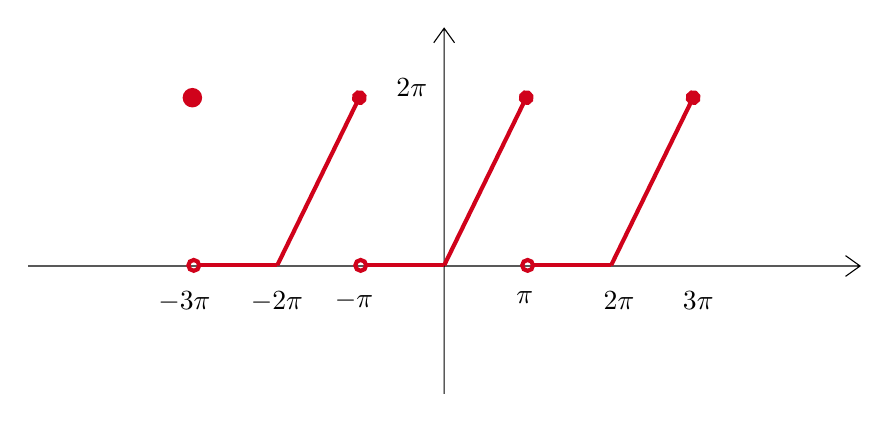
\begin{tikzpicture}[x=0.75pt,y=0.75pt,yscale=-1,xscale=1]
%uncomment if require: \path (0,198); %set diagram left start at 0, and has height of 198

%Shape: Axis 2D [id:dp24320808205526556] 
\draw  (100.11,120.97) -- (500.89,120.97)(300.5,6.41) -- (300.5,182.63) (493.89,115.97) -- (500.89,120.97) -- (493.89,125.97) (295.5,13.41) -- (300.5,6.41) -- (305.5,13.41)  ;
%Straight Lines [id:da6107470839046387] 
\draw [color={rgb, 255:red, 208; green, 2; blue, 27 }  ,draw opacity=1 ][line width=1.5]    (300.5,120.67) -- (340.04,39.87) ;
\draw [shift={(340.04,39.87)}, rotate = 296.08] [color={rgb, 255:red, 208; green, 2; blue, 27 }  ,draw opacity=1 ][fill={rgb, 255:red, 208; green, 2; blue, 27 }  ,fill opacity=1 ][line width=1.5]      (0, 0) circle [x radius= 2.61, y radius= 2.61]   ;
%Straight Lines [id:da4254536093640342] 
\draw [color={rgb, 255:red, 208; green, 2; blue, 27 }  ,draw opacity=1 ][line width=1.5]    (300.5,120.67) -- (261.9,120.67) ;
\draw [shift={(260.29,120.67)}, rotate = 180] [color={rgb, 255:red, 208; green, 2; blue, 27 }  ,draw opacity=1 ][line width=1.5]      (0, 0) circle [x radius= 2.61, y radius= 2.61]   ;

%Straight Lines [id:da07742835835652251] 
\draw [color={rgb, 255:red, 208; green, 2; blue, 27 }  ,draw opacity=1 ][line width=1.5]    (380.92,120.67) -- (420.46,39.87) ;
\draw [shift={(420.46,39.87)}, rotate = 296.08] [color={rgb, 255:red, 208; green, 2; blue, 27 }  ,draw opacity=1 ][fill={rgb, 255:red, 208; green, 2; blue, 27 }  ,fill opacity=1 ][line width=1.5]      (0, 0) circle [x radius= 2.61, y radius= 2.61]   ;
%Straight Lines [id:da9261529019653281] 
\draw [color={rgb, 255:red, 208; green, 2; blue, 27 }  ,draw opacity=1 ][line width=1.5]    (380.92,120.67) -- (342.32,120.67) ;
\draw [shift={(340.71,120.67)}, rotate = 180] [color={rgb, 255:red, 208; green, 2; blue, 27 }  ,draw opacity=1 ][line width=1.5]      (0, 0) circle [x radius= 2.61, y radius= 2.61]   ;

%Straight Lines [id:da5018794931536248] 
\draw [color={rgb, 255:red, 208; green, 2; blue, 27 }  ,draw opacity=1 ][line width=1.5]    (220.08,120.67) -- (259.62,39.87) ;
\draw [shift={(259.62,39.87)}, rotate = 296.08] [color={rgb, 255:red, 208; green, 2; blue, 27 }  ,draw opacity=1 ][fill={rgb, 255:red, 208; green, 2; blue, 27 }  ,fill opacity=1 ][line width=1.5]      (0, 0) circle [x radius= 2.61, y radius= 2.61]   ;
%Straight Lines [id:da10630889376486596] 
\draw [color={rgb, 255:red, 208; green, 2; blue, 27 }  ,draw opacity=1 ][line width=1.5]    (220.08,120.67) -- (181.48,120.67) ;
\draw [shift={(179.87,120.67)}, rotate = 180] [color={rgb, 255:red, 208; green, 2; blue, 27 }  ,draw opacity=1 ][line width=1.5]      (0, 0) circle [x radius= 2.61, y radius= 2.61]   ;

%Shape: Ellipse [id:dp5794600318678271] 
\draw  [draw opacity=0][fill={rgb, 255:red, 208; green, 2; blue, 27 }  ,fill opacity=1 ] (174.5,39.87) .. controls (174.5,37.28) and (176.6,35.18) .. (179.2,35.18) .. controls (181.79,35.18) and (183.89,37.28) .. (183.89,39.87) .. controls (183.89,42.46) and (181.79,44.57) .. (179.2,44.57) .. controls (176.6,44.57) and (174.5,42.46) .. (174.5,39.87) -- cycle ;

% Text Node
\draw (161.5,132.13) node [anchor=north west][inner sep=0.75pt]  [font=\normalsize]  {$-3\pi $};
% Text Node
\draw (206.07,132.13) node [anchor=north west][inner sep=0.75pt]  [font=\normalsize]  {$-2\pi $};
% Text Node
\draw (246.6,132.13) node [anchor=north west][inner sep=0.75pt]  [font=\normalsize]  {$-\pi $};
% Text Node
\draw (334.04,132.13) node [anchor=north west][inner sep=0.75pt]  [font=\normalsize]  {$\pi $};
% Text Node
\draw (376.1,132.13) node [anchor=north west][inner sep=0.75pt]  [font=\normalsize]  {$2\pi $};
% Text Node
\draw (414.3,132.13) node [anchor=north west][inner sep=0.75pt]  [font=\normalsize]  {$3\pi $};
% Text Node
\draw (276.25,29.26) node [anchor=north west][inner sep=0.75pt]  [font=\normalsize]  {$2\pi $};


\end{tikzpicture}
\end{figure}
\FloatBarrier

\item $f$ è regolare a tratti in $[ -\pi ,\pi ] \Rightarrow $ la serie di Fourier $F( x)$ converge puntualmente $\forall x\in \mathbb{R}$.
\begin{enumerate}
\item se $x$ è un punto di continuità, $F( x)$ converge a $f( x)$
\item se $x$ non è punto di continuità, $F( x)$ converge alla media tra il limite destro e sinistro
\end{enumerate}

nel nostro caso $f$ è continua in ogni punto $x\neq ( 2k+1) \pi ,k\in \mathbb{Z}$ e presenta delle discontinuità di I specie (tipo salto) nei punti $x=( 2k+1) \pi ,k\in \mathbb{Z}$.
\begin{enumerate}
\item $F( x)$ converge puntualmente a\begin{equation*}
f( x) \ \ \ \ \forall x\neq ( 2k+1) \pi ,k\in \mathbb{Z}
\end{equation*}
\item $F( x)$ converge puntualmente a\begin{equation*}
\frac{f\left( x^{+}\right) +f\left( x^{-}\right)}{2} =\frac{0+2\pi }{2} =\pi \ \ \ \ \forall x=( 2k+1) \pi ,k\in \mathbb{Z}
\end{equation*}
\end{enumerate}
\item Calcoliamo i coefficienti\begin{align*}
a_{0} & =\frac{2}{2\pi }\int ^{\pi }_{-\pi } f( x) dx=\frac{1}{\pi }\left\{\int ^{0}_{-\pi } f( x) dx+\int ^{\pi }_{0} f( x) dx\right\}\\
 & =\frac{1}{\pi }\int ^{\pi }_{0} f( x) dx=\frac{1}{\pi }\int ^{\pi }_{0} 2xdx=\frac{1}{\pi }\left[ x^{2}\right]^{\pi }_{0} =\frac{1}{\pi } \pi ^{2} =\textcolor[rgb]{0.82,0.01,0.11}{\pi }\\
 & \\
a_{n} & \overset{n\geqslant 1}{=}\frac{1}{\pi }\int ^{\pi }_{-\pi } f( x)\cos( nx) dx=\frac{1}{\pi }\int ^{\pi }_{0} 2x\cos( nx) dx\\
 & \\
 & \begin{array}{ l l }
h( x) =2x & h'( x) =2\\
g( x) =\frac{1}{n}\sin( nx) & g'( x) =\cos( nx)
\end{array}\\
 & \\
 & \overset{\text{ipp}}{=}\frac{1}{\pi }\left\{\left[\frac{2x}{n}\sin( nx)\right]^{\pi }_{0} -\int ^{\pi }_{0}\frac{2}{n}\sin( nx) dx\right\}\\
 & =\frac{1}{\pi }\left\{\cancel{\frac{2\pi }{n}\sin( n\pi )} -0+\left[\frac{2\cos( nx)}{n^{2}}\right]^{\pi }_{0}\right\}\\
 & =\frac{1}{\pi }\left\{\frac{2\cos( n\pi )}{n^{2}} -\frac{2}{n^{2}}\right\} =\frac{1}{\pi }\left\{\frac{2( -1)^{n}}{n^{2}} -\frac{2}{n^{2}}\right\}\\
 & =\textcolor[rgb]{0.82,0.01,0.11}{\frac{2}{\pi }}\textcolor[rgb]{0.82,0.01,0.11}{\frac{( -1)^{n} -1}{n^{2}}}\\
 & \\
b_{n} & =\frac{1}{\pi }\int ^{\pi }_{-\pi } f( x)\sin( nx) dx=\frac{1}{\pi }\int ^{\pi }_{0} 2x\sin( nx) dx\\
 & \\
 & \begin{array}{ l l }
k( x) =2x & k'( x) =2\\
r( x) =-\frac{1}{n}\cos( nx) & r'( x) =\sin( nx)
\end{array}\\
 & \\
 & \overset{\text{ipp}}{=}\frac{1}{\pi }\left\{\left[ -\frac{2x}{n}\cos( nx)\right]^{\pi }_{0} +\int ^{\pi }_{0}\frac{2}{n}\cos( nx) dx\right\}\\
 & =\frac{1}{\pi }\left\{-\frac{2\pi }{n}\cos( n\pi ) +0+\left[\frac{2\sin( nx)}{n^{2}}\right]^{\pi }_{0}\right\}\\
 & =\frac{1}{\pi }\left\{-\frac{2\pi }{n}( -1)^{n}\right\} =\textcolor[rgb]{0.82,0.01,0.11}{\frac{2}{n}}\textcolor[rgb]{0.82,0.01,0.11}{(}\textcolor[rgb]{0.82,0.01,0.11}{-1}\textcolor[rgb]{0.82,0.01,0.11}{)}\textcolor[rgb]{0.82,0.01,0.11}{^{n+1}}
\end{align*}

La serie di Fourier di $f$ è\begin{equation*}
F( x) =\frac{\pi }{2} +2\sum\limits ^{\infty }_{n=1}\left[\frac{( -1)^{n} -1}{\pi n^{2}}\cos( nx) +\frac{( -1)^{n+1}}{n}\sin( nx)\right]
\end{equation*}
\item Poiché $f\in L^{2}([ -\pi ,\pi ])$\begin{equation*}
\int ^{\pi }_{-\pi }| f( x)| ^{2} dx=\int ^{\pi }_{0}( 2x)^{2} dx=\int ^{\pi }_{0} 4x^{2} dx=\frac{4}{3} \pi ^{3} < +\infty 
\end{equation*}

allora $F( x)$ di $f$ converge in media quadratica.
\item Poiché $f$ \underline{\textbf{non}} è continua, allora la convergenza \underline{\textbf{non}} è uniforme su $\mathbb{R}$.
\end{enumerate}
\Soluzione
\begin{enumerate}
\item $f$ è pari $\Rightarrow b_{n} =0\ \forall n\in \mathbb{N}$\begin{equation*}
a_{k} =\frac{2}{\pi }\int ^{\frac{\pi }{2}}_{-\frac{\pi }{2}}\cos\left(\sqrt{2} x\right)\cos( 2kx) dx\ \ \forall k\in \mathbb{N}
\end{equation*}

modo $A$: calcolo per parti e ottengo un integrale ciclico.

modo $B$: usare la formula di Werner, usiamo questo\begin{equation*}
\cos \alpha \cos \beta =\frac{1}{2}[\cos( \alpha +\beta ) +\cos( \alpha -\beta )]
\end{equation*}

Procediamo al calcolo\begin{align*}
a_{k} & =\frac{\cancel{2}}{\pi }\int ^{\frac{\pi }{2}}_{-\frac{\pi }{2}}\frac{1}{\cancel{2}}\left\{\cos\left(\sqrt{2} x+2kx\right) +\cos\left(\sqrt{2} x-2kx\right)\right\} dx\\
 & =\frac{1}{\pi }\int ^{\frac{\pi }{2}}_{-\frac{\pi }{2}}\left\{\cos\left(\left(\sqrt{2} +2k\right) x\right) +\cos\left(\left(\sqrt{2} -2k\right) x\right)\right\} dx\\
 & =\frac{1}{\pi }\left\{\left[\frac{\sin\left(\left(\sqrt{2} +2k\right) x\right)}{\sqrt{2} +2k}\right]^{\frac{\pi }{2}}_{-\frac{\pi }{2}} +\left[\frac{\sin\left(\left(\sqrt{2} -2k\right) x\right)}{\sqrt{2} -2k}\right]^{\frac{\pi }{2}}_{-\frac{\pi }{2}}\right\}\\
 & =\frac{1}{\pi }\left\{\frac{\sin\left(\frac{\pi }{\sqrt{2}} +k\pi \right)}{\sqrt{2} +2k} +\frac{\sin\left(\frac{\pi }{\sqrt{2}} +k\pi \right)}{\sqrt{2} +2k} +\left[\frac{\sin\left(\left(\sqrt{2} -2k\right) x\right)}{\sqrt{2} -2k}\right]^{\frac{\pi }{2}}_{-\frac{\pi }{2}}\right\}\\
 & =\frac{1}{\pi }\left\{\frac{2\sin\left(\frac{\pi }{\sqrt{2}} +k\pi \right)}{\sqrt{2} +2k} +\frac{2\sin\left(\frac{\pi }{\sqrt{2}} -k\pi \right)}{\sqrt{2} -2k}\right\}\\
 & =\frac{2( -1)^{k}\sin\left(\frac{\pi }{\sqrt{2}}\right)}{\pi }\left(\frac{1}{\sqrt{2} +2k} +\frac{1}{\sqrt{2} -2k}\right)\\
 & =\frac{2( -1)^{k}\sin\left(\frac{\pi }{\sqrt{2}}\right)}{\pi }\left(\frac{1}{2k+\sqrt{2}} -\frac{1}{2k-\sqrt{2}}\right)\\
 & =-\frac{2\sqrt{2}( -1)^{k}\sin\left(\frac{\pi }{\sqrt{2}}\right)}{\pi \left( 2k^{2} -1\right)}
\end{align*}
\item La serie di Fourier di $f$ è\begin{equation*}
F( x) =\frac{a_{0}}{2} +\sum\limits ^{\infty }_{k=1} a_{k}\cos( 2kx)
\end{equation*}

per $x=\frac{\pi }{2}$\begin{equation*}
\begin{aligned}
F\left(\frac{\pi }{2}\right) & =\cos\left(\sqrt{2} \cdotp \frac{\pi }{2}\right) =\textcolor[rgb]{0.25,0.46,0.02}{\cos\left(\frac{\pi }{\sqrt{2}}\right)}\\
F\left(\frac{\pi }{2}\right) & =\frac{\sqrt{2}}{\pi }\sin\left(\frac{\pi }{\sqrt{2}}\right) +\sum\limits ^{\infty }_{k=1} a_{k}( -1)^{k}\\
 & =\textcolor[rgb]{0.74,0.06,0.88}{\frac{\sqrt{2}}{\pi }\sin\left(\frac{\pi }{\sqrt{2}}\right)}\textcolor[rgb]{0.96,0.65,0.14}{-\frac{2\sqrt{2}\sin\left(\frac{\pi }{\sqrt{2}}\right)}{\pi }}\sum\limits ^{\infty }_{k=1}\frac{( -1)^{k}( -1)^{k}}{\left( 2k^{2} -1\right)}\\
 & \\
\Rightarrow \ \ \sum\limits ^{\infty }_{k=1}\frac{1}{\left( 2k^{2} -1\right)} & =\frac{\textcolor[rgb]{0.25,0.46,0.02}{\cos\left(\frac{\pi }{\sqrt{2}}\right)} -\textcolor[rgb]{0.74,0.06,0.88}{\frac{\sqrt{2}}{\pi }\sin\left(\frac{\pi }{\sqrt{2}}\right)}}{\textcolor[rgb]{0.96,0.65,0.14}{-\frac{2\sqrt{2}\sin\left(\frac{\pi }{\sqrt{2}}\right)}{\pi }}} =-\frac{\textcolor[rgb]{0.25,0.46,0.02}{\cos\left(\frac{\pi }{\sqrt{2}}\right)}}{\textcolor[rgb]{0.96,0.65,0.14}{\frac{2\sqrt{2}\sin\left(\frac{\pi }{\sqrt{2}}\right)}{\pi }}} +\frac{\textcolor[rgb]{0.74,0.06,0.88}{\frac{\sqrt{2}}{\pi }\sin\left(\frac{\pi }{\sqrt{2}}\right)}}{\textcolor[rgb]{0.96,0.65,0.14}{\frac{2\sqrt{2}\sin\left(\frac{\pi }{\sqrt{2}}\right)}{\pi }}}\\
 & =-\frac{\pi }{2\sqrt{2}}\cot\left(\frac{\pi }{\sqrt{2}}\right) +\frac{1}{2}
\end{aligned}
\end{equation*}
\item $f\in L^{2}\left(\left[ -\frac{\pi }{2} ,\frac{\pi }{2}\right]\right) \Rightarrow $ ho convergenza in media quadratica

Criterio di Weierstrass, prendo il termine generale in modulo\begin{gather*}
| a_{k}\cos( 2k\pi )| \leqslant \frac{2\sqrt{2}}{\pi \left( 2k^{2} -1\right)}\\
\sum\limits ^{\infty }_{k=1}\frac{2\sqrt{2}}{\pi \left( 2k^{2} -1\right)} < +\infty \ \ \Rightarrow \ \ \text{convergenza è uniforme su} \ \mathbb{R}
\end{gather*}
\end{enumerate}
\chapter{Esercitazione 6 - Boella}
\ParteEsercizi
\Esercizio{}

Data una funzione $2\pi $-periodica
\begin{equation*}
f:[ -\pi ,\pi ]\rightarrow \mathbb{R} \ \ \ \ f(x)=x^{2}
\end{equation*}
Determinare la sue serie di Fourier. Si riesce a ricondurre la serie ad una nota?
\Esercizio{}

Data una funzione $3$-periodica
\begin{equation*}
f(x)=\begin{cases}
0, & 0\leq x< 1\\
1, & 1\leq x< 2\\
2, & 2\leq x< 3
\end{cases}
\end{equation*}
Determinare la sue serie di Fourier. Si riesce a ricondurre la serie ad una nota?
\Esercizio{}
\begin{definition}
[Spazio delle funzioni test] $\varphi \in D( A)$ se $\varphi \in C^{\infty }( A)$, $\exists K$ compatto tale per cui $\varphi ( x) =0,\forall x\notin K$
\end{definition}
\textit{Esempio.}
\begin{equation*}
\varphi ( x) =\begin{cases}
e^{-\frac{1}{1-x^{2}}} , & | x| < 1\\
0, & | x| \geqslant 1
\end{cases}
\end{equation*}
\fg{0.7}{11-3-1}
\begin{definition}
[Distribuzione] Si chiamano distribuzioni gli oggetti $T\in D'( A)$. $T$ è un funzionale lineare continuo su $D( A)$. Quindi so dire cosa fa $T$ a una funzione test $\varphi $ tramite il prodotto di dualità
\begin{equation*}
T( \varphi ) =\langle T,\varphi \rangle 
\end{equation*}
\end{definition}
\begin{definition}
[Convergenza di funzioni test] Diciamo che $\varphi _{k}\xrightarrow{D( A)} \varphi $ se $\forall \alpha ,D^{\alpha } \varphi _{k}\rightarrow D^{\alpha } \varphi $.
\end{definition}
\begin{definition}
[Prodotto di dualità] Data $T\in D'( A)$, se $T\in L^{1}_{\mathrm{loc}}( A) \Rightarrow \langle T,\varphi \rangle =\int _{A} T( x) \varphi ( x) dx$. Se invece $T\notin L^{1}_{\mathrm{loc}} \Rightarrow \langle T,\varphi \rangle $ lo dobbiamo definire manualmente, per esempio la Delta di Dirac che è definita come
\begin{equation*}
\langle \delta ,\varphi \rangle =\varphi ( 0)
\end{equation*}
Possiamo anche traslarla
\begin{equation*}
\langle \delta _{x_{0}} ,\varphi \rangle =\varphi ( x_{0})
\end{equation*}
\end{definition}
\begin{definition}
[Convergenza di distribuzioni] Diciamo che $T_{n}\xrightarrow{D'( A)} T$ se $\langle T_{n} ,\varphi \rangle \rightarrow \langle T,\varphi \rangle $, $\forall \varphi \in D( A)$.
\end{definition}
Studiare la convergenza in distribuzione della seguente successione
\begin{equation*}
f_{n} (x)=ne^{-n|x|}
\end{equation*}
\Esercizio{}

Studiare la convergenza in distribuzione della seguente successione
\begin{equation*}
f_{n} (x)=\begin{cases}
-3n, & |x|\leq \frac{1}{n}\\
2n, & \frac{1}{n} < |x|\leq \frac{2}{n}\\
0, & |x| >\frac{2}{n}
\end{cases}
\end{equation*}
\Esercizio{}

Studiare la convergenza in distribuzione della seguente successione
\begin{equation*}
f_{n} (x)=nx^{n} \chi _{(0,1)} (x)
\end{equation*}
\ParteSoluzioni
\Soluzione

Osserviamo che la funzione $f(x)=x^{2}$ converge in $L^{2}$ e puntualmente su $\mathbb{R}$.

Osserviamo che $b_{n} =0,\forall n$ perché la funzione è pari.

Calcoliamo ora $a_{0}$ e $a_{n}$:
\begin{align*}
a_{0} & =\frac{1}{\pi }\int ^{\pi }_{-\pi } f(x)dx=\frac{2}{\pi }\int ^{\pi }_{0} f(x)dx=\frac{2}{3} \pi ^{2}\\
 & \\
a_{n} & =\frac{1}{\pi }\int ^{\pi }_{-\pi } f(x)\cos( nx) dx\\
 & =\frac{2}{\pi }\int ^{\pi }_{0} f(x)\cos (nx)dx\\
 & =\frac{2}{\pi }\int ^{\pi }_{0} x^{2}\cos (nx)dx\\
 & \overset{\text{ipp}}{=}\frac{2}{\pi }\left\{\cancel{\left[ x^{2}\frac{\sin (nx)}{n}\right]^{\pi }_{0}} -\frac{2}{n}\int ^{\pi }_{0} x\sin (nx)dx\right\}\\
 & \overset{\text{ipp}}{=} -\frac{4}{n\pi }\left\{\left[ -\frac{x}{n}\cos( nx)\right]^{\pi }_{0} +\cancel{\frac{1}{n}\int ^{\pi }_{0}\cos( nx) dx}\right\}\\
 & =\frac{4}{n\pi } \cdotp \frac{\pi }{n}\cos( n\pi ) =\frac{4}{n^{2}}( -1)^{n}
\end{align*}
La serie di Fourier cercata è:
\begin{equation*}
f(x)=\frac{\pi ^{2}}{3} +\sum ^{\infty }_{n=1} (-1)^{n}\frac{4}{n^{2}}\cos (nx)
\end{equation*}
Inoltre
\begin{equation*}
\sum ^{\infty }_{n=1}( |a_{n} |+|b_{n} |) < \infty \ \ \Rightarrow \ \ \text{c'è anche convergenza uniforme}
\end{equation*}
Ricaviamo alcune serie notevoli.
\begin{itemize}
\item in $x=\pi $\begin{gather*}
\pi ^{2} =f( \pi ) =\frac{\pi ^{2}}{3} +\sum ^{\infty }_{n=1} (-1)^{n}\frac{4}{n^{2}}\cos (n\pi )=\frac{\pi ^{2}}{3} +4\sum ^{\infty }_{n=1}\frac{1}{n^{2}}\\
\Rightarrow \ \ \boxed{\sum ^{\infty }_{n=1}\frac{1}{n^{2}} =\frac{\pi ^{2}}{6}}
\end{gather*}
\item in $x=0$\begin{gather*}
0=f( 0) =\frac{\pi ^{2}}{3} +\sum ^{\infty }_{n=1} (-1)^{n}\frac{4}{n^{2}}\cos (0)=\frac{\pi ^{2}}{3} +4\sum ^{\infty }_{n=1}\frac{(-1)^{n}}{n^{2}}\\
\Rightarrow \ \ \boxed{\sum ^{\infty }_{n=1}\frac{(-1)^{n}}{n^{2}} =-\frac{\pi ^{2}}{12}}
\end{gather*}
\item Parseval\begin{equation*}
\int ^{2\pi }_{0}[ f(x)]^{2} dx=\pi \left[\frac{a^{2}_{0}}{2} +\sum ^{\infty }_{n=1} (a^{2}_{n} +b^{2}_{n} )\right]
\end{equation*}

Allora\begin{equation*}
\begin{aligned}
\int ^{\pi }_{-\pi }\left( x^{2}\right)^{2} dx & =\pi \left[\frac{\left(\frac{2}{3} \pi ^{2}\right)^{2}}{2} +\sum\limits ^{\infty }_{n=1}\frac{16}{n^{4}}\right]\\
2\cdotp \frac{\pi ^{5}}{5} & =\pi \left[\frac{2}{9} \pi ^{4} +16\sum\limits ^{\infty }_{n=1}\frac{1}{n^{4}}\right]\\
\left(\frac{2}{5} -\frac{2}{9}\right) \pi ^{4} & =16\sum\limits ^{\infty }_{n=1}\frac{1}{n^{4}} \ \ \Rightarrow \ \ \boxed{\sum\limits ^{\infty }_{n=1}\frac{1}{n^{4}} =\frac{\pi ^{4}}{90}}
\end{aligned}
\end{equation*}
\end{itemize}
\Soluzione

Iniziamo osservando che la funzione
\begin{equation*}
f(x)=\begin{cases}
0, & 0\leq x< 1\\
1, & 1\leq x< 2\\
2, & 2\leq x< 3
\end{cases}
\end{equation*}
converge in $L^{2}( 0,3)$. Converge inoltre puntualmente q.o. su $\mathbb{R}$ (a meno dell'insieme $x\notin \mathbb{Z}$).


\begin{figure}[htpb]
	\centering
\tikzset{every picture/.style={line width=0.75pt}} %set default line width to 0.75pt        

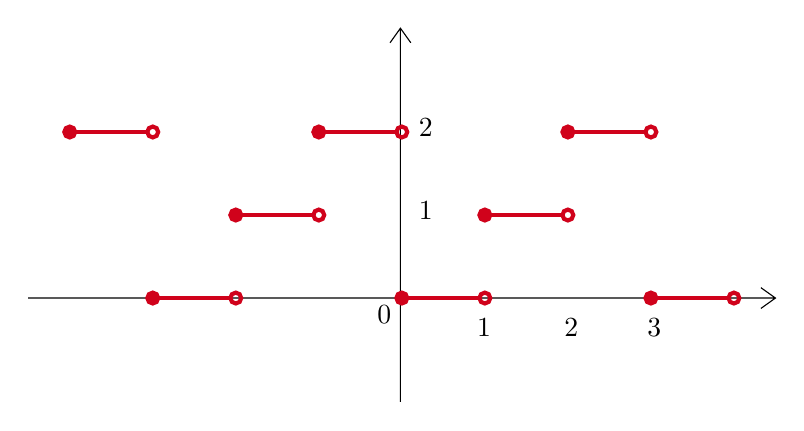
\begin{tikzpicture}[x=0.75pt,y=0.75pt,yscale=-1,xscale=1]
%uncomment if require: \path (0,214); %set diagram left start at 0, and has height of 214

%Shape: Axis 2D [id:dp9173052200245366] 
\draw  (120,150) -- (480,150)(299.33,20) -- (299.33,200) (473,145) -- (480,150) -- (473,155) (294.33,27) -- (299.33,20) -- (304.33,27)  ;
%Straight Lines [id:da6842800458327545] 
\draw [color={rgb, 255:red, 208; green, 2; blue, 27 }  ,draw opacity=1 ][line width=1.5]    (300,150) -- (338.39,150) ;
\draw [shift={(340,150)}, rotate = 0] [color={rgb, 255:red, 208; green, 2; blue, 27 }  ,draw opacity=1 ][line width=1.5]      (0, 0) circle [x radius= 2.61, y radius= 2.61]   ;
\draw [shift={(300,150)}, rotate = 0] [color={rgb, 255:red, 208; green, 2; blue, 27 }  ,draw opacity=1 ][fill={rgb, 255:red, 208; green, 2; blue, 27 }  ,fill opacity=1 ][line width=1.5]      (0, 0) circle [x radius= 2.61, y radius= 2.61]   ;
%Straight Lines [id:da3441135935225803] 
\draw [color={rgb, 255:red, 208; green, 2; blue, 27 }  ,draw opacity=1 ][line width=1.5]    (340,110) -- (378.39,110) ;
\draw [shift={(380,110)}, rotate = 0] [color={rgb, 255:red, 208; green, 2; blue, 27 }  ,draw opacity=1 ][line width=1.5]      (0, 0) circle [x radius= 2.61, y radius= 2.61]   ;
\draw [shift={(340,110)}, rotate = 0] [color={rgb, 255:red, 208; green, 2; blue, 27 }  ,draw opacity=1 ][fill={rgb, 255:red, 208; green, 2; blue, 27 }  ,fill opacity=1 ][line width=1.5]      (0, 0) circle [x radius= 2.61, y radius= 2.61]   ;
%Straight Lines [id:da03802847326309822] 
\draw [color={rgb, 255:red, 208; green, 2; blue, 27 }  ,draw opacity=1 ][line width=1.5]    (380,70) -- (418.39,70) ;
\draw [shift={(420,70)}, rotate = 0] [color={rgb, 255:red, 208; green, 2; blue, 27 }  ,draw opacity=1 ][line width=1.5]      (0, 0) circle [x radius= 2.61, y radius= 2.61]   ;
\draw [shift={(380,70)}, rotate = 0] [color={rgb, 255:red, 208; green, 2; blue, 27 }  ,draw opacity=1 ][fill={rgb, 255:red, 208; green, 2; blue, 27 }  ,fill opacity=1 ][line width=1.5]      (0, 0) circle [x radius= 2.61, y radius= 2.61]   ;
%Straight Lines [id:da9565199441833196] 
\draw [color={rgb, 255:red, 208; green, 2; blue, 27 }  ,draw opacity=1 ][line width=1.5]    (180,150) -- (218.39,150) ;
\draw [shift={(220,150)}, rotate = 0] [color={rgb, 255:red, 208; green, 2; blue, 27 }  ,draw opacity=1 ][line width=1.5]      (0, 0) circle [x radius= 2.61, y radius= 2.61]   ;
\draw [shift={(180,150)}, rotate = 0] [color={rgb, 255:red, 208; green, 2; blue, 27 }  ,draw opacity=1 ][fill={rgb, 255:red, 208; green, 2; blue, 27 }  ,fill opacity=1 ][line width=1.5]      (0, 0) circle [x radius= 2.61, y radius= 2.61]   ;
%Straight Lines [id:da9765401043379787] 
\draw [color={rgb, 255:red, 208; green, 2; blue, 27 }  ,draw opacity=1 ][line width=1.5]    (220,110) -- (258.39,110) ;
\draw [shift={(260,110)}, rotate = 0] [color={rgb, 255:red, 208; green, 2; blue, 27 }  ,draw opacity=1 ][line width=1.5]      (0, 0) circle [x radius= 2.61, y radius= 2.61]   ;
\draw [shift={(220,110)}, rotate = 0] [color={rgb, 255:red, 208; green, 2; blue, 27 }  ,draw opacity=1 ][fill={rgb, 255:red, 208; green, 2; blue, 27 }  ,fill opacity=1 ][line width=1.5]      (0, 0) circle [x radius= 2.61, y radius= 2.61]   ;
%Straight Lines [id:da7209581982756688] 
\draw [color={rgb, 255:red, 208; green, 2; blue, 27 }  ,draw opacity=1 ][line width=1.5]    (260,70) -- (298.39,70) ;
\draw [shift={(300,70)}, rotate = 0] [color={rgb, 255:red, 208; green, 2; blue, 27 }  ,draw opacity=1 ][line width=1.5]      (0, 0) circle [x radius= 2.61, y radius= 2.61]   ;
\draw [shift={(260,70)}, rotate = 0] [color={rgb, 255:red, 208; green, 2; blue, 27 }  ,draw opacity=1 ][fill={rgb, 255:red, 208; green, 2; blue, 27 }  ,fill opacity=1 ][line width=1.5]      (0, 0) circle [x radius= 2.61, y radius= 2.61]   ;
%Straight Lines [id:da15781035361747886] 
\draw [color={rgb, 255:red, 208; green, 2; blue, 27 }  ,draw opacity=1 ][line width=1.5]    (140,70) -- (178.39,70) ;
\draw [shift={(180,70)}, rotate = 0] [color={rgb, 255:red, 208; green, 2; blue, 27 }  ,draw opacity=1 ][line width=1.5]      (0, 0) circle [x radius= 2.61, y radius= 2.61]   ;
\draw [shift={(140,70)}, rotate = 0] [color={rgb, 255:red, 208; green, 2; blue, 27 }  ,draw opacity=1 ][fill={rgb, 255:red, 208; green, 2; blue, 27 }  ,fill opacity=1 ][line width=1.5]      (0, 0) circle [x radius= 2.61, y radius= 2.61]   ;
%Straight Lines [id:da6022039956275556] 
\draw [color={rgb, 255:red, 208; green, 2; blue, 27 }  ,draw opacity=1 ][line width=1.5]    (420,150) -- (458.39,150) ;
\draw [shift={(460,150)}, rotate = 0] [color={rgb, 255:red, 208; green, 2; blue, 27 }  ,draw opacity=1 ][line width=1.5]      (0, 0) circle [x radius= 2.61, y radius= 2.61]   ;
\draw [shift={(420,150)}, rotate = 0] [color={rgb, 255:red, 208; green, 2; blue, 27 }  ,draw opacity=1 ][fill={rgb, 255:red, 208; green, 2; blue, 27 }  ,fill opacity=1 ][line width=1.5]      (0, 0) circle [x radius= 2.61, y radius= 2.61]   ;

% Text Node
\draw (335,158.9) node [anchor=north west][inner sep=0.75pt]    {$1$};
% Text Node
\draw (377,158.9) node [anchor=north west][inner sep=0.75pt]    {$2$};
% Text Node
\draw (417,158.9) node [anchor=north west][inner sep=0.75pt]    {$3$};
% Text Node
\draw (307,102.4) node [anchor=north west][inner sep=0.75pt]    {$1$};
% Text Node
\draw (307,62.4) node [anchor=north west][inner sep=0.75pt]    {$2$};
% Text Node
\draw (287,152.4) node [anchor=north west][inner sep=0.75pt]    {$0$};


\end{tikzpicture}
\end{figure}
\FloatBarrier

\begin{equation*}
f( x) \sim \frac{a_{0}}{2} +\sum\limits ^{\infty }_{n=1}\left[ a_{n}\cos\left(\frac{2n\pi }{3} x\right) +b_{n}\sin\left(\frac{2n\pi }{3} x\right)\right]
\end{equation*}
Calcoliamo ora i coefficienti:
\begin{align*}
a_{0} & =\frac{1}{3/2}\int ^{3}_{0} f(x)dx=\frac{2}{3} \cdotp 3=2\\
 & \\
a_{n} & =\frac{1}{3/2}\int ^{3}_{0} f(x)\cos\left(\frac{2n\pi }{3}\right) dx=\frac{2}{3}\left\{\int ^{2}_{1} 1\cos\left(\frac{2n\pi }{3}\right) dx+\int ^{3}_{2} 2\cos\left(\frac{2n\pi }{3}\right) dx\right\}\\
 & =\frac{2}{3}\left\{\left[\frac{3}{2n\pi }\sin\left(\frac{2n\pi }{3} x\right)\right]^{2}_{1} +2\left[\frac{3}{2n\pi }\sin\left(\frac{2n\pi }{3} x\right)\right]^{3}_{2}\right\}\\
 & =\frac{2}{3}\frac{3}{2n\pi }\left\{\sin\left(\frac{4n\pi }{3}\right) -\sin\left(\frac{2n\pi }{3}\right) +\cancel{2\sin( 2n\pi )} -2\sin\left(\frac{4n\pi }{3}\right)\right\} =0,\ \forall n\\
 & \\
b_{n} & =\frac{2}{3}\int ^{3}_{0} f(x)\sin\left(\frac{2n\pi }{3}\right) dx=\frac{2}{3}\left\{\int ^{2}_{1} 1\sin\left(\frac{2n\pi }{3}\right) dx+\int ^{3}_{2} 2\sin\left(\frac{2n\pi }{3}\right) dx\right\}\\
 & =\frac{2}{3}\frac{3}{2n\pi }\left\{\left[ -\cos\left(\frac{2n\pi }{3}\right)\right]^{2}_{1} -2\left[\cos\left(\frac{2n\pi }{3}\right)\right]^{3}_{2}\right\}\\
 & =-\frac{1}{n\pi }\left\{\cos\left(\frac{4n\pi }{3}\right) -\cos\left(\frac{2n\pi }{3}\right) +2\cos( 2n\pi ) -2\cos\left(\frac{4n\pi }{3}\right)\right\}\\
 & =-\frac{1}{n\pi } \cdotp \begin{cases}
1, & n=1,4,7,\dotsc \\
1, & n=2,5,8,\dotsc \\
0, & \text{altrimenti}
\end{cases} =\begin{cases}
0, & n=3k,k\in \mathbb{Z}\\
-\frac{1}{n\pi } , & \text{altrimenti}
\end{cases}
\end{align*}
La serie cercata è:
\begin{equation*}
f(x)=1+\sum ^{\infty }_{n=1} b_{n}\sin\left(\frac{2n\pi }{3} x\right)
\end{equation*}
La funzione è una funzione dispari traslata di $1$ verso l'alto.
\Soluzione

Limite puntuale
\begin{equation*}
f_{n} (x)=ne^{-n|x|} \ \ \ \ \lim\limits _{n\rightarrow +\infty } f_{n}( x) =\begin{cases}
0, & x\neq 0\\
+\infty , & x=0
\end{cases} \ \ \Rightarrow \ \ f_{n}\xrightarrow{\text{q.o.}} F( x) \equiv 0
\end{equation*}
\fg{0.7}{11-3}

Notiamo che non c'è convergenza in $L^{1}$:
\begin{equation*}
\Vert f_{n} -F\Vert _{L^{1}(\mathbb{R})} =2\int ^{\infty }_{0} ne^{-nx} dx=2\left[ -e^{-nx}\right]^{\infty }_{0} =2\nrightarrow 0
\end{equation*}
Tuttavia $f_{n} \in L^{1}_{\mathrm{loc}}(\mathbb{R})$, quindi sono anche associate a una distribuzione.
\begin{equation*}
\begin{aligned}
\langle f_{n} ,\varphi \rangle  & =\int _{\mathbb{R}} ne^{-n| x| } \varphi ( x) dx=\int ^{0}_{-\infty } ne^{nx} \varphi ( x) dx+\int ^{\infty }_{0} ne^{-nx} \varphi ( x) dx\\
 & \overset{\text{ipp}}{=}\left[ e^{nx} \varphi ( x)\right]^{0}_{-\infty } -\int ^{0}_{-\infty } e^{nx} \varphi '( x) dx+\left[ -e^{-nx}\right]^{\infty }_{0} +\int ^{\infty }_{0} e^{-nx} \varphi '( x) dx\\
 & =\varphi ( 0) -\underbrace{\int ^{0}_{-\infty } e^{nx} \varphi '( x) dx}_{\xrightarrow{\text{Dom}} 0} +\varphi ( 0) +\underbrace{\int ^{\infty }_{0} e^{-nx} \varphi '( x) dx}_{\xrightarrow{\text{Dom}} 0}\rightarrow 2\varphi ( 0)
\end{aligned}
\end{equation*}
Prendiamo $g_{n}( x) =e^{-nx} \varphi '( x)$ su $( 0,+\infty )$, $g_{n}( x)\rightarrow 0$ puntualmente, inoltre
\begin{equation*}
| \varphi '( x)| \leqslant K\ \ \Rightarrow \ \ | g_{n}( x)| \leqslant Ke^{-x} \in L^{1}( 0,+\infty )
\end{equation*}
Quindi
\begin{equation*}
\langle f_{n} ,\varphi \rangle \rightarrow 2\varphi ( 0) =2\langle \delta ,\varphi \rangle \ \ \Rightarrow \ \ f_{n}\xrightarrow{D'(\mathbb{R})} 2\delta 
\end{equation*}
\Soluzione

Limite puntuale
\begin{equation*}
\lim\limits _{n\rightarrow +\infty } f_{n}( x) =\begin{cases}
-\infty , & x=0\\
0, & x\neq 0
\end{cases} \ \ \Rightarrow \ \ f_{n}\xrightarrow{\text{q.o.}} F( x) \equiv 0
\end{equation*}
\fg{0.7}{11-4}

In $D'(\mathbb{R})$
\begin{equation*}
\begin{aligned}
\langle f_{n} ,\varphi \rangle  & =\int ^{-1/n}_{-2/n} 2n\varphi ( x) dx+\int ^{1/n}_{-1/n}( -3n) \varphi ( x) dx+\int ^{2/n}_{1/n} 2n\varphi ( x) dx\\
 & =2n\int ^{-1/n}_{-2/n} \varphi ( x) dx-3n\int ^{1/n}_{-1/n} \varphi ( x) dx+2n\int ^{2/n}_{1/n} \varphi ( x) dx
\end{aligned}
\end{equation*}
Per le funzioni continue, e le $\varphi $ lo sono, vale il teorema della media
\begin{equation*}
\int ^{b}_{a} \varphi ( x) dx=( b-a) \varphi ( c)
\end{equation*}
Allora
\begin{equation*}
\begin{aligned}
\langle f_{n} ,\varphi \rangle  & =2n\int ^{-1/n}_{-2/n} \varphi ( x) dx-3n\int ^{1/n}_{-1/n} \varphi ( x) dx+2n\int ^{2/n}_{1/n} \varphi ( x) dx\\
 & =2n\left(\frac{-1}{n} -\frac{-2}{n}\right) \varphi ( \alpha _{n}) -3n\left(\frac{1}{n} -\frac{-1}{n}\right) \varphi ( \beta _{n}) +2n\left(\frac{2}{n} -\frac{1}{n}\right) \varphi ( \gamma _{n})
\end{aligned}
\end{equation*}
dove
\begin{equation*}
-\frac{2}{n} \leqslant \alpha _{n} \leqslant -\frac{1}{n} \leqslant \beta _{n} \leqslant \frac{1}{n} \leqslant \gamma _{n} \leqslant \frac{2}{n}
\end{equation*}
procediamo coi calcoli
\begin{equation*}
\begin{aligned}
\langle f_{n} ,\varphi \rangle  & =2n\left(\frac{-1}{n} -\frac{-2}{n}\right) \varphi ( \alpha _{n}) -3n\left(\frac{1}{n} -\frac{-1}{n}\right) \varphi ( \beta _{n}) +2n\left(\frac{2}{n} -\frac{1}{n}\right) \varphi ( \gamma _{n})\\
 & =2\varphi ( \alpha _{n}) -6\varphi ( \beta _{n}) +2\varphi ( \gamma _{n})\xrightarrow{n\rightarrow +\infty } 2\varphi ( 0) -6\varphi ( 0) +2\varphi ( 0) =-2\varphi ( 0)
\end{aligned}
\end{equation*}
Facendo lo stesso gioco su una funzione
\begin{equation*}
g_{n} (x)=\begin{cases}
-n, & |x|\leq \frac{1}{n}\\
2n, & \frac{1}{n} < |x|\leq \frac{2}{n}\\
0, & |x| >\frac{2}{n}
\end{cases} \ \ \Rightarrow \ \ G( x) \equiv 0
\end{equation*}
viene
\begin{equation*}
\langle g_{n} ,\varphi \rangle =2\varphi ( \alpha _{n}) -2\varphi ( \beta _{n}) +2\varphi ( \gamma _{n})\rightarrow 2\varphi ( 0)
\end{equation*}
Ovvero
\begin{equation*}
f_{n}\xrightarrow{D'(\mathbb{R})} -2\delta \ \ \ \ g_{n}\xrightarrow{D'(\mathbb{R})} 2\delta 
\end{equation*}
\Soluzione

Limite puntuale
\begin{equation*}
f_{n} (x)=nx^{n} \chi _{(0,1)} (x)\ \ \ \ \lim\limits _{n\rightarrow +\infty } f_{n}( x) =0,\ \forall x\in \mathbb{R}
\end{equation*}
\fg{0.3}{11-5}
\begin{equation*}
\begin{aligned}
\langle f_{n} ,\varphi \rangle  & =\int ^{1}_{0} nx^{n} \varphi ( x) dx\overset{\text{ipp}}{=}\left[\frac{n}{n+1} x^{n+1} \varphi ( x)\right]^{1}_{0} -\int ^{1}_{0}\frac{n}{n+1} x^{n+1} \varphi '( x) dx\\
 & =\frac{n}{n+1} \varphi ( 1) -\frac{n}{n+1}\underbrace{\int ^{1}_{0} x^{n+1} \varphi '( x) dx}_{\xrightarrow{\text{Dom}} 0}\xrightarrow{n\rightarrow +\infty } \varphi ( 1)
\end{aligned}
\end{equation*}
Dato che $g_{n}( x) =x^{n+1} \varphi '( x)\xrightarrow{n\rightarrow +\infty } 0,\ \forall x\in ( 0,1)$
\begin{equation*}
| g_{n}( x)| \leqslant \varphi '( x) \in L^{1}
\end{equation*}
In conclusione
\begin{equation*}
\langle f_{n} ,\varphi \rangle \rightarrow \langle \delta _{1} ,\varphi \rangle \ \ \Rightarrow \ \ f_{n}\xrightarrow{D'(\mathbb{R})} \delta _{1}
\end{equation*}
\textit{Esercizio per casa.}

Date $f_{n}( x) =nx^{n} \chi _{( 0,1)}( x)$, calcolare il limite in $D'( 0,1)$.
\chapter{Esercitazione 6 - Potrich}
\ParteEsercizi
\Esercizio{}

Sia $f:\mathbb{R}\rightarrow \mathbb{R}$ la funzione $2\pi $-periodica dispari definita da
\begin{equation*}
f( x) =\begin{cases}
\sin x, & x\in \left[ 0,\frac{\pi }{2}\right)\\
0, & x\in \left[\frac{\pi }{2} ,\pi \right]
\end{cases}
\end{equation*}
\begin{enumerate}
\item Disegnare il grafico di $f$ su $[ -3\pi ,3\pi ]$
\item Stabilire se la serie di Fourier di $f$ converge in media quadratica.
\item Stabilire se la serie di Fourier converge puntualmente.
\item Stabilire se la serie di Fourier converge uniformemente.
\item Scrivere la serie di Fourier di $f$.
\item Dire che cosa accade per $x=\frac{\pi }{4}$ e calcolare\begin{equation*}
\sum\limits ^{\infty }_{n=0}( -1)^{n}\frac{2n+1}{4( 2n+1)^{2} -1}
\end{equation*}
\item Scrivere l'identità di Parseval per $f$ e sfruttarla per calcolare\begin{equation*}
\sum\limits ^{\infty }_{n=1}\frac{n^{2}}{\left( 4n^{2} -1\right)^{2}}
\end{equation*}
\end{enumerate}
\Esercizio{}

Sia $Q=[ -\pi ,\pi )$ e $F( x)$ lo sviluppo in serie di Fourier di $f( x) =| x| ,\ \forall x\in Q$. Calcolare
\begin{equation*}
\sum\limits ^{\infty }_{n=0}\frac{1}{( 2n+1)^{4}} \ \ \ \ \sum\limits ^{\infty }_{n=1}\frac{1}{n^{4}}
\end{equation*}
\Esercizio{}

Sulla falsa riga dell'esercizio precedente, sviluppare in serie di Fourier
\begin{equation*}
f( x) =x( \pi -| x| ) ,\ \ x\in [ -\pi ,\pi )
\end{equation*}
estesa con $2\pi $-periodicità all'asse reale. Calcolare
\begin{equation*}
\sum\limits ^{\infty }_{n=0}\frac{1}{( 2n+1)^{6}} \ \ \ \ \left( =\frac{\pi ^{6}}{960}\right) \ \ \ \ \ \ \ \ \ \ \ \ \sum\limits ^{\infty }_{n=1}\frac{1}{n^{6}} \ \ \ \ \left( =\frac{\pi ^{6}}{945}\right)
\end{equation*}
\Esercizio{}

Data la successione di funzioni
\begin{equation*}
f_{n}( x) =\begin{cases}
ne^{n( x-1)} , & x\leqslant 1\\
0, & x >1
\end{cases}
\end{equation*}
\begin{enumerate}
\item Determinare il limite puntuale
\item Determinare il limite nel senso delle distribuzioni
\end{enumerate}
\Esercizio{}

Sia $\alpha  >0$ un valore fissato, si consideri la successione di funzioni
\begin{equation*}
f_{n,\alpha }( x) =n^{\alpha }\sqrt{1-n| x| } \cdotp \chi _{\left[ -\frac{1}{n} ,\frac{1}{n}\right]}( x)
\end{equation*}
dove
\begin{equation*}
\chi _{\left[ -\frac{1}{n} ,\frac{1}{n}\right]}( x) =\begin{cases}
1, & x\in \left[ -\frac{1}{n} ,\frac{1}{n}\right]\\
0, & \text{altrove}
\end{cases}
\end{equation*}
\begin{enumerate}
\item Determinare il limite puntuale $f( x)$.
\item Stabilire al variare di $\alpha $ se $f_{n,\alpha }\rightarrow f$ in $L^{p}(\mathbb{R})$.
\item Se $\alpha =1$, calcolare $\lim\limits _{n\rightarrow +\infty } f_{n,1}$ in $D'(\mathbb{R})$.
\end{enumerate}
\ParteSoluzioni
\Soluzione
\begin{enumerate}
\item Grafico

\begin{figure}[htpb]
	\centering
\tikzset{every picture/.style={line width=0.75pt}} %set default line width to 0.75pt        

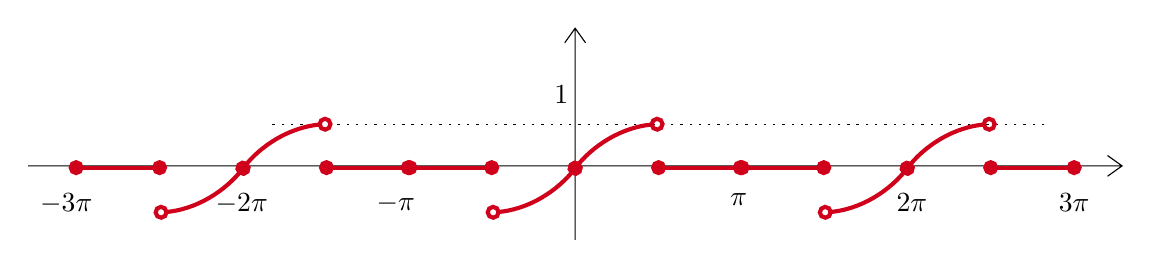
\begin{tikzpicture}[x=0.75pt,y=0.75pt,yscale=-1,xscale=1]
%uncomment if require: \path (0,126); %set diagram left start at 0, and has height of 126

%Straight Lines [id:da10741259255713742] 
\draw  [dash pattern={on 0.84pt off 2.51pt}]  (526.5,59.75) -- (153,59.75) ;
%Shape: Axis 2D [id:dp7770976156065474] 
\draw  (37,79.83) -- (564,79.83)(300.5,13.5) -- (300.5,115.53) (557,74.83) -- (564,79.83) -- (557,84.83) (295.5,20.5) -- (300.5,13.5) -- (305.5,20.5)  ;
%Straight Lines [id:da9173549601591173] 
\draw [color={rgb, 255:red, 208; green, 2; blue, 27 }  ,draw opacity=1 ][line width=1.5]    (380.92,80.67) -- (340.71,80.67) ;
\draw [shift={(340.71,80.67)}, rotate = 180] [color={rgb, 255:red, 208; green, 2; blue, 27 }  ,draw opacity=1 ][fill={rgb, 255:red, 208; green, 2; blue, 27 }  ,fill opacity=1 ][line width=1.5]      (0, 0) circle [x radius= 2.61, y radius= 2.61]   ;
\draw [shift={(380.92,80.67)}, rotate = 180] [color={rgb, 255:red, 208; green, 2; blue, 27 }  ,draw opacity=1 ][fill={rgb, 255:red, 208; green, 2; blue, 27 }  ,fill opacity=1 ][line width=1.5]      (0, 0) circle [x radius= 2.61, y radius= 2.61]   ;
%Curve Lines [id:da4725268586811755] 
\draw [color={rgb, 255:red, 208; green, 2; blue, 27 }  ,draw opacity=1 ][line width=1.5]    (300.5,80.97) .. controls (308.75,70.09) and (323.11,60.82) .. (338.56,59.82) ;
\draw [shift={(340,59.75)}, rotate = 358.21] [color={rgb, 255:red, 208; green, 2; blue, 27 }  ,draw opacity=1 ][line width=1.5]      (0, 0) circle [x radius= 2.61, y radius= 2.61]   ;
\draw [shift={(300.5,80.97)}, rotate = 307.15] [color={rgb, 255:red, 208; green, 2; blue, 27 }  ,draw opacity=1 ][fill={rgb, 255:red, 208; green, 2; blue, 27 }  ,fill opacity=1 ][line width=1.5]      (0, 0) circle [x radius= 2.61, y radius= 2.61]   ;
%Straight Lines [id:da4808528317246443] 
\draw [color={rgb, 255:red, 208; green, 2; blue, 27 }  ,draw opacity=1 ][line width=1.5]    (260.29,80.67) -- (220.08,80.67) ;
\draw [shift={(220.08,80.67)}, rotate = 180] [color={rgb, 255:red, 208; green, 2; blue, 27 }  ,draw opacity=1 ][fill={rgb, 255:red, 208; green, 2; blue, 27 }  ,fill opacity=1 ][line width=1.5]      (0, 0) circle [x radius= 2.61, y radius= 2.61]   ;
\draw [shift={(260.29,80.67)}, rotate = 180] [color={rgb, 255:red, 208; green, 2; blue, 27 }  ,draw opacity=1 ][fill={rgb, 255:red, 208; green, 2; blue, 27 }  ,fill opacity=1 ][line width=1.5]      (0, 0) circle [x radius= 2.61, y radius= 2.61]   ;
%Curve Lines [id:da8687455493649499] 
\draw [color={rgb, 255:red, 208; green, 2; blue, 27 }  ,draw opacity=1 ][line width=1.5]    (300.5,80.97) .. controls (292.26,91.85) and (277.89,101.11) .. (262.44,102.12) ;
\draw [shift={(261,102.18)}, rotate = 178.21] [color={rgb, 255:red, 208; green, 2; blue, 27 }  ,draw opacity=1 ][line width=1.5]      (0, 0) circle [x radius= 2.61, y radius= 2.61]   ;
\draw [shift={(300.5,80.97)}, rotate = 127.15] [color={rgb, 255:red, 208; green, 2; blue, 27 }  ,draw opacity=1 ][fill={rgb, 255:red, 208; green, 2; blue, 27 }  ,fill opacity=1 ][line width=1.5]      (0, 0) circle [x radius= 2.61, y radius= 2.61]   ;

%Straight Lines [id:da599685016533257] 
\draw [color={rgb, 255:red, 208; green, 2; blue, 27 }  ,draw opacity=1 ][line width=1.5]    (540.92,80.67) -- (500.71,80.67) ;
\draw [shift={(500.71,80.67)}, rotate = 180] [color={rgb, 255:red, 208; green, 2; blue, 27 }  ,draw opacity=1 ][fill={rgb, 255:red, 208; green, 2; blue, 27 }  ,fill opacity=1 ][line width=1.5]      (0, 0) circle [x radius= 2.61, y radius= 2.61]   ;
\draw [shift={(540.92,80.67)}, rotate = 180] [color={rgb, 255:red, 208; green, 2; blue, 27 }  ,draw opacity=1 ][fill={rgb, 255:red, 208; green, 2; blue, 27 }  ,fill opacity=1 ][line width=1.5]      (0, 0) circle [x radius= 2.61, y radius= 2.61]   ;
%Curve Lines [id:da4402562566796744] 
\draw [color={rgb, 255:red, 208; green, 2; blue, 27 }  ,draw opacity=1 ][line width=1.5]    (460.5,80.97) .. controls (468.75,70.09) and (483.11,60.82) .. (498.56,59.82) ;
\draw [shift={(500,59.75)}, rotate = 358.21] [color={rgb, 255:red, 208; green, 2; blue, 27 }  ,draw opacity=1 ][line width=1.5]      (0, 0) circle [x radius= 2.61, y radius= 2.61]   ;
\draw [shift={(460.5,80.97)}, rotate = 307.15] [color={rgb, 255:red, 208; green, 2; blue, 27 }  ,draw opacity=1 ][fill={rgb, 255:red, 208; green, 2; blue, 27 }  ,fill opacity=1 ][line width=1.5]      (0, 0) circle [x radius= 2.61, y radius= 2.61]   ;
%Straight Lines [id:da08510756351773896] 
\draw [color={rgb, 255:red, 208; green, 2; blue, 27 }  ,draw opacity=1 ][line width=1.5]    (420.29,80.67) -- (380.08,80.67) ;
\draw [shift={(380.08,80.67)}, rotate = 180] [color={rgb, 255:red, 208; green, 2; blue, 27 }  ,draw opacity=1 ][fill={rgb, 255:red, 208; green, 2; blue, 27 }  ,fill opacity=1 ][line width=1.5]      (0, 0) circle [x radius= 2.61, y radius= 2.61]   ;
\draw [shift={(420.29,80.67)}, rotate = 180] [color={rgb, 255:red, 208; green, 2; blue, 27 }  ,draw opacity=1 ][fill={rgb, 255:red, 208; green, 2; blue, 27 }  ,fill opacity=1 ][line width=1.5]      (0, 0) circle [x radius= 2.61, y radius= 2.61]   ;
%Curve Lines [id:da9678260771297018] 
\draw [color={rgb, 255:red, 208; green, 2; blue, 27 }  ,draw opacity=1 ][line width=1.5]    (460.5,80.97) .. controls (452.26,91.85) and (437.89,101.11) .. (422.44,102.12) ;
\draw [shift={(421,102.18)}, rotate = 178.21] [color={rgb, 255:red, 208; green, 2; blue, 27 }  ,draw opacity=1 ][line width=1.5]      (0, 0) circle [x radius= 2.61, y radius= 2.61]   ;
\draw [shift={(460.5,80.97)}, rotate = 127.15] [color={rgb, 255:red, 208; green, 2; blue, 27 }  ,draw opacity=1 ][fill={rgb, 255:red, 208; green, 2; blue, 27 }  ,fill opacity=1 ][line width=1.5]      (0, 0) circle [x radius= 2.61, y radius= 2.61]   ;

%Straight Lines [id:da6685458363363093] 
\draw [color={rgb, 255:red, 208; green, 2; blue, 27 }  ,draw opacity=1 ][line width=1.5]    (220.92,80.67) -- (180.71,80.67) ;
\draw [shift={(180.71,80.67)}, rotate = 180] [color={rgb, 255:red, 208; green, 2; blue, 27 }  ,draw opacity=1 ][fill={rgb, 255:red, 208; green, 2; blue, 27 }  ,fill opacity=1 ][line width=1.5]      (0, 0) circle [x radius= 2.61, y radius= 2.61]   ;
\draw [shift={(220.92,80.67)}, rotate = 180] [color={rgb, 255:red, 208; green, 2; blue, 27 }  ,draw opacity=1 ][fill={rgb, 255:red, 208; green, 2; blue, 27 }  ,fill opacity=1 ][line width=1.5]      (0, 0) circle [x radius= 2.61, y radius= 2.61]   ;
%Curve Lines [id:da31702343634185315] 
\draw [color={rgb, 255:red, 208; green, 2; blue, 27 }  ,draw opacity=1 ][line width=1.5]    (140.5,80.97) .. controls (148.75,70.09) and (163.11,60.82) .. (178.56,59.82) ;
\draw [shift={(180,59.75)}, rotate = 358.21] [color={rgb, 255:red, 208; green, 2; blue, 27 }  ,draw opacity=1 ][line width=1.5]      (0, 0) circle [x radius= 2.61, y radius= 2.61]   ;
\draw [shift={(140.5,80.97)}, rotate = 307.15] [color={rgb, 255:red, 208; green, 2; blue, 27 }  ,draw opacity=1 ][fill={rgb, 255:red, 208; green, 2; blue, 27 }  ,fill opacity=1 ][line width=1.5]      (0, 0) circle [x radius= 2.61, y radius= 2.61]   ;
%Straight Lines [id:da9353356461505657] 
\draw [color={rgb, 255:red, 208; green, 2; blue, 27 }  ,draw opacity=1 ][line width=1.5]    (100.29,80.67) -- (60.08,80.67) ;
\draw [shift={(60.08,80.67)}, rotate = 180] [color={rgb, 255:red, 208; green, 2; blue, 27 }  ,draw opacity=1 ][fill={rgb, 255:red, 208; green, 2; blue, 27 }  ,fill opacity=1 ][line width=1.5]      (0, 0) circle [x radius= 2.61, y radius= 2.61]   ;
\draw [shift={(100.29,80.67)}, rotate = 180] [color={rgb, 255:red, 208; green, 2; blue, 27 }  ,draw opacity=1 ][fill={rgb, 255:red, 208; green, 2; blue, 27 }  ,fill opacity=1 ][line width=1.5]      (0, 0) circle [x radius= 2.61, y radius= 2.61]   ;
%Curve Lines [id:da990279944542586] 
\draw [color={rgb, 255:red, 208; green, 2; blue, 27 }  ,draw opacity=1 ][line width=1.5]    (140.5,80.97) .. controls (132.26,91.85) and (117.89,101.11) .. (102.44,102.12) ;
\draw [shift={(101,102.18)}, rotate = 178.21] [color={rgb, 255:red, 208; green, 2; blue, 27 }  ,draw opacity=1 ][line width=1.5]      (0, 0) circle [x radius= 2.61, y radius= 2.61]   ;
\draw [shift={(140.5,80.97)}, rotate = 127.15] [color={rgb, 255:red, 208; green, 2; blue, 27 }  ,draw opacity=1 ][fill={rgb, 255:red, 208; green, 2; blue, 27 }  ,fill opacity=1 ][line width=1.5]      (0, 0) circle [x radius= 2.61, y radius= 2.61]   ;


% Text Node
\draw (41.5,92.13) node [anchor=north west][inner sep=0.75pt]  [font=\normalsize]  {$-3\pi $};
% Text Node
\draw (126.07,92.13) node [anchor=north west][inner sep=0.75pt]  [font=\normalsize]  {$-2\pi $};
% Text Node
\draw (203.6,92.13) node [anchor=north west][inner sep=0.75pt]  [font=\normalsize]  {$-\pi $};
% Text Node
\draw (374.04,92.13) node [anchor=north west][inner sep=0.75pt]  [font=\normalsize]  {$\pi $};
% Text Node
\draw (454.1,92.13) node [anchor=north west][inner sep=0.75pt]  [font=\normalsize]  {$2\pi $};
% Text Node
\draw (532.3,92.13) node [anchor=north west][inner sep=0.75pt]  [font=\normalsize]  {$3\pi $};
% Text Node
\draw (289.25,39.76) node [anchor=north west][inner sep=0.75pt]  [font=\normalsize]  {$1$};


\end{tikzpicture}
\end{figure}
\FloatBarrier

\item Poiché

\begin{equation*}
\int ^{\pi }_{-\pi } f^{2}( x) dx< +\infty \ \ \Rightarrow \ \ f\in L^{2}([ -\pi ,\pi ])
\end{equation*}

allora la serie di Fourier converge in media quadratica.
\item $f$ è una funzione regolare a tratti in $[ -\pi ,\pi ]$, allora converge puntualmente $\forall x\in \mathbb{R}$.

Più precisamente converge puntualmente a $f( x) ,\ \forall x\neq ( 2k+1)\frac{\pi }{2} ,\ k\in \mathbb{Z}$, mentre converge a $\frac{1}{2} ,\ \forall x=( 2k+1)\frac{\pi }{2} ,\ k\in \mathbb{Z}$.
\item Non c'è convergenza uniforme perché $f$ non è continua su $\mathbb{R}$.
\item $f$ è dispari, allora $a_{n} =0,\ \forall n\in \mathbb{N}$.

\begin{equation*}
\begin{aligned}
b_{n} & =\frac{2}{\pi }\int ^{\pi }_{0} f( x)\sin( nx) dx\\
 & =\frac{2}{\pi }\int ^{\frac{\pi }{2}}_{0} f( x)\sin( nx) dx=\frac{2}{\pi }\int ^{\frac{\pi }{2}}_{0}\sin x\sin( nx) dx
\end{aligned}
\end{equation*}

Possiamo fare un integrale ciclico o usare le formule di Werner. Usiamo il primo\begin{align*}
\frac{2}{\pi }\int ^{\frac{\pi }{2}}_{0}\sin x\sin( nx) dx & \overset{\text{ipp}}{=}\frac{2}{\pi }\left\{\cancel{[ -\cos x\sin( nx)]^{\frac{\pi }{2}}_{0}} +n\int ^{\frac{\pi }{2}}_{0}\cos x\cos( nx) dx\right\}\\
 & =\frac{2n}{\pi }\int ^{\frac{\pi }{2}}_{0}\cos x\cos( nx) dx\\
 & \overset{\text{ipp}}{=}\frac{2n}{\pi }\left\{[\sin x\cos( nx)]^{\frac{\pi }{2}}_{0} +n\int ^{\frac{\pi }{2}}_{0}\sin x\sin( nx) dx\right\}\\
 & =\frac{2n}{\pi }\cos\left( n\frac{\pi }{2}\right) +\frac{2n^{2}}{\pi }\int ^{\frac{\pi }{2}}_{0}\sin x\sin( nx) dx\\
 & \\
\Rightarrow \ \ b_{n} & =\frac{2n}{\pi }\cos\left( n\frac{\pi }{2}\right) +n^{2} b_{n}\\
\left( 1-n^{2}\right) b_{n} & =\frac{2n}{\pi }\cos\left( n\frac{\pi }{2}\right)
\end{align*}

per $n\neq 1$\begin{equation*}
b_{n} =\frac{2}{\pi }\frac{n}{1-n^{2}}\cos\left( n\frac{\pi }{2}\right) =\begin{cases}
( -1)^{\frac{n}{2}}\frac{2}{\pi }\frac{n}{1-n^{2}} , & n\ \text{pari}\\
0, & n\ \text{dispari}
\end{cases}
\end{equation*}

per $n=1$\begin{equation*}
\begin{aligned}
b_{1} & =\frac{2}{\pi }\int ^{\pi }_{0} f( x)\sin( x) dx=\frac{2}{\pi }\int ^{\frac{\pi }{2}}_{0}\sin^{2}( x) dx=\frac{2}{\pi }\int ^{\frac{\pi }{2}}_{0}\frac{1-\cos 2x}{2} dx\\
 & =\frac{1}{\pi }\left[ x-\frac{1}{2}\sin( 2x)\right]^{\frac{\pi }{2}}_{0} =\frac{1}{\pi }\left[\frac{\pi }{2} -0+0-0\right] =\frac{1}{2}
\end{aligned}
\end{equation*}

Allora $( n=2k,\ k\in \mathbb{N})$:

\begin{equation*}
F( x) =\frac{1}{2}\sin x+\frac{2}{\pi }\sum ^{+\infty }_{k=1}( -1)^{k}\frac{2k}{1-4k^{2}}\sin( 2kx)
\end{equation*}
\item In $x=\frac{\pi }{4}$ la $f$ è continua, quindi la $F( x)$ converge puntualmente a $f( x)$.\begin{align*}
F\left(\frac{\pi }{4}\right) & =\sin\left(\frac{\pi }{4}\right) =\frac{1}{\sqrt{2}}\\
F\left(\frac{\pi }{4}\right) & =\frac{1}{2}\sin\left(\frac{\pi }{4}\right) +\frac{4}{\pi }\sum ^{+\infty }_{k=1}( -1)^{k-1}\frac{k}{4k^{2} -1}\sin\left( k\frac{\pi }{2}\right)\\
\Rightarrow \ \ \frac{1}{\sqrt{2}} & =\frac{1}{2\sqrt{2}} +\frac{4}{\pi }\sum ^{+\infty }_{k=0}( -1)^{k-1}\frac{k}{4k^{2} -1}\sin\left( k\frac{\pi }{2}\right)
\end{align*}

Notiamo che la serie si annulla ogni volta che $k$ è pari, essendo il seno di $\pi ,2\pi ,3\pi \dotsc $, quindi possiamo sommare direttamente sui dispari

\begin{equation*}
\begin{aligned}
\frac{1}{\sqrt{2}} & =\frac{1}{2\sqrt{2}} +\frac{4}{\pi }\sum ^{+\infty }_{k=0}\cancel{( -1)^{( 2k+1) -1}}\frac{2k+1}{4( 2k+1)^{2} -1}\underbrace{\sin\left(( 2k+1)\frac{\pi }{2}\right)}_{( -1)^{k}}\\
\frac{1}{2\sqrt{2}} & =\frac{4}{\pi }\sum ^{+\infty }_{k=0}\frac{2k+1}{4( 2k+1)^{2} -1}( -1)^{k}\\
 & \Rightarrow \ \ \sum ^{+\infty }_{k=0}\frac{2k+1}{4( 2k+1)^{2} -1}( -1)^{k} =\frac{\pi }{8\sqrt{2}}
\end{aligned}
\end{equation*}
\item $f\in L^{2}([ -\pi ,\pi ])$ allora vale l'identità di Parseval

\begin{equation*}
\frac{1}{\pi }\int ^{\pi }_{-\pi }| f( x)| ^{2} dx=\frac{a^{2}_{0}}{2} +\sum\limits ^{\infty }_{n=1}\left( a^{2}_{n} +b^{2}_{n}\right)
\end{equation*}

Nel nostro caso $f$ è dispari, $a_{n} =0,\ \forall n\in \mathbb{N}$, e si ha

\begin{equation*}
\underbrace{\frac{1}{\pi }\int ^{\pi }_{-\pi }| f( x)| ^{2} dx}_{A} =\underbrace{\sum\limits ^{\infty }_{n=1} b^{2}_{n}}_{B}
\end{equation*}

Termine $A$\begin{equation*}
\begin{aligned}
\frac{1}{\pi }\int ^{\pi }_{-\pi }| f( x)| ^{2} dx & =\frac{1}{\pi }\int ^{\frac{\pi }{2}}_{-\frac{\pi }{2}}\sin^{2}( x) dx=\frac{1}{\pi }\int ^{\frac{\pi }{2}}_{-\frac{\pi }{2}}\frac{1-\cos( 2x)}{2} dx\\
 & =\frac{1}{2\pi }\left[ x-\frac{1}{2}\sin( 2x)\right]^{\pi /2}_{-\pi /2} =\frac{1}{2\pi }\left[\frac{\pi }{2} +\frac{\pi }{2}\right] =\frac{1}{2}
\end{aligned}
\end{equation*}

Termine $B$\begin{equation*}
\begin{aligned}
\sum\limits ^{\infty }_{n=1} b^{2}_{n} & =b^{2}_{1} +\sum\limits ^{\infty }_{n=1} b^{2}_{2n}\\
 & =\left(\frac{1}{2}\right)^{2} +\frac{4}{\pi ^{2}}\sum\limits ^{\infty }_{n=1}\frac{4n^{2}}{\left( 4n^{2} -1\right)^{2}}
\end{aligned}
\end{equation*}

Ugualiamo i termini

\begin{equation*}
\frac{1}{2} =\frac{1}{4} +\frac{4}{\pi ^{2}}\sum\limits ^{\infty }_{n=1}\frac{4n^{2}}{\left( 4n^{2} -1\right)^{2}} \ \ \Rightarrow \ \ \sum\limits ^{\infty }_{n=1}\frac{4n^{2}}{\left( 4n^{2} -1\right)^{2}} =\frac{\pi ^{2}}{64}
\end{equation*}
\end{enumerate}
\Soluzione

Notiamo che sono serie convergenti, perché asintotiche a $\frac{1}{n^{\alpha }}$ con $\alpha  >1$.

$f$ è pari, allora $b_{n} =0,\ \forall n\geqslant 1$.
\begin{align*}
a_{0} & =\frac{2}{\pi }\int ^{\pi }_{0} xdx=\frac{2}{\pi }\frac{\pi ^{2}}{2} =\pi \\
 & \\
a_{n} & \overset{n\geqslant 1}{=}\frac{1}{\pi }\int ^{\pi }_{-\pi } f( x)\cos( nx) dx=\frac{2}{\pi }\int ^{\pi }_{0} x\cos( nx) dx\\
 & \overset{\text{ipp}}{=}\frac{2}{\pi }\left\{\cancel{\left[\frac{x\sin( nx)}{n}\right]^{\pi }_{0}} -\frac{1}{n}\int ^{\pi }_{0}\sin( nx) dx\right\}\\
 & =-\frac{2}{\pi n}\left[ -\frac{\cos( nx)}{n}\right]^{\pi }_{0} =\frac{2}{\pi n^{2}}\left[( -1)^{n} -1\right] =\begin{cases}
0, & n\ \text{pari}\\
-\frac{4}{\pi n^{2}} , & n\ \text{dispari}
\end{cases}
\end{align*}
Allora
\begin{equation*}
F( x) =\frac{\pi }{2} -\frac{4}{\pi }\sum\limits ^{\infty }_{n=0}\frac{\cos[( 2n+1) x]}{( 2n+1)^{2}}
\end{equation*}
$f\in L^{2}( Q) \Rightarrow $ vale l'identità di Parseval
\begin{equation*}
\underbrace{\frac{1}{\pi }\int ^{\pi }_{-\pi }| f( x)| ^{2} dx}_{A} =\underbrace{\frac{a^{2}_{0}}{2} +\sum\limits ^{\infty }_{n=1}\left( a^{2}_{n} +b^{2}_{n}\right)}_{B}
\end{equation*}
Termine $A$
\begin{equation*}
A=\frac{1}{\pi }\int ^{\pi }_{-\pi } x^{2} dx=\frac{1}{\pi }\left[\frac{x^{3}}{3}\right]^{\pi }_{-\pi } =\frac{1}{\pi }\left\{\frac{\pi ^{3}}{3} +\frac{\pi ^{3}}{3}\right\} =\frac{2\pi ^{2}}{3}
\end{equation*}
Termine $B$
\begin{equation*}
B=\frac{a^{2}_{0}}{2} +\sum\limits ^{\infty }_{n=1}\left( a^{2}_{n} +\cancel{b^{2}_{n}}\right) =\frac{\pi ^{2}}{2} +\frac{16}{\pi ^{2}}\sum\limits ^{\infty }_{\textcolor[rgb]{0.82,0.01,0.11}{n=0}}\frac{1}{( 2n+1)^{4}}
\end{equation*}
Uguagliamo
\begin{equation*}
\frac{2\pi ^{2}}{3} -\frac{\pi ^{2}}{2} =\frac{16}{\pi ^{2}}\sum\limits ^{\infty }_{n=0}\frac{1}{( 2n+1)^{4}} \ \ \Rightarrow \ \ \sum\limits ^{\infty }_{n=0}\frac{1}{( 2n+1)^{4}} =\frac{\pi ^{4}}{96}
\end{equation*}
Osserviamo che
\begin{equation*}
\underbrace{\sum\limits ^{\infty }_{n=0}\frac{1}{( 2n+1)^{4}}}_{\text{sui dispari}} =\underbrace{\sum\limits ^{\infty }_{n=1}\frac{1}{n^{4}}}_{\text{su tutti}} -\underbrace{\sum\limits ^{\infty }_{n=1}\frac{1}{( 2n)^{4}}}_{\text{sui pari}} =\sum\limits ^{\infty }_{n=1}\frac{1}{n^{4}} -\frac{1}{2^{4}}\sum\limits ^{\infty }_{n=1}\frac{1}{n^{4}} =\left( 1-\frac{1}{2^{4}}\right)\sum\limits ^{\infty }_{n=1}\frac{1}{n^{4}}
\end{equation*}
allora
\begin{equation*}
\sum\limits ^{\infty }_{n=1}\frac{1}{n^{4}} =\frac{\sum\limits ^{\infty }_{n=0}\frac{1}{( 2n+1)^{4}}}{1-\frac{1}{2^{4}}} =\frac{\frac{\pi ^{4}}{96}}{1-\frac{1}{2^{4}}} =\frac{\pi ^{4}}{90}
\end{equation*}
\Soluzione

La funzione è dispari, per cui $a_{n} =0,\forall n$.
\begin{align*}
b_{n} & =\frac{1}{\pi }\int ^{\pi }_{-\pi } f( x)\sin( nx) dx\\
 & =\frac{2}{\pi }\int ^{\pi }_{0} f( x)\sin( nx) dx\\
 & =\frac{2}{\pi }\int ^{\pi }_{0}\left( -x^{2} +x\pi \right)\sin( nx) dx\\
 & =\frac{2}{\pi }\left\{\cancel{\left[\left( -x^{2} +x\pi \right) \cdotp \left( -\frac{\cos( nx)}{n}\right)\right]^{\pi }_{0}} +\frac{1}{n}\int ^{\pi }_{0}\cos( nx)( \pi -2x) dx\right\}\\
 & =\frac{2}{\pi n}\left\{\cancel{\left[( \pi -2x) \cdotp \frac{\sin( nx)}{n}\right]^{\pi }_{0}} +2\int ^{\pi }_{0}\frac{\sin( nx)}{n} dx\right\}\\
 & =\frac{4}{\pi n^{2}}\left\{\int ^{\pi }_{0}\sin( nx) dx\right\}\\
 & =\frac{4}{\pi n^{2}}\left[ -\frac{\cos( nx)}{n}\right]^{\pi }_{0}\\
 & =\frac{4}{\pi n^{3}}[ 1-\cos( n\pi )]\\
 & =\frac{4}{\pi n^{3}}\left[ 1-( -1)^{n}\right] =\begin{cases}
\frac{8}{\pi n^{3}} , & n\ \text{dispari}\\
0, & n\ \text{pari}
\end{cases}
\end{align*}
La serie di Fourier cercata è
\begin{align*}
F( x) & =\sum\limits ^{\infty }_{n=1} b_{n}\sin( nx)\\
 & =\sum\limits ^{\infty }_{n=1}\frac{4}{\pi n^{3}}\left[ 1-( -1)^{n}\right]\sin( nx)\\
 & =\sum\limits ^{\infty }_{n=0}\frac{8}{\pi ( 2n+1)^{3}}\sin(( 2n+1) x)
\end{align*}
Scriviamo l'identità di Parseval
\begin{align*}
\frac{1}{\pi }\int ^{\pi }_{-\pi }[ f( x)]^{2} dx & =\cancel{\frac{a^{2}_{0}}{2}} +\sum\limits ^{\infty }_{n=1}\left(\cancel{a^{2}_{n}} +b^{2}_{n}\right)\\
\frac{1}{\pi } \cdotp 2\int ^{\pi }_{0}\left( x\pi -x^{2}\right)^{2} dx & =\sum\limits ^{\infty }_{n=1} b^{2}_{n}\\
\frac{2}{\pi }\int ^{\pi }_{0}\left[ x^{4} +x^{2} \pi ^{2} -2\pi x^{3}\right) dx & =\sum\limits ^{\infty }_{n=0}\frac{8^{2}}{\pi ^{2}( 2n+1)^{6}}\\
\frac{2}{\pi }\left[\frac{\pi ^{5}}{5} +\frac{\pi ^{3}}{3} \pi ^{2} -2\pi \frac{\pi ^{4}}{4}\right] & =\sum\limits ^{\infty }_{n=0}\frac{64}{\pi ^{2}( 2n+1)^{6}}\\
\frac{\pi ^{4}}{15} & =\frac{64}{\pi ^{2}}\sum\limits ^{\infty }_{n=0}\frac{1}{( 2n+1)^{6}}\\
 & \Rightarrow \ \ \sum\limits ^{\infty }_{n=0}\frac{1}{( 2n+1)^{6}} =\frac{\pi ^{6}}{960}
\end{align*}
Per il secondo risultato sappiamo che la somma su tutti i naturali è come sommare tutti i dispari e tutti i pari. Chiamiamo $J$ la serie cercata
\begin{align*}
\sum\limits ^{\infty }_{n=1}\frac{1}{n^{6}} & =\sum\limits ^{\infty }_{n=0}\frac{1}{( 2n+1)^{6}} +\sum\limits ^{\infty }_{n=1}\frac{1}{( 2n)^{6}}\\
J & =\frac{\pi ^{6}}{960} +\frac{1}{2^{6}} J\\
 & \Rightarrow \ \ J=\frac{\frac{\pi ^{6}}{960}}{1-\frac{1}{2^{6}}} =\frac{\pi ^{6}}{945}
\end{align*}
\Soluzione

Disegnamo il grafico di
\begin{equation*}
f_{n}( x) =\begin{cases}
ne^{n( x-1)} , & x\leqslant 1\\
0, & x >1
\end{cases}
\end{equation*}
\fg{0.7}{12-4}
\begin{enumerate}
\item Fissiamo $x_{0} \in \mathbb{R}$
\begin{enumerate}
\item Se $x_{0} =1\Rightarrow f_{n}( 1) =n\xrightarrow{n\rightarrow +\infty } +\infty $.
\item Se $x_{0} \neq 1\Rightarrow f_{n}( x_{0})\xrightarrow{n\rightarrow +\infty } 0$.
\end{enumerate}

Quindi converge puntualmente alla funzione limite $f( x) \equiv 0\ \forall x\neq 1$.
\item $\forall \varphi \in D(\mathbb{R})$, cioè per ogni $\varphi $ a supporto compatto in $\mathbb{R}$,\begin{align*}
\langle f_{n} ,\varphi \rangle  & =\int _{\mathbb{R}} f_{n}( x) \varphi ( x) dx\\
 & =\int ^{1}_{-\infty } ne^{n( x-1)} \varphi ( x) dx\\
 & \overset{\text{ipp}}{=}\left[ e^{n( x-1)} \varphi ( x)\right]^{1}_{-\infty } -\int ^{1}_{-\infty } e^{n( x-1)} \varphi '( x) dx\\
 & =\varphi ( 1) -\int ^{1}_{-\infty } e^{n( x-1)} \varphi '( x) dx
\end{align*}

Obiettivo: calcolare il limite per $n\rightarrow +\infty $\begin{align*}
\lim\limits _{n\rightarrow +\infty } \langle f_{n} ,\varphi \rangle  & =\lim\limits _{n\rightarrow +\infty }\left[ \varphi ( 1) -\int ^{1}_{-\infty } e^{n( x-1)} \varphi '( x) dx\right]\\
 & =\varphi ( 1) -\lim\limits _{n\rightarrow +\infty }\int ^{1}_{-\infty } e^{n( x-1)} \varphi '( x) dx\\
 & \overset{\text{Dom}}{=} \varphi ( 1) -\int ^{1}_{-\infty }\underbrace{\lim\limits _{n\rightarrow +\infty } e^{n( x-1)} \varphi '( x)}_{=0} dx=\varphi ( 1)
\end{align*}

Posso applicare il teorema della convergenza dominata perché $\varphi \in D(\mathbb{R})$. $\exists M$ tale che $| \varphi '( x)| < M,\ \forall x\in \mathbb{R}$.

\begin{equation*}
\left| e^{n( x-1)} \varphi '( x)\right| \leqslant Me^{x-1} \in L^{1}(( -\infty ,1))
\end{equation*}

Quindi concludiamo che

\begin{equation*}
f_{n}\xrightarrow[n\rightarrow +\infty ]{D'(\mathbb{R})} \delta _{1} \ 
\end{equation*}

nel senso delle distribuzioni.
\end{enumerate}
\Soluzione
\begin{enumerate}
\item Studiamo il limite puntuale di

\begin{gather*}
f_{n,\alpha }( x) =n^{\alpha }\sqrt{1-n| x| } \cdotp \chi _{\left[ -\frac{1}{n} ,\frac{1}{n}\right]}( x)\\
\lim\limits _{n\rightarrow +\infty } f_{n,\alpha }( x) =\begin{cases}
+\infty , & x=0\\
0, & x\neq 0
\end{cases} \ \ \Rightarrow \ \ f_{n,\alpha }( x)\xrightarrow{n\rightarrow +\infty } f( x) \equiv 0\ \text{q.o.}
\end{gather*}
\item Calcoliamo il limite della norma elevata alla $p$ della differenza e per quali condizioni tende a zero\begin{align*}
 & \int _{\mathbb{R}}[ f_{n,\alpha }( x) -0]^{p} d\xrightarrow{n\rightarrow +\infty } 0\\
 & \Leftrightarrow \ \ 2\int ^{1/n}_{0} n^{\alpha p}( 1-nx)^{p/2} dx\xrightarrow{n\rightarrow +\infty } 0\\
 & \Leftrightarrow \ \ 2n^{\alpha p}\int ^{1/n}_{0}( 1-nx)^{p/2} dx\xrightarrow{n\rightarrow +\infty } 0\\
 & \Leftrightarrow \ \ 2n^{\alpha p}\left[\frac{( 1-nx)^{p/2+1}}{\frac{p}{2} +1} \cdotp \left(\frac{1}{-n}\right)\right]^{1/n}_{0}\xrightarrow{n\rightarrow +\infty } 0\\
 & \Leftrightarrow \ \ 2n^{\alpha p} \cdotp \frac{1}{n\left(\frac{p}{2} +1\right)}\xrightarrow{n\rightarrow +\infty } 0\\
 & \Leftrightarrow \ \ C\cdotp n^{\alpha p-1}\xrightarrow{n\rightarrow +\infty } 0\\
 & \Leftrightarrow \ \ \alpha p-1< 0\\
 & \Leftrightarrow \ \ \alpha < \frac{1}{p} \land \alpha  >0
\end{align*}

Notiamo infine che le $f_{n,\alpha }$ non sono limitate, quindi\begin{equation*}
f_{n,\alpha }\cancel{\xrightarrow[n\rightarrow +\infty ]{L^{\infty }(\mathbb{R})}} 0
\end{equation*}
\item Per $\alpha =1$

\begin{equation*}
f_{n,1}( x) =n\sqrt{1-n| x| } \cdotp \chi _{\left[ -\frac{1}{n} ,\frac{1}{n}\right]}( x)
\end{equation*}

Per ogni $\varphi \in D(\mathbb{R})$\begin{align*}
\langle f_{n,1} ,\varphi \rangle  & =\int _{\mathbb{R}} f_{n,1}( x) \varphi ( x) dx=n\int ^{\frac{1}{n}}_{-\frac{1}{n}}\sqrt{1-n| x| } \cdotp \varphi ( x) dx\\
 & =n\left\{\int ^{0}_{-\frac{1}{n}}\sqrt{1+nx} \cdotp \varphi ( x) dx+\int ^{\frac{1}{n}}_{0}\sqrt{1-nx} \cdotp \varphi ( x) dx\right\}\\
 & \begin{array}{ c c }
\varphi ( x) & \varphi '( x)\\
\frac{1}{n}\frac{( 1+nx)^{3/2}}{\frac{3}{2}} & \sqrt{1+nx}\\
-\frac{1}{n}\frac{( 1-nx)^{3/2}}{\frac{3}{2}} & \sqrt{1-nx}
\end{array}\\
 & \overset{\text{ipp}}{=} n\left\{\left[\frac{2}{3n}\sqrt{(1+nx)^{3}} \varphi (x)\right]^{0}_{-1/n} -\frac{2}{3n}\int ^{0}_{-\frac{1}{n}}\sqrt{(1+nx)^{3}} \varphi '(x)dx+\right. \\
 & \left. +\left[ -\frac{2}{3n}\sqrt{(1-nx)^{3}} \varphi (x)\right]^{1/n}_{0} +\frac{2}{3n}\int ^{1/n}_{0}\sqrt{(1+nx)^{3}} \varphi '(x)dx\right\}\\
 & =2\cdotp \frac{2}{3} \varphi ( 0) +\frac{2}{3}\left\{-\int ^{0}_{-\frac{1}{n}}\sqrt{(1+nx)^{3}} \varphi '(x)dx+\int ^{1/n}_{0}\sqrt{(1+nx)^{3}} \varphi '(x)dx\right\}
\end{align*}

Quindi

\begin{equation*}
\lim\limits _{n\rightarrow +\infty } \langle f_{n,1} ,\varphi \rangle =\frac{4}{3} \varphi ( 0) +\frac{2}{3}\lim\limits _{n\rightarrow +\infty }\left\{-\int ^{0}_{-\frac{1}{n}} \dotsc dx+\int ^{1/n}_{0} \dotsc dx\right\}
\end{equation*}

A questo punto osserviamo che

\begin{equation*}
\varphi \in D(\mathbb{R}) \ \ \Rightarrow \ \ M=\max_{x\in [ -1,1]} \varphi ( x)
\end{equation*}

Con un ragionamento analogo a prima\begin{equation*}
\Rightarrow \ \ f_{n,1}\xrightarrow[n\rightarrow +\infty ]{D'(\mathbb{R})}\frac{4}{3} \delta _{0}
\end{equation*}
\end{enumerate}
\chapter{Esercitazione 7 - Boella}
\ParteEsercizi
\Esercizio{}

Calcolare la derivata nel senso delle distribuzioni di
\begin{equation*}
f(x)=\arctan\left(\frac{1}{x}\right)
\end{equation*}
\Esercizio{}

Calcolare la derivata prima e seconda nel senso delle distribuzioni in $D'( 0,5)$ di
\begin{equation*}
f(x)=\begin{cases}
x+x^{2} , & 0< x< 2\\
6, & 2< x< 5
\end{cases}
\end{equation*}
\Esercizio{}

Trovare l'equivalente in $D'(\mathbb{R} )$ di
\begin{equation*}
u(x)=x\delta '_{0} (x)
\end{equation*}
\Esercizio{}

Calcolare il limite delle $f_{n}$ in $L^{p} (\mathbb{R} )$, $D'(\mathbb{R} )$ e $\mathcal{S} '(\mathbb{R} )$ di\footnote{Dove $H$ indica la funzione di Heaviside.}
\begin{equation*}
g(x)=H(x)e^{-x} \ \ \ \ f_{n} (x)=g(x)*\chi _{(0,n)}
\end{equation*}
\Esercizio{}

Calcolare la serie di Fourier associata alla funzione $2\pi $-periodica dispari
\begin{equation*}
f(x)=\begin{cases}
1, & 0< x< \pi \\
-1, & -\pi < x< 0
\end{cases}
\end{equation*}
\ParteSoluzioni
\Soluzione

Dato che $f\in L^{1}_{\mathrm{loc}} (\mathbb{R} )\Rightarrow f\in D'(\mathbb{R} )$.

Sappiamo anche che $f\in \mathcal{S} '(\mathbb{R})$, lo spazio delle distribuzioni temperate.

\fg{0.7}{13-1}

Calcolo quindi la derivata nel senso delle distribuzioni. Ricordiamo innanzitutto che
\begin{equation*}
\frac{d}{dx}\arctan\left(\frac{1}{x}\right) =-\frac{1}{1+\left(\frac{1}{x}\right)^{2}}\frac{1}{x^{2}} =-\frac{1}{1+x^{2}}
\end{equation*}
Calcoliamo
\begin{align*}
\langle f',\varphi \rangle  & =-\langle f,\varphi '\rangle =-\int _{\mathbb{R}}\arctan\left(\frac{1}{x}\right) \varphi '(x)dx=\\
 & =-\int ^{0}_{-\infty }\arctan\left(\frac{1}{x}\right) \varphi '(x)dx-\int ^{+\infty }_{0}\arctan\left(\frac{1}{x}\right) \varphi '(x)dx=\\
 & \overset{\text{ipp}}{=} -\left[\arctan\left(\frac{1}{x}\right) \varphi (x)\right]^{0}_{-\infty } +\int ^{+\infty }_{0}\frac{-1}{1+x^{2}} \varphi ( x) dx\\
 & \ \ \ \ \ -\left[\arctan\left(\frac{1}{x}\right) \varphi (x)\right]^{+\infty }_{0} +\int ^{+\infty }_{0}\frac{-1}{1+x^{2}} \varphi ( x) dx\\
 & =\frac{\pi }{2} \varphi ( 0) +\frac{\pi }{2} \varphi ( 0) +\int _{\mathbb{R}}\frac{-1}{1+x^{2}} \varphi (x)dx\\
 & =\pi \langle \delta _{0} ,\varphi \rangle +\langle \frac{-1}{1+x^{2}} ,\varphi \rangle =\langle \pi \delta _{0} -\frac{1}{1+x^{2}} ,\varphi \rangle 
\end{align*}
Quindi
\begin{equation*}
f'(x)\overset{D'}{=} \pi \delta _{0} -\frac{1}{1+x^{2}}
\end{equation*}
che può essere rappresentata come la funzione $1/\left( 1+x^{2}\right)$ con un salto in $x=0$ verso l'alto di ampiezza $\pi $.
\Soluzione

Dato che $f\in L^{1}_{\mathrm{loc}} (0,5)\Rightarrow f\in D'(0,5)$.

\fg{0.7}{13-2}

Questo significa che la funzione $\varphi (x)$ sarà identicamente nulla su qualsiasi intervallo esterno a $(0,5)$, cioé in particolare $\varphi ( 0) =\varphi ( 5) =0$.
\begin{align*}
\langle f',\varphi \rangle  & =-\langle f,\varphi '\rangle =-\int ^{5}_{0} f(x)\varphi '(x)dx\\
 & =-\left\{\int ^{2}_{0} (x+x^{2} )\varphi '(x)dx+\int ^{5}_{2} 6\varphi '(x)dx\right\}\\
 & \overset{\text{ipp}}{=} -\left\{\left[ (x+x^{2} )\varphi (x)\right]^{2}_{0} -\int ^{2}_{0} (1+2x)\varphi (x)dx+[ 6\varphi (x)]^{5}_{2}\right\}\\
 & =-\left\{\cancel{6\varphi ( 2)} -0-\int ^{2}_{0}( 1+2x) \varphi ( x) dx+\cancel{6\varphi ( 5)} -\cancel{6\varphi ( 2)}\right\}\\
 & =\int ^{2}_{0}( 1+2x) \varphi ( x) dx
\end{align*}
Definiamo
\begin{equation*}
g(x)=\begin{cases}
2x+1, & 0< x< 2\\
0, & 2< x< 5
\end{cases} \ \ \Rightarrow \ \ \langle f',\varphi \rangle =\int _{\mathbb{R}} g( x) \varphi ( x) dx=\langle g,\varphi \rangle 
\end{equation*}
ovvero
\begin{equation*}
f'(x)\overset{D'( 0,5)}{=} g(x)
\end{equation*}
Derivata seconda. Si prosegue in maniera analoga:
\begin{equation*}
\begin{aligned}
\langle f'',\varphi \rangle  & =-\langle f',\varphi '\rangle =-\langle g,\varphi '\rangle =-\int ^{2}_{0} (1+2x)\varphi '(x)dx & \\
 & =-\left\{[ (1+2x)\varphi (x)]^{2}_{0} -\int ^{2}_{0} 2\varphi (x)dx\right\} & \\
 & =-\left\{5\varphi (2)-0-\int ^{2}_{0} 2\varphi (x)dx\right\} & h(x)=\begin{cases}
2, & 0< x< 2\\
0, & 2< x< 5
\end{cases}\\
 & \overset{}{=} -5\varphi (2)+\int ^{5}_{0} h(x)\varphi (x)dx & \\
 & =-5\langle \delta _{2} ,\varphi \rangle +\langle h,\varphi \rangle  & \\
 & =\langle h-5\delta _{2} ,\varphi \rangle  & 
\end{aligned}
\end{equation*}
ovvero
\begin{equation*}
f''(x)\overset{D'( 0,5)}{=} h(x)-5\delta _{2}
\end{equation*}
Ciò è coerente con come era stata definita la $g$


\begin{figure}[htpb]
	\centering
\tikzset{every picture/.style={line width=0.75pt}} %set default line width to 0.75pt        

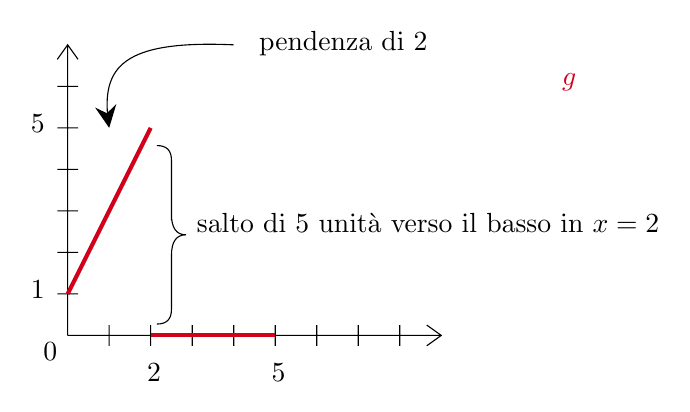
\begin{tikzpicture}[x=0.75pt,y=0.75pt,yscale=-1,xscale=1]
%uncomment if require: \path (0,203); %set diagram left start at 0, and has height of 203

%Shape: Axis 2D [id:dp46013604632113503] 
\draw  (200,160) -- (380,160)(200,20) -- (200,160) -- cycle (373,155) -- (380,160) -- (373,165) (195,27) -- (200,20) -- (205,27) (220,155) -- (220,165)(240,155) -- (240,165)(260,155) -- (260,165)(280,155) -- (280,165)(300,155) -- (300,165)(320,155) -- (320,165)(340,155) -- (340,165)(360,155) -- (360,165)(195,140) -- (205,140)(195,120) -- (205,120)(195,100) -- (205,100)(195,80) -- (205,80)(195,60) -- (205,60)(195,40) -- (205,40) ;
\draw   ;
%Straight Lines [id:da5583914209314376] 
\draw [color={rgb, 255:red, 208; green, 2; blue, 27 }  ,draw opacity=1 ][line width=1.5]    (240,60) -- (200,140) ;
%Straight Lines [id:da8784587512983899] 
\draw [color={rgb, 255:red, 208; green, 2; blue, 27 }  ,draw opacity=1 ][line width=1.5]    (300,160) -- (240,160) ;
%Shape: Brace [id:dp22057370394693132] 
\draw   (243,154.53) .. controls (247.67,154.53) and (250,152.2) .. (250,147.53) -- (250,121.53) .. controls (250,114.86) and (252.33,111.53) .. (257,111.53) .. controls (252.33,111.53) and (250,108.2) .. (250,101.53)(250,104.53) -- (250,75.53) .. controls (250,70.86) and (247.67,68.53) .. (243,68.53) ;
%Curve Lines [id:da9997704212540879] 
\draw    (280,20) .. controls (226.44,17.62) and (216.19,30.57) .. (219.58,57.06) ;
\draw [shift={(220,60)}, rotate = 261.02] [fill={rgb, 255:red, 0; green, 0; blue, 0 }  ][line width=0.08]  [draw opacity=0] (10.72,-5.15) -- (0,0) -- (10.72,5.15) -- (7.12,0) -- cycle    ;

% Text Node
\draw (181,132.4) node [anchor=north west][inner sep=0.75pt]    {$1$};
% Text Node
\draw (181,52.4) node [anchor=north west][inner sep=0.75pt]    {$5$};
% Text Node
\draw (237,172.4) node [anchor=north west][inner sep=0.75pt]    {$2$};
% Text Node
\draw (187,162.4) node [anchor=north west][inner sep=0.75pt]    {$0$};
% Text Node
\draw (297,172.4) node [anchor=north west][inner sep=0.75pt]    {$5$};
% Text Node
\draw (437,32.4) node [anchor=north west][inner sep=0.75pt]  [color={rgb, 255:red, 208; green, 2; blue, 27 }  ,opacity=1 ]  {$g$};
% Text Node
\draw (261,100) node [anchor=north west][inner sep=0.75pt]   [align=left] {salto di $5$ unità verso il basso in $x=2$};
% Text Node
\draw (291,12) node [anchor=north west][inner sep=0.75pt]   [align=left] {pendenza di $2$};


\end{tikzpicture}
\end{figure}
\FloatBarrier

Il salto verso l'alto in $x=0$ non lo possiamo vedere perché le funzioni test sono nulle prima di zero.
\Soluzione
\begin{nb}
Si può dimostrare che se $v\in D'(\mathbb{R})$, $\psi \in C^{\infty }(\mathbb{R}) \Rightarrow \psi v\in D'(\mathbb{R})$ e il suo effetto su una funzione test $\varphi $ è
\begin{equation*}
\langle \psi v,\varphi \rangle :=\langle v,\psi \varphi \rangle 
\end{equation*}
\end{nb}
Quindi
\begin{equation*}
\langle x\delta '_{0} (x),\varphi \rangle =\langle \delta '_{0} (x),x\varphi ( x) \rangle =-\langle \delta _{0} ,x\varphi '( x) +\varphi ( x) \rangle =-\varphi ( 0) =\langle -\delta _{0} ,\varphi \rangle 
\end{equation*}
Cioè in $D'(\mathbb{R})$
\begin{equation*}
x\delta '_{0} =-\delta _{0}
\end{equation*}
\textit{Esercizio per casa.}

$\forall n,m\in \mathbb{N}$ trovare la distribuzione di $u( x) =x^{m} \delta ^{( n)}_{0}$.
\Soluzione
\begin{equation*}
f_{n} (x)=g(x)*\chi _{(0,n)} =\int _{\mathbb{R}} e^{-(x-t)} H(x-t)\chi _{(0,n)} (t)dt=\int ^{n}_{0} e^{-x} e^{t} H(x-t)dt
\end{equation*}
\fg{0.7}{13-3}
\begin{gather*}
\begin{cases}
0, & x< 0\\
\int ^{x}_{0} e^{-x} e^{t} dt, & 0\leqslant x\leqslant n\\
\int ^{n}_{0} e^{-x} e^{t} dt, & x >n
\end{cases} =\begin{cases}
0, & x< 0\\
e^{-x}\left( e^{x} -1\right) =1-e^{-x} & 0\leqslant x\leqslant n\\
e^{-x} (e^{n} -1) & x >n
\end{cases}\\
\\
\xrightarrow{n\rightarrow \infty } F( x) =\begin{cases}
0, & x< 0\\
1-e^{-x} , & x\geqslant 0
\end{cases}
\end{gather*}
\begin{itemize}
\item Convergenza in $L^{p}(\mathbb{R})$?

No perché l'ipotetico limite $F( x)$ non è integrabile a $+\infty $.
\item Convergenza in $L^{\infty }(\mathbb{R})$?

Notiamo che

\begin{equation*}
\begin{aligned}
\Vert F\Vert _{L^{\infty }(\mathbb{R})} & =\sup _{\mathbb{R}}| F( x)| =1\xrightarrow{n\rightarrow +\infty } 1\\
\Vert f_{n}\Vert _{L^{\infty }(\mathbb{R})} & =\sup _{\mathbb{R}}| f_{n}( x)| =1-e^{-n}\xrightarrow{n\rightarrow +\infty } 1
\end{aligned}
\end{equation*}

Tuttavia non possiamo concludere da queste due affermazioni che c'è convergenza in $L^{\infty }$, quello che ci interessa è la \textit{differenza} in norma infinito.

\begin{equation*}
\Vert f_{n} -F\Vert _{L^{\infty }(\mathbb{R})} =\begin{cases}
0, & x< n\\
F( x) -f_{n}( x) , & x\geqslant n
\end{cases} =\begin{cases}
0, & x< n\\
1-e^{n-x} , & x\geqslant n
\end{cases}
\end{equation*}

È un esponenziale traslato di $n$

\begin{equation*}
\Vert f_{n} -F\Vert _{L^{\infty }(\mathbb{R})} =\sup _{\mathbb{R}}| f_{n}( x) -F( x)| =1\nrightarrow 0
\end{equation*}

Quindi non c'è convergenza in $L^{\infty }(\mathbb{R})$.
\item Convergenza in $D'(\mathbb{R})$?

Sono distribuzioni in quanto $f_{n} ,F\in L^{1}_{\mathrm{loc}}(\mathbb{R})$.

\begin{equation*}
\langle f_{n} ,\varphi \rangle \rightarrow \langle F,\varphi \rangle \ \ \forall \varphi \in D(\mathbb{R}) \ \ \Leftrightarrow \ \ \langle F-f_{n} ,\varphi \rangle \rightarrow 0
\end{equation*}

nel nostro caso

\begin{equation*}
\langle F-f_{n} ,\varphi \rangle =\int ^{\infty }_{n}\left( 1-e^{n-x}\right) \varphi (x)dx=0\ \ \forall n\geqslant n_{\varphi }
\end{equation*}

perché $\varphi $ è a supporto compatto, cioè $\forall \varphi \ \exists n_{\varphi } :\varphi ( x) =0,\forall x\geqslant n$. Il dominio di integrazione prima o poi andrà oltre il dominio di $\varphi $, che poi si annullerà.

Quindi

\begin{equation*}
f_{n}\xrightarrow{D'(\mathbb{R} )} F
\end{equation*}
\item Convergenza in $\mathcal{S} '(\mathbb{R} )$?\begin{equation*}
\langle f_{n} ,\psi \rangle \rightarrow \langle F,\psi \rangle \ \ \forall \psi \in S(\mathbb{R}) \ \ \Leftrightarrow \ \ \langle F-f_{n} ,\psi \rangle \rightarrow 0
\end{equation*}

dove $S$ è lo spazio di Schwarz, lo spazio delle funzioni a decrescita rapida\begin{equation*}
\psi \in C^{\infty } \ \ \land \ \ \lim\limits _{x\rightarrow +\infty } x^{n} \psi ( x) =0
\end{equation*}

nel nostro caso

\begin{equation*}
\langle F-f_{n} ,\psi \rangle =\int ^{+\infty }_{n}\left( 1-e^{n-x}\right) \psi ( x) dx=\int ^{+\infty }_{0}\left( 1-e^{n-x}\right) \chi _{( n,+\infty )}( x) \psi ( x) dx
\end{equation*}

Se chiamiamo $h_{n}( x)$ l'integranda

\begin{equation*}
\lim\limits _{n\rightarrow +\infty } h_{n}( x) =0
\end{equation*}

Usiamo la convergenza dominata

\begin{equation*}
| h_{n}( x)| \leqslant | \psi ( x)| \ \ | \psi ( x)| \in L^{1}(\mathbb{R})
\end{equation*}

Allora

\begin{equation*}
\langle F-f_{n} ,\psi \rangle \rightarrow 0
\end{equation*}
\end{itemize}
\Soluzione
\begin{equation*}
f( x) \sim \sum\limits ^{\infty }_{n=1} b_{n}\sin( nx)
\end{equation*}
Calcoliamo i coefficienti
\begin{equation*}
b_{n} =\frac{2}{\pi }\int ^{\pi }_{0} 1\cdotp \sin( nx) dx=\frac{2}{\pi }\left[ -\frac{1}{n}\cos( nx)\right]^{\pi }_{0} =\frac{2}{\pi n}\left( 1-( -1)^{n}\right) =\begin{cases}
\frac{4}{n\pi } , & n\ \text{dispari}\\
0, & n\ \text{pari}
\end{cases}
\end{equation*}
La serie cercata è
\begin{equation*}
f( x) \sim \sum\limits ^{\infty }_{k=0}\frac{4}{( 2k+1) \pi }\sin(( 2k+1) x)
\end{equation*}
Questa funzione è anche una distribuzione? Sì, $f\in L^{1}_{\mathrm{loc}}(\mathbb{R})$.
\begin{equation*}
\langle u,\varphi \rangle =\langle u,\varphi ( x+T) \rangle 
\end{equation*}
In $D'(\mathbb{R})$, a occhio possiamo dedurre la derivata\footnote{Si noti la somiglianza col Pettine di Dirac.}


\begin{figure}[htpb]
	\centering
\tikzset{every picture/.style={line width=0.75pt}} %set default line width to 0.75pt        

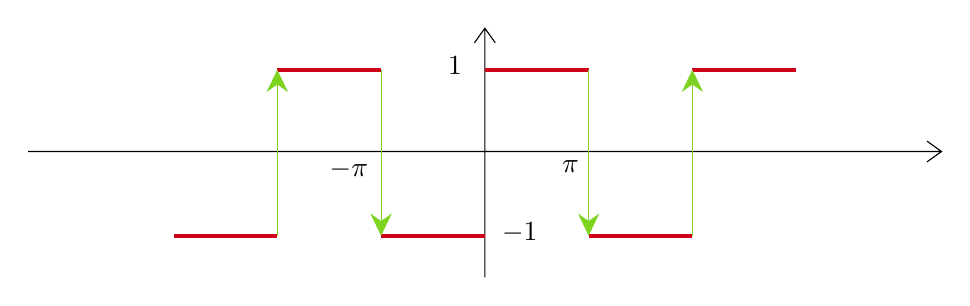
\begin{tikzpicture}[x=0.75pt,y=0.75pt,yscale=-1,xscale=1]
%uncomment if require: \path (0,132); %set diagram left start at 0, and has height of 132

%Shape: Axis 2D [id:dp6130811625741925] 
\draw  (80,69.4) -- (520,69.4)(300,10) -- (300,130) (513,64.4) -- (520,69.4) -- (513,74.4) (295,17) -- (300,10) -- (305,17)  ;
%Straight Lines [id:da4688738915321422] 
\draw [color={rgb, 255:red, 208; green, 2; blue, 27 }  ,draw opacity=1 ][line width=1.5]    (300,30) -- (350,30) ;
%Straight Lines [id:da564644152513289] 
\draw [color={rgb, 255:red, 208; green, 2; blue, 27 }  ,draw opacity=1 ][line width=1.5]    (250,110) -- (300,110) ;
%Straight Lines [id:da1288587788441018] 
\draw [color={rgb, 255:red, 208; green, 2; blue, 27 }  ,draw opacity=1 ][line width=1.5]    (400,30) -- (450,30) ;
%Straight Lines [id:da42001293411482954] 
\draw [color={rgb, 255:red, 208; green, 2; blue, 27 }  ,draw opacity=1 ][line width=1.5]    (350,110) -- (400,110) ;
%Straight Lines [id:da41879142834815575] 
\draw [color={rgb, 255:red, 208; green, 2; blue, 27 }  ,draw opacity=1 ][line width=1.5]    (200,30) -- (250,30) ;
%Straight Lines [id:da34094039721778624] 
\draw [color={rgb, 255:red, 208; green, 2; blue, 27 }  ,draw opacity=1 ][line width=1.5]    (150,110) -- (200,110) ;
%Straight Lines [id:da6751056390959596] 
\draw [color={rgb, 255:red, 126; green, 211; blue, 33 }  ,draw opacity=1 ]   (350,30) -- (350,107) ;
\draw [shift={(350,110)}, rotate = 270] [fill={rgb, 255:red, 126; green, 211; blue, 33 }  ,fill opacity=1 ][line width=0.08]  [draw opacity=0] (10.72,-5.15) -- (0,0) -- (10.72,5.15) -- (7.12,0) -- cycle    ;
%Straight Lines [id:da8152221642203317] 
\draw [color={rgb, 255:red, 126; green, 211; blue, 33 }  ,draw opacity=1 ]   (250,30) -- (250,107) ;
\draw [shift={(250,110)}, rotate = 270] [fill={rgb, 255:red, 126; green, 211; blue, 33 }  ,fill opacity=1 ][line width=0.08]  [draw opacity=0] (10.72,-5.15) -- (0,0) -- (10.72,5.15) -- (7.12,0) -- cycle    ;
%Straight Lines [id:da21495238477473233] 
\draw [color={rgb, 255:red, 126; green, 211; blue, 33 }  ,draw opacity=1 ]   (200,110) -- (200,33) ;
\draw [shift={(200,30)}, rotate = 450] [fill={rgb, 255:red, 126; green, 211; blue, 33 }  ,fill opacity=1 ][line width=0.08]  [draw opacity=0] (10.72,-5.15) -- (0,0) -- (10.72,5.15) -- (7.12,0) -- cycle    ;
%Straight Lines [id:da5779103582115537] 
\draw [color={rgb, 255:red, 126; green, 211; blue, 33 }  ,draw opacity=1 ]   (400,110) -- (400,33) ;
\draw [shift={(400,30)}, rotate = 450] [fill={rgb, 255:red, 126; green, 211; blue, 33 }  ,fill opacity=1 ][line width=0.08]  [draw opacity=0] (10.72,-5.15) -- (0,0) -- (10.72,5.15) -- (7.12,0) -- cycle    ;

% Text Node
\draw (281,22.4) node [anchor=north west][inner sep=0.75pt]    {$1$};
% Text Node
\draw (307,102.4) node [anchor=north west][inner sep=0.75pt]    {$-1$};
% Text Node
\draw (224,72.4) node [anchor=north west][inner sep=0.75pt]    {$-\pi $};
% Text Node
\draw (336,72.4) node [anchor=north west][inner sep=0.75pt]    {$\pi $};


\end{tikzpicture}
\end{figure}
\FloatBarrier

\begin{equation*}
f'( x) =\sum\limits ^{+\infty }_{k=-\infty }( -1)^{k} \cdotp 2\delta _{k\pi }( x)
\end{equation*}
Possiamo derivare termine a termine
\begin{equation*}
f'( x)\overset{D'(\mathbb{R})}{\sim }\sum\limits ^{\infty }_{k=0}\frac{4}{\pi }\cos(( 2k+1) x)
\end{equation*}
\chapter{Esercitazione 7 - Potrich}
\ParteEsercizi
\begin{definition}
[Distribuzione] Una distribuzione è un operatore $u$ che a ogni funzione test $\varphi $ (funzione $C^{\infty }(\mathbb{R})$ il cui supporto è un compatto $\Omega $ contenuto in $\mathbb{R}$) associa un numero, reale o complesso, $\langle u,\varphi \rangle $ chiamato \textbf{dualità} tra $u$ e $\varphi $ tale che:
\begin{equation*}
\begin{array}{ l }
\langle u,a\varphi +b\psi \rangle =a\langle u,\varphi \rangle +b\langle u,\psi \rangle \ \ \forall a,b\in \mathbb{C} ,\ \forall \varphi ,\psi \in D( \Omega )\\
\varphi _{j}\rightarrow \varphi \ \text{in} \ D( \Omega ) \ \ \Rightarrow \ \ \langle u,\varphi _{j} \rangle \rightarrow \langle u,\varphi \rangle 
\end{array}
\end{equation*}
\end{definition}
\begin{oss}
[Delta di Dirac] L'esempio fondamentale di distribuzione in $D'\left(\mathbb{R}^{n}\right)$ è la Delta di Dirac, denotata $\delta $, e così definita
\begin{equation*}
\langle \delta ,\varphi \rangle =\varphi ( 0) \ \ \forall \varphi \in D\left(\mathbb{R}^{n}\right)
\end{equation*}
\end{oss}
\begin{definition}
Se \ $u\in D'(\mathbb{R})$, allora la derivata distribuzionale di $u$ è la distribuzione $u'\in D'(\mathbb{R})$ definita univocamente da
\begin{equation*}
\int _{\mathbb{R}} u'\varphi =-\int _{\mathbb{R}} u\varphi '\ \ \forall \varphi \in D(\mathbb{R})
\end{equation*}
\end{definition}
\begin{definition}
Si definisce prodotto di una distribuzione in $\Omega $ per una funzione $C^{\infty }( \Omega )$: se $\psi \in C^{\infty }( \Omega )$ e $u\in D'(\mathbb{R})$, allora $( \psi u) \in D'( \Omega )$ è la distribuzione tale che
\begin{equation*}
\langle \psi u,\varphi \rangle =\langle u,\psi \varphi \rangle \ \ \forall \varphi \in D\left(\mathbb{R}^{n}\right)
\end{equation*}
\end{definition}
\begin{nb}
\begin{equation*}
\langle u,\varphi \rangle :=\int _{\Omega } u( x) \varphi ( x) dx,\ \ u\in D'( \Omega ) ,\ \varphi \in D( \Omega )
\end{equation*}
\end{nb}
\Esercizio{}

Provare che valgono le seguenti identità in $D'(\mathbb{R})$:
\begin{enumerate}
\item $x\delta ( x) =0$
\item $x\delta '( x) =-\delta ( x)$
\end{enumerate}
\Esercizio{(TDE 6/07/2015)}

Mostrare che, per ogni $n\in \mathbb{N}^{+}$, si ha
\begin{equation*}
\boxed{x^{n} \delta ^{( n)} =( -1)^{n} n!\delta \ \ \text{in} \ D'}
\end{equation*}
\Esercizio{(Teorema di derivazione di funzioni con discontinuità di tipo salto)}

Sia $a\in \mathbb{R}$, $f\in C^{1}(( -\infty ,a))$, $g\in C^{1}(( a,+\infty ))$ con $f'\in L^{1}(( -\infty ,a))$ e $g'\in L^{1}(( a,+\infty ))$ e definiamo
\begin{equation*}
u( x) =\begin{cases}
f( x) , & x< a\\
g( x) , & x >a
\end{cases}
\end{equation*}
allora $u$ risulta definita q.o. su $\mathbb{R}$ e la sua derivata distribuzionale $u'$ è la somma di una funzione localmente integrabile e che coincide con $f'$ in $( -\infty ,a)$ e con $g'$ in $( a,+\infty )$ più una parte singolare, data dalla Delta di Dirac concentrata in $x=a$ e moltiplicata per l'ampiezza del salto
\begin{equation*}
[ u( a_{+}) -u( a_{-})] \delta _{a}
\end{equation*}
\Esercizio{}

Si consideri
\begin{equation*}
f_{n}( x) =\frac{n}{1+n^{2} x^{2}}
\end{equation*}
provare che $f_{n}\rightarrow \pi \delta $ in $\mathcal{S} '(\mathbb{R})$ e in $D'(\mathbb{R})$.
\Esercizio{}

Si considerino
\begin{equation*}
f_{n}( x) =\frac{1}{\sqrt{n}} \chi _{[ 0,n]}( x) \ \ \ \ \ \ \ \ g_{n}( x) =\sin( nx) \chi _{[ 0,7]}( x)
\end{equation*}
Stabilire se le successioni sono convergenti in $L^{1}(\mathbb{R}) ,L^{2}(\mathbb{R}) ,L^{\infty }(\mathbb{R}) ,D'(\mathbb{R}) ,\mathcal{S} '(\mathbb{R})$.
\Esercizio{}

Si consideri
\begin{equation*}
f_{n}( x) =n^{2} xe^{-n| x| }
\end{equation*}
\begin{enumerate}
\item Determinare il limite puntuale
\item Stabilire se $f_{n}$ converge in $L^{p}$, con $p\in [ 1,+\infty ]$
\item Determinare il limite di\begin{equation*}
g_{n}( x) =f_{n}( x) H( x) \ \ \text{in} \ D'(\mathbb{R})
\end{equation*}

dove\begin{equation*}
H( x) =\begin{cases}
1, & x\geqslant 0\\
0, & x< 0
\end{cases}
\end{equation*}

detta \textbf{Funzione di Heaviside}.
\item Determinare il limite di $f_{n}$ in $D'(\mathbb{R})$
\end{enumerate}
\ParteSoluzioni
\Soluzione
\begin{enumerate}
\item $\forall \varphi \in D(\mathbb{R})$\begin{equation*}
\langle x\delta ,\varphi \rangle =\langle \delta ,x\varphi \rangle =0\cdotp \varphi ( 0) =0\qed 
\end{equation*}
\item $\forall \varphi \in D(\mathbb{R})$\begin{gather*}
\begin{aligned}
\langle x\delta ',\varphi \rangle  & =\langle \delta ',x\varphi \rangle =-\langle \delta ,( x\varphi ) '\rangle \\
 & =-\langle \delta ,\varphi +x\varphi '\rangle \\
 & =-\langle \delta ,\varphi \rangle -\langle \delta ,x\varphi '\rangle =-\varphi ( 0)
\end{aligned}\\
\qed 
\end{gather*}
\end{enumerate}
\Soluzione

Per induzione
\begin{itemize}
\item La formula è vera per $n=1$, per l'esercizio precedente\begin{equation*}
x\delta '( x) =-\delta ( x)
\end{equation*}
\item Supponiamo vera la tesi per $n$ generico\begin{equation*}
\langle x^{n} \delta ^{( n)} ,\varphi \rangle =( -1)^{n} n!\langle \delta ,\varphi \rangle \ \ \forall \varphi \in D
\end{equation*}

dobbiamo mostrare che vale anche per $n+1$\begin{gather*}
\begin{aligned}
\langle x^{n+1} \delta ^{( n+1)} ,\varphi \rangle  & =\langle \delta ^{( n+1)} ,x^{n+1} \varphi \rangle =-\langle \delta ^{( n)} ,\left( x^{n+1} \varphi \right) '\rangle \\
 & =-\langle \delta ^{( n)} ,( n+1) x^{n} \varphi +x^{n+1} \varphi '\rangle \\
 & =-\langle x^{n} \delta ^{( n)} ,( n+1) \varphi +x\varphi '\rangle \\
 & \overset{\text{induz.}}{=} -\langle ( -1)^{n} n!\delta ,( n+1) \varphi +x\varphi '\rangle \\
 & =( -1)^{n+1}( n+1) !\langle \delta ,\varphi \rangle \underbrace{-( -1)^{n} n!\langle \delta ,x\varphi '\rangle }_{=0}\\
 & =( -1)^{n+1}( n+1) !\langle \delta ,\varphi \rangle 
\end{aligned}\\
\qed 
\end{gather*}
\end{itemize}
\Soluzione

Per comodità $u( a_{-}) =f( a) :=f( a_{-})$ e $u( a_{+}) =g( a) :=g( a_{+})$.

Questi termini esistono finiti perché $f',g'$ sono integrabili.

$\forall \varphi \in D(\mathbb{R})$
\begin{equation*}
\langle u',\varphi \rangle =-\langle u,\varphi '\rangle =-\int ^{+\infty }_{-\infty } u( x) \varphi '( x) dx
\end{equation*}
la funzione $u$ è definita a tratti
\begin{equation*}
-\int ^{+\infty }_{-\infty } u( x) \varphi '( x) dx=-\int ^{a}_{-\infty } f( x) \varphi '( x) dx-\int ^{+\infty }_{a} g( x) \varphi '( x) dx=( *)
\end{equation*}
integro per parti
\begin{gather*}
\begin{aligned}
( *) & =-[ f( x) \varphi ( x)]^{a}_{-\infty } +\int ^{a}_{-\infty } f'( x) \varphi ( x) dx-[ g( x) \varphi ( x)]^{+\infty }_{a} +\int ^{+\infty }_{a} g'( x) \varphi ( x) dx\\
 & =-f( a) \varphi ( a) +\int ^{a}_{-\infty } f'( x) \varphi ( x) dx+g( a) \varphi ( a) +\int ^{+\infty }_{a} g'( x) \varphi ( x) dx\\
 & =\varphi ( a)[ g( a) -f( a)] +\int ^{a}_{-\infty } f'( x) \varphi ( x) dx+\int ^{+\infty }_{a} g'( x) \varphi ( x) dx\\
 & =[ u( a_{+}) -u( a_{-})] \langle \delta _{x=a} ,\varphi \rangle +\int ^{a}_{-\infty } f'( x) \varphi ( x) dx+\int ^{+\infty }_{a} g'( x) \varphi ( x) dx
\end{aligned}\\
\qed 
\end{gather*}
\textit{Esempio.}
\begin{equation*}
\sgn( x) =\begin{cases}
1, & x >0\\
-1, & x< 0
\end{cases}
\end{equation*}
Per $x >0$, $\sgn '( x) =0$.

Per $x< 0$, $\sgn '( x) =0$.

$\sgn( x)$ presenta un salto in $x=0$ di ampiezza $2$.
\begin{equation*}
\Rightarrow \ \ \sgn '( x) =0+0+2\delta ( x)
\end{equation*}
\textit{Esempio.}
\begin{equation*}
f( x) =\frac{1}{2}\sgn xe^{-| x| } =\begin{cases}
\frac{1}{2} e^{-x} , & x >0\\
-\frac{1}{2} e^{x} , & x< 0
\end{cases}
\end{equation*}
Per $x >0$, $f'( x) =-\frac{1}{2} e^{-x}$.

Per $x< 0$, $f'( x) =-\frac{1}{2} e^{x}$.

$f( x)$ presenta un salto in $x=0$ di ampiezza $1$.
\begin{equation*}
\Rightarrow \ \ f'( x) =-\frac{1}{2} e^{-| x| } +\delta ( x)
\end{equation*}
\Soluzione

\fg{0.45}{14-4}

Se dimostro in $\mathcal{S} '(\mathbb{R})$, quella in $D'(\mathbb{R})$ segue automaticamente.

Devo provare che
\begin{equation*}
\int _{\mathbb{R}}\frac{n\varphi ( x)}{1+n^{2} x^{2}} dx\xrightarrow{n\rightarrow +\infty } \pi \varphi ( 0) \ \ \forall \varphi \in S(\mathbb{R})
\end{equation*}
pongo $nx=t\Rightarrow ndx=dt$
\begin{equation*}
\int _{\mathbb{R}}\frac{n\varphi \left(\frac{t}{n}\right)}{1+t^{2}}\frac{dt}{n} =\int _{\mathbb{R}} \varphi \left(\frac{t}{n}\right)\frac{1}{1+t^{2}} dt
\end{equation*}
Proviamo che tale convergenza ha luogo per ogni $\varphi $ limitata in $0$ stimando la differenza
\begin{equation*}
\left| \int _{\mathbb{R}} \varphi \left(\frac{t}{n}\right)\frac{1}{1+t^{2}} dt-\pi \varphi ( 0)\right| \leqslant \underbrace{\left| \int _{| t| \leqslant T}\frac{\varphi \left(\frac{t}{n}\right) -\varphi ( 0)}{1+t^{2}} dt\right| }_{I_{1}} +\underbrace{\left| \int _{| t|  >T}\frac{\varphi \left(\frac{t}{n}\right) -\varphi ( 0)}{1+t^{2}} dt\right| }_{I_{2}}
\end{equation*}
Per mostrare la convergenza di questi due integrali posso applicare la convergenza dominata
\begin{equation*}
\left| \varphi \left(\frac{t}{n}\right)\frac{1}{1+t^{2}}\right| \leqslant \frac{\Vert \varphi \Vert _{\infty }}{1+t^{2}} \in L^{1}(\mathbb{R})
\end{equation*}
\begin{nb}
\begin{gather*}
\frac{1}{1+t^{2}} \in L^{1}(\mathbb{R}) \ \ \ \ \ \ \ \ \int _{\mathbb{R}}\frac{1}{1+t^{2}} dt=[\arctan t]^{+\infty }_{-\infty } =\frac{\pi }{2} -\left( -\frac{\pi }{2}\right) =\pi \\
\\
\Rightarrow \ \ \forall \varepsilon  >0\ \ \exists T=T( \varepsilon ) :\ \int _{| t|  >T}\frac{1}{1+t^{2}} dt\leqslant \varepsilon 
\end{gather*}
Fissati $\varepsilon ,T,\ \exists n$ tale che
\begin{equation*}
\left| \varphi \left(\frac{t}{n}\right) -\varphi ( 0)\right| \leqslant \varepsilon \ \ \forall t:\ | t| \leqslant T
\end{equation*}
Allora
\begin{equation*}
I_{1} +I_{2} \leqslant \pi \varepsilon +2\Vert \varphi \Vert _{\infty } \varepsilon 
\end{equation*}
Per l'arbitrarietà di $\varepsilon $ segue la tesi.
\end{nb}
\Soluzione

Studiamo le $f_{n}( x)$
\begin{equation*}
| f_{n}( x)| \leqslant \frac{1}{\sqrt{n}} \ \ \forall x\in \mathbb{R} \ \ \Rightarrow \ \ f_{n}\xrightarrow[n\rightarrow +\infty ]{L^{\infty }(\mathbb{R})} f\equiv 0
\end{equation*}
ma allora
\begin{equation*}
f_{n}\xrightarrow[n\rightarrow +\infty ]{L^{1}_{\mathrm{loc}}(\mathbb{R})} f\equiv 0\ \ \begin{cases}
\Rightarrow \ \ f_{n}\xrightarrow[n\rightarrow +\infty ]{D'(\mathbb{R})} f\equiv 0\\
\Rightarrow \ \ f_{n}\xrightarrow[n\rightarrow +\infty ]{\mathcal{S} '(\mathbb{R})} f\equiv 0
\end{cases}
\end{equation*}
Stimiamo
\begin{equation*}
\Vert f_{n} -0\Vert _{L^{1}} =\Vert f_{n}\Vert _{L^{1}} =\frac{n}{\sqrt{n}} =\sqrt{n}\cancel{\xrightarrow{n\rightarrow +\infty }} 0\ \ \Rightarrow \ \ f_{n}\cancel{\xrightarrow[n\rightarrow +\infty ]{L^{1}(\mathbb{R})}} 0
\end{equation*}
Poi
\begin{equation*}
\Vert f_{n} -0\Vert _{L^{2}} =\Vert f_{n}\Vert _{L^{2}} =1\cancel{\xrightarrow{n\rightarrow +\infty }} 0\ \ \Rightarrow \ \ f_{n}\cancel{\xrightarrow[n\rightarrow +\infty ]{L^{2}(\mathbb{R})}} 0
\end{equation*}


Studiamo le $g_{n}( x)$

Dimostro che $g_{n}$ converge in $\mathcal{S} '(\mathbb{R})$, da cui si ottiene che $g_{n}$ converge anche in $D'(\mathbb{R})$.
\begin{equation*}
\int _{\mathbb{R}} g_{n}( x) \varphi ( x) dx=\overset{\text{ipp}}{=} -\frac{1}{n}[\cos( nx) \varphi ( x)]^{7}_{0} +\int ^{7}_{0}\frac{1}{n}\cos( nx) \varphi '( x) dx\xrightarrow{n\rightarrow +\infty } 0
\end{equation*}
Analizziamo in $L^{\infty }$
\begin{equation*}
\Vert g_{n} -g\Vert _{\infty } =\Vert g_{n}\Vert _{\infty } =1\cancel{\xrightarrow{n\rightarrow +\infty }} 0\ \ \Rightarrow \ \ g_{n}\cancel{\xrightarrow[n\rightarrow +\infty ]{L^{\infty }(\mathbb{R})}} 0
\end{equation*}
Analizziamo in $L^{p}$
\begin{equation*}
\Vert g_{n} -g\Vert ^{p}_{L^{p}} =\Vert g_{n}\Vert ^{p}_{L^{p}} =\int ^{7}_{0}| \sin( nx)| ^{p} dx\overset{nx=y}{=}\frac{1}{n}\int ^{7n}_{0}| \sin( y)| ^{p} dy
\end{equation*}
\begin{oss}
$a >0$
\begin{equation*}
a\int ^{ka}_{0}| \sin y| ^{p} dy=\frac{2h\pi }{k}\int ^{2h\pi }_{0}| \sin y| ^{p} dy+\frac{1}{k}\int ^{ka}_{2h\pi }| \sin y| ^{p} dy
\end{equation*}
dove $h=h( k)$ è l'unico intero tale che $2h\pi \leqslant ka\leqslant 2( h+1) \pi $.

Se $k\rightarrow +\infty $ allora $\frac{2h\pi }{k}\rightarrow 1$ e
\begin{equation*}
\int ^{2h\pi }_{0}| \sin y| ^{p} dy=\int ^{2\pi }_{0}| \sin y| ^{p} dy\ \ \forall h
\end{equation*}
mentre l'altro addendo è infinitesimo.
\end{oss}
Quindi
\begin{equation*}
\frac{1}{n}\int ^{7n}_{0}| \sin( y)| ^{p} dy\xrightarrow{n\rightarrow +\infty } 7\int ^{2\pi }_{0}| \sin y| ^{p} dy\ \ \Rightarrow \ \ g_{n}\cancel{\xrightarrow[n\rightarrow +\infty ]{L^{p}(\mathbb{R})}} 0
\end{equation*}
\Soluzione
\begin{enumerate}
\item Fissiamo $x_{0} \in \mathbb{R}$.
\begin{enumerate}
\item se $x_{0} =0$ allora $f_{n}( 0) \equiv 0\ \forall n\in \mathbb{N}$
\item se $x_{0} \neq 0$ allora $\lim\limits _{n\rightarrow +\infty } f_{n}( x_{0}) =0$
\item quindi $f_{n}$ converge puntualmente su tutto $\mathbb{R}$ a $f( x) \equiv 0$.
\end{enumerate}

\fg{0.7}{14-6}
\item Se $p\in [ 1,+\infty )$\begin{equation*}
\Vert f_{n}\Vert ^{p}_{L^{p}} =\int _{\mathbb{R}} n^{2p} x^{p} e^{-np| x| } dx=2\int ^{+\infty }_{0} n^{2p} x^{p} e^{-npx} dx=( *)
\end{equation*}

poniamo $npx=t\Rightarrow npdx=dt$\begin{equation*}
( *) =2\int ^{+\infty }_{0} n^{2p}\frac{t^{p}}{n^{p} p^{p}} e^{-t}\frac{dt}{np} =\frac{2}{p^{p+1}} n^{p-1}\int ^{+\infty }_{0} t^{p} e^{-t} dt\cancel{\xrightarrow{n\rightarrow +\infty }} 0
\end{equation*}

l'integrale non dipende da $n$, siamo nel caso $p\geqslant 1$, quindi non c'è convergenza.

Se $p=\infty $\begin{equation*}
\Vert f_{n} -f\Vert _{\infty } =\Vert f_{n}\Vert _{\infty } =\max_{\mathbb{R}}| f_{n}( x)| =\left| f_{n}\left(\frac{1}{n}\right)\right| =n^{2}\frac{1}{n} e^{-n\frac{1}{n}} =ne^{-1}\cancel{\xrightarrow{n\rightarrow +\infty }} 0
\end{equation*}

quindi non c'è convergenza.
\item La successione $g_{n}$ è\begin{equation*}
g_{n}( x) =f_{n}( x) H( x) =\begin{cases}
n^{2} xe^{-nx} , & x\geqslant 0\\
0, & x< 0
\end{cases}
\end{equation*}

$\forall n\in \mathbb{N} ,\ g_{n} \in L^{1}_{\mathrm{loc}}(\mathbb{R})$ e $\forall \varphi \in D(\mathbb{R})$\begin{equation*}
\langle g_{n} ,\varphi \rangle =\int _{\mathbb{R}} g_{n}( x) \varphi ( x) dx=\int ^{+\infty }_{0} n^{2}\textcolor[rgb]{0.82,0.01,0.11}{x} e^{-nx}\textcolor[rgb]{0.82,0.01,0.11}{\varphi }\textcolor[rgb]{0.82,0.01,0.11}{(}\textcolor[rgb]{0.82,0.01,0.11}{x}\textcolor[rgb]{0.82,0.01,0.11}{)} dx
\end{equation*}

integriamo per parti con\begin{gather*}
\textcolor[rgb]{0.82,0.01,0.11}{f}\textcolor[rgb]{0.82,0.01,0.11}{(}\textcolor[rgb]{0.82,0.01,0.11}{x}\textcolor[rgb]{0.82,0.01,0.11}{)} =x\varphi ( x) \ \ \rightarrow \ \ f'( x) =\varphi ( x) +x\varphi '( x)\\
g( x) =-ne^{-nx} \ \ \rightarrow \ \ g'( x) =n^{2} e^{-nx}
\end{gather*}

da cui\begin{equation*}
\overset{\text{ipp}}{=}\underbrace{\left[ -ne^{-nx} x\varphi ( x)\right]^{+\infty }_{0}}_{=0} +\int ^{+\infty }_{0} ne^{-nx}[\textcolor[rgb]{0.25,0.46,0.02}{\varphi }\textcolor[rgb]{0.25,0.46,0.02}{(}\textcolor[rgb]{0.25,0.46,0.02}{x}\textcolor[rgb]{0.25,0.46,0.02}{)}\textcolor[rgb]{0.25,0.46,0.02}{+x\varphi '}\textcolor[rgb]{0.25,0.46,0.02}{(}\textcolor[rgb]{0.25,0.46,0.02}{x}\textcolor[rgb]{0.25,0.46,0.02}{)}] dx
\end{equation*}

integriamo per parti con\begin{gather*}
\textcolor[rgb]{0.25,0.46,0.02}{f}\textcolor[rgb]{0.25,0.46,0.02}{(}\textcolor[rgb]{0.25,0.46,0.02}{x}\textcolor[rgb]{0.25,0.46,0.02}{)} =\varphi ( x) +x\varphi '( x) \ \ \rightarrow \ \ f'( x) =2\varphi '( x) +x\varphi ''( x)\\
g( x) =-e^{-nx} \ \ \rightarrow \ \ g'( x) =ne^{-nx}
\end{gather*}

da cui\begin{gather*}
\overset{\text{ipp}}{=}\underbrace{\left[ -e^{-nx}( \varphi ( x) +x\varphi '( x))\right]^{+\infty }_{0}}_{\varphi ( 0)} +\int ^{+\infty }_{0} e^{-nx}[ 2\varphi '( x) +x\varphi ''( x)] dx\\
\begin{aligned}
\Rightarrow  & \langle g_{n} ,\varphi \rangle =\varphi ( 0) +\int ^{+\infty }_{0} e^{-nx}[ 2\varphi '( x) +x\varphi ''( x)] dx\\
\Rightarrow  & \lim\limits _{n\rightarrow +\infty } \langle g_{n} ,\varphi \rangle =\varphi ( 0) +\lim\limits _{n\rightarrow +\infty }\int ^{+\infty }_{0} e^{-nx}[ 2\varphi '( x) +x\varphi ''( x)] dx\\
\overset{\text{Dom}}{\Rightarrow } & \lim\limits _{n\rightarrow +\infty } \langle g_{n} ,\varphi \rangle =\varphi ( 0) +\int ^{+\infty }_{0}\lim\limits _{n\rightarrow +\infty } e^{-nx}[ 2\varphi '( x) +x\varphi ''( x)] dx=\varphi ( 0)
\end{aligned}
\end{gather*}

essendo $\varphi \in D(\mathbb{R}) \Rightarrow \exists M >0$ tale che $| 2\varphi '( x) +x\varphi ''( x)| < M,\ \forall x\in \mathbb{R}$ e\begin{equation*}
\left| e^{-nx}[ 2\varphi '( x) +x\varphi ''( x)]\right| \leqslant Me^{-x} \in L^{1}([ 0,+\infty ))
\end{equation*}

quindi\begin{equation*}
g_{n}\xrightarrow[n\rightarrow +\infty ]{D'(\mathbb{R})} \delta _{0}
\end{equation*}
\item $\forall \varphi \in D(\mathbb{R})$\begin{equation*}
\begin{aligned}
\langle f_{n} ,\varphi \rangle  & =\int _{\mathbb{R}} n^{2} xe^{-n| x| } \varphi ( x) dx\\
 & =\int ^{0}_{-\infty } n^{2} xe^{nx} \varphi ( x) dx+\int ^{+\infty }_{0} n^{2} xe^{-nx} \varphi ( x) dx
\end{aligned}
\end{equation*}

integrazione per parti due volte per entrambi gli integrali e teorema della convergenza dominata\begin{align*}
\langle f_{n} ,\varphi \rangle  & =\int _{\mathbb{R}} n^{2} xe^{-n| x| } dx\\
 & =\int ^{0}_{-\infty } n^{2} xe^{nx} \varphi ( x) dx+\int ^{\infty }_{0} n^{2} xe^{-nx} \varphi ( x) dx
\end{align*}

ponendo $f=x\varphi ( x)$ e $g'$ l'altro pezzo per entrambi gli integrali\begin{align*}
 & \overset{\text{ipp}}{=}\cancel{\left[ ne^{nx} \cdotp x\varphi ( x)\right]^{0}_{-\infty }} -\int ^{0}_{-\infty } ne^{nx}[ \varphi ( x) +x\varphi '( x)] dx\\
 & \ \ \ \ +\cancel{\left[ -ne^{-nx} \cdotp x\varphi ( x)\right]^{\infty }_{0}} +\int ^{\infty }_{0} ne^{-nx}[ \varphi ( x) +x\varphi '( x)] dx\\
 & \overset{\text{ipp}}{=} -\left\{\left[ e^{nx} \cdotp ( \varphi ( x) +x\varphi '( x))\right]^{0}_{-\infty } -\int ^{0}_{-\infty } e^{nx}[ \varphi '( x) -\varphi '( x) -x\varphi ''( x)] dx\right\}\\
 & \ \ \ \ +\left\{\left[ -e^{-nx}( \varphi ( x) +x\varphi '( x))\right]^{\infty }_{0} +\int ^{\infty }_{0} e^{-nx}[ \varphi '( x) +\varphi '( x) +x\varphi ''( x)] dx\right\}
\end{align*}

al limite i due integrali si cancellano per convergenza dominata, rimane\begin{equation*}
-[ \varphi ( 0) -0] +[ 0-( -\varphi ( 0))] =-\varphi ( 0) +\varphi ( 0) =-\delta _{0} +\delta _{0} =0
\end{equation*}
\end{enumerate}
\chapter{Esercitazione 8 - Boella}
\ParteEsercizi
\Esercizio{}

Calcolare la trasformata di Fourier di $f(x)=e^{-|x|}$
\Esercizio{}

Calcolare la trasformata di Fourier di $f(x)=\chi _{[-1,1]} (x)$
\Esercizio{}

Calcolare la trasformata di Fourier di $f(x)=e^{-x^{2}}$
\Esercizio{}

Calcolare la trasformata di Fourier di $f(x)=\frac{1}{\cosh (x)}$
\Esercizio{}

Calcolare la trasformata di Fourier di $f(x)=\frac{1}{\left( 1+x^{2}\right)^{2}}$
\Esercizio{}

Calcolare la trasformata di Fourier di $u(x)=\frac{1}{\sqrt{|x|}}$

\ParteSoluzioni
\Soluzione

Grafico di $f( x) =e^{-| x| }$

\fg{0.7}{15-1}
\begin{equation*}
f\ \text{reale pari} \ \ \Rightarrow \ \ \hat{f} \ \text{reale pari}
\end{equation*}
Inoltre $f\in L^{1}(\mathbb{R})$ quindi per il Teorema di Riemann-Lebesgue
\begin{equation*}
f\in L^{1}(\mathbb{R}) \ \ \Rightarrow \ \ \hat{f} \in C^{0}_{0}(\mathbb{R}) \cap L^{\infty }(\mathbb{R})
\end{equation*}
La trasformata di Fourier è derivabile? In $0$ c'è un punto angoloso quindi non possiamo utilizzare la proprietà della trasformata di Fourier per le derivate.

Poiché all'infinito la funzione va a zero come un'esponenziale anche se la moltiplichiamo per una qualsiasi potenza di $x$ quello che otteniamo è ancora una funzione in $L^{1} (\mathbb{R} )$
\begin{equation*}
x^{n} f(x)\in L^{1} (\mathbb{R} )\ \ \Rightarrow \ \ \frac{d^{n}}{d\xi ^{n}}\hat{f} \in C^{0}(\mathbb{R}) \ \ \Rightarrow \ \ \hat{f} \in C^{\infty } (\mathbb{R} )
\end{equation*}
Inoltre
\begin{equation*}
f\notin C^{\infty } (\mathbb{R} )\ \ \Rightarrow \ \ f\notin \mathcal{S}(\mathbb{R}) \ \ \Rightarrow \ \ \hat{f} \notin \mathcal{S}(\mathbb{R})
\end{equation*}
In compenso visto che $f$ è sicuramente una distribuzione temperata anche $\hat{f}$ lo sarà
\begin{equation*}
f\in \mathcal{S} '(\mathbb{R}) \ \ \Rightarrow \ \ \hat{f} \in \mathcal{S} '(\mathbb{R})
\end{equation*}
Inoltre
\begin{equation*}
f\in L^{2}(\mathbb{R}) \cap L^{1}(\mathbb{R}) \ \ \Rightarrow \ \ \hat{f} \in L^{2}(\mathbb{R})
\end{equation*}
Visto che c'è un valore assoluto la cosa migliore da fare è quella di spezzare l'integrale, quindi:
\begin{equation*}
\begin{aligned}
\hat{f} (\xi ) & =\int e^{-i\xi x} \ e^{-|x|} \ dx=\int ^{0}_{-\infty } e^{-i\xi x} \ e^{x} dx+\int ^{+\infty }_{0} e^{-i\xi x} \ e^{-x} dx\\
 & =\left[\frac{1}{1-i\xi } e^{( 1-i\xi ) x}\right]^{0}_{-\infty } +\left[\frac{-1}{1+i\xi } e^{-( 1+i\xi ) x}\right]^{\infty }_{0}\\
 & =\frac{1}{1-i\xi } +\frac{1}{1+i\xi } =\frac{2}{1+\xi ^{2}}
\end{aligned}
\end{equation*}
Ricordiamo la regola
\begin{equation*}
\mathcal{F}\{u(\alpha x)\} =\frac{1}{| \alpha | }\hat{u}\left(\frac{\xi }{\alpha }\right)
\end{equation*}
Sapendo questo, deduciamo quanto vale, dato $\alpha  >0$
\begin{equation*}
\mathcal{F}\left\{e^{-\alpha | x| }\right\} =\frac{1}{\alpha } \cdotp \frac{2}{1+\left(\frac{\xi }{\alpha }\right)^{2}} =\frac{2\alpha }{\alpha ^{2} +\xi ^{2}}
\end{equation*}
Ricordiamo la formula dell'antitrasformata
\begin{equation*}
f( x) =\frac{1}{2\pi }\int _{\mathbb{R}} e^{i\xi x}\left(\frac{2}{1+\xi ^{2}}\right) d\xi =e^{-|x|}
\end{equation*}
Sapendo questo, deduciamo quanto vale
\begin{equation*}
\mathcal{F}\left\{\frac{1}{1+x^{2}}\right\} =\int _{\mathbb{R}} e^{-i\xi x}\left(\frac{1}{1+x^{2}}\right) dx\overset{\text{parità}}{=} \pi e^{-| \xi | }
\end{equation*}
\Soluzione
\begin{equation*}
\begin{aligned}
\hat{f} (\xi ) & =\int _{\mathbb{R}} e^{-i\xi x} \chi _{[-1,1]} dx=\int ^{1}_{-1} e^{-i\xi x} dx=\left[ -\frac{1}{i\xi } e^{-i\xi x}\right]^{1}_{-1} =\\
 & =\frac{1}{i\xi }\left( e^{i\xi } -e^{-i\xi }\right) =\frac{2}{\xi }\frac{e^{i\xi } -e^{-i\xi }}{2i} =\frac{2\sin \xi }{\xi }
\end{aligned}
\end{equation*}
Questa volta $\hat{f} \notin L^{1} (\mathbb{R} )$ ma $\hat{f} \in L^{2} (\mathbb{R} )$

Ragionando come prima
\begin{gather*}
f(x)=\frac{1}{2\pi }\int _{\mathbb{R}} e^{i\xi x}\frac{2\sin( \xi )}{\xi } d\xi \\
\\
\Rightarrow \ \ g( x) =\frac{\sin x}{x} \ \ \Rightarrow \ \ \hat{g}( \xi ) =\pi \chi _{[-1,1]} (\xi )
\end{gather*}
\Soluzione

Abbiamo due diverse
\begin{enumerate}
\item Analisi complessa
\item Equazione differenziale
\end{enumerate}

\textbf{Analisi complessa.}

$f$ reale pari, allora $\hat{f}$ reale pari. Completando il quadrato\footnote{Aggiungiamo e togliamo $\xi ^{2} /4$
\begin{equation*}
-i\xi x-x^{2} =-\left( i\xi x+x^{2}\right) =-\left[\left( x+\frac{i\xi }{2}\right)^{2} +\frac{\xi ^{2}}{4}\right]
\end{equation*}
}
\begin{equation*}
\hat{f} (\xi )=\int _{\mathbb{R}} e^{-i\xi x} e^{-x^{2}} dx=e^{-\frac{\xi ^{2}}{4}}\int _{\mathbb{R}} e^{-\left( x+\frac{i\xi }{2}\right)^{2}} dx
\end{equation*}
Noto che la funzione integranda ha la forma di una gaussiana traslata nel piano complesso, integriamo sul seguente percorso.


\begin{figure}[htpb]
	\centering
\tikzset{every picture/.style={line width=0.75pt}} %set default line width to 0.75pt        

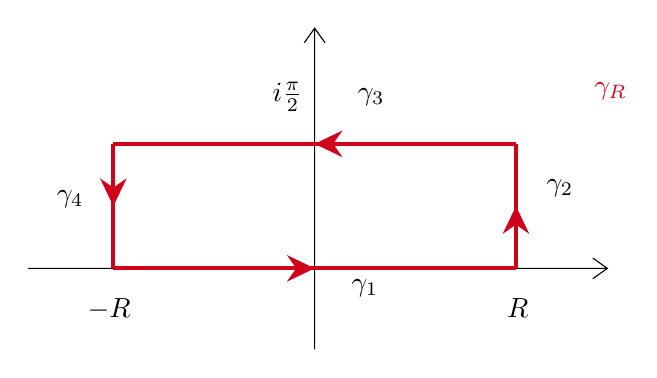
\begin{tikzpicture}[x=0.75pt,y=0.75pt,yscale=-1,xscale=1]
%uncomment if require: \path (0,178); %set diagram left start at 0, and has height of 178

%Shape: Axis 2D [id:dp3537451156705087] 
\draw  (162.5,130.33) -- (441.5,130.33)(300.5,14.63) -- (300.5,169.33) (434.5,125.33) -- (441.5,130.33) -- (434.5,135.33) (295.5,21.63) -- (300.5,14.63) -- (305.5,21.63)  ;
%Straight Lines [id:da6355301965678406] 
\draw [color={rgb, 255:red, 208; green, 2; blue, 27 }  ,draw opacity=1 ][line width=1.5]    (203.5,130.33) -- (397.5,130.33) ;
\draw [shift={(300.5,130.33)}, rotate = 180] [fill={rgb, 255:red, 208; green, 2; blue, 27 }  ,fill opacity=1 ][line width=0.08]  [draw opacity=0] (13.4,-6.43) -- (0,0) -- (13.4,6.44) -- (8.9,0) -- cycle    ;
%Straight Lines [id:da04659866719258687] 
\draw [color={rgb, 255:red, 208; green, 2; blue, 27 }  ,draw opacity=1 ][line width=1.5]    (397.5,70.33) -- (203.5,70.33) ;
\draw [shift={(300.5,70.33)}, rotate = 360] [fill={rgb, 255:red, 208; green, 2; blue, 27 }  ,fill opacity=1 ][line width=0.08]  [draw opacity=0] (13.4,-6.43) -- (0,0) -- (13.4,6.44) -- (8.9,0) -- cycle    ;
%Straight Lines [id:da2855621428556525] 
\draw [color={rgb, 255:red, 208; green, 2; blue, 27 }  ,draw opacity=1 ][line width=1.5]    (397.5,130.33) -- (397.5,70.33) ;
\draw [shift={(397.5,100.33)}, rotate = 450] [fill={rgb, 255:red, 208; green, 2; blue, 27 }  ,fill opacity=1 ][line width=0.08]  [draw opacity=0] (13.4,-6.43) -- (0,0) -- (13.4,6.44) -- (8.9,0) -- cycle    ;
%Straight Lines [id:da09072689237424836] 
\draw [color={rgb, 255:red, 208; green, 2; blue, 27 }  ,draw opacity=1 ][line width=1.5]    (203.5,70.33) -- (203.5,130.33) ;
\draw [shift={(203.5,100.33)}, rotate = 270] [fill={rgb, 255:red, 208; green, 2; blue, 27 }  ,fill opacity=1 ][line width=0.08]  [draw opacity=0] (13.4,-6.43) -- (0,0) -- (13.4,6.44) -- (8.9,0) -- cycle    ;

% Text Node
\draw (392,143.4) node [anchor=north west][inner sep=0.75pt]    {$R$};
% Text Node
\draw (190,143.4) node [anchor=north west][inner sep=0.75pt]    {$-R$};
% Text Node
\draw (279,39.4) node [anchor=north west][inner sep=0.75pt]    {$i\frac{\pi }{2}$};
% Text Node
\draw (434,39.4) node [anchor=north west][inner sep=0.75pt]  [color={rgb, 255:red, 208; green, 2; blue, 27 }  ,opacity=1 ]  {$\gamma _{R}$};
% Text Node
\draw (317,134.4) node [anchor=north west][inner sep=0.75pt]    {$\gamma _{1}$};
% Text Node
\draw (411,86.4) node [anchor=north west][inner sep=0.75pt]    {$\gamma _{2}$};
% Text Node
\draw (320,42.4) node [anchor=north west][inner sep=0.75pt]    {$\gamma _{3}$};
% Text Node
\draw (175,91.4) node [anchor=north west][inner sep=0.75pt]    {$\gamma _{4}$};


\end{tikzpicture}
\end{figure}
\FloatBarrier

La funzione non ha singolarità
\begin{equation*}
\int _{\gamma _{R}} e^{-z^{2}} \ dz=0
\end{equation*}
che è uguale alla somma degli integrali
\begin{equation*}
\int _{\gamma _{R}} e^{-z^{2}} \ dz=\int _{\gamma _{1}} +\int _{\gamma _{2}} +\int _{\gamma _{3}} +\int _{\gamma _{4}}\xrightarrow{R\rightarrow +\infty }\int _{\mathbb{R}} e^{-x^{2}} dx-\int _{\mathbb{R}} e^{-\left( x+\frac{i\xi }{2}\right)^{2}} dx
\end{equation*}
quindi questi due integrali sono uguali al limite
\begin{equation*}
\int _{\mathbb{R}} e^{-\left( x+\frac{i\xi }{2}\right)^{2}} dx=\int _{\mathbb{R}} e^{-x^{2}} dx=\sqrt{\pi }
\end{equation*}
Quindi
\begin{equation*}
\boxed{\mathcal{F}\left\{e^{-x^{2}}\right\} =\sqrt{\pi } e^{-\frac{\xi ^{2}}{4}}}
\end{equation*}
Deduciamo anche, per $\alpha  >0$
\begin{equation*}
\boxed{\mathcal{F}\left\{e^{-\alpha x^{2}}\right\} =\mathcal{F}\left\{e^{-(\sqrt{\alpha } x)^{2}}\right\} =\sqrt{\frac{\pi }{\alpha }} e^{-\frac{\xi ^{2}}{4\alpha }}}
\end{equation*}
\textbf{Equazione differenziale.}

Costruiamo ad hoc un'equazione differenziale
\begin{equation*}
u(x)=e^{-x^{2}} \ \ \Rightarrow \ \ u^{'} (x)=-2xe^{-x^{2}} \ \ \Rightarrow \ \ u^{'} +2xu=0
\end{equation*}
Ora
\begin{equation*}
\mathcal{F}\{u\} =\hat{u} \ \ \ \ \mathcal{F}\{xu\} =i\frac{d}{d\xi }\hat{u} \ \ \ \ \mathcal{F}\{u'\} =i\xi \hat{u} '
\end{equation*}
L'equazione differenziale si riscrive
\begin{equation*}
i\xi \hat{u} +2i\hat{u} '=0\ \ \Rightarrow \ \ \hat{u} '+\frac{\xi }{2}\hat{u} =0\ \ \Rightarrow \ \ \hat{u}( \xi ) =Ce^{-\int \frac{\xi }{2} d\xi } =Ce^{-\xi ^{2} /4}
\end{equation*}
Determiniamo la costante
\begin{equation*}
C=\hat{u}( 0) =\int _{\mathbb{R}} e^{-i0x} u( x) dx=\int _{\mathbb{R}} u( x) dx=\int _{\mathbb{R}} e^{-x^{2}} dx=\sqrt{\pi }
\end{equation*}
Allora
\begin{equation*}
\boxed{\hat{u}( \xi ) =\sqrt{\pi } e^{-\xi ^{2} /4}}
\end{equation*}
\Soluzione

\fg{0.7}{15-4}
\begin{equation*}
\mathcal{F}\left\{\frac{1}{\cosh x}\right\} =\int _{\mathbb{R}}\frac{e^{-i\xi x}}{\cosh x} dx=\int _{\mathbb{R}}\frac{2e^{-i\xi x}}{e^{x} +e^{-x}} dx\ \ \Rightarrow \ \ f( x) =\frac{2e^{-i\xi z}}{e^{z} +e^{-z}}
\end{equation*}
Tutte le singolarità sono tutti i punti del piano complesso in cui si annulla il denominatore 
\begin{equation*}
e^{z} +e^{-z} =e^{-z} (e^{2z} +1)=0\ \ \Leftrightarrow \ \ 2z=i\pi +2k\pi \ \ \Leftrightarrow \ \ z=i\frac{\pi }{2} +k\pi ,\ \ k\in \mathbb{Z}
\end{equation*}
Disegno il grafico con il solito rettangolo della gamma che contenga solo un residuo.


\begin{figure}[htpb]
	\centering
\tikzset{every picture/.style={line width=0.75pt}} %set default line width to 0.75pt        

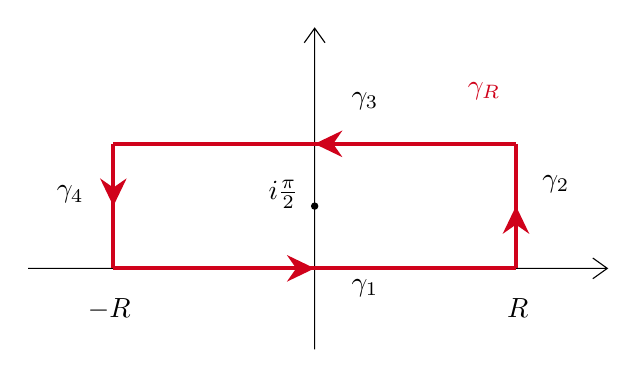
\begin{tikzpicture}[x=0.75pt,y=0.75pt,yscale=-1,xscale=1]
%uncomment if require: \path (0,178); %set diagram left start at 0, and has height of 178

%Shape: Axis 2D [id:dp7510536935747429] 
\draw  (162.5,130.33) -- (441.5,130.33)(300.5,14.63) -- (300.5,169.33) (434.5,125.33) -- (441.5,130.33) -- (434.5,135.33) (295.5,21.63) -- (300.5,14.63) -- (305.5,21.63)  ;
%Straight Lines [id:da06806358271411694] 
\draw [color={rgb, 255:red, 208; green, 2; blue, 27 }  ,draw opacity=1 ][line width=1.5]    (203.5,130.33) -- (397.5,130.33) ;
\draw [shift={(300.5,130.33)}, rotate = 180] [fill={rgb, 255:red, 208; green, 2; blue, 27 }  ,fill opacity=1 ][line width=0.08]  [draw opacity=0] (13.4,-6.43) -- (0,0) -- (13.4,6.44) -- (8.9,0) -- cycle    ;
%Straight Lines [id:da47939213158777694] 
\draw [color={rgb, 255:red, 208; green, 2; blue, 27 }  ,draw opacity=1 ][line width=1.5]    (397.5,70.33) -- (203.5,70.33) ;
\draw [shift={(300.5,70.33)}, rotate = 360] [fill={rgb, 255:red, 208; green, 2; blue, 27 }  ,fill opacity=1 ][line width=0.08]  [draw opacity=0] (13.4,-6.43) -- (0,0) -- (13.4,6.44) -- (8.9,0) -- cycle    ;
%Straight Lines [id:da9055165704816575] 
\draw [color={rgb, 255:red, 208; green, 2; blue, 27 }  ,draw opacity=1 ][line width=1.5]    (397.5,130.33) -- (397.5,70.33) ;
\draw [shift={(397.5,100.33)}, rotate = 450] [fill={rgb, 255:red, 208; green, 2; blue, 27 }  ,fill opacity=1 ][line width=0.08]  [draw opacity=0] (13.4,-6.43) -- (0,0) -- (13.4,6.44) -- (8.9,0) -- cycle    ;
%Straight Lines [id:da5009557145102899] 
\draw [color={rgb, 255:red, 208; green, 2; blue, 27 }  ,draw opacity=1 ][line width=1.5]    (203.5,70.33) -- (203.5,130.33) ;
\draw [shift={(203.5,100.33)}, rotate = 270] [fill={rgb, 255:red, 208; green, 2; blue, 27 }  ,fill opacity=1 ][line width=0.08]  [draw opacity=0] (13.4,-6.43) -- (0,0) -- (13.4,6.44) -- (8.9,0) -- cycle    ;
%Shape: Circle [id:dp4183664382061272] 
\draw  [fill={rgb, 255:red, 0; green, 0; blue, 0 }  ,fill opacity=1 ] (299,100.33) .. controls (299,99.5) and (299.67,98.83) .. (300.5,98.83) .. controls (301.33,98.83) and (302,99.5) .. (302,100.33) .. controls (302,101.16) and (301.33,101.83) .. (300.5,101.83) .. controls (299.67,101.83) and (299,101.16) .. (299,100.33) -- cycle ;

% Text Node
\draw (392,143.4) node [anchor=north west][inner sep=0.75pt]    {$R$};
% Text Node
\draw (190,143.4) node [anchor=north west][inner sep=0.75pt]    {$-R$};
% Text Node
\draw (277,86.4) node [anchor=north west][inner sep=0.75pt]    {$i\frac{\pi }{2}$};
% Text Node
\draw (373,39.4) node [anchor=north west][inner sep=0.75pt]  [color={rgb, 255:red, 208; green, 2; blue, 27 }  ,opacity=1 ]  {$\gamma _{R}$};
% Text Node
\draw (317,134.4) node [anchor=north west][inner sep=0.75pt]    {$\gamma _{1}$};
% Text Node
\draw (409,84.4) node [anchor=north west][inner sep=0.75pt]    {$\gamma _{2}$};
% Text Node
\draw (317,44.4) node [anchor=north west][inner sep=0.75pt]    {$\gamma _{3}$};
% Text Node
\draw (175,89.4) node [anchor=north west][inner sep=0.75pt]    {$\gamma _{4}$};


\end{tikzpicture}
\end{figure}
\FloatBarrier

Calcolo
\begin{equation*}
\begin{aligned}
\int _{\gamma _{R}} f(z)dz & =2\pi i\cdotp \mathrm{Res}\left( f,z=\frac{i\pi }{2}\right) =2\pi i\left. \frac{2e^{-i\xi z}}{e^{z} -e^{-z}}\right| _{z=i\pi /2}\\
 & =2\pi i\cdotp \frac{2e^{\xi \frac{\pi }{2}}}{e^{\frac{i\pi }{2}} -e^{-\frac{i\pi }{2}}} =2\pi i\cdotp \frac{2e^{\xi \frac{\pi }{2}}}{i-( -i)} =2\pi e^{\xi \frac{\pi }{2}}
\end{aligned}
\end{equation*}
Scriviamo i vari pezzi
\begin{align*}
\int _{\gamma _{R}} f( z) dz & =2\pi e^{\frac{\xi \pi }{2}} =\int _{\gamma _{1}} +\int _{\gamma _{2}} +\int _{\gamma _{3}} +\int _{\gamma _{4}}\\
 & \\
\int _{\gamma _{1}} & =\int ^{R}_{-R}\frac{e^{-i\xi x}}{\cosh (x)} dx\xrightarrow{R\rightarrow +\infty }\mathcal{F}\left\{\frac{1}{\cosh (x)}\right\}\\
 & \\
\int _{\gamma _{2}} & =2\int ^{\pi i}_{0}\frac{e^{-i\xi (R+iy)}}{e^{R+iy} +e^{-R-iy}} idy\\
\left| \int _{\gamma _{2}}\right|  & =2\left| \int ^{\pi }_{0}\frac{e^{-i\xi R} e^{y}}{e^{R}\left( e^{iy} +e^{-2R-iy}\right)} idy\right| \leqslant \frac{2}{e^{R}}\underbrace{\int ^{\pi }_{0}\left| \frac{e^{y}}{e^{iy} +e^{-2R-iy}}\right| dy}_{\text{limitata}}\xrightarrow{R\rightarrow +\infty } 0\\
 & \\
\int _{\gamma _{3}} = & -\int ^{R}_{-R}\frac{2e^{-i\xi ( x+i\pi )}}{e^{x+i\pi } +e^{-x-i\pi }} dx=\int ^{R}_{-R}\frac{2e^{-i\xi x} e^{\pi \xi }}{e^{x} +e^{-x}} dx\\
 & =e^{\pi \xi }\int ^{R}_{-R}\frac{e^{-i\xi x}}{\frac{e^{x} +e^{-x}}{2}} dx\xrightarrow{R\rightarrow +\infty } e^{\pi \xi }\mathcal{F}\left\{\frac{1}{\cosh (x)}\right\}\\
 & \\
\left| \int _{\gamma _{4}}\right|  & \xrightarrow{R\rightarrow +\infty } 0
\end{align*}
In totale avremo
\begin{equation*}
2\pi e^{\xi \frac{\pi }{2}} =\int _{\gamma _{R}} f( z) dz\xrightarrow{R\rightarrow +\infty }\mathcal{F}\left\{\frac{1}{\cosh (x)}\right\}\left( 1+e^{\pi \xi }\right)
\end{equation*}
Dunque
\begin{equation*}
\mathcal{F}\left\{\frac{1}{\cosh (x)}\right\} =\frac{2\pi e^{\xi \frac{\pi }{2}}}{e^{\pi \xi } +1} =\frac{2\pi }{e^{\xi \frac{\pi }{2}} +e^{-\xi \frac{\pi }{2}}} =\frac{\pi }{\cosh\left(\frac{\pi }{2} \xi \right)}
\end{equation*}
\Soluzione

\fg{0.7}{15-5}
\begin{equation*}
\mathcal{F}\left\{\frac{1}{\left( 1+x^{2}\right)^{2}}\right\} =\int _{\mathbb{R}}\frac{e^{-i\xi x}}{\left( 1+x^{2}\right)^{2}} dx
\end{equation*}
$f$ pari, allora $\hat{f}$ pari.

Poniamo\footnote{Con $f$ si indica sia la funzione data che quella integranda, ma sono due funzioni che differiscono per il numeratore. Non facciamo troppo i pignoli.}
\begin{equation*}
f( z) =\frac{e^{-i\xi z}}{\left( 1+z^{2}\right)^{2}}
\end{equation*}
$z=\pm i$ sono poli del II ordine.

Giochiamo con i residui utilizzando il Lemma di Jordan
\begin{equation*}
\int _{\gamma _{R}} g( z) e^{i\alpha z} dz
\end{equation*}
\textit{Quale circonferenza bisogna prendere?}

Se $\alpha $ è positivo il lemma di Jordan parla della semicirconferenza superiore mentre se $\alpha $ è negativo della semicirconferenza inferiore.

Nel nostro caso si parla di $-\xi $ per calcolare quanto vale questa trasformata avremo che se $\xi $ è negativo avremo bisogno del semipiano superiore, se $\xi $ è positivo di quello inferiore. Essendo simmetrici si sfrutta il risultato teorico della parità.


\begin{figure}[htpb]
	\centering
\tikzset{every picture/.style={line width=0.75pt}} %set default line width to 0.75pt        

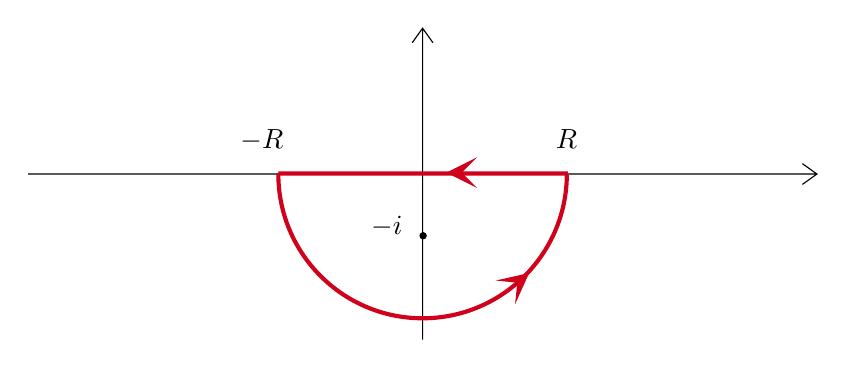
\begin{tikzpicture}[x=0.75pt,y=0.75pt,yscale=-1,xscale=1]
%uncomment if require: \path (0,172); %set diagram left start at 0, and has height of 172

%Shape: Axis 2D [id:dp752436124621402] 
\draw  (110,80.25) -- (490,80.25)(300,10) -- (300,160) (483,75.25) -- (490,80.25) -- (483,85.25) (295,17) -- (300,10) -- (305,17)  ;
%Shape: Arc [id:dp579891374669032] 
\draw  [draw opacity=0][line width=1.5]  (369.5,80.77) .. controls (369.22,118.92) and (338.21,149.75) .. (300,149.75) .. controls (261.62,149.75) and (230.5,118.63) .. (230.5,80.25) .. controls (230.5,80.16) and (230.5,80.07) .. (230.5,79.98) -- (300,80.25) -- cycle ; \draw  [color={rgb, 255:red, 208; green, 2; blue, 27 }  ,draw opacity=1 ][line width=1.5]  (369.5,80.77) .. controls (369.22,118.92) and (338.21,149.75) .. (300,149.75) .. controls (261.62,149.75) and (230.5,118.63) .. (230.5,80.25) .. controls (230.5,80.16) and (230.5,80.07) .. (230.5,79.98) ;
%Shape: Circle [id:dp9196698365325671] 
\draw  [fill={rgb, 255:red, 0; green, 0; blue, 0 }  ,fill opacity=1 ] (298.75,109.99) .. controls (298.75,109.16) and (299.42,108.49) .. (300.25,108.49) .. controls (301.08,108.49) and (301.75,109.16) .. (301.75,109.99) .. controls (301.75,110.82) and (301.08,111.49) .. (300.25,111.49) .. controls (299.42,111.49) and (298.75,110.82) .. (298.75,109.99) -- cycle ;
\draw  [draw opacity=0][fill={rgb, 255:red, 208; green, 2; blue, 27 }  ,fill opacity=1 ] (326.2,86.94) -- (311.45,79.56) -- (326.2,72.19) -- (318.83,79.56) -- cycle ;
\draw  [draw opacity=0][fill={rgb, 255:red, 208; green, 2; blue, 27 }  ,fill opacity=1 ] (335.24,131.55) -- (351.34,127.96) -- (344.55,143) -- (345.62,132.62) -- cycle ;
%Straight Lines [id:da3950283299762536] 
\draw [color={rgb, 255:red, 208; green, 2; blue, 27 }  ,draw opacity=1 ][line width=1.5]    (230.5,79.98) -- (370,80) ;

% Text Node
\draw (211,57.4) node [anchor=north west][inner sep=0.75pt]    {$-R$};
% Text Node
\draw (363,57.4) node [anchor=north west][inner sep=0.75pt]    {$R$};
% Text Node
\draw (274,99.4) node [anchor=north west][inner sep=0.75pt]  [font=\normalsize]  {$-i$};


\end{tikzpicture}
\end{figure}
\FloatBarrier

Per $\xi  >0$
\begin{equation*}
\int _{R}\frac{e^{-i\xi x}}{\left( 1+x^{2}\right)^{2}} dx=-2\pi i\cdotp \mathrm{Res}( f,z=-i)
\end{equation*}
Il segno meno è giustificato dal fatto che percorriamo la semicirconferenza in senso \textit{antiorario}.

Il residuo allora sarà pari a
\begin{equation*}
\begin{aligned}
\mathrm{Res}( f,z=-i) & =\left. \frac{d}{dz}\frac{e^{-i\xi z}}{( z-i)^{2}}\right| _{z=-i}\\
 & =\left. \frac{-i\xi e^{-i\xi z}( z-i)^{2} -e^{-i\xi z} 2(z-i)}{( z-i)^{4}}\right| _{z=-i}\\
 & =\frac{e^{-\xi }( 4i+4i\xi )}{16} =i\frac{e^{-\xi }}{4} (1+\xi )
\end{aligned}
\end{equation*}
La trasformata vale quindi
\begin{equation*}
\mathcal{F}\left\{\frac{1}{\left( 1+x^{2}\right)^{2}}\right\} =-2\pi i\cdotp i\frac{e^{-\xi }}{4} (1+\xi )=\frac{\pi }{2} e^{-\xi }( 1+\xi ) \ \ \ \ \xi  >0
\end{equation*}
Per le $\xi < 0$ basta raddoppiare
\begin{equation*}
\hat{f}( \xi ) =\frac{\pi }{2} e^{-| \xi | } (1+| \xi | )
\end{equation*}
\Soluzione

Vediamo il grafico di $u(x)=1/\sqrt{|x|}$

\fg{0.7}{15-6}

Notiamo che $u\notin L^{1}$ perché all'infinito va a zero troppo lentamente e neanche $u\notin L^{2}$, in tal caso sarebbe asintotica a $1/x$ per $x\rightarrow \infty $, che non è integrabile.

Possiamo considerare $u$ come una distribuzione temperata, cioè $u\in \mathcal{S}^{'}(\mathbb{R})$.

Possiamo prendere una successione di funzioni $u_{n}$ che l'approssimano nel senso delle distribuzioni temperate
\begin{equation*}
u_{n}( x) =u( x) \chi _{( -n,n)}( x) \ \ \ \ u_{n} \in L^{1} (\mathbb{R} )
\end{equation*}
Considerando la dualità con una qualsiasi funzione dello spazio di Schwartz questa sarà pari a:
\begin{gather*}
\langle ( u-u_{n}) ,\psi \rangle =\int ^{-n}_{-\infty }\frac{1}{\sqrt{| x| }} \psi ( x) dx+\ \int ^{+\infty }_{n}\frac{1}{\sqrt{x}} \psi ( x) dx\\
\\
| \langle ( u-u_{n}) ,\ \psi \rangle | \leqslant \frac{1}{\sqrt{n}} \ \int _{\mathbb{R}}| \psi ( x)| dx\xrightarrow{n\rightarrow \infty } 0\ \ \Rightarrow \ \ u_{n}\xrightarrow[\mathcal{S} ']{n\rightarrow \infty } u
\end{gather*}
Ne consegue che possiamo scrivere:
\begin{equation*}
\mathcal{F}\{u\} =\lim _{n\rightarrow \infty }\mathcal{F}\{u_{n}\}
\end{equation*}
Calcoliamo le trasformate delle $u_{n}$ in senso classico
\begin{equation*}
\mathcal{F}\{u_{n}\} =\int _{\mathbb{R}}\frac{e^{-i\xi x}}{\sqrt{|} x|} \chi _{[-n,n]} (u)dx=\int ^{n}_{-n}\frac{\cos( \xi x) -i\sin (\xi x)}{\sqrt{| x| }} dx=2\int ^{n}_{0}\frac{\cos( \xi x)}{\sqrt{x}} dx
\end{equation*}
Sostituzione
\begin{equation*}
\xi x=t^{2} \ \ \Rightarrow \ \ dx=\frac{2}{\xi } tdt
\end{equation*}
Allora
\begin{equation*}
=2\int ^{\sqrt{\xi n}}_{0}\frac{\cos\left( t^{2}\right)}{\sqrt{\frac{t^{2}}{\xi }}}\frac{2t}{\xi } dt=\frac{4}{\sqrt{\xi }} \ \int ^{\sqrt{\xi n}}_{0}\cos\left( t^{2}\right) dt=
\end{equation*}
Ricordiamo l'integrale di Fresnel
\begin{equation*}
\int ^{+\infty }_{0}\cos\left( x^{2}\right) dx=\sqrt{\frac{\pi }{8}}
\end{equation*}
Quindi, la trasformata sarà pari a
\begin{equation*}
\mathcal{F}\{u\} =\lim _{n\rightarrow \infty }\mathcal{F}\{u_{n}\} =\lim _{n\rightarrow \infty }\frac{4}{\sqrt{| \xi | }} \ \int ^{\sqrt{| \xi | n}}_{0}\cos\left( t^{2}\right) dt=\frac{4}{\sqrt{| \xi | }} \ \sqrt{\frac{\pi }{8}} =\ \sqrt{\frac{2\pi }{| \xi | }}
\end{equation*}
\chapter{Esercitazione 8 - Potrich}
\ParteEsercizi
\begin{definition}
Sia $u\in L^{1}(\mathbb{R})$. Si dice \textbf{Trasformata di Fourier} di $u$ la funzione $\hat{u} :\mathbb{R}\rightarrow \mathbb{C}$ definita da
\begin{equation*}
\hat{u}( \xi ) =\int _{\mathbb{R}} e^{-i\xi x} u( x) dx
\end{equation*}
\end{definition}
\begin{theorem}
[Proprietà] Ecco alcune utili proprietà della trasformata di Fourier.
\begin{itemize}
\item Scaling\begin{equation*}
u( ax) \ \ \rightarrow \ \ \frac{1}{| a| }\hat{u}\left(\frac{\xi }{a}\right)
\end{equation*}
\item Shifting\begin{equation*}
u( x-a) \ \ \rightarrow \ \ e^{-ia\xi }\hat{u}( \xi )
\end{equation*}
\item Modulazione\begin{gather*}
u( x) e^{iax} \ \ \rightarrow \ \ \hat{u}( \xi -a)\\
u( x)\cos( \xi _{0} x) \ \ \rightarrow \ \ \frac{1}{2}[\hat{u}( \xi -\xi _{0}) +\hat{u}( \xi +\xi _{0})]
\end{gather*}
\item Linearità\begin{equation*}
\mathcal{F}\{\alpha u+\beta v\} =\alpha \mathcal{F}\{u\} +\beta \mathcal{F}\{v\} \ \ \forall \alpha ,\beta \in \mathbb{R} ,\ \forall u,v\in L^{1}(\mathbb{R})
\end{equation*}
\item Derivazione\begin{equation*}
\widehat{u'}( \xi ) =i\xi \hat{u}( \xi )
\end{equation*}
\end{itemize}
\end{theorem}
\Esercizio{Una trasformata notevole}

Calcolare la trasformata di Fourier di
\begin{equation*}
u( x) =\frac{1}{1+x^{2}} ,\ \ x\in \mathbb{R}
\end{equation*}
\Esercizio{Trasformata della Gaussiana}

Calcolare la trasformata di Fourier della funzione Gaussiana
\begin{equation*}
u( x) =e^{-x^{2}} ,\ x\in \mathbb{R}
\end{equation*}
\Esercizio{}

Calcolare la trasformata di Fourier di
\begin{equation*}
f( x) =\frac{\sin x}{\left( 1+x^{2}\right)\left( 4+x^{2}\right)}
\end{equation*}
\Esercizio{}

Calcolare la trasformata di Fourier di\begin{equation*}
u( x) =\frac{2\cos x}{1+x^{2}}
\end{equation*}
\Esercizio{}

Determinare l'espressione analitica di
\begin{equation*}
f( \tau ) =\int _{\mathbb{R}} e^{-i\left( \tau ^{2} -2\right) x}\frac{\cos( 2x)}{1+x^{2}} dx
\end{equation*}
\Esercizio{}

Sia
\begin{equation*}
f( x) =\begin{cases}
1, & 0< x< 1\\
-1, & -1< x< 0
\end{cases}
\end{equation*}
\begin{enumerate}
\item Calcolare la trasformata di Fourier di $f( x)$
\item Calcolare la trasformata di Fourier di $g( x) =xf( x)$
\end{enumerate}
\Esercizio{}

Sia $H$ la funzione di Heaviside
\begin{equation*}
H( t) =\begin{cases}
1, & t\geqslant 0\\
0, & t< 0
\end{cases}
\end{equation*}
\begin{enumerate}
\item Calcolare la trasformata di Fourier di\begin{equation*}
f( x) =\left( 1-x^{2}\right) H\left( 1-x^{2}\right)
\end{equation*}
\item Utilizzare il risultato trovato per calcolare\begin{equation*}
\int ^{+\infty }_{0}\frac{x\cos x-\sin x}{x^{3}}\cos\left(\frac{x}{2}\right) dx
\end{equation*}
\end{enumerate}
\ParteSoluzioni
\Soluzione

Per definizione
\begin{equation*}
\hat{u}( \xi ) =\int _{\mathbb{R}} e^{-i\xi x} u( x) dx
\end{equation*}
Consideriamo la funzione analitica
\begin{equation*}
f( z) =\frac{1}{1+z^{2}}
\end{equation*}
le cui singolarità si trovano in
\begin{equation*}
1+z^{2} =0\ \ \Leftrightarrow \ \ z=\pm i
\end{equation*}
e sono dei poli semplici.


\begin{figure}[htpb]
	\centering
\tikzset{every picture/.style={line width=0.75pt}} %set default line width to 0.75pt        

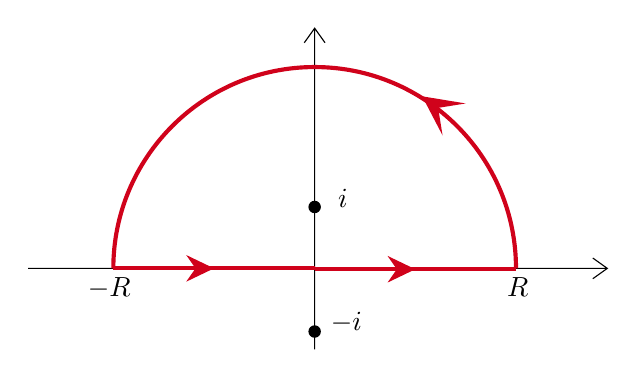
\begin{tikzpicture}[x=0.75pt,y=0.75pt,yscale=-1,xscale=1]
%uncomment if require: \path (0,181); %set diagram left start at 0, and has height of 181

%Shape: Axis 2D [id:dp6994241881147589] 
\draw  (162.5,130.33) -- (441.5,130.33)(300.5,14.63) -- (300.5,169.33) (434.5,125.33) -- (441.5,130.33) -- (434.5,135.33) (295.5,21.63) -- (300.5,14.63) -- (305.5,21.63)  ;
%Straight Lines [id:da47956119812522835] 
\draw [color={rgb, 255:red, 208; green, 2; blue, 27 }  ,draw opacity=1 ][line width=1.5]    (300.5,130.75) -- (397.5,130.75) ;
\draw [shift={(349,130.75)}, rotate = 180] [fill={rgb, 255:red, 208; green, 2; blue, 27 }  ,fill opacity=1 ][line width=0.08]  [draw opacity=0] (13.4,-6.43) -- (0,0) -- (13.4,6.44) -- (8.9,0) -- cycle    ;
%Shape: Arc [id:dp5355059210550983] 
\draw  [draw opacity=0][line width=1.5]  (203.5,130.33) .. controls (203.5,76.76) and (246.93,33.33) .. (300.5,33.33) .. controls (354.07,33.33) and (397.5,76.76) .. (397.5,130.33) -- (300.5,130.33) -- cycle ; \draw  [color={rgb, 255:red, 208; green, 2; blue, 27 }  ,draw opacity=1 ][line width=1.5]  (203.5,130.33) .. controls (203.5,76.76) and (246.93,33.33) .. (300.5,33.33) .. controls (354.07,33.33) and (397.5,76.76) .. (397.5,130.33) ;
%Straight Lines [id:da2269425139728658] 
\draw [color={rgb, 255:red, 208; green, 2; blue, 27 }  ,draw opacity=1 ][line width=1.5]    (203.5,130.33) -- (300.5,130.33) ;
\draw [shift={(252,130.33)}, rotate = 180] [fill={rgb, 255:red, 208; green, 2; blue, 27 }  ,fill opacity=1 ][line width=0.08]  [draw opacity=0] (13.4,-6.43) -- (0,0) -- (13.4,6.44) -- (8.9,0) -- cycle    ;
\draw  [draw opacity=0][fill={rgb, 255:red, 208; green, 2; blue, 27 }  ,fill opacity=1 ] (362.12,66.27) -- (352.31,47.43) -- (373.27,50.88) -- (360,53) -- cycle ;
%Shape: Circle [id:dp54653528391848] 
\draw  [draw opacity=0][fill={rgb, 255:red, 0; green, 0; blue, 0 }  ,fill opacity=1 ] (297.5,100.75) .. controls (297.5,99.1) and (298.84,97.75) .. (300.5,97.75) .. controls (302.16,97.75) and (303.5,99.1) .. (303.5,100.75) .. controls (303.5,102.41) and (302.16,103.75) .. (300.5,103.75) .. controls (298.84,103.75) and (297.5,102.41) .. (297.5,100.75) -- cycle ;
%Shape: Circle [id:dp23929766105583639] 
\draw  [draw opacity=0][fill={rgb, 255:red, 0; green, 0; blue, 0 }  ,fill opacity=1 ] (297.5,160.75) .. controls (297.5,159.1) and (298.84,157.75) .. (300.5,157.75) .. controls (302.16,157.75) and (303.5,159.1) .. (303.5,160.75) .. controls (303.5,162.41) and (302.16,163.75) .. (300.5,163.75) .. controls (298.84,163.75) and (297.5,162.41) .. (297.5,160.75) -- cycle ;

% Text Node
\draw (392,133.4) node [anchor=north west][inner sep=0.75pt]    {$R$};
% Text Node
\draw (190,133.4) node [anchor=north west][inner sep=0.75pt]    {$-R$};
% Text Node
\draw (310.5,90.9) node [anchor=north west][inner sep=0.75pt]    {$i$};
% Text Node
\draw (307,150.4) node [anchor=north west][inner sep=0.75pt]    {$-i$};


\end{tikzpicture}
\end{figure}
\FloatBarrier

Osserviamo che $| f( z)| \sim \frac{1}{z^{2}}$ per $| z| \rightarrow +\infty $, allora col teorema dei residui e il lemma di Jordan
\begin{equation*}
\int ^{+\infty }_{-\infty } e^{-i\xi x}\frac{1}{1+x^{2}} dx=2\pi i\cdotp \mathrm{Res}\left(\frac{e^{-i\xi z}}{1+z^{2}} ,z=i\right) =\pi e^{\xi } \ \ \forall \xi < 0
\end{equation*}
\begin{nb}
Se $f$ è pari, allora $\hat{f}$ è pari.
\end{nb}
I valori per $\xi  >0$ si ottengono da quelli negativi imponendo che $\hat{f}$ sia pari
\begin{nb}
$f\in L^{1} \Rightarrow \hat{f}$ è continua.
\end{nb}
Il valore in $0$ si ottiene per continuità.
\begin{equation*}
\Rightarrow \ \ \boxed{\hat{f}( \xi ) =\pi e^{-| \xi | } \ \ \forall \xi \in \mathbb{R}}
\end{equation*}
\Soluzione
\begin{equation*}
\hat{u}( \xi ) =\int _{\mathbb{R}} e^{-i\xi x} u( x) dx=\int _{\mathbb{R}} e^{-i\xi x} e^{-x^{2}} dx
\end{equation*}
\textbf{\underline{Metodo con l'analisi complessa}}
\begin{equation*}
\hat{u}( \xi ) =\int _{\mathbb{R}} e^{-i\xi x} e^{-x^{2}} dx=\int _{\mathbb{R}} e^{-\left( i\xi x+x^{2}\right)} dx
\end{equation*}
Completiamo il quadrato
\begin{equation*}
\int _{\mathbb{R}} e^{-\left( i\xi x+x^{2}\right)} dx=e^{-\frac{\xi ^{2}}{4}}\int _{\mathbb{R}} e^{-\left( x+\frac{i\xi }{2}\right)^{2}} dx
\end{equation*}
Sfruttiamo la seguente uguaglianza
\begin{equation*}
\int ^{+\infty }_{-\infty } e^{-( x+ib)^{2}} dx\overset{( *)}{=}\int ^{+\infty }_{-\infty } e^{-x^{2}} dx=\sqrt{\pi } \ \ \Rightarrow \ \ \boxed{\hat{u}( \xi ) =\sqrt{\pi } e^{-\frac{\xi ^{2}}{4}}}
\end{equation*}
Resta da provare $( *)$. Consideriamo la funzione analitica intera (senza singolarità) $z\mapsto e^{-z^{2}}$, prolungamento analitico di $e^{-x^{2}} ,x\in \mathbb{R}$.


\begin{figure}[htpb]
	\centering
\tikzset{every picture/.style={line width=0.75pt}} %set default line width to 0.75pt        

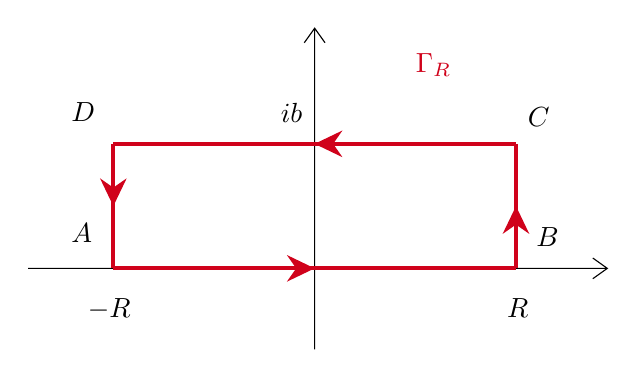
\begin{tikzpicture}[x=0.75pt,y=0.75pt,yscale=-1,xscale=1]
%uncomment if require: \path (0,178); %set diagram left start at 0, and has height of 178

%Shape: Axis 2D [id:dp08896652720756437] 
\draw  (162.5,130.33) -- (441.5,130.33)(300.5,14.63) -- (300.5,169.33) (434.5,125.33) -- (441.5,130.33) -- (434.5,135.33) (295.5,21.63) -- (300.5,14.63) -- (305.5,21.63)  ;
%Straight Lines [id:da3929751532760877] 
\draw [color={rgb, 255:red, 208; green, 2; blue, 27 }  ,draw opacity=1 ][line width=1.5]    (203.5,130.33) -- (397.5,130.33) ;
\draw [shift={(300.5,130.33)}, rotate = 180] [fill={rgb, 255:red, 208; green, 2; blue, 27 }  ,fill opacity=1 ][line width=0.08]  [draw opacity=0] (13.4,-6.43) -- (0,0) -- (13.4,6.44) -- (8.9,0) -- cycle    ;
%Straight Lines [id:da9171312565843239] 
\draw [color={rgb, 255:red, 208; green, 2; blue, 27 }  ,draw opacity=1 ][line width=1.5]    (397.5,70.33) -- (203.5,70.33) ;
\draw [shift={(300.5,70.33)}, rotate = 360] [fill={rgb, 255:red, 208; green, 2; blue, 27 }  ,fill opacity=1 ][line width=0.08]  [draw opacity=0] (13.4,-6.43) -- (0,0) -- (13.4,6.44) -- (8.9,0) -- cycle    ;
%Straight Lines [id:da891206314069279] 
\draw [color={rgb, 255:red, 208; green, 2; blue, 27 }  ,draw opacity=1 ][line width=1.5]    (397.5,130.33) -- (397.5,70.33) ;
\draw [shift={(397.5,100.33)}, rotate = 450] [fill={rgb, 255:red, 208; green, 2; blue, 27 }  ,fill opacity=1 ][line width=0.08]  [draw opacity=0] (13.4,-6.43) -- (0,0) -- (13.4,6.44) -- (8.9,0) -- cycle    ;
%Straight Lines [id:da5821046363194966] 
\draw [color={rgb, 255:red, 208; green, 2; blue, 27 }  ,draw opacity=1 ][line width=1.5]    (203.5,70.33) -- (203.5,130.33) ;
\draw [shift={(203.5,100.33)}, rotate = 270] [fill={rgb, 255:red, 208; green, 2; blue, 27 }  ,fill opacity=1 ][line width=0.08]  [draw opacity=0] (13.4,-6.43) -- (0,0) -- (13.4,6.44) -- (8.9,0) -- cycle    ;

% Text Node
\draw (392,143.4) node [anchor=north west][inner sep=0.75pt]    {$R$};
% Text Node
\draw (190,143.4) node [anchor=north west][inner sep=0.75pt]    {$-R$};
% Text Node
\draw (182,107.4) node [anchor=north west][inner sep=0.75pt]    {$A$};
% Text Node
\draw (182,49.4) node [anchor=north west][inner sep=0.75pt]    {$D$};
% Text Node
\draw (402,51.4) node [anchor=north west][inner sep=0.75pt]    {$C$};
% Text Node
\draw (406,109.4) node [anchor=north west][inner sep=0.75pt]    {$B$};
% Text Node
\draw (283,49.4) node [anchor=north west][inner sep=0.75pt]    {$ib$};
% Text Node
\draw (348,25.4) node [anchor=north west][inner sep=0.75pt]  [color={rgb, 255:red, 208; green, 2; blue, 27 }  ,opacity=1 ]  {$\Gamma _{R}$};


\end{tikzpicture}
\end{figure}
\FloatBarrier

con
\begin{equation*}
\begin{aligned}
A & =-R\\
B & =R\\
C & =R+ib\\
D & =-R+ib
\end{aligned} \ \ \ \ \forall R >0,\forall b >0
\end{equation*}
Per il teorema dell'integrale nullo di Cauchy
\begin{equation*}
\oint _{\Gamma _{R}} e^{-z^{2}} dz=0
\end{equation*}
Sul pezzo $BC$ affermiamo
\begin{equation*}
\lim\limits _{R\rightarrow +\infty }\int ^{C}_{B} e^{-z^{2}} dz=0
\end{equation*}
dato che se $R >2b$ si ottiene, per ogni $z\in BC$,
\begin{gather*}
z=| z| (\cos \vartheta +i\sin \vartheta )\\
\left| e^{-z^{2}}\right| =e^{\mathrm{Re}\left( -z^{2}\right)} =e^{-| z| ^{2}\cos 2\vartheta } \leqslant e^{-R^{2}\cos 2\vartheta } =e^{-R^{2}\left(\cos^{2} \vartheta -\sin^{2} \vartheta \right)} \leqslant e^{-\frac{R^{2}}{4}}\xrightarrow{R\rightarrow +\infty } 0
\end{gather*}
Analogamente
\begin{equation*}
\lim\limits _{R\rightarrow +\infty }\int ^{A}_{D} e^{-z^{2}} dz=0
\end{equation*}
Allora possiamo dire
\begin{equation*}
\Rightarrow \ \ \int ^{B}_{A} e^{-z^{2}} dz=-\int ^{D}_{C} e^{-z^{2}} dz+o\left(\frac{1}{R}\right)
\end{equation*}
Passando al limite per $R\rightarrow +\infty $ si ottiene $( *)$.



\underline{\textbf{Metodo alternativo con equazioni differenziali.}}

Consideriamo l'equazione differenziale lineare omogenea del primo ordine
\begin{equation*}
u'( x) =-2xu( x) ,\ \ x\in \mathbb{R}
\end{equation*}
in quanto $e^{-x^{2}}$ è soluzione di questa equazione differenziale. Andiamo a trasformare tutti i termini di questa equazione.
\begin{equation*}
i\xi \hat{u}( \xi ) =-2i\hat{u} '( \xi ) \ \ \Rightarrow \ \ \hat{u}( \xi ) =Ce^{-\frac{\xi ^{2}}{4}}
\end{equation*}
per cui si deve scegliere
\begin{equation*}
C=\hat{u}( 0) =\int _{\mathbb{R}} e^{-i\xi x} e^{-t^{2}} dt\overset{\xi =0}{=}\int _{\mathbb{R}} e^{-t^{2}} dt=\sqrt{\pi }
\end{equation*}
Concludiamo che
\begin{equation*}
\boxed{\hat{u}( \xi ) =\sqrt{\pi } e^{-\frac{\xi ^{2}}{4}}}
\end{equation*}
\Soluzione

Poniamo
\begin{gather*}
u( x) =\frac{1}{\left( 1+x^{2}\right)\left( 4+x^{2}\right)}\\
\Rightarrow \ \ \hat{u}( \xi ) =\int _{\mathbb{R}} e^{-i\xi x} u( x) dx=\int ^{+\infty }_{-\infty }\frac{e^{-i\xi x}}{\left( 1+x^{2}\right)\left( 4+x^{2}\right)}
\end{gather*}
Poniamo
\begin{equation*}
u( z) =\frac{1}{\left( 1+z^{2}\right)\left( 4+z^{2}\right)} \in \mathcal{H}(\mathbb{C} \setminus \{\pm i,\pm 2i\})
\end{equation*}
Le singolarità sono poli semplici.


\begin{figure}[htpb]
	\centering
\tikzset{every picture/.style={line width=0.75pt}} %set default line width to 0.75pt        

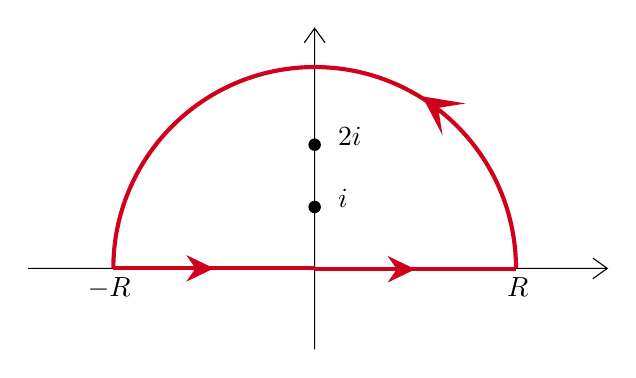
\begin{tikzpicture}[x=0.75pt,y=0.75pt,yscale=-1,xscale=1]
%uncomment if require: \path (0,181); %set diagram left start at 0, and has height of 181

%Shape: Axis 2D [id:dp663384449293001] 
\draw  (162.5,130.33) -- (441.5,130.33)(300.5,14.63) -- (300.5,169.33) (434.5,125.33) -- (441.5,130.33) -- (434.5,135.33) (295.5,21.63) -- (300.5,14.63) -- (305.5,21.63)  ;
%Straight Lines [id:da95452190554064] 
\draw [color={rgb, 255:red, 208; green, 2; blue, 27 }  ,draw opacity=1 ][line width=1.5]    (300.5,130.75) -- (397.5,130.75) ;
\draw [shift={(349,130.75)}, rotate = 180] [fill={rgb, 255:red, 208; green, 2; blue, 27 }  ,fill opacity=1 ][line width=0.08]  [draw opacity=0] (13.4,-6.43) -- (0,0) -- (13.4,6.44) -- (8.9,0) -- cycle    ;
%Shape: Arc [id:dp42287292414644995] 
\draw  [draw opacity=0][line width=1.5]  (203.5,130.33) .. controls (203.5,76.76) and (246.93,33.33) .. (300.5,33.33) .. controls (354.07,33.33) and (397.5,76.76) .. (397.5,130.33) -- (300.5,130.33) -- cycle ; \draw  [color={rgb, 255:red, 208; green, 2; blue, 27 }  ,draw opacity=1 ][line width=1.5]  (203.5,130.33) .. controls (203.5,76.76) and (246.93,33.33) .. (300.5,33.33) .. controls (354.07,33.33) and (397.5,76.76) .. (397.5,130.33) ;
%Straight Lines [id:da4448454277513003] 
\draw [color={rgb, 255:red, 208; green, 2; blue, 27 }  ,draw opacity=1 ][line width=1.5]    (203.5,130.33) -- (300.5,130.33) ;
\draw [shift={(252,130.33)}, rotate = 180] [fill={rgb, 255:red, 208; green, 2; blue, 27 }  ,fill opacity=1 ][line width=0.08]  [draw opacity=0] (13.4,-6.43) -- (0,0) -- (13.4,6.44) -- (8.9,0) -- cycle    ;
\draw  [draw opacity=0][fill={rgb, 255:red, 208; green, 2; blue, 27 }  ,fill opacity=1 ] (362.12,66.27) -- (352.31,47.43) -- (373.27,50.88) -- (360,53) -- cycle ;
%Shape: Circle [id:dp1636459542824935] 
\draw  [draw opacity=0][fill={rgb, 255:red, 0; green, 0; blue, 0 }  ,fill opacity=1 ] (297.5,100.75) .. controls (297.5,99.1) and (298.84,97.75) .. (300.5,97.75) .. controls (302.16,97.75) and (303.5,99.1) .. (303.5,100.75) .. controls (303.5,102.41) and (302.16,103.75) .. (300.5,103.75) .. controls (298.84,103.75) and (297.5,102.41) .. (297.5,100.75) -- cycle ;
%Shape: Circle [id:dp3693616304321441] 
\draw  [draw opacity=0][fill={rgb, 255:red, 0; green, 0; blue, 0 }  ,fill opacity=1 ] (297.5,70.75) .. controls (297.5,69.1) and (298.84,67.75) .. (300.5,67.75) .. controls (302.16,67.75) and (303.5,69.1) .. (303.5,70.75) .. controls (303.5,72.41) and (302.16,73.75) .. (300.5,73.75) .. controls (298.84,73.75) and (297.5,72.41) .. (297.5,70.75) -- cycle ;

% Text Node
\draw (392,133.4) node [anchor=north west][inner sep=0.75pt]    {$R$};
% Text Node
\draw (190,133.4) node [anchor=north west][inner sep=0.75pt]    {$-R$};
% Text Node
\draw (310.5,90.9) node [anchor=north west][inner sep=0.75pt]    {$i$};
% Text Node
\draw (310.5,60.9) node [anchor=north west][inner sep=0.75pt]    {$2i$};


\end{tikzpicture}
\end{figure}
\FloatBarrier

Notiamo che $| u( z)| \sim \frac{1}{z^{4}}$ per $| z| \rightarrow +\infty $. Per il teorema dei residui e il lemma di Jordan
\begin{equation*}
\begin{aligned}
\hat{u}( \xi ) & =\int ^{+\infty }_{-\infty }\frac{e^{-i\xi x}}{\left( 1+x^{2}\right)\left( 4+x^{2}\right)}\overset{\xi < 0}{=} 2\pi i\cdotp \{\mathrm{Res}( u,i) +\mathrm{Res}( u,2i)\}\\
 & =2\pi i\cdotp \left\{\frac{e^{\xi }}{6i} -\frac{e^{2\xi }}{12i}\right\} =\frac{\pi }{3} e^{\xi } -\frac{\pi }{6} e^{2\xi } \ \ ( \xi < 0)
\end{aligned}
\end{equation*}
$u( x)$ è pari, allora $\hat{u}( \xi )$ è pari e reale.

$\Rightarrow $ i valori per $\xi  >0$ si ottengono imponendo $\hat{u}( -\xi ) =\hat{u}( \xi )$.

$u\in L^{1}(\mathbb{R})$, allora la sua trasformata è continua.

$\Rightarrow $ il valore per $\xi =0$ si ottiene per continuità.
\begin{equation*}
\hat{u}( \xi ) =\frac{\pi }{3} e^{-| \xi | } -\frac{\pi }{6} e^{-2| \xi | } \ \ \ \ \forall \xi \in \mathbb{R}
\end{equation*}
A questo punto ricordiamo la proprietà della \textit{modulazione}
\begin{equation*}
u( x) e^{iax} \mapsto \hat{u}( \xi -a)
\end{equation*}
e che possiamo scrivere le identità
\begin{equation*}
\cos \vartheta =\frac{e^{i\vartheta } +e^{-i\vartheta }}{2} \ \ \ \ \sin \vartheta =\frac{e^{i\vartheta } -e^{-i\vartheta }}{2i}
\end{equation*}
in modo da far apparire il termine per usare la proprietà
\begin{equation*}
\begin{aligned}
\mathcal{F}( f( x) ,\xi ) & =\mathcal{F}\left(\frac{\sin x}{\left( 1+x^{2}\right)\left( 4+x^{2}\right)} ,\xi \right)\\
 & =\mathcal{F}\left(\frac{e^{ix} -e^{-ix}}{2i\left( 1+x^{2}\right)\left( 4+x^{2}\right)} ,\xi \right)\\
 & =\frac{1}{2i}\mathcal{F}\left(\frac{e^{ix}}{\left( 1+x^{2}\right)\left( 4+x^{2}\right)} ,\xi \right) +\frac{1}{2i}\mathcal{F}\left(\frac{-e^{-ix}}{\left( 1+x^{2}\right)\left( 4+x^{2}\right)} ,\xi \right)\\
 & =\frac{1}{2i}\left\{\mathcal{F}\left(\frac{1}{\left( 1+x^{2}\right)\left( 4+x^{2}\right)} ,\xi -1\right) -\mathcal{F}\left(\frac{1}{\left( 1+x^{2}\right)\left( 4+x^{2}\right)} ,\xi +1\right)\right\}\\
 & =\frac{1}{2i}\left\{\frac{\pi }{3} e^{-| \xi -1| } -\frac{\pi }{6} e^{-2| \xi -1| } -\frac{\pi }{3} e^{-| \xi +1| } +\frac{\pi }{6} e^{-2| \xi +1| }\right\}
\end{aligned}
\end{equation*}
\Soluzione

Conviene riscrivere $u$
\begin{equation*}
u( x) =\frac{2\cos x}{1+x^{2}} =u( x) =\frac{2\frac{e^{ix} +e^{-ix}}{2}}{1+x^{2}} =\frac{e^{ix} +e^{-ix}}{1+x^{2}}
\end{equation*}
Sappiamo dal primo esercizio che
\begin{equation*}
\mathcal{F}\left\{\frac{1}{1+x^{2}} ,\xi \right\} =\pi e^{-| \xi | }
\end{equation*}
Allora
\begin{equation*}
\begin{aligned}
\mathcal{F}\{u( x) ,\xi \} & =\mathcal{F}\left\{\frac{e^{ix} +e^{-ix}}{1+x^{2}} ,\xi \right\}\\
 & =\mathcal{F}\left\{\frac{e^{ix}}{1+x^{2}} ,\xi \right\} +\mathcal{F}\left\{\frac{e^{-ix}}{1+x^{2}} ,\xi \right\}\\
 & =\pi e^{-| \xi -1| } +\pi e^{-| \xi +1| }
\end{aligned}
\end{equation*}
\Soluzione

Posto
\begin{equation*}
g( x) =\frac{\cos( 2x)}{1+x^{2}}
\end{equation*}
Per definizione
\begin{equation*}
\hat{g}( \xi ) =\int _{\mathbb{R}} e^{-i\xi x} g( x) dx
\end{equation*}
e dunque
\begin{equation*}
f( \tau ) =\hat{g}\left( \tau ^{2} -2\right)
\end{equation*}
Sappiamo per il primo esercizio che
\begin{equation*}
\mathcal{F}\left\{\frac{1}{1+x^{2}} ,\xi \right\} =\pi e^{-| \xi | }
\end{equation*}
Inoltre
\begin{equation*}
g( x) =\frac{\cos( 2x)}{1+x^{2}} =\frac{e^{2ix} +e^{-2ix}}{2\left( 1+x^{2}\right)}
\end{equation*}
Allora
\begin{equation*}
\hat{g}( \xi ) =\mathcal{F}\{g( x) ,\xi \} =\frac{\pi }{2}\left( e^{-| \xi -2| } +e^{-| \xi +2| }\right)
\end{equation*}
E determiniamo $f( \tau )$ come
\begin{equation*}
f( \tau ) =\hat{g}\left( \tau ^{2} -2\right) =\frac{\pi }{2}\left( e^{-\left| \tau ^{2} -4\right| } +e^{-\left| \tau ^{2}\right| }\right)
\end{equation*}
\Soluzione
\begin{enumerate}
\item Calcoliamo\begin{equation*}
\begin{aligned}
\hat{f}( \xi ) & =\int _{\mathbb{R}} e^{-i\xi x} f( x) dx\\
 & =\int ^{0}_{-1} -e^{-i\xi x} dx+\int ^{1}_{0} e^{-i\xi x} dx\\
 & =\left[\frac{1}{i\xi } e^{-i\xi x}\right]^{0}_{-1} +\left[ -\frac{1}{i\xi } e^{-i\xi x}\right]^{1}_{0}\\
 & =\frac{1}{i\xi }\left( 1-e^{i\xi } -e^{-i\xi } +1\right)\\
 & =\frac{1}{i\xi }\left( 2-\textcolor[rgb]{0.29,0.56,0.89}{\left(e^{i\xi }+e^{-i\xi }\right)}\right) =\frac{1}{i\xi }( 2-\textcolor[rgb]{0.29,0.56,0.89}{2\cos\xi })
\end{aligned}
\end{equation*}
\item Calcoliamo\begin{equation*}
\hat{g}( \xi ) =i\frac{d}{d\xi }\hat{f}( \xi ) =i\frac{d}{d\xi }\frac{2-2\cos \xi }{i\xi } =\frac{2( 1-\cos \xi -\xi \sin \xi )}{\xi ^{2}}
\end{equation*}
\end{enumerate}
\Soluzione

$f$ può essere riscritta
\begin{equation*}
f( x) =\begin{cases}
1-x^{2} , & -1\leqslant x\leqslant 1\\
0, & \text{altrove}
\end{cases}
\end{equation*}
$f$ è pari, allora $\hat{f}$ è pari e reale.
\begin{equation*}
\hat{f}( \xi ) =\int _{\mathbb{R}} e^{-i\xi x} f( x) dx=\int ^{1}_{-1} e^{-i\xi x}\left( 1-x^{2}\right) dx=( *)
\end{equation*}
Usando l'analisi complessa
\begin{equation*}
\rho e^{i\vartheta } =\rho [\cos \vartheta +i\sin \vartheta ]
\end{equation*}
allora
\begin{align*}
( *) & =\int ^{1}_{-1}[\cos( \xi x) -i\sin( \xi x)]\left( 1-x^{2}\right) dx\\
 & =\int ^{1}_{-1}\underbrace{\cos( \xi x)\left( 1-x^{2}\right)}_{\text{pari}} dx-i\int ^{1}_{-1}\underbrace{\sin( \xi x)\left( 1-x^{2}\right)}_{\text{dispari}} dx\\
 & =2\int ^{1}_{0}\underbrace{\cos( \xi x)}_{g'}\underbrace{\left( 1-x^{2}\right)}_{f} -i\cdotp 0\\
 & \overset{\text{ipp}}{=} 2\left\{\cancel{\left[\left( 1-x^{2}\right)\frac{1}{\xi }\sin( 2\xi )\right]^{1}_{0}} -\int ^{1}_{0}\frac{-2x}{\xi }\sin( \xi x) dx\right\}\\
 & =\frac{4}{\xi }\int ^{1}_{0}\underbrace{x}_{f}\underbrace{\sin( \xi x)}_{g'} dx\\
 & \overset{\text{ipp}}{=}\frac{4}{\xi }\left\{\left[ -\frac{x}{\xi }\cos( \xi x)\right]^{1}_{0} -\int ^{1}_{0} -\frac{1}{\xi }\cos( \xi x) dx\right\}\\
 & =\frac{4}{\xi }\left\{-\frac{1}{\xi }\cos \xi +\left[\frac{1}{\xi ^{2}}\sin( \xi x)\right]^{1}_{0}\right\}\\
 & =\frac{4}{\xi }\left\{-\frac{1}{\xi }\cos \xi +\frac{1}{\xi ^{2}}\sin( \xi )\right\}\\
 & =-\frac{4}{\xi ^{2}}\cos \xi +\frac{4}{\xi ^{3}}\sin \xi =4\left(\frac{\sin \xi -\xi \cos \xi }{\xi ^{3}}\right)
\end{align*}
\begin{theorem}
[Antitrasformata di Fourier] Siano $u,\hat{u} \in L^{1}(\mathbb{R})$
\begin{equation*}
\boxed{u( x) =\frac{1}{2\pi }\int _{\mathbb{R}} e^{i\xi x}\hat{u}( \xi ) d\xi \ \ \forall x\in \mathbb{R}}
\end{equation*}
\end{theorem}
Allora, ricordando che $\hat{f}$ è pari
\begin{align*}
f( x) & =\frac{1}{2\pi }\int _{\mathbb{R}} e^{i\xi x}\hat{f}( \xi ) d\xi \\
 & =\frac{1}{2\pi }\int _{\mathbb{R}}[\cos( \xi x) +i\sin( \xi x)]\hat{f}( \xi ) \xi \\
 & =\frac{1}{2\pi }\int _{\mathbb{R}}\cos( \xi x) \cdotp \hat{f}( \xi ) d\xi \\
 & =\frac{1}{2\pi } \cdotp 2\int ^{\infty }_{0}\cos( \xi x) \cdotp \hat{f}( \xi ) d\xi \\
 & =\frac{1}{2\pi } \cdotp 2\int ^{\infty }_{0}\cos( \xi x) \cdotp 4\left(\frac{\sin \xi -\xi \cos \xi }{\xi ^{3}}\right) d\xi \\
 & =\frac{4}{\pi }\int ^{+\infty }_{0}\frac{\sin \xi -\xi \cos \xi }{\xi ^{3}}\cos( \xi x) d\xi 
\end{align*}
Per avere l'integrale richiesto dobbiamo prendere $x=\frac{1}{2}$
\begin{equation*}
f\left(\frac{1}{2}\right) =\frac{4}{\pi }\int ^{+\infty }_{0}\frac{\sin \xi -\xi \cos \xi }{\xi ^{3}}\cos\left(\frac{\xi }{2}\right) d\xi \ \ \ \ \ \ \ \ f\left(\frac{1}{2}\right) =1-\frac{1}{4} =\frac{3}{4}
\end{equation*}
Troviamo quindi il l'integrale richiesto, a meno di un segno
\begin{equation*}
\int ^{+\infty }_{0}\frac{x\cos x-\sin x}{x^{3}}\cos\left(\frac{x}{2}\right) dx=-\frac{3}{4} \cdotp \frac{\pi }{4} =-\frac{3\pi }{16}
\end{equation*}
\chapter{Esercitazione 9 - Boella}
\ParteEsercizi

Richiami di teoria sulla Trasformata di Laplace.
\begin{definition}
[Funzione di Heaviside] Si definisce
\begin{equation*}
H( t) =\begin{cases}
1, & t\geqslant 0\\
0, & t< 0
\end{cases}
\end{equation*}
\end{definition}
\begin{figure}[htpb]
	\centering
\tikzset{every picture/.style={line width=0.75pt}} %set default line width to 0.75pt        

\begin{tikzpicture}[x=0.75pt,y=0.75pt,yscale=-1,xscale=1]
%uncomment if require: \path (0,158); %set diagram left start at 0, and has height of 158

%Shape: Axis 2D [id:dp10122351594887924] 
\draw  (150.5,120) -- (448.5,120)(299.5,15) -- (299.5,152) (441.5,115) -- (448.5,120) -- (441.5,125) (294.5,22) -- (299.5,15) -- (304.5,22)  ;
%Straight Lines [id:da9543821452612189] 
\draw [line width=1.5]    (142.5,120) -- (296.15,120) ;
\draw [shift={(299.5,120)}, rotate = 0] [color={rgb, 255:red, 0; green, 0; blue, 0 }  ][line width=1.5]      (0, 0) circle [x radius= 4.36, y radius= 4.36]   ;
%Straight Lines [id:da289644330277681] 
\draw [line width=1.5]    (429.5,80) -- (299.5,80) ;
\draw [shift={(299.5,80)}, rotate = 180] [color={rgb, 255:red, 0; green, 0; blue, 0 }  ][fill={rgb, 255:red, 0; green, 0; blue, 0 }  ][line width=1.5]      (0, 0) circle [x radius= 4.36, y radius= 4.36]   ;

% Text Node
\draw (281,68.4) node [anchor=north west][inner sep=0.75pt]    {$1$};
% Text Node
\draw (282,125.4) node [anchor=north west][inner sep=0.75pt]    {$0$};
% Text Node
\draw (452,122.4) node [anchor=north west][inner sep=0.75pt]    {$t$};


\end{tikzpicture}
\end{figure}
\FloatBarrier
Diciamo che $\mathcal{L}\{f( t)\} =F( s)$.

\textbf{Alcune trasformate notevoli.}
\begin{itemize}
\item $\mathcal{L}\{H( t)\} =\int ^{+\infty }_{0} e^{-st} dt=\frac{1}{s}$, in questo caso $\lambda =0$
\item $\mathcal{L}\left\{t^{k} f( t)\right\} =( -1)^{k}\frac{d^{k}}{ds^{k}} F( s)$
\item $\mathcal{L}\{tH( t)\} =\frac{1}{s^{2}}$

$\mathcal{L}\left\{t^{2} H( t)\right\} =-\left( -\frac{2}{s^{3}}\right) =\frac{2}{s^{3}}$

$\mathcal{L}\left\{t^{3} H( t)\right\} =-\frac{d}{ds}\left(\frac{2}{s^{3}}\right) =\frac{6}{s^{4}}$

$\mathcal{L}\left\{t^{n} H( t)\right\} =\frac{n!}{s^{n+1}}$
\item $\Gamma ( x) =\int ^{+\infty }_{0} t^{x-1} e^{-t} dt$
\begin{itemize}
\item $\Gamma ( n) =( n-1) !$ se $n$ è intero
\item $\Gamma ( x+1) =x\Gamma ( x)$ per ogni $x >0$
\item $\Gamma \left(\frac{1}{2}\right) =\sqrt{\pi }$
\end{itemize}

$\mathcal{L}\left\{t^{\alpha } H( t)\right\} =\frac{\Gamma ( \alpha +1)}{s^{\alpha +1}}$ se $\mathrm{Re}( \alpha )  >-1$
\item $\mathcal{L}\left\{\frac{1}{\sqrt{t}} H( t)\right\} =\frac{\Gamma \left(\frac{1}{2}\right)}{\sqrt{s}} =\frac{\sqrt{\pi }}{\sqrt{s}}$
\end{itemize}

\textbf{Proprietà.}
\begin{itemize}
\item $\mathcal{L}\{f( \alpha t)\} =\frac{1}{\alpha } F\left(\frac{s}{\alpha }\right)$
\item $\mathcal{L}\{f( t-\alpha )\} =e^{-\alpha s} F( s)$
\item $\mathcal{L}\left\{e^{\alpha t} f( t)\right\} =F( s-\alpha )$
\item $\mathcal{L}\{f'( t)\} =sF( s) -f\left( 0^{+}\right)$
\item $\mathcal{L}\{f''( t)\} =s^{2} F( s) -sf\left( 0^{+}\right) -f'\left( 0^{+}\right)$
\item $\mathcal{L}\left\{\int ^{t}_{0} f( \tau ) d\tau \right\} =\frac{1}{s} F( s)$
\item $\mathcal{L}\left\{\frac{1}{t} f( t)\right\} =\int ^{+\infty }_{s} F( \sigma ) d\sigma $
\end{itemize}

\textbf{Altre trasformate notevoli.}
\begin{itemize}
\item $\mathcal{L}\left\{e^{\alpha t} H( t)\right\} =\frac{1}{s-\alpha }$
\item $\mathcal{L}\{\sin( \omega t) H( t)\} =\frac{\omega }{s^{2} +\omega ^{2}}$, pari in $s$
\item $\mathcal{L}\{\cos( \omega t) H( t)\} =\frac{s}{s^{2} +\omega ^{2}}$, dispari in $s$
\item $\mathcal{L}\{\sinh( \omega t) H( t)\} =\frac{\omega }{s^{2} -\omega ^{2}}$
\item $\mathcal{L}\{\cosh( \omega t) H( t)\} =\frac{s}{s^{2} -\omega ^{2}}$
\end{itemize}
\Esercizio{}

Calcolare
\begin{equation*}
\mathcal{L}\left\{e^{-\alpha t}\sin( \omega t) H( t)\right\} =\frac{\omega }{\omega ^{2} +( s+\alpha )^{2}}
\end{equation*}
Calcolare
\begin{equation*}
\begin{aligned}
\mathcal{L}\left\{e^{-t}\sin^{2}( t) H( t)\right\} & =\frac{1}{2}\mathcal{L}\left\{e^{-t}( 1-\cos 2t) H( t)\right\} =\frac{1}{2}\left[\frac{1}{s+1} -\frac{s+1}{4+( s+1)^{2}}\right]\\
 & =\frac{1}{2}\frac{4}{( s+1)\left( 4+( s+1)^{2}\right)} =\frac{2}{( s+1)\left( 4+( s+1)^{2}\right)}
\end{aligned}
\end{equation*}
Calcolare
\begin{equation*}
\mathcal{L}\left\{\int ^{t}_{0}\sin( 2\tau ) d\tau \right\} =\frac{2}{s\left( 4+s^{2}\right)}
\end{equation*}
Calcolare
\begin{equation*}
\begin{aligned}
\mathcal{L}\left\{t^{2} e^{2t} H( t)\right\} & =\mathcal{L}\left\{e^{2t}\left[ t^{2} H( t)\right]\right\} =\frac{2}{( s-2)^{3}}\\
 & =\mathcal{L}\left\{t^{2}\left[ e^{2t} H( t)\right]\right\} =\frac{d^{2}}{ds^{2}}\frac{1}{s-2} =\frac{2}{( s-2)^{3}} \ 
\end{aligned}
\end{equation*}
Calcolare
\begin{equation*}
\begin{aligned}
\mathcal{L}\left\{\frac{\sin t}{t} H( t)\right\} & =\mathcal{L}\left\{\frac{1}{t}[\sin( t) H( t)]\right\} =\int ^{+\infty }_{s}\frac{1}{1+\sigma ^{2}} d\sigma \\
 & =[\arctan \sigma ]^{+\infty }_{s} =\frac{\pi }{2} -\arctan s
\end{aligned}
\end{equation*}
\Esercizio{}

Sia
\begin{equation*}
f( t) =\begin{cases}
t, & 0< t< 2\\
4-t, & 2\leqslant t< 4\\
0, & \text{altrimenti}
\end{cases}
\end{equation*}


\begin{figure}[htpb]
	\centering
\tikzset{every picture/.style={line width=0.75pt}} %set default line width to 0.75pt        

\begin{tikzpicture}[x=0.75pt,y=0.75pt,yscale=-1,xscale=1]
%uncomment if require: \path (0,156); %set diagram left start at 0, and has height of 156

%Shape: Axis 2D [id:dp387811944250509] 
\draw  (150.5,110) -- (448.5,110)(299.5,5) -- (299.5,142) (441.5,105) -- (448.5,110) -- (441.5,115) (294.5,12) -- (299.5,5) -- (304.5,12)  ;
%Straight Lines [id:da44163391987628864] 
\draw [line width=1.5]    (142.5,110) -- (299.5,110) ;
%Straight Lines [id:da9344407308358857] 
\draw [line width=1.5]    (434.5,110) -- (379.5,110) ;
%Straight Lines [id:da9599366268835559] 
\draw [line width=1.5]    (339.5,70) -- (299.5,110) ;
%Straight Lines [id:da4331170712538084] 
\draw [line width=1.5]    (379.5,110) -- (339.5,70) ;
%Straight Lines [id:da332148534363488] 
\draw [line width=0.75]  [dash pattern={on 0.84pt off 2.51pt}]  (339.5,70) -- (299.5,70) ;
%Straight Lines [id:da8792189758357065] 
\draw [line width=0.75]  [dash pattern={on 0.84pt off 2.51pt}]  (339.5,109.39) -- (339.5,70) ;

% Text Node
\draw (281,58.4) node [anchor=north west][inner sep=0.75pt]    {$2$};
% Text Node
\draw (282,115.4) node [anchor=north west][inner sep=0.75pt]    {$0$};
% Text Node
\draw (452,112.4) node [anchor=north west][inner sep=0.75pt]    {$t$};
% Text Node
\draw (332,115.4) node [anchor=north west][inner sep=0.75pt]    {$2$};
% Text Node
\draw (375,115.4) node [anchor=north west][inner sep=0.75pt]    {$4$};


\end{tikzpicture}
\end{figure}
\FloatBarrier

Scriviamo diversamente la $f$
\begin{equation*}
\begin{aligned}
f( t) & =t[ H( t) -H( t-2)] +( 4-t)[ H( t-2) -H( t-4)]\\
 & =tH( t) -2( t-2) H( t-2) +( t-4) H( t-4)\\
 & \\
 & \Rightarrow \ \ \mathcal{L}\{f( t)\} =\frac{1}{s^{2}} -2\frac{e^{-2s}}{s^{2}} +\frac{e^{-4s}}{s^{2}}
\end{aligned}
\end{equation*}
\Esercizio{}

Sia
\begin{equation*}
g( t) =\begin{cases}
t, & 0< t< 1\\
2-t, & 1\leqslant t< 2\\
t-2, & 2\leqslant t
\end{cases}
\end{equation*}


\begin{figure}[htpb]
	\centering
\tikzset{every picture/.style={line width=0.75pt}} %set default line width to 0.75pt        

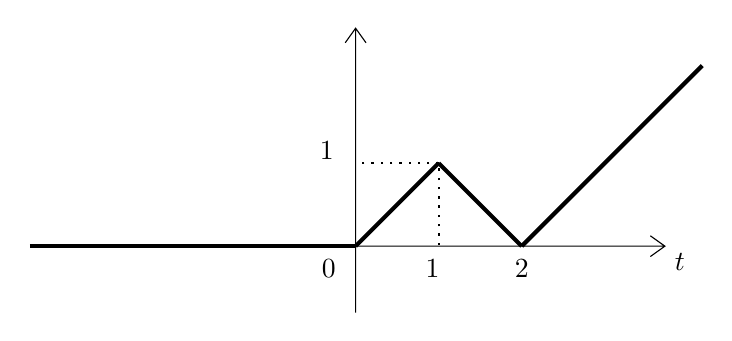
\begin{tikzpicture}[x=0.75pt,y=0.75pt,yscale=-1,xscale=1]
%uncomment if require: \path (0,156); %set diagram left start at 0, and has height of 156

%Shape: Axis 2D [id:dp16516737574733087] 
\draw  (150.5,110) -- (448.5,110)(299.5,5) -- (299.5,142) (441.5,105) -- (448.5,110) -- (441.5,115) (294.5,12) -- (299.5,5) -- (304.5,12)  ;
%Straight Lines [id:da9317289947100813] 
\draw [line width=1.5]    (142.5,110) -- (299.5,110) ;
%Straight Lines [id:da695102507830573] 
\draw [line width=1.5]    (466.48,23.02) -- (379.5,110) ;
%Straight Lines [id:da44710495183723054] 
\draw [line width=1.5]    (339.5,70) -- (299.5,110) ;
%Straight Lines [id:da5381477224930931] 
\draw [line width=1.5]    (379.5,110) -- (339.5,70) ;
%Straight Lines [id:da018036722756767043] 
\draw [line width=0.75]  [dash pattern={on 0.84pt off 2.51pt}]  (339.5,70) -- (299.5,70) ;
%Straight Lines [id:da9481675028243701] 
\draw [line width=0.75]  [dash pattern={on 0.84pt off 2.51pt}]  (339.5,109.39) -- (339.5,70) ;

% Text Node
\draw (281,58.4) node [anchor=north west][inner sep=0.75pt]    {$1$};
% Text Node
\draw (282,115.4) node [anchor=north west][inner sep=0.75pt]    {$0$};
% Text Node
\draw (452,112.4) node [anchor=north west][inner sep=0.75pt]    {$t$};
% Text Node
\draw (332,115.4) node [anchor=north west][inner sep=0.75pt]    {$1$};
% Text Node
\draw (375,115.4) node [anchor=north west][inner sep=0.75pt]    {$2$};


\end{tikzpicture}
\end{figure}
\FloatBarrier

Scriviamo diversamente la $g$
\begin{equation*}
\begin{aligned}
g( t) & =t[ H( t) -H( t-1)] +( 2-t)[ H( t-1) -H( t-2)] +( t-2)[ H( t-2)\\
 & \\
 & \Rightarrow \ \ \mathcal{L}\{g( t)\} =\frac{1}{s^{2}} -2\frac{e^{-s}}{s^{2}} +2\frac{e^{-2s}}{s^{2}}
\end{aligned}
\end{equation*}
\Esercizio{}

Calcolare l'antitrasformata
\begin{equation*}
\mathcal{L}^{-1}\left\{\frac{2s^{2} -4}{( s+1)( s-2)( s-3)}\right\} =\mathcal{L}^{-1}\{( *)\}
\end{equation*}
Scomponiamo in fratti semplici
\begin{equation*}
\begin{aligned}
( *) & =\frac{A}{s+1} +\frac{B}{s-2} +\frac{C}{s-3}\\
 & =\frac{A( s-2)( s-3) +B( s+1)( s-3) +C( s+1)( s-2)}{( s+1)( s-2)( s-3)}\\
 & \Rightarrow \ \ A=-\frac{1}{6} \ \ \ \ B=-\frac{3}{8} \ \ \ \ C=\frac{7}{2}
\end{aligned}
\end{equation*}
Quindi
\begin{equation*}
\begin{aligned}
\mathcal{L}^{-1}\{( *)\} & =\mathcal{L}^{-1}\left\{-\frac{1}{6}\frac{1}{s+1} -\frac{3}{8}\frac{1}{s-2} +\frac{7}{2}\frac{1}{s-3}\right\}\\
 & =\left[ -\frac{1}{6} e^{-t} -\frac{3}{8} e^{2t} +\frac{7}{2} e^{3t}\right] H( t)
\end{aligned}
\end{equation*}
\Esercizio{}

Calcolare l'antitrasformata
\begin{equation*}
\mathcal{L}^{-1}\left\{\frac{3s+1}{( s-1)\left( s^{2} +1\right)}\right\} =\mathcal{L}^{-1}\{( *)\}
\end{equation*}
Scomponiamo in fratti semplici
\begin{equation*}
\begin{aligned}
( *) & =\frac{A}{s-1} +\frac{Bs+C}{\left( s^{2} +1\right)}\\
 & =\frac{A\left( s^{2} +1\right) +( Bs+C)( s-1)}{( s-1)\left( s^{2} +1\right)}\\
 & \Rightarrow \ \ A=2\ \ \ \ C=1\ \ \ \ B=-2
\end{aligned}
\end{equation*}
Quindi
\begin{equation*}
\begin{aligned}
\mathcal{L}^{-1}\{( *)\} & =\mathcal{L}^{-1}\left\{\frac{2}{s-1} +\frac{-2s+1}{s^{2} +1}\right\}\\
 & =\mathcal{L}^{-1}\left\{\frac{2}{s-1} -\frac{2s}{s^{2} +1} +\frac{1}{s^{2} +1}\right\}\\
 & =\left[ 2e^{t} +\sin t-2\cos t\right] H( t)
\end{aligned}
\end{equation*}
\Esercizio{}

Calcolare
\begin{equation*}
\mathcal{L}^{-1}\left\{\frac{1}{( s+3)^{2}}\right\} =e^{-3t} tH( t)
\end{equation*}
Calcolare
\begin{equation*}
\begin{aligned}
\mathcal{L}^{-1}\left\{\frac{e^{-2s}}{s^{3} +s}\right\} & =\mathcal{L}^{-1}\left\{\frac{1}{s}\frac{e^{-2s}}{s^{2} +1}\right\}\\
 & =\int ^{t}_{0}\sin( \tau -2) H( \tau -2) d\tau \\
 & =H( t-2)\int ^{t}_{2}\sin( \tau -2) d\tau \\
 & =H( t-2)[ -\cos( \tau -2)]^{t}_{2}\\
 & =H( t-2)[ 1-\cos( t-2)]
\end{aligned}
\end{equation*}
Calcolare
\begin{equation*}
\begin{aligned}
\mathcal{L}^{-1}\left\{\frac{4e^{-2s}\sinh s}{s^{2} +4}\right\} & =\mathcal{L}^{-1}\left\{\frac{2\left( e^{-s} -e^{-3s}\right)}{s^{2} +4}\right\}\\
 & =\sin[ 2( t-1)] H( t-1) -\sin[ 2( t-3)] H( t-3)
\end{aligned}
\end{equation*}
\Esercizio{}

Determinare le soluzioni $u\in L^{1}(\mathbb{R})$ di
\begin{equation*}
u'-\alpha u=e^{-\alpha x} H( x) \ \ \ \ \alpha  >0
\end{equation*}
\Esercizio{}

Risolvere
\begin{equation*}
u''+2xu'+2u=0
\end{equation*}
\Esercizio{}

Determinare le soluzioni $u\in L^{1}(\mathbb{R})$ di
\begin{equation*}
xu''+2u'-xu=xe^{-| x| }
\end{equation*}
\ParteSoluzioni
\Soluzione

Soluzione nella parte esercizi.
\Soluzione

Soluzione nella parte esercizi.
\Soluzione

Soluzione nella parte esercizi.
\Soluzione

Soluzione nella parte esercizi.
\Soluzione

Soluzione nella parte esercizi.
\Soluzione

Soluzione nella parte esercizi.
\Soluzione

\underline{\textbf{Con l'Analisi 2.}}
\begin{theorem}
Ricordiamo questo risultato di Analisi 2.
\begin{equation*}
y'-\alpha y=f
\end{equation*}
L'integrale generale è
\begin{equation*}
y( x) =Ce^{\alpha x} +y^{\star }( x)
\end{equation*}
\end{theorem}
Nel nostro caso
\begin{equation*}
f( x) =\begin{cases}
0, & x< 0\\
e^{-\alpha x} , & x\geqslant 0
\end{cases}
\end{equation*}
Quindi come equazione particolare
\begin{equation*}
y^{\star }( x) =\begin{cases}
0, & x< 0\\
Ae^{-\alpha x} =-\frac{1}{2\alpha } e^{-\alpha x} , & x\geqslant 0
\end{cases}
\end{equation*}
Quindi l'integrale generale è
\begin{equation*}
\begin{aligned}
y( x) & =\begin{cases}
C_{1} e^{\alpha x} , & x< 0\\
C_{2} e^{\alpha x} -\frac{1}{2\alpha } e^{-\alpha x} , & x\geqslant 0
\end{cases} & C_{1} =C_{2} -\frac{1}{2\alpha }\\
 & =\begin{cases}
Ce^{\alpha x} , & x< 0\\
\left( C+\frac{1}{2\alpha }\right) e^{\alpha x} -\frac{1}{2\alpha } e^{-\alpha x} , & x\geqslant 0
\end{cases} & 
\end{aligned}
\end{equation*}
\underline{\textbf{Con Fourier.}}

Trasformiamo secondo Fourier
\begin{equation*}
\begin{aligned}
\mathcal{F}\left\{e^{-\alpha x} H( x)\right\} & =\int ^{+\infty }_{0} e^{-i\xi x} e^{-\alpha x} dx=\int ^{+\infty }_{0} e^{-( \alpha +i\xi ) x} dx\\
 & =\left[ -\frac{1}{\alpha +i\xi } e^{-( \alpha +i\xi ) x}\right]^{+\infty }_{0} =\frac{1}{\alpha +i\xi }
\end{aligned}
\end{equation*}
Torniamo all'equazione
\begin{equation*}
\begin{aligned}
i\xi \hat{u} -\alpha \hat{u} =\frac{1}{\alpha +i\xi } \ \  & \Rightarrow \ \ ( i\xi -\alpha )\hat{u} =\frac{1}{\alpha +i\xi }\\
 & \Rightarrow \ \ \hat{u} =-\frac{1}{\alpha -i\xi } \cdotp \frac{1}{\alpha +i\xi } =-\frac{1}{\alpha ^{2} +\xi ^{2}}
\end{aligned}
\end{equation*}
Ci ricordiamo che
\begin{equation*}
\mathcal{F}\left\{e^{-\alpha | x| }\right\} =\frac{2\alpha }{\alpha ^{2} +\xi ^{2}} \ \ \Rightarrow \ \ u( x) =-\frac{1}{2\alpha } e^{-\alpha | x| }
\end{equation*}
Ma quelle trovate con l'Analisi 2 dove sono finite?
\begin{equation*}
y( x) \notin L^{1} \ \text{se} \ \left( C+\frac{1}{2\alpha }\right) \neq 0
\end{equation*}
Con Fourier richiediamo che stiano in $L^{1}$ e l'esponenziale positivo causa problemi, quindi per trovare, tra le infinite soluzioni, quella secondo Fourier, dobbiamo porre
\begin{equation*}
C+\frac{1}{2\alpha } =0\ \ \Rightarrow \ \ u( x) =-\frac{1}{2\alpha } e^{-| x| }
\end{equation*}
\Soluzione

È un'equazione lineare del II ordine omogenea, ma \textit{\underline{non a coefficienti costanti}}.
\begin{itemize}
\item $\mathcal{F}\{u\} =\hat{u}$
\item $\mathcal{F}\{u''\} =-\xi ^{2}\hat{u}$
\item $\mathcal{F}\{xu'\} =i\frac{d}{d\xi }\mathcal{F}\{u'\} =i\frac{d}{d\xi }( i\xi \hat{u}) =-(\hat{u} +\xi \hat{u} ')$
\end{itemize}

Allora
\begin{equation*}
\begin{array}{ l }
\Rightarrow \ \ -\xi ^{2}\hat{u} -2\left(\cancel{\hat{u}} +\xi \hat{u} '\right) +\cancel{2\hat{u}} =0\ \ \Rightarrow \ \ 2\xi \hat{u} '+\xi ^{2}\hat{u} =0\\
\Rightarrow \ \ \hat{u} '+\frac{\xi }{2}\hat{u} =0\ \ \Rightarrow \ \ \hat{u}( \xi ) =Ce^{-\frac{\xi ^{2}}{4}}
\end{array}
\end{equation*}
ma
\begin{equation*}
\mathcal{F}\left\{e^{-x^{2}}\right\} =\sqrt{\pi } e^{-\frac{\xi ^{2}}{4}} \ \ \Rightarrow \ \ u( x) =De^{-x^{2}}
\end{equation*}
$u( x)$ dovrebbe essere la combinazione lineare di due integrali particolari, qui abbiamo trovato solo quello che sta in $L^{1}$.
\Soluzione

Trasformiamo
\begin{itemize}
\item $\mathcal{F}\{xu''\} =i\frac{d}{d\xi }\left( -\xi ^{2}\hat{u}\right) =i\left( -2\xi \hat{u} -\xi ^{2}\hat{u} '\right)$
\item $\mathcal{F}\{u'\} =i\xi \hat{u}$
\item $\mathcal{F}\{xu\} =i\hat{u} '$
\item $\mathcal{F}\left\{xe^{-| x| }\right\} =i\frac{d}{d\xi }\frac{2}{1+\xi ^{2}} =i\cdotp \left[\frac{-4\xi }{\left( 1+\xi ^{2}\right)^{2}}\right]$
\end{itemize}

Allora
\begin{equation*}
\begin{aligned}
\cancel{-2i\xi \hat{u}} -i\xi ^{2}\hat{u} '+\cancel{2i\xi \hat{u}} -i\hat{u} ' & =-i\frac{4\xi }{\left( 1+\xi ^{2}\right)^{2}}\\
\left( 1+\xi ^{2}\right)\hat{u} ' & =\frac{4\xi }{\left( 1+\xi ^{2}\right)^{2}}\\
\hat{u} ' & =\frac{4\xi }{\left( 1+\xi ^{2}\right)^{3}} \ \ \Rightarrow \ \ \hat{u}( \xi ) =-\frac{1}{\left( 1+\xi ^{2}\right)^{2}} +c
\end{aligned}
\end{equation*}
dove $c=0$ perché altrimenti non è infinitesima all'infinito e non è la trasformata di alcuna funzione $L^{1}$.

$\hat{u}$ è pari, quindi $u$ è pari.
\chapter{Esercitazione 9 - Potrich}
\ParteEsercizi
\Esercizio{}

Sia
\begin{equation*}
f( x) =H( x) e^{-2x} =\begin{cases}
e^{-2x} , & x\geqslant 0\\
0, & x< 0
\end{cases}
\end{equation*}
calcolare $\displaystyle f*f$ e la sua trasformata di Fourier $\displaystyle \mathcal{F}( f*f)$.
\begin{nb}
[Prodotto di Convoluzione] È definito da
\begin{equation*}
( u*v)( x) =\int _{\mathbb{R}} u( x-y) v( y) dy=\int _{\mathbb{R}} u( y) v( x-y) dy
\end{equation*}
\end{nb}
\Esercizio{}

Determinare la trasformata di Fourier di
\begin{equation*}
f( x) =\ \left( 1-x^{2}\right) H\left( 1-x^{2}\right)
\end{equation*}
Ultilizzando il risultato ottenuto calcolare
\begin{equation*}
I=\int ^{+\infty }_{0}\frac{( x\cos x-\sin x)^{2}}{x^{6}} dx
\end{equation*}
\Esercizio{}
\begin{enumerate}
\item Calcolare la trasformata di Fourier delle funzioni:\begin{equation*}
f_{1}( x) =\frac{1}{1+x^{2}} \ \ \ \ f_{2}( x) =\frac{x}{\left( 1+x^{2}\right)^{2}}
\end{equation*}
\item Considerare la funzione:\begin{equation*}
f_{0}( x) =\arctan\left(\frac{1}{x}\right)
\end{equation*}

Stabilire se $\displaystyle f_{0} \in L^{1}(\mathbb{R})$ e/o se $\displaystyle f_{0} \in L^{2}(\mathbb{R})$.
\item Calcolare la derivata di $\displaystyle f_{0}$ nel senso delle distribuzioni.
\item Calcolare $\mathcal{F}\{f'_{0}\}$ e $\mathcal{F}\{f_{0}\}$.
\end{enumerate}
\Esercizio{}
\begin{definition}
Sia $\displaystyle f:\mathbb{R} \ \rightarrow \mathbb{C}$ si dice Laplace-trasformabile se:
\begin{equation*}
\mathrm{supp} f\subset [ 0,+\infty ) \ \ \ \ \land \ \ \ \ \exists \lambda \in \mathbb{R} :e^{-\lambda t} f( t) \in L^{1}(\mathbb{R})
\end{equation*}
\end{definition}
\begin{definition}
Si dice Ascissa di convergenza di $\displaystyle f$:
\begin{equation*}
\lambda _{f} :=\inf\left\{\lambda \in \mathbb{R} :e^{-\lambda t} f( t) \in L^{1}(\mathbb{R})\right\}
\end{equation*}
\end{definition}
\begin{definition}
Sia $\displaystyle f$ una funzione Laplace-trasformabile, allora la funzione:
\begin{equation*}
\boxed{F( s) :=\int ^{+\infty }_{0} e^{-st} f( t) dt\ \ \ \ \forall s\in \mathbb{C} :\mathrm{Re}( s)  >\lambda _{f}}
\end{equation*}
si dice Trasformata di Laplace di $\displaystyle f$.
\end{definition}
\begin{nb}
[Trasformate di Laplace notevoli] Si ha
\begin{equation*}
\mathcal{L}\{H( t)\} =\frac{1}{s} \ \ \ \ \forall s\in \mathbb{C} :\mathrm{Re}( s)  >\lambda _{f} =0
\end{equation*}
\end{nb}
\begin{theorem}
[Proprietà] Valgono
\begin{itemize}
\item Riscalamento\begin{equation*}
\mathcal{L}\{f( at)\} =\frac{1}{a} F\left(\frac{s}{a}\right) \ \ \ \ \mathrm{Re}( s)  >a\lambda _{f}
\end{equation*}
\item Ritardo\begin{equation*}
\mathcal{L}\{f( t-a)\} =e^{-as} F( s) \ \ \ \ \mathrm{Re}( s)  >\lambda _{f}
\end{equation*}
\item Prodotto con esponenziale\begin{equation*}
\mathcal{L}\left\{e^{at} f( t)\right\} =F( s-a) \ \ \ \ \mathrm{Re}( s)  >\lambda _{f} +\mathrm{Re}( a)
\end{equation*}
\item Linearità\begin{equation*}
\mathcal{L}\{af+bg\} =a\mathcal{L}\{f\} +b\mathcal{L}\{g\} \ \ \ \ \forall a,b\in \mathbb{C} ,\forall s:\mathrm{Re}( s)  >\max\{\lambda _{f} ,\lambda _{g}\}
\end{equation*}
\item Derivata della trasformata\begin{equation*}
\frac{d^{n}}{ds^{n}} F( s) =\mathcal{L}\left\{( -t)^{n} f( t)\right\}
\end{equation*}
\item La primitiva di una funzione $\mathcal{L}$-trasformabile è anch'essa una funzione $\mathcal{L}$-trasformabile\begin{equation*}
\mathcal{L}\left\{\int ^{t}_{0} f( \tau ) d\tau \right\} =\frac{1}{s}\mathcal{L}\{f( t)\} \ \ \ \ \forall s\in \mathbb{C} :\mathrm{Re}( s)  >\max\{\lambda _{f} ,0\}
\end{equation*}
\end{itemize}
\end{theorem}
Detta $\displaystyle H( x)$ la funzione di Heaviside, calcolare la trasformata di Laplace della funzione
\begin{equation*}
f( t) =H( t-1) te^{2t}
\end{equation*}
precisando l'ascissa di convergenza.
\Esercizio{}

Calcolare la trasformata di Laplace di
\begin{equation*}
f( t) =H( t)\sum ^{m}_{k=0} a_{k} t^{k} \ \ \ \ a_{k} \in \mathbb{R}
\end{equation*}
$\displaystyle \lambda _{f} =0$, perché se moltiplichiamo $\displaystyle f$ per $\displaystyle e^{-\lambda t}$ con $\displaystyle \lambda  >0$ le $\displaystyle f$ sono integrabili, 

mentre con $\displaystyle \lambda \leqslant 0$ non lo sono.
\Esercizio{}

Stabilire per quali valori di $\displaystyle a\in \mathbb{R}$ la funzione
\begin{equation*}
f_{a}( x) =H( x) e^{ax^{2} +2x}\sin^{2}( x)
\end{equation*}
è Laplace-trasformabile.

Calcolare poi la trasformata di Laplace di $\displaystyle f_{0}( x)$.
\Esercizio{}

Calcolare la trasformata di Laplace di
\begin{equation*}
f( t) =H( t)\sin( \omega t)
\end{equation*}
studiandone in particolare le trasformate di Laplace per $\displaystyle \omega =1$ e dedurre le antitrasformate di Laplace delle seguenti funzioni:
\begin{equation*}
J( s) =\frac{1}{\left( 1+s^{2}\right)^{2}} \ \ \ \ G( s) =\frac{s}{\left( 1+s^{2}\right)^{2}} \ \ \ \ K( s) =\frac{1}{s\left( s^{2} +4\right)}
\end{equation*}
\ParteSoluzioni
\Soluzione

Se $x< 0$
\begin{equation*}
( f*f)( x) =0
\end{equation*}
Se $x\geqslant 0$ ricordando che l'integrale è non nullo per 
\begin{equation*}
x-y\geqslant 0\ \ \land \ \ x\geqslant 0\ \ \ \ \Leftrightarrow \ \ \ \ y\leqslant x\ \ \land \ \ x\geqslant 0
\end{equation*}
quindi
\begin{align*}
( f*f)( x) & =\int _{\mathbb{R}} f( x-y) f( x) dy=\int ^{x}_{0} e^{-2( x-y)} e^{-2y} dy\\
 & =\int ^{x}_{0} e^{-2x} \ dy=e^{-2x}\int ^{x}_{0} dy=xe^{-2x}
\end{align*}
\begin{theorem}
Date $\displaystyle u,v\in \mathcal{S}(\mathbb{R}) \Rightarrow \ \widehat{u*v} =\hat{u} \cdot \hat{v}$.
\end{theorem}
\begin{align*}
\hat{f}( \xi ) & =\int _{\mathbb{R}} e^{-i\xi x} f( x) dx=\int _{\mathbb{R}} e^{-i\xi x} H( x) e^{-2x} dx=\int ^{+\infty }_{0} e^{-i\xi x} e^{-2x} dx\\
 & =\int ^{+\infty }_{0} e^{-x( i\xi +2)} dx=\left[ -\frac{e^{-x( i\xi +2)}}{i\xi +2}\right]^{+\infty }_{0} =\frac{1}{2+i\xi }\\
 & \\
 & \Rightarrow \ \ \widehat{f*f} =\hat{f} \cdot \hat{f} =\frac{1}{( 2+i\xi )^{2}}
\end{align*}
\Soluzione

Nella scorsa esercitazione:

$f$ pari, allora $\hat{f}$ pari.
\begin{equation*}
\hat{f}( \xi ) =\int _{\mathbb{R}} e^{-i\xi x} f( x) dx=...=4\frac{\sin( \xi ) -\xi \cos( \xi )}{\xi ^{3}}
\end{equation*}
\begin{theorem}
[Identità di Plancherel] Se $\displaystyle u\in L^{2}\left(\mathbb{R}^{n}\right)$
\begin{equation*}
\Vert \hat{u}\Vert _{L^{2}} =( 2\pi )^{n/2}\Vert u\Vert _{L^{2}}
\end{equation*}
oppure elevando tutto alla seconda
\begin{equation*}
\Vert \hat{u}\Vert ^{2}_{L^{2}} =( 2\pi )^{n}\Vert u\Vert ^{2}_{L^{2}} \ \ \Rightarrow \ \ \int _{\mathbb{R}^{n}}| \hat{u}( \xi )| ^{2} d\xi =( 2\pi )^{n}\int _{\mathbb{R}^{n}}| u( x)| ^{2} dx
\end{equation*}
\end{theorem}
Sfrutto il fatto che $f$ e $\hat{f}$ sono pari:
\begin{align*}
\int _{\mathbb{R}}| f( x)| ^{2} dx & =\int ^{1}_{-1}\left( 1-x^{2}\right)^{2} dx=2\int ^{1}_{0}\left( 1-x^{2}\right)^{2} dx\\
 & =2\int ^{1}_{0}\left( 1-2x^2+x^{4}\right) dx=2\left[ x-\frac{2x^{3}}{3} +\frac{x^{5}}{5}\right]^{1}_{0} =\frac{16}{15}\\
 & \\
\int _{\mathbb{R}}| \hat{f}( \xi )| ^{2} d\xi  & =\int ^{+\infty }_{-\infty }\left| 4\frac{(\sin \xi -\xi \ \cos \xi )}{\xi ^{3}}\right| ^{2} d\xi \\
 & =16\int ^{+\infty }_{-\infty }\frac{(\sin \xi -\xi \ \cos \xi )^{2}}{\xi ^{6}} d\xi \\
 & =32\int ^{+\infty }_{0}\frac{(\sin \xi -\xi \ \cos \xi )^{2}}{\xi ^{6}} d\xi =32\cdotp I
\end{align*}
Usando Plancherel
\begin{equation*}
32\cdotp I=( 2\pi )^{n}\int _{\mathbb{R}}| f( x)| ^{2} dx\overset{n=1}{=} 2\pi \cdotp \frac{16}{15} \ \ \Rightarrow \ \ I=\frac{\pi }{15}
\end{equation*}
\Soluzione
\begin{theorem}
[Trasformata della derivata] Date $u,u'\in L^{1}(\mathbb{R})$ e $u\in C^{1}$
\begin{equation*}
\mathcal{F}\left\{\frac{d^{n}}{dx^{n}} u( x)\right\} =( i\xi )^{n} \cdotp \mathcal{F}\{u( x)\}
\end{equation*}
\end{theorem}
\begin{enumerate}
\item Nell'esercitazione scorsa abbiamo visto che:\begin{equation*}
\hat{f}_{1}( \xi ) =\pi e^{-| \xi | } \ \ \ \ \forall \xi \in \mathbb{R}
\end{equation*}Osserviamo che\begin{equation*}
f_{2}( x) =-\frac{1}{2} f_{1} '( x)
\end{equation*}Allora\begin{equation*}
\hat{f}_{2}( \xi ) =-\frac{1}{2}\mathcal{F}( f_{1} '( x) ,\xi ) =-\frac{1}{2} \cdotp i\xi \cdotp \pi e^{-| \xi | } \ \ \ \ \forall \xi \in \mathbb{R}
\end{equation*}
\item Notiamo che $f_{0}$ è limitata, allora $f_{0} \in L^{\infty }(\mathbb{R})$, mentre per $| x| \rightarrow \infty $ è asintotica a $1/x$, che non è integrabile, quindi $f_{0} \notin L^{1}(\mathbb{R})$. Tuttavia $f_{0} \in L^{2}(\mathbb{R})$.
\item $f_{0}$ è continua $\forall x\neq 0$, dove c'è una discontinuità di tipo salto di ampiezza $\pi $. Senza indugi e senza calcoli, deduciamo subito che\begin{equation*}
f_{0} '( x)\overset{D(\mathbb{R})}{=} \pi \delta _{0}( x) -\frac{1}{1+x^{2}}
\end{equation*}
\item Usando le proprietà della trasformata\begin{align*}
\mathcal{F}( f_{0} '( x) ,\xi ) & =\mathcal{F}( \pi \delta _{0} -f_{1}( x) ,\xi ) =\pi -\pi e^{-| \xi | }\\
 & \\
i\xi \cdotp\mathcal{F}( f_{0}( x) ,\xi ) & =\mathcal{F}( f_{0} '( x) ,\xi ) =\pi -\pi e^{-| \xi | }\\
 & \\
 & \Rightarrow \ \ \mathcal{F}( f_{0}( x) ,\xi ) =\frac{\pi -\pi e^{-| \xi | }}{i\xi } =i\pi \frac{e^{-| \xi | } -1}{\xi }
\end{align*}
\end{enumerate}
\Soluzione

Calcoliamo
\begin{equation*}
F( s) =\int ^{+\infty }_{0} e^{-st} f( t) dt=\int ^{+\infty }_{1} e^{-st} te^{2t} dt\ \overset{\text{ipp}}{=}\frac{1-s}{( 2-s)^{2}} e^{2-s}
\end{equation*}
cerco ascissa di convergenza, con $t\geqslant 1$
\begin{equation*}
e^{-\lambda t} te^{2t} =te^{t( 2-\lambda )} \in L^{1}(\mathbb{R}) \ \ \Leftrightarrow \ \ \lambda  >2\ \ \Rightarrow \ \ \lambda _{f} =2
\end{equation*}
\Soluzione

Usiamo le proprietà
\begin{equation*}
F( s) =\mathcal{L}\left\{H( t)\sum ^{m}_{k=0} a_{k} t^{k}\right\} =\sum ^{m}_{k=0} a_{k}\mathcal{L}\left\{H( t) t^{k}\right\} =\sum ^{m}_{k=0} a_{k}( -1)^{k}\left(\frac{1}{s}\right)^{( k)} =( *)
\end{equation*}
Provando vari $\displaystyle k$ mi accorgo che:
\begin{equation*}
( *) =\sum ^{m}_{k=0} a_{k}\frac{k!}{s^{k+1}}
\end{equation*}
È il risultato generale della \textbf{trasformata di un polinomio!}
\Soluzione

Abbiamo che
\begin{equation*}
f_{a}( x) =H( x) e^{ax^{2} +2x}\sin^{2}( x) =\begin{cases}
e^{ax^{2} +2x}\sin^{2}( x) , & x\geqslant 0\\
0, & x< 0
\end{cases}
\end{equation*}
Hanno il supporto in $\displaystyle [ 0,+\infty ) ,\forall a\in \mathbb{R}$. Moltiplichiamo per il solito esponenziale
\begin{equation*}
e^{-\lambda x} f_{a}( x) =\begin{cases}
e^{ax^{2} +( 2-\lambda ) x}\sin^{2}( x) , & x\geqslant 0\\
0, & x< 0
\end{cases} \ \in L^{1} \ \ \Leftrightarrow \ \ a< 0
\end{equation*}
ottengo anche che l'ascissa di convergenza è $\displaystyle \lambda _{f} =-\infty $ poiche $\displaystyle \forall \lambda $ è integrabile.

Nel caso interessato
\begin{equation*}
a=0\ \ \Rightarrow \ \ f_{0}( x) =H( x) e^{2x}\sin^{2}( x)
\end{equation*}
Calcoliamo
\begin{align*}
\mathcal{L}\{f_{0}( x) ,s\} & =\mathcal{L}\left\{H( x) e^{2x}\sin^{2}( x)\right\} \ =\mathcal{L}\left\{H( x) e^{2x}\frac{1-\cos( 2x)}{2}\right\}\\
 & =\frac{1}{2}\mathcal{L}\left\{H( x) e^{2x}\right\} -\frac{1}{2}\mathcal{L}\left\{H( x) e^{2x}\cos( 2x)\right\}\\
 & =\frac{1}{2}\mathcal{L}\left\{H( x) e^{2x}\right\} -\frac{1}{2}\mathcal{L}\left\{H( x) e^{2x}\frac{e^{i2x} +e^{-i2x}}{2}\right\}\\
 & =\frac{1}{2}\mathcal{L}\left\{H( x) e^{2x}\right\} -\frac{1}{4}\mathcal{L}\left\{H( x) e^{2( 1+i) x}\right\} -\frac{1}{4}\mathcal{L}\left\{H( x) e^{2( 1-i) x}\right\}\\
 & =\frac{1}{2} \cdotp \frac{1}{s-2} -\frac{1}{4} \cdotp \frac{1}{s-2( 1+i)} -\frac{1}{4} \cdotp \frac{1}{s-2( 1-i)}\\
 & =\frac{1}{2}\frac{1}{s-2} -\frac{1}{2}\frac{s-2}{( s-2)^{2} +4}
\end{align*}
\Soluzione

Calcoliamo trasformata di $f$
\begin{align*}
\mathcal{L}\{f( t)\} & =\mathcal{L}\{H( t)\sin( \omega t)\} =\mathcal{L}\left\{H( t)\frac{e^{i\omega t} -e^{-i\omega t}}{2i}\right\}\\
 & =\frac{1}{2i}\mathcal{L}\left\{H( t) e^{i\omega t}\right\} -\frac{1}{2i}\mathcal{L}\left\{H( t) e^{-i\omega t}\right\}\\
 & =\frac{1}{2i} \cdotp \frac{1}{s-i\omega } -\frac{1}{2i} \cdotp \frac{1}{s+i\omega }\\
 & =\frac{1}{2i}\frac{s+i\omega -s+i\omega }{s^{2} +\omega ^{2}}\\
 & =\frac{\omega }{s^{2} +\omega ^{2}}
\end{align*}
Funzione $G( s)$.

Notiamo che
\begin{equation*}
\omega =1\ \ \Rightarrow \ \ \mathcal{L}\{H( t)\sin( t)\} =\frac{1}{s^{2} +1} =:\varphi ( s) \ \ \Rightarrow \ \ G( s) =-\frac{1}{2} \varphi '( s)
\end{equation*}
Allora
\begin{equation*}
G( s) =-\frac{1}{2} \varphi '( s) =-\frac{1}{2}\frac{d}{ds}\mathcal{L}\{H( t)\sin( t)\} =\frac{1}{2}\mathcal{L}\{H( t) t\sin( t)\}
\end{equation*}
quindi la sua antitrasformata è
\begin{equation*}
g( t) =\frac{1}{2} H( t) t\sin( t)
\end{equation*}
Funzione $J( s)$.

Notiamo che
\begin{align*}
J( s) & =\frac{1}{s} G( s) =\frac{1}{s}\frac{1}{2}\mathcal{L}\{H( t) t\sin( t)\} =\frac{1}{2}\mathcal{L}\left\{\int ^{t}_{0} H( \tau ) \tau \sin( \tau ) d\tau \right\}\\
 & \overset{\text{ipp}}{=}\frac{1}{2}\mathcal{L}\{(\sin( t) -t\cos( t)) H( t)\}
\end{align*}
quindi la sua antitrasformata è
\begin{equation*}
j( t) =\frac{1}{2}(\sin( t) -t\cos( t)) H( t)
\end{equation*}
Funzione $K( s)$.

Notiamo che
\begin{equation*}
K( s) =\frac{1}{s}\mathcal{L}\left\{\frac{1}{2}H( t)\sin( 2t)\right\} =\frac{1}{2}\mathcal{L}\left\{\int ^{t}_{0} H( \tau )\sin( 2\tau ) d\tau \right\} =\mathcal{L}\left\{\frac{1}{4}( 1-\cos( 2t)) H( t)\right\}
\end{equation*}
quindi la sua antitrasformata è
\begin{equation*}
k( t) =\frac{1}{4}( 1-\cos( 2t)) H( t)
\end{equation*}
\chapter{Esercitazione 10 - Boella}
\ParteEsercizi
\Esercizio{}

Determinare le soluzioni $u\in L^{1}$ di
\begin{equation*}
u+\frac{1}{2} u*e^{-| x| } =e^{-| x| }\cos x
\end{equation*}
\Esercizio{}

Determinare le soluzioni di
\begin{equation*}
\begin{cases}
u''+2u'+u=e^{-t} \chi _{( 1,2)}( t)\\
u( 0) =u'( 0) =0
\end{cases}
\end{equation*}
\Esercizio{}

Determinare le soluzioni $u\in L^{1}$ di
\begin{equation*}
-u''+u=\chi _{( -1,1)}( x)
\end{equation*}
\Esercizio{}

Determinare la soluzione $\mathcal{L}$-trasformabile di
\begin{equation*}
\begin{cases}
u'+2u=2\int ^{t}_{0} u( \tau )\sin( t-\tau ) d\tau +3\cos t\\
u( 0) =1
\end{cases}
\end{equation*}
\Esercizio{}

Determinare le soluzioni $u\in L^{1}$ di
\begin{equation*}
4u+8u''*e^{-| x| } =x^{2} e^{-| x| }
\end{equation*}
\Esercizio{}

Determinare le soluzioni reali $u\in L^{1}$ di
\begin{equation*}
u''+2xu'+4u=0
\end{equation*}
\ParteSoluzioni
\Soluzione
\begin{gather*}
\mathcal{F}\left( e^{-| x| }\right) =\frac{2}{1+\xi ^{2}}\\
\begin{aligned}
\mathcal{F}\left( e^{-| x| }\cos x\right) & =\frac{1}{2}\mathcal{F}\left\{e^{ix} e^{-| x| } +e^{-ix} e^{-| x| }\right\} =\\
 & =\frac{1}{2}\left\{\frac{2}{1+( \xi -1)^{2}} +\frac{2}{1+( \xi +1)^{2}}\right\} =\\
 & =\frac{1}{\xi ^{2} -2\xi +2} +\frac{1}{\xi ^{2} -2\xi +2} =\frac{2\left( \xi ^{2} +2\right)}{\xi ^{4} +4}
\end{aligned}
\end{gather*}
Allora
\begin{equation*}
\hat{u} +\hat{u}\frac{1}{1+\xi ^{2}} =\frac{2\left( \xi ^{2} +2\right)}{\xi ^{4} +4} \ \ \Rightarrow \ \ \hat{u} \cdotp \frac{2+\xi ^{2}}{1+\xi ^{2}} =\frac{2\left( \xi ^{2} +2\right)}{\xi ^{4} +4} \ \ \Rightarrow \ \ \hat{u} =\frac{2\left( 1+\xi ^{2}\right)}{\xi ^{4} +4}
\end{equation*}
Antitrasformiamo
\begin{equation*}
u( x) =\frac{1}{2\pi }\int _{\mathbb{R}} e^{ix\xi }\frac{2\left( 1+\xi ^{2}\right)}{\xi ^{4} +4} d\xi 
\end{equation*}
$\hat{u}$ reale pari, allora $u$ reale pari, quindi studiamo le $x >0$ per poi specchiare.

Usando il Lemma di Jordan (semipiano superiore). Sia
\begin{equation*}
f( z) =\frac{2\left( 1+z^{2}\right) e^{ixz}}{z^{4} +4} \ \ \Rightarrow \ \ u( x) =\frac{1}{2\pi } \cdotp 2\pi i\cdotp \sum _{\mathrm{Im}( z_{k})  >0}\mathrm{Res}( f,z_{k})
\end{equation*}
Il denominatore si annulla in
\begin{equation*}
z^{4} +4=0\ \ \Leftrightarrow \ \ z=\pm 1\pm i
\end{equation*}
Determiniamo i residui
\begin{align*}
\mathrm{Res}( f,1+i) & =\left. \frac{2\left( 1+z^{2}\right) e^{ixz}}{4z^{3}}\right| _{z=1+i} =\left. \frac{2z\left( 1+z^{2}\right) e^{ixz}}{4z^{4}}\right| _{z=1+i}\\
\mathrm{Res}( f,-1+i) & =\left. \frac{2\left( 1+z^{2}\right) e^{ixz}}{4z^{3}}\right| _{z=-1+i} =\left. \frac{2z\left( 1+z^{2}\right) e^{ixz}}{4z^{4}}\right| _{z=-1+i}
\end{align*}
calcoliamo
\begin{align*}
\sum _{\mathrm{Im}( z_{k})  >0}\mathrm{Res}( f,z_{k}) & =-\frac{1}{8}\left\{( 1+i)( 1+2i) e^{( -1+i) x} +( -1+i)( 1-2i) e^{( -1-i) x}\right\}\\
 & =-\frac{e^{-x}}{8}\left\{( -1+3i) e^{ix} +( 1+3i) e^{-ix}\right\}
\end{align*}
Per le $x >0$
\begin{align*}
u( x) & =i\cdotp \sum _{\mathrm{Im}( z_{k})  >0}\mathrm{Res}( f,z_{k})\\
 & =\frac{e^{-x}}{4}\left\{\frac{3+i}{2} e^{ix} +\frac{3-i}{2} e^{-ix}\right\}\\
 & =\frac{e^{-x}}{4}\left\{3\frac{e^{ix} +e^{-ix}}{2} -\frac{e^{ix} -e^{-ix}}{2i}\right\}\\
 & =\frac{e^{-x}}{4}( 3\cos x-\sin x)
\end{align*}
Per le $x\in \mathbb{R}$
\begin{equation*}
u( x) =\frac{e^{-| x| }}{4}( 3\cos x-\sin| x| )
\end{equation*}
\Soluzione
\begin{gather*}
\begin{aligned}
\mathcal{L}\left( e^{-t} \chi _{( 1,2)}( t)\right) & =\int ^{2}_{1} e^{-( s+1) t} dt=\left[ -\frac{e^{-( s+1) t}}{s+1}\right]^{2}_{1}\\
 & =\frac{e^{-s-1}}{s+1} -\frac{e^{-2s-2}}{s+1} =\frac{1}{e}\frac{e^{-s}}{s+1} -\frac{1}{e^{2}}\frac{e^{-2s}}{s+1}
\end{aligned}\\
\\
\mathcal{L}( u) =U( s) \ \ \ \ \mathcal{L}( u') =sU( s) \ \ \ \ \mathcal{L}( u'') =s^{2} U( s)
\end{gather*}
Sostituiamo tutto
\begin{equation*}
\begin{aligned}
U( s)\left[ s^{2} +2s+1\right] & =\frac{1}{e}\frac{e^{-s}}{s+1} -\frac{1}{e^{2}}\frac{e^{-2s}}{s+1}\\
U( s) & =\frac{1}{e}\frac{e^{-s}}{( s+1)^{3}} -\frac{1}{e^{2}}\frac{e^{-2s}}{( s+1)^{3}}
\end{aligned}
\end{equation*}
Antitrasformiamo, ricordiamo che
\begin{equation*}
\mathcal{L}^{-1}\left\{\frac{1}{s^{3}}\right\} =\frac{t^{2}}{2} H( t) \ \ \ \ \mathcal{L}^{-1}\left\{\frac{1}{( s+1)^{3}}\right\} =\frac{t^{2}}{2} e^{-t} H( t) \ \ \ \ \mathcal{L}\{f( t-\alpha )\} =e^{-\alpha s} F( s)
\end{equation*}
allora
\begin{align*}
u( t) & =\frac{1}{e}\frac{( t-1)^{2}}{2} e^{-( t-1)} H( t-1) -\frac{1}{e^{2}}\frac{( t-2)^{2}}{2} e^{-( t-2)} H( t-2)\\
 & =\frac{e^{-t}}{2}\left[( t-1)^{2} H( t-1) -( t-2)^{2} H( t-2)\right]\\
 & =\begin{cases}
0, & t< 1\\
\frac{e^{-t}}{2}( t-1)^{2} , & 1\leqslant t< 2\\
\frac{e^{-t}}{2}( 2t-3) , & t\geqslant 2
\end{cases}
\end{align*}
\Soluzione

Trasformiamo e usiamo il prodotto di convoluzione
\begin{equation*}
\left( \xi ^{2} +1\right)\hat{u} =\mathcal{F}\{\chi _{( -1,1)}( x)\}
\end{equation*}
allora
\begin{align*}
\Rightarrow \ \ \hat{u}( \xi ) & =\frac{1}{1+\xi ^{2}} \cdotp \mathcal{F}\{\chi _{( -1,1)}( x)\}\\
\Rightarrow \ \ u( x) & =\frac{1}{2} e^{-| x| } *\chi _{( -1,1)}( x)
\end{align*}
Ricordiamo che
\begin{equation*}
f*g=\int _{\mathbb{R}} f( t) g( x-t) dt=\int _{\mathbb{R}} f( x-t) g( t) dt
\end{equation*}
Quindi
\begin{equation*}
u( x) =\frac{1}{2}\int _{\mathbb{R}} e^{-| t| } \chi _{( -1,1)}( x-t) dt
\end{equation*}
Dobbiamo dividere i vari casi
\begin{gather*}
\begin{aligned}
\chi _{( -1,1)}( x-t) & =\begin{cases}
1, & -1< x-t< 1\\
0, & \text{altrove}
\end{cases}\\
 & =\begin{cases}
1, & x-1< t< x+1\\
0, & \text{altrove}
\end{cases}
\end{aligned}\\
\\
\Rightarrow \ \ u( x) =\frac{1}{2}\int ^{x+1}_{x-1} e^{-| t| } dt=\begin{cases}
A, & x< -1\\
B, & -1\leqslant x\leqslant 1\\
C, & x >1
\end{cases}
\end{gather*}
analizziamo i vari termini
\begin{align*}
A & =\frac{1}{2}\int ^{x+1}_{x-1} e^{t} dt=\frac{1}{2}\left( e^{x+1} -e^{x-1}\right) =e^{x}\sinh 1\\
B & =\frac{1}{2}\left\{\int ^{0}_{x-1} e^{t} dt+\int ^{x+1}_{0} e^{-t} dt\right\} =\frac{1}{2}\left( 1-e^{x-1} +1-e^{-x-1}\right) =1-e^{-1}\cosh x\\
C & =\frac{1}{2}\int ^{x+1}_{x-1} e^{-t} dt=\frac{1}{2}\left( e^{-x-1} -e^{-x+1}\right) =e^{-x}\sinh 1
\end{align*}
mettendo insieme concludiamo
\begin{equation*}
u( x) =\begin{cases}
1-e^{-1}\cosh x, & | x| < 1\\
e^{-| x| }\sinh 1, & | x| \geqslant 1
\end{cases}
\end{equation*}
\Soluzione
\begin{equation*}
\mathcal{L}( u) =U( s) \ \ \ \ \mathcal{L}( u') =sU( s) -1
\end{equation*}
\begin{align*}
\Rightarrow \ \ sU( s) -1+2U( s) & =2U( s) \cdotp \mathcal{L}\{\sin tH( t)\} +3\mathcal{L}\{\cos t\}\\
sU-1+2U & =U\frac{2}{s^{2} +1} +3\frac{s}{s^{2} +1}\\
U\left( s+2-\frac{2}{s^{2} +1}\right) & =3\frac{s}{s^{2} +1} +1\\
U\cdotp \frac{( s+2)\left( s^{2} +1\right) -2}{\cancel{s^{2} +1}} & =\frac{s^{2} +3s+1}{\cancel{s^{2} +1}}\\
U( s) & =\frac{s^{2} +3s+1}{s^{3} +2s^{2} +s} =\frac{s^{2} +3s+1}{s( s+1)^{2}} =\\
 & =\frac{A}{s} +\frac{Bs+C}{( s+1)^{2}} =\frac{A( s+1)^{2} +( Bs+C) s}{s( s+1)^{2}}\\
 & \\
 & \begin{array}{ l c l }
s=-1 & \rightarrow  & B-C=-1\\
s=1 & \rightarrow  & 4A+B+C=5\\
s=0 & \rightarrow  & A=1\ \ \rightarrow \ \ B=0\ \ C=1
\end{array}\\
 & \ \ \ \ \\
U( s) & =\frac{1}{s} +\frac{1}{( s+1)^{2}}\\
\Rightarrow \ \ u( t) & =H( t) +te^{-t} H( t)\\
 & =\left( 1+te^{-t}\right) H( t)
\end{align*}
\Soluzione

Trasformiamo
\begin{align*}
4\hat{u} -\frac{16\xi ^{2}}{1+\xi ^{2}}\hat{u} & =-\frac{d^{2}}{d\xi ^{2}}\frac{2}{1+\xi ^{2}}\\
\hat{u} \cdotp \frac{4-12\xi ^{2}}{1+\xi ^{2}} & =-\frac{d}{d\xi }\left[\frac{d}{d\xi }\frac{2}{1+\xi ^{2}}\right] =-\frac{d}{d\xi }\left[\frac{-4\xi }{\left( 1+\xi ^{2}\right)^{2}}\right]\\
 & =-\frac{-4\cdotp \left( 1+\xi ^{2}\right)^{2} +4\xi \cdotp 2\left( 1+\xi ^{2}\right) 2\xi }{\left( 1+\xi ^{2}\right)^{4}} =\frac{4-12\xi ^{2}}{\left( 1+\xi ^{2}\right)^{3}}
\end{align*}
quindi
\begin{equation*}
\hat{u} =\frac{1}{\left( 1+\xi ^{2}\right)^{2}}
\end{equation*}
$\hat{u}$ reale pari
\begin{equation*}
u( x) =\frac{1}{2\pi }\int _{\mathbb{R}} e^{ix\xi }\frac{1}{\left( 1+\xi ^{2}\right)^{2}} d\xi 
\end{equation*}
Per $x >0$, usando il lemma di Jordan
\begin{align*}
u( x) & =\frac{1}{\cancel{2\pi }} \cdotp \cancel{2\pi } i\cdotp \mathrm{Res}\left\{\frac{e^{ixz}}{\left( 1+z^{2}\right)^{2}} ,z=i\right\}\\
 & =i\cdotp \frac{d}{dz}\left. \left[\cancel{( z-i)^{2}} \cdotp \frac{e^{ixz}}{( z+i)^{2}\cancel{( z-i)^{2}}}\right]\right| _{z=i}\\
 & =i\cdotp \left. \frac{ixe^{ixz}( z+i)^{2} -e^{ixz} 2( z+i)}{( z+i)^{4}}\right| _{z=i}\\
 & =i\cdotp \frac{1}{16} e^{-x}( -4ix-4i)\\
 & =\frac{1}{4} \ e^{-x}( x+1)
\end{align*}
Per $x\in \mathbb{R}$
\begin{equation*}
u( x) =\frac{e^{-| x| }}{4}(| x| +1)
\end{equation*}
\Soluzione

Trasformiamo i vari termini
\begin{equation*}
\mathcal{F}( u'') =-\xi ^{2}\hat{u} \ \ \ \ \ \ \ \ \mathcal{F}( xu') =i\frac{d}{d\xi }( i\xi \hat{u}) =-\xi \hat{u} '-\hat{u}
\end{equation*}
sostituiamo
\begin{align*}
-\xi ^{2}\hat{u} -2\xi \hat{u} '-2\hat{u} +4\hat{u} & =0\\
-2\xi \hat{u} '+\left( 2-\xi ^{2}\right)\hat{u} & =0\\
\hat{u} '+\frac{2-\xi ^{2}}{-2\xi }\hat{u} & =0
\end{align*}
quindi la trasformata vale
\begin{equation*}
\hat{u}( \xi ) =Ce^{-\int \frac{2-\xi ^{2}}{-2\xi } d\xi } =C\xi e^{-\frac{\xi ^{2}}{4}}
\end{equation*}
$\forall C$, $\hat{u}$ dispari allora $C=D\cdotp i,\ D\in \mathbb{R}$
\begin{equation*}
\ \hat{u}( \xi ) =D\cdotp i\xi e^{-\frac{\xi ^{2}}{4}} \ \ \Rightarrow \ \ u( x) =D\cdotp \frac{d}{dx}\left( e^{-x^{2}}\right) =K\cdotp xe^{-x^{2}}
\end{equation*}
\chapter{Esercitazione 10 - Potrich}
\ParteEsercizi
\Esercizio{}

Determinare le soluzioni $\displaystyle \mathcal{F}$-trasformabili della seguente equazione differenziale
\begin{equation*}
xu''+2u'-xu=xe^{-| x| }
\end{equation*}
\Esercizio{}

Determinare le soluzioni $\displaystyle u\in S'(\mathbb{R})$ dell'equazione differenziale
\begin{equation*}
-u''+u=1+\delta _{0} ''
\end{equation*}
\Esercizio{}

Trovare la soluzione $\mathcal{L}$-trasformabile dell'equazione
\begin{equation*}
\begin{cases}
y'( t) -( t*y)( t) =1\\
y( 0) =-1
\end{cases} \ \ \ \ \text{per} \ t >0
\end{equation*}
\Esercizio{}

Determinare la soluzione $\mathcal{L}$-trasformabile di
\begin{equation*}
\begin{cases}
2y( t) +y'( t) =2\int ^{t}_{0} y( \tau )\sin( t-\tau ) d\tau +3\cos( t)\\
y( 0) =1
\end{cases}
\end{equation*}
\Esercizio{}

Determinare la soluzione del segente problema di Cauchy
\begin{equation*}
\begin{cases}
y''+2y'+y=e^{-t} \chi _{[ 1,2]}( t)\\
y( 0) =y'( 0) =0
\end{cases}
\end{equation*}
\Esercizio{}

Risolvere il problema integro-differenziale
\begin{equation*}
\begin{cases}
y'( t) =1+t+8\int ^{t}_{0}( t-\tau )^{2} y( \tau ) d\tau \\
y( 0) =1
\end{cases}
\end{equation*}
\ParteSoluzioni
\Soluzione

Per le regole di derivazione
\begin{equation*}
\mathcal{F}\left\{u^{( n)}( x)\right\} =( i\xi )^{n}\mathcal{F}\{u( x)\} \ \ \Rightarrow \ \ \mathcal{F}\{u''( x)\} =-\xi ^{2}\mathcal{F}\{u( x)\}
\end{equation*}
e inoltre che
\begin{equation*}
\frac{d^{n}}{d\xi ^{n}}\mathcal{F}\{u( x)\} =\mathcal{F}\left\{( -ix)^{n} u( x)\right\} \ \ \Rightarrow \ \ \mathcal{F}\{xu( x)\} =i\frac{d}{d\xi }\mathcal{F}\{u( x)\}
\end{equation*}
Quindi
\begin{equation*}
\mathcal{F}\{xu''( x)\} =i\frac{d}{d\xi }\left( -\xi ^{2}\mathcal{F}\{u( x)\}\right) =i\left[ -2\xi \hat{u}( \xi ) -\xi ^{2}\frac{d}{d\xi }\hat{u}\right] =-2i\xi \hat{u}( \xi ) -i\xi ^{2}\hat{u} '( \xi )
\end{equation*}
Trasformiamo il secondo termine
\begin{equation*}
\mathcal{F}\left\{e^{-| x| } ,\xi \right\} =\frac{2}{1+\xi ^{2}}
\end{equation*}
Usando le proprietà
\begin{equation*}
\mathcal{F}\left\{xe^{-| x| } ,\xi \right\} =i\frac{d}{d\xi }\frac{2}{1+\xi ^{2}}
\end{equation*}
Otteniamo
\begin{align*}
\cancel{-2i\xi \hat{u}} -i\xi ^{2}\hat{u} '+\cancel{2i\xi \hat{u}} -i\hat{u} ' & =i\frac{d}{d\xi }\frac{2}{1+\xi ^{2}}\\
-\xi ^{2}\hat{u} '-\hat{u} ' & =\frac{d}{d\xi }\frac{2}{1+\xi ^{2}}\\
\hat{u} '\left( 1+\xi ^{2}\right) & =-\frac{d}{d\xi }\frac{2}{1+\xi ^{2}} =-\frac{-2\cdotp 2\xi }{\left( 1+\xi ^{2}\right)^{2}} =\frac{4\xi }{\left( 1+\xi ^{2}\right)^{2}}
\end{align*}
dato che $1+\xi ^{2} \neq 0$
\begin{equation*}
\hat{u} '=\frac{4\xi }{\left( 1+\xi ^{2}\right)^{3}} \ \ \Rightarrow \ \ \hat{u} =-\frac{1}{\left( 1+\xi ^{2}\right)^{2}} +c
\end{equation*}
Affinché $\hat{u}$ sia la trasformata di una funzione trasformabile, questa costante deve essere nulla, altrimenti non sarebbe infinitesima a infinito.
\begin{equation*}
\hat{u} =-\frac{1}{\left( 1+\xi ^{2}\right)^{2}}
\end{equation*}
Andiamo ad antitrasformare.

$\hat{u}$ è reale pari, allora $u$ è reale pari. Per $x >0$
\begin{equation*}
u( x) =\frac{1}{2\pi }\int _{\mathbb{R}} e^{i\xi x}\hat{u}( \xi ) d\xi =\frac{1}{2\pi }\int _{\mathbb{R}} e^{i\xi x}\left[ -\frac{1}{\left( 1+\xi ^{2}\right)^{2}}\right] d\xi =
\end{equation*}
applico il teorema dei residui e il Lemma di Jordan sulla semicirconferenza superiore
\begin{equation*}
=\frac{1}{2\pi }\int _{\mathbb{R}} e^{i\xi x}\left[ -\frac{1}{\left( 1+\xi ^{2}\right)^{2}}\right] d\xi =\frac{1}{2\pi } \cdotp 2\pi i\cdotp \mathrm{Res}\left( -\frac{e^{izx}}{\left( 1+z^{2}\right)^{2}} ,z=i\right) =
\end{equation*}
è un polo del secondo ordine
\begin{equation*}
\begin{aligned}
= & -i\lim\limits _{z\rightarrow i}\frac{d}{dz}\cancel{( z-i)^{2}}\frac{e^{izx}}{\cancel{( z-i)^{2}}( z+i)^{2}} =-i\lim\limits _{z\rightarrow i}\frac{ixe^{izx}( z+i)^{2} -e^{izx} 2( z+i)}{( z+i)^{4}}\\
= & -i\frac{e^{-x}\left[ ix( 2i)^{2} -2( 2i)\right]}{( 2i)^{4}} =-i\frac{e^{-x}[ -2x-2]}{2^{3} i^{3}} =\frac{e^{-x}[ -x-1]}{2^{2}} =-\frac{e^{-x}}{4}( x+1)
\end{aligned}
\end{equation*}
Sfruttiamo la parita. Per $x\in \mathbb{R}$
\begin{equation*}
u( x) =-\frac{e^{-| x| }}{4}(| x| +1)
\end{equation*}
\Soluzione

Risolvo separatamente prima
\begin{equation*}
-u''+u=\delta _{0} ''
\end{equation*}
poi
\begin{equation*}
-u''+u=1
\end{equation*}
infine applico la sovrapposizione degli effetti.

Trasformiamo entrambi i membri
\begin{equation*}
\widehat{u''} =( i\xi )^{2}\hat{u} =-\xi ^{2}\hat{u}
\end{equation*}
Possiamo calcolare la trasformata della derivata della Delta con la dualità
\begin{align*}
\langle \mathcal{F}\{\delta ''( x) ,\xi \} ,\varphi ( x) \rangle  & =\langle \delta ''( x) ,\mathcal{F}\{\varphi ( x) ,\xi \} \rangle \\
 & =-\langle \delta '( x) ,\frac{d}{d\xi }\mathcal{F}\{\varphi ( x) ,\xi \} \rangle \\
 & =\langle \delta ( x) ,\frac{d^{2}}{d\xi ^{2}}\mathcal{F}\{\varphi ( x) ,\xi \} \rangle \\
 & =\langle \delta ( x) ,\mathcal{F}\left\{( -ix)^{2} \varphi ( x) ,\xi \right\} \rangle \\
 & \overset{\xi =0}{=}\int _{\mathbb{R}}( -ix)^{2} \varphi ( x) dx\\
 & =\langle ( -ix)^{2} ,\varphi ( x) \rangle 
\end{align*}
allora
\begin{equation*}
\mathcal{F}\{\delta ''( x) ,\xi \} =( -i\xi )^{2} =-\xi ^{2}
\end{equation*}
Sostituendo nell'equazione
\begin{equation*}
\xi ^{2}\hat{u} +\hat{u} =-\xi ^{2} \ \ \Rightarrow \ \ \left( 1+\xi ^{2}\right)\hat{u} =-\xi ^{2} \ \ \Rightarrow \ \ \hat{u}( \xi ) =-\frac{\xi ^{2}}{1+\xi ^{2}}
\end{equation*}
Notiano che $\hat{u} \notin L^{1}$ quindi per forza dobbiamo ragionare nel senso delle distribuzioni.
\begin{equation*}
\hat{u}( \xi ) =-1+\frac{1}{1+\xi ^{2}} \ \ \Rightarrow \ \ u( x) =-\delta +\frac{1}{2} e^{-| x| }
\end{equation*}
Per quanto riguarda
\begin{equation*}
-u''+u=1
\end{equation*}
l'unica soluzione in $\mathcal{S} '(\mathbb{R})$ è $u( x) =1$, in conclusione
\begin{equation*}
u( x) =1-\delta +\frac{1}{2} e^{-| x| }
\end{equation*}
\Soluzione

Usiamo le proprietà della trasformata di Laplace
\begin{gather*}
\mathcal{L}\{y,s\} =Y( s) \ \ \ \ \mathcal{L}\left\{\frac{d}{dt} y( t) ,s\right\} =sY( s) -y\left( 0^{+}\right)\\
\mathcal{L}\{f*g,s\} =F( s) G( s) \ \ \ \ \mathcal{L}\{tH( t)\} =\frac{1}{s^{2}}
\end{gather*}
Trasformando secondo Laplace i membri dell'equazione
\begin{align*}
sY( s) -\underbrace{y\left( 0^{+}\right)}_{=-1} -\frac{1}{s^{2}} Y( s) & =\frac{1}{s}\\
\left( s-\frac{1}{s^{2}}\right) Y( s) & =\frac{1}{s} -1\\
\frac{s^{3} -1}{s^{\cancel{2}}} Y( s) & =\frac{1-s}{\cancel{s}}\\
\frac{\cancel{( s-1)}\left( s^{2} +s+1\right)}{s} Y( s) & =-\cancel{( s-1)}\\
Y( s) & =-\frac{s}{s^{2} +s+1}
\end{align*}
Dobbiamo antitrasformare, ricordiamo che
\begin{equation*}
\mathcal{L}\{H( t)\cos( \omega t)\} =\frac{s}{s^{2} +\omega ^{2}} \ \ \ \ \mathcal{L}\{H( t)\sin( \omega t)\} =\frac{\omega }{s^{2} +\omega ^{2}}
\end{equation*}
Provo a ricondurmi a queste forme
\begin{equation*}
Y( s) =-\frac{s}{s^{2} +s+1} =-\frac{s+\frac{1}{2} -\frac{1}{2}}{\left( s+\frac{1}{2}\right)^{2} +\frac{3}{4}} =-\frac{s+\frac{1}{2}}{\left( s+\frac{1}{2}\right)^{2} +\frac{3}{4}} +\frac{1}{2}\frac{1}{\left( s+\frac{1}{2}\right)^{2} +\frac{3}{4}}
\end{equation*}
Quindi
\begin{equation*}
y( t) =e^{-\frac{1}{2} t}\left[ -\cos\left(\frac{\sqrt{3}}{2} t\right) +\frac{1}{\sqrt{3}}\sin\left(\frac{\sqrt{3}}{2} t\right)\right]
\end{equation*}
\Soluzione

Trasformiamo i termini di
\begin{equation*}
2y( t) +y'( t) =2\int ^{t}_{0} y( \tau )\sin( t-\tau ) d\tau +3\cos( t)
\end{equation*}
\begin{align*}
\mathcal{L}\{y( t)\} & =Y( s)\\
\mathcal{L}\{y'( t)\} & =sY( s) -y\left( 0^{+}\right)\\
\mathcal{L}\left\{\int ^{t}_{0} y( \tau )\sin( t-\tau ) d\tau \right\} & =\mathcal{L}\{( y*\sin)( t)\} =\mathcal{L}\{y( t)\} \cdotp \mathcal{L}\{\sin( t)\}\\
\mathcal{L}\{H( t)\cos( \omega t)\} & =\frac{s}{s^{2} +\omega ^{2}}\\
\mathcal{L}\{H( t)\sin( \omega t)\} & =\frac{\omega }{s^{2} +\omega ^{2}}
\end{align*}
Sostituiamo
\begin{equation*}
2Y( s) +sY( s) -\underbrace{y\left( 0^{+}\right)}_{=1} =2Y( s) \cdotp \frac{1}{s^{2} +1} +3\frac{s}{s^{2} +1}
\end{equation*}
procediamo coi calcoli per ricavare $Y( s)$
\begin{align*}
\left[ 2+s-\frac{2}{s^{2} +1}\right] Y( s) & =1+\frac{3s}{s^{2} +1}\\
\left[\frac{2\left( s^{2} +1\right) +s\left( s^{2} +1\right) -2}{\cancel{s^{2} +1}}\right] Y( s) & =\frac{s^{2} +1+3s}{\cancel{s^{2} +1}}\\
\left[ 2s^{2} +\cancel{2} +s^{3} +s-\cancel{2}\right] Y( s) & =s^{2} +1+3s\\
s\left( s^{2} +2s+1\right) Y( s) & =s^{2} +1+3s\\
s( s+1)^{2} Y( s) & =s^{2} +1+3s\\
Y( s) & =\frac{s^{2} +1+3s}{s( s+1)^{2}}
\end{align*}
Antitrasformiamo, cerchiamo di ricondurci a qualcosa di noto coi fratti semplici
\begin{nb}
Per scomporre in fratti semplici bisogna seguire alcune regole. Se nella scomposizione del polinomio al denominatore compare:
\begin{equation*}
\begin{array}{ l l }
\text{se a denom. c'è:} & \text{allora si associa}\\
x-a & \frac{A}{x-a}\\
(x-a)^{n} & \frac{A_{1}}{x-a} +\frac{A_{2}}{(x-a)^{2}} +\dotsc +\frac{A_{n}}{(x-a)^{n}}\\
 \begin{array}{l}
x^{2} +bx+c\\
( \Delta < 0)
\end{array} & \frac{Ax+B}{x^{2} +bx+c}\\
 \begin{array}{l}
\left( x^{2} +bx+c\right)^{n}\\
( \Delta < 0)
\end{array} & \frac{A_{1} x+B_{1}}{x^{2} +bx+c} +\frac{A_{2} x+B_{2}}{\left( x^{2} +bx+c\right)^{2}} +\dotsc +\frac{A_{n} x+B_{n}}{\left( x^{2} +bx+c\right)^{n}}
\end{array}
\end{equation*}
\end{nb}
\begin{equation*}
\frac{s^{2} +1+3s}{s( s+1)^{2}} =\frac{A}{s} +\frac{Bs+C}{( s+1)^{2}} =\frac{A( s+1)^{2} +s( Bs+C)}{s( s+1)^{2}} =\dotsc 
\end{equation*}
Otteniamo
\begin{equation*}
Y( s) =\frac{s^{2} +1+3s}{s( s+1)^{2}} =\frac{1}{s} +\frac{1}{( 1+s)^{2}}
\end{equation*}
Ricordando
\begin{equation*}
\mathcal{L}\{tH( t)\} =\frac{1}{s^{2}} \ \ \ \ \mathcal{L}\left\{e^{\alpha t} f( t)\right\} =F( s-\alpha )
\end{equation*}
Si ottiene
\begin{equation*}
y( t) =H( t) +tH( t) e^{-t} =H( t)\left( 1+te^{-t}\right)
\end{equation*}
\Soluzione

Per risolvere
\begin{equation*}
y''+2y'+y=e^{-t} \chi _{[ 1,2]}( t)
\end{equation*}
trasformiamo e usiamo le proprietà
\begin{align*}
\mathcal{L}\{y( t)\} & =Y( s)\\
\mathcal{L}\{y'( t)\} & =sY( s) -\cancel{y\left( 0^{+}\right)} =sY( s)\\
\mathcal{L}\{y''( t)\} & =s\left( sY( s) -\cancel{y\left( 0^{+}\right)}\right) -\cancel{y'\left( 0^{+}\right) \ } =s^{2} Y( s)\\
\mathcal{L}\left\{e^{-t} \chi _{[ 1,2]}( t)\right\} & =\int ^{\infty }_{0} e^{-st} e^{-t} \chi _{[ 1,2]}( t) dt=\int ^{2}_{1} e^{-( s+1) t} dt\\
 & =\left[ -\frac{e^{-( s+1) t}}{s+1}\right]^{2}_{1} =\frac{e^{-( s+1)} -e^{-2( s+1)}}{s+1} =\frac{e^{-s}}{e( s+1)} -\frac{e^{-2s}}{e^{2}( s+1)}
\end{align*}
Sostituiamo nell'equazione
\begin{align*}
s^{2} Y( s) +2sY( s) +Y( s) & =\frac{e^{-s}}{e( s+1)} -\frac{e^{-2s}}{e^{2}( s+1)}\\
( s+1)^{2} Y( s) & =\frac{e^{-s}}{e( s+1)} -\frac{e^{-2s}}{e^{2}( s+1)}\\
Y( s) & =\frac{e^{-s}}{e( s+1)^{3}} -\frac{e^{-2s}}{e^{2}( s+1)^{3}}
\end{align*}
Per antitrasformare notiamo che
\begin{gather*}
\mathcal{L}\left\{e^{\alpha t} f( t)\right\} =F( s-\alpha ) \ \ \ \ \mathcal{L}\left\{t^{2} H( t)\right\} =( -1)^{2}\frac{d^{2}}{ds^{2}}\frac{1}{s} =\frac{d}{ds}\left( -\frac{1}{s^{2}}\right) =\frac{2}{s^{3}}\\
\mathcal{L}\{f( t-\alpha )\} =e^{-\alpha s} F( s)
\end{gather*}
Allora
\begin{gather*}
\mathcal{L}\left\{\frac{1}{2} t^{2} H( t)\right\} =\frac{1}{s^{3}} \ \ \Rightarrow \ \ \mathcal{L}\left\{\frac{1}{2} t^{2} H( t) e^{-t}\right\} =\frac{1}{( s+1)^{3}}\\
\Rightarrow \ \ \mathcal{L}\left\{\frac{1}{2}( t-1)^{2} H( t-1) e^{-( t-1)}\right\} =\frac{e^{-s}}{( s+1)^{3}}
\end{gather*}
Quindi
\begin{equation*}
y( t) =\frac{1}{e} \cdotp \frac{1}{2}( t-1)^{2} H( t-1) e^{-( t-1)} -\frac{1}{e^{2}}\frac{1}{2}( t-2)^{2} H( t-2) e^{-( t-2)}
\end{equation*}
\Soluzione

Per risolvere
\begin{equation*}
y'( t) =1+t+8\int ^{t}_{0}( t-\tau )^{2} y( \tau ) d\tau 
\end{equation*}
antitrasformiamo
\begin{align*}
\mathcal{L}\{y'( t)\} & =sY( s) -y\left( 0^{+}\right) =sY( s) -1\\
\mathcal{L}\{1H( t)\} & =\frac{1}{s}\\
\mathcal{L}\{tH( t)\} & =( -1)^{1}\frac{d}{ds}\frac{1}{s} =\frac{1}{s^{2}}\\
\mathcal{L}\left\{\int ^{t}_{0}( t-\tau )^{2} y( \tau ) d\tau \right\} & =\mathcal{L}\left\{t^{2} *y( t)\right\} =\mathcal{L}\left\{t^{2} H( t)\right\} \cdotp \mathcal{L}\{y( t)\}\\
 & =\frac{2}{s^{3}} \cdotp Y( s)
\end{align*}
Sostituiamo nell'equazione
\begin{align*}
sY( s) -1 & =\frac{1}{s} +\frac{1}{s^{2}} +8\cdotp \frac{2}{s^{3}} \cdotp Y( s)\\
\left( s-\frac{16}{s^{3}}\right) Y( s) & =\frac{1}{s} +\frac{1}{s^{2}} +1\\
\left(\frac{s^{4} -16}{s^{3}}\right) Y( s) & =\frac{s+1+s^{2}}{s^{2}}\\
\left(\frac{\left( s^{2} +4\right)\left( s^{2} -4\right)}{s}\right) Y( s) & =s+1+s^{2}\\
Y( s) & =\frac{s\left( s+1+s^{2}\right)}{\left( s^{2} +4\right)( s+2)( s-2)}
\end{align*}
Scomponiamo in fratti semplici
\begin{align*}
\frac{s\left( s+1+s^{2}\right)}{\left( s^{2} +4\right)( s+2)( s-2)} & =\frac{As+B}{s^{2} +4} +\frac{C}{s+2} +\frac{D}{s-2}\\
\frac{s^{2} +s+s^{3}}{\left( s^{2} +4\right)( s+2)( s-2)} & =\frac{( As+B)\left( s^{2} -4\right) +C\left( s^{2} +4\right)( s-2) +D\left( s^{2} +4\right)( s+2)}{\left( s^{2} +4\right)( s+2)( s-2)}\\
 & =\frac{As^{3} +Bs^{2} -4As-4B+C\left( s^{3} -2s^{2} +4s-8\right)}{\left( s^{2} +4\right)( s+2)( s-2)}\\
 & \ \ \ \ +\frac{D\left( s^{3} +2s^{2} +4s+8\right)}{\left( s^{2} +4\right)( s+2)( s-2)}\\
 & =\frac{s^{3}( A+C+D) +s^{2}( B-2C+2D) +s( -4A+4C+4D)}{\left( s^{2} +4\right)( s+2)( s-2)}\\
 & +\frac{-4B-8C+8D}{\left( s^{2} +4\right)( s+2)( s-2)}
\end{align*}
Uguagliamo i polinomi
\begin{equation*}
\begin{aligned}
1 & =A+C+D\\
1 & =B-2C+2D\\
1 & =-4A+4C+4D\\
0 & =-4B-8C+8D
\end{aligned} \ \ \Leftrightarrow \ \ \begin{bmatrix}
1 & 0 & 1 & 1\\
0 & 1 & -2 & 2\\
-4 & 0 & 4 & 4\\
0 & -4 & -8 & 8
\end{bmatrix}\begin{bmatrix}
A\\
B\\
C\\
D
\end{bmatrix} =\begin{bmatrix}
1\\
1\\
1\\
0
\end{bmatrix}
\end{equation*}
che ha come soluzione\footnote{Ovviamente trovata a mente e senza usare Matlab.}
\begin{equation*}
\begin{bmatrix}
A\\
B\\
C\\
D
\end{bmatrix} =\begin{bmatrix}
3/8\\
1/2\\
3/16\\
7/16
\end{bmatrix}
\end{equation*}
Quindi
\begin{equation*}
Y( s) =\frac{\frac{3}{8} s+\frac{1}{2}}{s^{2} +4} +\frac{3}{16( s+2)} +\frac{7}{16( s-2)}
\end{equation*}
Notiamo che
\begin{equation*}
\frac{\frac{3}{8} s+\frac{1}{2}}{s^{2} +4} =\frac{3}{8} \cdotp \frac{s}{s^{2} +4} +\frac{1}{2} \cdotp \frac{1}{s^{2} +4}
\end{equation*}
Antitrasformiamo
\begin{align*}
\mathcal{L}^{-1}\left\{\frac{3}{8} \cdotp \frac{s}{s^{2} +4}\right\} & =\frac{3}{8}\mathcal{L}^{-1}\left\{\frac{s}{s^{2} +4}\right\} =\frac{3}{8}\cos( 2t) H( t)\\
\mathcal{L}^{-1}\left\{\frac{1}{2} \cdotp \frac{1}{s^{2} +4}\right\} & =\frac{1}{4}\mathcal{L}^{-1}\left\{\frac{2}{s^{2} +4}\right\} =\frac{1}{4}\sin( 2t) H( t)
\end{align*}
In conclusione
\begin{equation*}
y( s) =\left[\frac{7}{16} e^{2t} +\frac{3}{16} e^{-2t} +\frac{3}{8}\cos( 2t) +\frac{1}{4}\sin( 2t)\right] H( t)
\end{equation*}



\end{document}